\section{Methods}
\label{sec:perception_methods}


This section divides into three parts, which are shown in \figref{fig:perception_methods_flowchart}.
The a) hardware setup, namely the robots and camera, is presented in~\secref{ssec:perception_methods_hardwaresetup}.
The next section, \secref{ssec:perception_methods_noiseandoutlierdetection} shows b) how to detect noise and outliers and how to remove them.
The filter is described in the discrete, as well as continuous domain.
In c),~\secref{ssec:perception_methods_visualodometryalgorithm}, the algorithms to compute a pose update based only on Visual Odometry on embedded hardware are shown. 

\begin{figure}[]
  \centering
  % Define block styles
\tikzstyle{block} = [draw, rectangle, fill=white, minimum height=3.5cm, minimum width=6.0cm, text width=4.5cm, text centered, rounded corners=true]
\tikzstyle{blockBox} = [draw, inner sep=0.2cm, dashed, rectangle, minimum width=3.5cm, text centered, rounded corners=true]
\tikzstyle{blockText} = [text centered, minimum height=1.5cm,text width=5.0cm]
\tikzstyle{arrow} = [draw, -latex]

\definecolor{red1}{RGB}{160,0,0}
\definecolor{green1}{RGB}{0,160,0}
\definecolor{blue1}{RGB}{0,0,160}

% Define images
\pgfdeclareimage[height=3.0cm]{scene}{./figures/sensor/methods_flowchart_scene.jpg}
\pgfdeclareimage[height=3.0cm]{robot}{./figures/sensor/methods_flowchart_robot.jpg}
	      
\begin{tikzpicture}[node distance = 8.0cm, auto]
  % Scene
  \node[block] (scene) {\pgfuseimage{scene}};

  % Hardware setup
  \node [block, right of=scene] (hardwaresetup) {\pgfuseimage{robot}};

	% Filter
  \node [block, below of=scene, node distance=6.5cm] (filter) {Removing noise and outliers};
  
  % VO
  \node [block, right of=filter] (vo) {Estimating pose, position, and environment};
  

  % Text
  \node [blockText, above of=scene, node distance=2.5cm] (scene_t) {\textbf{a) Scene}};
  \node [blockText, above of=hardwaresetup, node distance=2.5cm] (hardwaresetup_t) {\textbf{b) Hardware setup}\\\secref{ssec:perception_methods_hardwaresetup}};
  \node [blockText, above of=filter, node distance=2.5cm] (filter_t) {\textbf{c) Preprocessing}\\\secref{ssec:perception_methods_noiseandoutlierdetection}};
  \node [blockText, above of=vo, node distance=2.5cm] (vo_t) {\textbf{d) Visual Odometry}\\\secref{ssec:perception_methods_visualodometryalgorithm}};


  % Fit
  \node[fit=(scene)(scene_t), blockBox] (scene_f) {};
  \node[fit=(hardwaresetup)(hardwaresetup_t), blockBox] (hardwaresetup_f) {};
  \node[fit=(filter)(filter_t), blockBox] (filter_f) {};
  \node[fit=(vo)(vo_t), blockBox] (vo_f) {};


  % Arrows
	\path [arrow] (scene_f.east) to (hardwaresetup_f.west);
	\path [arrow] (hardwaresetup_f.south) -| ++(0,-0.55cm) -| (filter_f.north);
	\path [arrow] (filter_f.east) to (vo_f.west);
\end{tikzpicture}

  \caption{Flowchart of the methods in this chapter and how they relate. Details are explained in \secref{sec:perception_methods}.}
  \label{fig:perception_methods_flowchart}
\end{figure}





\subsection{Hardware setup}
\label{ssec:perception_methods_hardwaresetup}

The hardware setup is depicted in \figref{fig:robot_introduction_photo}: A quadrocopter and a wheeled robot, both controlled by a Raspberry Pi mini computer.
As the focus lies on denoising and \gls{ac:vo} in this part of the thesis, mostly the quadrotor platform will be analyzed --- it is fast moving and therefore more demanding.
In order to cope with high turn rates in indoor environments, a catadioptric omnidirectional system is used.
It is composed of an upwards pointing monocular camera and a hyperbolic mirror above as shown in \figref{fig:robot_method_algorithms_mirror_hyperbolaphoto}.
The camera operates with a resolution of $\unit[480 \times\ 480]{px}$ at a frequency of \unit[30]{Hz}.
Additionally to the computer vision system, an \gls{ac:imu} is placed on the robot.
All software components run as modular and parallel nodes using \gls{ac:ros}.





\subsection{Noise and outlier detection}
\label{ssec:perception_methods_noiseandoutlierdetection}

Let $\Phi(i, j)$ be the observed image. 
Then the noisy image is defined as
\begin{align}
  \Phi\left(i,j\right) = u\left(i,j\right) + n\left(i,j\right),
\end{align}
where $u\left(i,j\right)$ is the ``true'' value and $n\left(i,j\right)$ is noise at image position $\left(i,j\right)^T$. 
Here, noise is modeled as Gaussian white noise, meaning $n\left(i,j\right)$ is Gaussian distributed with zero mean and variance $\sigma^2$.
Additionally, salt-and-pepper noise is added: a fixed percentage of color channels will be set to either $0$ or its maximum value.
The filter $D_h$, with filter parameter $h$, is defined as follows
\begin{align}
  \Phi &= D_{h}(\Phi) + n
\end{align}
meaning, that for an optimal filter
\begin{align}
  u &= D_h(u+n)
\end{align}
should be true. 
The filter parameter $h$ should depend only on the variance of the noise $h = h(\sigma)$. 
Later, for evaluation the \gls{ac:rmse} and \gls{ac:psnr} between the original image $u$ and the filtered $D_h(u+n)$ is computed.


\begin{figure}[t]
  \centering
  % Define block styles
\tikzstyle{block} = [draw, rectangle, fill=white, minimum height=3cm, minimum width=3.9cm, text width=3.7cm, text centered, rounded corners=true]
\tikzstyle{blockBox} = [draw, inner sep=0.2cm, dashed, rectangle, minimum width=3.5cm, text centered, rounded corners=true]
\tikzstyle{blockText} = [text centered, minimum height=1.5cm,text width=3.9cm]
\tikzstyle{arrow} = [draw, -latex]

\definecolor{red1}{RGB}{160,0,0}
\definecolor{green1}{RGB}{0,160,0}
\definecolor{blue1}{RGB}{0,0,160}

% Define images
\pgfdeclareimage[height=2.4cm]{noisy}{./figures/perception/methods/noiseandoutlierremoval/flowchart_noisy_frame.jpg}
\pgfdeclareimage[height=2.2cm]{smooth}{./figures/perception/methods/noiseandoutlierremoval/flowchart_smooth.jpg}
\pgfdeclareimage[height=1.0cm]{threshold}{./figures/perception/methods/noiseandoutlierremoval/flowchart_threshold.png}
\pgfdeclareimage[height=2.4cm]{filtered}{./figures/perception/methods/noiseandoutlierremoval/flowchart_edgefilter.jpg}


\begin{tikzpicture}[node distance = 5.0cm, auto]
  % Noisy image
  \node[block] (noisy) {\pgfuseimage{noisy}};

  % Smoothing
  \node [block, right of=noisy] (smooth) {\pgfuseimage{smooth}};

  % Distance Matrix
  \node [block, right of=smooth] (matrix) {$%
     \begin{bmatrix}
       \delta_{0,0} & \delta_{0,1} & \ldots       & \delta_{0,k} \\
       \delta_{1,0} & \delta_{1,1} &              & \ldots \\
       \ldots       &              & \ldots       & \\
       \delta_{l,0} & \ldots       &              & \delta_{l,k}
     \end{bmatrix}$%
   };
  

  % Threshold
  \node [block, below of=noisy, node distance=6.0cm] (threshold) {\pgfuseimage{threshold}};
  
  % Filtered result
  \node [block, right of=threshold] (filtered) {\pgfuseimage{filtered}};
  
  
  % Text
  \node [blockText, above of=noisy, node distance=2.2cm] (noisy_t) {\textbf{a) Division into subwindows $\Psi$}};
  \node [blockText, above of=smooth, node distance=2.2cm] (smooth_t) {\textbf{b) Smoothing}};
  \node [blockText, above of=matrix, node distance=2.2cm] (matrix_t) {\textbf{c) Distance matrices $\Delta$ and $\delta_m$}};
  \node [blockText, above of=threshold, node distance=2.2cm] (threshold_t) {\textbf{d) Apply threshold $\tau$}};
  \node [blockText, above of=filtered, node distance=2.2cm] (filtered_t) {\textbf{e) Compute weight}};


  % Fit
  \node[fit=(noisy)(noisy_t), blockBox] (noisy_f) {};
  \node[fit=(smooth)(smooth_t), blockBox] (smooth_f) {};
  \node[fit=(matrix)(matrix_t), blockBox] (tranform_f) {};
  \node[fit=(threshold)(threshold_t), blockBox] (threshold_f) {};
  \node[fit=(filtered)(filtered_t), blockBox] (filtered_f) {};


  % Arrows
  \path [arrow] (noisy_f.east) to (smooth_f.west);
  \path [arrow] (smooth_f.east) to (tranform_f.west);
  \path [arrow] (tranform_f.south) -| ++(0,-0.55cm) -| (threshold_f.north);
  \path [arrow] (threshold_f.east) to (filtered_f.west);
\end{tikzpicture}

    \caption{Overview of the system structure. A detailed explanation of all steps is shown in \secref{ssec:perception_methods_noiseandoutlierdetection}.}
  \label{fig:perception_methods_noiseandoutlierremoval_flowchart}
\end{figure}

A flowchart of the proposed algorithm \gls{ac:epf} is shown in \figref{fig:perception_methods_noiseandoutlierremoval_flowchart}, a detailed explanation of all steps follows in the next sections.
First, the image $\Phi$ is divided into a) subwindows $\Psi$ sized $N = k \cdot l$, where each subwindow is shifted by one pixel relative to the last one, such that there are as many subwindows as there are pixels in the image. 
Each subwindow is then b) smoothed using a Gaussian kernel. 
Subwindow size $k \times l$ and Gaussian smoothing parameter are hyperparameters, which need to be manually tuned.
However, all three heavily depend on the amount of noise you would want to remove. 
For each subwindow centered around pixel position $(i, j)^T$ a c) distance matrix $\Delta_{i,j}$ and a mean distance $\delta_{i,j}^m$ is computed in the color domain. 
This offers a measurement for noise, as described below. 
A user selected d) threshold $\tau$, which defines a threshold between noise and a mere color edge, is applied to $\Delta_{i,j}$ and $\delta_{i,j}^m$. 
In case of noise, e) a weight $\omega_{i,j}$ is computed, which will move the color values of the pixel in the subwindow to the mean color of the subwindow.

\begin{figure}
    \centering
    \includegraphics[width=0.75\textwidth]{./figures/sensor/method_boundaryconditions.jpg}
    \caption{Periodic mirrored boundary conditions are used for image subwindows. A red rectangle denotes borders of original image.}
    \label{fig:method_boundaryconditions}
\end{figure}





\subsubsection{Division into subwindows} 

Let one pixel at position $(i, j)^T$ contain the color information
\begin{eqnarray}
   \bm{\varphi}_{i,j} = ( \varphi_{i,j}^r,\ \varphi_{i,j}^g,\ \varphi_{i,j}^b )^T. 
\end{eqnarray}
A subwindow $\Psi^{\left(i,j\right)}$ is created around $(i, j)^T$, such that $(i, j)^T$ is centered. 
In case the subwindow contains an image boundary, periodic mirrored boundary conditions are used as visualized in \figref{fig:method_boundaryconditions}. 
The size of the subwindow is defined by $k \times l$ and a pixel's position inside the subwindow will be denoted by $(r, s)^T$.
This implies $0 \leq r < k$ and $0 \leq s < l$. 
Please note that other than rectangular shaped windows are possible.
In this work, additionally disc-shaped and Gaussian shaped subwindows were tried, however results differed only marginally.





\subsubsection{Smoothing} 

Each subwindow is smoothed via a Gaussian kernel~\cite[p. 257f]{gonzalezwoods2002}. 
This removes outliers, which would otherwise distort the computation of the mean as described in the next step.





\subsubsection{Computation of the distance matrix}

For each subwindow $\Psi^{\left(i,j\right)}$ the arithmetic mean is calculated as
\begin{eqnarray}
  \bm{\psi}_{m}^{\left(i,j\right)} = \frac{1}{N} \left( \sum_{r,s} \psi_{r,s}^r,\ \sum_{r,s} \psi_{r,s}^g,\ \sum_{r,s} \psi_{r,s}^b \right)^T
\end{eqnarray}
where $N = k \cdot l$ denotes the size of the subwindow. The pixelwise distances
\begin{eqnarray}
  \delta_{r,s}^{\left(i,j\right)} = | \bm{\psi}_{r,s} - \bm{\psi}_{m}^{\left(i,j\right)} |_2
\end{eqnarray}
are stored in a matrix $\Delta^{\left(i,j\right)}$. Furthermore, for each subwindow $\Psi^{\left(i,j\right)}$ the mean pixelwise distance 
\begin{eqnarray}
  \delta_m^{\left(i,j\right)} = \frac{1}{N} \sum_{r,s} \delta_{r,s}^{\left(i,j\right)}
\end{eqnarray}
is calculated.





\subsubsection{Thresholding}

Using a threshold it is now analyzed, whether a subwindow contains a color edge (and therefore no pixels should be smoothed), whether one pixel contains an outlier (and should be corrected), or neither, which means the pixel value should also not be replaced.
If $\delta_m^{\left(i,j\right)}$ is large, the subwindow contains big color variations.
This means the subwindow includes a color edge.
If $\delta_m^{\left(i,j\right)}$ is small, but one single pixel holds a big color variations (large $\delta_{r,s}^{\left(i,j\right)}$), there is an outlier, which needs to be replaced.
If both, $\delta_m^{\left(i,j\right)}$ and $\delta_{r,s}^{\left(i,j\right)}$ are small, the pixel holds a ``normal color'' value.
A threshold $\tau$ is introduced to identify noisy pixels and color edges, yielding
\begin{eqnarray}
  \psi_{r,s} =  \begin{cases}
    \textrm{color\ edge} & \textrm{,\ if\ } \delta_m^{\left(i,j\right)} > \tau, \\
    \textrm{noise} & \textrm{,\ if\ } \delta_m^{\left(i,j\right)} \leq \tau \textrm{\ and\ } \delta_{r,s} > \tau, \\
    \textrm{neither} & \textrm{,\ else}.
  \end{cases} \label{eqn:decision_noise_edge}
\end{eqnarray}





\subsubsection{Update of RGB values}

A new image $\Theta$, holding the pixel values $\bm{\theta}_{i,j}$ is computed based upon the squared distance of the user based threshold $\tau$ and the pixelwise distance $\delta_{r,s}$. 
$\bm{\theta}_{i,j}$ is updated as follows
\begin{eqnarray}
  \bm{\theta}_{i,j} &\longleftarrow& \bm{\theta}_{i,j} + \psi_{r,s} \cdot \left( \tau - \delta_{r,s}^{\left(i,j\right)} \right)^2 \cdot \bm{\psi}_{m}^{\left(i,j\right)}.
\end{eqnarray}
Please note, that due to the sliding subwindows each pixel is updated $N= k \cdot l$ times and therefore needs to be normalized. Thus, an additional weight $\Omega$ is introduced for each pixel $\omega_{i,j}$ as
\begin{eqnarray}
  \omega_{i,j} &\longleftarrow& \omega_{i,j} + \psi_{r,s} \cdot \left( \tau - \delta_{r,s}^{\left(i,j\right)} \right)^2.
  \label{eq:method_weightupdate}
\end{eqnarray}
The final image results from division of $\Theta$ by $\Omega$. 
In rare cases $\tau = \delta_{r,s}^{\left(i,j\right)}$ for large image patches may happen, which will result in $\omega_{i,j} = 0$ according to \eqnref{eq:method_weightupdate}.
To avoid division by zero it is suggested to initialize $\Omega$ with ones instead of zeros (since in general $\omega_{i,j} \gg 0$, this does not change the final outcome significantly).

\begin{figure}
  \centering
  \begin{tikzpicture}[gnuplot]
%% generated with GNUPLOT 5.2p2 (Gentoo revision r0) (Lua 5.1; terminal rev. 99, script rev. 102)
%% Fri 08 Jun 2018 01:36:24 PM CEST
\gpcolor{color=gp lt color border}
\gpsetlinetype{gp lt border}
\gpsetdashtype{gp dt solid}
\gpsetlinewidth{1.00}
\draw[gp path] (1.354,1.842)--(1.568,1.842);
\node[gp node right] at (1.354,1.842) {$10$};
\draw[gp path] (1.354,3.176)--(1.568,3.176);
\node[gp node right] at (1.354,3.176) {$20$};
\draw[gp path] (1.354,4.508)--(1.568,4.508);
\node[gp node right] at (1.354,4.508) {$30$};
\draw[gp path] (1.354,5.842)--(1.568,5.842);
\node[gp node right] at (1.354,5.842) {$40$};
\draw[gp path] (1.354,7.176)--(1.568,7.176);
\node[gp node right] at (1.354,7.176) {$50$};
\draw[gp path] (1.354,8.508)--(1.568,8.508);
\node[gp node right] at (1.354,8.508) {$60$};
\draw[gp path] (1.354,1.175)--(1.354,1.390);
\node[gp node center] at (1.354,0.808) {$0$};
\draw[gp path] (2.414,1.175)--(2.414,1.390);
\node[gp node center] at (2.414,0.808) {$10$};
\draw[gp path] (3.475,1.175)--(3.475,1.390);
\node[gp node center] at (3.475,0.808) {$20$};
\draw[gp path] (4.536,1.175)--(4.536,1.390);
\node[gp node center] at (4.536,0.808) {$30$};
\draw[gp path] (5.596,1.175)--(5.596,1.390);
\node[gp node center] at (5.596,0.808) {$40$};
\draw[gp path] (6.657,1.175)--(6.657,1.390);
\node[gp node center] at (6.657,0.808) {$50$};
\draw[gp path] (7.717,1.175)--(7.717,1.390);
\node[gp node center] at (7.717,0.808) {$60$};
\draw[gp path] (8.778,1.175)--(8.778,1.390);
\node[gp node center] at (8.778,0.808) {$70$};
\draw[gp path] (9.839,1.175)--(9.839,1.390);
\node[gp node center] at (9.839,0.808) {$80$};
\draw[gp path] (10.899,1.175)--(10.899,1.390);
\node[gp node center] at (10.899,0.808) {$90$};
\draw[gp path] (1.354,9.175)--(1.354,1.175)--(11.854,1.175)--(11.854,9.175)--cycle;
\draw[gp path](1.990,2.108)--(2.234,5.976);
\draw[gp path](2.839,2.108)--(5.596,5.976);
\draw[gp path](6.233,2.108)--(7.866,3.602);
\draw[gp path](7.081,8.109)--(7.866,6.308);
\draw[gp path](-0.373,2.255)--(1.354,1.175);
\draw[gp path](-0.373,7.415)--(1.354,9.175);
\node[gp node center,rotate=-270] at (0.329,5.175) {grayscale value};
\node[gp node center] at (6.603,0.256) {pixel number};
\gpcolor{rgb color={0.667,0.000,0.000}}
\gpsetlinewidth{2.00}
\gpsetpointsize{4.00}
\gppoint{gp mark 2}{(1.354,1.801)}
\gppoint{gp mark 2}{(1.460,1.824)}
\gppoint{gp mark 2}{(1.566,1.902)}
\gppoint{gp mark 2}{(1.672,1.848)}
\gppoint{gp mark 2}{(1.778,1.746)}
\gppoint{gp mark 2}{(1.884,1.735)}
\gppoint{gp mark 2}{(1.990,1.767)}
\gppoint{gp mark 2}{(2.096,1.809)}
\gppoint{gp mark 2}{(2.202,2.048)}
\gppoint{gp mark 2}{(2.308,1.711)}
\gppoint{gp mark 2}{(2.414,5.175)}
\gppoint{gp mark 2}{(2.520,1.831)}
\gppoint{gp mark 2}{(2.626,1.785)}
\gppoint{gp mark 2}{(2.733,2.041)}
\gppoint{gp mark 2}{(2.839,2.018)}
\gppoint{gp mark 2}{(2.945,1.898)}
\gppoint{gp mark 2}{(3.051,1.962)}
\gppoint{gp mark 2}{(3.157,1.840)}
\gppoint{gp mark 2}{(3.263,1.866)}
\gppoint{gp mark 2}{(3.369,1.467)}
\gppoint{gp mark 2}{(3.475,1.509)}
\gppoint{gp mark 2}{(3.581,1.894)}
\gppoint{gp mark 2}{(3.687,1.752)}
\gppoint{gp mark 2}{(3.793,1.986)}
\gppoint{gp mark 2}{(3.899,1.840)}
\gppoint{gp mark 2}{(4.005,1.897)}
\gppoint{gp mark 2}{(4.111,2.020)}
\gppoint{gp mark 2}{(4.217,1.570)}
\gppoint{gp mark 2}{(4.323,1.976)}
\gppoint{gp mark 2}{(4.430,2.082)}
\gppoint{gp mark 2}{(4.536,1.746)}
\gppoint{gp mark 2}{(4.642,2.172)}
\gppoint{gp mark 2}{(4.748,1.683)}
\gppoint{gp mark 2}{(4.854,1.783)}
\gppoint{gp mark 2}{(4.960,1.779)}
\gppoint{gp mark 2}{(5.066,1.704)}
\gppoint{gp mark 2}{(5.172,1.940)}
\gppoint{gp mark 2}{(5.278,2.145)}
\gppoint{gp mark 2}{(5.384,1.950)}
\gppoint{gp mark 2}{(5.490,1.967)}
\gppoint{gp mark 2}{(5.596,1.706)}
\gppoint{gp mark 2}{(5.702,2.169)}
\gppoint{gp mark 2}{(5.808,1.600)}
\gppoint{gp mark 2}{(5.914,1.823)}
\gppoint{gp mark 2}{(6.020,2.013)}
\gppoint{gp mark 2}{(6.126,1.758)}
\gppoint{gp mark 2}{(6.233,1.818)}
\gppoint{gp mark 2}{(6.339,1.825)}
\gppoint{gp mark 2}{(6.445,1.447)}
\gppoint{gp mark 2}{(6.551,1.800)}
\gppoint{gp mark 2}{(6.657,8.518)}
\gppoint{gp mark 2}{(6.763,8.551)}
\gppoint{gp mark 2}{(6.869,8.551)}
\gppoint{gp mark 2}{(6.975,8.559)}
\gppoint{gp mark 2}{(7.081,8.753)}
\gppoint{gp mark 2}{(7.187,8.274)}
\gppoint{gp mark 2}{(7.293,8.567)}
\gppoint{gp mark 2}{(7.399,8.396)}
\gppoint{gp mark 2}{(7.505,8.571)}
\gppoint{gp mark 2}{(7.611,8.540)}
\gppoint{gp mark 2}{(7.717,8.798)}
\gppoint{gp mark 2}{(7.823,8.441)}
\gppoint{gp mark 2}{(7.930,8.810)}
\gppoint{gp mark 2}{(8.036,8.531)}
\gppoint{gp mark 2}{(8.142,8.536)}
\gppoint{gp mark 2}{(8.248,8.519)}
\gppoint{gp mark 2}{(8.354,8.468)}
\gppoint{gp mark 2}{(8.460,8.511)}
\gppoint{gp mark 2}{(8.566,8.549)}
\gppoint{gp mark 2}{(8.672,8.525)}
\gppoint{gp mark 2}{(8.778,8.396)}
\gppoint{gp mark 2}{(8.884,8.526)}
\gppoint{gp mark 2}{(8.990,8.655)}
\gppoint{gp mark 2}{(9.096,8.433)}
\gppoint{gp mark 2}{(9.202,8.509)}
\gppoint{gp mark 2}{(9.308,8.667)}
\gppoint{gp mark 2}{(9.414,8.500)}
\gppoint{gp mark 2}{(9.520,8.266)}
\gppoint{gp mark 2}{(9.626,8.292)}
\gppoint{gp mark 2}{(9.733,8.642)}
\gppoint{gp mark 2}{(9.839,8.326)}
\gppoint{gp mark 2}{(9.945,8.651)}
\gppoint{gp mark 2}{(10.051,8.451)}
\gppoint{gp mark 2}{(10.157,8.290)}
\gppoint{gp mark 2}{(10.263,8.469)}
\gppoint{gp mark 2}{(10.369,8.643)}
\gppoint{gp mark 2}{(10.475,8.528)}
\gppoint{gp mark 2}{(10.581,8.559)}
\gppoint{gp mark 2}{(10.687,8.394)}
\gppoint{gp mark 2}{(10.793,8.449)}
\gppoint{gp mark 2}{(10.899,8.429)}
\gppoint{gp mark 2}{(11.005,8.357)}
\gppoint{gp mark 2}{(11.111,8.521)}
\gppoint{gp mark 2}{(11.217,8.471)}
\gppoint{gp mark 2}{(11.323,8.345)}
\gppoint{gp mark 2}{(11.430,8.345)}
\gppoint{gp mark 2}{(11.536,8.440)}
\gppoint{gp mark 2}{(11.642,8.401)}
\gppoint{gp mark 2}{(11.748,8.348)}
\gppoint{gp mark 2}{(11.854,8.401)}
\gpcolor{rgb color={0.000,0.000,0.667}}
\gppoint{gp mark 1}{(1.354,1.822)}
\gppoint{gp mark 1}{(1.460,1.820)}
\gppoint{gp mark 1}{(1.566,1.822)}
\gppoint{gp mark 1}{(1.672,1.823)}
\gppoint{gp mark 1}{(1.778,1.822)}
\gppoint{gp mark 1}{(1.884,1.820)}
\gppoint{gp mark 1}{(1.990,1.818)}
\gppoint{gp mark 1}{(2.096,1.819)}
\gppoint{gp mark 1}{(2.202,1.826)}
\gppoint{gp mark 1}{(2.308,1.820)}
\gppoint{gp mark 1}{(2.414,2.239)}
\gppoint{gp mark 1}{(2.520,1.856)}
\gppoint{gp mark 1}{(2.626,1.838)}
\gppoint{gp mark 1}{(2.733,1.837)}
\gppoint{gp mark 1}{(2.839,1.828)}
\gppoint{gp mark 1}{(2.945,1.822)}
\gppoint{gp mark 1}{(3.051,1.817)}
\gppoint{gp mark 1}{(3.157,1.812)}
\gppoint{gp mark 1}{(3.263,1.811)}
\gppoint{gp mark 1}{(3.369,1.806)}
\gppoint{gp mark 1}{(3.475,1.803)}
\gppoint{gp mark 1}{(3.581,1.811)}
\gppoint{gp mark 1}{(3.687,1.814)}
\gppoint{gp mark 1}{(3.793,1.831)}
\gppoint{gp mark 1}{(3.899,1.838)}
\gppoint{gp mark 1}{(4.005,1.850)}
\gppoint{gp mark 1}{(4.111,1.860)}
\gppoint{gp mark 1}{(4.217,1.860)}
\gppoint{gp mark 1}{(4.323,1.873)}
\gppoint{gp mark 1}{(4.430,1.880)}
\gppoint{gp mark 1}{(4.536,1.878)}
\gppoint{gp mark 1}{(4.642,1.882)}
\gppoint{gp mark 1}{(4.748,1.874)}
\gppoint{gp mark 1}{(4.854,1.875)}
\gppoint{gp mark 1}{(4.960,1.875)}
\gppoint{gp mark 1}{(5.066,1.878)}
\gppoint{gp mark 1}{(5.172,1.888)}
\gppoint{gp mark 1}{(5.278,1.892)}
\gppoint{gp mark 1}{(5.384,1.890)}
\gppoint{gp mark 1}{(5.490,1.887)}
\gppoint{gp mark 1}{(5.596,1.873)}
\gppoint{gp mark 1}{(5.702,1.871)}
\gppoint{gp mark 1}{(5.808,1.863)}
\gppoint{gp mark 1}{(5.914,1.861)}
\gppoint{gp mark 1}{(6.020,1.860)}
\gppoint{gp mark 1}{(6.126,1.843)}
\gppoint{gp mark 1}{(6.233,1.830)}
\gppoint{gp mark 1}{(6.339,1.818)}
\gppoint{gp mark 1}{(6.445,1.800)}
\gppoint{gp mark 1}{(6.551,1.805)}
\gppoint{gp mark 1}{(6.657,8.526)}
\gppoint{gp mark 1}{(6.763,8.527)}
\gppoint{gp mark 1}{(6.869,8.538)}
\gppoint{gp mark 1}{(6.975,8.539)}
\gppoint{gp mark 1}{(7.081,8.546)}
\gppoint{gp mark 1}{(7.187,8.546)}
\gppoint{gp mark 1}{(7.293,8.551)}
\gppoint{gp mark 1}{(7.399,8.552)}
\gppoint{gp mark 1}{(7.505,8.556)}
\gppoint{gp mark 1}{(7.611,8.561)}
\gppoint{gp mark 1}{(7.717,8.567)}
\gppoint{gp mark 1}{(7.823,8.564)}
\gppoint{gp mark 1}{(7.930,8.564)}
\gppoint{gp mark 1}{(8.036,8.556)}
\gppoint{gp mark 1}{(8.142,8.554)}
\gppoint{gp mark 1}{(8.248,8.545)}
\gppoint{gp mark 1}{(8.354,8.538)}
\gppoint{gp mark 1}{(8.460,8.533)}
\gppoint{gp mark 1}{(8.566,8.528)}
\gppoint{gp mark 1}{(8.672,8.520)}
\gppoint{gp mark 1}{(8.778,8.512)}
\gppoint{gp mark 1}{(8.884,8.508)}
\gppoint{gp mark 1}{(8.990,8.505)}
\gppoint{gp mark 1}{(9.096,8.500)}
\gppoint{gp mark 1}{(9.202,8.496)}
\gppoint{gp mark 1}{(9.308,8.490)}
\gppoint{gp mark 1}{(9.414,8.480)}
\gppoint{gp mark 1}{(9.520,8.470)}
\gppoint{gp mark 1}{(9.626,8.468)}
\gppoint{gp mark 1}{(9.733,8.472)}
\gppoint{gp mark 1}{(9.839,8.469)}
\gppoint{gp mark 1}{(9.945,8.472)}
\gppoint{gp mark 1}{(10.051,8.470)}
\gppoint{gp mark 1}{(10.157,8.468)}
\gppoint{gp mark 1}{(10.263,8.471)}
\gppoint{gp mark 1}{(10.369,8.477)}
\gppoint{gp mark 1}{(10.475,8.477)}
\gppoint{gp mark 1}{(10.581,8.472)}
\gppoint{gp mark 1}{(10.687,8.462)}
\gppoint{gp mark 1}{(10.793,8.456)}
\gppoint{gp mark 1}{(10.899,8.445)}
\gppoint{gp mark 1}{(11.005,8.438)}
\gppoint{gp mark 1}{(11.111,8.433)}
\gppoint{gp mark 1}{(11.217,8.422)}
\gppoint{gp mark 1}{(11.323,8.410)}
\gppoint{gp mark 1}{(11.430,8.402)}
\gppoint{gp mark 1}{(11.536,8.398)}
\gppoint{gp mark 1}{(11.642,8.395)}
\gppoint{gp mark 1}{(11.748,8.394)}
\gppoint{gp mark 1}{(11.854,8.394)}
\gpfill{rgb color={0.000,0.667,0.000},opacity=0.20} (1.354,3.176)--(1.460,3.176)--(1.566,3.176)--(1.672,3.176)%
    --(1.778,3.176)--(1.884,3.176)--(1.990,3.176)--(2.096,3.176)--(2.202,3.176)%
    --(2.308,3.176)--(2.414,3.176)--(2.520,3.176)--(2.626,3.176)--(2.733,3.176)%
    --(2.839,3.176)--(2.945,3.176)--(3.051,3.176)--(3.157,3.176)--(3.263,3.176)%
    --(3.369,3.176)--(3.475,3.176)--(3.581,3.176)--(3.687,3.176)--(3.793,3.176)%
    --(3.899,3.176)--(4.005,3.176)--(4.111,3.176)--(4.217,3.176)--(4.323,3.176)%
    --(4.430,3.176)--(4.536,3.176)--(4.642,3.176)--(4.748,3.176)--(4.854,3.176)%
    --(4.960,3.176)--(5.066,3.176)--(5.172,3.176)--(5.278,3.176)--(5.384,3.176)%
    --(5.490,3.176)--(5.596,3.176)--(5.702,3.176)--(5.808,3.176)--(5.914,3.176)%
    --(6.020,3.176)--(6.126,3.176)--(6.233,3.176)--(6.339,3.176)--(6.445,3.176)%
    --(6.551,3.176)--(6.657,3.176)--(6.763,3.176)--(6.869,3.176)--(6.975,3.176)%
    --(7.081,3.176)--(7.187,3.176)--(7.293,3.176)--(7.399,3.176)--(7.505,3.176)%
    --(7.611,3.176)--(7.717,3.176)--(7.823,3.176)--(7.930,3.176)--(8.036,3.176)%
    --(8.142,3.176)--(8.248,3.176)--(8.354,3.176)--(8.460,3.176)--(8.566,3.176)%
    --(8.672,3.176)--(8.778,3.176)--(8.884,3.176)--(8.990,3.176)--(9.096,3.176)%
    --(9.202,3.176)--(9.308,3.176)--(9.414,3.176)--(9.520,3.176)--(9.626,3.176)%
    --(9.733,3.176)--(9.839,3.176)--(9.945,3.176)--(10.051,3.176)--(10.157,3.176)%
    --(10.263,3.176)--(10.369,3.176)--(10.475,3.176)--(10.581,3.176)--(10.687,3.176)%
    --(10.793,3.176)--(10.899,3.176)--(11.005,3.176)--(11.111,3.176)--(11.217,3.176)%
    --(11.323,3.176)--(11.430,3.176)--(11.536,3.176)--(11.642,3.176)--(11.748,3.176)%
    --(11.854,3.176)--(11.854,1.175)--(1.354,1.175)--cycle;
\gpcolor{color=gp lt color border}
\gpsetlinewidth{1.00}
\draw[gp path] (1.354,9.175)--(1.354,1.175)--(11.854,1.175)--(11.854,9.175)--cycle;
%% coordinates of the plot area
\gpdefrectangularnode{gp plot 1}{\pgfpoint{1.354cm}{1.175cm}}{\pgfpoint{11.854cm}{9.175cm}}
\gpcolor{color=gp lt color axes}
\gpsetlinetype{gp lt axes}
\gpsetdashtype{gp dt axes}
\gpsetlinewidth{0.50}
\draw[gp path] (2.238,5.984)--(5.597,5.984);
\gpcolor{color=gp lt color border}
\gpsetlinetype{gp lt border}
\gpsetdashtype{gp dt solid}
\gpsetlinewidth{1.00}
\draw[gp path] (2.238,5.984)--(2.453,5.984);
\node[gp node right] at (2.238,5.984) {$0$};
\gpcolor{color=gp lt color axes}
\gpsetlinetype{gp lt axes}
\gpsetdashtype{gp dt axes}
\gpsetlinewidth{0.50}
\draw[gp path] (2.238,6.588)--(5.597,6.588);
\gpcolor{color=gp lt color border}
\gpsetlinetype{gp lt border}
\gpsetdashtype{gp dt solid}
\gpsetlinewidth{1.00}
\draw[gp path] (2.238,6.588)--(2.453,6.588);
\node[gp node right] at (2.238,6.588) {$10$};
\gpcolor{color=gp lt color axes}
\gpsetlinetype{gp lt axes}
\gpsetdashtype{gp dt axes}
\gpsetlinewidth{0.50}
\draw[gp path] (2.238,7.190)--(5.597,7.190);
\gpcolor{color=gp lt color border}
\gpsetlinetype{gp lt border}
\gpsetdashtype{gp dt solid}
\gpsetlinewidth{1.00}
\draw[gp path] (2.238,7.190)--(2.453,7.190);
\node[gp node right] at (2.238,7.190) {$20$};
\gpcolor{color=gp lt color axes}
\gpsetlinetype{gp lt axes}
\gpsetdashtype{gp dt axes}
\gpsetlinewidth{0.50}
\draw[gp path] (2.238,7.794)--(5.597,7.794);
\gpcolor{color=gp lt color border}
\gpsetlinetype{gp lt border}
\gpsetdashtype{gp dt solid}
\gpsetlinewidth{1.00}
\draw[gp path] (2.238,7.794)--(2.453,7.794);
\node[gp node right] at (2.238,7.794) {$30$};
\gpcolor{color=gp lt color axes}
\gpsetlinetype{gp lt axes}
\gpsetdashtype{gp dt axes}
\gpsetlinewidth{0.50}
\draw[gp path] (2.238,8.396)--(5.597,8.396);
\gpcolor{color=gp lt color border}
\gpsetlinetype{gp lt border}
\gpsetdashtype{gp dt solid}
\gpsetlinewidth{1.00}
\draw[gp path] (2.238,8.396)--(2.453,8.396);
\node[gp node right] at (2.238,8.396) {$40$};
\gpcolor{color=gp lt color axes}
\gpsetlinetype{gp lt axes}
\gpsetdashtype{gp dt axes}
\gpsetlinewidth{0.50}
\draw[gp path] (2.425,5.984)--(2.425,8.698);
\gpcolor{color=gp lt color border}
\gpsetlinetype{gp lt border}
\gpsetdashtype{gp dt solid}
\gpsetlinewidth{1.00}
\draw[gp path] (2.425,5.984)--(2.425,6.199);
\node[gp node center] at (2.425,5.616) { };
\gpcolor{color=gp lt color axes}
\gpsetlinetype{gp lt axes}
\gpsetdashtype{gp dt axes}
\gpsetlinewidth{0.50}
\draw[gp path] (2.798,5.984)--(2.798,8.698);
\gpcolor{color=gp lt color border}
\gpsetlinetype{gp lt border}
\gpsetdashtype{gp dt solid}
\gpsetlinewidth{1.00}
\draw[gp path] (2.798,5.984)--(2.798,6.199);
\node[gp node center] at (2.798,5.616) { };
\gpcolor{color=gp lt color axes}
\gpsetlinetype{gp lt axes}
\gpsetdashtype{gp dt axes}
\gpsetlinewidth{0.50}
\draw[gp path] (3.171,5.984)--(3.171,8.698);
\gpcolor{color=gp lt color border}
\gpsetlinetype{gp lt border}
\gpsetdashtype{gp dt solid}
\gpsetlinewidth{1.00}
\draw[gp path] (3.171,5.984)--(3.171,6.199);
\node[gp node center] at (3.171,5.616) { };
\gpcolor{color=gp lt color axes}
\gpsetlinetype{gp lt axes}
\gpsetdashtype{gp dt axes}
\gpsetlinewidth{0.50}
\draw[gp path] (3.544,5.984)--(3.544,8.698);
\gpcolor{color=gp lt color border}
\gpsetlinetype{gp lt border}
\gpsetdashtype{gp dt solid}
\gpsetlinewidth{1.00}
\draw[gp path] (3.544,5.984)--(3.544,6.199);
\node[gp node center] at (3.544,5.616) { };
\gpcolor{color=gp lt color axes}
\gpsetlinetype{gp lt axes}
\gpsetdashtype{gp dt axes}
\gpsetlinewidth{0.50}
\draw[gp path] (3.918,5.984)--(3.918,8.698);
\gpcolor{color=gp lt color border}
\gpsetlinetype{gp lt border}
\gpsetdashtype{gp dt solid}
\gpsetlinewidth{1.00}
\draw[gp path] (3.918,5.984)--(3.918,6.199);
\node[gp node center] at (3.918,5.616) { };
\gpcolor{color=gp lt color axes}
\gpsetlinetype{gp lt axes}
\gpsetdashtype{gp dt axes}
\gpsetlinewidth{0.50}
\draw[gp path] (4.291,5.984)--(4.291,8.698);
\gpcolor{color=gp lt color border}
\gpsetlinetype{gp lt border}
\gpsetdashtype{gp dt solid}
\gpsetlinewidth{1.00}
\draw[gp path] (4.291,5.984)--(4.291,6.199);
\node[gp node center] at (4.291,5.616) { };
\gpcolor{color=gp lt color axes}
\gpsetlinetype{gp lt axes}
\gpsetdashtype{gp dt axes}
\gpsetlinewidth{0.50}
\draw[gp path] (4.664,5.984)--(4.664,8.698);
\gpcolor{color=gp lt color border}
\gpsetlinetype{gp lt border}
\gpsetdashtype{gp dt solid}
\gpsetlinewidth{1.00}
\draw[gp path] (4.664,5.984)--(4.664,6.199);
\node[gp node center] at (4.664,5.616) { };
\gpcolor{color=gp lt color axes}
\gpsetlinetype{gp lt axes}
\gpsetdashtype{gp dt axes}
\gpsetlinewidth{0.50}
\draw[gp path] (5.037,5.984)--(5.037,8.698);
\gpcolor{color=gp lt color border}
\gpsetlinetype{gp lt border}
\gpsetdashtype{gp dt solid}
\gpsetlinewidth{1.00}
\draw[gp path] (5.037,5.984)--(5.037,6.199);
\node[gp node center] at (5.037,5.616) { };
\gpcolor{color=gp lt color axes}
\gpsetlinetype{gp lt axes}
\gpsetdashtype{gp dt axes}
\gpsetlinewidth{0.50}
\draw[gp path] (5.410,5.984)--(5.410,8.698);
\gpcolor{color=gp lt color border}
\gpsetlinetype{gp lt border}
\gpsetdashtype{gp dt solid}
\gpsetlinewidth{1.00}
\draw[gp path] (5.410,5.984)--(5.410,6.199);
\node[gp node center] at (5.410,5.616) { };
\draw[gp path] (2.238,8.698)--(2.238,5.984)--(5.597,5.984)--(5.597,8.698)--cycle;
\gpcolor{rgb color={0.667,0.000,0.000}}
\gpsetlinewidth{2.00}
\gppoint{gp mark 2}{(2.425,6.553)}
\gppoint{gp mark 2}{(2.798,6.572)}
\gppoint{gp mark 2}{(3.171,6.681)}
\gppoint{gp mark 2}{(3.544,6.528)}
\gppoint{gp mark 2}{(3.918,8.094)}
\gppoint{gp mark 2}{(4.291,6.582)}
\gppoint{gp mark 2}{(4.664,6.561)}
\gppoint{gp mark 2}{(5.037,6.677)}
\gppoint{gp mark 2}{(5.410,6.666)}
\gpcolor{rgb color={0.000,0.000,0.667}}
\gppoint{gp mark 1}{(2.425,6.577)}
\gppoint{gp mark 1}{(2.798,6.577)}
\gppoint{gp mark 1}{(3.171,6.580)}
\gppoint{gp mark 1}{(3.544,6.577)}
\gppoint{gp mark 1}{(3.918,6.766)}
\gppoint{gp mark 1}{(4.291,6.593)}
\gppoint{gp mark 1}{(4.664,6.585)}
\gppoint{gp mark 1}{(5.037,6.585)}
\gppoint{gp mark 1}{(5.410,6.580)}
\gpfill{rgb color={0.000,0.667,0.000},opacity=0.20} (2.238,7.190)--(2.271,7.190)--(2.306,7.190)--(2.339,7.190)%
    --(2.374,7.190)--(2.407,7.190)--(2.442,7.190)--(2.475,7.190)--(2.510,7.190)%
    --(2.543,7.190)--(2.578,7.190)--(2.611,7.190)--(2.646,7.190)--(2.679,7.190)%
    --(2.713,7.190)--(2.747,7.190)--(2.781,7.190)--(2.815,7.190)--(2.849,7.190)%
    --(2.883,7.190)--(2.916,7.190)--(2.951,7.190)--(2.984,7.190)--(3.019,7.190)%
    --(3.052,7.190)--(3.086,7.190)--(3.120,7.190)--(3.154,7.190)--(3.188,7.190)%
    --(3.222,7.190)--(3.256,7.190)--(3.290,7.190)--(3.324,7.190)--(3.358,7.190)%
    --(3.392,7.190)--(3.426,7.190)--(3.459,7.190)--(3.494,7.190)--(3.527,7.190)%
    --(3.562,7.190)--(3.595,7.190)--(3.629,7.190)--(3.663,7.190)--(3.697,7.190)%
    --(3.731,7.190)--(3.765,7.190)--(3.799,7.190)--(3.832,7.190)--(3.867,7.190)%
    --(3.900,7.190)--(3.935,7.190)--(3.968,7.190)--(4.003,7.190)--(4.036,7.190)%
    --(4.071,7.190)--(4.104,7.190)--(4.139,7.190)--(4.172,7.190)--(4.207,7.190)%
    --(4.240,7.190)--(4.273,7.190)--(4.308,7.190)--(4.341,7.190)--(4.376,7.190)%
    --(4.409,7.190)--(4.444,7.190)--(4.477,7.190)--(4.512,7.190)--(4.545,7.190)%
    --(4.580,7.190)--(4.613,7.190)--(4.648,7.190)--(4.681,7.190)--(4.716,7.190)%
    --(4.749,7.190)--(4.783,7.190)--(4.817,7.190)--(4.851,7.190)--(4.885,7.190)%
    --(4.919,7.190)--(4.953,7.190)--(4.986,7.190)--(5.021,7.190)--(5.054,7.190)%
    --(5.089,7.190)--(5.122,7.190)--(5.156,7.190)--(5.190,7.190)--(5.224,7.190)%
    --(5.258,7.190)--(5.292,7.190)--(5.326,7.190)--(5.360,7.190)--(5.394,7.190)%
    --(5.428,7.190)--(5.462,7.190)--(5.496,7.190)--(5.529,7.190)--(5.564,7.190)%
    --(5.597,7.190)--(5.597,5.984)--(2.238,5.984)--cycle;
\gpcolor{rgb color={0.890,0.588,0.000}}
\gppoint{gp mark 1}{(2.425,6.199)}
\gppoint{gp mark 1}{(2.798,6.180)}
\gppoint{gp mark 1}{(3.171,6.073)}
\gppoint{gp mark 1}{(3.544,6.218)}
\gppoint{gp mark 1}{(3.918,7.299)}
\gppoint{gp mark 1}{(4.291,6.164)}
\gppoint{gp mark 1}{(4.664,6.190)}
\gppoint{gp mark 1}{(5.037,6.076)}
\gppoint{gp mark 1}{(5.410,6.085)}
\draw[gp path] (2.425,6.276)--(2.798,6.276)--(3.171,6.276)--(3.544,6.276)--(3.918,6.276)%
  --(4.291,6.276)--(4.664,6.276)--(5.037,6.276)--(5.410,6.276);
\gpfill{color=gpbgfillcolor} (1.604,9.445)--(10.151,9.445)--(10.151,12.016)--(1.604,12.016)--cycle;
\gpcolor{color=gp lt color border}
\node[gp node right] at (8.621,11.758) {Original data};
\gpcolor{rgb color={0.667,0.000,0.000}}
\gppoint{gp mark 2}{(9.386,11.758)}
\gpcolor{color=gp lt color border}
\node[gp node right] at (8.621,11.244) {Filtered data};
\gpcolor{rgb color={0.000,0.000,0.667}}
\gppoint{gp mark 1}{(9.386,11.244)}
\gpcolor{color=gp lt color border}
\node[gp node right] at (8.621,10.729) {Threshold $\tau$};
\gpfill{rgb color={0.000,0.667,0.000},opacity=0.20} (8.840,10.638)--(9.932,10.638)--(9.932,10.821)--(8.840,10.821)--cycle;
\node[gp node right] at (8.621,10.215) {pixelwise color distance $\delta_{r,s}$};
\gpcolor{rgb color={0.890,0.588,0.000}}
\gppoint{gp mark 1}{(9.386,10.215)}
\gpcolor{color=gp lt color border}
\node[gp node right] at (8.621,9.701) {mean pixelwise color distance $\delta_{m}$};
\gpcolor{rgb color={0.890,0.588,0.000}}
\draw[gp path] (8.840,9.701)--(9.932,9.701);
\gpcolor{color=gp lt color border}
\gpsetlinewidth{1.00}
\draw[gp path] (2.238,8.698)--(2.238,5.984)--(5.597,5.984)--(5.597,8.698)--cycle;
%% coordinates of the plot area
\gpdefrectangularnode{gp plot 2}{\pgfpoint{2.238cm}{5.984cm}}{\pgfpoint{5.597cm}{8.698cm}}
\gpcolor{color=gp lt color axes}
\gpsetlinetype{gp lt axes}
\gpsetdashtype{gp dt axes}
\gpsetlinewidth{0.50}
\draw[gp path] (7.869,4.277)--(11.228,4.277);
\gpcolor{color=gp lt color border}
\gpsetlinetype{gp lt border}
\gpsetdashtype{gp dt solid}
\gpsetlinewidth{1.00}
\draw[gp path] (7.869,4.277)--(8.083,4.277);
\node[gp node right] at (7.869,4.277) {$20$};
\gpcolor{color=gp lt color axes}
\gpsetlinetype{gp lt axes}
\gpsetdashtype{gp dt axes}
\gpsetlinewidth{0.50}
\draw[gp path] (7.869,5.181)--(11.228,5.181);
\gpcolor{color=gp lt color border}
\gpsetlinetype{gp lt border}
\gpsetdashtype{gp dt solid}
\gpsetlinewidth{1.00}
\draw[gp path] (7.869,5.181)--(8.083,5.181);
\node[gp node right] at (7.869,5.181) {$40$};
\gpcolor{color=gp lt color axes}
\gpsetlinetype{gp lt axes}
\gpsetdashtype{gp dt axes}
\gpsetlinewidth{0.50}
\draw[gp path] (7.869,6.085)--(11.228,6.085);
\gpcolor{color=gp lt color border}
\gpsetlinetype{gp lt border}
\gpsetdashtype{gp dt solid}
\gpsetlinewidth{1.00}
\draw[gp path] (7.869,6.085)--(8.083,6.085);
\node[gp node right] at (7.869,6.085) {$60$};
\gpcolor{color=gp lt color axes}
\gpsetlinetype{gp lt axes}
\gpsetdashtype{gp dt axes}
\gpsetlinewidth{0.50}
\draw[gp path] (8.056,3.598)--(8.056,6.312);
\gpcolor{color=gp lt color border}
\gpsetlinetype{gp lt border}
\gpsetdashtype{gp dt solid}
\gpsetlinewidth{1.00}
\draw[gp path] (8.056,3.598)--(8.056,3.813);
\node[gp node center] at (8.056,3.231) { };
\gpcolor{color=gp lt color axes}
\gpsetlinetype{gp lt axes}
\gpsetdashtype{gp dt axes}
\gpsetlinewidth{0.50}
\draw[gp path] (8.429,3.598)--(8.429,6.312);
\gpcolor{color=gp lt color border}
\gpsetlinetype{gp lt border}
\gpsetdashtype{gp dt solid}
\gpsetlinewidth{1.00}
\draw[gp path] (8.429,3.598)--(8.429,3.813);
\node[gp node center] at (8.429,3.231) { };
\gpcolor{color=gp lt color axes}
\gpsetlinetype{gp lt axes}
\gpsetdashtype{gp dt axes}
\gpsetlinewidth{0.50}
\draw[gp path] (8.802,3.598)--(8.802,6.312);
\gpcolor{color=gp lt color border}
\gpsetlinetype{gp lt border}
\gpsetdashtype{gp dt solid}
\gpsetlinewidth{1.00}
\draw[gp path] (8.802,3.598)--(8.802,3.813);
\node[gp node center] at (8.802,3.231) { };
\gpcolor{color=gp lt color axes}
\gpsetlinetype{gp lt axes}
\gpsetdashtype{gp dt axes}
\gpsetlinewidth{0.50}
\draw[gp path] (9.175,3.598)--(9.175,6.312);
\gpcolor{color=gp lt color border}
\gpsetlinetype{gp lt border}
\gpsetdashtype{gp dt solid}
\gpsetlinewidth{1.00}
\draw[gp path] (9.175,3.598)--(9.175,3.813);
\node[gp node center] at (9.175,3.231) { };
\gpcolor{color=gp lt color axes}
\gpsetlinetype{gp lt axes}
\gpsetdashtype{gp dt axes}
\gpsetlinewidth{0.50}
\draw[gp path] (9.549,3.598)--(9.549,6.312);
\gpcolor{color=gp lt color border}
\gpsetlinetype{gp lt border}
\gpsetdashtype{gp dt solid}
\gpsetlinewidth{1.00}
\draw[gp path] (9.549,3.598)--(9.549,3.813);
\node[gp node center] at (9.549,3.231) { };
\gpcolor{color=gp lt color axes}
\gpsetlinetype{gp lt axes}
\gpsetdashtype{gp dt axes}
\gpsetlinewidth{0.50}
\draw[gp path] (9.922,3.598)--(9.922,6.312);
\gpcolor{color=gp lt color border}
\gpsetlinetype{gp lt border}
\gpsetdashtype{gp dt solid}
\gpsetlinewidth{1.00}
\draw[gp path] (9.922,3.598)--(9.922,3.813);
\node[gp node center] at (9.922,3.231) { };
\gpcolor{color=gp lt color axes}
\gpsetlinetype{gp lt axes}
\gpsetdashtype{gp dt axes}
\gpsetlinewidth{0.50}
\draw[gp path] (10.295,3.598)--(10.295,6.312);
\gpcolor{color=gp lt color border}
\gpsetlinetype{gp lt border}
\gpsetdashtype{gp dt solid}
\gpsetlinewidth{1.00}
\draw[gp path] (10.295,3.598)--(10.295,3.813);
\node[gp node center] at (10.295,3.231) { };
\gpcolor{color=gp lt color axes}
\gpsetlinetype{gp lt axes}
\gpsetdashtype{gp dt axes}
\gpsetlinewidth{0.50}
\draw[gp path] (10.668,3.598)--(10.668,6.312);
\gpcolor{color=gp lt color border}
\gpsetlinetype{gp lt border}
\gpsetdashtype{gp dt solid}
\gpsetlinewidth{1.00}
\draw[gp path] (10.668,3.598)--(10.668,3.813);
\node[gp node center] at (10.668,3.231) { };
\gpcolor{color=gp lt color axes}
\gpsetlinetype{gp lt axes}
\gpsetdashtype{gp dt axes}
\gpsetlinewidth{0.50}
\draw[gp path] (11.041,3.598)--(11.041,6.312);
\gpcolor{color=gp lt color border}
\gpsetlinetype{gp lt border}
\gpsetdashtype{gp dt solid}
\gpsetlinewidth{1.00}
\draw[gp path] (11.041,3.598)--(11.041,3.813);
\node[gp node center] at (11.041,3.231) { };
\draw[gp path] (7.869,6.312)--(7.869,3.598)--(11.228,3.598)--(11.228,6.312)--cycle;
\gpcolor{rgb color={0.667,0.000,0.000}}
\gpsetlinewidth{2.00}
\gppoint{gp mark 2}{(8.056,3.816)}
\gppoint{gp mark 2}{(8.429,3.819)}
\gppoint{gp mark 2}{(8.802,3.690)}
\gppoint{gp mark 2}{(9.175,3.810)}
\gppoint{gp mark 2}{(9.549,6.089)}
\gppoint{gp mark 2}{(9.922,6.100)}
\gppoint{gp mark 2}{(10.295,6.101)}
\gppoint{gp mark 2}{(10.668,6.103)}
\gppoint{gp mark 2}{(11.041,6.169)}
\gpcolor{rgb color={0.000,0.000,0.667}}
\gppoint{gp mark 1}{(8.056,3.820)}
\gppoint{gp mark 1}{(8.429,3.816)}
\gppoint{gp mark 1}{(8.802,3.810)}
\gppoint{gp mark 1}{(9.175,3.812)}
\gppoint{gp mark 1}{(9.549,6.092)}
\gppoint{gp mark 1}{(9.922,6.092)}
\gppoint{gp mark 1}{(10.295,6.096)}
\gppoint{gp mark 1}{(10.668,6.096)}
\gppoint{gp mark 1}{(11.041,6.098)}
\gpfill{rgb color={0.000,0.667,0.000},opacity=0.20} (7.869,4.277)--(7.902,4.277)--(7.937,4.277)--(7.970,4.277)%
    --(8.005,4.277)--(8.038,4.277)--(8.073,4.277)--(8.106,4.277)--(8.140,4.277)%
    --(8.174,4.277)--(8.208,4.277)--(8.242,4.277)--(8.276,4.277)--(8.310,4.277)%
    --(8.344,4.277)--(8.378,4.277)--(8.412,4.277)--(8.446,4.277)--(8.480,4.277)%
    --(8.513,4.277)--(8.547,4.277)--(8.581,4.277)--(8.615,4.277)--(8.649,4.277)%
    --(8.683,4.277)--(8.717,4.277)--(8.751,4.277)--(8.785,4.277)--(8.819,4.277)%
    --(8.853,4.277)--(8.886,4.277)--(8.921,4.277)--(8.954,4.277)--(8.989,4.277)%
    --(9.022,4.277)--(9.057,4.277)--(9.090,4.277)--(9.125,4.277)--(9.158,4.277)%
    --(9.193,4.277)--(9.226,4.277)--(9.259,4.277)--(9.294,4.277)--(9.327,4.277)%
    --(9.362,4.277)--(9.395,4.277)--(9.430,4.277)--(9.463,4.277)--(9.498,4.277)%
    --(9.531,4.277)--(9.566,4.277)--(9.599,4.277)--(9.634,4.277)--(9.667,4.277)%
    --(9.702,4.277)--(9.735,4.277)--(9.769,4.277)--(9.803,4.277)--(9.837,4.277)%
    --(9.871,4.277)--(9.904,4.277)--(9.939,4.277)--(9.972,4.277)--(10.007,4.277)%
    --(10.040,4.277)--(10.075,4.277)--(10.108,4.277)--(10.142,4.277)--(10.176,4.277)%
    --(10.210,4.277)--(10.244,4.277)--(10.278,4.277)--(10.312,4.277)--(10.346,4.277)%
    --(10.380,4.277)--(10.414,4.277)--(10.448,4.277)--(10.482,4.277)--(10.515,4.277)%
    --(10.550,4.277)--(10.583,4.277)--(10.617,4.277)--(10.651,4.277)--(10.685,4.277)%
    --(10.719,4.277)--(10.753,4.277)--(10.787,4.277)--(10.821,4.277)--(10.855,4.277)%
    --(10.888,4.277)--(10.923,4.277)--(10.956,4.277)--(10.991,4.277)--(11.024,4.277)%
    --(11.059,4.277)--(11.092,4.277)--(11.127,4.277)--(11.160,4.277)--(11.195,4.277)%
    --(11.228,4.277)--(11.228,3.598)--(7.869,3.598)--cycle;
\gpcolor{rgb color={0.890,0.588,0.000}}
\gppoint{gp mark 1}{(8.056,4.633)}
\gppoint{gp mark 1}{(8.429,4.631)}
\gppoint{gp mark 1}{(8.802,4.758)}
\gppoint{gp mark 1}{(9.175,4.631)}
\gppoint{gp mark 1}{(9.549,4.375)}
\gppoint{gp mark 1}{(9.922,4.395)}
\gppoint{gp mark 1}{(10.295,4.395)}
\gppoint{gp mark 1}{(10.668,4.398)}
\gppoint{gp mark 1}{(11.041,4.463)}
\draw[gp path] (8.056,4.520)--(8.429,4.520)--(8.802,4.520)--(9.175,4.520)--(9.549,4.520)%
  --(9.922,4.520)--(10.295,4.520)--(10.668,4.520)--(11.041,4.520);
\gpcolor{color=gp lt color border}
\gpsetlinewidth{1.00}
\draw[gp path] (7.869,6.312)--(7.869,3.598)--(11.228,3.598)--(11.228,6.312)--cycle;
%% coordinates of the plot area
\gpdefrectangularnode{gp plot 3}{\pgfpoint{7.869cm}{3.598cm}}{\pgfpoint{11.228cm}{6.312cm}}
\begin{scope}
\clip (0.110,9.175) rectangle (-2.532,0.439);
\def\gprawrgbimagedata{%
  f9f9f9f9f9f9f9f9f9f9f9f9f9f9f9f9f9f9f9f9f9f9f9f9f9f9f9fafafafafafafafafafafafafbfbfbfbfbfbfbfbfb%
  fafafafafafafafafafafafaf9f9f9f9f9f9f9f9f9f9f9f9fafafafafafafafafafafafafafafaf9f9f9f9f9f9fafafa%
  fafafafafafafafafafafafafafafafcfcfcfcfcfcfcfcfcfbfbfbfbfbfbfafafafafafafafafafafafafbfbfbfbfbfb%
  fcfcfcfcfcfcfcfcfcfcfcfcfcfcfcfcfcfcfbfbfbfbfbfbfcfcfcfcfcfcfdfdfdfdfdfdfefefefdfdfdfdfdfdfdfdfd%
  fdfdfdfdfdfdfdfdfdfdfdfdfdfdfdfdfdfdfdfdfdfdfdfdfdfdfdfdfdfdfdfdfdfdfdfdfdfdfdfdfdfdfdfdfdfdfdfd%
  fdfdfdfdfdfdfdfdfdfdfdfdfdfdfdffffffffffffffffffffffffffffffffffffffffffffffffffffffffffffffffff%
  ffffffffffffffffffffffffffffffffffffffffffffffffffffffffffffffffffffffffffffffffffffffffffffffff%
  ffffffffffffffffffffffffffffffffffffffffffffffffffffffffffffffffffffffffffffffffffffffffffffffff%
  ffffffffffffffffffffffffffffffffffffffffffffffffffffffffffffffffffffffffffffffffffffffffffffffff%
  fffffffffffffffffffffffffffffffefefefefefefefefefefefefefefefefefefefefefefefeffffffffffffffffff%
  fffffffefefefefefefdfdfdfdfdfdfdfdfdfdfdfdfcfcfcfbfbfbfbfbfbfbfbfbfbfbfbfbfbfbfafafafafafafafafa%
  fafafafafafafafafaf9f9f9f9f9f9f9f9f9f9f9f9f9f9f9f9f9f9f9f9f9f9f9f9f8f8f8f8f8f8f7f7f7f7f7f7f7f7f7%
  f8f8f8f7f7f7f7f7f7f6f6f6f5f5f5f5f5f5f6f6f6f6f6f6f7f7f7f7f7f7f7f7f7f7f7f7f7f7f7f9f9f9fafafafafafa%
  fafafaf9f9f9f9f9f9f8f8f8f8f8f8fff6fee7fff2f7fff8faf9f7fbfafffff8fcede0cfc1313af9f9f9f9f9f9f9f9f9%
  f9f9f9f9f9f9f9f9f9f9f9f9f9f9f9f9f9f9f9f9f9fafafafafafafafafafafafafafafafafafafafafafafafaf9f9f9%
  f9f9f9f9f9f9f9f9f9f9f9f9f9f9f9f9f9f9f9f9f9fafafafafafafafafaf9f9f9fafafafafafafbfbfbfbfbfbfbfbfb%
  fbfbfbfbfbfbfcfcfcfcfcfcfcfcfcfbfbfbfbfbfbfbfbfbfafafafafafafbfbfbfbfbfbfbfbfbfcfcfcfcfcfcfcfcfc%
  fcfcfcfcfcfcfcfcfcfcfcfcfcfcfcfcfcfcfcfcfcfdfdfdfdfdfdfefefefefefefefefefefefefefefefefefefefefe%
  fefefefefefefdfdfdfdfdfdfdfdfdfdfdfdfdfdfdfdfdfdfdfdfdfdfdfdfefefefefefefefefefefefefefefefefefe%
  fefefefefefeffffffffffffffffffffffffffffffffffffffffffffffffffffffffffffffffffffffffffffffffffff%
  ffffffffffffffffffffffffffffffffffffffffffffffffffffffffffffffffffffffffffffffffffffffffffffffff%
  ffffffffffffffffffffffffffffffffffffffffffffffffffffffffffffffffffffffffffffffffffffffffffffffff%
  ffffffffffffffffffffffffffffffffffffffffffffffffffffffffffffffffffffffffffffffffffffffffffffffff%
  fffffffffffffefefefefefefefefefefefefefefefefefefefefefefefefffffffffffffffffffffffffefefefefefe%
  fdfdfdfdfdfdfdfdfdfdfdfdfcfcfcfbfbfbfbfbfbfbfbfbfbfbfbfbfbfbfbfbfbfafafafafafafafafafafafafafafa%
  f9f9f9f9f9f9f9f9f9f9f9f9f8f8f8f8f8f8f8f8f8f8f8f8f8f8f8f8f8f8f7f7f7f7f7f7f7f7f7f7f7f7f7f7f7f6f6f6%
  f6f6f6f5f5f5f5f5f5f6f6f6f6f6f6f7f7f7f7f7f7f8f8f8f8f8f8f8f8f8fafafafafafafafafafafafafafafafafafa%
  fafafafafafaf2f9fffdfcfafff1f0f3f3f1fcffffeefef4c16767ab0002f9f9f9f9f9f9f9f9f9f9f9f9f9f9f9f8f8f8%
  f9f9f9f9f9f9f9f9f9f9f9f9fafafafafafafafafafafafafafafafafafaf9f9f9f9f9f9f9f9f9f9f9f9f9f9f9f9f9f9%
  f9f9f9f9f9f9f9f9f9f9f9f9f9f9f9f9f9f9f9f9f9fafafafafafafbfbfbfbfbfbfcfcfcfcfcfcfcfcfcfbfbfbfcfcfc%
  fcfcfcfcfcfcfcfcfcfbfbfbfbfbfbfbfbfbfafafafbfbfbfbfbfbfbfbfbfcfcfcfcfcfcfcfcfcfcfcfcfcfcfcfcfcfc%
  fcfcfcfcfcfcfcfcfcfdfdfdfdfdfdfefefefefefefffffffffffffffffffffffffffffffffffffffffffffffffefefe%
  fefefefefefefefefefefefefefefefefefefefefeffffffffffffffffffffffffffffffffffffffffffffffffffffff%
  ffffffffffffffffffffffffffffffffffffffffffffffffffffffffffffffffffffffffffffffffffffffffffffffff%
  ffffffffffffffffffffffffffffffffffffffffffffffffffffffffffffffffffffffffffffffffffffffffffffffff%
  ffffffffffffffffffffffffffffffffffffffffffffffffffffffffffffffffffffffffffffffffffffffffffffffff%
  ffffffffffffffffffffffffffffffffffffffffffffffffffffffffffffffffffffffffffffffffffffffffffffffff%
  fffffffffffffffffffffffffffffffffffffffffffffffffffffffffffffffffffefefefefefefdfdfdfdfdfdfdfdfd%
  fdfdfdfcfcfcfbfbfbfbfbfbfbfbfbfbfbfbfbfbfbfbfbfbfbfbfbfafafafafafafafafaf9f9f9f9f9f9f9f9f9f8f8f8%
  f8f8f8f8f8f8f8f8f8f8f8f8f8f8f8f7f7f7f7f7f7f7f7f7f7f7f7f7f7f7f7f7f7f7f7f7f6f6f6f6f6f6f5f5f5f6f6f6%
  f6f6f6f7f7f7f8f8f8f8f8f8f9f9f9f9f9f9f9f9f9fbfbfbfbfbfbfbfbfbfcfcfcfcfcfcfcfcfcfbfbfbfbfbfbfef8ff%
  fcf6f8fffefbfff9f9f0fff6eebebcaa000ab40100f9f9f9f9f9f9f9f9f9f9f9f9f9f9f9f8f8f8f8f8f8f8f8f8f9f9f9%
  f9f9f9f9f9f9f9f9f9fafafafafafafafafafafafaf9f9f9f9f9f9f9f9f9f9f9f9f9f9f9f9f9f9f9f9f9f9f9f9f9f9f9%
  f9f9f9f9f9f9f9f9f9f9f9f9fafafafafafafbfbfbfbfbfbfcfcfcfcfcfcfcfcfcfcfcfcfcfcfcfcfcfcfcfcfcfcfcfc%
  fbfbfbfbfbfbfbfbfbfbfbfbfbfbfbfbfbfbfcfcfcfcfcfcfcfcfcfdfdfdfcfcfcfcfcfcfcfcfcfcfcfcfcfcfcfcfcfc%
  fdfdfdfdfdfdfefefefefefeffffffffffffffffffffffffffffffffffffffffffffffffffffffffffffffffffffffff%
  ffffffffffffffffffffffffffffffffffffffffffffffffffffffffffffffffffffffffffffffffffffffffffffffff%
  ffffffffffffffffffffffffffffffffffffffffffffffffffffffffffffffffffffffffffffffffffffffffffffffff%
  ffffffffffffffffffffffffffffffffffffffffffffffffffffffffffffffffffffffffffffffffffffffffffffffff%
  ffffffffffffffffffffffffffffffffffffffffffffffffffffffffffffffffffffffffffffffffffffffffffffffff%
  ffffffffffffffffffffffffffffffffffffffffffffffffffffffffffffffffffffffffffffffffffffffffffffffff%
  fffffffffffffffffffffffffffffffffffffffffffffffffefefefefefefefefefdfdfdfdfdfdfcfcfcfcfcfcfcfcfc%
  fbfbfbfbfbfbfbfbfbfbfbfbfbfbfbfbfbfbfafafafafafafafafaf9f9f9f9f9f9f9f9f9f8f8f8f8f8f8f8f8f8f8f8f8%
  f8f8f8f8f8f8f8f8f8f8f8f8f7f7f7f7f7f7f7f7f7f7f7f7f7f7f7f6f6f6f6f6f6f6f6f6f6f6f6f7f7f7f8f8f8f9f9f9%
  fafafafafafafbfbfbfbfbfbfbfbfbfbfbfbfcfcfcfcfcfcfcfcfcfcfcfcfcfcfcfcfcfcfffdfff9f7fceffffffffcfd%
  e5bfb6b3282db30000aa0000f9f9f9f9f9f9f9f9f9f9f9f9f8f8f8f8f8f8f8f8f8f8f8f8f8f8f8f9f9f9f9f9f9f9f9f9%
  f9f9f9fafafafafafafafafafafafafafafafafafaf9f9f9f9f9f9f9f9f9f9f9f9f9f9f9f9f9f9f9f9f9f9f9f9f9f9f9%
  f9f9f9fafafafafafafbfbfbfbfbfbfbfbfbfbfbfbfbfbfbfbfbfbfcfcfcfcfcfcfcfcfcfcfcfcfcfcfcfcfcfcfbfbfb%
  fbfbfbfbfbfbfcfcfcfcfcfcfcfcfcfdfdfdfdfdfdfdfdfdfdfdfdfdfdfdfdfdfdfdfdfdfdfdfdfdfdfdfefefefefefe%
  ffffffffffffffffffffffffffffffffffffffffffffffffffffffffffffffffffffffffffffffffffffffffffffffff%
  ffffffffffffffffffffffffffffffffffffffffffffffffffffffffffffffffffffffffffffffffffffffffffffffff%
  ffffffffffffffffffffffffffffffffffffffffffffffffffffffffffffffffffffffffffffffffffffffffffffffff%
  ffffffffffffffffffffffffffffffffffffffffffffffffffffffffffffffffffffffffffffffffffffffffffffffff%
  ffffffffffffffffffffffffffffffffffffffffffffffffffffffffffffffffffffffffffffffffffffffffffffffff%
  ffffffffffffffffffffffffffffffffffffffffffffffffffffffffffffffffffffffffffffffffffffffffffffffff%
  fffffffffffffffffffffffffffffffffffffefefefefefefefefefdfdfdfcfcfcfcfcfcfcfcfcfbfbfbfbfbfbfbfbfb%
  fcfcfcfbfbfbfbfbfbfbfbfbfafafafafafaf9f9f9f9f9f9f9f9f9f8f8f8f8f8f8f8f8f8f8f8f8f8f8f8f8f8f8f8f8f8%
  f8f8f8f7f7f7f7f7f7f7f7f7f7f7f7f7f7f7f7f7f7f7f7f7f7f7f7f8f8f8f8f8f8f9f9f9fafafafbfbfbfbfbfbfcfcfc%
  fcfcfcfbfbfbfbfbfbfcfcfcfcfcfcfcfcfcfcfcfcfcfcfcfcfcfcedffedfffdfff5fbffeee3e1be3137a10000a60c04%
  b72027f9f9f9f9f9f9f9f9f9f8f8f8f8f8f8f8f8f8f8f8f8f8f8f8f8f8f8f8f8f8f9f9f9f9f9f9f9f9f9fafafafafafa%
  fafafafafafafafafafafafafafafafafafaf9f9f9f9f9f9f9f9f9f9f9f9fafafafafafafafafafafafafafafafafafa%
  fbfbfbfbfbfbfbfbfbfbfbfbfbfbfbfbfbfbfdfdfdfdfdfdfcfcfcfcfcfcfcfcfcfcfcfcfcfcfcfcfcfcfcfcfcfcfcfc%
  fcfcfcfdfdfdfdfdfdfdfdfdfdfdfdfdfdfdfdfdfdfdfdfdfdfdfdfdfdfdfefefefefefeffffffffffffffffffffffff%
  ffffffffffffffffffffffffffffffffffffffffffffffffffffffffffffffffffffffffffffffffffffffffffffffff%
  ffffffffffffffffffffffffffffffffffffffffffffffffffffffffffffffffffffffffffffffffffffffffffffffff%
  ffffffffffffffffffffffffffffffffffffffffffffffffffffffffffffffffffffffffffffffffffffffffffffffff%
  ffffffffffffffffffffffffffffffffffffffffffffffffffffffffffffffffffffffffffffffffffffffffffffffff%
  ffffffffffffffffffffffffffffffffffffffffffffffffffffffffffffffffffffffffffffffffffffffffffffffff%
  ffffffffffffffffffffffffffffffffffffffffffffffffffffffffffffffffffffffffffffffffffffffffffffffff%
  fffffffffffffffffffefefefefefefefefefdfdfdfcfcfcfcfcfcfcfcfcfcfcfcfcfcfcfcfcfcfcfcfcfbfbfbfbfbfb%
  fbfbfbfafafafafafaf9f9f9f9f9f9f9f9f9f8f8f8f8f8f8f8f8f8f8f8f8f8f8f8f8f8f8f9f9f9f9f9f9f8f8f8f8f8f8%
  f8f8f8f7f7f7f7f7f7f7f7f7f8f8f8f8f8f8f9f9f9fafafafafafafbfbfbfcfcfcfcfcfcfdfdfdfdfdfdfbfbfbfbfbfb%
  fcfcfcfcfcfcfcfcfcfcfcfcfcfcfcfcfcfcfafff3fefcfffffeffd47f86b20001ad0000970d0bf7b9bcf9f9f9f9f9f9%
  f9f9f9f8f8f8f8f8f8f7f7f7f8f8f8f8f8f8f8f8f8f8f8f8f9f9f9f9f9f9f9f9f9f9f9f9f9f9f9f9f9f9f9f9f9f9f9f9%
  f9f9f9f9f9f9f9f9f9fafafafafafafafafafafafafafafafafafafafafafafafafafafafbfbfbfbfbfbfcfcfcfcfcfc%
  fcfcfcfcfcfcfcfcfcfdfdfdfdfdfdfdfdfdfcfcfcfcfcfcfcfcfcfcfcfcfcfcfcfcfcfcfcfcfcfcfcfcfdfdfdfdfdfd%
  fdfdfdfdfdfdfdfdfdfdfdfdfdfdfdfdfdfdfefefefefefeffffffffffffffffffffffffffffffffffffffffffffffff%
  ffffffffffffffffffffffffffffffffffffffffffffffffffffffffffffffffffffffffffffffffffffffffffffffff%
  ffffffffffffffffffffffffffffffffffffffffffffffffffffffffffffffffffffffffffffffffffffffffffffffff%
  ffffffffffffffffffffffffffffffffffffffffffffffffffffffffffffffffffffffffffffffffffffffffffffffff%
  ffffffffffffffffffffffffffffffffffffffffffffffffffffffffffffffffffffffffffffffffffffffffffffffff%
  ffffffffffffffffffffffffffffffffffffffffffffffffffffffffffffffffffffffffffffffffffffffffffffffff%
  ffffffffffffffffffffffffffffffffffffffffffffffffffffffffffffffffffffffffffffffffffffffffffffffff%
  fffffffefefefefefefdfdfdfcfcfcfcfcfcfcfcfcfcfcfcfcfcfcfcfcfcfcfcfcfbfbfbfbfbfbfbfbfbfafafafafafa%
  f9f9f9f9f9f9f8f8f8f7f7f7f7f7f7f8f8f8f8f8f8f8f8f8f8f8f8f8f8f8f8f8f8f9f9f9f9f9f9f8f8f8f8f8f8f8f8f8%
  f8f8f8f9f9f9f9f9f9fbfbfbfbfbfbfcfcfcfcfcfcfdfdfdfdfdfdfdfdfdfdfdfdfcfcfcfcfcfcfdfdfdfdfdfdfdfdfd%
  fcfcfcfcfcfcfcfcfcfaf0f1fffcfaf6c1bda1040bab0400af0103dd7d81f3fef8f9f9f9f9f9f9f9f9f9f8f8f8f7f7f7%
  f7f7f7f7f7f7f8f8f8f8f8f8f8f8f8f8f8f8f9f9f9f9f9f9f9f9f9f9f9f9f9f9f9f9f9f9f9f9f9f9f9f9f9f9f9f9f9f9%
  fafafafafafafafafafafafafafafafbfbfbfbfbfbfbfbfbfbfbfbfbfbfbfcfcfcfcfcfcfdfdfdfdfdfdfdfdfdfcfcfc%
  fdfdfdfdfdfdfdfdfdfcfcfcfcfcfcfcfcfcfcfcfcfcfcfcfcfcfcfcfcfcfdfdfdfdfdfdfdfdfdfdfdfdfdfdfdfdfdfd%
  fefefefefefefefefefefefefefefeffffffffffffffffffffffffffffffffffffffffffffffffffffffffffffffffff%
  ffffffffffffffffffffffffffffffffffffffffffffffffffffffffffffffffffffffffffffffffffffffffffffffff%
  ffffffffffffffffffffffffffffffffffffffffffffffffffffffffffffffffffffffffffffffffffffffffffffffff%
  ffffffffffffffffffffffffffffffffffffffffffffffffffffffffffffffffffffffffffffffffffffffffffffffff%
  ffffffffffffffffffffffffffffffffffffffffffffffffffffffffffffffffffffffffffffffffffffffffffffffff%
  ffffffffffffffffffffffffffffffffffffffffffffffffffffffffffffffffffffffffffffffffffffffffffffffff%
  fffffffffffffffffffffffffffffffffffffffffffffffffffffffffffffffffffffffffffffffffffffefefefefefe%
  fdfdfdfcfcfcfcfcfcfcfcfcfcfcfcfcfcfcfcfcfcfcfcfcfbfbfbfbfbfbfbfbfbfafafafafafaf9f9f9f9f9f9f8f8f8%
  f7f7f7f7f7f7f7f7f7f7f7f7f7f7f7f7f7f7f8f8f8f8f8f8f9f9f9f9f9f9f8f8f8f8f8f8f8f8f8f9f9f9f9f9f9fafafa%
  fcfcfcfcfcfcfcfcfcfdfdfdfdfdfdfdfdfdfdfdfdfdfdfdfdfdfdfdfdfdfdfdfdfdfdfdfdfdfdfcfcfcfcfcfcfcfcfc%
  f9ffffe1b7b9b91d28a40600ab0000bf3439ffe0ddf8fffff8f8f8f8f8f8f8f8f8f8f8f8f8f8f8f8f8f8f8f8f8f9f9f9%
  f9f9f9f8f8f8f8f8f8f9f9f9f9f9f9f8f8f8f9f9f9fafafafbfbfbfafafaf9f9f9f9f9f9f9f9f9f9f9f9fafafafafafa%
  fafafafbfbfbfbfbfbfbfbfbfbfbfbfcfcfcfcfcfcfdfdfdfdfdfdfdfdfdfdfdfdfefefefefefefefefefdfdfdfdfdfd%
  fdfdfdfdfdfdfdfdfdfdfdfdfdfdfdfefefefefefefefefefefefefefefefefefefefefefefefefefefefefefefefefe%
  fefefeffffffffffffffffffffffffffffffffffffffffffffffffffffffffffffffffffffffffffffffffffffffffff%
  ffffffffffffffffffffffffffffffffffffffffffffffffffffffffffffffffffffffffffffffffffffffffffffffff%
  ffffffffffffffffffffffffffffffffffffffffffffffffffffffffffffffffffffffffffffffffffffffffffffffff%
  ffffffffffffffffffffffffffffffffffffffffffffffffffffffffffffffffffffffffffffffffffffffffffffffff%
  ffffffffffffffffffffffffffffffffffffffffffffffffffffffffffffffffffffffffffffffffffffffffffffffff%
  ffffffffffffffffffffffffffffffffffffffffffffffffffffffffffffffffffffffffffffffffffffffffffffffff%
  fffffffffffffffffffffffffffffffffffffffffffffffffffffffffffffefefefefefefdfdfdfdfdfdfdfdfdfcfcfc%
  fcfcfcfcfcfcfbfbfbfbfbfbfbfbfbfcfcfcfbfbfbfbfbfbfafafaf9f9f9f8f8f8f8f8f8f8f8f8f8f8f8f8f8f8f8f8f8%
  f8f8f8f8f8f8f8f8f8f8f8f8f8f8f8fafafaf9f9f9f9f9f9f9f9f9fafafafafafafbfbfbfcfcfcfcfcfcfcfcfcfdfdfd%
  fdfdfdfefefefefefefefefefefefefbfbf9f9fffdfefffffffbfcf7fdf9fff7faf7fffff7fcfff9fff6b43338b40902%
  aa0000bb1a29e3c4c2f8fffffefcfdf8f8f8f8f8f8f8f8f8f8f8f8f8f8f8f8f8f8f8f8f8f9f9f9f9f9f9f8f8f8f8f8f8%
  f8f8f8f9f9f9f8f8f8f9f9f9fafafafbfbfbfafafaf9f9f9f9f9f9f9f9f9fafafafafafafafafafafafafbfbfbfbfbfb%
  fcfcfcfcfcfcfcfcfcfdfdfdfdfdfdfdfdfdfdfdfdfefefefefefefefefefefefefefefefefefefefefefefefefdfdfd%
  fdfdfdfdfdfdfefefefefefefefefefefefefefefefefefefefefefefefefefefefefefefefefefefefeffffffffffff%
  ffffffffffffffffffffffffffffffffffffffffffffffffffffffffffffffffffffffffffffffffffffffffffffffff%
  ffffffffffffffffffffffffffffffffffffffffffffffffffffffffffffffffffffffffffffffffffffffffffffffff%
  ffffffffffffffffffffffffffffffffffffffffffffffffffffffffffffffffffffffffffffffffffffffffffffffff%
  ffffffffffffffffffffffffffffffffffffffffffffffffffffffffffffffffffffffffffffffffffffffffffffffff%
  ffffffffffffffffffffffffffffffffffffffffffffffffffffffffffffffffffffffffffffffffffffffffffffffff%
  ffffffffffffffffffffffffffffffffffffffffffffffffffffffffffffffffffffffffffffffffffffffffffffffff%
  fffffffffffffffffffffffffffffffffffffffffffefefefefefefdfdfdfdfdfdfdfdfdfcfcfcfcfcfcfcfcfcfbfbfb%
  fbfbfbfbfbfbfbfbfbfafafafafafafafafaf9f9f9f9f9f9f8f8f8f8f8f8f7f7f7f8f8f8f8f8f8f8f8f8f8f8f8f9f9f9%
  f9f9f9f9f9f9fafafafafafaf9f9f9f9f9f9fafafafbfbfbfbfbfbfcfcfcfcfcfcfdfdfdfdfdfdfefefefefefefefefe%
  fefefefefefefffffffefffff8f8f6fcfefdfffbffeffffcfff5fdfbfffde28c8fa9030da60902a70103f6b7b0fbfffa%
  fefefffffffdf8f8f8f8f8f8f8f8f8f8f8f8f8f8f8f7f7f7f8f8f8f8f8f8f8f8f8f8f8f8f8f8f8f8f8f8f9f9f9f8f8f8%
  f9f9f9fafafafbfbfbfafafafafafafafafafafafafafafafafafafbfbfbfbfbfbfbfbfbfcfcfcfcfcfcfcfcfcfdfdfd%
  fdfdfdfdfdfdfdfdfdfefefefefefefefefefefefefffffffefefefefefefefefefefefefefefefefefefefefeffffff%
  fffffffffffffffffffffffffffffffffffffffffffefefefefefefefefefefefeffffffffffffffffffffffffffffff%
  ffffffffffffffffffffffffffffffffffffffffffffffffffffffffffffffffffffffffffffffffffffffffffffffff%
  ffffffffffffffffffffffffffffffffffffffffffffffffffffffffffffffffffffffffffffffffffffffffffffffff%
  ffffffffffffffffffffffffffffffffffffffffffffffffffffffffffffffffffffffffffffffffffffffffffffffff%
  ffffffffffffffffffffffffffffffffffffffffffffffffffffffffffffffffffffffffffffffffffffffffffffffff%
  ffffffffffffffffffffffffffffffffffffffffffffffffffffffffffffffffffffffffffffffffffffffffffffffff%
  ffffffffffffffffffffffffffffffffffffffffffffffffffffffffffffffffffffffffffffffffffffffffffffffff%
  fffffffffffffffffffffffffefefefefefefdfdfdfdfdfdfdfdfdfcfcfcfcfcfcfcfcfcfbfbfbfbfbfbfbfbfbf9f9f9%
  fafafafafafafafafaf9f9f9f9f9f9f8f8f8f7f7f7f7f7f7f7f7f7f8f8f8f8f8f8f9f9f9f9f9f9fafafafafafafafafa%
  fafafafafafafafafafafafafbfbfbfcfcfcfcfcfcfdfdfdfdfdfdfefefefefefefffffffffffffffffffffffffffdff%
  f4f6f3fefffbfffdfff7f8fdf9fffffffdf7e8b5b2b70d16a60002a70000c76c67fefff4f1fffffdfbfefffefbf8f8f8%
  f8f8f8f8f8f8f8f8f8f8f8f8f7f7f7f7f7f7f8f8f8f8f8f8f8f8f8f8f8f8f8f8f8f9f9f9f9f9f9fafafafbfbfbfbfbfb%
  fbfbfbfafafafbfbfbfbfbfbfbfbfbfbfbfbfbfbfbfcfcfcfcfcfcfcfcfcfdfdfdfdfdfdfdfdfdfdfdfdfefefefefefe%
  fefefefefefefefefefefefefffffffffffffffffffffffffffffffffffffefefefefefeffffffffffffffffffffffff%
  fffffffffffffffffffffffffefefefefefefefefeffffffffffffffffffffffffffffffffffffffffffffffffffffff%
  ffffffffffffffffffffffffffffffffffffffffffffffffffffffffffffffffffffffffffffffffffffffffffffffff%
  ffffffffffffffffffffffffffffffffffffffffffffffffffffffffffffffffffffffffffffffffffffffffffffffff%
  ffffffffffffffffffffffffffffffffffffffffffffffffffffffffffffffffffffffffffffffffffffffffffffffff%
  ffffffffffffffffffffffffffffffffffffffffffffffffffffffffffffffffffffffffffffffffffffffffffffffff%
  ffffffffffffffffffffffffffffffffffffffffffffffffffffffffffffffffffffffffffffffffffffffffffffffff%
  ffffffffffffffffffffffffffffffffffffffffffffffffffffffffffffffffffffffffffffffffffffffffffffffff%
  fffffffefefefefefefdfdfdfdfdfdfdfdfdfcfcfcfcfcfcfcfcfcfbfbfbfbfbfbfbfbfbf9f9f9fafafafafafafafafa%
  f9f9f9f8f8f8f7f7f7f6f6f6f7f7f7f7f7f7f8f8f8f9f9f9f9f9f9fafafafafafafbfbfbfbfbfbfafafafafafafafafa%
  fbfbfbfbfbfbfcfcfcfdfdfdfefefefefefefefefefffffffffffffffffffffffffffffffffdfffcfcfafbfffafdf7f9%
  fbfffff9fbfaf5ecdbbb343bac0100a60000c22f39f4e2d6f9fffffdf5fffffefffdfef8f7f7f7f8f8f8f8f8f8f8f8f8%
  f8f8f8f7f7f7f7f7f7f8f8f8f8f8f8f8f8f8f8f8f8f9f9f9f9f9f9f9f9f9fafafafbfbfbfbfbfbfbfbfbfbfbfbfbfbfb%
  fcfcfcfbfbfbfcfcfcfcfcfcfcfcfcfdfdfdfdfdfdfdfdfdfefefefefefefefefefefefefefefefefefefefefefefefe%
  fefefeffffffffffffffffffffffffffffffffffffffffffffffffffffffffffffffffffffffffffffffffffffffffff%
  ffffffffffffffffffffffffffffffffffffffffffffffffffffffffffffffffffffffffffffffffffffffffffffffff%
  ffffffffffffffffffffffffffffffffffffffffffffffffffffffffffffffffffffffffffffffffffffffffffffffff%
  ffffffffffffffffffffffffffffffffffffffffffffffffffffffffffffffffffffffffffffffffffffffffffffffff%
  ffffffffffffffffffffffffffffffffffffffffffffffffffffffffffffffffffffffffffffffffffffffffffffffff%
  ffffffffffffffffffffffffffffffffffffffffffffffffffffffffffffffffffffffffffffffffffffffffffffffff%
  ffffffffffffffffffffffffffffffffffffffffffffffffffffffffffffffffffffffffffffffffffffffffffffffff%
  fffffffffffffffffffffffffffffffffffffffffffffffffffffffffffffffffffffffffffffffffffffefefefefefe%
  fdfdfdfdfdfdfdfdfdfcfcfcfcfcfcfcfcfcfbfbfbfbfbfbfbfbfbfafafafafafafafafafafafaf9f9f9f8f8f8f7f7f7%
  f6f6f6f8f8f8f8f8f8f8f8f8f9f9f9fafafafafafafbfbfbfbfbfbfbfbfbfbfbfbfbfbfbfbfbfbfbfbfbfcfcfcfdfdfd%
  fdfdfdfefefefefefefffffffffffffffffffffffffffffffffffff4fdfcfffefdfef9f6f7fdfbfffffff6fceece6667%
  ab0004a30700ae0f14eec2b7fff9f9fffdfffffafffffdfffafffaf7f7f7f8f8f8f8f8f8f8f8f8f8f8f8f7f7f7f8f8f8%
  f8f8f8f8f8f8f8f8f8f8f8f8f9f9f9fafafafafafafbfbfbfbfbfbfbfbfbfbfbfbfbfbfbfcfcfcfdfdfdfcfcfcfcfcfc%
  fdfdfdfdfdfdfdfdfdfefefefefefefefefeffffffffffffffffffffffffffffffffffffffffffffffffffffffffffff%
  ffffffffffffffffffffffffffffffffffffffffffffffffffffffffffffffffffffffffffffffffffffffffffffffff%
  ffffffffffffffffffffffffffffffffffffffffffffffffffffffffffffffffffffffffffffffffffffffffffffffff%
  ffffffffffffffffffffffffffffffffffffffffffffffffffffffffffffffffffffffffffffffffffffffffffffffff%
  ffffffffffffffffffffffffffffffffffffffffffffffffffffffffffffffffffffffffffffffffffffffffffffffff%
  ffffffffffffffffffffffffffffffffffffffffffffffffffffffffffffffffffffffffffffffffffffffffffffffff%
  ffffffffffffffffffffffffffffffffffffffffffffffffffffffffffffffffffffffffffffffffffffffffffffffff%
  ffffffffffffffffffffffffffffffffffffffffffffffffffffffffffffffffffffffffffffffffffffffffffffffff%
  fffffffffffffffffffffffffffffffffffffffffffffffffffffffffffffffffffefefefefefefdfdfdfdfdfdfdfdfd%
  fcfcfcfcfcfcfcfcfcfbfbfbfbfbfbfbfbfbfafafafafafafafafafafafaf9f9f9f8f8f8f7f7f7f7f7f7f8f8f8f9f9f9%
  f9f9f9f9f9f9fafafafafafafbfbfbfbfbfbfcfcfcfcfcfcfbfbfbfbfbfbfcfcfcfcfcfcfdfdfdfefefefefefefefefe%
  fffffffffffffffffffffffffffffffffffff8fffcfefffffff6fffffffdf7fff2e39c96a90007a70000a40009de8f8a%
  fefff6fffdfffffbfff4fefff9fdfefcfffff7f7f7f7f7f7f8f8f8f8f8f8f8f8f8f7f7f7f8f8f8f9f9f9f9f9f9f9f9f9%
  f9f9f9fafafafafafafbfbfbfbfbfbfcfcfcfcfcfcfbfbfbfcfcfcfdfdfdfefefefdfdfdfdfdfdfdfdfdfdfdfdfefefe%
  fefefefefefeffffffffffffffffffffffffffffffffffffffffffffffffffffffffffffffffffffffffffffffffffff%
  fffffffefefefefefeffffffffffffffffffffffffffffffffffffffffffffffffffffffffffffffffffffffffffffff%
  ffffffffffffffffffffffffffffffffffffffffffffffffffffffffffffffffffffffffffffffffffffffffffffffff%
  ffffffffffffffffffffffffffffffffffffffffffffffffffffffffffffffffffffffffffffffffffffffffffffffff%
  ffffffffffffffffffffffffffffffffffffffffffffffffffffffffffffffffffffffffffffffffffffffffffffffff%
  ffffffffffffffffffffffffffffffffffffffffffffffffffffffffffffffffffffffffffffffffffffffffffffffff%
  ffffffffffffffffffffffffffffffffffffffffffffffffffffffffffffffffffffffffffffffffffffffffffffffff%
  ffffffffffffffffffffffffffffffffffffffffffffffffffffffffffffffffffffffffffffffffffffffffffffffff%
  fffffffffffffffffffffffffffffffffffffffffffffffffefefefefefefdfdfdfdfdfdfdfdfdfcfcfcfcfcfcfcfcfc%
  fbfbfbfbfbfbfbfbfbf9f9f9f9f9f9f9f9f9f9f9f9f9f9f9f9f9f9f9f9f9f9f9f9f9f9f9f9f9f9fafafafafafafafafa%
  fafafafbfbfbfbfbfbfcfcfcfcfcfcfcfcfcfcfcfcfcfcfcfdfdfdfefefefefefefefefefefefeffffffffffffffffff%
  fffffffffffffffffffffffafbfffffffbfffff1f2e7c3b5ad0c12b10406a50602da6172fbfff4f9f3f7f9fffffffefd%
  fdfef9f9fffdfbfafff7f7f7f7f7f7f8f8f8f8f8f8f8f8f8f8f8f8f8f8f8f9f9f9f9f9f9f9f9f9f9f9f9fafafafbfbfb%
  fbfbfbfbfbfbfcfcfcfcfcfcfcfcfcfcfcfcfdfdfdfefefefdfdfdfdfdfdfdfdfdfefefefefefefefefeffffffffffff%
  fffffffffffffffffffffffffffffffffffffffffffffffffffffffffffffffffffffffffffffffefefefefefefefefe%
  ffffffffffffffffffffffffffffffffffffffffffffffffffffffffffffffffffffffffffffffffffffffffffffffff%
  ffffffffffffffffffffffffffffffffffffffffffffffffffffffffffffffffffffffffffffffffffffffffffffffff%
  ffffffffffffffffffffffffffffffffffffffffffffffffffffffffffffffffffffffffffffffffffffffffffffffff%
  ffffffffffffffffffffffffffffffffffffffffffffffffffffffffffffffffffffffffffffffffffffffffffffffff%
  ffffffffffffffffffffffffffffffffffffffffffffffffffffffffffffffffffffffffffffffffffffffffffffffff%
  ffffffffffffffffffffffffffffffffffffffffffffffffffffffffffffffffffffffffffffffffffffffffffffffff%
  ffffffffffffffffffffffffffffffffffffffffffffffffffffffffffffffffffffffffffffffffffffffffffffffff%
  fffffffffffffffffffffffffffffffefefefefefefdfdfdfdfdfdfdfdfdfcfcfcfcfcfcfcfcfcfbfbfbfbfbfbfbfbfb%
  f9f9f9f9f9f9f9f9f9f9f9f9fafafafafafafbfbfbfbfbfbfafafafafafafafafafafafafafafafafafafafafafbfbfb%
  fcfcfcfcfcfcfcfcfcfcfcfcfcfcfcfdfdfdfefefefefefefefefefefefefffffffffffffffffffffffffffffffefefe%
  fffbf5fffbffebfffff7ebebbf3640ac0000a50000c2322affe2e4f0fffffbfffffffbfff7fff7fff7f6fffffdfffeff%
  f7f7f7f8f8f8f7f7f7f7f7f7f7f7f7f9f9f9f9f9f9f9f9f9f9f9f9f9f9f9f9f9f9fafafafbfbfbfbfbfbfafafafafafa%
  fcfcfcfefefefdfdfdfefefefffffffdfdfdfefefefefefefefefefefefefefefefefefefefefeffffffffffffffffff%
  fffffffffffffffffffffffffffffffffffffffffffffffffffffffffffffffffffefefefefefeffffffffffffffffff%
  fffffffffffffffffffefefefefefeffffffffffffffffffffffffffffffffffffffffffffffffffffffffffffffffff%
  fffffffefefefefefefefefefefefeffffffffffffffffffffffffffffffffffffffffffffffffffffffffffffffffff%
  ffffffffffffffffffffffffffffffffffffffffffffffffffffffffffffffffffffffffffffffffffffffffffffffff%
  ffffffffffffffffffffffffffffffffffffffffffffffffffffffffffffffffffffffffffffffffffffffffffffffff%
  ffffffffffffffffffffffffffffffffffffffffffffffffffffffffffffffffffffffffffffffffffffffffffffffff%
  ffffffffffffffffffffffffffffffffffffffffffffffffffffffffffffffffffffffffffffffffffffffffffffffff%
  ffffffffffffffffffffffffffffffffffffffffffffffffffffffffffffffffffffffffffffffffffffffffffffffff%
  fffffffffffffffffffffffffffffffdfdfdfdfdfdfdfdfdfcfcfcfcfcfcfbfbfbfbfbfbfbfbfbf9f9f9f9f9f9f9f9f9%
  fafafafafafafbfbfbfbfbfbfbfbfbfbfbfbfbfbfbfbfbfbfbfbfbfbfbfbfbfbfbfcfcfcfcfcfcfcfcfcfcfcfcfcfcfc%
  fcfcfcfdfdfdfdfdfdfdfdfdfefefef2fffbfdfefffef4fdfffdfffefffff9fefafefffff9fafcf4fffffffef9fffffd%
  ce6569a30000b20009b30914e3c2bbfffffffffffffffffffffffffffffffffffffffffffffffff7f7f7f8f8f8f8f8f8%
  f8f8f8f8f8f8f9f9f9f9f9f9fafafafafafaf9f9f9f9f9f9fafafafbfbfbfcfcfcfbfbfbfbfbfbfdfdfdfdfdfdfdfdfd%
  fdfdfdfefefefefefefefefefefefefefefefefefefefefefefefefefefeffffffffffffffffffffffffffffffffffff%
  fffffffffffffffffffffffffffffffffffffffffffffffffefefefefefefffffffffffffffffffffffffffffffefefe%
  fefefefefefefffffffffffffffffffffffffffffffffffffffffffffffffffffffffffffffffffffffffffffffefefe%
  fefefefefefeffffffffffffffffffffffffffffffffffffffffffffffffffffffffffffffffffffffffffffffffffff%
  ffffffffffffffffffffffffffffffffffffffffffffffffffffffffffffffffffffffffffffffffffffffffffffffff%
  ffffffffffffffffffffffffffffffffffffffffffffffffffffffffffffffffffffffffffffffffffffffffffffffff%
  ffffffffffffffffffffffffffffffffffffffffffffffffffffffffffffffffffffffffffffffffffffffffffffffff%
  ffffffffffffffffffffffffffffffffffffffffffffffffffffffffffffffffffffffffffffffffffffffffffffffff%
  ffffffffffffffffffffffffffffffffffffffffffffffffffffffffffffffffffffffffffffffffffffffffffffffff%
  fffffffffffffdfdfdfdfdfdfdfdfdfcfcfcfcfcfcfbfbfbfbfbfbfbfbfbf9f9f9fafafafafafafafafafbfbfbfbfbfb%
  fcfcfcfcfcfcfbfbfbfbfbfbfbfbfbfbfbfbfbfbfbfcfcfcfcfcfcfcfcfcfcfcfcfcfcfcfcfcfcfcfcfcfdfdfdfdfdfd%
  fefefefefefefbfdfafefcfdfffefffefefefefffdfbfbf9fffbfcfffdfffff4fef5fffff8baafaa000a9b0600aa0001%
  d79b9bfff9f8fffffffffffffffffffffffffffffffffffffffffffffffff7f7f7f8f8f8f8f8f8f9f9f9f9f9f9f9f9f9%
  fafafafafafafafafafafafafafafafbfbfbfbfbfbfdfdfdfbfbfbfcfcfcfdfdfdfdfdfdfcfcfcfcfcfcfefefefefefe%
  fefefefefefefefefefefefefefefefffffffffffffffffffffffffffffffffffffffffffffffffffffffffffffefefe%
  fefefefffffffffffffffffffefefefefefefefefefffffffffffffffffffffffffefefefefefefefefefefefefefefe%
  fefefefefefefffffffffffffffffffffffffffffffffffffffffffffffffffffffffffffffffffefefefefefeffffff%
  ffffffffffffffffffffffffffffffffffffffffffffffffffffffffffffffffffffffffffffffffffffffffffffffff%
  ffffffffffffffffffffffffffffffffffffffffffffffffffffffffffffffffffffffffffffffffffffffffffffffff%
  ffffffffffffffffffffffffffffffffffffffffffffffffffffffffffffffffffffffffffffffffffffffffffffffff%
  ffffffffffffffffffffffffffffffffffffffffffffffffffffffffffffffffffffffffffffffffffffffffffffffff%
  ffffffffffffffffffffffffffffffffffffffffffffffffffffffffffffffffffffffffffffffffffffffffffffffff%
  fffffffffffffffffffffffffffffffffffffffffffffffffffffffffffffffffffffffffffffffffffffffffffdfdfd%
  fdfdfdfdfdfdfdfdfdfcfcfcfcfcfcfcfcfcfcfcfcfbfbfbfbfbfbfbfbfbfbfbfbfcfcfcfcfcfcfcfcfcfcfcfcfbfbfb%
  fbfbfbfcfcfcfcfcfcfcfcfcfcfcfcfcfcfcfcfcfcfcfcfcfcfcfcfcfcfcfdfdfdfdfdfdfdfdfdfefefefefefefffafc%
  fffefdfcfef9fefffbfbfdf8fffefcfffdfffff7fffffeffe6bfc2b21d19b00000a20300b73d3af8fffbf4f5faffffff%
  fffffffffffffffffffffffffffffffffffffffffff8f8f8f8f8f8f8f8f8f9f9f9fafafaf9f9f9fafafafbfbfbfbfbfb%
  fafafafafafafbfbfbfbfbfbfbfbfbfbfbfbfbfbfbfdfdfdfdfdfdfcfcfcfdfdfdfffffffefefefefefefefefefefefe%
  fefefefefefefffffffffffffffffffffffffffffffffffffffffffffffffffffffffffffefefefefefefefefefefefe%
  fefefefefefefefefefdfdfdfefefefefefefefefefefefefefefefefefefefefefdfdfdfefefefefefefefefefefefe%
  fefefefefefefffffffffffffffffffffffffffffffffffffffffffefefefefefefefefeffffffffffffffffffffffff%
  ffffffffffffffffffffffffffffffffffffffffffffffffffffffffffffffffffffffffffffffffffffffffffffffff%
  ffffffffffffffffffffffffffffffffffffffffffffffffffffffffffffffffffffffffffffffffffffffffffffffff%
  ffffffffffffffffffffffffffffffffffffffffffffffffffffffffffffffffffffffffffffffffffffffffffffffff%
  ffffffffffffffffffffffffffffffffffffffffffffffffffffffffffffffffffffffffffffffffffffffffffffffff%
  ffffffffffffffffffffffffffffffffffffffffffffffffffffffffffffffffffffffffffffffffffffffffffffffff%
  fffffffffffffffffffffffffffffffffffffffffffffffffffffffffffffffffffffffffefefefefefefdfdfdfdfdfd%
  fdfdfdfdfdfdfcfcfcfcfcfcfcfcfcfcfcfcfcfcfcfcfcfcfdfdfdfdfdfdfdfdfdfdfdfdfcfcfcfcfcfcfcfcfcfcfcfc%
  fcfcfcfcfcfcfcfcfcfcfcfcfcfcfcfcfcfcfdfdfdfdfdfdfdfdfdfefefefefefefefefefffafffffffff5fcf5fffffb%
  fbfaf8fcfffffcfffffffdfffffffab03537b20406b50700ab2420eec0c2fffbf7f8ffffffffffffffffffffffffffff%
  fffffffffffffffffffffffff8f8f8f8f8f8f9f9f9f9f9f9fafafaf9f9f9fafafafbfbfbfbfbfbfbfbfbfafafafbfbfb%
  fbfbfbfbfbfbfbfbfbfbfbfbfdfdfdfdfdfdfbfbfbfcfcfcfefefefefefefefefefefefefefefefefefefefefefefefe%
  fefefefefefefefefefefefefefefefefefefefefefefefefefefefdfdfdfdfdfdfdfdfdfefefefefefefefefefdfdfd%
  fdfdfdfefefefefefefdfdfdfdfdfdfdfdfdfdfdfdfdfdfdfdfdfdfdfdfdfdfdfdfefefefefefefefefefefefefefefe%
  fefefefffffffffffffefefefefefefefefefefefefefefefefefefefefefefefefefefefefefefefefefefefefefefe%
  fefefeffffffffffffffffffffffffffffffffffffffffffffffffffffffffffffffffffffffffffffffffffffffffff%
  ffffffffffffffffffffffffffffffffffffffffffffffffffffffffffffffffffffffffffffffffffffffffffffffff%
  ffffffffffffffffffffffffffffffffffffffffffffffffffffffffffffffffffffffffffffffffffffffffffffffff%
  ffffffffffffffffffffffffffffffffffffffffffffffffffffffffffffffffffffffffffffffffffffffffffffffff%
  ffffffffffffffffffffffffffffffffffffffffffffffffffffffffffffffffffffffffffffffffffffffffffffffff%
  fffffffffffffffffffffffffffffffffffffffffffffffffffffffefefefefefefefefefefefefdfdfdfdfdfdfdfdfd%
  fdfdfdfdfdfdfdfdfdfdfdfdfdfdfdfdfdfdfefefefefefefefefefdfdfdfdfdfdfdfdfdfdfdfdfdfdfdfdfdfdfdfdfd%
  fdfdfdfcfcfcfcfcfcfdfdfdfdfdfdfefefefefefefefefefefefefffdfff9fffffcfffdfffcfefffefff7fffff0faf9%
  fffdfde1948eac0a08a20403ac0000e8bcb1fffefffff9fbfdfeffffffffffffffffffffffffffffffffffffffffffff%
  fffffff8f8f8f8f8f8f9f9f9f9f9f9fafafaf8f8f8f9f9f9fafafafbfbfbfbfbfbfafafafafafafbfbfbfcfcfcfbfbfb%
  fcfcfcfdfdfdfbfbfbf9f9f9fafafafcfcfcfdfdfdfdfdfdfdfdfdfdfdfdfefefefefefefefefefefefefdfdfdfdfdfd%
  fdfdfdfdfdfdfdfdfdfdfdfdfdfdfdfdfdfdfcfcfcfcfcfcfdfdfdfdfdfdfdfdfdfdfdfdfdfdfdfdfdfdfdfdfdfdfdfd%
  fdfdfdfdfdfdfdfdfdfdfdfdfdfdfdfdfdfdfdfdfdfdfdfdfdfdfdfdfdfdfdfdfdfefefefefefefefefefefefefefefe%
  fefefefefefefefefefdfdfdfdfdfdfdfdfdfdfdfdfdfdfdfdfdfdfdfdfdfdfdfdfdfdfdfdfdfdfdfdfdffffffffffff%
  ffffffffffffffffffffffffffffffffffffffffffffffffffffffffffffffffffffffffffffffffffffffffffffffff%
  ffffffffffffffffffffffffffffffffffffffffffffffffffffffffffffffffffffffffffffffffffffffffffffffff%
  ffffffffffffffffffffffffffffffffffffffffffffffffffffffffffffffffffffffffffffffffffffffffffffffff%
  ffffffffffffffffffffffffffffffffffffffffffffffffffffffffffffffffffffffffffffffffffffffffffffffff%
  ffffffffffffffffffffffffffffffffffffffffffffffffffffffffffffffffffffffffffffffffffffffffffffffff%
  fffffffffffffffffffffffffffffffffffffefefefefefefefefefefefefefefefefefefefefefefefefefefefefefe%
  fefefefefefefefefefefefefefefefefefefefefefefefefdfdfdfdfdfdfdfdfdfdfdfdfdfdfdfdfdfdfdfdfdfdfdfd%
  fdfdfdfdfdfdfefefefefefefffffffffffffefefff7fffffefffffffbfffffefff5fffffffcfae6b6b4a6110aaf0005%
  a80000c8696ff8fffffffdfff8f8fffffff4fffffffffffffffffffffffffffffffffffffffffffffffff8f8f8f9f9f9%
  f9f9f9f9f9f9f9f9f9f8f8f8f9f9f9fafafafbfbfbfafafafafafafafafafafafafbfbfbfbfbfbfcfcfcfcfcfcfafafa%
  f8f8f8f9f9f9fcfcfcfcfcfcfdfdfdfdfdfdfdfdfdfdfdfdfdfdfdfdfdfdfdfdfdfdfdfdfdfdfdfdfdfdfdfdfdfdfdfd%
  fdfdfdfdfdfdfdfdfdfcfcfcfcfcfcfcfcfcfdfdfdfdfdfdfdfdfdfdfdfdfdfdfdfcfcfcfcfcfcfcfcfcfcfcfcfcfcfc%
  fcfcfcfcfcfcfcfcfcfdfdfdfdfdfdfdfdfdfdfdfdfdfdfdfdfdfdfdfdfdfdfdfdfdfdfdfdfdfdfdfdfdfdfdfdfdfdfd%
  fdfdfdfdfdfdfdfdfdfdfdfdfdfdfdfdfdfdfdfdfdfdfdfdfdfdfdfdfdfdfdfdfdffffffffffffffffffffffffffffff%
  ffffffffffffffffffffffffffffffffffffffffffffffffffffffffffffffffffffffffffffffffffffffffffffffff%
  ffffffffffffffffffffffffffffffffffffffffffffffffffffffffffffffffffffffffffffffffffffffffffffffff%
  ffffffffffffffffffffffffffffffffffffffffffffffffffffffffffffffffffffffffffffffffffffffffffffffff%
  ffffffffffffffffffffffffffffffffffffffffffffffffffffffffffffffffffffffffffffffffffffffffffffffff%
  fffffffffffffffffffefefefefefefefefefefefefefefefefefefefefefefefeffffffffffffffffffffffffffffff%
  fffffffffffffffffffffffffffffffffffffefefefefefefefefefefefefefefefffffffefefefefefefefefefefefe%
  fefefefefefefefefefefefefefefefefefefefefefefefefdfdfdfdfdfdfdfdfdfdfdfdfdfdfdfdfdfdfefefefefefe%
  fefefefffffffffffffffefffbfffdfcfdf8fffcfffbfefff8fcfbffd8d4b53e40a80400b20007ba3236ede9e0f5ffff%
  fffafff2fffffffff6fffffffffffffffffffffffffffffffffffffffffffffffff9f9f9f9f9f9f9f9f9f9f9f9f8f8f8%
  f7f7f7f8f8f8fafafafbfbfbfafafafafafaf9f9f9f9f9f9f9f9f9fafafafbfbfbfcfcfcfafafaf8f8f8fafafafdfdfd%
  fcfcfcfcfcfcfcfcfcfcfcfcfdfdfdfdfdfdfdfdfdfdfdfdfcfcfcfcfcfcfcfcfcfcfcfcfcfcfcfcfcfcfcfcfcfcfcfc%
  fbfbfbfcfcfcfcfcfcfcfcfcfdfdfdfdfdfdfdfdfdfcfcfcfcfcfcfcfcfcfcfcfcfcfcfcfcfcfcfcfcfcfcfcfcfcfcfc%
  fdfdfdfdfdfdfdfdfdfdfdfdfdfdfdfdfdfdfdfdfdfdfdfdfdfdfdfdfdfdfdfdfdfdfdfdfcfcfcfcfcfcfcfcfcfcfcfc%
  fcfcfcfcfcfcfcfcfcfcfcfcfcfcfcfcfcfcfcfcfcfcfcfcffffffffffffffffffffffffffffffffffffffffffffffff%
  ffffffffffffffffffffffffffffffffffffffffffffffffffffffffffffffffffffffffffffffffffffffffffffffff%
  ffffffffffffffffffffffffffffffffffffffffffffffffffffffffffffffffffffffffffffffffffffffffffffffff%
  ffffffffffffffffffffffffffffffffffffffffffffffffffffffffffffffffffffffffffffffffffffffffffffffff%
  ffffffffffffffffffffffffffffffffffffffffffffffffffffffffffffffffffffffffffffffffffffffffffffffff%
  fefefefefefefefefefefefefefefefefefefefefefefefeffffffffffffffffffffffffffffffffffffffffffffffff%
  fffffffffffffffffffffffffffffffffffffefefefefefefffffffffffffefefefefefefefefefefefefefefefdfdfd%
  fefefefefefefefefefefefefefefefefefefdfdfdfdfdfdfdfdfdfdfdfdfdfdfdfefefefefefeffffffffffffffffff%
  fffafbfefffafffffafefafbf9fffffffffabf6b69ae0005a40000ae100df1c2bcfffbf4fcfffffff9fff9fffbfffbff%
  fffffffffffffffffffffffffffffffffffffffffffffffff8f8f8f8f8f8f8f8f8f8f8f8f9f9f9f7f7f7f7f7f7f7f7f7%
  f8f8f8f9f9f9fafafafafafaf9f9f9fcfcfcfbfbfbfafafafafafafbfbfbfcfcfcfcfcfcfcfcfcfbfbfbfbfbfbfcfcfc%
  fdfdfdfdfdfdfdfdfdfdfdfdfcfcfcfcfcfcfcfcfcfcfcfcfcfcfcfcfcfcfcfcfcfcfcfcfcfcfcfcfcfcfcfcfcfcfcfc%
  fcfcfcfcfcfcfbfbfbfbfbfbfbfbfbfbfbfbfbfbfbfbfbfbfbfbfbfbfbfbfcfcfcfcfcfcfcfcfcfbfbfbfcfcfcfcfcfc%
  fcfcfcfcfcfcfcfcfcfbfbfbfbfbfbfcfcfcfcfcfcfcfcfcfbfbfbfbfbfbfcfcfcfcfcfcfcfcfcfcfcfcfcfcfcfcfcfc%
  fbfbfbfbfbfbfbfbfbfcfcfcfdfdfdffffffffffffffffffffffffffffffffffffffffffffffffffffffffffffffffff%
  ffffffffffffffffffffffffffffffffffffffffffffffffffffffffffffffffffffffffffffffffffffffffffffffff%
  ffffffffffffffffffffffffffffffffffffffffffffffffffffffffffffffffffffffffffffffffffffffffffffffff%
  ffffffffffffffffffffffffffffffffffffffffffffffffffffffffffffffffffffffffffffffffffffffffffffffff%
  fffffffffffffffffffffffffffffffffffffffffffffffffefefefefefefefefefefefefdfdfdfdfdfdfefefeffffff%
  ffffffffffffffffffffffffffffffffffffffffffffffffffffffffffffffffffffffffffffffffffffffffffffffff%
  fffffffffffffffffffffffffffffffffffffffffffffffffffffffefefefefefefdfdfdfdfdfdfdfdfdfdfdfdfdfdfd%
  fdfdfdfdfdfdfdfdfdfcfcfcfcfcfcfdfdfdfdfdfdfdfdfdfefefefefefefefefefffffffffffffbfffdfbf6fafff9ff%
  fffefff5fff3df9c93a30002a80500a00007dea19cf6fff8fefffffffafef4fef5f8fffafffafdffffffffffffffffff%
  fffffffffffffffffffffffffffffff8f8f8f8f8f8f9f9f9f9f9f9f9f9f9f8f8f8f8f8f8f8f8f8f8f8f8f9f9f9f9f9f9%
  f9f9f9f8f8f8fbfbfbfafafafafafafafafafbfbfbfcfcfcfcfcfcfbfbfbfafafafbfbfbfbfbfbfbfbfbfbfbfbfbfbfb%
  fcfcfcfcfcfcfcfcfcfcfcfcfcfcfcfcfcfcfcfcfcfcfcfcfcfcfcfcfcfcfcfcfcfcfcfcfcfcfcfcfcfcfbfbfbfbfbfb%
  fbfbfbfbfbfbfbfbfbfbfbfbfbfbfbfbfbfbfbfbfbfbfbfbfbfbfbfcfcfcfbfbfbfbfbfbfcfcfcfcfcfcfcfcfcfcfcfc%
  fbfbfbfbfbfbfcfcfcfcfcfcfcfcfcfbfbfbfbfbfbfbfbfbfcfcfcfcfcfcfcfcfcfcfcfcfcfcfcfcfcfcfbfbfbfcfcfc%
  fdfdfdfefefeffffffffffffffffffffffffffffffffffffffffffffffffffffffffffffffffffffffffffffffffffff%
  ffffffffffffffffffffffffffffffffffffffffffffffffffffffffffffffffffffffffffffffffffffffffffffffff%
  ffffffffffffffffffffffffffffffffffffffffffffffffffffffffffffffffffffffffffffffffffffffffffffffff%
  ffffffffffffffffffffffffffffffffffffffffffffffffffffffffffffffffffffffffffffffffffffffffffffffff%
  fffffffffffffffffffffffffffffffefefefefefefefefefefefefdfdfdfefefefefefeffffffffffffffffffffffff%
  fffffffffffffffffffffffffffffffffffffffffffffffffefefefefefeffffffffffffffffffffffffffffffffffff%
  fffffffffffffffffffffffffffffffefefefefefefdfdfdfdfdfdfdfdfdfdfdfdfdfdfdfdfdfdfdfdfdfdfdfdfdfdfd%
  fdfdfdfdfdfdfefefefefefefefefefefefefefefefffffffffffffffffffefffafbfffffffafff7fffde1bcb6ab0f1c%
  a60000b70000d46d70ffe6e1f7fffff8f7fdfffbfffbfffbf6fffcfefcffffffffffffffffffffffffffffffffffffff%
  fffffffffffff8f8f8f8f8f8f9f9f9f9f9f9f9f9f9fafafaf9f9f9f8f8f8f8f8f8f9f9f9f9f9f9f8f8f8f8f8f8f9f9f9%
  f9f9f9f9f9f9fafafafafafafbfbfbfafafafafafafafafafafafaf9f9f9f9f9f9f9f9f9fafafafbfbfbfbfbfbfbfbfb%
  fbfbfbfbfbfbfbfbfbfbfbfbfbfbfbfbfbfbfbfbfbfbfbfbfbfbfbfbfbfbfbfbfbfbfbfbfbfbfbfbfbfbfbfbfbfbfbfb%
  fbfbfbfbfbfbfbfbfbfbfbfbfbfbfbfbfbfbfbfbfbfbfbfbfbfbfbfbfbfbfcfcfcfcfcfcfcfcfcfbfbfbfbfbfbfcfcfc%
  fcfcfcfbfbfbfbfbfbfbfbfbfbfbfbfcfcfcfcfcfcfcfcfcfcfcfcfdfdfdfcfcfcfcfcfcfcfcfcfdfdfdfefefeffffff%
  ffffffffffffffffffffffffffffffffffffffffffffffffffffffffffffffffffffffffffffffffffffffffffffffff%
  ffffffffffffffffffffffffffffffffffffffffffffffffffffffffffffffffffffffffffffffffffffffffffffffff%
  ffffffffffffffffffffffffffffffffffffffffffffffffffffffffffffffffffffffffffffffffffffffffffffffff%
  fffffffffffffffffffffffffffffffffffffffffffffffffffffffffffffffffffffffffffffffefefefefefefefefe%
  fefefefefefefefefefefefefdfdfdfdfdfdfdfdfdfdfdfdfefefefefefeffffffffffffffffffffffffffffffffffff%
  fffffffffffffffffffffffffefefefefefefefefefffffffffffffffffffffffffffffffffffffffffffefefeffffff%
  fffffffefefefefefefefefefdfdfdfdfdfdfdfdfdfdfdfdfdfdfdfdfdfdfdfdfdfefefefefefefefefefefefefefefe%
  fefefefefefefffffffffffffffffffffffffffffffcfdf8fcfdfffcfffff3e8e2b3373fb6000cbc0005ba3632fde0dc%
  fffefbf8fffffdfcfffffcfffdfffcf8fffff8fdfffffffffffffffffffffffffffffffffffffffffffffffffff8f8f8%
  f8f8f8f9f9f9f9f9f9f9f9f9fafafaf9f9f9f9f9f9f8f8f8f9f9f9f9f9f9f8f8f8f7f7f7f8f8f8f8f8f8f8f8f8f9f9f9%
  fafafafafafaf9f9f9f8f8f8f9f9f9f9f9f9f9f9f9f8f8f8f9f9f9f9f9f9fafafafafafafafafafafafafafafafbfbfb%
  fbfbfbfbfbfbfbfbfbfbfbfbfbfbfbfbfbfbfbfbfbfbfbfbfafafafafafafafafafafafafafafafafafafafafafafafa%
  fafafafbfbfbfbfbfbfbfbfbfbfbfbfbfbfbfbfbfbfbfbfbfcfcfcfbfbfbfbfbfbfbfbfbfcfcfcfbfbfbfbfbfbfbfbfb%
  fbfbfbfbfbfbfcfcfcfcfcfcfbfbfbfcfcfcfcfcfcfcfcfcfcfcfcfcfcfcfdfdfdfdfdfdffffffffffffffffffffffff%
  ffffffffffffffffffffffffffffffffffffffffffffffffffffffffffffffffffffffffffffffffffffffffffffffff%
  ffffffffffffffffffffffffffffffffffffffffffffffffffffffffffffffffffffffffffffffffffffffffffffffff%
  ffffffffffffffffffffffffffffffffffffffffffffffffffffffffffffffffffffffffffffffffffffffffffffffff%
  fffffffffffffffffffffffffffffffffffffffffffefefefefefefefefefefefefefefefefefefefefefefefefefefe%
  fdfdfdfdfdfdfdfdfdfdfdfdfdfdfdfdfdfdfefefefefefefefefefefefefefefefefefefefefefefefefefefefefefe%
  fffffffffffffefefefefefefffffffffffffffffffffffffefefefefefefefefefefefefefefefefefefefefefefefe%
  fdfdfdfdfdfdfdfdfdfdfdfdfdfdfdfdfdfdfdfdfdfefefefefefeffffffffffffffffffffffffffffffffffffffffff%
  fffffffffffffffffffffffffcfffffffefffbfffac46869ac08079e0000b0131ce6c2b6f9fffdf9fffff9fafffffeff%
  fdfdfdfafaf8fefffffcfffffffffffffffffffffffffffffffffffffffffffffffffffff8f8f8f8f8f8f8f8f8f8f8f8%
  f8f8f8f9f9f9f8f8f8f8f8f8f8f8f8f9f9f9f9f9f9f9f9f9f8f8f8f7f7f7f7f7f7f7f7f7f8f8f8f9f9f9f9f9f9f8f8f8%
  f7f7f7f8f8f8f9f9f9f9f9f9f9f9f9fafafaf9f9f9f9f9f9f9f9f9f9f9f9fafafafafafafafafafafafafafafafafafa%
  fafafafafafafafafafafafafafafafafafafafafafafafafafafafafafafafafafafafafafafafafafafafafafafafa%
  fafafafafafafafafafbfbfbfbfbfbfbfbfbfbfbfbfbfbfbfbfbfbfbfbfbfbfbfbfbfbfbfbfbfbfbfbfbfbfbfbfcfcfc%
  fcfcfcfbfbfbfbfbfbfcfcfcfcfcfcfcfcfcfcfcfcfcfcfcfdfdfdffffffffffffffffffffffffffffffffffffffffff%
  ffffffffffffffffffffffffffffffffffffffffffffffffffffffffffffffffffffffffffffffffffffffffffffffff%
  ffffffffffffffffffffffffffffffffffffffffffffffffffffffffffffffffffffffffffffffffffffffffffffffff%
  ffffffffffffffffffffffffffffffffffffffffffffffffffffffffffffffffffffffffffffffffffffffffffffffff%
  fffffffffffffffffffffffffefefefefefefefefefefefefefefefdfdfdfdfdfdfdfdfdfdfdfdfdfdfdfdfdfdfdfdfd%
  fdfdfdfdfdfdfdfdfdfdfdfdfdfdfdfdfdfdfdfdfdfefefefefefefcfcfcfdfdfdfdfdfdfefefefefefeffffffffffff%
  fffffffefefefefefefefefefefefefefefefefefefdfdfdfdfdfdfdfdfdfdfdfdfdfdfdfdfdfdfdfdfdfdfdfdfdfdfd%
  fdfdfdfdfdfdfdfdfdfdfdfdfefefefefefeffffffffffffffffffffffffffffffffffffffffffffffffffffffffffff%
  fffffffcfffffcfafbfac0bca60000a70000aa0200d4a299fafbfdf3fdfcfffefffffdfffcfcfafbfffbfffffbfffeff%
  fffdfffffffffffffffffffffffffffffffffffffffffffffffffff7f7f7f7f7f7f7f7f7f8f8f8f8f8f8f7f7f7f7f7f7%
  f7f7f7f7f7f7f8f8f8f9f9f9f9f9f9f8f8f8f7f7f7f7f7f7f7f7f7f7f7f7f8f8f8f8f8f8f8f8f8f7f7f7f8f8f8f8f8f8%
  f9f9f9fafafafafafaf9f9f9f9f9f9f8f8f8f9f9f9f9f9f9f9f9f9f9f9f9f9f9f9fafafafafafafafafafafafafafafa%
  fafafafafafaf9f9f9f9f9f9f9f9f9f9f9f9fafafafafafafafafafafafafafafafafafaf9f9f9f9f9f9fafafafafafa%
  fafafafbfbfbfbfbfbfbfbfbfbfbfbfbfbfbfbfbfbfbfbfbfbfbfbfbfbfbfbfbfbfbfbfbfcfcfcfcfcfcfafafafbfbfb%
  fcfcfcfdfdfdfcfcfcfcfcfcfdfdfdfdfdfdffffffffffffffffffffffffffffffffffffffffffffffffffffffffffff%
  ffffffffffffffffffffffffffffffffffffffffffffffffffffffffffffffffffffffffffffffffffffffffffffffff%
  ffffffffffffffffffffffffffffffffffffffffffffffffffffffffffffffffffffffffffffffffffffffffffffffff%
  ffffffffffffffffffffffffffffffffffffffffffffffffffffffffffffffffffffffffffffffffffffffffffffffff%
  fffffffefefefefefefefefefefefefefefefdfdfdfdfdfdfdfdfdfdfdfdfdfdfdfdfdfdfdfdfdfdfdfdfdfdfdfdfdfd%
  fdfdfdfcfcfcfcfcfcfdfdfdfdfdfdfdfdfdfcfcfcfcfcfcfdfdfdfefefefefefefefefefefefefefefefdfdfdfdfdfd%
  fdfdfdfdfdfdfdfdfdfdfdfdfdfdfdfcfcfcfcfcfcfcfcfcfdfdfdfdfdfdfdfdfdfdfdfdfdfdfdfdfdfdfdfdfdfdfdfd%
  fdfdfdfefefefefefefffffffffffffffffffffffffffffffffffffffffffffffffffffffffffffffffffffdffe4bcba%
  af1c24af0400c00000bb4440fffff5fffafffffefffffcfdfffcfdfffffbfafffafefffbfffdfdfffafbffffffffffff%
  fffffffffffffffffffffffffffffffffffff6f6f6f7f7f7f7f7f7f7f7f7f7f7f7f7f7f7f6f6f6f6f6f6f7f7f7f8f8f8%
  f8f8f8f8f8f8f8f8f8f7f7f7f7f7f7f6f6f6f7f7f7f7f7f7f8f8f8f8f8f8f8f8f8f8f8f8f8f8f8f8f8f8f9f9f9f8f8f8%
  f8f8f8f8f8f8f8f8f8f8f8f8f8f8f8f8f8f8f9f9f9f9f9f9f9f9f9f9f9f9fafafaf9f9f9f9f9f9f9f9f9f9f9f9f9f9f9%
  f9f9f9f9f9f9f9f9f9fafafafafafafafafaf9f9f9f9f9f9f9f9f9f9f9f9f9f9f9f9f9f9fafafafafafafbfbfbfbfbfb%
  fbfbfbfbfbfbfbfbfbfbfbfbfbfbfbfbfbfbfbfbfbfbfbfbfbfbfbfcfcfcfcfcfcfbfbfbfcfcfcfdfdfdfefefefefefe%
  fefefefefefefefefeffffffffffffffffffffffffffffffffffffffffffffffffffffffffffffffffffffffffffffff%
  ffffffffffffffffffffffffffffffffffffffffffffffffffffffffffffffffffffffffffffffffffffffffffffffff%
  ffffffffffffffffffffffffffffffffffffffffffffffffffffffffffffffffffffffffffffffffffffffffffffffff%
  fffffffffffffffffffefefefefefefefefefefefefefefefefefefefefefefefefffffffffffffffffffefefefefefe%
  fefefefdfdfdfdfdfdfcfcfcfcfcfcfcfcfcfcfcfcfcfcfcfcfcfcfcfcfcfcfcfcfdfdfdfdfdfdfcfcfcfcfcfcfcfcfc%
  fcfcfcfdfdfdfdfdfdfdfdfdfdfdfdfdfdfdfdfdfdfdfdfdfdfdfdfdfdfdfdfdfdfcfcfcfcfcfcfcfcfcfcfcfcfcfcfc%
  fcfcfcfcfcfcfcfcfcfcfcfcfcfcfcfcfcfcfcfcfcfcfcfcfdfdfdfdfdfdfdfdfdfdfdfdfdfdfdfdfdfdfefefefefefe%
  fefefefefefeffffffffffffffffffffffffffffffffffffffffffffffffffffffffe0d8a73334be030a9a0500b31e24%
  e4bfb7fffdfffff8fffffefdf5f6f1fdfef9fffefdfbf9fafafbfdfefffdfefdf9ffffffffffffffffffffffffffffff%
  fffffffffffffffffff6f6f6f6f6f6f6f6f6f6f6f6f6f6f6f7f7f7f6f6f6f6f6f6f6f6f6f7f7f7f8f8f8f7f7f7f7f7f7%
  f8f8f8f7f7f7f6f6f6f6f6f6f7f7f7f8f8f8f8f8f8f8f8f8f9f9f9f8f8f8f8f8f8f7f7f7f7f7f7f7f7f7f8f8f8f8f8f8%
  f8f8f8f8f8f8f8f8f8f8f8f8f9f9f9f9f9f9f9f9f9f9f9f9f9f9f9f9f9f9f9f9f9f9f9f9f9f9f9f9f9f9f9f9f9f9f9f9%
  fafafafafafaf9f9f9f9f9f9f9f9f9f9f9f9f9f9f9f9f9f9f9f9f9f9f9f9fafafafafafafbfbfbfbfbfbfbfbfbfbfbfb%
  fbfbfbfafafafafafafbfbfbfbfbfbfbfbfbfcfcfcfcfcfcfcfcfcfdfdfdfefefeffffffffffffffffffffffffffffff%
  ffffffffffffffffffffffffffffffffffffffffffffffffffffffffffffffffffffffffffffffffffffffffffffffff%
  ffffffffffffffffffffffffffffffffffffffffffffffffffffffffffffffffffffffffffffffffffffffffffffffff%
  ffffffffffffffffffffffffffffffffffffffffffffffffffffffffffffffffffffffffffffffffffffffffffffffff%
  fefefefefefefefefefefefefefefefefefefefefefefefefffffffffffffefefefefefefefefefefefefdfdfdfdfdfd%
  fcfcfcfcfcfcfcfcfcfcfcfcfcfcfcfcfcfcfcfcfcfcfcfcfdfdfdfdfdfdfcfcfcfcfcfcfcfcfcfcfcfcfcfcfcfdfdfd%
  fefefefefefefefefefefefefdfdfdfcfcfcfcfcfcfbfbfbfcfcfcfcfcfcfcfcfcfbfbfbfbfbfbfbfbfbfbfbfbfbfbfb%
  fcfcfcfcfcfcfcfcfcfcfcfcfcfcfcfdfdfdfdfdfdfdfdfdfdfdfdfdfdfdfdfdfdfdfdfdfefefefefefefefefefefefe%
  fffffffffffffffffffffffffffffffffffffefefefefefec68171b3020aad0000a80c10eec1bbfffefdf9fffffbffff%
  fbfdf8f8fffbf9fffbfffafcfffbfffefffff7fffff9fffbffffffffffffffffffffffffffffffffffffffffffffffff%
  f7f7f7f6f6f6f6f6f6f5f5f5f5f5f5f6f6f6f7f7f7f7f7f7f6f6f6f6f6f6f6f6f6f7f7f7f9f9f9f7f7f7f6f6f6f6f6f6%
  f7f7f7f8f8f8f8f8f8f7f7f7f5f5f5f6f6f6f7f7f7f7f7f7f8f8f8f8f8f8f8f8f8f8f8f8f7f7f7f7f7f7f8f8f8f8f8f8%
  f8f8f8f8f8f8f9f9f9f9f9f9f9f9f9f9f9f9f9f9f9f9f9f9f8f8f8f8f8f8f8f8f8f8f8f8f7f7f7f9f9f9f9f9f9f8f8f8%
  f8f8f8f8f8f8f8f8f8f9f9f9f9f9f9fafafafafafafafafafafafafbfbfbfbfbfbfbfbfbfbfbfbfafafafafafafbfbfb%
  fbfbfbfcfcfcfcfcfcfdfdfdfdfdfdfefefefefefefefefefffffffffffffefefefefefefefefefefefefefefefefefe%
  fefefefffffffffffffffffffffffffefefefefefefefefefefefefefefefefefefefefefefefefefefefefefefefefe%
  fefefefefefefefefefefefefefefeffffffffffffffffffffffffffffffffffffffffffffffffffffffffffffffffff%
  ffffffffffffffffffffffffffffffffffffffffffffffffffffffffffffffffffffffffffffffffffffffffffffffff%
  fefefefefefefefefefffffffffffffdfdfdfdfdfdfdfdfdfcfcfcfcfcfcfcfcfcfcfcfcfcfcfcfcfcfcfcfcfcfcfcfc%
  fcfcfcfcfcfcfcfcfcfcfcfcfcfcfcfcfcfcfcfcfcfcfcfcfcfcfcfcfcfcfcfcfcfcfcfcfbfbfbfdfdfdfdfdfdfdfdfd%
  fdfdfdfdfdfdfdfdfdfcfcfcfcfcfcfcfcfcfcfcfcfbfbfbfbfbfbfbfbfbfafafafafafafafafaf9f9f9fafafafbfbfb%
  fcfcfcfcfcfcfcfcfcfbfbfbfbfbfbfefefefefefefefefefefefefffffffffffffffffffffffff8fffefff9fffcfcfc%
  fffdfffffdfffff5f6fffffaedbec4b10c08ab0000a50000d67f88f8fffff9fffbfff8fbf7ffffffffffffffffffffff%
  fffffffffffffffffffffffffffffffffffffffffffffffffffffffffffffffffffffffffffffff6f6f6f5f5f5f5f5f5%
  f5f5f5f6f6f6f5f5f5f4f4f4f3f3f3f4f4f4f5f5f5f6f6f6f7f7f7f7f7f7f7f7f7f6f6f6f6f6f6f7f7f7f8f8f8f8f8f8%
  f7f7f7f6f6f6f6f6f6f7f7f7f7f7f7f7f7f7f7f7f7f7f7f7f7f7f7f7f7f7f7f7f7f7f7f7f7f7f7f8f8f8f8f8f8f8f8f8%
  f8f8f8f9f9f9f9f9f9f9f9f9f8f8f8f8f8f8f8f8f8f8f8f8f7f7f7f7f7f7f8f8f8f8f8f8f7f7f7f7f7f7f8f8f8f8f8f8%
  f9f9f9f9f9f9f9f9f9f9f9f9fafafafafafafafafafafafafbfbfbfbfbfbfbfbfbfbfbfbfbfbfbfcfcfcfcfcfcfcfcfc%
  fcfcfcfcfcfcfdfdfdfdfdfdfefefefefefefefefefefefefefefefefefefefefefefefefefefefefefefefefefefefe%
  fffffffffffffefefefefefefefefefefefefefefefefefefefefefefefefefefefefefefefefefefefefefefefefefe%
  fefefefefefeffffffffffffffffffffffffffffffffffffffffffffffffffffffffffffffffffffffffffffffffffff%
  fffffffffffffffffffffffffffffffffffffffffffffffffffffffffffffffffffffffffefefefefefefefefefefefe%
  fefefefefefefdfdfdfdfdfdfcfcfcfcfcfcfcfcfcfcfcfcfcfcfcfcfcfcfbfbfbfbfbfbfbfbfbfbfbfbfbfbfbfbfbfb%
  fbfbfbfbfbfbfbfbfbfcfcfcfcfcfcfcfcfcfcfcfcfcfcfcfbfbfbfbfbfbfcfcfcfdfdfdfdfdfdfdfdfdfcfcfcfcfcfc%
  fbfbfbfbfbfbfbfbfbfbfbfbfbfbfbfbfbfbfafafafafafafafafafafafaf9f9f9fafafafafafafbfbfbfcfcfcfcfcfc%
  fcfcfcfcfcfcfefefefefefefefefefefefefffffffffffffffffffffffff7fffffdfdfbfffaf8f6fffcfffcffedffff%
  e3c5bdb3182aa90600b20000b23739fee3dcfbfbf9fffafbfffdfefbffffffffffffffffffffffffffffffffffffffff%
  fffffffffffffffffffffffffffffffffffffffffffffffffffffffffffff4f4f4f3f3f3f3f3f3f4f4f4f5f5f5f6f6f6%
  f4f4f4f2f2f2f2f2f2f4f4f4f6f6f6f6f6f6f5f5f5f7f7f7f6f6f6f6f6f6f6f6f6f7f7f7f7f7f7f6f6f6f6f6f6f7f7f7%
  f7f7f7f7f7f7f7f7f7f6f6f6f6f6f6f6f6f6f6f6f6f6f6f6f7f7f7f7f7f7f7f7f7f7f7f7f8f8f8f8f8f8f8f8f8f8f8f8%
  f8f8f8f8f8f8f8f8f8f8f8f8f7f7f7f7f7f7f7f7f7f7f7f7f7f7f7f7f7f7f7f7f7f8f8f8f8f8f8f9f9f9f9f9f9f9f9f9%
  f9f9f9f9f9f9fafafafafafafafafafafafafafafafcfcfcfcfcfcfcfcfcfcfcfcfcfcfcfcfcfcfcfcfcfcfcfcfcfcfc%
  fcfcfcfdfdfdfdfdfdfefefefefefefefefefefefefdfdfdfdfdfdfefefefefefefefefefefefefefefefefefefdfdfd%
  fdfdfdfdfdfdfdfdfdfdfdfdfdfdfdfdfdfdfdfdfdfefefefefefefefefefefefefefefefefefefefefefefefeffffff%
  fffffffffffffffffffffffffffffffffffffffffffffffffffffffffffffffffffffffffffffffefefefefefeffffff%
  fffffffffffffffffffffffffffffffffffffffffffffffffffffffefefefefefefdfdfdfdfdfdfdfdfdfdfdfdfdfdfd%
  fdfdfdfcfcfcfcfcfcfbfbfbfbfbfbfbfbfbfbfbfbfbfbfbfbfbfbfbfbfbfbfbfbfbfbfbfbfbfbfbfbfbfbfbfbfbfbfb%
  fbfbfbfbfbfbfbfbfbfcfcfcfbfbfbfbfbfbfbfbfbfcfcfcfcfcfcfcfcfcfcfcfcfcfcfcfbfbfbfbfbfbfafafafafafa%
  fafafafafafafafafafafafafafafafafafafafafaf9f9f9fafafafafafafbfbfbfcfcfcfdfdfdfdfdfdfdfdfdfefefe%
  fefefefefefefefefefffffffffffffffffffffffff8f1f9f8fffdf8fff9fffefffefefffbfffbaf3b3ebb0000a20000%
  bb2733f2bec0f8fffafffdfbfffbfff5ffffffffffffffffffffffffffffffffffffffffffffffffffffffffffffffff%
  fffffffffffffffffffffffffffffffffffffffffff1f1f1f0f0f0f0f0f0f1f1f1f2f2f2f4f4f4f4f4f4f4f4f4f4f4f4%
  f5f5f5f5f5f5f5f5f5f4f4f4f6f6f6f6f6f6f5f5f5f5f5f5f5f5f5f6f6f6f6f6f6f6f6f6f7f7f7f7f7f7f6f6f6f6f6f6%
  f6f6f6f6f6f6f6f6f6f6f6f6f6f6f6f6f6f6f6f6f6f6f6f6f6f6f6f7f7f7f7f7f7f7f7f7f8f8f8f8f8f8f7f7f7f7f7f7%
  f7f7f7f7f7f7f7f7f7f7f7f7f5f5f5f6f6f6f6f6f6f7f7f7f7f7f7f8f8f8f9f9f9f9f9f9f9f9f9f9f9f9f9f9f9f9f9f9%
  fafafafafafafafafafafafafdfdfdfcfcfcfcfcfcfcfcfcfcfcfcfbfbfbfbfbfbfbfbfbfbfbfbfbfbfbfcfcfcfcfcfc%
  fdfdfdfdfdfdfdfdfdfdfdfdfdfdfdfdfdfdfdfdfdfdfdfdfdfdfdfdfdfdfdfdfdfdfdfdfdfdfdfdfdfdfdfdfdfdfdfd%
  fdfdfdfdfdfdfdfdfdfdfdfdfdfdfdfdfdfdfdfdfdfdfdfdfdfdfdfefefefefefefefefefefefefefefeffffffffffff%
  fffffffffffffffffffffffffffffffffffffefefefefefefefefefefefefefefefefefefefefefefefefefefefefefe%
  fefefefefefefefefefefefefffffffefefefefefefdfdfdfcfcfcfcfcfcfbfbfbfbfbfbfcfcfcfcfcfcfcfcfcfbfbfb%
  fbfbfbfbfbfbfbfbfbfbfbfbfafafafafafafafafafafafafafafafafafafafafafafafafafafafafafafbfbfbfbfbfb%
  fbfbfbfbfbfbfbfbfbfbfbfbfbfbfbfbfbfbfbfbfbfbfbfbfbfbfbfafafafafafafafafaf9f9f9f9f9f9fafafafafafa%
  fafafafafafafafafafafafafafafafafafafafafafbfbfbfcfcfcfdfdfdfefefefffffffefefefefefefefefeffffff%
  fffffffffffffffffffffffffffcfdfcfcfaf6fcfcfffcfffdfcf8ed9299a70709ae0200a30502f1b3b4fcfffffffdfe%
  fffcfafbfffff8fffffffbfcffffffffffffffffffffffffffffffffffffffffffffffffffffffffffffffffffffffff%
  ffffffffffffffffffffffffeeeeeeededededededeeeeeeeeeeeeefefeff1f1f1f4f4f4f5f5f5f4f4f4f3f3f3f4f4f4%
  f5f5f5f5f5f5f5f5f5f5f5f5f4f4f4f4f4f4f4f4f4f5f5f5f5f5f5f6f6f6f6f6f6f6f6f6f5f5f5f5f5f5f5f5f5f6f6f6%
  f6f6f6f5f5f5f5f5f5f5f5f5f5f5f5f5f5f5f6f6f6f6f6f6f6f6f6f7f7f7f7f7f7f7f7f7f7f7f7f7f7f7f6f6f6f6f6f6%
  f6f6f6f5f5f5f5f5f5f6f6f6f7f7f7f8f8f8f8f8f8f9f9f9f9f9f9f9f9f9f9f9f9f9f9f9f9f9f9fafafafafafafafafa%
  fafafafcfcfcfcfcfcfcfcfcfcfcfcfbfbfbfbfbfbfafafafafafafafafafafafafbfbfbfbfbfbfcfcfcfcfcfcfcfcfc%
  fcfcfcfcfcfcfcfcfcfcfcfcfcfcfcfcfcfcfcfcfcfcfcfcfcfcfcfcfcfcfcfcfcfcfcfcfcfcfcfcfcfcfcfcfcfcfcfc%
  fcfcfcfcfcfcfcfcfcfcfcfcfcfcfcfdfdfdfdfdfdfdfdfdfdfdfdfefefefefefefefefefefefefefefefefefeffffff%
  fffffffefefefefefefefefefefefefefefefefefefdfdfdfdfdfdfefefefefefefefefefefefefefefefefefefefefe%
  fefefefefefefefefefdfdfdfdfdfdfcfcfcfbfbfbfbfbfbfafafafcfcfcfbfbfbfbfbfbfbfbfbfafafafafafafafafa%
  fafafafafafafafafafafafafafafafafafafafafafafafafafafafafafafafafafbfbfbfbfbfbfbfbfbfcfcfcfbfbfb%
  fbfbfbfcfcfcfcfcfcfcfcfcfbfbfbfbfbfbfafafafafafaf9f9f9f9f9f9f9f9f9fafafafafafafafafafafafafafafa%
  fafafafafafafafafafbfbfbfcfcfcfdfdfdfefefeffffffffffffffffffffffffffffffffffffffffffffffffffffff%
  fffffff2ffeefffbfffff8fff7ffffecbab3b80d169d0600ab0000cc6963fffffaf1fffffff9fffffbf8f7fffffbfcff%
  fffeffffffffffffffffffffffffffffffffffffffffffffffffffffffffffffffffffffffffffffffffffffffffffff%
  ffffffecececebebebebebebecececececece9e9e9eeeeeef2f2f2f3f3f3f2f2f2f1f1f1f3f3f3f5f5f5f3f3f3f3f3f3%
  f4f4f4f4f4f4f3f3f3f3f3f3f3f3f3f4f4f4f5f5f5f4f4f4f4f4f4f4f4f4f4f4f4f4f4f4f5f5f5f5f5f5f4f4f4f4f4f4%
  f4f4f4f4f4f4f5f5f5f5f5f5f5f5f5f5f5f5f6f6f6f6f6f6f6f6f6f6f6f6f6f6f6f6f6f6f6f6f6f6f6f6f5f5f5f5f5f5%
  f6f6f6f7f7f7f8f8f8f8f8f8f9f9f9f9f9f9f9f9f9f9f9f9f9f9f9fafafafafafafafafafafafafafafafcfcfcfcfcfc%
  fbfbfbfbfbfbfafafafafafafafafaf9f9f9f9f9f9f9f9f9fafafafbfbfbfbfbfbfbfbfbfbfbfbfbfbfbfcfcfcfcfcfc%
  fbfbfbfbfbfbfbfbfbfbfbfbfbfbfbfbfbfbfbfbfbfbfbfbfbfbfbfbfbfbfbfbfbfbfbfbfbfbfbfbfbfbfbfbfbfbfbfb%
  fbfbfbfbfbfbfcfcfcfcfcfcfcfcfcfcfcfcfdfdfdfdfdfdfdfdfdfdfdfdfdfdfdfefefefefefefefefefefefefefefe%
  fdfdfdfdfdfdfdfdfdfdfdfdfdfdfdfdfdfdfdfdfdfdfdfdfdfdfdfdfdfdfdfdfdfdfdfdfdfdfdfdfdfdfcfcfcfcfcfc%
  fcfcfcfcfcfcfbfbfbfbfbfbfafafafafafafbfbfbfbfbfbfafafafafafafafafafafafafafafafafafaf9f9f9f9f9f9%
  f9f9f9f9f9f9f9f9f9f9f9f9f9f9f9f9f9f9fafafafafafafbfbfbfbfbfbfcfcfcfcfcfcfcfcfcfcfcfcfcfcfcfcfcfc%
  fcfcfcfcfcfcfbfbfbfbfbfbfafafafafafafafafafafafafafafafafafafafafafafafafafafafafafafafafafbfbfb%
  fbfbfbfcfcfcfefefefefefefffffffffffffffffffffffffffffffffffffffffffffffffffffffffffffffff4f5f5f7%
  f5fffff3e4ddb83636b00000af0001b4323afae4d9f6f6f4f9fffffcfafffffefdfffffdfbfbfbfeffffffffffffffff%
  ffffffffffffffffffffffffffffffffffffffffffffffffffffffffffffffffffffffffffffffffffffebebebebebeb%
  ebebebececececececebebebedededf0f0f0f1f1f1f0f0f0f0f0f0f2f2f2f4f4f4f1f1f1f2f2f2f3f3f3f3f3f3f2f2f2%
  f1f1f1f2f2f2f2f2f2f2f2f2f2f2f2f1f1f1f1f1f1f2f2f2f3f3f3f4f4f4f4f4f4f3f3f3f3f3f3f3f3f3f4f4f4f4f4f4%
  f4f4f4f4f4f4f4f4f4f6f6f6f6f6f6f6f6f6f6f6f6f6f6f6f6f6f6f6f6f6f6f6f6f5f5f5f6f6f6f7f7f7f8f8f8f8f8f8%
  f9f9f9f9f9f9f8f8f8f9f9f9f9f9f9fafafafafafafafafafafafafbfbfbfbfbfbfbfbfbfbfbfbfafafafafafafafafa%
  f9f9f9f9f9f9f9f9f9f9f9f9f9f9f9fafafafafafafafafafafafafafafafafafafbfbfbfbfbfbfbfbfbfbfbfbfbfbfb%
  fbfbfbfafafafafafafafafafafafafafafafafafafafafafafafafafafafafafafafafafafafafafafafafafafbfbfb%
  fbfbfbfbfbfbfbfbfbfcfcfcfcfcfcfcfcfcfdfdfdfdfdfdfdfdfdfdfdfdfdfdfdfdfdfdfdfdfdfdfdfdfdfdfdfdfdfd%
  fdfdfdfdfdfdfcfcfcfcfcfcfcfcfcfcfcfcfcfcfcfcfcfcfcfcfcfcfcfcfcfcfcfbfbfbfbfbfbfbfbfbfbfbfbfbfbfb%
  fbfbfbfafafaf9f9f9fbfbfbfbfbfbfafafafafafaf9f9f9f9f9f9f9f9f9f9f9f9fafafafafafafafafafafafafafafa%
  fafafafafafafafafafafafafafafafbfbfbfcfcfcfcfcfcfdfdfdfdfdfdfdfdfdfdfdfdfdfdfdfdfdfdfdfdfdfcfcfc%
  fbfbfbfbfbfbfafafafbfbfbfbfbfbfbfbfbfbfbfbfafafafafafafafafafafafafbfbfbfbfbfbfcfcfcfdfdfdfefefe%
  fffffffffffffffffffffffffffffffffffffffffffffffffffffffffffffffffffffafdf6fffdfffef7cc6a6ba70000%
  a20000bb1425e7bebaf9fffffffcfdf9f8f4f8fffffefcfffffdfbfefffdf6fcfcffffffffffffffffffffffffffffff%
  ffffffffffffffffffffffffffffffffffffffffffffffffffffffffffffffffffececececececececececececededed%
  f0f0f0f0f0f0f0f0f0f0f0f0f0f0f0f1f1f1f2f2f2f3f3f3f0f0f0f1f1f1f3f3f3f3f3f3f2f2f2f1f1f1f1f1f1f1f1f1%
  f0f0f0f0f0f0f0f0f0efefeff0f0f0f1f1f1f3f3f3f3f3f3f3f3f3f3f3f3f3f3f3f3f3f3f3f3f3f4f4f4f4f4f4f4f4f4%
  f5f5f5f5f5f5f5f5f5f5f5f5f6f6f6f6f6f6f6f6f6f6f6f6f6f6f6f7f7f7f7f7f7f8f8f8f9f9f9f9f9f9f8f8f8f8f8f8%
  fafafafafafafafafafafafafbfbfbfbfbfbfbfbfbfbfbfbfafafafafafafafafafafafaf9f9f9f9f9f9f9f9f9f9f9f9%
  f9f9f9f9f9f9f9f9f9fafafafafafaf9f9f9f9f9f9f9f9f9fbfbfbfbfbfbfbfbfbfbfbfbfafafafafafafafafafafafa%
  fafafafafafafafafafafafafafafafafafafafafafafafaf9f9f9f9f9f9f9f9f9fafafafafafafafafafbfbfbfbfbfb%
  fcfcfcfcfcfcfcfcfcfcfcfcfcfcfcfcfcfcfcfcfcfcfcfcfdfdfdfdfdfdfdfdfdfdfdfdfdfdfdfcfcfcfcfcfcfcfcfc%
  fbfbfbfbfbfbfbfbfbfbfbfbfbfbfbfbfbfbfbfbfbfbfbfbfafafafafafafbfbfbfbfbfbfbfbfbfafafafafafaf9f9f9%
  fbfbfbfafafafafafaf9f9f9f9f9f9f9f9f9f9f9f9f9f9f9fafafafafafafafafafafafafafafafafafafafafafafafa%
  fafafafafafafbfbfbfcfcfcfdfdfdfdfdfdfdfdfdfdfdfdfefefefefefefefefefdfdfdfdfdfdfcfcfcfbfbfbfbfbfb%
  fcfcfcfcfcfcfbfbfbfbfbfbfbfbfbfafafafafafafafafafbfbfbfcfcfcfdfdfdfefefefffffffffffffffffffefefe%
  fffffffffffffffffffffffffffffffffffffffffffffffff8fcfffcfffdeb919aa60108a90400a80000da978ffffff8%
  faf5fffffffbfefff3fafffbfefdfffffffbf6fbf4fbffffffffffffffffffffffffffffffffffffffffffffffffffff%
  ffffffffffffffffffffffffffffffffffffffffffffffffe7e7e7e7e7e7e8e8e8eaeaeaecececececececececeeeeee%
  efefefefefeff0f0f0f0f0f0f0f0f0f2f2f2f0f0f0efefefefefeff1f1f1f1f1f1f0f0f0eeeeeeeeeeeeeeeeeeeeeeee%
  efefeff0f0f0f1f1f1f1f1f1f1f1f1f2f2f2f3f3f3f4f4f4f5f5f5f5f5f5f4f4f4f4f4f4f3f3f3f4f4f4f4f4f4f5f5f5%
  f5f5f5f6f6f6f6f6f6f6f6f6f6f6f6f6f6f6f7f7f7f8f8f8f9f9f9f9f9f9f8f8f8f9f9f9f9f9f9fafafafafafafafafa%
  fafafafafafafafafafafafafbfbfbfafafaf9f9f9f9f9f9f9f9f9f9f9f9f9f9f9f9f9f9f9f9f9f9f9f9f9f9f9f9f9f9%
  f8f8f8f7f7f7f7f7f7f9f9f9fafafaf9f9f9f9f9f9f9f9f9f9f9f9f9f9f9f9f9f9fafafafafafaf9f9f9f9f9f9f9f9f9%
  f9f9f9f9f9f9f9f9f9f9f9f9f9f9f9fafafafafafafafafafafafafbfbfbfbfbfbfbfbfbfbfbfbfbfbfbfbfbfbfbfbfb%
  fbfbfbfcfcfcfcfcfcfcfcfcfcfcfcfcfcfcfcfcfcfcfcfcfcfcfcfcfcfcfcfcfcfcfcfcfcfcfcfcfcfcfcfcfcfbfbfb%
  fbfbfbfbfbfbfbfbfbfbfbfbfbfbfbfafafafafafafafafaf9f9f9f9f9f9f9f9f9f9f9f9f9f9f9f9f9f9f9f9f9f9f9f9%
  f9f9f9f9f9f9f9f9f9f9f9f9f8f8f8f9f9f9f9f9f9f9f9f9f9f9f9f9f9f9f9f9f9f9f9f9f9f9f9fafafafafafafbfbfb%
  fbfbfbfcfcfcfcfcfcfdfdfdfdfdfdfdfdfdfdfdfdfdfdfdfdfdfdfdfdfdfcfcfcfbfbfbfbfbfbfafafafbfbfbfbfbfb%
  fbfbfbfbfbfbfbfbfbfbfbfbfbfbfbfbfbfbfcfcfcfefefefffffffffffffffffffffffffffffffcfffffcfcfcfbfffb%
  fffffbfffcfff8fffff6fffffff8fff5fff9f2bbbea50b13ab0500ad0101cc606ffffefffefffbffffffffffffffffff%
  ffffffffffffffffffffffffffffffffffffffffffffffffffffffffffffffffffffffffffffffffffffffffffffffff%
  ffffffffffffffffffffffffffffffe6e6e6e6e6e6e6e6e6e8e8e8e9e9e9eaeaeaebebebecececededededededeeeeee%
  ededededededefefefeeeeeeededededededefefeff0f0f0efefefedededededededededeeeeeeefefeff0f0f0f1f1f1%
  f2f2f2f2f2f2f4f4f4f4f4f4f5f5f5f6f6f6f6f6f6f5f5f5f5f5f5f4f4f4f4f4f4f5f5f5f6f6f6f6f6f6f7f7f7f6f6f6%
  f6f6f6f6f6f6f6f6f6f8f8f8f9f9f9fafafafafafafafafafafafafafafafafafafafafafafafafafafafafafafafafa%
  fafafafafafaf9f9f9f9f9f9f9f9f9f8f8f8f8f8f8f8f8f8f8f8f8f9f9f9f7f7f7f9f9f9fafafaf9f9f9f8f8f8f8f8f8%
  f9f9f9fafafaf9f9f9f8f8f8f8f8f8f8f8f8f8f8f8f9f9f9f9f9f9f9f9f9f9f9f9f9f9f9f9f9f9f9f9f9f9f9f9f9f9f9%
  f9f9f9f9f9f9f9f9f9f9f9f9f9f9f9f9f9f9fafafafafafafafafafafafafafafafafafafbfbfbfbfbfbfbfbfbfcfcfc%
  fcfcfcfcfcfcfbfbfbfbfbfbfbfbfbfbfbfbfbfbfbfbfbfbfbfbfbfbfbfbfbfbfbfbfbfbfafafafafafafafafafafafa%
  fafafafafafaf9f9f9f9f9f9f9f9f9f9f9f9f9f9f9f9f9f9f9f9f9f9f9f9f9f9f9f9f9f9f9f9f9f9f9f9f9f9f9f8f8f8%
  f8f8f8f8f8f8f8f8f8f8f8f8f8f8f8f8f8f8f9f9f9f9f9f9f9f9f9f9f9f9fafafafafafafbfbfbfcfcfcfcfcfcfdfdfd%
  fdfdfdfdfdfdfdfdfdfdfdfdfdfdfdfdfdfdfdfdfdfcfcfcfcfcfcfcfcfcfbfbfbfbfbfbfbfbfbfbfbfbfbfbfbfbfbfb%
  fbfbfbfbfbfbfcfcfcfcfcfcfefefefffffffffffffffffffffffffffffffffefff9fdfcfbfffafffbfdfafbfdf7ffff%
  fffdfff7fffdffe4e1b92f3eab0c08a90000bc3138feefeaf4faf8fffff8ffffffffffffffffffffffffffffffffffff%
  ffffffffffffffffffffffffffffffffffffffffffffffffffffffffffffffffffffffffffffffffffffffffffffffff%
  ffffffffffffe5e5e5e4e4e4e4e4e4e5e5e5e6e6e6e9e9e9eaeaeaebebebecececededededededededededededefefef%
  eeeeeeedededeeeeeeefefeff0f0f0efefefeeeeeeecececeeeeeef0f0f0f1f1f1f1f1f1f2f2f2f4f4f4f6f6f6f7f7f7%
  f7f7f7f7f7f7f7f7f7f7f7f7f7f7f7f6f6f6f6f6f6f6f6f6f6f6f6f7f7f7f7f7f7f7f7f7f7f7f7f6f6f6f6f6f6f7f7f7%
  f9f9f9fafafafbfbfbfbfbfbfbfbfbfbfbfbfbfbfbfafafafafafafafafaf9f9f9f9f9f9f9f9f9f9f9f9f9f9f9f8f8f8%
  f8f8f8f8f8f8f8f8f8f8f8f8f7f7f7f7f7f7f7f7f7f5f5f5f6f6f6f7f7f7f7f7f7f6f6f6f5f5f5f5f5f5f7f7f7f8f8f8%
  f8f8f8f7f7f7f7f7f7f7f7f7f8f8f8f8f8f8f8f8f8f8f8f8f8f8f8f8f8f8f8f8f8f8f8f8f8f8f8f8f8f8f8f8f8f8f8f8%
  f8f8f8f8f8f8f8f8f8f9f9f9f9f9f9f9f9f9f9f9f9fafafafafafafafafafafafafafafafbfbfbfbfbfbfbfbfbfafafa%
  fafafafafafafafafafafafafafafafafafafafafaf9f9f9f9f9f9f9f9f9f9f9f9f9f9f9f9f9f9f9f9f9f9f9f9f9f9f9%
  f9f9f9f9f9f9f8f8f8f8f8f8f8f8f8f8f8f8f8f8f8f8f8f8f8f8f8f8f8f8f8f8f8f8f8f8f8f8f8f8f8f8f8f8f8f7f7f7%
  f7f7f7f7f7f7f8f8f8f8f8f8f8f8f8f8f8f8f9f9f9fafafafbfbfbfbfbfbfcfcfcfcfcfcfdfdfdfdfdfdfdfdfdfdfdfd%
  fdfdfdfdfdfdfdfdfdfdfdfdfcfcfcfcfcfcfcfcfcfcfcfcfbfbfbfbfbfbfafafafafafafafafafbfbfbfbfbfbfcfcfc%
  fdfdfdfefefefffffffffffffffffffffffffffffffffcfff9fffdfffdfdfffcfdf9fffffffefffffefffefffbcc5664%
  ae050aa20000ac0d12e9c1bffffafff7fffdf8fff8ffffffffffffffffffffffffffffffffffffffffffffffffffffff%
  ffffffffffffffffffffffffffffffffffffffffffffffffffffffffffffffffffffffffffffffffffffffffffe4e4e4%
  e4e4e4e4e4e4e5e5e5e6e6e6eaeaeaebebebecececeeeeeeefefefefefefefefefefefefefefefefefefeeeeeeefefef%
  efefeff0f0f0efefefefefefedededefefeff2f2f2f3f3f3f4f4f4f5f5f5f8f8f8fafafafbfbfbfafafafafafaf9f9f9%
  f9f9f9f8f8f8f8f8f8f7f7f7f8f8f8f8f8f8f7f7f7f7f7f7f7f7f7f7f7f7f7f7f7f7f7f7f9f9f9fafafafbfbfbfbfbfb%
  fbfbfbfafafafafafafafafafafafafafafaf9f9f9f9f9f9f8f8f8f8f8f8f8f8f8f7f7f7f7f7f7f7f7f7f7f7f7f7f7f7%
  f7f7f7f6f6f6f6f6f6f6f6f6f9f9f9f7f7f7f7f7f7f8f8f8f9f9f9f9f9f9f8f8f8f7f7f7f7f7f7f7f7f7f7f7f7f7f7f7%
  f7f7f7f7f7f7f8f8f8f8f8f8f7f7f7f7f7f7f7f7f7f7f7f7f7f7f7f7f7f7f7f7f7f7f7f7f7f7f7f7f7f7f7f7f7f8f8f8%
  f8f8f8f8f8f8f8f8f8f9f9f9f9f9f9f9f9f9f9f9f9f9f9f9f9f9f9fafafafafafafafafaf9f9f9f9f9f9f9f9f9f9f9f9%
  f9f9f9f9f9f9f9f9f9f9f9f9f9f9f9f9f9f9f8f8f8f8f8f8f8f8f8f8f8f8f8f8f8f8f8f8f8f8f8f8f8f8f8f8f8f8f8f8%
  f8f8f8f8f8f8f8f8f8f8f8f8f8f8f8f8f8f8f8f8f8f8f8f8f8f8f8f8f8f8f8f8f8f8f8f8f6f6f6f6f6f6f7f7f7f7f7f7%
  f8f8f8f8f8f8f8f8f8f9f9f9fbfbfbfbfbfbfcfcfcfcfcfcfdfdfdfdfdfdfdfdfdfdfdfdfdfdfdfdfdfdfdfdfdfdfdfd%
  fcfcfcfcfcfcfcfcfcfdfdfdfcfcfcfcfcfcfbfbfbfafafafafafafafafafbfbfbfbfbfbfdfdfdfefefefefefeffffff%
  fffffffffffffffffffffffffffafcfcfffffffcfff2fffef9fffffffcfefdfef6eeb3b9b1060f9e0500b90103d79e97%
  fefefefff4fbfff9fdf7ffffffffffffffffffffffffffffffffffffffffffffffffffffffffffffffffffffffffffff%
  ffffffffffffffffffffffffffffffffffffffffffffffffffffffffffffffffffffffffe5e5e5e6e6e6e6e6e6e7e7e7%
  e8e8e8eaeaeaecececeeeeeef0f0f0f2f2f2f2f2f2f2f2f2f2f2f2f0f0f0efefefefefefefefefefefefefefefeeeeee%
  eeeeeeeeeeeef1f1f1f3f3f3f5f5f5f5f5f5f7f7f7fafafafcfcfcfefefefdfdfdfcfcfcfafafaf9f9f9f9f9f9f9f9f9%
  f9f9f9fbfbfbfafafaf8f8f8f7f7f7f7f7f7f7f7f7f8f8f8f9f9f9fbfbfbfcfcfcfcfcfcfcfcfcfbfbfbfafafaf9f9f9%
  f9f9f9fafafaf9f9f9f9f9f9f8f8f8f8f8f8f7f7f7f7f7f7f7f7f7f6f6f6f7f7f7f7f7f7f7f7f7f6f6f6f6f6f6f5f5f5%
  f5f5f5f7f7f7f1f1f1eeeeeef2f2f2f6f6f6f7f7f7f6f6f6f5f5f5f7f7f7f7f7f7f6f6f6f6f6f6f6f6f6f7f7f7f7f7f7%
  f7f7f7f6f6f6f6f6f6f6f6f6f6f6f6f6f6f6f6f6f6f6f6f6f6f6f6f7f7f7f7f7f7f7f7f7f7f7f7f8f8f8f8f8f8f8f8f8%
  f8f8f8f8f8f8f8f8f8f8f8f8f8f8f8f8f8f8f8f8f8f8f8f8f8f8f8f9f9f9f9f9f9f9f9f9f9f9f9f8f8f8f8f8f8f8f8f8%
  f8f8f8f8f8f8f8f8f8f8f8f8f8f8f8f8f8f8f8f8f8f7f7f7f7f7f7f7f7f7f7f7f7f7f7f7f7f7f7f7f7f7f7f7f7f7f7f7%
  f7f7f7f7f7f7f7f7f7f7f7f7f7f7f7f7f7f7f7f7f7f7f7f7f7f7f7f6f6f6f6f6f6f7f7f7f7f7f7f8f8f8f8f8f8f9f9f9%
  f9f9f9fbfbfbfcfcfcfcfcfcfdfdfdfdfdfdfdfdfdfdfdfdfdfdfdfdfdfdfdfdfdfcfcfcfcfcfcfcfcfcfcfcfcfcfcfc%
  fdfdfdfdfdfdfcfcfcfbfbfbfbfbfbfbfbfbfbfbfbfcfcfcfcfcfcfefefefefefeffffffffffffffffffffffffffffff%
  fffffffbf9fafffffff6fcfaf8fffff4f8f9fffef9efbfbdb02d3daa0a00ad0000bc3a42fffefbfefffff7fffafffbfb%
  fff7ffffffffffffffffffffffffffffffffffffffffffffffffffffffffffffffffffffffffffffffffffffffffffff%
  ffffffffffffffffffffffffffffffffffffffffffffffffffffffeaeaeaebebebececececececedededebebebededed%
  efefeff2f2f2f3f3f3f4f4f4f3f3f3f3f3f3f3f3f3f3f3f3f2f2f2f2f2f2f1f1f1f1f1f1f1f1f1f0f0f0f0f0f0f2f2f2%
  f4f4f4f6f6f6f7f7f7f8f8f8fafafafcfcfcfffffffefefefcfcfcfbfbfbfafafafafafafafafafafafafdfdfdfbfbfb%
  fafafaf8f8f8f8f8f8f9f9f9fafafafcfcfcfdfdfdfdfdfdfefefefdfdfdfbfbfbf9f9f9f9f9f9f8f8f8f9f9f9f8f8f8%
  f8f8f8f8f8f8f7f7f7f7f7f7f6f6f6f6f6f6f6f6f6f6f6f6f7f7f7f7f7f7f6f6f6f5f5f5f5f5f5f4f4f4f2f2f2ebebeb%
  e8e8e8edededf3f3f3f5f5f5f4f4f4f3f3f3f6f6f6f5f5f5f5f5f5f5f5f5f5f5f5f6f6f6f6f6f6f6f6f6f5f5f5f5f5f5%
  f5f5f5f5f5f5f5f5f5f5f5f5f5f5f5f5f5f5f6f6f6f6f6f6f6f6f6f7f7f7f7f7f7f7f7f7f7f7f7f7f7f7f7f7f7f7f7f7%
  f7f7f7f7f7f7f7f7f7f7f7f7f7f7f7f7f7f7f8f8f8f8f8f8f8f8f8f8f8f8f8f8f8f7f7f7f7f7f7f7f7f7f7f7f7f7f7f7%
  f7f7f7f7f7f7f7f7f7f7f7f7f7f7f7f7f7f7f6f6f6f6f6f6f6f6f6f6f6f6f6f6f6f6f6f6f6f6f6f6f6f6f6f6f6f6f6f6%
  f6f6f6f6f6f6f6f6f6f6f6f6f7f7f7f7f7f7f6f6f6f7f7f7f7f7f7f8f8f8f9f9f9f9f9f9fafafafafafafcfcfcfcfcfc%
  fdfdfdfdfdfdfefefefefefefefefefefefefdfdfdfcfcfcfcfcfcfbfbfbfbfbfbfcfcfcfcfcfcfdfdfdfcfcfcfcfcfc%
  fcfcfcfcfcfcfcfcfcfcfcfcfdfdfdfefefefffffffffffffffffffffffffffffffffffffffffffffffffffffdfdf9fa%
  f0fffefffcfffffffbfffbf0c4424c9f0001ac0100ac1b20e3cac6fff6fff1fffdfefff6f7fffbfdf7ffffffffffffff%
  ffffffffffffffffffffffffffffffffffffffffffffffffffffffffffffffffffffffffffffffffffffffffffffffff%
  ffffffffffffffffffffffffffffffffffffefefeff1f1f1f1f1f1f2f2f2f3f3f3eeeeeeefefeff2f2f2f4f4f4f5f5f5%
  f5f5f5f4f4f4f3f3f3f6f6f6f6f6f6f6f6f6f6f6f6f5f5f5f4f4f4f4f4f4f5f5f5f4f4f4f5f5f5f6f6f6f8f8f8f9f9f9%
  fbfbfbfcfcfcfdfdfdfefefefdfdfdfcfcfcfbfbfbfafafafbfbfbfcfcfcfdfdfdfefefefdfdfdfcfcfcfcfcfcfcfcfc%
  fcfcfcfdfdfdfdfdfdfefefefffffffffffffefefefcfcfcfafafaf9f9f9f9f9f9f8f8f8f8f8f8f7f7f7f7f7f7f7f7f7%
  f6f6f6f6f6f6f6f6f6f6f6f6f6f6f6f7f7f7f7f7f7f6f6f6f5f5f5f4f4f4f4f4f4f6f6f6f1f1f1efefeff4f4f4f8f8f8%
  f7f7f7f6f6f6f7f7f7f4f4f4f4f4f4f4f4f4f4f4f4f4f4f4f4f4f4f4f4f4f5f5f5f4f4f4f4f4f4f4f4f4f4f4f4f4f4f4%
  f4f4f4f4f4f4f4f4f4f5f5f5f5f5f5f5f5f5f6f6f6f6f6f6f6f6f6f6f6f6f6f6f6f6f6f6f6f6f6f6f6f6f6f6f6f6f6f6%
  f6f6f6f6f6f6f6f6f6f7f7f7f7f7f7f7f7f7f7f7f7f6f6f6f6f6f6f6f6f6f6f6f6f6f6f6f6f6f6f6f6f6f6f6f6f6f6f6%
  f6f6f6f5f5f5f5f5f5f5f5f5f5f5f5f5f5f5f5f5f5f6f6f6f6f6f6f6f6f6f6f6f6f5f5f5f5f5f5f6f6f6f6f6f6f6f6f6%
  f6f6f6f6f6f6f6f6f6f7f7f7f7f7f7f8f8f8f9f9f9fafafafafafafbfbfbfbfbfbfcfcfcfdfdfdfdfdfdfefefefefefe%
  fefefefefefefefefefcfcfcfcfcfcfbfbfbfafafafafafafbfbfbfcfcfcfcfcfcfcfcfcfcfcfcfcfcfcfdfdfdfdfdfd%
  fefefefefefefffffffffffffffffffffffffffffffffffffffffffffffffffffffcfffffdf7f9fbfffffffefffff7f6%
  eb999ba30001b40701ab040ce8c3bafafffefff8fffffefff6f8f5fffefff5fffdffffffffffffffffffffffffffffff%
  ffffffffffffffffffffffffffffffffffffffffffffffffffffffffffffffffffffffffffffffffffffffffffffffff%
  fffffffffffffffffff3f3f3f5f5f5f5f5f5f6f6f6f6f6f6f1f1f1f2f2f2f4f4f4f6f6f6f7f7f7f6f6f6f5f5f5f4f4f4%
  f5f5f5f6f6f6f6f6f6f6f6f6f5f5f5f5f5f5f5f5f5f6f6f6f8f8f8f8f8f8f8f8f8fafafafcfcfcfefefefffffffefefe%
  fdfdfdfcfcfcfbfbfbfafafafafafafcfcfcfdfdfdfefefefefefefefefefefefefffffffffffffffffffefefefefefe%
  fffffffffffffffffffffffffdfdfdfcfcfcfbfbfbfafafaf7f7f7f7f7f7f7f7f7f7f7f7f7f7f7f6f6f6f6f6f6f6f6f6%
  f6f6f6f6f6f6f7f7f7f7f7f7f6f6f6f5f5f5f4f4f4f3f3f3f5f5f5f2f2f2f1f1f1f5f5f5f5f5f5f2f2f2f1f1f1f3f3f3%
  f3f3f3f3f3f3f2f2f2f2f2f2f3f3f3f3f3f3f3f3f3f3f3f3f4f4f4f4f4f4f4f4f4f4f4f4f4f4f4f4f4f4f4f4f4f4f4f4%
  f4f4f4f4f4f4f4f4f4f5f5f5f5f5f5f5f5f5f5f5f5f5f5f5f6f6f6f6f6f6f6f6f6f6f6f6f6f6f6f6f6f6f6f6f6f6f6f6%
  f6f6f6f6f6f6f6f6f6f6f6f6f5f5f5f5f5f5f5f5f5f5f5f5f5f5f5f5f5f5f5f5f5f5f5f5f5f5f5f5f5f5f4f4f4f4f4f4%
  f5f5f5f5f5f5f5f5f5f5f5f5f5f5f5f5f5f5f6f6f6f6f6f6f5f5f5f5f5f5f5f5f5f5f5f5f6f6f6f6f6f6f6f6f6f6f6f6%
  f7f7f7f8f8f8f8f8f8f9f9f9fafafafbfbfbfcfcfcfcfcfcfdfdfdfdfdfdfdfdfdfefefefefefefefefefefefefefefe%
  fcfcfcfbfbfbfafafafafafafafafafbfbfbfbfbfbfcfcfcfbfbfbfcfcfcfdfdfdfefefefefefeffffffffffffffffff%
  fffffffffffffffffffffffffffffffffffffffffffffffff5fefbfffcfffff5fcedfffaedc5c6a6091ea70503ac0000%
  ca6569fffbf5f5fffffffefdfefafbfbfffffffafffffff3ffffffffffffffffffffffffffffffffffffffffffffffff%
  ffffffffffffffffffffffffffffffffffffffffffffffffffffffffffffffffffffffffffffffffffffffffffffffff%
  f3f3f3f4f4f4f5f5f5f6f6f6f7f7f7f7f7f7f8f8f8f8f8f8f8f8f8f8f8f8f7f7f7f6f6f6f5f5f5f6f6f6f6f6f6f7f7f7%
  f7f7f7f7f7f7f7f7f7f7f7f7f6f6f6f8f8f8f9f9f9fafafafcfcfcfdfdfdfefefefffffffffffffefefefdfdfdfcfcfc%
  fbfbfbfcfcfcfdfdfdfefefefefefefefefefdfdfdfdfdfdfdfdfdfefefeffffffffffffffffffffffffffffffffffff%
  fefefefcfcfcfafafaf9f9f9f8f8f8f8f8f8f8f8f8f7f7f7f6f6f6f5f5f5f5f5f5f5f5f5f6f6f6f5f5f5f4f4f4f4f4f4%
  f4f4f4f4f4f4f3f3f3f4f4f4f6f6f6f2f2f2f2f2f2f1f1f1f1f1f1f1f1f1f1f1f1f1f1f1f1f1f1efefefeeeeeeeeeeee%
  eeeeeef0f0f0f1f1f1f2f2f2f2f2f2f1f1f1f3f3f3f3f3f3f2f2f2f1f1f1f2f2f2f3f3f3f2f2f2f0f0f0f2f2f2f3f3f3%
  f3f3f3f2f2f2f2f2f2f3f3f3f4f4f4f4f4f4f5f5f5f4f4f4f1f1f1f0f0f0f2f2f2f5f5f5f5f5f5f4f4f4f6f6f6f6f6f6%
  f5f5f5f5f5f5f6f6f6f5f5f5f3f3f3f4f4f4f4f4f4f3f3f3f2f2f2f2f2f2f3f3f3f4f4f4f4f4f4f4f4f4f4f4f4f3f3f3%
  f3f3f3f4f4f4f4f4f4f4f4f4f4f4f4f4f4f4f4f4f4f3f3f3f3f3f3f4f4f4f5f5f5f7f7f7f8f8f8f8f8f8f9f9f9f9f9f9%
  fafafafafafafafafafbfbfbfcfcfcfdfdfdfdfdfdfefefefefefefefefefefefefefefefefefefbfbfbfcfcfcfcfcfc%
  fbfbfbfbfbfbfafafafbfbfbfbfbfbfdfdfdfefefefefefefffffffffffffffffffffffffffffffcfffffbfffff9ffff%
  f9fefffffefffffdfffffbfdfffffafffff6f9fffffffefffce4e2bd2d37a90100af0100bb362ff0f0f0fafafaffffff%
  fffffffdfdfdfefefeffffffffffffffffffffffffffffffffffffffffffffffffffffffffffffffffffffffffffffff%
  fffffffffffffffffffffffffffffffffffffffffffffffffffffffffffffefefefefefefefefef7f7f7f8f8f8f9f9f9%
  fafafafafafafafafafafafafafafaf9f9f9f9f9f9f8f8f8f6f6f6f6f6f6f6f6f6f7f7f7f7f7f7f8f8f8f8f8f8f8f8f8%
  f7f7f7f7f7f7f8f8f8f9f9f9fbfbfbfcfcfcfdfdfdfefefefffffffffffffefefefdfdfdfcfcfcfcfcfcfdfdfdfefefe%
  fefefefefefefdfdfdfdfdfdfcfcfcfcfcfcfdfdfdfffffffffffffffffffffffffffffffffffffefefefdfdfdfbfbfb%
  f9f9f9f8f8f8f7f7f7f7f7f7f6f6f6f5f5f5f5f5f5f5f5f5f6f6f6f6f6f6f6f6f6f5f5f5f4f4f4f5f5f5f4f4f4f2f2f2%
  f2f2f2f4f4f4f1f1f1f1f1f1f0f0f0efefefefefefefefefefefefefefefefefefeeeeeeededededededeeeeeef0f0f0%
  f1f1f1f2f2f2efefeff1f1f1f1f1f1f0f0f0efefeff0f0f0f0f0f0efefefedededeeeeeef0f0f0f0f0f0efefefefefef%
  efefeff0f0f0efefeff0f0f0f1f1f1efefefefefeff1f1f1f3f3f3f2f2f2f2f2f2f3f3f3f4f4f4f2f2f2f2f2f2f3f3f3%
  f3f3f3f1f1f1f2f2f2f2f2f2f1f1f1f1f1f1f0f0f0f1f1f1f1f1f1f1f1f1f1f1f1f1f1f1f1f1f1f1f1f1f3f3f3f4f4f4%
  f4f4f4f4f4f4f3f3f3f2f2f2f2f2f2f3f3f3f4f4f4f5f5f5f6f6f6f7f7f7f8f8f8f9f9f9fafafafafafafafafafafafa%
  fbfbfbfcfcfcfdfdfdfdfdfdfdfdfdfdfdfdfefefefefefefefefefefefefcfcfcfcfcfcfcfcfcfcfcfcfbfbfbfbfbfb%
  fbfbfbfcfcfcfdfdfdfefefefefefefffffffffffffffffffffffffffffffbfffffff9fbfffbfdfffdfdffffffffffff%
  fcfffff8fffbfffefbf7fffffffdfbc06c6aac0203af0000a60f16ebbab5f9f9f9fefefefffffffffffffefefeffffff%
  fffffffefefeffffffffffffffffffffffffffffffffffffffffffffffffffffffffffffffffffffffffffffffffffff%
  fffffffffffffffffffffffffffffffffffffefefefefefefefefefefefefafafafafafafbfbfbfbfbfbfcfcfcfdfdfd%
  fdfdfdfcfcfcfbfbfbfafafaf9f9f9f8f8f8f7f7f7f7f7f7f8f8f8f8f8f8f8f8f8f9f9f9f9f9f9f8f8f8f8f8f8f8f8f8%
  f9f9f9fbfbfbfdfdfdfefefefffffffefefefefefefffffffefefefdfdfdfdfdfdfefefefefefefffffffffffffdfdfd%
  fcfcfcfbfbfbfcfcfcfdfdfdfefefefffffffffffffffffffffffffffffffffffffefefefcfcfcfafafaf8f8f8f6f6f6%
  f5f5f5f5f5f5f5f5f5f5f5f5f5f5f5f5f5f5f6f6f6f6f6f6f5f5f5f5f5f5f5f5f5f4f4f4f2f2f2f1f1f1f1f1f1f0f0f0%
  f0f0f0efefefeeeeeeedededecececececececececebebebebebebeaeaeaeaeaeaeaeaeaebebebecececedededebebeb%
  edededeeeeeeededededededeeeeeeeeeeeeecececeaeaeaecececedededededededededecececebebebebebebeaeaea%
  ecececeeeeeeededededededeeeeeeeeeeeeededededededeeeeeeefefefeeeeeeeeeeeeefefefefefefeeeeeeededed%
  edededededededededededededededededededededefefefefefefefefeff0f0f0f1f1f1f2f2f2f3f3f3f3f3f3f2f2f2%
  f2f2f2f3f3f3f4f4f4f5f5f5f6f6f6f6f6f6f7f7f7f8f8f8f9f9f9fafafafafafafafafafafafafbfbfbfcfcfcfdfdfd%
  fdfdfdfdfdfdfdfdfdfdfdfdfefefefefefefefefefcfcfcfdfdfdfdfdfdfdfdfdfcfcfcfcfcfcfcfcfcfdfdfdfefefe%
  fefefefefefefffffffffffffffffffffffffffffff9fffffff8fafffaf8fffff8f3fdf5fafafafffffff6fffdf8fdff%
  fffefbd59895aa0003a70400b90000cf9893fcfffffffffffffffffffffffefefefffffffffffffffffffdfdfdffffff%
  fffffffffffffffffffffffffffffffffffffffffffffffffffffffffffffffffffffffffffffffefefefefefefefefe%
  fefefefefefefefefefdfdfdfdfdfdfdfdfdfdfdfdfbfbfbfbfbfbfcfcfcfcfcfcfdfdfdfefefefefefefdfdfdfbfbfb%
  fafafafafafaf9f9f9f9f9f9f9f9f9f9f9f9f9f9f9f9f9f9f9f9f9f9f9f9f9f9f9f9f9f9f9f9f9fafafafcfcfcfefefe%
  fffffffffffffefefefefefefffffffffffffefefefefefefffffffffffffffffffffffffefefefdfdfdfcfcfcfcfcfc%
  fdfdfdfefefefffffffffffffefefefffffffffffffffffffefefefdfdfdfbfbfbf9f9f9f6f6f6f6f6f6f6f6f6f5f5f5%
  f5f5f5f5f5f5f5f5f5f5f5f5f4f4f4f3f3f3f3f3f3f5f5f5f4f4f4f2f2f2f0f0f0f0f0f0efefefefefefeeeeeeececec%
  ebebebeaeaeaeaeaeaeaeaeae8e8e8e9e9e9e9e9e9e9e9e9e8e8e8e8e8e8e8e8e8e8e8e8e7e7e7e9e9e9ebebebebebeb%
  edededeeeeeeeeeeeeecececeaeaeaebebebebebebeaeaeaeaeaeae9e9e9e9e9e9e9e9e9e7e7e7e9e9e9ebebebeaeaea%
  e9e9e9e9e9e9e9e9e9e7e7e7e7e7e7e8e8e8e8e8e8e9e9e9e9e9e9eaeaeaebebebeaeaeae9e9e9e9e9e9e9e9e9eaeaea%
  eaeaeaebebebececececececeeeeeeededededededeeeeeeefefeff0f0f0f1f1f1f0f0f0f2f2f2f3f3f3f4f4f4f5f5f5%
  f6f6f6f7f7f7f7f7f7f8f8f8f9f9f9f9f9f9fafafafafafafafafafafafafbfbfbfbfbfbfcfcfcfcfcfcfdfdfdfdfdfd%
  fdfdfdfdfdfdfefefefefefefdfdfdfefefefefefefefefefdfdfdfdfdfdfefefefefefefefefefefefeffffffffffff%
  fffffffffffffffffffffffffafffffffdfdfffff8f4fff8f6fffcfffcfffffafffefffff9fffff0bdbaaf0c11b40000%
  ab0200cc6461fffffafafcfffffffffffffffefefefdfdfdfffffffffffffffffffdfdfdffffffffffffffffffffffff%
  fffffffffffffffffffffffffffffffffffffffffffefefefefefefefefefefefefefefefdfdfdfdfdfdfdfdfdfdfdfd%
  fcfcfcfcfcfcfcfcfcfcfcfcfefefefdfdfdfdfdfdfdfdfdfefefefdfdfdfdfdfdfcfcfcfbfbfbfbfbfbfafafafafafa%
  fafafafafafafafafafafafafafafafafafafafafafafafafbfbfbfafafafbfbfbfdfdfdfffffffffffffffffffefefe%
  fefefefffffffffffffffffffffffffffffffffffffffffffffffffffffffefefefdfdfdfdfdfdfdfdfdfefefeffffff%
  fffffffefefefffffffffffffffffffffffffdfdfdfcfcfcfbfbfbf8f8f8f8f8f8f8f8f8f7f7f7f6f6f6f5f5f5f4f4f4%
  f4f4f4f2f2f2f1f1f1f1f1f1f3f3f3f4f4f4f2f2f2f0f0f0efefefeeeeeeeeeeeeedededebebebeaeaeaeaeaeae9e9e9%
  e9e9e9e9e9e9eaeaeaececececececeaeaeae8e8e8e7e7e7e7e7e7e6e6e6e8e8e8e9e9e9eaeaeaecececedededececec%
  eaeaeaebebebeaeaeae8e8e8e7e7e7e7e7e7e7e7e7e7e7e7e7e7e7e5e5e5e7e7e7e7e7e7e5e5e5e4e4e4e5e5e5e5e5e5%
  e4e4e4e3e3e3e3e3e3e4e4e4e5e5e5e6e6e6e6e6e6e7e7e7e8e8e8e7e7e7e7e7e7e7e7e7e7e7e7e8e8e8e9e9e9eaeaea%
  ebebebebebebeaeaeaeaeaeaebebebedededeeeeeeefefefefefeff2f2f2f3f3f3f4f4f4f6f6f6f7f7f7f7f7f7f7f7f7%
  f7f7f7f9f9f9fafafafafafafafafafafafafafafafafafafbfbfbfcfcfcfcfcfcfcfcfcfdfdfdfdfdfdfdfdfdfefefe%
  fefefefefefefffffffffffffffffffefefefefefefffffffffffffefefefefefeffffffffffffffffffffffffffffff%
  fffffffffefffffffff3fdf5f5fffbfffffffff8fffffbfff1fffdf6e1dec23941b10000b30000b03c3fefe8e2fffcff%
  fffbfffefefefffffffffffffefefefefefefffffffffffffefefeffffffffffffffffffffffffffffffffffffffffff%
  fffffffefefefefefefefefefdfdfdfdfdfdfdfdfdfdfdfdfcfcfcfcfcfcfcfcfcfcfcfcfbfbfbfbfbfbfbfbfbfbfbfb%
  fafafafefefefdfdfdfcfcfcfcfcfcfdfdfdfbfbfbfbfbfbfbfbfbfbfbfbfbfbfbfbfbfbfbfbfbfbfbfbfbfbfbfafafa%
  fafafafafafafafafafbfbfbfbfbfbfbfbfbfcfcfcfcfcfcfefefefffffffffffffffffffffffffefefeffffffffffff%
  fffffffffffffffffffffffffffffffefefefefefefefefefdfdfdfefefefefefeffffffffffffffffffffffffffffff%
  fffffffffffffffffffefefefdfdfdfdfdfdfbfbfbfbfbfbfafafaf9f9f9f8f8f8f6f6f6f5f5f5f4f4f4f1f1f1f0f0f0%
  f0f0f0f2f2f2f2f2f2f0f0f0eeeeeeedededebebebebebebeaeaeae9e9e9e9e9e9e8e8e8e8e8e8e8e8e8e7e7e7eaeaea%
  ececececececeaeaeae8e8e8e7e7e7e6e6e6e8e8e8e9e9e9e9e9e9e9e9e9ebebebedededebebebe9e9e9ecececeaeaea%
  e8e8e8e7e7e7e6e6e6e6e6e6e6e6e6e5e5e5e4e4e4e6e6e6e6e6e6e4e4e4e3e3e3e4e4e4e4e4e4e3e3e3e2e2e2e1e1e1%
  e2e2e2e3e3e3e4e4e4e4e4e4e5e5e5e7e7e7e5e5e5e4e4e4e4e4e4e4e4e4e4e4e4e5e5e5e7e7e7e8e8e8e8e8e8e8e8e8%
  e9e9e9ebebebedededefefeff0f0f0f0f0f0f3f3f3f3f3f3f5f5f5f6f6f6f7f7f7f7f7f7f7f7f7f7f7f7f9f9f9fafafa%
  fafafafafafafafafaf9f9f9fafafafafafafbfbfbfbfbfbfcfcfcfcfcfcfdfdfdfdfdfdfefefefefefefefefeffffff%
  fffffffffffffffffffffffffffffffffffffffffffffffffffffffffffffffffffffffffffffffffffffffdffffffff%
  fbfbfbfffcfffff9fffff5fdfcfffdf5fff8ca6a6ba70000a40800b4131bd6c3bdfffdfffdf6fdfffcf6fefefeffffff%
  fffffffffffffffffffefefefffffffffffffffffffffffffffffffffffffefefefefefefefefefefefefdfdfdfdfdfd%
  fdfdfdfcfcfcfcfcfcfcfcfcfbfbfbfbfbfbfbfbfbfbfbfbfafafafafafafafafafafafaf9f9f9f9f9f9fefefefdfdfd%
  fcfcfcfcfcfcfcfcfcfbfbfbfbfbfbfcfcfcfcfcfcfcfcfcfbfbfbfbfbfbfbfbfbfbfbfbfbfbfbfafafafafafafafafa%
  fbfbfbfbfbfbfcfcfcfdfdfdfdfdfdfefefeffffffffffffffffffffffffffffffffffffffffffffffffffffffffffff%
  fffffffffffffefefefcfcfcfcfcfcfcfcfcfefefeffffffffffffffffffffffffffffffffffffffffffffffffffffff%
  fefefefffffffffffffdfdfdfdfdfdfcfcfcfbfbfbfafafaf8f8f8f6f6f6f5f5f5f3f3f3f0f0f0efefeff0f0f0f0f0f0%
  eeeeeeebebebeaeaeae7e7e7e7e7e7e7e7e7e6e6e6e6e6e6e6e6e6e6e6e6e6e6e6e6e6e6e8e8e8eaeaeaeaeaeae9e9e9%
  e7e7e7e7e7e7e8e8e8eaeaeaeaeaeaeaeaeaeaeaeaedededf0f0f0efefefecececf0f0f0efefefeeeeeeedededededed%
  ecececeaeaeae8e8e8e9e9e9eaeaeaeaeaeae8e8e8e7e7e7e7e7e7e7e7e7e6e6e6e5e5e5e3e3e3e3e3e3e4e4e4e5e5e5%
  e4e4e4e4e4e4e6e6e6e4e4e4e4e4e4e3e3e3e3e3e3e4e4e4e7e7e7e9e9e9ebebebebebebebebebecececeeeeeef0f0f0%
  f3f3f3f4f4f4f4f4f4f6f6f6f6f6f6f7f7f7f7f7f7f8f8f8f8f8f8f8f8f8f8f8f8fafafafafafafafafafafafafafafa%
  f9f9f9fafafafafafafafafafbfbfbfbfbfbfcfcfcfdfdfdfdfdfdfefefefefefefefefeffffffffffffffffffffffff%
  fffffffffffffffffffffffffffffffffffffffffffffffffffffffffffffffffffff9fbfcfffffffffffffafffffcff%
  fcfffdfff7eff3bebaa50301a80a07a30008d39691fffffbfaf9fffffbfffbfff9ffffffffffffffffffffffffffffff%
  fffffffffffffffffffffffffffffffffffffefefefefefefdfdfdfcfcfcfcfcfcfcfcfcfcfcfcfcfcfcfbfbfbfbfbfb%
  fafafafafafafafafafafafafafafaf9f9f9f9f9f9f9f9f9f9f9f9f9f9f9f8f8f8fffffffffffffefefefefefefefefe%
  fbfbfbfbfbfbfcfcfcfcfcfcfcfcfcfcfcfcfbfbfbfafafafbfbfbfbfbfbfafafafafafafafafafbfbfbfbfbfbfcfcfc%
  fefefefefefefefefefffffffffffffffffffffffffffffffffffffffffffffffffffffffffffffffffffefefefefefe%
  f9f9f9fafafafbfbfbfdfdfdfffffffffffffffffffffffffffffffffffffffffffefefefefefeffffffffffffffffff%
  fffffffefefefefefefdfdfdfbfbfbf9f9f9f7f7f7f6f6f6f5f5f5f1f1f1efefeff0f0f0efefefececece9e9e9e7e7e7%
  e4e4e4e4e4e4e4e4e4e4e4e4e4e4e4e4e4e4e5e5e5e5e5e5e7e7e7e9e9e9ebebebebebebe9e9e9e9e9e9eaeaeaececec%
  ebebebebebebebebebecececf0f0f0f4f4f4f4f4f4f2f2f2f6f6f6f5f5f5f5f5f5f5f5f5f4f4f4f2f2f2efefefededed%
  eeeeeef0f0f0f0f0f0eeeeeeebebebeaeaeae9e9e9e7e7e7e8e8e8e5e5e5e4e4e4e6e6e6e5e5e5e4e4e4e4e4e4e6e6e6%
  e7e7e7e7e7e7e7e7e7e7e7e7eaeaeaeeeeeef1f1f1f3f3f3f0f0f0f0f0f0f1f1f1f2f2f2f4f4f4f6f6f6f7f7f7f7f7f7%
  f9f9f9f9f9f9f9f9f9fafafafafafafafafafbfbfbfbfbfbfafafafafafafbfbfbfafafafafafaf9f9f9fafafafafafa%
  fafafafafafafbfbfbfcfcfcfdfdfdfdfdfdfefefefefefefefefeffffffffffffffffffffffffffffffffffffffffff%
  fffffffffffffffffffffffffffffffffffffffffffffffffffefaf8fffbf5fffcfbfcfef1fffdf5fff8f0bbb7ae222f%
  a90000b10006c23847fffcf1fffffafefffbfffdfff3fffffffffffefefefdfdfdfefefeffffffffffffffffffffffff%
  fffffffffffffffffffefefefdfdfdfcfcfcfcfcfcfbfbfbfcfcfcfbfbfbfbfbfbfbfbfbfafafafafafaf9f9f9f9f9f9%
  f9f9f9f9f9f9f9f9f9f9f9f9f8f8f8f8f8f8f8f8f8f8f8f8fffffffffffffffffffefefefdfdfdfbfbfbfbfbfbfbfbfb%
  fafafafafafaf9f9f9f9f9f9f9f9f9fafafafafafaf9f9f9f9f9f9fafafafbfbfbfcfcfcfdfdfdfefefefefefefefefe%
  fefefefffffffffffffffffffffffffffffffffffffffffffffffffffffffffffffefefefefefefbfbfbfbfbfbfcfcfc%
  fdfdfdfefefefffffffffffffffffffffffffffffffffffffffffffffffffffffffffffffffffffefefefefefefefefe%
  fffffffffffffefefefafafaf6f6f6f6f6f6f2f2f2edededebebebebebebeaeaeae9e9e9e7e7e7e2e2e2e0e0e0e0e0e0%
  e3e3e3e3e3e3e0e0e0e2e2e2e6e6e6e9e9e9e9e9e9eaeaeaebebebebebebebebebebebebebebebefefeff0f0f0f2f2f2%
  f4f4f4f5f5f5f5f5f5f5f5f5f5f5f5f7f7f7f7f7f7f7f7f7f7f7f7f6f6f6f4f4f4f3f3f3f3f3f3f4f4f4f4f4f4f4f4f4%
  f3f3f3f2f2f2f0f0f0eeeeeeedededebebebebebebeaeaeae9e9e9e9e9e9eaeaeaebebebebebebeaeaeaeaeaeaebebeb%
  ecececeeeeeef0f0f0f2f2f2f4f4f4f6f6f6f7f7f7f7f7f7f7f7f7f8f8f8f8f8f8f8f8f8f9f9f9fafafafafafafafafa%
  fafafafafafafafafafafafafafafafafafafafafafafafafafafafafafaf9f9f9f9f9f9f9f9f9fafafafbfbfbfcfcfc%
  fdfdfdfdfdfdfdfdfdfefefeffffffffffffffffffffffffffffffffffffffffffffffffffffffffffffffffffffffff%
  fffffffffffffffffffffffffffffffafafff4fffafff8fff7fffdfffbfcfeeaebc12e349f0601a30000ad262aefc1c3%
  f3fcfbfffdfffbfcf7f7fffdfffafffffffffffffffffffffffffffffffffffffffffffffffffffefefefefefefdfdfd%
  fcfcfcfcfcfcfbfbfbfbfbfbfbfbfbfafafafafafafafafaf9f9f9f9f9f9f8f8f8f8f8f8f8f8f8f6f6f6f6f6f6f7f7f7%
  f8f8f8f8f8f8f8f8f8f9f9f9f8f8f8fffffffffffffffffffefefefefefefcfcfcfcfcfcfcfcfcfbfbfbfafafafafafa%
  f9f9f9f9f9f9fafafafafafafafafafafafafafafafbfbfbfcfcfcfcfcfcfefefefefefefefefefefefeffffffffffff%
  fffffffffffffffffffffffffffffffffffffffffffffffffefefefefefefcfcfcfcfcfcfdfdfdfdfdfdfefefefefefe%
  fffffffffffffffffffffffffffffffffffffffffffffffffffffffffffffefefefefefefefefefffffffffffffefefe%
  fafafaf7f7f7f6f6f6f2f2f2eeeeeeecececebebebeaeaeae8e8e8e6e6e6e4e4e4e1e1e1e1e1e1e3e3e3e2e2e2e0e0e0%
  e2e2e2e7e7e7ebebebecececeeeeeeefefeff0f0f0f0f0f0f0f0f0efefeff2f2f2f3f3f3f4f4f4f6f6f6f7f7f7f7f7f7%
  f7f7f7f7f7f7f8f8f8f8f8f8f8f8f8f8f8f8f7f7f7f6f6f6f5f5f5f4f4f4f5f5f5f6f6f6f7f7f7f7f7f7f7f7f7f6f6f6%
  f4f4f4f3f3f3f3f3f3f3f3f3f2f2f2f1f1f1f1f1f1f2f2f2f2f2f2f3f3f3f4f4f4f4f4f4f4f4f4f4f4f4f4f4f4f5f5f5%
  f7f7f7f7f7f7f6f6f6f6f6f6f6f6f6f7f7f7f7f7f7f7f7f7f7f7f7f8f8f8f8f8f8f8f8f8f9f9f9f9f9f9f9f9f9fafafa%
  fafafafafafafafafaf9f9f9f9f9f9f8f8f8f8f8f8f8f8f8f9f9f9f9f9f9fbfbfbfbfbfbfcfcfcfdfdfdfdfdfdfdfdfd%
  fefefefefefeffffffffffffffffffffffffffffffffffffffffffffffffffffffffffffffffffffffffffffffffffff%
  fffffffffffffffdfaf8fffffffefafffcfffcfffdc77170a60411b10300b31218ecb8abf9faf4fff9fffffcfff9fffd%
  fafcfbfffdfffffffffffffffffffffffffffffffffffffffffffffffffffefefefefefefdfdfdfcfcfcfbfbfbfafafa%
  fafafaf9f9f9f9f9f9f8f8f8f7f7f7f7f7f7f7f7f7f7f7f7f7f7f7f8f8f8f6f6f6f7f7f7f7f7f7f8f8f8f8f8f8f8f8f8%
  f8f8f8f8f8f8fffffffffffffffffffefefefefefefefefefdfdfdfdfdfdfcfcfcfbfbfbfbfbfbfafafafafafafafafa%
  fafafafbfbfbfbfbfbfbfbfbfcfcfcfcfcfcfcfcfcfefefefefefefefefefefefeffffffffffffffffffffffffffffff%
  fffffffffffffffffffffffffffffffefefefefefefefefefefefefefefefefefefefefefefefefefefefefefeffffff%
  fffffffffffffffffffffffffffffffffffffffffffffffffefefefefefefffffffffffffefefefbfbfbf8f8f8f8f8f8%
  f5f5f5f2f2f2f0f0f0f0f0f0eeeeeeeaeaeae8e8e8e7e7e7e4e4e4e4e4e4e5e5e5e5e5e5e5e5e5e7e7e7ecececefefef%
  f1f1f1f3f3f3f5f5f5f7f7f7f6f6f6f6f6f6f5f5f5f7f7f7f7f7f7f8f8f8f9f9f9f9f9f9f9f9f9f9f9f9f9f9f9f9f9f9%
  f9f9f9f9f9f9f9f9f9f8f8f8f7f7f7f7f7f7f6f6f6f5f5f5f6f6f6f8f8f8f8f8f8f8f8f8f7f7f7f6f6f6f5f5f5f6f6f6%
  f6f6f6f6f6f6f6f6f6f6f6f6f6f6f6f6f6f6f6f6f6f8f8f8f8f8f8f8f8f8f8f8f8f8f8f8f8f8f8f8f8f8f8f8f8f7f7f7%
  f7f7f7f7f7f7f7f7f7f7f7f7f7f7f7f7f7f7f7f7f7f7f7f7f8f8f8f8f8f8f8f8f8f9f9f9f9f9f9fafafafafafafafafa%
  f9f9f9f8f8f8f8f8f8f8f8f8f8f8f8f9f9f9f9f9f9fbfbfbfcfcfcfdfdfdfdfdfdfdfdfdfdfdfdfefefeffffffffffff%
  fffffffffffffffffffffffffffffffffffffffffffffffffffffffffffffffffffffffffffffffffffffffffffbf9ed%
  fffafffaf9f5fff9faeac7c1b70d16950100b80000da707afcfff4ebfffffff9fffffbfff7fffffefcfffefbffffffff%
  fffffffffffffffffffffffffffffffffffffffffffefefefdfdfdfdfdfdfbfbfbfafafaf9f9f9f8f8f8f7f7f7f7f7f7%
  f7f7f7f5f5f5f5f5f5f5f5f5f5f5f5f7f7f7f7f7f7f6f6f6f6f6f6f7f7f7f7f7f7f7f7f7f8f8f8f8f8f8f8f8f8ffffff%
  fffffffffffffffffffefefefffffffefefefefefefdfdfdfcfcfcfcfcfcfbfbfbfbfbfbfbfbfbfcfcfcfcfcfcfdfdfd%
  fdfdfdfdfdfdfdfdfdfdfdfdfefefefefefefefefeffffffffffffffffffffffffffffffffffffffffffffffffffffff%
  fffffffffffffffffffffffffffffffffffffffffffffffffffffffefefefefefefefefeffffffffffffffffffffffff%
  fffffffffffffffffffffffffffffffffffffffffffffffffffffffffffffcfcfcfbfbfbfbfbfbfafafaf8f8f8f8f8f8%
  f7f7f7f5f5f5f1f1f1efefefecececebebebebebebedededeeeeeeefefeff1f1f1f4f4f4f5f5f5f7f7f7f8f8f8fafafa%
  fbfbfbfbfbfbfbfbfbfafafafbfbfbfbfbfbfcfcfcfcfcfcfcfcfcfcfcfcfbfbfbfbfbfbfafafafafafafafafaf9f9f9%
  f9f9f9f9f9f9f8f8f8f8f8f8f7f7f7f8f8f8f8f8f8f9f9f9f8f8f8f6f6f6f4f4f4f3f3f3f4f4f4f5f5f5f5f5f5f6f6f6%
  f6f6f6f7f7f7f6f6f6f6f6f6f6f6f6f7f7f7f8f8f8f9f9f9f9f9f9f9f9f9f9f9f9f9f9f9f9f9f9f9f9f9f9f9f9f9f9f9%
  f9f9f9f8f8f8f8f8f8f8f8f8f9f9f9f9f9f9f9f9f9fafafafafafafbfbfbfbfbfbfcfcfcfbfbfbfbfbfbf9f9f9f9f9f9%
  f9f9f9f9f9f9fafafafbfbfbfdfdfdfdfdfdfefefefefefefefefefefefeffffffffffffffffffffffffffffffffffff%
  fffffffffffffffffffffffffffffffffffffffffffffffffffffffffffffffffffffffffbfffffffcf8fffeffe4cabd%
  af1c22ac030aa90200b93332f7e3e2fffffdf5fffffbfffffffdfefcfffdfcfffffffbffffffffffffffffffffffffff%
  fffffffefefefefefefdfdfdfcfcfcfcfcfcfbfbfbfafafaf9f9f9f8f8f8f7f7f7f7f7f7f7f7f7f7f7f7f6f6f6f5f5f5%
  f5f5f5f6f6f6f6f6f6f6f6f6f6f6f6f6f6f6f6f6f6f7f7f7f7f7f7f8f8f8f9f9f9f9f9f9ffffffffffffffffffffffff%
  fffffffffffffffffffffffffefefefefefefdfdfdfdfdfdfcfcfcfdfdfdfefefefefefefefefeffffffffffffffffff%
  fefefeffffffffffffffffffffffffffffffffffffffffffffffffffffffffffffffffffffffffffffffffffffffffff%
  ffffffffffffffffffffffffffffffffffffffffffffffffffffffffffffffffffffffffffffffffffffffffffffffff%
  fffffffffffffffffffffffffffffffffffffffffffefefefdfdfdfefefefefefefdfdfdfdfdfdfdfdfdfcfcfcf9f9f9%
  f7f7f7f4f4f4f4f4f4f5f5f5f7f7f7f9f9f9f9f9f9fafafafbfbfbfcfcfcfcfcfcfcfcfcfcfcfcfdfdfdfdfdfdfefefe%
  fefefefefefefefefefefefefefefefdfdfdfdfdfdfcfcfcfcfcfcfafafafafafafafafaf9f9f9f9f9f9f9f9f9f9f9f9%
  f9f9f9fafafafbfbfbfbfbfbfbfbfbf9f9f9f7f7f7f5f5f5f4f4f4f4f4f4f5f5f5f6f6f6f8f8f8f8f8f8f9f9f9f9f9f9%
  f9f9f9f7f7f7f8f8f8fafafafbfbfbfcfcfcfdfdfdfdfdfdfdfdfdfcfcfcfcfcfcfcfcfcfcfcfcfbfbfbfbfbfbfbfbfb%
  fbfbfbfbfbfbfbfbfbfcfcfcfcfcfcfdfdfdfdfdfdfefefefefefefefefefdfdfdfcfcfcfbfbfbfbfbfbfcfcfcfdfdfd%
  fefefefefefeffffffffffffffffffffffffffffffffffffffffffffffffffffffffffffffffffffffffffffffffffff%
  fffffffffffffffffffffffffffffffffffffffffffffffffffffff9fffff9fefaf9fff8c03e40a30000a80307b7242a%
  eabcbcf4fffffff9fffffefff4fffefffdfbfffcfbfbfffcfffefffffffffffffffffffffffffffefefefdfdfdfcfcfc%
  fcfcfcfbfbfbfafafafafafafafafaf9f9f9f8f8f8f8f8f8f8f8f8f8f8f8f9f9f9f9f9f9f9f9f9f8f8f8f8f8f8f7f7f7%
  f6f6f6f6f6f6f6f6f6f6f6f6f7f7f7f8f8f8f9f9f9fafafafbfbfbffffffffffffffffffffffffffffffffffffffffff%
  fffffffffffffefefefefefefefefefefefeffffffffffffffffffffffffffffffffffffffffffffffffffffffffffff%
  fffffffffffffffffffffffffffffffffffffffffffffffffefefefefefefefefeffffffffffffffffffffffffffffff%
  ffffffffffffffffffffffffffffffffffffffffffffffffffffffffffffffffffffffffffffffffffffffffffffffff%
  fffffffffffffffffffefefefefefefefefefefefefefefefefefefffffffffffffefefefdfdfdfcfcfcfcfcfcfcfcfc%
  fcfcfcfefefefffffffffffffefefefefefefffffffffffffefefefefefefefefefefefefefefefffffffefefefefefe%
  fefefefdfdfdfdfdfdfdfdfdfcfcfcfcfcfcfafafafafafafafafaf9f9f9f9f9f9fafafafafafafafafafbfbfbfbfbfb%
  fcfcfcfbfbfbfbfbfbf9f9f9f8f8f8f7f7f7f7f7f7f7f7f7f9f9f9fafafafbfbfbfcfcfcfcfcfcfcfcfcfbfbfbfcfcfc%
  fdfdfdfefefefefefefefefefefefefefefefffffffffffffefefefefefefefefefefefefefefefdfdfdfefefefefefe%
  fefefefefefefefefefffffffffffffffffffffffffffffffefefefefefefefefefefefeffffffffffffffffffffffff%
  ffffffffffffffffffffffffffffffffffffffffffffffffffffffffffffffffffffffffffffffffffffffffffffffff%
  fffffffffffffffffffffffffffffffffffffffdfff8f8fad69d8ab6010aa60300ad0306e3bcbdfffbfffffafefffeff%
  f8fefafefffbfff8f8fff6f6fffffbf6fff8fffffffffffffffffffffffffefefefdfdfdfcfcfcfcfcfcfbfbfbfbfbfb%
  fbfbfbfafafafafafafafafafafafafafafafbfbfbfcfcfcfcfcfcfdfdfdfcfcfcfbfbfbf9f9f9f8f8f8f8f8f8f8f8f8%
  f8f8f8f9f9f9fafafafbfbfbfcfcfcfdfdfdffffffffffffffffffffffffffffffffffffffffffffffffffffffffffff%
  fffffffffffffffffffffffffffffffefefefefefefefefeffffffffffffffffffffffffffffffffffffffffffffffff%
  fffffffffffffffffffffffffffffffefefefefefefefefeffffffffffffffffffffffffffffffffffffffffffffffff%
  fffffffffffffffffffefefefefefefefefefefefefefefefefefefefefefefefefefefefefefefefefefefefefdfdfd%
  fdfdfdfdfdfdfefefefefefefdfdfdfdfdfdfefefefefefefefefefefefefefefefffffffffffffefefefefefeffffff%
  fffffffffffffefefefffffffffffffffffffffffffffffffffffffffffffffffffefefefdfdfdfdfdfdfcfcfcfcfcfc%
  fcfcfcfcfcfcfcfcfcfbfbfbfafafafafafafafafafafafafbfbfbfbfbfbfcfcfcfbfbfbfbfbfbfbfbfbfbfbfbfbfbfb%
  fbfbfbfbfbfbfbfbfbfafafafbfbfbfbfbfbfcfcfcfdfdfdfdfdfdfefefefefefefefefefefefefffffffffffffefefe%
  fefefefefefefefefeffffffffffffffffffffffffffffffffffffffffffffffffffffffffffffffffffffffffffffff%
  ffffffffffffffffffffffffffffffffffffffffffffffffffffffffffffffffffffffffffffffffffffffffffffffff%
  fefefeffffffffffffffffffffffffffffffffffffffffffffffffffffffffffffffffffffffffffffffffffffffffff%
  fffffffffffffffffffff8f8f3c7c6ad04079c0902b00007c1675ff4fffdfffcfffffbfff8fffcf5fbf7fffdfdfffcff%
  fffafefffffdf9fffbfffffffffffffffffffffffffffffffefefefefefefdfdfdfcfcfcfcfcfcfdfdfdfdfdfdfdfdfd%
  fdfdfdfdfdfdfdfdfdfefefefefefefefefefffffffefefefdfdfdfdfdfdfcfcfcfdfdfdfcfcfcfcfcfcfcfcfcfdfdfd%
  fdfdfdfffffffffffffffffffffffffffffffffffffffffffefefefefefefefefeffffffffffffffffffffffffffffff%
  fffffffffffffefefefdfdfdfdfdfdfefefeffffffffffffffffffffffffffffffffffffffffffffffffffffffffffff%
  fffffffffffffefefefefefefefefefffffffffffffffffffffffffffffffffffffffffffefefefefefefefefefefefe%
  fdfdfdfdfdfdfdfdfdfdfdfdfdfdfdfdfdfdfdfdfdfdfdfdfdfdfdfdfdfdfdfdfdfcfcfcfcfcfcfcfcfcfdfdfdfdfdfd%
  fefefefdfdfdfdfdfdfdfdfdfdfdfdfefefefefefefefefefefefefdfdfdfcfcfcfcfcfcfdfdfdfffffffffffffefefe%
  fffffffffffffffffffffffffffffffffffffffffffefefefdfdfdfdfdfdfcfcfcfbfbfbfbfbfbfbfbfbfbfbfbfbfbfb%
  fbfbfbfbfbfbfafafafafafafbfbfbfbfbfbfcfcfcfdfdfdfdfdfdfdfdfdfdfdfdfdfdfdfdfdfdfefefefefefefefefe%
  fefefefefefefefefeffffffffffffffffffffffffffffffffffffffffffffffffffffffffffffffffffffffffffffff%
  fffffffffffffffffffffffffffffffffffffffffffffffffffffffffffffffffffffffffefefefefefefefefefefefe%
  fefefefefefefffffffffffffffffffffffffffffffffffffefefefffffffffffffffffffefefefefefefefefeffffff%
  ffffffffffffffffffffffffffffffffffffffffffffffffffffffffffffffffffffffffffffffffffffffffffffffff%
  f5ebdfb63031ae0008b60000c13035f4eae1fffff6fafefff5fffbfdfffcfffcfdfaf8fbf8fffff7fffff9fafcfffefd%
  fffffffffffffffffffffffffffffffffffffffffffffffffefefefefefefefefefefefefefefeffffffffffffffffff%
  fffffffffffffffffffffffffffffffffffffffffffffffffffffffffffffffffffefefefefefeffffffffffffffffff%
  fffffffffffffffffffffffffefefefefefefdfdfdfdfdfdfdfdfdfdfdfdfdfdfdfefefefefefefefefefefefeffffff%
  fffffffffffffffffffffffffffffffefefefefefefffffffffffffffffffffffffffffffffffffefefefefefefefefe%
  fefefefefefefffffffffffffffffffefefefefefefdfdfdfdfdfdfdfdfdfdfdfdfdfdfdfdfdfdfdfdfdfbfbfbfbfbfb%
  fdfdfdfcfcfcfbfbfbfafafafcfcfcfdfdfdfcfcfcfbfbfbfafafafafafafbfbfbfbfbfbfcfcfcfffffffefefefdfdfd%
  fdfdfdfdfdfdfefefefefefefffffffdfdfdfefefefffffffffffffffffffffffffefefefdfdfdfefefefefefeffffff%
  fffffffffffffffffffefefefefefefcfcfcfcfcfcfbfbfbfafafafafafafbfbfbfcfcfcfcfcfcfcfcfcfcfcfcfbfbfb%
  fafafafafafafbfbfbfcfcfcfcfcfcfdfdfdfdfdfdfefefefffffffffffffefefefdfdfdfdfdfdffffffffffffffffff%
  ffffffffffffffffffffffffffffffffffffffffffffffffffffffffffffffffffffffffffffffffffffffffffffffff%
  ffffffffffffffffffffffffffffffffffffffffffffffffffffffffffffffffffffffffffffffffffffffffffffffff%
  ffffffffffffffffffffffffffffffffffffffffffffffffffffffffffffffffffffffffffffffffffffffffffffffff%
  fffffffffffffffffffffffffffffffffbfff4fff4fffbf4fbfffffff9fffefdfbf4fffdfffdffd36160b30004ad0500%
  a10b0ae9c0baf4fffffefdfffffdfeffffffffffffffffffffffffffffffffffffffffffffffffffffffffffffffffff%
  fffffffffffffffffffffffffffffffffffffffffffffffffffffffffffffefefefefefefefefeffffffffffffffffff%
  fffffffffffffffffffffffffffffffffffffffffffffffffffffffffffffffffffffffffffffffefefefefefefefefe%
  fdfdfdfdfdfdfefefefefefefefefefefefefefefefefefefffffffffffffffffffffffffffffffffffffffffffefefe%
  fdfdfdfdfdfdfefefefefefefffffffffffffefefefefefefffffffffffffefefefefefefefefefefefefefefefefefe%
  fefefefefefefcfcfcfcfcfcfcfcfcfcfcfcfcfcfcfcfcfcfcfcfcfdfdfdfbfbfbfafafafafafafbfbfbfbfbfbfafafa%
  fafafafcfcfcfcfcfcfbfbfbfbfbfbfafafafafafafafafafbfbfbfbfbfbfcfcfcfcfcfcfbfbfbfbfbfbfcfcfcfcfcfc%
  fdfdfdfefefefefefefefefefefefefffffffefefefdfdfdfcfcfcfcfcfcfdfdfdfefefefefefefffffffffffffefefe%
  fefefefdfdfdfdfdfdfcfcfcfcfcfcfbfbfbfbfbfbfcfcfcfcfcfcfdfdfdfdfdfdfdfdfdfcfcfcfcfcfcfcfcfcfcfcfc%
  fdfdfdfdfdfdfdfdfdfefefefffffffffffffffffffffffffefefefdfdfdffffffffffffffffffffffffffffffffffff%
  ffffffffffffffffffffffffffffffffffffffffffffffffffffffffffffffffffffffffffffffffffffffffffffffff%
  ffffffffffffffffffffffffffffffffffffffffffffffffffffffffffffffffffffffffffffffffffffffffffffffff%
  ffffffffffffffffffffffffffffffffffffffffffffffffffffffffffffffffffffffffffffffffffffffffffffffff%
  fffffffffffffcfffffefffff8fff8f9fbf8f9fffffffbfff2fff3eb8e99a905069e0300af0004e0a49af8fff7fffbff%
  fffcfffffdfaffffffffffffffffffffffffffffffffffffffffffffffffffffffffffffffffffffffffffffffffffff%
  fffffffffffffffffffffffffffffffffffffffffffffffffffffffefefeffffffffffffffffffffffffffffffffffff%
  fffffffffffffffffffffffffffffffffffffffffffffffffffffffffffffefefefdfdfdfdfdfdfcfcfcfbfbfbfdfdfd%
  fdfdfdfdfdfdfdfdfdfdfdfdfefefefefefefffffffefefefefefefefefefefefefefefefdfdfdfdfdfdfcfcfcfdfdfd%
  fefefefefefefefefefdfdfdfdfdfdfefefefefefefefefefefefefefefefefefefdfdfdfcfcfcfcfcfcfbfbfbfbfbfb%
  fbfbfbfbfbfbfafafafafafafafafafafafafafafaf9f9f9f8f8f8f8f8f8f9f9f9fafafaf9f9f9fafafafcfcfcfbfbfb%
  fbfbfbfafafafafafafafafafafafafafafafafafaf9f9f9f9f9f9f9f9f9fafafafafafafbfbfbfcfcfcfdfdfdfefefe%
  fefefefefefefefefefdfdfdfcfcfcfbfbfbfbfbfbfdfdfdfefefefefefefefefefefefefefefefefefefdfdfdfefefe%
  fefefefdfdfdfdfdfdfdfdfdfdfdfdfefefefefefefffffffefefefefefefdfdfdfdfdfdfefefefefefefffffffefefe%
  fefefefffffffffffffffffffffffffefefefefefeffffffffffffffffffffffffffffffffffffffffffffffffffffff%
  ffffffffffffffffffffffffffffffffffffffffffffffffffffffffffffffffffffffffffffffffffffffffffffffff%
  ffffffffffffffffffffffffffffffffffffffffffffffffffffffffffffffffffffffffffffffffffffffffffffffff%
  fffffffffffffffffffffffffffffffffffffffffffffffffffffffffffffffffffffffffffffffffffffffffffafffa%
  fefffffcfdfff9fef8fffdfff8ffffe6bbb5b31512ab0300a50003d4606dfffefbfffcfffffbfff8fdf7fefff6ffffff%
  ffffffffffffffffffffffffffffffffffffffffffffffffffffffffffffffffffffffffffffffffffffffffffffffff%
  ffffffffffffffffffffffffffffffffffffffffffffffffffffffffffffffffffffffffffffffffffffffffffffffff%
  fffffffffffffffffffffffffffffffffffffffffffdfdfdfcfcfcfcfcfcfbfbfbfafafafbfbfbfbfbfbfbfbfbfbfbfb%
  fbfbfbfcfcfcfcfcfcfdfdfdfcfcfcfcfcfcfcfcfcfdfdfdfdfdfdfdfdfdfdfdfdfdfdfdfcfcfcfdfdfdfdfdfdfdfdfd%
  fdfdfdfcfcfcfdfdfdfdfdfdfdfdfdfdfdfdfdfdfdfcfcfcfcfcfcfbfbfbfafafafafafafcfcfcfbfbfbfafafafafafa%
  f9f9f9f8f8f8f8f8f8f8f8f8f9f9f9f8f8f8f8f8f8f8f8f8f9f9f9f9f9f9fafafafcfcfcfafafafafafafafafafbfbfb%
  fafafafafafafafafafafafaf8f8f8f8f8f8f8f8f8f9f9f9fafafafbfbfbfcfcfcfdfdfdfdfdfdfefefefefefefefefe%
  fdfdfdfdfdfdfcfcfcfcfcfcfefefefefefefefefefefefefefefefefefefefefefefefefffffffffffffefefefefefe%
  fefefefefefeffffffffffffffffffffffffffffffffffffffffffffffffffffffffffffffffffffffffffffffffffff%
  ffffffffffffffffffffffffffffffffffffffffffffffffffffffffffffffffffffffffffffffffffffffffffffffff%
  ffffffffffffffffffffffffffffffffffffffffffffffffffffffffffffffffffffffffffffffffffffffffffffffff%
  ffffffffffffffffffffffffffffffffffffffffffffffffffffffffffffffffffffffffffffffffffffffffffffffff%
  fffffffffffffffffffffffffffffffffffffffffffffffffffffffffffffffffffffffffdfffcfef8fcfffcfffffeff%
  fbf5f9f4e9e7b4383aa10100a60300be333af3e8e2fffafffff4fffbfffff8fffbfafcf7ffffffffffffffffffffffff%
  ffffffffffffffffffffffffffffffffffffffffffffffffffffffffffffffffffffffffffffffffffffffffffffffff%
  ffffffffffffffffffffffffffffffffffffffffffffffffffffffffffffffffffffffffffffffffffffffffffffffff%
  fffffffffffffffffffffffffbfbfbfbfbfbfbfbfbfafafafafafaf9f9f9f9f9f9f9f9f9f9f9f9fafafafafafafbfbfb%
  fbfbfbfafafafafafafbfbfbfbfbfbfcfcfcfcfcfcfcfcfcfcfcfcfcfcfcfdfdfdfdfdfdfdfdfdfcfcfcfcfcfcfcfcfc%
  fdfdfdfbfbfbfbfbfbfbfbfbfbfbfbfbfbfbfafafafafafafafafafbfbfbfafafafafafaf9f9f9f9f9f9f8f8f8f8f8f8%
  f8f8f8f9f9f9fafafafafafaf9f9f9f9f9f9fafafafbfbfbfbfbfbfafafafafafafbfbfbfbfbfbfbfbfbfbfbfbfbfbfb%
  fafafaf9f9f9f9f9f9fafafafafafafbfbfbfcfcfcfdfdfdfefefefefefefefefefefefefefefefefefefefefefefefe%
  fefefeffffffffffffffffffffffffffffffffffffffffffffffffffffffffffffffffffffffffffffffffffffffffff%
  ffffffffffffffffffffffffffffffffffffffffffffffffffffffffffffffffffffffffffffffffffffffffffffffff%
  ffffffffffffffffffffffffffffffffffffffffffffffffffffffffffffffffffffffffffffffffffffffffffffffff%
  ffffffffffffffffffffffffffffffffffffffffffffffffffffffffffffffffffffffffffffffffffffffffffffffff%
  ffffffffffffffffffffffffffffffffffffffffffffffffffffffffffffffffffffffffffffffffffffffffffffffff%
  fffffffffffffffffffffffffffffffffffffffffffffffffffffffcfffffff7f7fefffbfcfffffefffdcc646baa0000%
  af0500b00e19e5bab1f1fffdfffcfff7fffffefffafffefffff9ffffffffffffffffffffffffffffffffffffffffffff%
  ffffffffffffffffffffffffffffffffffffffffffffffffffffffffffffffffffffffffffffffffffffffffffffffff%
  fffffffffffffffffffffffffffffffffffffffffffffffffffffffffffffffffffffffffffffffffffffefefefefefe%
  fefefef9f9f9f9f9f9f9f9f9f9f9f9f9f9f9f9f9f9f9f9f9f9f9f9f9f9f9f9f9f9f9f9f9fafafafafafafafafafafafa%
  fafafafafafafafafaf9f9f9f9f9f9f9f9f9fcfcfcfdfdfdfdfdfdfdfdfdfcfcfcfcfcfcfcfcfcfdfdfdfcfcfcfbfbfb%
  fafafafafafafafafafafafafafafafafafaf9f9f9f9f9f9f8f8f8f8f8f8f9f9f9f9f9f9f9f9f9fafafaf9f9f9fbfbfb%
  fbfbfbfafafafbfbfbfcfcfcfcfcfcfbfbfbfbfbfbfbfbfbfbfbfbfbfbfbfcfcfcfcfcfcfcfcfcfcfcfcfbfbfbfcfcfc%
  fcfcfcfdfdfdfdfdfdfefefefefefefefefefefefefefefefefefeffffffffffffffffffffffffffffffffffffffffff%
  ffffffffffffffffffffffffffffffffffffffffffffffffffffffffffffffffffffffffffffffffffffffffffffffff%
  ffffffffffffffffffffffffffffffffffffffffffffffffffffffffffffffffffffffffffffffffffffffffffffffff%
  ffffffffffffffffffffffffffffffffffffffffffffffffffffffffffffffffffffffffffffffffffffffffffffffff%
  ffffffffffffffffffffffffffffffffffffffffffffffffffffffffffffffffffffffffffffffffffffffffffffffff%
  fffffffffffffffffffffffffffffffffffffffffffffffffffffffffffffffffffffffffffffffefefeffffffffffff%
  fffffffffffffffffffffffffffffffffffffdfefffffffafcfbf6eefffbe7bab7a80003ba0001a70000e6909bfcfff6%
  fefffdf6fffafffcf7fffcf8fcf6fafcfeffffffffffffffffffffffffffffffffffffffffffffffffffffffffffffff%
  fffffffffffffffffffffffffffffffffffffffffffffffffffffffffffffffffffffffffefefefefefeffffffffffff%
  fffffffffffffffffffffffffffffffffffffffffffffffffefefefefefefefefefefefefdfdfdfdfdfdf8f8f8f8f8f8%
  f8f8f8f8f8f8f8f8f8f8f8f8f8f8f8f8f8f8f7f7f7f7f7f7f7f7f7f8f8f8f8f8f8f8f8f8f8f8f8f8f8f8f8f8f8f8f8f8%
  f8f8f8f8f8f8f7f7f7fdfdfdfdfdfdfdfdfdfdfdfdfcfcfcfcfcfcfcfcfcfdfdfdfdfdfdfcfcfcfafafaf9f9f9f8f8f8%
  f8f8f8f9f9f9f9f9f9f9f9f9f8f8f8f8f8f8f8f8f8f8f8f8f8f8f8f8f8f8f8f8f8f8f8f8fafafafcfcfcfbfbfbfcfcfc%
  fefefefdfdfdfcfcfcfdfdfdfdfdfdfcfcfcfcfcfcfcfcfcfdfdfdfdfdfdfefefefefefefefefefefefeffffffffffff%
  fefefefefefefefefefffffffffffffffffffffffffffffffffffffffffffffffffffffffffffffffffffefefefefefe%
  fffffffffffffffffffffffffffffffffffffffffffffffffffffffffffffffffffefefeffffffffffffffffffffffff%
  fffffffffffffefefeffffffffffffffffffffffffffffffffffffffffffffffffffffffffffffffffffffffffffffff%
  ffffffffffffffffffffffffffffffffffffffffffffffffffffffffffffffffffffffffffffffffffffffffffffffff%
  ffffffffffffffffffffffffffffffffffffffffffffffffffffffffffffffffffffffffffffffffffffffffffffffff%
  fffffffffffffffffffffffffffffffefefefefefefefefefefefefdfdfdfdfdfdfdfdfdfdfdfdfdfdfdfdfdfdfdfdfd%
  fdfdfdfdfdfdfdfdfdfffefdf0fffcfffcfee3c2bbab2524b40703ab0003bc434af8fdf7fffafafffffdf8fffcfff7fd%
  fffffdf6f7f9f8fffffefefefefefefefefefefefefefefefefefefefefefefefefefefefefefefefefefefefefefefe%
  fefefefefefefefefefffffffffffffefefefefefefefefefefefefefefefefefefdfdfdfdfdfdfdfdfdfdfdfdfdfdfd%
  fdfdfdfdfdfdfdfdfdfefefefefefefefefefdfdfdfdfdfdfdfdfdfdfdfdfdfdfdf7f7f7f7f7f7f7f7f7f7f7f7f7f7f7%
  f7f7f7f7f7f7f6f6f6f6f6f6f5f5f5f5f5f5f5f5f5f5f5f5f6f6f6f6f6f6f7f7f7f7f7f7f8f8f8f8f8f8f8f8f8f8f8f8%
  fdfdfdfdfdfdfdfdfdfdfdfdfcfcfcfcfcfcfcfcfcfdfdfdfefefefdfdfdfbfbfbf9f9f9f8f8f8f8f8f8f8f8f8f9f9f9%
  fafafafafafaf9f9f9f8f8f8f7f7f7f6f6f6f6f6f6f5f5f5f7f7f7fafafafbfbfbfbfbfbfcfcfcfefefefefefefcfcfc%
  fefefefdfdfdfdfdfdfcfcfcfdfdfdfdfdfdfefefefffffffffffffffffffffffffffffffffffffffffffefefefefefe%
  fffffffffffffffffffefefefefefefefefefefefefffffffffffffffffffefefefefefefefefefefefeffffffffffff%
  fefefefffffffffffffffffffffffffffffffffffffefefefefefefffffffffffffffffffffffffffffffffffffefefe%
  fffffffffffffefefefefefefefefefefefeffffffffffffffffffffffffffffffffffffffffffffffffffffffffffff%
  ffffffffffffffffffffffffffffffffffffffffffffffffffffffffffffffffffffffffffffffffffffffffffffffff%
  ffffffffffffffffffffffffffffffffffffffffffffffffffffffffffffffffffffffffffffffffffffffffffffffff%
  fefefefefefefefefefdfdfdfdfdfdfdfdfdfcfcfcfcfcfcfcfcfcfcfcfcfcfcfcfcfcfcfcfcfcfcfcfcfcfcfcfcfcfc%
  fffcf3f9fffff1faffcd3a4cb200009b0100b61f28e9bdb4f3fffffffefff2f8f6fffefff4fffff4f8fbfcfffdfff9f7%
  fefefefefefefefefefefefefefefefefefefefefefefefefefefefefefefefefefefefefefefefefefefefefefefefe%
  fefefefefefefefefefefefefefefefefefefefefefefefefcfcfcfcfcfcfcfcfcfcfcfcfcfcfcfcfcfcfcfcfcfcfcfc%
  fefefefefefefdfdfdfdfdfdfdfdfdfcfcfcfcfcfcfcfcfcf3f3f3f3f3f3f4f4f4f6f6f6f6f6f6f5f5f5f7f7f7f7f7f7%
  f3f3f3f3f3f3f7f7f7f7f7f7f4f4f4f5f5f5f7f7f7f8f8f8f7f7f7f6f6f6f6f6f6f7f7f7f9f9f9fcfcfcfdfdfdffffff%
  fefefefcfcfcfcfcfcfdfdfdfefefefffffffdfdfdfbfbfbf8f8f8f7f7f7f8f8f8f9f9f9fafafafdfdfdfcfcfcfafafa%
  f8f8f8f7f7f7f7f7f7f8f8f8fafafafcfcfcfcfcfcfdfdfdfefefeffffffffffffffffffffffffffffffffffffffffff%
  ffffffffffffffffffffffffffffffffffffffffffffffffffffffffffffffffffffffffffffffffffffffffffffffff%
  fffffffffffffffffffffffffffffffefefefefefefefefefefefeffffffffffffffffffffffffffffffffffffffffff%
  ffffffffffffffffffffffffffffffffffffffffffffffffffffffffffffffffffffffffffffffffffffffffffffffff%
  ffffffffffffffffffffffffffffffffffffffffffffffffffffffffffffffffffffffffffffffffffffffffffffffff%
  ffffffffffffffffffffffffffffffffffffffffffffffffffffffffffffffffffffffffffffffffffffffffffffffff%
  fffffffffffffffffffffffffffffffffffffffffffffffffffffffffffffffffffffffffffffffefefefefefefefefe%
  fefefefefefefefefefefefefefefef7fff9f8f6f7fefcfff6fbfef7fbfafef4f3fffbfcfbfffff7ffffffffffe69198%
  b00000ae0200a4020de3bcbff9fffffcfcfcfcfcfcfcfcfcfcfcfcfcfcfcfcfcfcfdfdfdfdfdfdfffffffefefefefefe%
  fefefefdfdfdfdfdfdfdfdfdfdfdfdfefefefdfdfdfdfdfdfdfdfdfdfdfdfdfdfdfcfcfcfbfbfbfdfdfdfdfdfdfdfdfd%
  fcfcfcfcfcfcfbfbfbfbfbfbfafafafbfbfbfcfcfcfbfbfbfafafaf9f9f9f9f9f9fafafafbfbfbf9f9f9f9f9f9fafafa%
  fbfbfbfcfcfcfdfdfdfdfdfdfdfdfdf5f5f5f4f4f4f3f3f3f2f2f2f2f2f2f3f3f3f4f4f4f4f4f4f3f3f3f3f3f3f4f4f4%
  f4f4f4f3f3f3f5f5f5f6f6f6f6f6f6f5f5f5f5f5f5f5f5f5f8f8f8fafafafcfcfcfefefefffffffefefefdfdfdfcfcfc%
  fdfdfdfffffffffffffffffffdfdfdfcfcfcfcfcfcfcfcfcfcfcfcfdfdfdfefefefdfdfdfcfcfcfafafaf9f9f9f9f9f9%
  fafafafcfcfcfdfdfdfdfdfdfefefefefefeffffffffffffffffffffffffffffffffffffffffffffffffffffffffffff%
  ffffffffffffffffffffffffffffffffffffffffffffffffffffffffffffffffffffffffffffffffffffffffffffffff%
  ffffffffffffffffffffffffffffffffffffffffffffffffffffffffffffffffffffffffffffffffffffffffffffffff%
  ffffffffffffffffffffffffffffffffffffffffffffffffffffffffffffffffffffffffffffffffffffffffffffffff%
  ffffffffffffffffffffffffffffffffffffffffffffffffffffffffffffffffffffffffffffffffffffffffffffffff%
  ffffffffffffffffffffffffffffffffffffffffffffffffffffffffffffffffffffffffffffffffffffffffffffffff%
  fffffffffffffffffffffffffffffffffffffffffffffffffffffffffffffefefefefefefefefefefefefefefefefefe%
  fefefefefefefcf6f6f6faf9fdf8fcfbf5f9f2fbf8fbfffdf6f0f2fef9fdfefcfddbb8b2ab1018a60900b10003ba6467%
  fffbf8fcf7f4fdfdfdfdfdfdfdfdfdfdfdfdfdfdfdfefefefefefefefefefffffffffffffffffffffffffefefefdfdfd%
  fdfdfdfdfdfdfcfcfcfbfbfbfbfbfbfbfbfbfcfcfcfcfcfcfbfbfbfbfbfbfcfcfcfbfbfbfbfbfbfbfbfbfbfbfbfcfcfc%
  fcfcfcfdfdfdfbfbfbfbfbfbfbfbfbfafafafafafafafafafbfbfbfcfcfcfafafafafafafbfbfbfbfbfbfcfcfcfdfdfd%
  fdfdfdfdfdfdf5f5f5f4f4f4f1f1f1eeeeeeecececf2f2f2f1f1f1f1f1f1f3f3f3f3f3f3f2f2f2f2f2f2f3f3f3f3f3f3%
  f4f4f4f4f4f4f4f4f4f4f4f4f6f6f6f9f9f9fbfbfbfdfdfdfefefefffffffffffffefefefdfdfdfefefeffffffffffff%
  fffffffffffffffffffffffffffffffffffffffffffefefefefefefefefefdfdfdfcfcfcfcfcfcfdfdfdfefefefefefe%
  fefefeffffffffffffffffffffffffffffffffffffffffffffffffffffffffffffffffffffffffffffffffffffffffff%
  ffffffffffffffffffffffffffffffffffffffffffffffffffffffffffffffffffffffffffffffffffffffffffffffff%
  ffffffffffffffffffffffffffffffffffffffffffffffffffffffffffffffffffffffffffffffffffffffffffffffff%
  ffffffffffffffffffffffffffffffffffffffffffffffffffffffffffffffffffffffffffffffffffffffffffffffff%
  ffffffffffffffffffffffffffffffffffffffffffffffffffffffffffffffffffffffffffffffffffffffffffffffff%
  ffffffffffffffffffffffffffffffffffffffffffffffffffffffffffffffffffffffffffffffffffffffffffffffff%
  fffffffffffffffffffffffffffffffffffffffffffffffffffffffffffffffffffffffffffffffffffffffffffffbfe%
  f9fdfcfdf9fafff7faf5f9f8f2f3f5fdfbfef6fbfefce0dfb83636ab0000ae0000b33342f9eeeafff7f6fffef8fefefe%
  fefefefffffffffffffffffffffffffffffffffffffffffffffffffffffffffffffefefefdfdfdfcfcfcfbfbfbf9f9f9%
  f9f9f9f9f9f9fafafafbfbfbfbfbfbfafafafafafafcfcfcfbfbfbfafafaf9f9f9f8f8f8f8f8f8f9f9f9f9f9f9f8f8f8%
  f9f9f9f9f9f9f8f8f8f8f8f8f8f8f8f9f9f9fafafaf9f9f9f9f9f9f9f9f9f9f9f9f9f9f9fafafafafafafbfbfbf5f5f5%
  f2f2f2efefefebebebe9e9e9efefefebebebebebebeeeeeeefefefedededeeeeeef3f3f3f2f2f2f3f3f3f4f4f4f5f5f5%
  f6f6f6f8f8f8fbfbfbfdfdfdfefefefffffffffffffffffffefefefefefefffffffffffffefefefefefeffffffffffff%
  fffffffffffffffffffffffffefefefffffffffffffffffffefefefefefeffffffffffffffffffffffffffffffffffff%
  ffffffffffffffffffffffffffffffffffffffffffffffffffffffffffffffffffffffffffffffffffffffffffffffff%
  ffffffffffffffffffffffffffffffffffffffffffffffffffffffffffffffffffffffffffffffffffffffffffffffff%
  ffffffffffffffffffffffffffffffffffffffffffffffffffffffffffffffffffffffffffffffffffffffffffffffff%
  ffffffffffffffffffffffffffffffffffffffffffffffffffffffffffffffffffffffffffffffffffffffffffffffff%
  ffffffffffffffffffffffffffffffffffffffffffffffffffffffffffffffffffffffffffffffffffffffffffffffff%
  ffffffffffffffffffffffffffffffffffffffffffffffffffffffffffffffffffffffffffffffffffffffffffffffff%
  fffffffffffffffffffffffffffffffffffffffffffffffffffffffffffffffffffffffffcfdfffffefffafcf9fafffb%
  fff8fcfffafffcfafbfbfffdc06564bb0000a10000b9111ee4c2c3f2fdf9fffafdf7fffbffffffffffffffffffffffff%
  fffffffffffffffffffffffffefefefefefefefefefefefefdfdfdfcfcfcfbfbfbfafafaf9f9f9f8f8f8f8f8f8f9f9f9%
  fafafafbfbfbfafafafafafaf9f9f9f8f8f8f7f7f7f7f7f7f6f6f6f6f6f6f6f6f6f6f6f6f6f6f6f7f7f7f7f7f7f7f7f7%
  f6f6f6f6f6f6f7f7f7f8f8f8f7f7f7f7f7f7f7f7f7f7f7f7f7f7f7f8f8f8f9f9f9f9f9f9f4f4f4f2f2f2efefefededed%
  ebebebebebebe6e6e6e5e5e5e9e9e9eaeaeae9e9e9ebebebf2f2f2f2f2f2f4f4f4f6f6f6f8f8f8fafafafcfcfcfefefe%
  fffffffffffffffffffffffffffffffffffffffffffffffffffffffefefefefefefefefefefefefefefefefefefefefe%
  fefefefefefeffffffffffffffffffffffffffffffffffffffffffffffffffffffffffffffffffffffffffffffffffff%
  ffffffffffffffffffffffffffffffffffffffffffffffffffffffffffffffffffffffffffffffffffffffffffffffff%
  ffffffffffffffffffffffffffffffffffffffffffffffffffffffffffffffffffffffffffffffffffffffffffffffff%
  ffffffffffffffffffffffffffffffffffffffffffffffffffffffffffffffffffffffffffffffffffffffffffffffff%
  ffffffffffffffffffffffffffffffffffffffffffffffffffffffffffffffffffffffffffffffffffffffffffffffff%
  ffffffffffffffffffffffffffffffffffffffffffffffffffffffffffffffffffffffffffffffffffffffffffffffff%
  ffffffffffffffffffffffffffffffffffffffffffffffffffffffffffffffffffffffffffffffffffffffffffffffff%
  fffffffffffffffffffffffffffffffffffffffffffffffffffffffcfffffffafef9fff9f5fffdfffcfffafcf9fffef6%
  d7949ba90305ab0000aa0806d28e8dfcfffbfffefbfffcfdf4ffffffffffffffffffffffffffffffffffffffffffffff%
  fffffffdfdfdfefefefefefefefefefefefefcfcfcfbfbfbfafafaf9f9f9f9f9f9f9f9f9fafafafafafafafafafafafa%
  f9f9f9f6f6f6f6f6f6f6f6f6f6f6f6f6f6f6f6f6f6f6f6f6f6f6f6f5f5f5f6f6f6f6f6f6f6f6f6f5f5f5f5f5f5f5f5f5%
  f6f6f6f6f6f6f6f6f6f6f6f6f7f7f7f7f7f7f8f8f8f8f8f8f8f8f8f5f5f5f4f4f4f3f3f3f2f2f2f1f1f1efefefeaeaea%
  e9e9e9ecececeeeeeeedededf0f0f0f5f5f5f6f6f6f7f7f7f9f9f9fbfbfbfdfdfdfefefeffffffffffffffffffffffff%
  fffffffffffffffffffffffffffffffffffffffffffffffffffffffefefefefefefefefefffffffffffffefefeffffff%
  ffffffffffffffffffffffffffffffffffffffffffffffffffffffffffffffffffffffffffffffffffffffffffffffff%
  ffffffffffffffffffffffffffffffffffffffffffffffffffffffffffffffffffffffffffffffffffffffffffffffff%
  fffffffffffffffffffffffffffffffffffffefefefefefeffffffffffffffffffffffffffffffffffffffffffffffff%
  ffffffffffffffffffffffffffffffffffffffffffffffffffffffffffffffffffffffffffffffffffffffffffffffff%
  ffffffffffffffffffffffffffffffffffffffffffffffffffffffffffffffffffffffffffffffffffffffffffffffff%
  ffffffffffffffffffffffffffffffffffffffffffffffffffffffffffffffffffffffffffffffffffffffffffffffff%
  ffffffffffffffffffffffffffffffffffffffffffffffffffffffffffffffffffffffffffffffffffffffffffffffff%
  fffffffffffffffffffffffffffffffffffffffdfffff6fafbfffdf8fffff8fefef2fff8e7bcb3af0a1ab30000a20808%
  cb636af9fff8fdfffcfffcfafffffff8fffffefefefefefefefefefefefefefefefefefefefefefefefefefefefefefe%
  fefefefefefefefefefdfdfdfcfcfcfbfbfbfafafafafafaf9f9f9f9f9f9fafafaf9f9f9f8f8f8f7f7f7f8f8f8f7f7f7%
  f7f7f7f6f6f6f4f4f4f3f3f3f2f2f2f2f2f2f1f1f1f1f1f1f2f2f2f3f3f3f2f2f2f2f2f2f2f2f2f3f3f3f4f4f4f5f5f5%
  f5f5f5f5f5f5f6f6f6f5f5f5f5f5f5f5f5f5f9f9f9f9f9f9f9f9f9f9f9f9f9f9f9f8f8f8f6f6f6f5f5f5f7f7f7f7f7f7%
  f7f7f7f9f9f9fcfcfcfbfbfbfcfcfcfcfcfcfdfdfdfefefefffffffffffffefefefffffffffffffefefeffffffffffff%
  fffffffffffffefefefffffffffffffffffffffffffffffffffffffffffffffffffffffffffffffffffffffffffefefe%
  fefefefffffffffffffefefeffffffffffffffffffffffffffffffffffffffffffffffffffffffffffffffffffffffff%
  fffffffffffffffffffffffffffffffffffffffffffffffffffffffffffffffffffefefefefefefefefefefefefefefe%
  fefefefefefefefefefdfdfdfdfdfdfefefefefefefefefeffffffffffffffffffffffffffffffffffffffffffffffff%
  ffffffffffffffffffffffffffffffffffffffffffffffffffffffffffffffffffffffffffffffffffffffffffffffff%
  ffffffffffffffffffffffffffffffffffffffffffffffffffffffffffffffffffffffffffffffffffffffffffffffff%
  ffffffffffffffffffffffffffffffffffffffffffffffffffffffffffffffffffffffffffffffffffffffffffffffff%
  ffffffffffffffffffffffffffffffffffffffffffffffffffffffffffffffffffffffffffffffffffffffffffffffff%
  fffffffffffffffffff8f8fafffefffffdfffdfdfff6fffeffeae6a73534bd0001ad0401ad383ef6e3dff9fffdffffff%
  fcfafdfefffffffefffefefefefefefefefefefefefefefefefefefdfdfdfdfdfdfefefefefefefdfdfdfdfdfdfcfcfc%
  fbfbfbfafafafafafafafafafafafaf9f9f9f8f8f8f8f8f8f7f7f7f6f6f6f4f4f4f6f6f6f4f4f4f2f2f2efefefededed%
  ecececececececececedededeeeeeeefefeff0f0f0f1f1f1f1f1f1f1f1f1f2f2f2f6f6f6f6f6f6f7f7f7f7f7f7f6f6f6%
  f5f5f5f4f4f4f3f3f3fdfdfdfdfdfdfdfdfdfdfdfdfdfdfdfefefefdfdfdfdfdfdfefefefefefefefefefefefeffffff%
  fffffffffffffefefefefefefefefefefefefefefefefefefffffffffffffefefefefefefffffffffffffffffffefefe%
  fefefefefefefffffffffffffffffffffffffffffffffffffffffffffffffffffffffffffefefefefefeffffffffffff%
  fefefefefefefefefeffffffffffffffffffffffffffffffffffffffffffffffffffffffffffffffffffffffffffffff%
  fffffffffffffffffffffffffffffffffffffffffffffffffdfdfdfdfdfdfdfdfdfdfdfdfdfdfdfdfdfdfdfdfdfdfdfd%
  fcfcfcfdfdfdfdfdfdfefefefefefeffffffffffffffffffffffffffffffffffffffffffffffffffffffffffffffffff%
  ffffffffffffffffffffffffffffffffffffffffffffffffffffffffffffffffffffffffffffffffffffffffffffffff%
  ffffffffffffffffffffffffffffffffffffffffffffffffffffffffffffffffffffffffffffffffffffffffffffffff%
  ffffffffffffffffffffffffffffffffffffffffffffffffffffffffffffffffffffffffffffffffffffffffffffffff%
  ffffffffffffffffffffffffffffffffffffffffffffffffffffffffffffffffffffffffffffffffffffffffffffffff%
  f7fffffcfffffff1f8fffcfffffcffc45f6fb8040f9b0300ac0c0eecbdb7fffffdfffbfdfcfcfefbfffff6fffffffaf6%
  fefefefefefefefefefefefefefefefefefefdfdfdfdfdfdfdfdfdfdfdfdfcfcfcfafafaf9f9f9f8f8f8f8f8f8f8f8f8%
  fafafaf9f9f9f8f8f8f7f7f7f6f6f6f5f5f5f3f3f3f2f2f2ecececeaeaeae8e8e8e6e6e6e6e6e6e8e8e8eaeaeaececec%
  edededefefeff1f1f1f2f2f2f3f3f3f4f4f4f4f4f4f5f5f5fbfbfbfbfbfbfcfcfcfbfbfbfafafaf8f8f8f6f6f6f5f5f5%
  fbfbfbfcfcfcfefefefdfdfdfbfbfbfcfcfcfffffffffffffcfcfcfdfdfdfffffffafafafdfdfdfffffffbfbfbfcfcfc%
  fcfcfcfcfcfcfbfbfbfafafafffffffffffffffffffdfdfdfffffffffffffefefefbfbfbfffffffffffffbfbfbfcfcfc%
  fefefefefefefffffffafafafffffffbfbfbfffffff7f7f7fbfbfbfffffffafafafffffffffffffffffffdfdfdfefefe%
  fdfdfdfffffffffffffefefefffffffffffffffffff7f7f7fcfcfcf7f7f7fefefefffffff8f8f8fdfdfdfffffffcfcfc%
  fbfbfbfbfbfbf7f7f7fbfbfbfffffffefefefefefef9f9f9fefefefafafafffffffcfcfcfefefefdfdfdfdfdfdfefefe%
  fefefefefefefefefefefefefefefefffffff9f9f9fdfdfdfffffffffffffefefef9f9f9fffffffbfbfbfffffffdfdfd%
  fdfdfdfffffffefefefefefefdfdfdfdfdfdfefefefffffffffffffdfdfdfffffffffffffefefefcfcfcfcfcfcffffff%
  fffffffcfcfcfdfdfdfffffffffffffcfcfcfffffffffffff9f9f9fdfdfdfffffff9f9f9fffffffcfcfcf9f9f9ffffff%
  fbfbfbfdfdfdfffffffbfbfbfbfbfbfdfdfdfffffffffffffefefefefefefffffffffffffbfbfbfafafafffffffdfdfd%
  fcfcfcfffffffefefefdfdfdfefefefff9fdfffefffcfffff8fdf9fdfffcfbfdfafefffffbfffff9fffffefdfffffff6%
  fbfdfcf2bfbea80000ab0000a60800caa1a5fff6f5fffffbf6fcfafefffffffefffffffffaffffffffffffffffffffff%
  fffffffffffffefefefdfdfdfcfcfcfdfdfdfcfcfcfafafaf8f8f8f7f7f7f6f6f6f5f5f5f4f4f4f6f6f6f6f6f6f6f6f6%
  f7f7f7f6f6f6f4f4f4f2f2f2f0f0f0ebebebecececeeeeeef0f0f0f3f3f3f5f5f5f7f7f7f8f8f8f9f9f9f9f9f9f9f9f9%
  f9f9f9fafafafbfbfbfcfcfcfdfdfdfdfdfdfefefefefefefefefefefefefdfdfdfdfdfdfefefefffffffffffffbfbfb%
  fcfcfcfffffffffffffffffffffffffafafafcfcfcfffffffcfcfcfffffffdfdfdfffffffcfcfcf9f9f9ffffffffffff%
  fafafafcfcfcfdfdfdfffffffffffffdfdfdfefefefffffffffffffffffffbfbfbfcfcfcfffffffcfcfcfbfbfbffffff%
  fefefefefefefffffff9f9f9fdfdfdfffffffbfbfbfefefefbfbfbfcfcfcf9f9f9fcfcfcfffffffffffffdfdfdfbfbfb%
  fbfbfbfefefefafafaf9f9f9f6f6f6fffffffcfcfcf2f2f2f6f6f6f8f8f8f7f7f7fdfdfdfbfbfbfafafafffffff9f9f9%
  fffffff9f9f9fdfdfdfefefefafafafdfdfdf9f9f9fefefefafafafbfbfbfbfbfbfbfbfbfcfcfcfcfcfcfcfcfcfcfcfc%
  fdfdfdfdfdfdfcfcfcf9f9f9fdfdfdf6f6f6f6f6f6fffffffafafafcfcfcfbfbfbfefefefbfbfbfafafafefefeffffff%
  fffffffffffffffffffbfbfbfcfcfcfffffffdfdfdf7f7f7f7f7f7fefefefffffffcfcfcf9f9f9fafafafbfbfbffffff%
  fffffffbfbfbf9f9f9fefefefdfdfdfbfbfbfffffffffffffbfbfbfdfdfdfffffffffffffffffffdfdfdf9f9f9ffffff%
  fbfbfbfffffffffffffefefefdfdfdfdfdfdfdfdfdfefefefffffffffffffffffffffffffcfcfcfefefef9f9f9ffffff%
  fafafafffffffdfbfef9f9f9f9fbf8fffffdfffffdfffefffffefffdfdfff7fffffff9f9fffaffddc4bdb32227b10207%
  ac0500b6393dfff4f3fffdfaf8fff8f8fffffefffffcf7fbfffdfefcfefdfffffffffffffefefefefefefffffffefefe%
  fefefefdfdfdfdfdfdfcfcfcfcfcfcfcfcfcfcfcfcfdfdfdfdfdfdfdfdfdfafafafafafafafafafbfbfbfbfbfbfafafa%
  f8f8f8f7f7f7f9f9f9f9f9f9fafafafafafafbfbfbfcfcfcfdfdfdfdfdfdfcfcfcfcfcfcfcfcfcfcfcfcfcfcfcfcfcfc%
  fcfcfcfdfdfdfffffffffffffffffffffffffffffffefefefefefefefefef7f7f7fafafafffffffffffff8f8f8fefefe%
  fcfcfcfcfcfcf9f9f9fbfbfbfdfdfdf8f8f8fefefefbfbfbfafafafffffffcfcfcf3f3f3f8f8f8fffffffafafafbfbfb%
  fffffffffffffdfdfdfbfbfbfefefefefefefdfdfdfcfcfcfcfcfcfffffffafafafcfcfcfffffffcfcfcfbfbfbfcfcfc%
  fffffff1f1f1fffffff9f9f9fffffffbfbfbfffffffffffffffffffdfdfdfdfdfdfffffffffffffffffffefefefefefe%
  fdfdfdfffffff9f9f9fefefef4f4f4fffffffcfcfcfffffffdfdfde9e9e9fafafaf5f5f5fffffff4f4f4fcfcfcfafafa%
  fdfdfdfcfcfcfdfdfdfafafafffffffefefefffffffcfcfcfdfdfdfffffffffffffffffffdfdfdfbfbfbfafafafcfcfc%
  fafafafffffff8f8f8f7f7f7fffffff6f6f6f7f7f7fdfdfdfffffffdfdfdfbfbfbfefefefdfdfdf9f9f9f8f8f8fbfbfb%
  fdfdfdfafafaf8f8f8fefefefffffffffffffcfcfcfafafafafafafefefefffffffffffffefefefefefefbfbfbffffff%
  fffffffefefefdfdfdfffffffefefefefefefcfcfcf9f9f9f9f9f9fbfbfbfefefef9f9f9fffffff9f9f9ffffffffffff%
  fdfdfdfcfcfcfefefefefefefdfdfdfefefefffffffefefef8f8f8fffffffdfdfdfdfdfdfffffffcfcfcfefefefcffff%
  f9fbf8fffefcfffdfcfcf6f8fdf7f9fffafefffdfffcfefbfbfbf9f2e5ecbd343ca50000a20000c51d2ae9c1bffffffb%
  fafffaf2fff8f8fffffdfdfdfffafcfffefffefffdfefefefefefefefefefefefefefefefefefefefefefefefeffffff%
  fefefefdfdfdfcfcfcfcfcfcfcfcfcfbfbfbfbfbfbfafafafafafafafafafbfbfbfcfcfcfcfcfcfcfcfcfbfbfbfefefe%
  fefefefefefefdfdfdfdfdfdfcfcfcfcfcfcfcfcfcfdfdfdfdfdfdfcfcfcfcfcfcfcfcfcfdfdfdfdfdfdfdfdfdfefefe%
  fefefefffffffffffffefefefefefefefefefffffffffffffcfcfcf7f7f7f9f9f9fffffffffffffdfdfdfefefefdfdfd%
  fffffffffffff8f8f8fdfdfdfdfdfdfffffff9f9f9f9f9f9fffffffffffffffffffffffffbfbfbfcfcfcfdfdfdfdfdfd%
  fbfbfbfcfcfcfefefefcfcfcfffffff9f9f9fefefefafafafffffffffffffffffffffffff5f5f5fcfcfcfffffffcfcfc%
  fdfdfdf5f5f5fefefefefefefafafafffffffffffffffffffbfbfbfafafafefefefffffffdfdfdfffffff6f6f6fafafa%
  f4f4f4fffffffcfcfcfdfdfdf6f6f6e6e6e6a5a5a5f0f0f0fffffff9f9f9fffffffffffffcfcfcfffffffffffffdfdfd%
  fafafafcfcfcfcfcfcfcfcfcfffffffdfdfdfcfcfcfbfbfbfbfbfbfbfbfbfcfcfcfcfcfcfbfbfbfbfbfbf8f8f8fefefe%
  fffffffbfbfbfefefefdfdfdfbfbfbfcfcfcfdfdfdfbfbfbfffffffffffffdfdfdfefefefffffffefefefbfbfbfdfdfd%
  fffffffbfbfbf7f7f7fcfcfcfdfdfdfcfcfcfffffffefefefafafafbfbfbfffffffffffffafafafcfcfcf7f7f7f6f6f6%
  fdfdfdfbfbfbfffffffefefefffffffefefefffffffffffffffffffefefefbfbfbfefefefdfdfdfefefefefefefefefe%
  fdfdfdfdfdfdfcfcfcfcfcfcfcfcfcf8f8f8fdfdfdfffffffdfdfdfdfdfdfffffffdfdfdfbfffcfcfcfafffefdfffafa%
  fefafbfffffffefffffefffffbfff8f9ffffd07a79a60000b00400af0b0ce7bec2fffbf7f5fbf9f5fffcf8fffffcffff%
  fdf9fafffdfdfffffdfcfefbfefefefefefefefefefefefefdfdfdfdfdfdfefefefffffffffffffefefefcfcfcfbfbfb%
  fafafaf9f9f9f8f8f8f7f7f7f9f9f9f9f9f9f9f9f9f9f9f9fbfbfbfbfbfbfcfcfcfbfbfbfcfcfcfcfcfcfcfcfcfbfbfb%
  fbfbfbfbfbfbfafafafafafafbfbfbfbfbfbfbfbfbfbfbfbfcfcfcfdfdfdfdfdfdfefefefbfbfbfcfcfcfdfdfdfefefe%
  fefefefffffffffffffffffffffffffffffffffffffdfdfdfbfbfbfdfdfdfcfcfcfefefefcfcfcfffffffffffff9f9f9%
  fdfdfdfdfdfdfdfdfdfafafafffffffffffff8f8f8fcfcfcfdfdfdfffffff9f9f9f8f8f8fdfdfdfbfbfbfcfcfcffffff%
  fffffffdfdfdfefefefffffff7f7f7f8f8f8f9f9f9fdfdfdfdfdfdfffffffcfcfcfbfbfbfefefef3f3f3fffffffdfdfd%
  fdfdfdfafafafffffffcfcfcfffffffffffffefefefffffff6f6f6fefefefafafafbfbfbfbfbfbfffffffcfcfcf9f9f9%
  fefefefffffffbfbfbf6f6f6f9f9f9fffffff9f9f9fafafafffffff8f8f8fafafafdfdfdfcfcfcfdfdfdfdfdfdffffff%
  fffffffbfbfbfdfdfdfffffffffffffffffffffffffcfcfcf9f9f9fffffffffffffdfdfdfefefefefefefdfdfdfefefe%
  fffffffffffffefefefefefef8f8f8fafafafffffffbfbfbfffffff4f4f4fffffffffffffdfdfdfbfbfbfefefeffffff%
  fffffffffffffdfdfdfefefefffffffffffffffffffefefef8f8f8fffffffefefefffffffafafafffffffbfbfbffffff%
  fbfbfbfffffffcfcfcfcfcfcfafafafefefefbfbfbfffffffffffffefefefffffffffffffefefefdfdfdffffffffffff%
  fdfdfdfffffffffffff4f4f4fffffff5f5f5fbfbfbfffffffefefef9fbf8fdfcfafffafcfffcfdfcfffff8fffff0faf9%
  f3f9f9fffbf7e7bec2af0b0cb00400a60000d07a79f9fffffbfff8fefffffcfefdfefefefffdfefffdfdfffefdf9f9f7%
  fcfffdfffffffffffffffffffefefefdfdfdfdfdfdfefefefffffffdfdfdfdfdfdfcfcfcfcfcfcfdfdfdfdfdfdfcfcfc%
  fbfbfbfcfcfcfcfcfcfbfbfbfcfcfcfdfdfdfefefefefefefefefefefefefefefefefefefefefefefefefefefefefefe%
  fefefefbfbfbfbfbfbfbfbfbfbfbfbfcfcfcfcfcfcfdfdfdfdfdfdfbfbfbfcfcfcfdfdfdfdfdfdfdfdfdfefefefefefe%
  fffffffbfbfbf9f9f9f6f6f6f8f8f8fefefefdfdfdfefefefffffffafafafdfdfdfffffffdfdfdfffffffdfdfdffffff%
  edededf1f1f1fdfdfdf2f2f2f3f3f3fefefef0f0f0dfdfdfdadadadedededadadadadadadfdfdfe1e1e1b6b6b6c6c6c6%
  d8d8d8c4c4c4c9c9c9d4d4d4e3e3e3e3e3e3cdcdcdffffffe4e4e4f9f9f9fffffff5f5f5f8f8f8fefefefdfdfdffffff%
  fbfbfbfcfcfcfbfbfbf9f9f9fffffffdfdfdf9f9f9fffffffffffff5f5f5fcfcfcfafafafafafafffffffefefef8f8f8%
  fafafafcfcfcfffffffffffff9f9f9fffffffffffffdfdfdfffffffffffffffffffbfbfbfcfcfcfdfdfdfffffffcfcfc%
  f8f8f8f7f7f7f9f9f9fdfdfdfffffffffffff1f1f1fdfdfdfafafafcfcfcfefefefefefefffffff5f5f5f8f8f8f9f9f9%
  fffffffbfbfbfcfcfcfffffff5f5f5fafafafffffffbfbfbfbfbfbfbfbfbfafafafcfcfcfcfcfcf6f6f6fafafafbfbfb%
  fffffffffffffcfcfcfcfcfcfffffffffffffafafaf5f5f5fffffffcfcfcfffffffefefefffffff9f9f9fbfbfbffffff%
  fefefefffffffffffffdfdfdfffffffbfbfbfdfdfdfffffffffffffcfcfcfbfbfbfdfdfdfefefefffffffffffffefefe%
  fefefefffffffffffff8f8f8fefefefbfbfbfefffdfffefffff9fbfefefff7ffffeffbf7f7fdfbfffffde9c1bfc51d2a%
  a20000a50000bd343cf2e5ecfbfbf9fcfefbfffdfffef9fdfdf7f9fef8f8fffefdfffefff8faf9fcfffffefefeffffff%
  fffffffefefefdfdfdfcfcfcfdfdfdfefefefefefefefefefefefefffffffffffffffffffffffffefefefffffffefefe%
  fefefefefefefffffffffffffffffffffffffffffffffffffffffffffffffffffffffffffffffffffffffffffffefefe%
  fefefefdfdfdfdfdfdfdfdfdfdfdfdfdfdfdfafafafbfbfbfbfbfbfbfbfbfafafaf9f9f9f9f9f9f9f9f9808080727272%
  5959596767678d8d8d7b7b7b8080808282827979797a7a7a8080807e7e7e8181819b9b9ba5a5a56b6b6b5e5e5e858585%
  7070705252526161615c5c5c4e4e4e4c4c4c4e4e4e4747474848484e4e4e4c4c4c4545454b4b4b595959454545494949%
  494949525252505050565656727272545454626262c5c5c5c1c1c1f5f5f5eeeeeec7c7c7dadadad8d8d8d0d0d0c0c0c0%
  bbbbbbd3d3d3dededed9d9d9f5f5f5e0e0e0e4e4e4cacacaf4f4f4dededeeaeaeadbdbdbb7b7b7c7c7c7e7e7e7dbdbdb%
  c9c9c9b6b6b6f6f6f6fafafaf1f1f1efefefebebebeaeaeadadadad8d8d8d8d8d8dedededfdfdfe0e0e0dededed4d4d4%
  c3c3c3b0b0b0a3a3a3aaaaaa959595cececeb0b0b0b7b7b7dfdfdfafafafc7c7c7c0c0c0c6c6c6d7d7d7d5d5d5d7d7d7%
  dbdbdbd0d0d0d6d6d6d0d0d0acacacb0b0b0d2d2d2d7d7d7cececed6d6d6e2e2e2e6e6e6e6e6e6e5e5e5ddddddd4d4d4%
  dadadaedededfafafae3e3e3dcdcdcf9f9f9f1f1f1f9f9f9fbfbfbfafafaf9f9f9f1f1f1fffffff9f9f9fffffff6f6f6%
  fdfdfdfcfcfcfbfbfbfdfdfdfafafafcfcfcfffffffffffff9f9f9fafafafffffffffffff6f6f6fffffff8f8f8fefefe%
  fefefef8f8f8fffffff5f7f6fefcfffdf8fcfefffff4fefdf7fdfbfffdfbfff2f5b6393dac0500b10207b32227ddc4bd%
  fffafffff9f9f7fffffcfcfefffefffffefffffffdfffffdfefffffffffffefcfffcfcfcfefefefffffffffffffdfdfd%
  fcfcfcfdfdfdfffffffffffffffffffffffffffffffffffffefefefdfdfdfcfcfcfffffffefefefefefefefefeffffff%
  fffffffefefefefefefefefefefefefefefefefefefefefefdfdfdfdfdfdfdfdfdfffffffffffffffffffefefefefefe%
  fdfdfdfdfdfdfdfdfdfafafafbfbfbfbfbfbfafafaf8f8f8f7f7f7f6f6f6f6f6f64949494e4e4e5757575555554c4c4c%
  4949495252525656564c4c4c4b4b4b5050504c4c4c4d4d4d5050504b4b4b4b4b4b5555554a4a4a4a4a4a5d5d5d4d4d4d%
  5757575050505555555858585252525656565c5c5c5555555959594d4d4d5656565252525e5e5e555555575757595959%
  5757574d4d4d5757574b4b4b4343435050505454545151514d4d4d5656564c4c4c4e4e4e4d4d4d4a4a4a5454544d4d4d%
  5353535f5f5f5c5c5c5555555858586868685a5a5a6060605454545353535252526363635f5f5f4545454e4e4e606060%
  5f5f5f5454545555555656565a5a5a4b4b4b4b4b4b4d4d4d5555555252524f4f4f4d4d4d4e4e4e4e4e4e4e4e4e4d4d4d%
  4949494a4a4a4a4a4a4d4d4d4f4f4f4f4f4f5050504f4f4f4d4d4d4f4f4f5b5b5b5252525050505353534a4a4a535353%
  5151514848484f4f4f5050504444444c4c4c5a5a5a5454545151515252525555555353534d4d4d4e4e4e555555585858%
  5a5a5a4e4e4e6c6c6c5c5c5c5e5e5e5f5f5f5858585858585f5f5f7575756868687c7c7c6e6e6e8e8e8e999999a5a5a5%
  a0a0a09a9a9a9f9f9fabababa9a9a99b9b9b979797a0a0a0c7c7c7c0c0c0b6b6b6c0c0c0aaaaaad8d8d8b6b6b6dedede%
  dce2e2eeeef0f4f2f7fefffff7fdfdfffffdfff1f4c9a0a8a60800ab0000a80000f2bfbefbfdfcfffff6fefdfff9ffff%
  fafffffbfdfcfafcf9fefffdf9fefaf8fcfbfffefffff8fffbfbfbfdfdfdfffffffffffffefefefdfdfdfefefeffffff%
  fffffffffffffffffffffffffffffffffffffffffffefefefefefefefefefefefefefefefffffffffffffefefefefefe%
  fefefefefefefefefefefefefefefefefefefffffffffffffefefefefefefefefefdfdfdfefefefefefefefefefefefe%
  fdfdfdfdfdfdfdfdfdfcfcfcfbfbfbfafafafafafafafafa575757575757585858575757555555575757585858555555%
  5656565353535353535a5a5a565656555555545454555555585858585858575757565656575757575757555555515151%
  5959595858585555555a5a5a4e4e4e5454545656565757575757575858585858585757575656565555555959595a5a5a%
  5555555a5a5a5050505252524e4e4e4d4d4d5555555353535656565656565555555c5c5c5a5a5a595959545454575757%
  5555554f4f4f5555555b5b5b5c5c5c6060605f5f5f5b5b5b5757576161615a5a5a5d5d5d5757575050505353535b5b5b%
  5f5f5f6868685959595656565d5d5d5b5b5b5d5d5d5454545a5a5a5a5a5a5e5e5e5353535555555252525d5d5d545454%
  5353535b5b5b535353505050565656595959585858575757585858575757565656545454545454585858565656595959%
  5b5b5b5757575858585b5b5b5757575858585757575757575757575555555454545757575b5b5b5858585656564e4e4e%
  5757575151515757574d4d4d5a5a5a5353535454545050505252524d4d4d4e4e4e4848484747474949495050504f4f4f%
  5454545050504a4a4a5151514b4b4b5252525050505050504b4b4b5252525959595454545757575c4a46535d5f666a73%
  61616376707287868491625ca50507a10900ae00069e3947868281888284a38e939da1a2a2adb1888888a4a4a4afafaf%
  b5b5b5d5d5d5d1d1d1d1d1d1e7e7e7d2d2d2fffffff0f0f0f7f7f7fffffffbfbfbfdfdfdfafafafffffffcfcfcfefefe%
  fbfbfbfffffffdfdfdfffffffefefefcfcfcfffffffffffffcfcfcfdfdfdfffffffffffffbfbfbfdfdfdfbfbfbfefefe%
  fcfcfcfefefefffffffafafafffffffafafafffffffffffffafafafffffffefefef6f6f6fffffffdfdfdfffffffcfcfc%
  fffffff9f9f9fefefefefefef8f8f85252525454545757575858585656565050504f4f4f515151545454535353515151%
  545454535353505050515151535353555555555555525252515151525252525252545454545454545454515151525252%
  5555554e4e4e4e4e4e5151514f4f4f4e4e4e5151515151514c4c4c4949495656565151514e4e4e4c4c4c5555554e4e4e%
  5252525656565050504d4d4d4c4c4c4f4f4f5454544e4e4e5353535252525252525b5b5b5050505757575353534d4d4d%
  5252524c4c4c5151515656565858585858585f5f5f5454545252524b4b4b5858586868685555555959598b8b8b7f7f7f%
  5959596060605353534b4b4b5656565353535555555353535757575858585252525959595656564f4f4f525252545454%
  5050504e4e4e535353595959585858515151515151585858595959535353585858565656575757575757575757545454%
  525252585858535353555555585858595959585858565656545454535353565656545454494949535353525252565656%
  5353535454545555555555555050505353535050505757575757575b5b5b575757525252545454565656545454515151%
  5353535b5b5b5656565858585656565454545656565656565151515151515f5b5c4b4c4e514f524949493f484355423e%
  8d181eaf0603b600008311105a3e3a4f58555656565b55554f4d4e4f4e535353535a5a5a5252525858585b5b5b5d5d5d%
  5353535b5b5b4f4f4f6060605454546262627c7c7c7c7c7c8e8e8e9a9a9a9494948b8b8b9393939e9e9ea6a6a69b9b9b%
  9595958c8c8cb2b2b2acacacaaaaaaaeaeaeadadada4a4a49b9b9b9999999797978a8a8a9191918484848a8a8a8f8f8f%
  adadadbfbfbfb9b9b9c5c5c5b6b6b6bfbfbfcacacac1c1c1c2c2c2bbbbbbb6b6b6b7b7b7b9b9b9d3d3d3e4e4e4eaeaea%
  cececea9a9a94c4c4c4e4e4e5252525454545454545353534f4f4f5353535454545252524f4f4f4e4e4e525252505050%
  4f4f4f5050505151515151514e4e4e4e4e4e4e4e4e5151515151515151514c4c4c4f4f4f5656565353534e4e4e494949%
  5252524f4f4f4a4a4a4d4d4d5151515353535858585050505252525555555252525454544c4c4c4c4c4c5050504d4d4d%
  4d4d4d5252524d4d4d4d4d4d4848484d4d4d5050504e4e4e4747475252524d4d4d4c4c4c5959593f3f3f4c4c4c4e4e4e%
  4f4f4f4a4a4a4848484e4e4e4b4b4b5252525454545050504a4a4a4d4d4d5656565757575d5d5d5757574a4a4a545454%
  4c4c4c5353535656564a4a4a5454544f4f4f4b4b4b4f4f4f5151515252524d4d4d4b4b4b505050525252535353565656%
  4d4d4d4d4d4d5656565656564f4f4f4f4f4f5757574f4f4f5252525757575151515454545555554c4c4c5656564f4f4f%
  5151515252525454545959595e5e5e5f5f5f5d5d5d4a4a4a5050505151515858584d4d4d4646464b4b4b484848515151%
  5151514b4b4b4d4d4d4848484d4d4d4c4c4c4f4f4f5252524b4b4b4f4f4f4a4a4a4d4d4d5252524d4d4d5a5a5a4b4b4b%
  4f4f4f4c4c4c4e4e4e5151514f4f4f515151535353515a61494949625856535552555f5490282fa10707b20000aa0513%
  70463a4f6155474c4f4b5554545a565a50515854555d5d5d5757575151515757574f4f4f5454545252524f4f4f555555%
  5353534d4d4d4d4d4d5656564141413f3f3f4242424c4c4c4848484848483f3f3f4242424949494a4a4a373737474747%
  4646464949494e4e4e4a4a4a4242424141414747474949493e3e3e4c4c4c4646464545453c3c3c434343434343393939%
  4949493f3f3f4343434444443a3a3a4343434545454242424848484747475050505151515656564f4f4f3d3d3d4b4b4b%
  4d4d4d4f4f4f5050504f4f4f5151515151515353534d4d4d4b4b4b4d4d4d4b4b4b5353535252525050504d4d4d4d4d4d%
  4e4e4e4f4f4f4e4e4e4e4e4e5151514f4f4f5353534c4c4c4c4c4c5454544e4e4e515151505050585858525252494949%
  4c4c4c4e4e4e4b4b4b4d4d4d5252525252525050504646464646464949494c4c4c5353534f4f4f4c4c4c4e4e4e4c4c4c%
  5050505959594e4e4e4747474f4f4f4848484949494f4f4f4b4b4b5757574e4e4e5050504c4c4c515151505050535353%
  5858585353535555555555554c4c4c5353535555555555554646464949494d4d4d5555554949494c4c4c4d4d4d545454%
  5252525353534c4c4c3f3f3f4848484c4c4c4646464e4e4e5050504646464d4d4d5656564949494c4c4c4c4c4c494949%
  4a4a4a4d4d4d4a4a4a4444444646464a4a4a5151514646464646465151514c4c4c4f4f4f4c4c4c4c4c4c484848454545%
  4a4a4a5151515252524d4d4d3f3f3f4545455e5e5e6767675353534646464a4a4a4747474545454646464444444b4b4b%
  4949494d4d4d4747474545454545454c4c4c4f4f4f4848484c4c4c5151514646464141414d4d4d5252524e4e4e515151%
  5252524d4d4d4f4f4f5050504352555950515a5653474c466f2b2aa30100aa0000aa04066d2b2c59524856585749424a%
  4553534a504c594d4f565b575454544e4e4e5757575555555454544e4e4e5656565252524c4c4c4e4e4e5252524c4c4c%
  4f4f4f4e4e4e4f4f4f5151514a4a4a3f3f3f4747474c4c4c4d4d4d4747474f4f4f5050504e4e4e5151515050504b4b4b%
  4646464646464848484b4b4b4e4e4e4b4b4b4747474646464242424a4a4a4444444848484d4d4d4b4b4b4a4a4a484848%
  4d4d4d5050504a4a4a5050504d4d4d4d4d4d4949494b4b4b4747474949495050504d4d4d4b4b4b4c4c4c4b4b4b4a4a4a%
  4949494444444a4a4a4949494242424444444848484949494f4f4f4f4f4f4b4b4b4848484848484c4c4c4e4e4e4c4c4c%
  4949494949494747474f4f4f4949494242424646464545454e4e4e4141414848484747474747474e4e4e5252524d4d4d%
  4949494949494343434444444646464b4b4b4f4f4f4c4c4c5959595050504d4d4d515151535353474747515151434343%
  4f4f4f5858584646464a4a4a4f4f4f4343434f4f4f4f4f4f4b4b4b4d4d4d5252525050505656565858584f4f4f494949%
  4646464949494f4f4f4343434949495252525050504040404a4a4a4d4d4d4f4f4f5050504949496a6a6a535353777777%
  8181817777777272724747474343434949493939394343434a4a4a4141414646464646464040404343434a4a4a484848%
  3e3e3e4444443e3e3e4545454141413c3c3c4545454949494b4b4b464646474747454545424242444444494949464646%
  3f3f3f4545453e3e3e6262626d6d6d5353534545454040403939393c3c3c3c3c3c3a3a3a424242434343484848414141%
  3e3e3e4a4a4a4f4f4f4747474646464c4c4c5454545757574d4d4d4c4c4c5151515151515353535757575353534f4f4f%
  4c4c4c4b544f5c4d50343f3b674546b20a17ab0a00b50000791e1d484f474746444c3f484d414b4e52554547464d4948%
  51534e4a4a4a4d4d4d5454545151515454544a4a4a4d4d4d4f4f4f4646464747474848484343433e3e3e474747434343%
  4545454545454141414747474646464646464040404545454242424545454040403c3c3c3e3e3e4545454a4a4a484848%
  4343433636364747474646464242424242424a4a4a3d3d3d4646464646464242424545454646464a4a4a4c4c4c474747%
  4b4b4b4f4f4f4747474242424949494c4c4c4747474b4b4b474747474747474747454545444444444444404040494949%
  4040403f3f3f4545454545454747474848484646464444444343434444444848484a4a4a4646464141414c4c4c444444%
  4949494949494545454c4c4c4e4e4e4848484e4e4e5555555b5b5b5656564d4d4d4d4d4d5454545a5a5a4c4c4c484848%
  5656566565656060605454544d4d4d6969697979795a5a5a5c5c5c7676768181817f7f7f4949493d3d3d626262464646%
  5b5b5b5353534949495555554d4d4d5050504f4f4f4f4f4f4343434646464545454343434242424545454e4e4e3f3f3f%
  3f3f3f4c4c4c4b4b4b4d4d4d4949493d3d3d4343434646464242423d3d3d5454543636366060608686868888887c7c7c%
  4545453838384444444141414545453a3a3a3e3e3e3a3a3a3a3a3a3f3f3f4242424141414242424545453f3f3f383838%
  3e3e3e4a4a4a4949494343434646464949494949494949494646464343434545454949494a4a4a4747474444443d3d3d%
  6060606c6c6c4444443939393f3f3f3939394040403d3d3d3737373d3d3d3f3f3f4646464242424040404b4b4b454545%
  3c3c3c4848484c4c4c4a4a4a5151514747474f4f4f4b4b4b4848484242424949494f4f4f46464643434356514b544a49%
  473c38951524ae00009f0000991717644847454b4b4a484b3f404235393a40373c3f3b3c4348444a41424646464b4b4b%
  4444444949494949494a4a4a4242424949494747474444444444444e4e4e4a4a4a4c4c4c4040404141413e3e3e474747%
  4545453535354444445858585e5e5e4f4f4f4f4f4f4646464444444d4d4d4e4e4e4545453e3e3e3f3f3f4747474f4f4f%
  4a4a4a3737373f3f3f4040403a3a3a4040404444444b4b4b4141414646464141413939394a4a4a4b4b4b5555554a4a4a%
  4444444545454646463f3f3f4747474646466969696767676565656666666969696b6b6b6e6e6e5959596262626f6f6f%
  6666666a6a6a6868686666666666666565656565656767676969696868686464647373736d6d6d6e6e6e6c6c6c636363%
  6d6d6d7373735c5c5c7a7a7a7a7a7a7d7d7d6b6b6b4848483a3a3a4646464f4f4f4545454040404a4a4a515151444444%
  3d3d3d3b3b3b5f5f5f7070704747474646464747475656565b5b5b3b3b3b3d3d3d4646464646464242424646464a4a4a%
  3b3b3b4b4b4b4343434747474b4b4b4444444d4d4d4a4a4a484848454545494949434343454545454545434343484848%
  4444444242424343433a3a3a4040404141414646464a4a4a4040403d3d3d5353535f5f5f4e4e4e3b3b3b3c3c3c4e4e4e%
  6060605f5f5f4c4c4c4e4e4e5555555656564d4d4d4646464646464444444040404343434c4c4c4141414a4a4a525252%
  4444444343434646464d4d4d4a4a4a4545454040403d3d3d3e3e3e4141414343434b4b4b5555556e6e6e838383535353%
  5353537474746a6a6a7b7b7b7b7b7b7777777d7d7d7e7e7e8585858383838383837c7c7c5c5c5c4848484343433d3d3d%
  4545455353535252524949494343434848484545455c5c5c7a7a7a72727272727266615e51423f7b2528ac0000a40700%
  a60b135c39333f3d3e5b565c726c6e595f5b3d46413c3638464145464a49433d3f4b4b4b494949404040434343404040%
  4343433d3d3d4040404444443f3f3f3c3c3c4949495454545757575d5d5d6969696363635c5c5c5757575a5a5a6c6c6c%
  6464645959595757574f4f4f4e4e4e5454545d5d5d5a5a5a5252525555556060605a5a5a575757595959535353515151%
  5050504a4a4a4747474c4c4c4848483737374040404242423d3d3d4949494141414444443d3d3d3a3a3a3b3b3b434343%
  4040404545453939397a7a7a7878787676767878787d7d7d7b7b7b7777775858586a6a6a7d7d7d707070787878777777%
  7777777878787575757171717171717575757878787878786c6c6c7575757979796c6c6c4e4e4e525252626262484848%
  7171716a6a6a6f6f6f6969694c4c4c4040404646464545454040403b3b3b4141414444444343434c4c4c414141515151%
  5454543d3d3d4f4f4f3a3a3a4a4a4a5454544a4a4a5151514040404242424848483e3e3e4f4f4f4141414343434c4c4c%
  4141414848484343434e4e4e4a4a4a4747474545454a4a4a3d3d3d4343434444443f3f3f4d4d4d4a4a4a4444443f3f3f%
  3c3c3c3232323e3e3e3737375555557373736c6c6c6868686d6d6d4444443f3f3f3f3f3f4a4a4a707070818181828282%
  8a8a8a8484848383838181816d6d6d5050504747475050505353536a6a6a4646463838384646463e3e3e3f3f3f414141%
  3e3e3e3f3f3f4040404141414040403e3e3e4040404444444545455454545b5b5b7676764848484d4d4d7b7b7b616161%
  7777777979797878787c7c7c7676767676766e6e6e6c6c6c5b5b5b4242424646464444443d3d3d494949444444363636%
  4040403939394444443e3e3e5757577474745f5f5f595959575f61562f32a00009b10500b00000923d443f3f413c4645%
  363b3e5a4f534c42413c413b3c4240464447413f42363f3c4444443c3c3c4040403c3c3c3c3c3c393939424242404040%
  4242424242423d3d3d3b3b3b4444443f3f3f4f4f4f5b5b5b6f6f6f6a6a6a6363636464647474746161614f4f4f4e4e4e%
  5050505151515252525151514f4f4f5252525858585f5f5f6868686464646c6c6c7474744f4f4f4a4a4a3e3e3e3d3d3d%
  3b3b3b3737374242424646464242424141413e3e3e4141414040404747474c4c4c4343434040403c3c3c474747404040%
  7272727272727070707070706a6a6a6a6a6a6b6b6b6f6f6f7171717070707070706e6e6e6767677171716f6f6f767676%
  6f6f6f6a6a6a6d6d6d6a6a6a7272726969696262625c5c5c5959595757575050504949494444445050505555555a5a5a%
  5a5a5a5353534f4f4f5555555e5e5e5e5e5e5e5e5e5c5c5c5959595d5d5d6565656a6a6a6969696262624d4d4d444444%
  4545455252527474747e7e7e6262623d3d3d4747474444444b4b4b4d4d4d4444444242423d3d3d3e3e3e484848484848%
  4747474a4a4a4747474040404040404040404141414040403a3a3a3d3d3d4545454949495353535151514c4c4c4a4a4a%
  5555556c6c6c7f7f7f8383837e7e7e6f6f6f5c5c5c6464648080808787877f7f7f8383838e8e8e8787876666665d5d5d%
  7c7c7c9393938a8a8a7878787373735050505656564242424e4e4e5252524545453d3d3d3939393a3a3a3b3b3b434343%
  3f3f3f4545454141414343433f3f3f4141413c3c3c4040404949493939394141414d4d4d5353536666666e6e6e707070%
  6e6e6e7070707171716262624f4f4f4343434d4d4d4f4f4f4646463d3d3d3d3d3d3c3c3c383838423735363b37464a4d%
  384646575558555b595753543646435e32299c050e9d0300b70200990618384146333a4237332a3232323b3b3b464646%
  4a4a4a4343433a3a3a3838383b3b3b3a3a3a3b3b3b3a3a3a3636363333333535353b3b3b414141424242404040464646%
  4040403838383737373737374444447575757373736f6f6f6b6b6b6a6a6a6a6a6a6868686464646b6b6b6a6a6a696969%
  7a7a7a7878787676767373736f6f6f6c6c6c5656565858587676765a5a5a4e4e4e4747474e4e4e515151494949646464%
  5252525b5b5b5b5b5b5151515757574c4c4c5050504141413f3f3f5b5b5b6565655b5b5b5a5a5a6f6f6f7070706d6d6d%
  6b6b6b6464646363636262626161615b5b5b5555555959596262626565656565656767676e6e6e646464575757535353%
  4e4e4e5555555454544d4d4d4747474545454545454444444343434242424545454848484b4b4b4a4a4a444444434343%
  4b4b4b5454545858585b5b5b5b5b5b5a5a5a5d5d5d6262626363636060605d5d5d5656565353534a4a4a4242424d4d4d%
  4f4f4f3b3b3b3838384242424242424848484848484242424343434141413d3d3d4141414040403e3e3e404040424242%
  4141414141414b4b4b5252525a5a5a5757575959595f5f5f6363636f6f6f8383838585858383837c7c7c747474707070%
  7070706f6f6f7575757676767a7a7a7a7a7a7171716a6a6a6b6b6b6e6e6e7171716868686666666c6c6c6e6e6e606060%
  4c4c4c3e3e3e5656565e5e5e4e4e4e5858585e5e5e5f5f5f6161615f5f5f4747473939393e3e3e4c4c4c585858484848%
  4040403d3d3d3434343535353636363f3f3f3b3b3b4242424747475252525252525959595f5f5f5f5f5f6060605b5b5b%
  4a4a4a3838384040403b3b3b3b3b3b4040404343434040403a3a3a3737372f393a38393b3c3b39462d333d46414d4c4a%
  4842424e534d880f16b2030aae0100900a0956352e433d3f33423f4541404646464a4a4a4f4f4f5050504b4b4b444444%
  4242424343434040403f3f3f3e3e3e3e3e3e4141414444444646464747474343434040404141414040404e4e4e626262%
  6161615d5d5d7a7a7a7e7e7e8383838787878b8b8b8d8d8d8c8c8c8989898888888282827676767d7d7d7c7c7c808080%
  8080807979797575755e5e5e5d5d5d7474747575757878787777777474747373737777776c6c6c4d4d4d717171858585%
  8080807d7d7d8181816969694040403838385c5c5c7777777575756f6f6f7c7c7c7e7e7e808080868686848484808080%
  7f7f7f8080807c7c7c7676767878787f7f7f8181818181817b7b7b7b7b7b7b7b7b8080808383837b7b7b7878787d7d7d%
  7a7a7a7878787a7a7a7b7b7b7a7a7a7a7a7a7a7a7a7e7e7e8181818282828080807b7b7b797979808080878787757575%
  7878787979797979797c7c7c7e7e7e7d7d7d7979797d7d7d7e7e7e8181817e7e7e7a7a7a7e7e7e7e7e7e747474737373%
  7b7b7b7d7d7d8080807e7e7e7a7a7a7f7f7f8080807d7d7d7171716262625858585858586565657575757d7d7d777777%
  7e7e7e8585858282828383838787878686868e8e8e8383838a8a8a8d8d8d8585857979797373737676767b7b7b656565%
  6f6f6f7171716b6b6b6b6b6b7070707070706d6d6d6969696d6d6d6f6f6f6e6e6e6e6e6e7070707070706e6e6e757575%
  7c7c7c6f6f6f7171716e6e6e7373737979797474746a6a6a5f5f5f5d5d5d5d5d5d606060555555525252515151505050%
  5353534d4d4d4e4e4e4c4c4c4949494545454e4e4e4e4e4e4c4c4c4747474444444747474b4b4b4c4c4c4949494d4d4d%
  4242423d3d3d4444444e4e4e5050504e4e4e4e4e4e474955554f5356514d4e4b46434c47484a4752584c802a35ac0002%
  b10000ae0009693c39455c525958534a494454555a5d5d5d5c5c5c5d5d5d5d5d5d5c5c5c595959585858595959575757%
  5757575757575959595c5c5c5d5d5d5e5e5e5d5d5d5d5d5d5555555555555959596363636e6e6e6f6f6f7474746b6b6b%
  7070707676767a7a7a7c7c7c7c7c7c7979797777777777777c7c7c7878787e7e7e7878787c7c7c7c7c7c7676767c7c7c%
  7171716f6f6f6e6e6e7373737676767d7d7d7a7a7a7272727474746767675a5a5a7a7a7a7e7e7e7f7f7f818181797979%
  6b6b6b5757575858587171718383837e7e7e737373c6c6c6c5c5c5c3c3c3c6c6c6c3c3c3c4c4c4c4c4c4c8c8c8cacaca%
  c8c8c8c9c9c9c7c7c7c0c0c0c8c8c8c8c8c8c9c9c9c8c8c8c8c8c8cacacacbcbcbcdcdcdcececececececececed1d1d1%
  d2d2d2d1d1d1d2d2d2d3d3d3d1d1d1d5d5d5d8d8d8d7d7d7d4d4d4d3d3d3d5d5d5d9d9d9d4d4d4d5d5d5d5d5d5d4d4d4%
  d6d6d6d8d8d8d7d7d7d4d4d4d5d5d5d5d5d5d5d5d5d5d5d5d9d9d9dcdcdcdcdcdcdcdcdcd2d2d2d4d4d4d7d7d7d7d7d7%
  d2d2d2d1d1d1d5d5d5d5d5d5d6d6d6d1d1d1d4d4d4d7d7d7d4d4d4d4d4d4d3d3d3cdcdcdd6d6d6d5d5d5d5d5d5d0d0d0%
  d3d3d3d6d6d6d1d1d1d3d3d3d1d1d1d0d0d0d0d0d0d0d0d0d2d2d2d5d5d5d7d7d7d8d8d8d5d5d5d8d8d8d2d2d2cecece%
  d4d4d4d4d4d4cecececdcdcdd0d0d0cecececfcfcfcfcfcfccccccc6c6c6c5c5c5c7c7c7c3c3c3c9c9c9c3c3c3c6c6c6%
  bdbdbdc1c1c1c4c4c4bfbfbfbebebec2c2c2c6c6c6c4c4c4c1c1c1bdbdbdbbbbbbb9b9b9b9b9b9bababab7b7b7b6b6b6%
  b3b3b3afafafadadadb0b0b0abababa7a7a7a4a4a4a3a3a3a3a3a3a3a3a3a3a3a3a4a4a49696969595959191918f8f8f%
  9191919797979a9a9a999999988e99959394949590818d898b848c7c9188895e55a80611ad0300ab0000993138777976%
  797d806e706b84747474787b6d6d6d6b6b6b6a6a6a6a6a6a6a6a6a6a6a6a6a6a6a696969626262656565676767666666%
  6262626060606262626565656363635d5d5d5c5c5c5c5c5c5757575252525656566262625151515555555959595b5b5b%
  5a5a5a5a5a5a5b5b5b5c5c5c5e5e5e6161615c5c5c6060605858585e5e5e6666666767676060606565656666665f5f5f%
  6262626767677171717575757575756767676d6d6d7373737474746565656a6a6a6e6e6e6767676b6b6b6e6e6e6e6e6e%
  707070747474767676737373cacacac8c8c8c3c3c3c6c6c6c5c5c5c7c7c7c5c5c5c7c7c7c7c7c7c5c5c5c7c7c7c7c7c7%
  c1c1c1cbcbcbcccccccbcbcbc9c9c9c7c7c7c5c5c5c8c8c8c9c9c9cfcfcfccccccc9c9c9c8c8c8c9c9c9ccccccd0d0d0%
  d5d5d5c7c7c7cbcbcbcfcfcfd0d0d0d0d0d0d0d0d0d1d1d1d3d3d3d5d5d5d4d4d4d4d4d4d3d3d3d4d4d4d5d5d5d3d3d3%
  d1d1d1d2d2d2d4d4d4d2d2d2d0d0d0d0d0d0cdcdcdccccccd1d1d1d8d8d8d4d4d4d6d6d6d6d6d6d1d1d1d3d3d3d5d5d5%
  d4d4d4ddddddd5d5d5d6d6d6d9d9d9d6d6d6d6d6d6d8d8d8d4d4d4d6d6d6d5d5d5d4d4d4d0d0d0d4d4d4d8d8d8d3d3d3%
  d5d5d5dadadad6d6d6d2d2d2d3d3d3d7d7d7d8d8d8d7d7d7d5d5d5d8d8d8dbdbdbd9d9d9d9d9d9dfdfdfdedededddddd%
  e2e2e2e1e1e1dddddddddddde1e1e1e1e1e1dddddddededee2e2e2e0e0e0e4e4e4e4e4e4eaeaeae1e1e1e1e1e1e1e1e1%
  e1e1e1e3e3e3e0e0e0e1e1e1e7e7e7e6e6e6e4e4e4e2e2e2e5e5e5e4e4e4e0e0e0e7e7e7e9e9e9e2e2e2e2e2e2eaeaea%
  e7e7e7e7e7e7e6e6e6e9e9e9ecececebebebe6e6e6e3e3e3e3e3e3e3e3e3e9e9e9ebebebe8e8e8e5e5e5e5e5e5e4e4e4%
  e3e3e3e6e8e3e0ebe3e0e6e6ecdae8ede1edd4c9c3b52a31a40100a60600ad3133ded3d1ded8dce7e5e6ede4e9dbd5d9%
  dddfdcd6d6d6d5d5d5d5d5d5d3d3d3d3d3d3d1d1d1d0d0d0cececec8c8c8cacacacacacac7c7c7c3c3c3c1c1c1c3c3c3%
  c7c7c7bcbcbcc0c0c0bdbdbdb8b8b8b5b5b5b7b7b7bababab9b9b9b5b5b5b4b4b4b2b2b2adadada6a6a6a2a2a2a1a1a1%
  a2a2a29b9b9b999999969696a5a5a5a2a2a29e9e9e9696968d8d8d9292929595958d8d8d8a8a8a8a8a8a8c8c8c868686%
  8585858484847373737979797070706b6b6b6b6b6b6a6a6a6a6a6a6262626262626262625e5e5e5757575858585c5c5c%
  595959c2c2c2c2c2c2c1c1c1c7c7c7c9c9c9c6c6c6c7c7c7cacacac6c6c6c0c0c0c0c0c0c5c5c5c5c5c5c6c6c6c6c6c6%
  c1c1c1c7c7c7cbcbcbcbcbcbcbcbcbc5c5c5cdcdcdcacacac8c8c8c8c8c8c7c7c7c6c6c6c7c7c7c9c9c9c9c9c9cbcbcb%
  cccccccbcbcbcbcbcbcccccccccccccbcbcbcbcbcbcccccccdcdcdcfcfcfd0d0d0cecececacacac7c7c7cccccccdcdcd%
  cdcdcdd1d1d1d6d6d6d3d3d3cfcfcfcfcfcfd5d5d5ccccccd1d1d1d2d2d2cfcfcfd4d4d4d4d4d4d1d1d1d4d4d4cecece%
  cececed3d3d3d2d2d2d1d1d1d2d2d2d3d3d3ccccccd1d1d1d6d6d6d2d2d2d3d3d3d6d6d6d3d3d3d9d9d9d3d3d3d5d5d5%
  d7d7d7d7d7d7d4d4d4d2d2d2d3d3d3d6d6d6d6d6d6d7d7d7d3d3d3d0d0d0d5d5d5d9d9d9d6d6d6d2d2d2d7d7d7d8d8d8%
  d6d6d6d1d1d1cfcfcfd2d2d2d5d5d5d7d7d7d6d6d6d9d9d9d7d7d7dbdbdbd5d5d5d5d5d5d2d2d2d6d6d6dcdcdce0e0e0%
  dbdbdbd7d7d7d2d2d2dadadadddddddfdfdfd8d8d8d0d0d0dbdbdbdbdbdbd2d2d2d1d1d1dbdbdbd3d3d3d5d5d5d3d3d3%
  d3d3d3d5d5d5d5d5d5d5d5d5d6d6d6d9d9d9d3d3d3d2d2d2d4d4d4d8d8d8d8d8d8d5d5d5d6d6d6d8d8d8d6d9ceced3cd%
  d4cdd5dad4ded1ccc9c85461ae080ca80000ae100dc69b95cad2d5d3ced2c7ccc6cccdd1d9dadec9d0c9d4d4d4d5d5d5%
  d6d6d6d6d6d6d6d6d6d6d6d6d4d4d4d2d2d2d5d5d5d3d3d3d1d1d1d0d0d0d1d1d1d2d2d2d2d2d2d2d2d2dadadadcdcdc%
  d9d9d9dbdbdbdadadad7d7d7dcdcdcdddddddcdcdcdcdcdcdcdcdcdcdcdcdbdbdbdbdbdbdddddde1e1e1eaeaeae3e3e3%
  dbdbdbe6e6e6e1e1e1e0e0e0e2e2e2e3e3e3dfdfdfe1e1e1dededee3e3e3e6e6e6e9e9e9e2e2e2e1e1e1e2e2e2e1e1e1%
  e2e2e2d8d8d8e0e0e0e3e3e3dadadae4e4e4dbdbdbd9d9d9dadadadadadad8d8d8d8d8d8d6d6d6cfcfcfc7c7c7cbcbcb%
  c7c7c7c7c7c7c2c2c2c5c5c5c7c7c7cbcbcbc8c8c8c2c2c2c3c3c3c7c7c7c6c6c6c1c1c1c9c9c9c8c8c8cbcbcbc7c7c7%
  c1c1c1c8c8c8c8c8c8c7c7c7c7c7c7c9c9c9ccccccccccccc8c8c8c3c3c3c1c1c1cfcfcfd0d0d0d0d0d0cecececdcdcd%
  cdcdcdcacacac6c6c6c6c6c6c7c7c7cacacacececed0d0d0cfcfcfccccccc9c9c9c8c8c8c7c7c7c9c9c9cececed2d2d2%
  d1d1d1cdcdcdcacacad2d2d2c7c7c7cfcfcfd0d0d0ccccccd3d3d3d2d2d2cdcdcdcfcfcfcccccccacacacececed0d0d0%
  cccccccbcbcbd2d2d2c7c7c7ccccccd2d2d2cdcdcdcccccccdcdcdcacacad0d0d0cfcfcfd1d1d1d4d4d4d4d4d4d1d1d1%
  cdcdcdcfcfcfd4d4d4d4d4d4d2d2d2d0d0d0d1d1d1d3d3d3d9d9d9d9d9d9d2d2d2d2d2d2d8d8d8dadadad7d7d7d4d4d4%
  d4d4d4d0d0d0cacacad3d3d3d9d9d9d4d4d4d3d3d3d3d3d3dadadad5d5d5dadadac7c7c7d5d5d5d6d6d6d6d6d6d2d2d2%
  dedededbdbdbd5d5d5d5d5d5d1d1d1d9d9d9d7d7d7d8d8d8d5d5d5dadadad4d4d4d8d8d8d8d8d8d8d8d8d9d9d9d8d8d8%
  d4d4d4d1d1d1cfcfcfd5d5d5d3d3d3d1d1d1d0d0d0d2d2d2d6d6d6d9d9d9dbdbdbd2cac7d1cbcfdcd7ded1d8d0c1857b%
  b000059d0200a70304d0737ed4e2d5d2c8d0ced7d6c9cbc8ced5ced1d3d2c8cccdcccccccdcdcdcecececececed0d0d0%
  d3d3d3d2d2d2cfcfcfd1d1d1d0d0d0cfcfcfd0d0d0d1d1d1d2d2d2d2d2d2d2d2d2d3d3d3d0d0d0cdcdcdd6d6d6d2d2d2%
  c5c5c5cdcdcdd5d5d5d5d5d5d3d3d3d2d2d2d2d2d2d0d0d0cfcfcfd1d1d1d4d4d4cacacad0d0d0d2d2d2dcdcdcd4d4d4%
  d2d2d2d6d6d6d7d7d7cececed1d1d1d8d8d8d7d7d7dbdbdbd9d9d9dddddddededed5d5d5d8d8d8dbdbdbe3e3e3eaeaea%
  e3e3e3e1e1e1ebebebe2e2e2e3e3e3e4e4e4e4e4e4e7e7e7eaeaeaececececececbbbbbbc3c3c3c4c4c4c6c6c6c2c2c2%
  c7c7c7c4c4c4c4c4c4c3c3c3c3c3c3c7c7c7cacacac7c7c7c3c3c3c4c4c4bbbbbbc1c1c1c5c5c5c4c4c4c8c8c8c2c2c2%
  c4c4c4c3c3c3c6c6c6cbcbcbcececececececccccccbcbcbcccccccfcfcfd1d1d1d2d2d2d3d3d3d2d2d2ccccccc6c6c6%
  c0c0c0c1c1c1c5c5c5cacacacecececfcfcfcecececdcdcdccccccd2d2d2d8d8d8d6d6d6cdcdcdcacacad1d1d1d7d7d7%
  d6d6d6cacacad4d4d4d4d4d4cececed5d5d5d2d2d2cececed0d0d0d1d1d1cfcfcfd1d1d1d4d4d4ccccccc8c8c8d0d0d0%
  d2d2d2d2d2d2d2d2d2cccccccdcdcdcfcfcfcacacacdcdcdd3d3d3cdcdcdcacacacdcdcdd2d2d2d3d3d3d4d4d4d4d4d4%
  d1d1d1cfcfcfd5d5d5d8d8d8cdcdcdc9c9c9d1d1d1d6d6d6ddddddd8d8d8d3d3d3d3d3d3d5d5d5d7d7d7d7d7d7d6d6d6%
  d7d7d7e0e0e0d7d7d7cfcfcfd0d0d0d9d9d9cfcfcfd2d2d2dededed3d3d3c8c8c8d4d4d4d8d8d8ddddddd4d4d4d2d2d2%
  d5d5d5d6d6d6d7d7d7d3d3d3ddddddd7d7d7d5d5d5d2d2d2d1d1d1d0d0d0d0d0d0d0d0d0d1d1d1d2d2d2d1d1d1cfcfcf%
  cfcfcfd8d8d8d7d7d7cbcbcbc8c8c8d0d0d0d1d1d1c9c9c9d5d1d2cfced6bccccbba918ba6100fab0300ad0000bf4d4c%
  cbc8cfbdcec6c9c8c6cdc6cecfd5d3d1c0b9bbc7bbccc6d2c5c5c5c4c4c4c2c2c2c2c2c2c5c5c5c9c9c9c7c7c7c3c3c3%
  c0c0c0c4c4c4c7c7c7c7c7c7c4c4c4c2c2c2c3c3c3c6c6c6c1c1c1c4c4c4bebebec2c2c2c4c4c4c3c3c3cacacac6c6c6%
  cbcbcbc7c7c7c5c5c5c5c5c5c5c5c5c5c5c5c8c8c8ccccccc9c9c9cdcdcdc9c9c9cfcfcfc8c8c8cccccccecececacaca%
  cacacac8c8c8d2d2d2c8c8c8d1d1d1ccccccd7d7d7d2d2d2d4d4d4cdcdcdc8c8c8d7d7d7d1d1d1d1d1d1dfdfdfd4d4d4%
  d8d8d8dadadadadadadbdbdbe1e1e1e3e3e3e2e2e2e2e2e2c5c5c5bcbcbcc5c5c5c0c0c0b9b9b9bfbfbfc5c5c5c0c0c0%
  bebebec6c6c6c4c4c4bebebec5c5c5cacacac4c4c4bbbbbbb1b1b1c5c5c5c3c3c3babababfbfbfbcbcbcc0c0c0cacaca%
  c2c2c2ccccccd2d2d2d1d1d1ccccccc7c7c7d0d0d0cfcfcfcacacacdcdcdc9c9c9c1c1c1bebebec6c6c6c9c9c9dadada%
  d0d0d0d4d4d4d4d4d4cdcdcdd4d4d4d6d6d6d6d6d6d6d6d6cbcbcbd3d3d3cecececdcdcdd6d6d6dcdcdcd2d2d2cfcfcf%
  cdcdcdc9c9c9d2d2d2dbdbdbd5d5d5cfcfcfcecececdcdcdd3d3d3d7d7d7d1d1d1cccccccfcfcfcdcdcdcdcdcdd2d2d2%
  d2d2d2d2d2d2cecececbcbcbd6d6d6d5d5d5d4d4d4dadadadbdbdbe0e0e0d7d7d7d0d0d0c6c6c6dcdcdcd6d6d6d5d5d5%
  e1e1e1ddddddcececed3d3d3dededed9d9d9d9d9d9dededed6d6d6d6d6d6dadadad4d4d4d9d9d9dfdfdfd8d8d8dbdbdb%
  ddddddd5d5d5d2d2d2d5d5d5d4d4d4e5e5e5d4d4d4d2d2d2d6d6d6d7d7d7d4d4d4d3d3d3dededededededadadadfdfdf%
  d1d1d1dbdbdbcbcbcbcfcfcfd9d9d9d2d2d2d3d3d3d8d8d8d6d6d6d6d6d6d7d7d7d4d4d4dadadad0cccdd6d7dbd6e1e5%
  bec8cacbc9ccd9d1cfced0cbc7d4cbd4d7dcd1cdc2c9bfb3b72629b50000ae000bb0292dc9c0b1c6c6c6cbcbcbcccccc%
  cfcfcfd2d2d2c7c7c7c3c3c3cfcfcfd2d2d2ccccccc6c6c6c1c1c1cececec7c7c7c5c5c5c6c6c6c0c0c0c8c8c8cacaca%
  c7c7c7c7c7c7cbcbcbc9c9c9c4c4c4c4c4c4cacacac7c7c7c4c4c4ccccccc5c5c5ccccccc3c3c3cbcbcbbfbfbfc5c5c5%
  c7c7c7cacacac4c4c4c9c9c9c4c4c4bcbcbcbdbdbdc1c1c1c7c7c7c4c4c4c9c9c9c0c0c0c3c3c3cbcbcbcacacac9c9c9%
  c4c4c4cecececccccccbcbcbc6c6c6cacacac3c3c3cbcbcbccccccc9c9c9d3d3d3c7c7c7d1d1d1cfcfcfc7c7c7cecece%
  cccccccbcbcbc5c5c5d3d3d3d7d7d7c2c2c2c3c3c3c9c9c9c5c5c5c2c2c2c7c7c7c9c9c9c8c8c8ccccccc7c7c7b2b2b2%
  acacacbfbfbfd1d1d1ccccccc6c6c6c1c1c1d1d1d1d0d0d0c4c4c4c8c8c8cfcfcfcfcfcfc7c7c7c9c9c9cdcdcdcbcbcb%
  d5d5d5b9b9b9a8a8a8c1c1c1d1d1d1cfcfcfc9c9c9c3c3c3c4c4c4cdcdcdcecececacacad4d4d4c8c8c8cdcdcdd0d0d0%
  cbcbcbd1d1d1d1d1d1cfcfcfd4d4d4cdcdcdcbcbcbcbcbcbcdcdcdcfcfcfcbcbcbc9c9c9c4c4c4cececedcdcdcd4d4d4%
  cacacad0d0d0d2d2d2d3d3d3d3d3d3d4d4d4d3d3d3cbcbcbc6c6c6c8c8c8bfbfbfcbcbcbd2d2d2c9c9c9cacacad4d4d4%
  d2d2d2d2d2d2d8d8d8d8d8d8d8d8d8cfcfcfd1d1d1d1d1d1d8d8d8d8d8d8d9d9d9dcdcdcdcdcdcdcdcdcd6d6d6d4d4d4%
  dbdbdbd6d6d6d6d6d6d3d3d3dbdbdbd5d5d5cdcdcdd1d1d1d3d3d3d8d8d8e3e3e3d8d8d8d8d8d8ddddddd8d8d8d4d4d4%
  d8d8d8dadadadededee1e1e1e1e1e1cdcdcdc5c5c5d3d3d3dadadad9d9d9d9d9d9e2e2e2e0e0e0d8d8d8d8d8d8dcdcdc%
  d9d9d9dddddddadadad9d9d9dededed8d8d8d6d6d6dededed8d8d8cdcdcdcdd6d1d4d2d3cfcaceddd8dceae4e4d5dcd5%
  c6d0c8d5cbccc9c2cac5d6ceb65c53a900009c0902af060dc19596d4c6c3bfbfbfc4c4c4d0d0d0d7d7d7cececec3c3c3%
  c3c3c3cacacac7c7c7c9c9c9cdcdcdc8c8c8ccccccc7c7c7cacacacbcbcbcecececdcdcdc1c1c1bababac1c1c1c4c4c4%
  c5c5c5cdcdcdd0d0d0cacacac3c3c3bdbdbdc3c3c3c2c2c2ccccccc8c8c8cececec1c1c1c5c5c5cacacad0d0d0cbcbcb%
  cacacac0c0c0bdbdbdc0c0c0c6c6c6c7c7c7c5c5c5cacacac7c7c7cbcbcbc6c6c6cdcdcdd1d1d1c9c9c9ccccccc9c9c9%
  c8c8c8c4c4c4c8c8c8cfcfcfcfcfcfcececec0c0c0c6c6c6c7c7c7d2d2d2ddddddd0d0d0c7c7c7ccccccd3d3d3c0c0c0%
  c4c4c4cbcbcbc9c9c9cacacac1c1c1bbbbbbbdbdbdb8b8b8c4c4c4c5c5c5c0c0c0c4c4c4c4c4c4c3c3c3c8c8c8c6c6c6%
  b9b9b9c4c4c4cdcdcdc4c4c4cccccccacacac0c0c0c2c2c2c4c4c4ccccccdadadad2d2d2c5c5c5d9d9d9ccccccd4d4d4%
  d6d6d6d3d3d3d1d1d1d3d3d3d0d0d0c7c7c7c3c3c3d4d4d4cdcdcdd4d4d4cacacad1d1d1d5d5d5d1d1d1d2d2d2dcdcdc%
  ccccccccccccd1d1d1d1d1d1dcdcdcd5d5d5c7c7c7b9b9b9d3d3d3dadadad2d2d2d3d3d3d2d2d2cacacac7c7c7cdcdcd%
  d1d1d1d2d2d2d0d0d0d0d0d0cdcdcdcbcbcbcdcdcdd1d1d1d2d2d2d2d2d2cdcdcdd2d2d2d8d8d8d1d1d1d1d1d1c8c8c8%
  bebebec0c0c0c8c8c8dadadad7d7d7d2d2d2c8c8c8d0d0d0d2d2d2d0d0d0cacacac2c2c2cececedededed5d5d5c6c6c6%
  cfcfcfd6d6d6c5c5c5bfbfbfd5d5d5dadadacbcbcbd1d1d1cccccccfcfcfd6d6d6d8d8d8dadadadbdbdbd9d9d9d4d4d4%
  d1d1d1dcdcdcdbdbdbcecececacacaccccccd0d0d0e2e2e2dcdcdcd1d1d1d2d2d2d3d3d3d2d2d2cccccccececee0e0e0%
  d8d8d8d8d8d8cececec9c9c9d4d4d4d4d4d4c9c9c9c9d3cbc6c5c1c8babad1c5c5c3c5c0cad0cccfcdcec8c4c5cabfc7%
  b99392aa0000a70400b00006ba8072d4d3d8d5d4dccdcdcdc4c4c4cbcbcbd2d2d2c8c8c8c1c1c1c2c2c2bfbfbfc8c8c8%
  c9c9c9ccccccc2c2c2bebebebebebec6c6c6c7c7c7c6c6c6cdcdcdc9c9c9c6c6c6c6c6c6bababab7b7b7c7c7c7c5c5c5%
  bdbdbdc3c3c3bebebebdbdbdc0c0c0c6c6c6c6c6c6bfbfbfbbbbbbc1c1c1c3c3c3c4c4c4c0c0c0c3c3c3c1c1c1bcbcbc%
  bcbcbcc4c4c4c1c1c1c2c2c2c1c1c1bebebebfbfbfc6c6c6bfbfbfbcbcbcb9b9b9c0c0c0bebebec4c4c4c5c5c5c7c7c7%
  c0c0c0adadadbebebebfbfbfc7c7c7c0c0c0bcbcbcc7c7c7c7c7c7c9c9c9ccccccbfbfbfb6b6b6ccccccc2c2c2a2a2a2%
  adadadb2b2b2bebebeccccccc8c8c8c2c2c2bababababababbbbbbb6b6b6b7b7b7c2c2c2bcbcbcbebebebbbbbbbfbfbf%
  c2c2c2c7c7c7bebebecacacac4c4c4b6b6b6c1c1c1c7c7c7d0d0d0d2d2d2cdcdcdc3c3c3ccccccc9c9c9c4c4c4c5c5c5%
  ccccccd1d1d1d2d2d2d1d1d1c6c6c6c0c0c0c9c9c9c5c5c5cccccccecececbcbcbc6c6c6cbcbcbc5c5c5c9c9c9d2d2d2%
  cbcbcbd1d1d1cacacacbcbcbdbdbdbd4d4d4d8d8d8d8d8d8cdcdcdc8c8c8c3c3c3b7b7b7c7c7c7cacacac9c9c9c9c9c9%
  cfcfcfd2d2d2d1d1d1d2d2d2cbcbcbcdcdcdd2d2d2d0d0d0cfcfcfcdcdcdcececedcdcdcc2c2c2ccccccd8d8d8d1d1d1%
  cdcdcdc6c6c6cdcdcdd0d0d0cbcbcbcbcbcbd4d4d4dadadacecececdcdcdd6d6d6ccccccd4d4d4cfcfcfcbcbcbc9c9c9%
  d0d0d0d6d6d6d6d6d6d4d4d4cfcfcfcdcdcdc8c8c8c7c7c7cdcdcddadadae0e0e0ddddddd9d9d9d2d2d2d8d8d8d6d6d6%
  cfcfcfd3d3d3d2d2d2cdcdcdd9d9d9cfcfcfcccccccfcfcfd8d8d8cacacacecececfcfcfc6c6c6c7c7c7d1d1d1d3d3d3%
  d3d3d3d3d3d3d0d0d0d6d6d6d2cecfc6cbc7d9cfced6ceccb8c7c2d1cfd2ddccd4c2d3cdbf9194af1d20a20000ad0000%
  b73439c9d3cbd3d8d4cbd2dccacacac0c0c0c1c1c1c7c7c7c5c5c5c2c2c2c3c3c3c3c3c3c8c8c8c6c6c6c5c5c5bdbdbd%
  b9b9b9bfbfbfc6c6c6bfbfbfc5c5c5c4c4c4c3c3c3c3c3c3c0c0c0b6b6b6b1b1b1b4b4b4b9b9b9b9b9b9cbcbcbc6c6c6%
  bdbdbdc3c3c3c5c5c5c3c3c3bababac0c0c0c9c9c9cbcbcbc8c8c8c4c4c4c6c6c6c9c9c9c4c4c4bdbdbdc8c8c8cacaca%
  d2d2d2cacacac4c4c4c3c3c3cacacac6c6c6c8c8c8c2c2c2c3c3c3bdbdbdbbbbbbb2b2b2c1c1c1b8b8b8aeaeaec5c5c5%
  c0c0c0c1c1c1b7b7b7bfbfbfd3d3d3cacacab2b2b2c3c3c3cbcbcbb2b2b2bbbbbbc6c6c6abababbebebebbbbbbaeaeae%
  a4a4a4bebebebdbdbdbbbbbbbababababababababac1c1c1ccccccccccccbcbcbcb7b7b7bdbdbdbababac8c8c8c9c9c9%
  ccccccc4c4c4c9c9c9cacacabcbcbcc7c7c7ccccccc8c8c8c7c7c7c9c9c9cbcbcbcfcfcfd0d0d0cecececececed2d2d2%
  d5d5d5ccccccc8c8c8d1d1d1cdcdcdcfcfcfd0d0d0d2d2d2cdcdcdc6c6c6c9c9c9cdcdcdd7d7d7d2d2d2cececec6c6c6%
  d8d8d8d3d3d3cacacacdcdcdd3d3d3d2d2d2d6d6d6d9d9d9d1d1d1ccccccccccccc8c8c8c9c9c9d2d2d2d4d4d4cdcdcd%
  c8c8c8d1d1d1d2d2d2d5d5d5d2d2d2d6d6d6d8d8d8d2d2d2d5d5d5d6d6d6d7d7d7d3d3d3c7c7c7d2d2d2dcdcdcdadada%
  c8c8c8b3b3b3b4b4b4c3c3c3d3d3d3ccccccccccccd8d8d8d3d3d3d4d4d4e0e0e0d0d0d0c0c0c0cdcdcddadadad7d7d7%
  d2d2d2d8d8d8d5d5d5d0d0d0cfcfcfd3d3d3d6d6d6d4d4d4d2d2d2d2d2d2cececed6d6d6dadadadadadadbdbdbd0d0d0%
  c7c7c7cacacad0d0d0d3d3d3d1d1d1d3d3d3cececed8d8d8d3d3d3d1d1d1d7d7d7d5d5d5cdcdcdcdcdcdc4c4c4bababa%
  c8c8c8d9cfd7c9cdccced3cfdad8d9d3d8dbc0ccccc9c8c6cdb9b8b12a2ea70000a90005af1d20b0958acbc8d1d2cdca%
  cbd1cdc7c7c7c9c9c9c9c9c9cbcbcbcacacac0c0c0bfbfbfcacacac2c2c2c3c3c3c5c5c5c4c4c4c1c1c1c9c9c9c9c9c9%
  bebebec2c2c2c2c2c2cacacac9c9c9bdbdbdbbbbbbbebebeb8b8b8bcbcbcbababac5c5c5bbbbbbb1b1b1c0c0c0c2c2c2%
  bebebeb2b2b2bababac1c1c1c4c4c4c2c2c2bebebeb8b8b8b6b6b6b4b4b4abababb9b9b9c2c2c2cbcbcbc0c0c0bdbdbd%
  c3c3c3b8b8b8c3c3c3cfcfcfc3c3c3bebebec1c1c1c8c8c8bfbfbfc0c0c0bcbcbcc1c1c1c7c7c7b7b7b7b7b7b7aaaaaa%
  bbbbbbd2d2d2c7c7c7bfbfbfd3d3d3c6c6c6bdbdbdd9d9d9d7d7d7b9b9b9cacacac8c8c8b9b9b9afafafbfbfbfcacaca%
  cacacac0c0c0bfbfbfcacacacacacabfbfbfc3c3c3c0c0c0b5b5b5b9b9b9cececed2d2d2c2c2c2cccccccacacad2d2d2%
  c0c0c0c4c4c4d5d5d5c4c4c4c8c8c8c8c8c8c8c8c8c4c4c4c7c7c7cdcdcdcdcdcdcdcdcdd0d0d0d0d0d0d0d0d0cbcbcb%
  cfcfcfc7c7c7c4c4c4c4c4c4d0d0d0cdcdcdc7c7c7c7c7c7c8c8c8d0d0d0d5d5d5cdcdcdc3c3c3d4d4d4c5c5c5d4d4d4%
  d1d1d1c6c6c6c8c8c8cacacac7c7c7c8c8c8d5d5d5d2d2d2cdcdcdd0d0d0d8d8d8d6d6d6cacacac2c2c2d1d1d1cacaca%
  ccccccd1d1d1d6d6d6cfcfcfc3c3c3c7c7c7d0d0d0cdcdcdd2d2d2d3d3d3d8d8d8d1d1d1d1d1d1cfcfcfd7d7d7d6d6d6%
  d6d6d6d6d6d6cdcdcdd0d0d0dbdbdbd4d4d4d6d6d6d7d7d7c8c8c8c9c9c9d2d2d2cbcbcbcececedfdfdfd4d4d4cdcdcd%
  c9c9c9cececed0d0d0c5c5c5bdbdbdc3c3c3dbdbdbd1d1d1cecececdcdcdd0d0d0d3d3d3d6d6d6e2e2e2d9d9d9d4d4d4%
  c2c2c2d2d2d2cdcdcdd6d6d6dcdcdcdadadad8d8d8dcdcdcd0d0d0c0c0c0c5c5c5cacacac4c4c4cececed2cfd6cfcdd0%
  c9d5d1ddd8dcdacad5b4d2cac5cbbdbf5561b30000a00c0ab1080db39188cbc0c4c1c0becdc0c9cdcbbecacacac9c9c9%
  c1c1c1c1c1c1c7c7c7c0c0c0bdbdbdc9c9c9c7c7c7cccccccacacac7c7c7bfbfbfc4c4c4c1c1c1bbbbbbc7c7c7c6c6c6%
  cbcbcbcacacac4c4c4cbcbcbcfcfcfc5c5c5bdbdbdbababab8b8b8b4b4b4b2b2b2c4c4c4c4c4c4bcbcbcbcbcbcc8c8c8%
  c8c8c8c3c3c3b9b9b9b8b8b8b8b8b8bfbfbfb8b8b8b0b0b0bbbbbbc2c2c2c1c1c1b6b6b6b7b7b7c6c6c6c3c3c3b8b8b8%
  bcbcbcbcbcbcb8b8b8b1b1b1bcbcbcc0c0c0d4d4d4cbcbcbcfcfcfc7c7c7c2c2c2c9c9c9b8b8b8bdbdbdc3c3c3cfcfcf%
  b8b8b8b8b8b8c5c5c5ccccccc0c0c0a4a4a4bdbdbdbfbfbfbcbcbcb4b4b4b8b8b8c1c1c1bfbfbfc0c0c0c2c2c2c3c3c3%
  c6c6c6c3c3c3bcbcbcc5c5c5b7b7b7c5c5c5cdcdcdcdcdcdccccccc9c9c9c3c3c3bfbfbfcacacac5c5c5c9c9c9c7c7c7%
  adadadbdbdbdcbcbcbd1d1d1cccccccfcfcfd0d0d0c8c8c8c5c5c5cbcbcbcececed3d3d3cececed1d1d1cacacac3c3c3%
  c3c3c3d2d2d2cecececfcfcfd1d1d1dbdbdbd8d8d8d5d5d5cecececececed9d9d9d7d7d7d2d2d2ccccccd2d2d2d9d9d9%
  cdcdcdc7c7c7d5d5d5d5d5d5d2d2d2cececed2d2d2d7d7d7d2d2d2cacacac8c8c8c9c9c9cacacad7d7d7ddddddd7d7d7%
  cacacacbcbcbe2e2e2dbdbdbd0d0d0d4d4d4d7d7d7d6d6d6c5c5c5cdcdcddcdcdcd9d9d9dcdcdcdcdcdcdfdfdfdedede%
  dedededededed1d1d1d2d2d2dbdbdbd8d8d8d5d5d5d4d4d4d6d6d6dfdfdfdadadae1e1e1ddddddd4d4d4d2d2d2d6d6d6%
  d3d3d3d6d6d6e1e1e1d2d2d2dedededededed1d1d1d4d4d4dbdbdbd7d7d7dddddde5e5e5d2d2d2bababad6d6d6d7d7d7%
  dededee2e2e2e2e2e2d2d2d2d2d2d2d6d6d6d3d3d3d4d4d4d7d7d7cfcfcfc9c9c9d9d4dad6d8d7dce5e0e7dee3dacdd6%
  d0d1cbca968baa0911b00200a4020db8635ec9cec8d9d2daccc6c6c3cbcec8c1bbc5c5c5b7b7b7aeaeaeb5b5b5c2c2c2%
  c7c7c7c8c8c8ccccccd0d0d0d4d4d4ccccccc6c6c6bebebec0c0c0bbbbbbbcbcbcd3d3d3c8c8c8b7b7b7b4b4b4c6c6c6%
  d4d4d4cfcfcfc3c3c3bfbfbfc0c0c0bababac2c2c2c5c5c5cfcfcfcdcdcdc7c7c7c0c0c0cfcfcfcbcbcbc0c0c0b1b1b1%
  b6b6b6c0c0c0d4d4d4c5c5c5bfbfbfc1c1c1c5c5c5c0c0c0bdbdbdbcbcbcc9c9c9c4c4c4acacacb5b5b5cacacacfcfcf%
  c0c0c0c3c3c3c5c5c5cececec7c7c7cdcdcdc9c9c9c8c8c8c5c5c5c3c3c3cacacac2c2c2c0c0c0c1c1c1d1d1d1c8c8c8%
  c9c9c9c7c7c7bababababababcbcbcbdbdbdbababac5c5c5bababac8c8c8ccccccbcbcbcb5b5b5c1c1c1c6c6c6bbbbbb%
  cacacabfbfbfd0d0d0ccccccbebebeb6b6b6bfbfbfc1c1c1c2c2c2bfbfbfbfbfbfafafafb8b8b8c9c9c9d1d1d1cccccc%
  d3d3d3c8c8c8c9c9c9d0d0d0cecececdcdcdcececec9c9c9d5d5d5d2d2d2d9d9d9d6d6d6cfcfcfcdcdcddbdbdbd3d3d3%
  dbdbdbcfcfcfd6d6d6d2d2d2d5d5d5d6d6d6d5d5d5c9c9c9cccccccbcbcbd4d4d4d2d2d2c2c2c2c1c1c1cfcfcfd6d6d6%
  d0d0d0cdcdcdc9c9c9cbcbcbcdcdcdc9c9c9c8c8c8cececed5d5d5d5d5d5d6d6d6d2d2d2d5d5d5dadadad6d6d6d9d9d9%
  cccccccbcbcbcecececdcdcdd8d8d8dbdbdbdfdfdfdadadad1d1d1cecececbcbcbd5d5d5dcdcdcdbdbdbd9d9d9d1d1d1%
  d8d8d8d6d6d6dbdbdbe5e5e5dcdcdcd9d9d9e0e0e0cececec8c8c8d8d8d8d9d9d9d4d4d4dadadadfdfdfdcdcdcdbdbdb%
  dededed9d9d9d5d5d5d6d6d6d8d8d8c7c7c7bdbdbdd5d5d5dadadad8d8d8d1d1d1dcdcdcd9d9d9d3d3d3d9d9d9cacaca%
  bcbcbcb3b3b3c8c8c8d8d8d8d4d4d4d8d8d8d9d9d9d3d3d3e3d4d9c5d2c9c9cac5c4bec0c1cac9ca9c9fa51e24a60100%
  a40a08b11e24d4c0bfdbd1d0ccd8d4eadeeacbdcd2cdced3d0d0d0c0c0c0bfbfbfc9c9c9cbcbcbcececed1d1d1cdcdcd%
  ccccccd2d2d2cacacacccccccbcbcbcececec4c4c4c4c4c4bebebecfcfcfcacacac4c4c4d0d0d0cbcbcbbfbfbfc6c6c6%
  bdbdbdc4c4c4bcbcbccbcbcbcbcbcbc9c9c9cacacacbcbcbb9b9b9c9c9c9c5c5c5bfbfbfb8b8b8c1c1c1c8c8c8d8d8d8%
  cacacac5c5c5c3c3c3cacacacbcbcbd5d5d5cfcfcfd5d5d5cfcfcfc3c3c3cbcbcbcfcfcfd0d0d0cdcdcdd2d2d2c9c9c9%
  d2d2d2c2c2c2c3c3c3d1d1d1dbdbdbc7c7c7cececed7d7d7cfcfcfcfcfcfc8c8c8cbcbcbc5c5c5cececed2d2d2d7d7d7%
  cececec8c8c8bebebebbbbbbbdbdbdc8c8c8c6c6c6c4c4c4bcbcbcc1c1c1ccccccc7c7c7bcbcbcc1c1c1c6c6c6bebebe%
  c1c1c1c3c3c3aeaeaec1c1c1cdcdcdc8c8c8cececed2d2d2c3c3c3bcbcbcd0d0d0d7d7d7d1d1d1d4d4d4d0d0d0dbdbdb%
  cecececececed0d0d0d3d3d3d5d5d5dbdbdbd2d2d2dbdbdbdcdcdcd7d7d7dadadadadadad2d2d2e2e2e2d8d8d8d3d3d3%
  ccccccd4d4d4cdcdcdc7c7c7bcbcbcc7c7c7c7c7c7d5d5d5d1d1d1c8c8c8c7c7c7d2d2d2ccccccd9d9d9d6d6d6cbcbcb%
  c9c9c9cececed2d2d2d2d2d2c8c8c8d1d1d1d6d6d6d2d2d2d6d6d6d4d4d4d8d8d8d2d2d2d6d6d6cdcdcdd4d4d4d4d4d4%
  d3d3d3d3d3d3dfdfdfd7d7d7d7d7d7dededed6d6d6d7d7d7d0d0d0d4d4d4d2d2d2dcdcdcdcdcdce2e2e2e0e0e0e0e0e0%
  e2e2e2d6d6d6d8d8d8dededec0c0c0bfbfbfdbdbdbe1e1e1dcdcdcd8d8d8d2d2d2d8d8d8e1e1e1d4d4d4e1e1e1d0d0d0%
  d9d9d9e0e0e0cfcfcfd5d5d5dbdbdbdbdbdbccccccc9c9c9cbcbcbc7c7c7d7d7d7d8d8d8ddddddccccccd9d9d9dfdfdf%
  d8d8d8d9d9d9d9d9d9d5d5d5e0e0e0d1e1e0d4ced0d5d7d2d0cfcaccc4b9b42a39ae0003ad0300ab1f2cba8581c4d4c7%
  c5d4d1c2c3c5cbd6d2c8d3cbdad5d1d2d2d2d3d3d3dfdfdfdcdcdcd1d1d1d8d8d8c9c9c9c9c9c9cbcbcbd3d3d3d2d2d2%
  c6c6c6c4c4c4d8d8d8cececec8c8c8d1d1d1c9c9c9b9b9b9c4c4c4bdbdbdbfbfbfd2d2d2d4d4d4ccccccbfbfbfcccccc%
  d2d2d2c3c3c3bbbbbbbbbbbbbebebec3c3c3cdcdcdc3c3c3bdbdbdc1c1c1d3d3d3cececec5c5c5c2c2c2c5c5c5d6d6d6%
  c1c1c1bfbfbfb4b4b4c2c2c2d6d6d6d5d5d5d1d1d1d0d0d0c0c0c0bfbfbfc6c6c6d0d0d0c5c5c5c2c2c2b1b1b1b9b9b9%
  d0d0d0dedededcdcdcd1d1d1d0d0d0dadadad4d4d4c7c7c7c2c2c2c5c5c5cececed8d8d8ddddddc2c2c2c7c7c7d1d1d1%
  cacacad1d1d1dadadabfbfbfb5b5b5c3c3c3c9c9c9c2c2c2c3c3c3c8c8c8d8d8d8d8d8d8c9c9c9c7c7c7d9d9d9d3d3d3%
  cdcdcdd4d4d4cdcdcdcececed4d4d4d4d4d4d4d4d4d5d5d5d2d2d2d7d7d7dbdbdbd4d4d4d3d3d3c5c5c5c5c5c5c1c1c1%
  c6c6c6ccccccd6d6d6d1d1d1d8d8d8dededed3d3d3dddddddcdcdcdcdcdce3e3e3e2e2e2ddddddd1d1d1d6d6d6d5d5d5%
  dddddde0e0e0cacacad0d0d0dededed6d6d6d1d1d1d6d6d6dfdfdfd3d3d3d3d3d3dddddddedededcdcdcd7d7d7d4d4d4%
  d9d9d9d7d7d7c9c9c9d3d3d3d6d6d6dbdbdbd4d4d4d3d3d3d1d1d1dbdbdbd8d8d8d8d8d8d7d7d7dadadad8d8d8dbdbdb%
  d3d3d3dbdbdbd0d0d0ccccccd5d5d5d7d7d7d9d9d9d4d4d4dddddde0e0e0dbdbdbe4e4e4dadadadadadae3e3e3dadada%
  d1d1d1d7d7d7dbdbdbe2e2e2dadadad7d7d7dcdcdcd9d9d9d6d6d6d1d1d1d1d1d1d7d7d7ccccccd7d7d7e5e5e5dddddd%
  dadadad8d8d8d9d9d9d4d4d4dbdbdbdbdbdbd1d1d1d4d4d4d3d3d3d8d8d8dcdcdcd6d6d6dedededededecccccccccccc%
  d1d1d1d9d9d9cacfc8eee3e9dcdbe1d7d8d3c1847fab0710a50704a30100ce9995c7b6aecacfcbdcd5dce0d3dcd1d1d1%
  c5c9c8d5cfd1ccccccd1d1d1d4d4d4ccccccbebebec8c8c8c8c8c8cbcbcbc2c2c2c5c5c5cececebfbfbfb9b9b9c8c8c8%
  cbcbcbc1c1c1b2b2b2a3a3a3a3a3a3c7c7c7cfcfcfcacacacacacacdcdcdd3d3d3cdcdcdc3c3c3c4c4c4b9b9b9c0c0c0%
  d7d7d7c3c3c3bfbfbfc5c5c5d1d1d1d0d0d0c9c9c9cfcfcfc4c4c4b0b0b0babababcbcbcc9c9c9c2c2c2cdcdcdcbcbcb%
  c9c9c9c9c9c9b4b4b4b6b6b6bfbfbfc3c3c3babababdbdbdc5c5c5cacacabbbbbbc0c0c0c6c6c6c5c5c5d1d1d1cccccc%
  b8b8b8c6c6c6b7b7b7c2c2c2c7c7c7c7c7c7d3d3d3d3d3d3d0d0d0c5c5c5c0c0c0aeaeaec6c6c6cbcbcbc0c0c0c9c9c9%
  b3b3b3a7a7a7bcbcbcc8c8c8c7c7c7cbcbcbc2c2c2cececeaeaeaebcbcbcdbdbdbdbdbdbdbdbdbd8d8d8d3d3d3c1c1c1%
  c6c6c6cdcdcdcfcfcfd5d5d5cfcfcfc9c9c9d8d8d8d5d5d5dfdfdfdcdcdcd1d1d1d3d3d3d1d1d1dadadadfdfdfdadada%
  d3d3d3cececed4d4d4c5c5c5d4d4d4cececed0d0d0d2d2d2d6d6d6d9d9d9d6d6d6d8d8d8cececed4d4d4e3e3e3d5d5d5%
  d5d5d5dadadad5d5d5dcdcdce3e3e3dededec1c1c1c5c5c5d0d0d0d4d4d4d4d4d4d0d0d0ccccccd0d0d0cfcfcfd6d6d6%
  d8d8d8d5d5d5dadadad8d8d8d5d5d5d2d2d2dbdbdbdbdbdbd5d5d5cfcfcfd3d3d3d7d7d7ddddddd3d3d3d8d8d8d2d2d2%
  d4d4d4d9d9d9d4d4d4d4d4d4d4d4d4d9d9d9d4d4d4dbdbdbe2e2e2d8d8d8d5d5d5e0e0e0cbcbcbb7b7b7d1d1d1d6d6d6%
  dfdfdfe1e1e1e7e7e7e6e6e6e1e1e1e2e2e2e0e0e0d8d8d8d4d4d4cdcdcdd4d4d4e4e4e4e9e9e9e1e1e1dadadadadada%
  d8d8d8e3e3e3e0e0e0dddddddddddde2e2e2e8e8e8ddddddd7d7d7dadadadbdbdbcacacad2d2d2d6d6d6dcdcdce9ded8%
  e8e1e8dddbe6c7b4aead0c14a00400a70000b75758d0e0d3e3e8e4e7dce4ddccd6ddd4d9dbdbdbd5d5d7c5c0c6aaaaaa%
  b8b8b8c7c7c7dddddddbdbdbd8d8d8d2d2d2cacacacbcbcbc1c1c1d7d7d7dbdbdbd5d5d5cdcdcdd4d4d4d1d1d1c8c8c8%
  c3c3c3c8c8c8d4d4d4d2d2d2d6d6d6ccccccc9c9c9d5d5d5d6d6d6ccccccc7c7c7bdbdbdcececee8e8e8cbcbcbb6b6b6%
  b0b0b0c7c7c7d2d2d2cececec4c4c4c3c3c3cecececbcbcbcdcdcdcdcdcdc5c5c5cbcbcbd3d3d3d0d0d0d0d0d0d8d8d8%
  c9c9c9bfbfbfcececed3d3d3dfdfdfdbdbdbd8d8d8bcbcbcbdbdbdbfbfbfb9b9b9c6c6c6c8c8c8b9b9b9c7c7c7cbcbcb%
  d6d6d6c5c5c5cfcfcfb7b7b7b4b4b4afafafc2c2c2d7d7d7c8c8c8c0c0c0c0c0c0d2d2d2d2d2d2d7d7d7ccccccc9c9c9%
  c3c3c3cacacadadadac9c9c9c1c1c1c8c8c8c6c6c6c7c7c7bebebebababaaeaeaeb0b0b0cfcfcfd4d4d4ccccccbfbfbf%
  d5d5d5dfdfdfd7d7d7d6d6d6d9d9d9e0e0e0d4d4d4d4d4d4dbdbdbd3d3d3d7d7d7dcdcdccccccccacacacececededede%
  dadadadfdfdfc9c9c9bdbdbdbebebeccccccd5d5d5d7d7d7d8d8d8cececec9c9c9cfcfcfcecececbcbcbcbcbcbc0c0c0%
  c4c4c4cfcfcfdedededbdbdbdadadadfdfdfdcdcdcdadadad4d4d4d0d0d0d4d4d4d3d3d3d2d2d2cfcfcfcececed4d4d4%
  d7d7d7d1d1d1cdcdcdd3d3d3d5d5d5dbdbdbdadadad4d4d4d1d1d1ddddddd9d9d9dddddde1e1e1d5d5d5d3d3d3d8d8d8%
  d9d9d9d7d7d7dddddde2e2e2dededed4d4d4d6d6d6d4d4d4d2d2d2ccccccc6c6c6d7d7d7d4d4d4d7d7d7dbdbdbe3e3e3%
  e1e1e1dadadadbdbdbd7d7d7d1d1d1d4d4d4d9d9d9cecececacacad3d3d3d7d7d7e1e1e1ddddddd8d8d8dbdbdbd5d5d5%
  d9d9d9d6d6d6dadadad9d9d9e4e4e4d8d8d8cececedadadadadadad3d3d3c7c7c7dfdfdfe9dee4d7d2d6c7c0bab33f42%
  ae0000b30000b93038d7c2bfccdbd8e1dae1e6d6e0d8d8dad2dfd8c9d3cbd7d7d7d2d1d7dadadadcdcdccdcdcdd5d5d5%
  d2d2d2d5d5d5d9d9d9cdcdcdd1d1d1c2c2c2c8c8c8cececececececacacad5d5d5dddddddadadacfcfcfc8c8c8bfbfbf%
  c6c6c6dededec9c9c9b9b9b9b9b9b9b7b7b7cdcdcdd9d9d9cdcdcdc3c3c3c7c7c7d4d4d4bbbbbbc7c7c7dadadacecece%
  d4d4d4d2d2d2c7c7c7c5c5c5cbcbcbd6d6d6d4d4d4ccccccc2c2c2cacacad1d1d1dfdfdfd2d2d2c7c7c7bfbfbfc8c8c8%
  d0d0d0dbdbdbdededee2e2e2d8d8d8bfbfbfbababac8c8c8d6d6d6dfdfdfd5d5d5c3c3c3c7c7c7e3e3e3e1e1e1d4d4d4%
  d1d1d1cecececcccccbfbfbfc4c4c4cececec3c3c3bebebebfbfbfc9c9c9cbcbcbbfbfbfc4c4c4c9c9c9c3c3c3b2b2b2%
  868686898989acacacb7b7b7c7c7c7afafaf8585858080809d9d9db5b5b5cfcfcfd4d4d4b2b2b2b1b1b1bababac5c5c5%
  cdcdcdc0c0c0b6b6b6a4a4a4b7b7b7cbcbcbc6c6c6c7c7c7d1d1d1dadadad1d1d1d1d1d1d4d4d4d9d9d9ddddddd1d1d1%
  c9c9c9b0b0b0c6c6c6d0d0d0cececed1d1d1d7d7d7d6d6d6d3d3d3d2d2d2cbcbcbcdcdcdc9c9c9c9c9c9c3c3c3cacaca%
  ccccccd4d4d4d7d7d7d3d3d3d1d1d1cbcbcbc8c8c8d1d1d1d6d6d6c5c5c5cacacad2d2d2dbdbdbdededed6d6d6d6d6d6%
  dededed4d4d4d5d5d5d0d0d0cececed0d0d0dbdbdbcdcdcdc7c7c7d2d2d2e0e0e0dededecacacac6c6c6dddddde3e3e3%
  d2d2d2d9d9d9c9c9c9cececec8c8c8c1c1c1cfcfcfd8d8d8dcdcdcdadadadadadad9d9d9dcdcdcd3d3d3ccccccd2d2d2%
  d5d5d5dadadaccccccc6c6c6bcbcbcc7c7c7d8d8d8cececec9c9c9d2d2d2d2d2d2d6d6d6d7d7d7e2e2e2dededededede%
  d8d8d8d6d6d6e0e0e0e0e0e0dbdbdbd7d7d7dadadad6d6d6e6e6e6d6d8e7e0dfdabe5653a40000b60000ad0a0fb07d7a%
  b8c1c0cacbcdccbfc8c9c0c5c2cfc8bfd1c3b6b6aec4bebec1c6c9bdbdbdd4d4d4d0d0d0d8d8d8d3d3d3d8d8d8dedede%
  cacacac9c9c9d4d4d4cbcbcbc9c9c9d1d1d1ddddddd7d7d7d1d1d1c3c3c3bdbdbdc7c7c7c9c9c9c9c9c9d0d0d0bebebe%
  c7c7c7c4c4c4d3d3d3d1d1d1bdbdbdc1c1c1d1d1d1ccccccc4c4c4c3c3c3bfbfbfcacacac4c4c4cfcfcfdededee2e2e2%
  d7d7d7c9c9c9d5d5d5d3d3d3d5d5d5c8c8c8c8c8c8c8c8c8d4d4d4d0d0d0c1c1c1c7c7c7d7d7d7dbdbdbc5c5c5cacaca%
  dededed0d0d0dadadae0e0e0e0e0e0c9c9c9b9b9b9c0c0c0b4b4b4c4c4c4dbdbdbc4c4c4d8d8d8d4d4d4eeeeeee1e1e1%
  d3d3d3a9a9a9a4a4a4aaaaaac0c0c0b4b4b4a9a9a9b7b7b7b4b4b4b4b4b4bababac0c0c0c2c2c2b2b2b2b5b5b5c8c8c8%
  c2c2c2c9c9c9c6c6c6c5c5c5d1d1d1c9c9c9bcbcbcc1c1c1c8c8c8b4b4b4bcbcbcc2c2c2c6c6c6bfbfbfc6c6c6cbcbcb%
  c2c2c2c8c8c8d0d0d0d5d5d5d1d1d1d0d0d0d9d9d9d5d5d5d9d9d9d6d6d6d9d9d9d6d6d6cecececacacad5d5d5d7d7d7%
  d7d7d7d9d9d9ccccccc6c6c6c2c2c2c6c6c6ddddddcdcdcdc6c6c6c8c8c8d5d5d5d2d2d2d4d4d4d4d4d4ccccccc8c8c8%
  c0c0c0c3c3c3c5c5c5c4c4c4c8c8c8c8c8c8c1c1c1c0c0c0c4c4c4c9c9c9d4d4d4d0d0d0d2d2d2d7d7d7d5d5d5d0d0d0%
  ccccccd4d4d4d9d9d9dadadac6c6c6c2c2c2d8d8d8d3d3d3d5d5d5dbdbdbccccccc3c3c3c4c4c4cfcfcfdbdbdbdadada%
  dadadad3d3d3d3d3d3dededee0e0e0dedededadadae2e2e2e2e2e2e1e1e1d7d7d7cececed5d5d5dcdcdcd7d7d7dbdbdb%
  dededed5d5d5d8d8d8dfdfdfd7d7d7d9d9d9d5d5d5dadadad7d7d7d4d4d4d7d7d7cecececbcbcbc6c6c6dcdcdcd3d3d3%
  d4d4d4cfcfcfd8d8d8ededede8e8e8d0d0d0d6d9e0c68f8abd0001a50200b00609b37673cac6c3c8cdd0ccd7d3cdcdcd%
  c6c6c6bec8c0ccccc4e0cecce1d5d7c5cecdb8b8b8c4c4c4c0c0c0c9c9c9b4b4b4a7a7a7b5b5b5bcbcbcc6c6c6cdcdcd%
  b0b0b0abababb8b8b8c9c9c9c4c4c4c4c4c4b5b5b5abababb5b5b5c7c7c7d3d3d3d6d6d6bbbbbbbfbfbfd6d6d6dadada%
  bebebebababac0c0c0bcbcbcc9c9c9ccccccbfbfbfafafafcbcbcbe6e6e6d8d8d8cdcdcdd4d4d4c9c9c9cecececbcbcb%
  bdbdbdc5c5c5c8c8c8cbcbcbc8c8c8c9c9c9cfcfcfd8d8d8d9d9d9c8c8c8d0d0d0cfcfcfc8c8c8b5b5b5c5c5c5dadada%
  d6d6d6d2d2d2d2d2d2cdcdcdccccccc2c2c2d7d7d7cececec0c0c0c6c6c6c1c1c1b4b4b4d0d0d0e1e1e1abababbdbdbd%
  bfbfbfc0c0c0c2c2c2c2c2c2cbcbcbc2c2c2bababac7c7c7cececec4c4c4b7b7b7bcbcbcd4d4d4d0d0d0c7c7c7c5c5c5%
  aeaeaeb0b0b0c4c4c4c2c2c2bababacdcdcdc8c8c8cbcbcbcbcbcbd4d4d4cacacac0c0c0d0d0d0d5d5d5d2d2d2cecece%
  dadadad1d1d1c8c8c8d2d2d2d0d0d0cecececdcdcdccccccd3d3d3cececed4d4d4dadadacbcbcbc9c9c9d9d9d9d0d0d0%
  ccccccc9c9c9cbcbcbccccccd2d2d2d7d7d7d1d1d1d3d3d3cbcbcbc7c7c7c2c2c2dededed5d5d5cacacad0d0d0d6d6d6%
  d3d3d3d2d2d2ccccccd1d1d1c9c9c9c4c4c4c3c3c3d2d2d2d0d0d0cfcfcfccccccd0d0d0d9d9d9e2e2e2e3e3e3d8d8d8%
  d4d4d4cdcdcddadadad4d4d4d3d3d3d6d6d6dfdfdfd2d2d2cdcdcdcdcdcdd5d5d5c8c8c8cdcdcdd1d1d1d6d6d6d7d7d7%
  d6d6d6d6d6d6d0d0d0dbdbdbdededed6d6d6d7d7d7dbdbdbd4d4d4cfcfcfcbcbcbc9c9c9d2d2d2d3d3d3cfcfcfd7d7d7%
  d7d7d7cdcdcdcececed5d5d5ddddddd2d2d2d4d4d4d7d7d7d7d7d7d7d7d7d6d6d6dbdbdbc9c9c9d8d8d8dbdbdbd6d6d6%
  c4c4c4c7c7c7cacacacf9e99a71017ab0000ab0102a24e4cc2bab8c8d4d2c7c3c0c6d1c9c1c5c4c7c7c9cfcfcfd7d1d1%
  e9dddfe4dee0d8dde0e1e1e1d3d3d3c4c4c4cbcbcbb7b7b7a8a8a8b8b8b8cececececececacacab9b9b9c2c2c2d0d0d0%
  cfcfcfcbcbcbcbcbcbd2d2d2d5d5d5d4d4d4cfcfcfc8c8c8c4c4c4adadadaeaeaeb4b4b4c8c8c8cbcbcbd1d1d1c5c5c5%
  bababacdcdcdd0d0d0bbbbbbc6c6c6d2d2d2e0e0e0cbcbcbc0c0c0cacacac3c3c3bfbfbfbfbfbfb1b1b1b8b8b8c0c0c0%
  c8c8c8cccccccccccccfcfcfcbcbcbc7c7c7cacacacfcfcfc6c6c6c3c3c3cbcbcbc4c4c4c9c9c9d0d0d0cacacac8c8c8%
  c6c6c6bfbfbfc4c4c4b1b1b1c2c2c2c1c1c1cececeafafafa7a7a7bcbcbcc5c5c5cbcbcbbcbcbcabababb0b0b0bdbdbd%
  bebebebababaafafafaeaeaec2c2c2c6c6c6b6b6b6b8b8b8bbbbbbbababaccccccc5c5c5c0c0c0c2c2c2c5c5c5b7b7b7%
  c2c2c2b0b0b0c7c7c7c7c7c7c9c9c9cacacad5d5d5c4c4c4d6d6d6c8c8c8c6c6c6cacacac3c3c3c3c3c3adadadaaaaaa%
  c0c0c0c4c4c4c2c2c2cbcbcbc6c6c6cbcbcbb5b5b5b4b4b4d1d1d1c4c4c4bcbcbcc0c0c0bdbdbdd2d2d2cfcfcfb8b8b8%
  bcbcbcc7c7c7c8c8c8bababac1c1c1c5c5c5c4c4c4b8b8b8bababab9b9b9b7b7b7c2c2c2c8c8c8c9c9c9d1d1d1d4d4d4%
  cfcfcfcececed0d0d0cbcbcbd3d3d3cbcbcbc7c7c7c2c2c2c8c8c8cecececdcdcdc8c8c8c5c5c5cdcdcdc4c4c4c5c5c5%
  d3d3d3d5d5d5d1d1d1d4d4d4cdcdcdd6d6d6d5d5d5d2d2d2c7c7c7c2c2c2c6c6c6d4d4d4c8c8c8bfbfbfc9c9c9bebebe%
  c8c8c8d5d5d5d0d0d0cccccccecececacacacececed6d6d6c7c7c7d7d7d7d6d6d6d1d1d1d6d6d6d1d1d1ccccccd4d4d4%
  d4d4d4dcdcdcccccccd4d4d4d9d9d9ddddddd9d9d9d6d6d6d8d8d8d9d9d9ddddddcdcdcde3e3e3dadadac9c9c9b9b9b9%
  a7221bab0000aa0201bb2b35d3bbb9e9e8eed0d6d6bbbbb1cdcac5d4ced0e2dde3dddce2c6cbcec8d1d0c1c6c9c0c3c8%
  c4c4c4c0c0c0bababac7c7c7c9c9c9d0d0d0d0d0d0cacacacececec6c6c6bfbfbfc4c4c4d1d1d1d0d0d0dadadad1d1d1%
  d1d1d1d1d1d1c8c8c8c6c6c6c9c9c9cececebfbfbfbfbfbfc6c6c6acacacb2b2b2bdbdbdb9b9b9bababab7b7b7b1b1b1%
  bbbbbbd0d0d0bebebececececfcfcfb3b3b3a8a8a8b5b5b5bababacfcfcfd1d1d1d0d0d0c9c9c9c1c1c1c6c6c6c4c4c4%
  bcbcbccacacabebebeb5b5b5bdbdbdd4d4d4d0d0d0c7c7c7c0c0c0a9a9a9cececed9d9d9cacacac8c8c8bfbfbfcdcdcd%
  cdcdcdc4c4c4c4c4c4ddddddddddddd0d0d0e6e6e6dededec1c1c1c7c7c7acacacb6b6b6bebebec5c5c5c7c7c7c5c5c5%
  d0d0d0c6c6c6c2c2c2bebebebababaafafafbdbdbdacacaca0a0a0b6b6b6b8b8b8aaaaaab0b0b0c7c7c7b3b3b3b4b4b4%
  acacaca0a0a09a9a9aafafafb6b6b6bdbdbdacacacb5b5b5c3c3c3c5c5c5b8b8b8acacacb8b8b8cfcfcfb8b8b8c1c1c1%
  c2c2c2c2c2c2bebebeadadadb7b7b7c8c8c8bcbcbcbfbfbfc1c1c1cbcbcbcbcbcbd3d3d3cdcdcdd5d5d5ccccccc6c6c6%
  cbcbcbd1d1d1cfcfcfc7c7c7c0c0c0b0b0b0c7c7c7c9c9c9c9c9c9cfcfcfcacacac5c5c5c5c5c5cbcbcbd5d5d5d7d7d7%
  cbcbcbd0d0d0c4c4c4c2c2c2c7c7c7d8d8d8c5c5c5bdbdbdc9c9c9cccccccbcbcbcfcfcfcdcdcdc2c2c2cfcfcfcbcbcb%
  d9d9d9d8d8d8cfcfcfdededed8d8d8dadadad8d8d8c7c7c7d0d0d0dcdcdcdbdbdbc9c9c9cdcdcdcacacad9d9d9cecece%
  cececed7d7d7ccccccc6c6c6c7c7c7bdbdbdd2d2d2dbdbdbd9d9d9d4d4d4d7d7d7dddddddadadadbdbdbd0d0d0c8c8c8%
  c2c2c2d4d4d4d8d8d8dcdcdcd9d9d9dbd5c9ded5dac4c9cfaaa6a7c3bfbeccdadaded9d3bc575bb10200a20000ab0e23%
  af8889b0cabfead7ddd2c9ccccd1cdd2d2d2d5d5d5d4d4d4d6d6d6cbcbcbcececec9c9c9c5c5c5b9b9b9c7c7c7d3d3d3%
  cbcbcbd0d0d0cbcbcbababab9b9b9b9e9e9ebdbdbdb7b7b7afafafb7b7b7b9b9b9babababababac3c3c3bababab9b9b9%
  bebebec3c3c3cdcdcdcdcdcdc1c1c1cccccccfcfcfc6c6c6bfbfbfc2c2c2bababac1c1c1bdbdbdb7b7b7c4c4c4c2c2c2%
  c6c6c6cfcfcfc6c6c6bebebeacacacaeaeaec8c8c8c0c0c0c4c4c4a7a7a7a4a4a4afafafb7b7b7cfcfcfd9d9d9cacaca%
  a6a6a6bcbcbcc3c3c3cdcdcdd0d0d0d4d4d4c8c8c8d7d7d7cbcbcbc5c5c5cbcbcbbfbfbfccccccdfdfdfcfcfcfc5c5c5%
  ccccccccccccd3d3d3dcdcdcd5d5d5c2c2c2c0c0c0b9b9b9b5b5b5bcbcbcc4c4c4cacacac5c5c5c9c9c9c3c3c3cdcdcd%
  d5d5d5d3d3d3d0d0d0cececec1c1c1c4c4c4c4c4c4d1d1d1c3c3c3b6b6b6c0c0c0aeaeaeacacacbababac8c8c8c7c7c7%
  cececed7d7d7d1d1d1c9c9c9cacacacacacad3d3d3d9d9d9cacacac0c0c0c7c7c7cdcdcdcececebfbfbfc7c7c7cfcfcf%
  bbbbbbb3b3b3c6c6c6d1d1d1d3d3d3c8c8c8c6c6c6c5c5c5c9c9c9cacacac3c3c3cacacacfcfcfd0d0d0d2d2d2d5d5d5%
  d5d5d5d4d4d4d2d2d2d5d5d5cccccccfcfcfd4d4d4cacacac9c9c9d1d1d1ccccccd1d1d1d5d5d5d0d0d0cdcdcdcacaca%
  d0d0d0d6d6d6d2d2d2d7d7d7d1d1d1c8c8c8d2d2d2dfdfdfdcdcdcd6d6d6c9c9c9afafafbbbbbbd9d9d9d6d6d6d1d1d1%
  d7d7d7d0d0d0c4c4c4c3c3c3b9b9b9b8b8b8c8c8c8cbcbcbc7c7c7c8c8c8c2c2c2c5c5c5ccccccc2c2c2abababb5b5b5%
  d4d4d4dadadad2d2d2d3d3d3d8d8d8dadadad6d6d6d2d2d2d3d3d3dadadadadadad4d4d4cccccccbcbcbdadadadedede%
  dadadad3d3d3cfded7c7c5c6b5b7b4ada9aad1cad1d0d6d4b08b82a50006af0000a30001c87678e2d0cec9c9c9c0c9c6%
  d8cfd2dadcd9d1d1d1d2d2d2d4d4d4d6d6d6d4d4d4dadadadadadad5d5d5d7d7d7c6c6c6c3c3c3c9c9c9ccccccc8c8c8%
  cdcdcdc7c7c7b9b9b9c9c9c9cacacacdcdcdcbcbcbbbbbbbb8b8b8bdbdbdc0c0c0bbbbbbbfbfbfc4c4c4c7c7c7cdcdcd%
  ccccccc0c0c0b0b0b0b3b3b3b8b8b8c4c4c4cececec4c4c4d2d2d2dedededfdfdfc8c8c8d0d0d0dfdfdfd1d1d1dadada%
  cbcbcbd7d7d7c6c6c6d1d1d1d0d0d0cbcbcbbcbcbcbcbcbcbdbdbdbdbdbdc2c2c2b5b5b5aaaaaaa7a7a7c1c1c1cdcdcd%
  e1e1e1e6e6e6d4d4d4c6c6c6cbcbcbcacacac5c5c5b8b8b8b1b1b1d7d7d7d3d3d3dfdfdfd7d7d7bfbfbfafafafbdbdbd%
  cececec5c5c5cdcdcdd1d1d1d1d1d1cececed4d4d4cbcbcbd2d2d2cacacac8c8c8c7c7c7d3d3d3d0d0d0bbbbbbb4b4b4%
  b2b2b2a9a9a9aeaeaebebebed3d3d3d3d3d3cdcdcdccccccd7d7d7d4d4d4cdcdcdc6c6c6c5c5c5cacacad9d9d9d2d2d2%
  d9d9d9d5d5d5c0c0c0c2c2c2d7d7d7d6d6d6c9c9c9cacacad4d4d4d5d5d5d8d8d8dfdfdfd3d3d3cacacad9d9d9d9d9d9%
  bababaaeaeaebdbdbdc4c4c4d0d0d0cececebebebecacacad0d0d0d1d1d1cdcdcdd0d0d0d8d8d8d6d6d6cdcdcdc4c4c4%
  ccccccc5c5c5c5c5c5cecececdcdcdcacacac7c7c7d1d1d1c1c1c1c0c0c0d4d4d4dadadad8d8d8d3d3d3d5d5d5d0d0d0%
  cbcbcbd1d1d1cececed0d0d0d8d8d8d5d5d5d7d7d7d5d5d5d3d3d3c7c7c7abababbababad8d8d8d2d2d2d4d4d4c4c4c4%
  cececed4d4d4c7c7c7cacacacacacad7d7d7dfdfdfc7c7c7bdbdbdd0d0d0d1d1d1bdbdbdc4c4c4d1d1d1c9c9c9cfcfcf%
  d0d0d0d1d1d1c5c5c5cacacadbdbdbd3d3d3c9c9c9cccccccbcbcbc1c1c1bebebec4c4c4d0d0d0d1d1d1d2d2d2e0dae6%
  c8d5ccd8dbd0ccdbd8e4ccdab79e9aa8171cae0300a9020aba3641d8cabfe9eae5ddd7d9c1d6cfdad6d5d2d1cfcacaca%
  d4d4d4e1e1e1dcdcdccfcfcfc7c7c7c9c9c9c6c6c6c3c3c3cbcbcbbdbdbdb6b6b6d0d0d0d8d8d8d8d8d8bcbcbccccccc%
  c6c6c6bebebec0c0c0c3c3c3c5c5c5c8c8c8c3c3c3bebebebdbdbdbebebebbbbbbbabababfbfbfb6b6b6a0a0a09a9a9a%
  c2c2c2cfcfcfb7b7b7b4b4b4c0c0c0d1d1d1c8c8c8cecececdcdcdbebebec4c4c4bcbcbcd0d0d0ccccccc0c0c0adadad%
  c3c3c3ddddddd9d9d9d9d9d9dcdcdccececeb9b9b9bebebec7c7c7cececed6d6d6dadadadfdfdfdededebfbfbfcacaca%
  d1d1d1c8c8c8b6b6b6b6b6b6b3b3b3b3b3b3cecececececec2c2c2c2c2c2d3d3d3d6d6d6c7c7c7cececed9d9d9c3c3c3%
  d0d0d0c9c9c9cececec4c4c4cdcdcdc9c9c9b7b7b7afafafb5b5b5c3c3c3bcbcbca0a0a0888888939393c2c2c2c7c7c7%
  c1c1c1bfbfbfd4d4d4c3c3c3b6b6b6bfbfbfc2c2c2d1d1d1dcdcdce5e5e5d3d3d3c4c4c4cfcfcfcacacabdbdbdb6b6b6%
  c6c6c6d3d3d3b3b3b3868686b5b5b5ccccccd1d1d1d3d3d3d6d6d6d0d0d0cecececbcbcbccccccdcdcdcd2d2d2c7c7c7%
  c3c3c3c7c7c7b5b5b5abababc5c5c5cbcbcbcecececfcfcfd3d3d3d5d5d5c7c7c7b5b5b5c4c4c4cececec7c7c7c4c4c4%
  cbcbcbd1d1d1d4d4d4cfcfcfd5d5d5ccccccc4c4c4d1d1d1cfcfcfcdcdcdcacacad7d7d7d2d2d2d4d4d4d4d4d4bababa%
  bcbcbcd0d0d0cececed3d3d3d4d4d4d2d2d2dededecdcdcdc6c6c6d7d7d7d2d2d2cececed4d4d4d3d3d3d1d1d1c7c7c7%
  cbcbcbcbcbcbcdcdcdc8c8c8c4c4c4c4c4c4d3d3d3d8d8d8d8d8d8d6d6d6cfcfcfd8d8d8d6d6d6ccccccd2d2d2cccccc%
  cdcdcdd2d2d2c6c6c6cacacacfcfcfdadadad6d6d6d3d3d3ccccccd2d2d2cfcfcfd3d3d3d5c8d9d4c8c8d1ded4b9babe%
  afaaa7b5333bb90506a303009c1927c2928ed9d9d1d4dad8dae4e3dbe1dfdbdbd9c6c5c3dadadaccccccc1c1c1afafaf%
  b1b1b1bababacccccccecececcccccc6c6c6cacacac9c9c9c6c6c6bfbfbfd3d3d3d2d2d2c8c8c8c8c8c8cfcfcfd0d0d0%
  c4c4c4c1c1c1c8c8c8c5c5c5cececec9c9c9cfcfcfd5d5d5d3d3d3d3d3d3d2d2d2cacacac4c4c4dcdcdce1e1e1c6c6c6%
  b9b9b9b5b5b5b9b9b9b3b3b3bbbbbbcdcdcdbcbcbcbebebecbcbcbcfcfcfd6d6d6d7d7d7cbcbcbc6c6c6c5c5c5bfbfbf%
  c8c8c8dbdbdbe9e9e9e4e4e4d0d0d0dadadadededeededede0e0e0d7d7d7d4d4d4c3c3c3bebebecdcdcdcccccccfcfcf%
  dadadad9d9d9d9d9d9e4e4e4e6e6e6d3d3d3cbcbcbdcdcdce9e9e9d5d5d5cbcbcbc8c8c8cdcdcdccccccc6c6c6cdcdcd%
  c3c3c3aeaeaeb4b4b4b6b6b6bdbdbdc8c8c8d0d0d0cfcfcfbbbbbbbbbbbbc2c2c2c3c3c3b4b4b4c9c9c9c6c6c6cccccc%
  cbcbcbc8c8c8b0b0b0a1a1a1aaaaaaa5a5a5aeaeaeb1b1b1b3b3b3b7b7b7c0c0c0c8c8c8cfcfcfd4d4d4d5d5d5d1d1d1%
  c9c9c9d3d3d3c6c6c6bababac6c6c6cbcbcbcececededededadadacdcdcdc7c7c7d0d0d0d8d8d8bcbcbcb6b6b6b8b8b8%
  b8b8b8c6c6c6ccccccd2d2d2d2d2d2d0d0d0cfcfcfcfcfcfcecececcccccd2d2d2d5d5d5dedededdddddd0d0d0cccccc%
  cbcbcbccccccd5d5d5cccccccacacac9c9c9c8c8c8bcbcbcc2c2c2cfcfcfd5d5d5d1d1d1b8b8b8b7b7b7b7b7b7a3a3a3%
  acacacd8d8d8d4d4d4d9d9d9d9d9d9d2d2d2cfcfcfcecececfcfcfd6d6d6dbdbdbd8d8d8d2d2d2c5c5c5c3c3c3c0c0c0%
  c4c4c4cfcfcfd5d5d5d6d6d6ccccccd0d0d0cececec4c4c4d2d2d2d3d3d3d1d1d1dfdfdfd6d6d6cbcbcbc7c7c7bdbdbd%
  c9c9c9cececedbdbdbd9d9d9d8d8d8d0d0d0d4d4d4d2d2d2d6d6d6c8d4d2dbc8ccd3c4cbd5d5d5b47b74b90103a00700%
  a80006da9fa5dbdcd4e5dcdfc7cdcdbfcbc9c8bfc0d1d6d2d9d3d5babababdbdbdc5c5c5bbbbbbb9b9b9bdbdbdd1d1d1%
  d8d8d8d0d0d0cececec6c6c6c4c4c4dbdbdbc3c3c3afafafc9c9c9d6d6d6bebebebdbdbdc7c7c7c4c4c4bebebebebebe%
  bfbfbfc2c2c2b8b8b8c7c7c7dbdbdbd0d0d0babababbbbbbc8c8c8bfbfbfb7b7b7b8b8b8b8b8b8c1c1c1bdbdbdc5c5c5%
  d2d2d2dcdcdcd6d6d6d7d7d7d4d4d4d1d1d1d9d9d9ccccccd9d9d9dadadacdcdcdc6c6c6dedededededed4d4d4d3d3d3%
  c6c6c6bcbcbcc8c8c8c0c0c0cacacaccccccd8d8d8dddddddededec6c6c6d8d8d8d5d5d5cbcbcbcbcbcbd3d3d3d5d5d5%
  c5c5c5c1c1c1cececed7d7d7d8d8d8e4e4e4e4e4e4ececece7e7e7bfbfbfb9b9b9bbbbbbb9b9b9c4c4c4c8c8c8cccccc%
  cececec7c7c7c0c0c0bebebed0d0d0d4d4d4c7c7c7cbcbcbc9c9c9c0c0c0b0b0b0bbbbbbc7c7c7cacacad2d2d2c9c9c9%
  cbcbcbc7c7c7afafafb1b1b1c2c2c2cbcbcbb4b4b4b5b5b5bbbbbbcbcbcbcdcdcdc4c4c4c6c6c6cacacacdcdcdcacaca%
  cbcbcbd3d3d3cdcdcdcecececdcdcdaeaeae9e9e9ea0a0a09797979d9d9db7b7b7d2d2d2d3d3d3d0d0d0d3d3d3d4d4d4%
  d5d5d5d1d1d1cbcbcbc9c9c9d1d1d1dbdbdbd7d7d7d4d4d4c7c7c7c0c0c0bbbbbbbdbdbdccccccd2d2d2cdcdcdcbcbcb%
  c6c6c6cfcfcfd7d7d7d0d0d0c3c3c3c8c8c8d2d2d2bebebed3d3d3e2e2e2d5d5d5ccccccc5c5c5c2c2c2ccccccd7d7d7%
  bcbcbcacacacc2c2c2d3d3d3dcdcdce0e0e0dfdfdfddddddd0d0d0d4d4d4d7d7d7ddddddd1d1d1cececec8c8c8cfcfcf%
  d2d2d2c5c5c5bebebeccccccd5d5d5d7d7d7bcbcbcc4c4c4d2d2d2cdcdcdcfcfcfdbdbdbd9d9d9dadadad9d9d9dadada%
  d4d4d4d3d3d3d5d5d5dadadad9d9d9dbdbdbc8d4c8e2ebe8e1d4dbbc9492aa0b10a30100a30000cc5664ccd1cacdc9c8%
  d3d3d5c5cecdddd7d9d2ccccc7d0cbd6d0d4c9c9c9c5c5c5c5c5c5c5c5c5ccccccd4d4d4dbdbdbd6d6d6cfcfcfdbdbdb%
  e2e2e2d1d1d1cbcbcbcececebcbcbcbababac1c1c1c2c2c2cececed0d0d0c8c8c8c0c0c0bbbbbbc2c2c2d5d5d5c4c4c4%
  bebebebfbfbfb6b6b6b3b3b3bdbdbdc5c5c5a7a7a7afafafc2c2c2c7c7c7d2d2d2cdcdcdc8c8c8c8c8c8ccccccb3b3b3%
  bebebee6e6e6bdbdbdc3c3c3c5c5c5cccccccbcbcbc8c8c8bcbcbcc6c6c6bcbcbcbfbfbfd4d4d4cccccccacacadcdcdc%
  d3d3d3cececedbdbdbecececd7d7d7c6c6c6c2c2c2d9d9d9dcdcdccececed0d0d0e9e9e9f1f1f1dbdbdbdfdfdfeaeaea%
  f0f0f0dededed5d5d5cfcfcfecececf9f9f9c9c9c9c1c1c1b7b7b7a7a7a7adadadb6b6b6bdbdbdc8c8c8c6c6c6c1c1c1%
  b8b8b8c6c6c6c9c9c9c5c5c5cdcdcdc1c1c1bcbcbcb5b5b5c0c0c0bbbbbbbebebec3c3c3c1c1c1c4c4c4c4c4c4cecece%
  dbdbdbd9d9d9c4c4c4d1d1d1c5c5c5b5b5b5b9b9b9bebebebdbdbdc7c7c7cbcbcbc2c2c2b7b7b7bfbfbfd3d3d3d4d4d4%
  cdcdcdcecececbcbcbcfcfcfc0c0c0c6c6c6cfcfcfcdcdcdc8c8c8cdcdcdcbcbcbcdcdcdcececed1d1d1d4d4d4d2d2d2%
  ccccccc7c7c7c6c6c6cdcdcdcfcfcfc6c6c6bdbdbdbdbdbdc8c8c8d5d5d5cfcfcfd9d9d9cdcdcdd1d1d1d6d6d6d2d2d2%
  cacacad1d1d1d6d6d6dadadac9c9c9d2d2d2d8d8d8cacacad3d3d3dcdcdccacacad4d4d4d2d2d2cccccccacacac7c7c7%
  cbcbcbcfcfcfbebebec5c5c5d4d4d4d2d2d2cdcdcdd0d0d0d3d3d3d0d0d0d5d5d5d4d4d4d9d9d9dadadacacacab2b2b2%
  b9b9b9d5d5d5dbdbdbe1e1e1d5d5d5d2d2d2d9d9d9d9d9d9d2d2d2d0d0d0d9d9d9dcdcdcd8d8d8d5d5d5d6d6d6dddddd%
  d5d5d5ccccccc6c6c6cfd0c8c5cbc9beafaab0252cb506019f0000b62c3bdcc0bdc5d0cacdc7cbbac3c2bfbfbfdccece%
  d2d4cfc0c4c3bfbec3c8c8c8d0d0d0d6d6d6d8d8d8d1d1d1d6d6d6d9d9d9d9d9d9dfdfdfdcdcdcc6c6c6c3c3c3cacaca%
  d7d7d7cbcbcbcdcdcdd0d0d0d4d4d4cfcfcfc1c1c1c5c5c5c8c8c8bababab8b8b8b3b3b3b3b3b3bcbcbcc3c3c3c5c5c5%
  cbcbcbcbcbcbc0c0c0c7c7c7babababababab2b2b2b0b0b0a4a4a4a2a2a2b1b1b1e1e1e1717171525252c5c5c5cbcbcb%
  c5c5c5bcbcbca9a9a9a8a8a8aeaeaeb6b6b6b6b6b6b5b5b5c3c3c3dededed3d3d3d3d3d3cececed0d0d0d8d8d8e9e9e9%
  f1f1f1dfdfdfe4e4e4dbdbdbd6d6d6d7d7d7e1e1e1e4e4e4d3d3d3c3c3c3c6c6c6cdcdcddcdcdcefefefe6e6e6e2e2e2%
  d8d8d8e6e6e6dbdbdbc7c7c7c5c5c5c6c6c6cdcdcdc3c3c3c3c3c3c2c2c2c6c6c6c8c8c8cdcdcdc5c5c5cbcbcbc1c1c1%
  c6c6c6c3c3c3c9c9c9c5c5c5bcbcbcc4c4c4cbcbcbc0c0c0c7c7c7ccccccd0d0d0cacacad6d6d6d4d4d4d2d2d2cdcdcd%
  b5b5b5b4b4b4abababb0b0b0b7b7b7b9b9b9bfbfbfb8b8b8c8c8c8c9c9c9c0c0c0b7b7b7c1c1c1d3d3d3d3d3d3c9c9c9%
  cdcdcdc1c1c1c2c2c2c8c8c8dadadadadadadadadad4d4d4cfcfcfcfcfcfd0d0d0d2d2d2d4d4d4d7d7d7d9d9d9dbdbdb%
  d5d5d5d1d1d1cfcfcfd7d7d7dadadad9d9d9dcdcdcd5d5d5d2d2d2cbcbcbd8d8d8d2d2d2c8c8c8cacacac3c3c3979797%
  afafafb7b7b7aaaaaab7b7b7d3d3d3c8c8c8bebebed1d1d1c2c2c2dcdcdcdfdfdfd5d5d5d9d9d9d9d9d9d2d2d2d3d3d3%
  c8c8c8dcdcdcdededecececed8d8d8d5d5d5d1d1d1cfcfcfd8d8d8d2d2d2c8c8c8cecececacacac2c2c2cbcbcbcccccc%
  d1d1d1d6d6d6d4d4d4d1d1d1cececed0d0d0dfdfdfe7e7e7dbdbdbd4d4d4d2d2d2d1d1d1dcdcdcd5d5d5d4d4d4d4d4d4%
  d6d8d3c8c4c5af4352ac0000a60000a90f17c79093c8d5ccd5c4cad7e1e0c0cac9dcd2d3c4c0bdc8cfc8d0d0d0c1c9cb%
  cdcdcdd6d6d6dddddde4e4e4d9d9d9d8d8d8cdcdcdc4c4c4c5c5c5c9c9c9d0d0d0f4f4f4ebebebf0f0f0e9e9e9d6d6d6%
  d8d8d8e2e2e2e3e3e3dcdcdce1e1e1d7d7d7bebebec4c4c4c3c3c3bfbfbfcacacad5d5d5cacacac1c1c1c8c8c8d3d3d3%
  cacacabdbdbdc1c1c1c3c3c3d8d8d8dedededcdcdce1e1e1f1f1f16464644a4a4ab0b0b0e3e3e3f9f9f9ebebebe2e2e2%
  d8d8d8bababac2c2c2bfbfbfc7c7c7c6c6c6d1d1d1c8c8c8bfbfbfb9b9b9c1c1c1b3b3b3b5b5b5c9c9c9c9c9c9d7d7d7%
  e4e4e4d3d3d3cacacadadadaf0f0f0e3e3e3d1d1d1e4e4e4d6d6d6c1c1c1c3c3c3c5c5c5cbcbcbc1c1c1d3d3d3d1d1d1%
  cbcbcbc3c3c3b4b4b4c6c6c6ccccccc8c8c8bbbbbbb9b9b9c1c1c1c3c3c3c2c2c2c1c1c1c0c0c0bbbbbbc6c6c6c8c8c8%
  cececec3c3c3c0c0c0c4c4c4cacacac6c6c6cecececdcdcdcbcbcbcccccccbcbcbcfcfcfdbdbdbd9d9d9d3d3d3cccccc%
  cacacac8c8c8d2d2d2c6c6c6bababac6c6c6ccccccd8d8d8c6c6c6b7b7b7bfbfbfd5d5d5c9c9c9c9c9c9c6c6c6c3c3c3%
  c8c8c8d1d1d1d0d0d0ccccccd0d0d0d2d2d2d6d6d6d5d5d5cfcfcfcdcdcdd1d1d1d3d3d3d1d1d1c8c8c8cdcdcdcfcfcf%
  cfcfcfc1c1c1a7a7a7a6a6a6c2c2c2bbbbbbcdcdcdc2c2c2bbbbbbc3c3c3cbcbcbcfcfcfc3c3c3bebebec0c0c0bebebe%
  bdbdbdbebebec9c9c9d2d2d2c6c6c6cacacacecececdcdcdd3d3d3d2d2d2d9d9d9d4d4d4d3d3d3dbdbdbd7d7d7d2d2d2%
  d4d4d4d9d9d9d7d7d7d0d0d0cdcdcdd6d6d6d9d9d9d6d6d6dadadadddddddfdfdfe6e6e6e6e6e6e0e0e0e2e2e2dcdcdc%
  d2d2d2cececed2d2d2d5d5d5d3d3d3cfd4d7c1c6bfbabbb6c3c2c7e0e5e1dfe3d4dddcd8e4dff3e3e2ddcc8983aa0003%
  a50000a40006d67d83d3d8d4d6dbe1cdcdcdc6c6c6cacacad1d1d1bababacacacacccccccccccccfcfcfcdcdcdd8d8d8%
  cececec3c3c3d0d0d0dbdbdbe0e0e0d7d7d7cbcbcbc7c7c7c6c6c6b6b6b6b4b4b4b6b6b69e9e9eb0b0b0c1c1c1bdbdbd%
  c4c4c4b7b7b7c3c3c3cbcbcbdadadacececee2e2e2dfdfdfc5c5c5b8b8b8c2c2c2bbbbbbc5c5c5d2d2d2cfcfcfcbcbcb%
  d4d4d4d2d2d2cfcfcfcececed9d9d9dfdfdf5454542b2b2b4747475f5f5f848484c0c0c0e5e5e5f2f2f2fdfdfdf1f1f1%
  e2e2e2e9e9e9efefefe5e5e5dcdcdcc7c7c7b7b7b7bbbbbbc5c5c5d1d1d1d4d4d4ccccccd2d2d2e1e1e1e0e0e0e9e9e9%
  f5f5f5e6e6e6d9d9d9b6b6b6c4c4c4dededeefefefe7e7e7d3d3d3cacacae1e1e1eaeaeae6e6e6d3d3d3cacacac1c1c1%
  bfbfbfb7b7b7bbbbbbbdbdbdbebebebcbcbcbebebec5c5c5c2c2c2b7b7b7c4c4c4c1c1c1bababaccccccd1d1d1d3d3d3%
  cecececbcbcbccccccd2d2d2cacacabdbdbdb8b8b8b3b3b3b0b0b0b4b4b4d1d1d1c4c4c4c4c4c4cdcdcdc0c0c0cccccc%
  d5d5d5ccccccd3d3d3d9d9d9d1d1d1d9d9d9d3d3d3b9b9b9cfcfcfd0d0d0d2d2d2cbcbcbcdcdcdd2d2d2d2d2d2d1d1d1%
  d2d2d2d1d1d1cbcbcbd4d4d4d7d7d7d1d1d1d1d1d1d6d6d6d2d2d2c8c8c8cacacad1d1d1cdcdcdc3c3c3bdbdbdb7b7b7%
  b8b8b8c2c2c2c3c3c3b8b8b8a3a3a3989898a7a7a7bbbbbbc5c5c5cfcfcfcbcbcbd1d1d1d5d5d5d8d8d8d0d0d0cbcbcb%
  d3d3d3d5d5d5cfcfcfcfcfcfcbcbcbcdcdcdccccccd0d0d0d1d1d1d4d4d4d8d8d8dadadad6d6d6cdcdcdcbcbcbd1d1d1%
  d4d4d4d0d0d0c6c6c6d0d0d0d0d0d0cfcfcfd1d1d1d6d6d6dadadad3d3d3d6d6d6d4d4d4d1d1d1cdcdcdcdcdcdd4d4d4%
  dddddde4e4e4c9cfcfcaccc9cec6c4d1cfd2d2ddd9d7d6d2e7dedfc9d1d3be9593ac0516a50200ab0101b75556dedbd4%
  d1dcd8e1d1d2a9a9a98686869e9e9ed9d9d9dbdbdbd6d6d6ccccccccccccddddddd1d1d1c8c8c8bebebec0c0c0c3c3c3%
  b8b8b8b7b7b7b5b5b5b0b0b0bcbcbcc4c4c49999996c6c6c6c6c6c7676768c8c8c7373738e8e8eb1b1b1c9c9c9bbbbbb%
  bcbcbcabababbbbbbbcacacac9c9c9cececececececececed2d2d2e4e4e4dcdcdce2e2e2cececec8c8c8bebebecdcdcd%
  ddddddcececec5c5c55959593535353e3e3e3131312d2d2d3232323e3e3e6262627f7f7f999999b1b1b1ccccccd3d3d3%
  c8c8c8c2c2c2bfbfbfbdbdbdd0d0d0e3e3e3ececece5e5e5d4d4d4d3d3d3e5e5e5f2f2f2f5f5f5f4f4f4e8e8e8e0e0e0%
  c7c7c7e0e0e0f3f3f3e8e8e8d0d0d0c5c5c5c1c1c1cdcdcdccccccc9c9c9cbcbcbbababac8c8c8bababa9e9e9ec1c1c1%
  c4c4c4c0c0c0b9b9b9bdbdbdc9c9c9c9c9c9bfbfbfc2c2c2bababaafafafbfbfbfc5c5c5cacacacdcdcdcfcfcfd4d4d4%
  d4d4d4cdcdcdc7c7c7c8c8c8c8c8c8cacacad0d0d0cbcbcbd6d6d6d0d0d0d8d8d8d0d0d0c4c4c4c2c2c2c6c6c6c5c5c5%
  c3c3c3cfcfcfcbcbcbcecececfcfcfd0d0d0d9d9d9ddddddd5d5d5dcdcdce3e3e3dddddddededee0e0e0dadadadfdfdf%
  cdcdcdc1c1c1c8c8c8d4d4d4d6d6d6d2d2d2cfcfcfd2d2d2d7d7d7d4d4d4cdcdcdcececed3d3d3d1d1d1cacacad8d8d8%
  cbcbcbc0c0c0b3b3b3babababfbfbfb1b1b1b6b6b6d0d0d0d6d6d6d4d4d4d4d4d4d1d1d1cacacacfcfcfd4d4d4d2d2d2%
  d0d0d0d2d2d2d2d2d2d3d3d3d1d1d1d6d6d6dadadad2d2d2d2d2d2d7d7d7dddddde0e0e0e5e5e5dbdbdbc7c7c7cbcbcb%
  c6c6c6babababebebecbcbcbd4d4d4d4d4d4c7c7c7d1d1d1d3d3d3d8d8d8dbdbdbd7d7d7cfcfcfcbcbcbccccccd6d8d7%
  d1d1d1dad9d7d9d5d4cdcbd0d1d8dec8c8c6cab4a9b12f37ad0000b70503aa2828dccdc6c8d6d9c9c9cbcecfc1c1c1c1%
  bdbdbdc8c8c8d5d5d5d0d0d0c5c5c5b8b8b8bcbcbcc6c6c6c4c4c4bcbcbcbababaccccccd2d2d2c4c4c4c2c2c2cfcfcf%
  d0d0d0d1d1d1ddddddebebebf6f6f6f0f0f0d7d7d7cfcfcfc5c5c5c5c5c5b8b8b8b6b6b6c5c5c5d2d2d2bfbfbfc9c9c9%
  d6d6d6c8c8c8cacacac2c2c2bbbbbbc2c2c2ccccccb4b4b4adadadadadadb7b7b7d2d2d2e5e5e5cbcbcbcbcbcba3a3a3%
  4e4e4e3636364444443c3c3c4040403939394242422f2f2f3333333333333b3b3b4f4f4f626262747474888888898989%
  8a8a8a999999a7a7a7aaaaaaa3a3a39898989b9b9ba2a2a2b3b3b3cfcfcfeeeeeedededeadadad8b8b8bbdbdbdf8f8f8%
  f2f2f2e8e8e8ebebebe6e6e6e5e5e5ddddddddddddc1c1c1b7b7b7c0c0c0c1c1c1c7c7c7c2c2c2bdbdbdb5b5b5b3b3b3%
  b7b7b7b9b9b9b8b8b8b9b9b9c1c1c1c4c4c4c0c0c0c9c9c9c7c7c7c9c9c9cbcbcbcececed0d0d0cdcdcdcececed5d5d5%
  d6d6d6cfcfcfcacacacbcbcbcdcdcde0e0e0d0d0d0dddddde2e2e2d0d0d0ccccccdadadad6d6d6cececec8c8c8cbcbcb%
  d6d6d6e3e3e3eaeaeadfdfdfe2e2e2dadadad7d7d7d7d7d7d5d5d5d4d4d4d3d3d3cececec8c8c8bebebebcbcbcc4c4c4%
  c3c3c3bbbbbbbdbdbdc7c7c7c5c5c5c2c2c2c4c4c4c8c8c8cdcdcdd0d0d0cfcfcfc9c9c9cbcbcbd0d0d0d0d0d0c8c8c8%
  d0d0d0d9d9d9d1d1d1d3d3d3d3d3d3d7d7d7cbcbcbc8c8c8d3d3d3d8d8d8d4d4d4cbcbcbcccccccbcbcbd5d5d5d6d6d6%
  d8d8d8cbcbcbcccccccdcdcdd0d0d0cacacad2d2d2d8d8d8cfcfcfcfcfcfd8d8d8d9d9d9dfdfdfdbdbdbd7d7d7dfdfdf%
  e1e1e1dbdbdbdddddddedededadadad9d9d9d9d9d9dadadad8d8d8d5d5d5d4d4d4d5d5d5e0dcddd7d8dcccd8d4d8d0cd%
  e4d3ddb7cad1c7c4bfb3504aa500009f0800ae030cd6a49dcad4d3e5d8e9e7dce2ddead9c8c8c8b1b1b1bfbfbfcdcdcd%
  c4c4c4c3c3c3c9c9c9c9c9c9d3d3d3dfdfdfe2e2e2dcdcdcdfdfdfe0e0e0d8d8d8d3d3d3cbcbcbd0d0d0d0d0d0d7d7d7%
  ddddddd7d7d7ccccccbcbcbcbababad8d8d8e7e7e7e2e2e2d5d5d5d1d1d1cacacad4d4d4dededee8e8e8cdcdcdb3b3b3%
  a9a9a9bdbdbdcececed2d2d2e1e1e1c7c7c7cbcbcbc7c7c7bebebec9c9c9acacac9e9e9ea5a5a54242422f2f2f404040%
  3e3e3e3f3f3f3535353232323e3e3e3d3d3d3838383636363636363232323232323a3a3a414141454545545454656565%
  6e6e6e6f6f6f7272727979798282827e7e7e7373737272726e6e6e6464645353536969696a6a6a7474747777777a7a7a%
  7676767e7e7e808080828282bcbcbcbbbbbbbbbbbbc0c0c0cdcdcdcacacacdcdcdc9c9c9c0c0c0b5b5b5afafafbbbbbb%
  d1d1d1cfcfcfd3d3d3c9c9c9cacacac7c7c7cfcfcfcfcfcfc9c9c9ccccccc8c8c8c6c6c6c7c7c7c7c7c7c9c9c9c8c8c8%
  c5c5c5bebebebbbbbbafafafbdbdbdaaaaaa989898b4b4b4d7d7d7d9d9d9c9c9c9ccccccd2d2d2cececeb5b5b5a8a8a8%
  d2d2d2d3d3d3d1d1d1c2c2c2bdbdbdcbcbcbcececec9c9c9ccccccc6c6c6cccccccececec8c8c8c3c3c3c6c6c6c9c9c9%
  cacacac6c6c6c1c1c1c2c2c2c8c8c8cbcbcbcececed3d3d3d4d4d4cececedadadad4d4d4d1d1d1d5d5d5d4d4d4d5d5d5%
  d1d1d1d5d5d5d7d7d7cbcbcbcacacad6d6d6d9d9d9d3d3d3c9c9c9cdcdcdcfcfcfdcdcdce0e0e0e5e5e5d9d9d9d9d9d9%
  dadadad5d5d5cdcdcdcfcfcfccccccbdbdbdbebebed0d0d0dbdbdbd6d6d6c7c7c7bababac5c5c5d3d3d3d5d5d5d6d6d6%
  d2d2d2d7d7d7d5d5d5d1d1d1cececed1d1d1d7d7d7dbdbdbdcdcdccecacbbfc9cac8cecce4dad8dcdadbd5d8ddd59798%
  a60805b30800a40406dd8289dfdedaded7ded4dadadadadad3cacbcbcbcbc2c2c2bcbcbcbebebecbcbcbc6c6c6c2c2c2%
  d5d5d5bdbdbdc0c0c0c7c7c7c9c9c9c6c6c6cdcdcddddddde1e1e1d6d6d6c6c6c6bababac8c8c8cacacab6b6b6b3b3b3%
  c0c0c0bdbdbdcacacaddddddd8d8d8d2d2d2b3b3b39f9f9fa8a8a8a5a5a5b0b0b0b4b4b4b8b8b8cacacae7e7e7d8d8d8%
  c5c5c5dcdcdce0e0e0cfcfcfe9e9e9e0e0e0bdbdbdcacacaecececd5d5d54b4b4b3333333b3b3b3939393636363c3c3c%
  3939392e2e2e3131313333333535353838383838383636363737373939393333332c2c2c2c2c2c2e2e2e3232323d3d3d%
  4747474343434848484444444141414e4e4e6e6e6e7272726b6b6b6363636c6c6c6c6c6c6d6d6d6a6a6a7373736e6e6e%
  686868bebebec5c5c5c8c8c8c1c1c1b2b2b2bfbfbfc2c2c2bebebebfbfbfcacacac9c9c9bebebebababac1c1c1c9c9c9%
  bfbfbfbdbdbdbababac4c4c4c3c3c3b9b9b9b9b9b9bcbcbcb8b8b8afafafafafafbfbfbfc5c5c5bcbcbcb5b5b5a5a5a5%
  929292a4a4a49b9b9b848484959595c0c0c0cbcbcbb4b4b46666668b8b8baaaaaa747474747474949494b0b0b0b9b9b9%
  afafafaeaeaec2c2c2c4c4c4b8b8b8bdbdbdcacacac7c7c7c1c1c1c0c0c0c7c7c7cecececfcfcfcacacac5c5c5cacaca%
  cbcbcbc8c8c8c7c7c7cbcbcbccccccccccccd8d8d8d5d5d5bebebebebebec8c8c8c9c9c9d5d5d5dadadad3d3d3d3d3d3%
  cbcbcbcbcbcbc9c9c9c2c2c2c8c8c8cfcfcfc8c8c8c7c7c7cccccccfcfcfd1d1d1cccccccdcdcdcecececbcbcbcecece%
  d6d6d6d7d7d7d0d0d0cfcfcfcfcfcfc7c7c7d6d6d6d9d9d9d2d2d2cccccccacacacdcdcdd3d3d3cfcfcfd3d3d3d5d5d5%
  d4d4d4d1d1d1d0d0d0cfcfcfcbcbcbc5c5c5b7b7b7abb7b5d3c8ccd3cbc9bbc7bdcf9b9db4202ca80000b50000a43033%
  99a098a9a9b1c7c5c8c0cac1b4bfb9b9b2bac9c9c9d3d3d3dbdbdbcfcfcfc2c2c2cececed2d2d2cfcfcfc9c9c9bfbfbf%
  c8c8c8dedededfdfdfd7d7d7dcdcdcd8d8d8dddddddadadad9d9d9e2e2e2dadadac0c0c0b9b9b9c0c0c0aeaeaebbbbbb%
  d3d3d3d6d6d6c6c6c6c6c6c6b5b5b5b0b0b0c3c3c3c3c3c3cacacac6c6c6bcbcbcc5c5c5c0c0c0ccccccc9c9c9c3c3c3%
  afafafb0b0b09f9f9fa9a9a9cfcfcfddddddd6d6d64141413434343f3f3f3a3a3a2d2d2d3434342e2e2e353535353535%
  3333333131313131313232323232322f2f2f3232323434343434343b3b3b3c3c3c363636353535323232353535323232%
  3939393e3e3e3636363636363e3e3e4141414242424747474a4a4a5555555656565d5d5d575757555555c4c4c4c9c9c9%
  bfbfbfafafaf9f9f9f989898b5b5b5c8c8c8cececed0d0d0c3c3c3b0b0b0abababbdbdbdcccccccececed4d4d4d1d1d1%
  d5d5d5cfcfcfc3c3c3bababac0c0c0c6c6c6c3c3c3bebebec2c2c2bfbfbfb1b1b1b3b3b3a6a6a6919191a9a9a9c6c6c6%
  bfbfbfadadadbebebeccccccc2c2c29d9d9db2b2b2cdcdcdb8b8b8a3a3a3b5b5b5c0c0c0cbcbcbc8c8c8c4c4c4cccccc%
  c9c9c9bfbfbfc0c0c0c5c5c5c3c3c3c7c7c7cecececececec7c7c7c6c6c6cbcbcbc6c6c6d1d1d1d1d1d1cacacacbcbcb%
  cccccccacacacacacac5c5c5c4c4c4bcbcbcc0c0c0cdcdcdd0d0d0cccccccbcbcbcfcfcfd0d0d0cfcfcfcfcfcfc5c5c5%
  bebebecacacad2d2d2d1d1d1cececec7c7c7c6c6c6c1c1c1c0c0c0bbbbbbb9b9b9c2c2c2ccccccd5d5d5d5d5d5d0d0d0%
  cececececececececec0c0c0c8c8c8c9c9c9d1d1d1dbdbdbe0e0e0dbdbdbc9c9c9d6d6d6d5d5d5d3d3d3d1d1d1cecece%
  cbcbcbcccccccfcfcfcbd1d1d8d4d5e4dadbc4c4c2c8ada69f2426af0000ab0801b21727bd9f97bfdad1e5dee6d7e0dd%
  d5cbcad8d8d8cbd6d8bcbcbcc9c9c9c8c8c8d0d0d0d7d7d7d7d7d7c2c2c2cececee9e9e9d7d7d7c6c6c6cfcfcfd5d5d5%
  d3d3d3dadadadadadad4d4d4c7c7c7bfbfbfcbcbcbcacacabbbbbbbbbbbbc2c2c2bebebebfbfbfcfcfcfdededec7c7c7%
  c2c2c2b1b1b1c3c3c3d9d9d9c7c7c7b0b0b0a6a6a6a0a0a0afafafb3b3b3b8b8b8b0b0b0a5a5a5a3a3a3a4a4a4acacac%
  b8b8b8acacacbcbcbcd8d8d84646463131313636363232322e2e2e3333333434342e2e2e2b2b2b2b2b2b2c2c2c2b2b2b%
  2e2e2e3030302f2f2f2e2e2e3030302d2d2d323232343434313131363636333333373737373737353535363636373737%
  3939393a3a3a3434343c3c3c3b3b3b3535353636363030303434343535353a3a3aaeaeaeb8b8b8c7c7c7c3c3c3b1b1b1%
  b7b7b7b7b7b7adadadafafafbfbfbfbdbdbdadadada6a6a6bfbfbfc2c2c2b9b9b9bebebec1c1c1cdcdcdcfcfcfcacaca%
  bcbcbcb7b7b7bfbfbfc9c9c9c8c8c8cacacad2d2d2d3d3d3c8c8c8cdcdcdd3d3d3d5d5d5cdcdcdd5d5d5d0d0d0d0d0d0%
  c6c6c6c3c3c3c8c8c8c3c3c3bababacbcbcbccccccdbdbdbd6d6d6dcdcdcdbdbdbd3d3d3d0d0d0d4d4d4d9d9d9dddddd%
  ddddddd6d6d6cdcdcdc8c8c8c9c9c9cccccccacacac7c7c7c5c5c5cbcbcbc6c6c6c2c2c2c9c9c9cbcbcbccccccd6d6d6%
  d1d1d1d2d2d2cfcfcfc0c0c0c8c8c8d6d6d6cbcbcbc9c9c9c2c2c2c9c9c9d1d1d1d5d5d5cfcfcfcececed2d2d2c8c8c8%
  cfcfcfcfcfcfc9c9c9cdcdcdcbcbcbd2d2d2cbcbcbc8c8c8d3d3d3c8c8c8c1c1c1c8c8c8d1d1d1d1d1d1cfcfcfd2d2d2%
  d4d4d4d3d3d3cccccccececed0d0d0cecececfcfcfcacacacacacac8c8c8cacacacecececbcbcbc7c7c7ccccccd6d6d6%
  ccd4d6e0cacdcad0ccc2cdc9b35c65a80202af0400aa0501d1a3a6d6d7cfe4dadbd2cecfe5e0e4e7e7e9e1d0d6d0d9d6%
  d1d1d1cacacabebebecacacacdcdcdd5d5d5cacacadcdcdcdcdcdce3e3e3d4d4d4d5d5d5e1e1e1e1e1e1e1e1e1dbdbdb%
  c9c9c9d0d0d0cececec9c9c9c4c4c4c6c6c6cfcfcfcacacac8c8c8bfbfbfc9c9c9c5c5c5ddddddccccccc2c2c2dadada%
  e1e1e1f7f7f7ecececd5d5d5b9b9b9bebebec8c8c8bdbdbdabababbcbcbccacacad4d4d4d0d0d0d6d6d6d2d2d2cdcdcd%
  c5c5c54444442c2c2c3434343535353737372a2a2a2828282b2b2b2727272a2a2a2e2e2e2a2a2a282828292929292929%
  2929292c2c2c2727272c2c2c2d2d2d2b2b2b3232323030302e2e2e3737373333333232323a3a3a363636333333333333%
  3131313535353333333636363535353d3d3d393939353535b5b5b5b6b6b6cfcfcfc5c5c5c3c3c3c9c9c9c0c0c0bcbcbc%
  c5c5c5bbbbbbbebebebebebec1c1c1c0c0c0c2c2c2c0c0c0bbbbbbbabababdbdbdbdbdbdb9b9b9cacacac9c9c9c4c4c4%
  c1c1c1c6c6c6c8c8c8bbbbbba9a9a9b1b1b1b8b8b8b8b8b8c9c9c9c5c5c5bfbfbfc3c3c3c9c9c9c9c9c9c9c9c9d2d2d2%
  c6c6c6bfbfbfcbcbcbb5b5b5bdbdbdb5b5b5b8b8b8b7b7b7b5b5b5b3b3b3b1b1b1b6b6b6c1c1c1c5c5c5c5c5c5c0c0c0%
  c6c6c6cccccccdcdcdd0d0d0cdcdcdc9c9c9c9c9c9c6c6c6bdbdbdcacacac8c8c8cacacacccccccacacad7d7d7c3c3c3%
  c4c4c4d2d2d2d2d2d2d6d6d6cfcfcfccccccd0d0d0d3d3d3d2d2d2cfcfcfd4d4d4dadadad9d9d9d9d9d9d4d4d4cfcfcf%
  cececed0d0d0d1d1d1cfcfcfcdcdcdcececed4d4d4d5d5d5d9d9d9d8d8d8d6d6d6dfdfdfe3e3e3e1e1e1dbdbdbd2d2d2%
  dcdcdcdededed6d6d6dadadad8d8d8d2dcd4d2dcdbd3d4d9d7cdd6d4ced0c9d3cbc7d2cacccec9ced4d2c0ccccc6bdbe%
  be938ca50a0eb50000ab0003b46c5dd2d2d2d1d1d1d3d3d3d6d6d6d5d5d5d0d0d0cdcdcdcdcdcdd2d2d2d1d1d1d3d3d3%
  d2d2d2cbcbcbc9c9c9d1d1d1dadadad5d5d5d9d9d9cbcbcbc7c7c7bdbdbdcfcfcfe0e0e0d7d7d7dedededbdbdbd1d1d1%
  cdcdcdcdcdcddbdbdbddddddbababab2b2b2bababaaeaeaea5a5a5abababb5b5b5b8b8b8dfdfdfe2e2e2dcdcdce1e1e1%
  ddddddf0f0f0d7d7d7bebebeb2b2b2cacacadbdbdbd4d4d4cdcdcdd8d8d8c8c8c8cacacad0d0d0bebebe464646292929%
  3535353434342b2b2b2b2b2b2929292929292424242626262a2a2a2222222323232b2b2b2626262222222e2e2e272727%
  2424242c2c2c2b2b2b2929293030302727273030302c2c2c2727272a2a2a2b2b2b2f2f2f3232322e2e2e353535343434%
  2f2f2f323232383838373737333333c9c9c99e9e9e848484858585a4a4a4aeaeaeb7b7b7c0c0c0c4c4c4b2b2b2aeaeae%
  b0b0b0bbbbbbbbbbbbbbbbbbb5b5b5aaaaaaa6a6a6acacacb4b4b4b9b9b9babababbbbbbbababab7b7b7b5b5b5b7b7b7%
  bcbcbcc0c0c0b9b9b9c4c4c4bebebec1c1c1bfbfbfc7c7c7cdcdcdcbcbcbbcbcbcbfbfbfa4a4a4a5a5a5cbcbcbd1d1d1%
  c5c5c5c1c1c1bdbdbdb7b7b7b0b0b0b0b0b0b1b1b1aeaeaeacacacb0b0b0bcbcbcb4b4b4adadadb7b7b7bebebebebebe%
  c4c4c4c8c8c8c5c5c5c5c5c5c2c2c2b8b8b8bbbbbbb1b1b1adadadacacac989898b1b1b1b0b0b0a5a5a5acacacbababa%
  c1c1c1c2c2c2c0c0c0bdbdbdbebebec6c6c6cfcfcfcdcdcdc6c6c6c2c2c2c8c8c8c8c8c8cacacacdcdcdd0d0d0d1d1d1%
  cfcfcfcecececfcfcfd2d2d2cececececececccccccacacacfcfcfcdcdcdd2d2d2d3d3d3d8d8d8d7d7d7dcdcdccbcbcb%
  d2d2d2cdcdcdd9d8d4dee0ddd8d9dbd0cecfcdc9c8c9cac5cdcec9d1cdcccfccd7d9cacfb69b90ad131b9a0100b60307%
  a7292dd0afa6bebebec2c2c2c6c6c6c8c8c8cbcbcbcecececfcfcfcececed4d4d4dadadad8d8d8d8d8d8dededededede%
  d6d6d6d0d0d0dcdcdcbcbcbcabababafafafb6b6b6b4b4b4b8b8b8c1c1c1d5d5d5dcdcdcd2d2d2cacacac8c8c8cdcdcd%
  cececebebebed1d1d1c9c9c9cacacab7b7b7a4a4a4bfbfbfcacacabbbbbbbcbcbcb7b7b7cececec4c4c4b6b6b6bfbfbf%
  e1e1e1d5d5d5bdbdbd9f9f9f9c9c9ca0a0a0b1b1b1c7c7c7c1c1c1c7c7c7d1d1d16767672b2b2b3030302b2b2b292929%
  202020262626262626242424222222232323232323232323232323202020202020232323232323252525262626232323%
  2222222020202424242323232525252929292a2a2a2828282828282525252c2c2c2424242323232b2b2b2b2b2b232323%
  222222292929b8b8b8acacaca2a2a2a8a8a8afafafadadadb3b3b3b4b4b4babababcbcbcc1c1c1c1c1c1c6c6c6c1c1c1%
  c7c7c7c9c9c9c2c2c2bababab9b9b9bdbdbdc1c1c1c6c6c6c5c5c5c7c7c7c6c6c6bfbfbfb9b9b9bebebec9c9c9cfcfcf%
  c6c6c6b5b5b5bbbbbbbbbbbbbebebebdbdbdbcbcbcacacac9393938f8f8f868686acacaccacacaccccccd2d2d2c6c6c6%
  c5c5c5c9c9c9cecececececec8c8c8c7c7c7cdcdcdcecececacacac4c4c4cacacacacacac1c1c1bebebebababac1c1c1%
  c1c1c1bfbfbfb4b4b4b1b1b1a7a7a7adadadb7b7b7b1b1b1c2c2c2c8c8c8bcbcbcc3c3c3ccccccbebebeb4b4b4d0d0d0%
  c8c8c8bebebebbbbbbbcbcbcb7b7b7bcbcbccdcdcdc6c6c6c7c7c7c8c8c8c9c9c9c9c9c9cacacacbcbcbcccccccfcfcf%
  cdcdcdc2c2c2bfbfbfc1c1c1c6c6c6cdcdcdcacacad2d2d2d5d5d5c8c8c8cececec7c7c7cececec9c9c9c4c4c4cdc3c4%
  d5cfcfd3d5d0d4dbd4d4d5d0ccc3c4c7bebfc1bfc0c4b5c8bfc7baae2c2cba0000b00901ad101bbfa09bd7ccd2c2c2c2%
  c6c6c6c7c7c7c6c6c6ccccccd4d4d4d4d4d4cdcdcdcfcfcfccccccc8c8c8d1d1d1dadadacdcdcdbababab6b6b6b2b2b2%
  b3b3b3bfbfbfacacaca7a7a79d9d9d9d9d9daeaeaeb7b7b7c1c1c1bcbcbcbbbbbbbfbfbfbababab2b2b2aaaaaaaeaeae%
  a1a1a1aaaaaab5b5b5bcbcbcbabababbbbbbc1c1c1b3b3b39f9f9f7a7a7a7d7d7db1b1b1b4b4b4b8b8b8bebebec4c4c4%
  c7c7c7c6c6c6ccccccbfbfbfc2c2c2c5c5c5c5c5c5e7e7e77070702828282b2b2b2727272b2b2b222222222222202020%
  2222221f1f1f1c1c1c1f1f1f1f1f1f1d1d1d1f1f1f2727271818181b1b1b2525252323231d1d1d2121212626261f1f1f%
  1f1f1f2222222020201d1d1d2525252828281e1e1e1d1d1d2020202525252424242323232727272828282121219a9a9a%
  a5a5a5aaaaaaa8a8a88e8e8ea8a8a8bbbbbbc4c4c4c3c3c3bebebeb7b7b7b2b2b2b7b7b7c4c4c4ccccccd2d2d2d1d1d1%
  cacacac6c6c6c7c7c7c9c9c9cdcdcdc7c7c7c6c6c6cacacacacacac5c5c5c4c4c4c8c8c8ccccccd5d5d5cdcdcdc2c2c2%
  bababac7c7c7c9c9c9c4c4c4cacacac5c5c5bdbdbdbababab9b9b9b6b6b6c5c5c5bdbdbdc4c4c4c4c4c4ccccccd1d1d1%
  cdcdcdc8c8c8cdcdcdd6d6d6d6d6d6dcdcdcd5d5d5cdcdcdc7c7c7c7c7c7cacacac4c4c4c4c4c4c0c0c0c2c2c2c9c9c9%
  cfcfcfc9c9c9c4c4c4c3c3c3c2c2c2c4c4c4bbbbbbaeaeaeaeaeaeb6b6b6bdbdbdc4c4c4bebebebbbbbbb4b4b4bcbcbc%
  cacacac6c6c6c1c1c1cbcbcbcbcbcbcccccccccccccbcbcbcacacacacacacbcbcbccccccd4d4d4d3d3d3cacacac7c7c7%
  c8c8c8c9c9c9c9c9c9c0c0c0cdcdcdcdcdcdb9b9b9b9b9b9b0b0b0c0c0c0b9b9b9b4b4b4b7b1b5b7b3b4b6b7b2c9d0c9%
  d5d5d3cbc5c9cac8cbc6d0cfcccdcfba857da70200b10500a80001ca958fdbd5d7bfc3ccd0d0d0d3d3d3d5d5d5d8d8d8%
  dddddddfdfdfd4d4d4c6c6c6c9c9c9bfbfbfbabababdbdbdbcbcbcb3b3b3adadadacacaca9a9a9afafafbdbdbdc3c3c3%
  d5d5d5d4d4d4d3d3d3e4e4e4e3e3e3dededed7d7d7dbdbdbe2e2e2dededed2d2d2c9c9c9c5c5c5e2e2e2ebebebdedede%
  e3e3e3ccccccc1c1c1d3d3d3cacacaa2a2a27575758c8c8cc5c5c5c7c7c7d0d0d0d5d5d5c6c6c6d4d4d4d1d1d1e8e8e8%
  e5e5e5c6c6c6bcbcbcc4c4c4acacac3d3d3d2d2d2d3333332626262424242b2b2b2929292a2a2a2525252323231f1f1f%
  2020202626262525252222221e1e1e2020202222221a1a1a1818182121212020201a1a1a2222222323232626261f1f1f%
  1c1c1c2020201f1f1f1e1e1e2828282020202020202222221e1e1e1b1b1b1f1f1f222222989898a4a4a4adadadbcbcbc%
  b6b6b6acacacb6b6b6b9b9b9b6b6b6b9b9b9b5b5b5adadadaaaaaabbbbbbbbbbbbbbbbbbbababab7b7b7b8b8b8bdbdbd%
  c3c3c3c5c5c5bebebeb7b7b7b5b5b5b8b8b8bdbdbdc2c2c2c5c5c5c6c6c6b8b8b8b5b5b5c6c6c6c7c7c7c5c5c5c5c5c5%
  d4d4d4d7d7d7e3e3e3d1d1d1d1d1d1d1d1d1c6c6c6c0c0c0c3c3c3c5c5c5c2c2c2c6c6c6cacacac3c3c3bcbcbcbbbbbb%
  b9b9b9aeaeaebdbdbdc1c1c1c0c0c0bdbdbdbfbfbfc8c8c8c7c7c7cbcbcbc4c4c4c0c0c0c3c3c3c1c1c1c0c0c0c3c3c3%
  c9c9c9c7c7c7cececec6c6c6cacacaccccccc4c4c4c4c4c4b9b9b9c1c1c1c5c5c5c2c2c2c5c5c5d1d1d1cececec7c7c7%
  cbcbcbcfcfcfcfcfcfd0d0d0d1d1d1d2d2d2d2d2d2d0d0d0cececececececbcbcbc0c0c0bbbbbbbbbbbbbdbdbdc1c1c1%
  bdbdbdb7b7b7b7b7b7c0c0c0b0b0b0bababab9b9b9c4c4c4c0c0c0bdc0c7bcbdbfb8b8b6cacacacdccd1c4c5cac4caca%
  bac3bebe9c90a70510a50300a10000b65859d1dbd2d5ced5dadfe2ddddddd6d6d6cbcbcbc2c2c2bebebec0c0c0c2c2c2%
  c3c3c3bababab9b9b9b9b9b9afafafaaaaaabdbdbdcacacabdbdbdc4c4c4bbbbbba3a3a3abababbcbcbcc2c2c2bcbcbc%
  b8b8b8bbbbbbbababacececee0e0e0dededed3d3d3c1c1c1acacaca1a1a1bdbdbdd2d2d2d0d0d0dddddde5e5e5e9e9e9%
  dcdcdcededede7e7e7dadadad9d9d9d2d2d2c4c4c4cdcdcdbebebeb4b4b4b5b5b5c3c3c3bebebecdcdcdcfcfcfbdbdbd%
  bfbfbf7878782121212d2d2d3030302929293131312828281e1e1e2525252a2a2a3d3d3d363636222222212121222222%
  2020201d1d1d2121212424242121212727272525251a1a1a2222221b1b1b1919191a1a1a1919192020201f1f1f161616%
  1f1f1f1616161818181c1c1c1d1d1d1d1d1d1f1f1f202020202020b1b1b1b8b8b8b9b9b9b8b8b8b2b2b2babababebebe%
  bcbcbcaeaeaea8a8a8a2a2a2a7a7a7abababbdbdbdbbbbbbbabababcbcbcbcbcbcb9b9b9b9b9b9bbbbbbb5b5b5b7b7b7%
  b6b6b6b4b4b4b7b7b7c2c2c2cfcfcfd5d5d5cececec7c7c7c6c6c6cdcdcdcececed6d6d6d1d1d1d6d6d6d4d4d4c9c9c9%
  c8c8c8c2c2c2bbbbbbc3c3c3b0b0b0bbbbbbc5c5c5bdbdbdbababab3b3b3a8a8a8abababb8b8b8bcbcbcb4b4b4bcbcbc%
  c2c2c2c8c8c8bebebeadadadababababababbfbfbfbfbfbfc2c2c2c8c8c8c0c0c0bdbdbdb9b9b9b9b9b9b3b3b3bababa%
  afafafbbbbbbc6c6c6c6c6c6c9c9c9b3b3b3b1b1b1bfbfbfc8c8c8cbcbcbd0d0d0d1d1d1cececed2d2d2d5d5d5d2d2d2%
  cfcfcfcecececfcfcfd0d0d0cfcfcfcdcdcdd5d5d5d3d3d3c9c9c9c7c7c7c8c8c8cacacad3d3d3d4d4d4ccccccc9c9c9%
  cfcfcfc1c1c1c6c6c6c3c3c3c6c6c6c4c4c4b7bcc2bdc7c6c3c5c2d2c9cecdccd4cdd7d9d9d5d2c2a5a1ac2522b90007%
  b80007a12a30b6ada6c5c0c6c8d2d3bbbab6b9b9b9c5c5c5d1d1d1d7d7d7d4d4d4d1d1d1d2d2d2d5d5d5d1d1d1cdcdcd%
  cdcdcdc3c3c3bababac6c6c6c8c8c8b3b3b3c5c5c5c9c9c9b9b9b9bfbfbfb7b7b7bbbbbbc1c1c1bebebebfbfbfbdbdbd%
  d0d0d0d2d2d2bfbfbfb8b8b8b3b3b3a9a9a9bbbbbbb6b6b6bdbdbdcececed5d5d5d0d0d0c7c7c7afafaf9f9f9fc0c0c0%
  bfbfbfbdbdbdc9c9c9c1c1c1b7b7b7afafafb2b2b2bababad3d3d3c7c7c7bdbdbdc3c3c3d3d3d3cacaca6a6a6a303030%
  2626262828284141417777776969696565655151514949494b4b4b3535352222222b2b2b323232363636373737313131%
  2d2d2d2929293131312929291d1d1d3232323434343434343333332a2a2a3b3b3b5454545353535656565353535d5d5d%
  5151513939393434343e3e3e3d3d3d373737c4c4c4bebebec4c4c4bcbcbcbbbbbbc2c2c2bbbbbbbdbdbdbebebec8c8c8%
  c7c7c7c7c7c7bdbdbdc5c5c5c2c2c2c4c4c4c9c9c9c9c9c9c4c4c4bfbfbfbebebec8c8c8c6c6c6c3c3c3c0c0c0bfbfbf%
  bdbdbdb7b7b7b0b0b0a3a3a39e9e9ea9a9a9b5b5b5a6a6a6999999989898b4b4b4c3c3c3bcbcbcc1c1c1cfcfcfc3c3c3%
  bdbdbdc1c1c1b3b3b3b1b1b1b7b7b7c5c5c5c7c7c7bcbcbcbcbcbcc0c0c0babababbbbbbb9b9b9b7b7b7c0c0c0c1c1c1%
  bbbbbbc1c1c1c7c7c7c3c3c3b5b5b5abababb5b5b5bababac6c6c6c0c0c0b5b5b5c6c6c6cececececececececec4c4c4%
  bebebec8c8c8c9c9c9cececec5c5c5b7b7b7b1b1b1b7b7b7bebebebdbdbdb9b9b9c4c4c4c3c3c3c3c3c3c5c5c5c9c9c9%
  cbcbcbcbcbcbc9c9c9cdcdcdd0d0d0d0d0d0d8d8d8d8d8d8d0d0d0cfcfcfcccccccfcfcfc9c9c9c5c5c5cacacac6c6c6%
  d1d1d1cacacad3d3d3ceccd1cddad3ccd3ccd6cbd1c9c8cec9d5d1dab9b4ba5356b20000b000029c0913bc938fc0c4c3%
  ccc7cec4bfc3b9beb8c4c4c4cececed5d5d5d2d2d2cdcdcdcbcbcbcccccccbcbcbcfcfcfcbcbcbc6c6c6c6c6c6cdcdcd%
  d3d3d3d1d1d1ccccccccccccb3b3b3b5b5b5c5c5c5b1b1b19b9b9b9d9d9da1a1a1a6a6a6adadadc2c2c2c5c5c5c0c0c0%
  c2c2c2bbbbbbb6b6b6bbbbbbcbcbcbc7c7c7c8c8c8c0c0c0b1b1b1a7a7a7a4a4a4a8a8a8aeaeaeb0b0b0b1b1b1b6b6b6%
  bdbdbdbbbbbbb2b2b2bebebeb5b5b5b7b7b7c5c5c5a9a9a98989899a9a9a9a9a9a9c9c9c7b7b7b6060604c4c4c4a4a4a%
  6868686666666868684444445e5e5e6f6f6f4d4d4d2b2b2b2424242b2b2b4a4a4a666666727272848484818181848484%
  7f7f7f5e5e5e4f4f4f5c5c5c6161617d7d7d8383838888889999998e8e8e7c7c7c7979798484848787878b8b8b8f8f8f%
  808080717171767676c0c0c0babababdbdbda9a9a9acacacb5b5b5b2b2b2bdbdbdbababab9b9b9b6b6b6c2c2c2c2c2c2%
  c0c0c0b8b8b8b3b3b3b5b5b5b8b8b8babababebebec4c4c4b6b6b6acacaca7a7a7b0b0b0bebebebdbdbdababab979797%
  a2a2a29d9d9da6a6a6b4b4b4b4b4b4b4b4b4a8a8a8b1b1b1cbcbcbbfbfbfcfcfcfc5c5c5cccccccacacab8b8b8c0c0c0%
  c9c9c9c1c1c1c0c0c0bbbbbbb5b5b5c0c0c0c7c7c7bcbcbcc3c3c3bfbfbfb6b6b6b9b9b9bcbcbcbcbcbcbebebeb9b9b9%
  c6c6c6c7c7c7cacacad3d3d3cbcbcbd5d5d5d6d6d6d3d3d3c1c1c1bbbbbbc5c5c5cacacac0c0c0b7b7b7bcbcbccccccc%
  d3d3d3cecececccccccacacac5c5c5bfbfbfb8b8b8b0b0b09c9c9ca5a5a5b3b3b3c2c2c2cccccccfcfcfccccccc8c8c8%
  c5c5c5c2c2c2bfbfbfc8c8c8cccccccacacad1d1d1d5d5d5dadadad3d3d3d7d7d7d1d1d1c7c7c7bfbfbfbababac6c6c6%
  d8c9cccdd9cfcfd9d0e5daded5d6dac8d2caca8d889e0005a90500a00000c9837bbfd0bddddbdccebdc7bbbbbdc5cac6%
  cacacacbcbcbc3c3c3b8b8b8b9b9b9c6c6c6cbcbcbc7c7c7c9c9c9cececeb9b9b9a8a8a8b9b9b9cbcbcbcfcfcfd7d7d7%
  c1c1c1a1a1a1afafafafafafa8a8a8adadadb5b5b5abababb8b8b8bdbdbdc4c4c4c3c3c3cececed3d3d3bdbdbdb2b2b2%
  a6a6a6abababa1a1a1afafafb0b0b0afafafb6b6b6c3c3c3c3c3c3c4c4c4c8c8c8c3c3c3bebebec1c1c1b1b1b19d9d9d%
  9999999c9c9ca1a1a19f9f9f999999a3a3a39e9e9eabababb5b5b59a9a9a9797979090908282827a7a7a848484717171%
  7474747d7d7d6e6e6e4747474545454b4b4b4747476464645f5f5f3b3b3b3f3f3f4d4d4d5454545555555555556b6b6b%
  7272724848485151515353533e3e3e4646465959596969697e7e7e8e8e8e8a8a8a8787879797979c9c9c9b9b9ba7a7a7%
  bcbcbcc2c2c2bcbcbcb5b5b5bfbfbfbbbbbbbfbfbfb9b9b9b5b5b5adadadafafafbfbfbfbebebebebebebababac3c3c3%
  c3c3c3c6c6c6bebebeb8b8b8a6a6a68181817878787a7a7a7575757373738d8d8dc1c1c1bfbfbfb9b9b9c4c4c4bebebe%
  c5c5c5c5c5c5bfbfbfc8c8c8bfbfbfc7c7c7c4c4c4cdcdcdc5c5c5bfbfbfbcbcbcc9c9c9c7c7c7c5c5c5c3c3c3cccccc%
  d0d0d0d0d0d0cacacac1c1c1c2c2c2c5c5c5d2d2d2cbcbcbcececed1d1d1cececec5c5c5d4d4d4c6c6c6cacacac8c8c8%
  c2c2c2c0c0c0bebebebbbbbbbbbbbbbebebeb8b8b8bdbdbdc5c5c5c0c0c0b9b9b9bebebec8c8c8c8c8c8ccccccc7c7c7%
  c7c7c7ccccccbebebec5c5c5c6c6c6bababac2c2c2c8c8c8c5c5c5cacacad7d7d7d6d6d6c5c5c5ccccccc4c4c4c3c3c3%
  c8c8c8c9c9c9c8c8c8c8c8c8c7c7c7c9c9c9c4c4c4c7c7c7c8c8c8bbbbbbb4b4b4bababac0c0c0c0b5b9c1cbc3cabdce%
  c7cbcae0cfc8c59690aa0c09a80402ae0005ae5a58d9d6d1ced6d8cecacbc2c3bdbbbeb7d1c8c9c5c5c5b5b5b5a6a6a6%
  a7a7a7a9a9a9acacacb9b9b9bebebebdbdbdb3b3b3b5b5b5b8b8b8bebebeb7b7b7bebebec6c6c6c5c5c5c7c7c7b6b6b6%
  a8a8a8aeaeaeb2b2b2afafafb3b3b3b1b1b1b9b9b9c1c1c1bbbbbbb0b0b0bababac8c8c8c6c6c6c4c4c4c4c4c4c6c6c6%
  d9d9d9d0d0d0d6d6d6c8c8c8c4c4c4bebebec1c1c1cecececbcbcbcfcfcfdcdcdccfcfcfbcbcbcb5b5b5bababab6b6b6%
  b9b9b9b9b9b9a1a1a1abababaaaaaaa0a0a08e8e8e939393a7a7a7a7a7a79e9e9e989898909090838383787878797979%
  7c7c7c848484909090939393979797a7a7a7989898909090a1a1a18e8e8e7c7c7c6262626f6f6f7575757b7b7b717171%
  6666664848486f6f6f9090908e8e8e999999a6a6a69a9a9a999999a5a5a59f9f9f9b9b9ba5a5a5b1b1b1b9b9b9bbbbbb%
  b6b6b6b6b6b6bfbfbfc3c3c3bebebeb9b9b9acacaca9a9a9bababac3c3c3b9b9b9bcbcbcc5c5c5c3c3c3c4c4c4bfbfbf%
  c1c1c1bcbcbcbbbbbbb9b9b9b4b4b4aeaeaeaaaaaaadadadbababab0b0b0b6b6b6b6b6b6b5b5b5babababebebebababa%
  aeaeae9f9f9fb0b0b0b3b3b3bbbbbbb9b9b9b9b9b9b0b0b0b9b9b9c3c3c3abababaeaeaeb6b6b6b4b4b4b4b4b4b7b7b7%
  b8b8b8bdbdbdb7b7b7c9c9c9d0d0d0cacacabebebebfbfbfc3c3c3c7c7c7bebebec1c1c1bebebebcbcbcbfbfbfc2c2c2%
  c3c3c3c6c6c6ccccccc4c4c4c3c3c3c5c5c5c0c0c0bdbdbdbdbdbdbebebebfbfbfc2c2c2bebebeb9b9b9bbbbbbbcbcbc%
  bcbcbcc7c7c7c7c7c7c8c8c8ccccccccccccc3c3c3bebebebfbfbfbebebec9c9c9cececed3d3d3cececec4c4c4c3c3c3%
  c8c8c8c9c9c9c3c3c3c5c5c5c7c7c7c5c5c5c6c6c6ccccccccccccc5c5c5d1d3c8bac9cccec1c8c6d0d2c2beb5b22a2e%
  b40009a100009f282ac79692d0d4d3cdd0d5d7ced3c9cac5c7cdc9cccacdccccccc4c4c4bbbbbbc4c4c4c8c8c8c4c4c4%
  c8c8c8ccccccc9c9c9c0c0c0bebebeb7b7b7b5b5b5abababb5b5b5c0c0c0bcbcbcd9d9d9ddddddc9c9c9c1c1c1c0c0c0%
  bebebebfbfbfcacacacececec8c8c8bbbbbbb5b5b5bababac6c6c6cfcfcfd3d3d3ddddddcbcbcbccccccbbbbbbb7b7b7%
  b9b9b9c4c4c4d4d4d4d3d3d3d8d8d8d3d3d3c7c7c7b9b9b9b9b9b9d3d3d3cbcbcbc9c9c9c6c6c6bfbfbfc1c1c1b4b4b4%
  a6a6a68e8e8e6969697b7b7b8d8d8d8c8c8c8484848b8b8b9191918b8b8b6f6f6f6c6c6c6969698484848585856e6e6e%
  7979798484848a8a8a9e9e9ea2a2a2a0a0a0a1a1a1b6b6b6a6a6a69999999c9c9c9b9b9b9d9d9da6a6a69393939f9f9f%
  aeaeaeaaaaaaa6a6a6adadadabababafafaf9c9c9c9999999f9f9fa6a6a6b2b2b2b1b1b1b4b4b4b6b6b6b6b6b6adadad%
  a8a8a8a5a5a5afafafb6b6b6b6b6b6b8b8b8b6b6b6b7b7b7b5b5b5b2b2b2acacacb2b2b2b3b3b3b5b5b5b4b4b4bebebe%
  c8c8c8c2c2c2c2c2c2c2c2c2c1c1c1c3c3c3c9c9c9b6b6b6bbbbbbc6c6c6c6c6c6c6c6c6c8c8c8c4c4c4c7c7c7bfbfbf%
  bdbdbdb8b8b8b3b3b3b6b6b6a6a6a6a7a7a7b8b8b8b2b2b2b3b3b3b7b7b7b7b7b7bdbdbdc6c6c6c3c3c3c0c0c0cecece%
  bdbdbdc0c0c0c5c5c5c2c2c2c2c2c2c9c9c9c1c1c1bdbdbdbebebebababab9b9b9bfbfbfc3c3c3c3c3c3c5c5c5c4c4c4%
  c1c1c1c0c0c0c0c0c0bfbfbfc2c2c2c5c5c5c3c3c3bebebec4c4c4c3c3c3bdbdbdb7b7b7bababaabababbbbbbbcbcbcb%
  bdbdbdb9b9b9bdbdbdb9b9b9b0b0b0aaaaaaa8a8a8aeaeaeb0b0b0bfbfbfcfcfcfcdcdcdc5c5c5c5c5c5c9c9c9c5c5c5%
  bfbfbfc1c1c1cececed4d4d4c9c9c9c2c2c2c6c6c6c9cbbecbcbd3d7d5d8d1dcd8b3545aa80000b30009a7120bc39391%
  c8bebcb2bebec7c6cedfd4dad0d2d1c1cbcabcbcc4d2d2d2d3d3d3cccccccecececfcfcfc4c4c4c4c4c4ccccccc5c5c5%
  c8c8c8d3d3d3d4d4d4d6d6d6cdcdcdd0d0d0d1d1d1cbcbcbc5c5c5b7b7b7b3b3b3b9b9b9b9b9b9bebebecececec5c5c5%
  d1d1d1d3d3d3d0d0d0ccccccbababaaaaaaaadadadb6b6b6c7c7c7b2b2b2c1c1c1c8c8c8c6c6c6c4c4c4c8c8c8b1b1b1%
  c8c8c8cdcdcdc2c2c2cdcdcdd7d7d7cdcdcdcdcdcdd6d6d6cbcbcbcbcbcbbfbfbfbfbfbfc8c8c8c7c7c7bebebe909090%
  8888888888889191919b9b9ba0a0a0a5a5a5a9a9a9aaaaaaadadad9a9a9a9b9b9b9b9b9b9292929c9c9c9999998c8c8c%
  8b8b8b9595959d9d9d929292808080868686aeaeaea3a3a3989898969696a0a0a09c9c9c9b9b9ba4a4a4a3a3a3acacac%
  acacaca3a3a3b1b1b1acacacbababab8b8b8b0b0b0878787969696a5a5a5aaaaaaadadadb4b4b4b9b9b9bbbbbbbababa%
  b6b6b6b1b1b1b6b6b6bfbfbfb6b6b6b7b7b7b2b2b2b3b3b3c3c3c3c9c9c9c9c9c9cacacab6b6b6bbbbbbb5b5b5bbbbbb%
  bbbbbbc1c1c1c5c5c5d3d3d3e0e0e0cfcfcfc3c3c3c5c5c5d2d2d2d8d8d8cbcbcbbdbdbdc7c7c7c4c4c4c2c2c2c7c7c7%
  cdcdcdc4c4c4c0c0c0c9c9c9c3c3c3c0c0c0c3c3c3c3c3c3cacacad0d0d0c7c7c7c2c2c2acacac9c9c9ca8a8a8afafaf%
  acacaca6a6a6b7b7b7bdbdbdbdbdbdbdbdbdb9b9b9b9b9b9bfbfbfbfbfbfbbbbbbbababacdcdcdcbcbcbcbcbcbc8c8c8%
  c3c3c3c2c2c2c5c5c5c5c5c5bdbdbdc4c4c4c4c4c4c0c0c0bbbbbbb3b3b3a4a4a4b3b3b3a9a9a9acacacb5b5b5bbbbbb%
  b9b9b9b9b9b9c2c2c2c9c9c9bdbdbdb4b4b4b9b9b9c9c9c9cecececbcbcbcdcdcdd2d2d2cfcfcfd4d4d4d1d1d1cccccc%
  c9c9c9bfbfbfb7b7b7b8b8b8c0c1c3dbc7c9c6c5cac2968bb20006a10302a70503b36660a09a9a8e9897a0abadafadb2%
  a59fa1929793969c9cb4afb6b4b4b4c1c1c1bcbcbcb6b6b6b1b1b1a3a3a39f9f9fa5a5a5aeaeaeadadadb0b0b0adadad%
  b3b3b3b1b1b1b5b5b5b3b3b3b6b6b6bdbdbdbdbdbdb9b9b9bcbcbcbdbdbdb9b9b9b9b9b9c8c8c8cbcbcbcccccccfcfcf%
  d2d2d2cdcdcdcbcbcbd5d5d5d4d4d4dededecbcbcbcacacac5c5c5c2c2c2c1c1c1c7c7c7c2c2c2c7c7c7cfcfcfd0d0d0%
  bebebe9c9c9c9a9a9abbbbbbd2d2d2c5c5c5c6c6c6c2c2c2b2b2b2a8a8a8acacacaeaeaea6a6a69f9f9f9393938d8d8d%
  9090909494949797979c9c9c989898a3a3a3a1a1a1909090979797aaaaaaa3a3a3979797a6a6a69f9f9facacacb7b7b7%
  b3b3b38b8b8b7a7a7a8d8d8dacacacababababababacacacafafafa6a6a6a7a7a79d9d9d8e8e8ea1a1a19999999b9b9b%
  aaaaaabdbdbdc0c0c0c2c2c2b0b0b0bdbdbdbcbcbcb5b5b5bcbcbcb3b3b3b8b8b8b8b8b8b7b7b7bcbcbcbebebeb8b8b8%
  b7b7b7afafafb7b7b7b7b7b7b7b7b7babababababab5b5b5b8b8b8a3a3a39a9a9a999999a6a6a6a2a2a2a5a5a59d9d9d%
  989898a6a6a6b3b3b3b4b4b4bebebec0c0c0bdbdbdcbcbcbcbcbcbc9c9c9c1c1c1bfbfbfbfbfbfbbbbbbbfbfbfc6c6c6%
  c7c7c7bfbfbfbcbcbcbebebebbbbbbb8b8b8b6b6b6b2b2b2b7b7b7b6b6b6b3b3b3b6b6b6b2b2b2bababab9b9b9bebebe%
  bbbbbbbebebebdbdbdbabababcbcbcc2c2c2c2c2c2bdbdbdbbbbbbb2b2b2b3b3b3bcbcbcc5c5c5c3c3c3bfbfbfbbbbbb%
  b7b7b7c2c2c2c4c4c4c0c0c0c2c2c2c6c6c6b6b6b6bdbdbdcacacac8c8c8c3c3c3c3c3c3c5c5c5c2c2c2c2c2c2c2c2c2%
  bfbfbfc5c5c5c8c8c8cacacac5c5c5c3c3c3c6c6c6c2c2c2b6b6b6c2c2c2b8b8b8afafafacacaca0a0a0888888818181%
  90909097a0a9999490855759960f0bb50700ae0002a12628aeaba6cbc9ceb1b5b8c6cacbbbbab8b5b6b1acb3aca9a9a9%
  b9acb3b4b4b4bdbdbdacacac9c9c9c9c9c9c9d9d9da3a3a3a7a7a7aaaaaaa7a7a7a6a6a6a1a1a1aaaaaaafafafb9b9b9%
  b9b9b9bfbfbfc4c4c4c2c2c2bdbdbdbbbbbbbababababababababaa8a8a8a6a6a6b2b2b2c0c0c0c2c2c2c3c3c3c9c9c9%
  cbcbcbbdbdbdb9b9b9b7b7b7aeaeaea6a6a6b4b4b4bababac5c5c5c7c7c7c6c6c6c4c4c4c0c0c0b6b6b6aaaaaaa1a1a1%
  989898a3a3a39d9d9d9d9d9db1b1b1a7a7a79696969c9c9c9797979e9e9ea2a2a2a4a4a4a3a3a3a2a2a2a2a2a2a8a8a8%
  b1b1b1afafafa3a3a3aaaaaab5b5b5b5b5b5a7a7a7a1a1a1b0b0b0aaaaaaaaaaaaadadada3a3a3b6b6b6bbbbbbb7b7b7%
  afafafaeaeaeaeaeaeabababa4a4a4aaaaaaa6a6a6b0b0b0abababa2a2a2b0b0b0b1b1b1adadadb5b5b5a9a9a9a2a2a2%
  999999b8b8b8c4c4c4c5c5c5bababab8b8b8bebebec4c4c4c4c4c4bcbcbcc0c0c0c2c2c2b9b9b9bbbbbbbcbcbcc0c0c0%
  bcbcbcbcbcbcb9b9b9bebebebdbdbdc0c0c0c1c1c1a5a5a59b9b9b9696968c8c8c9c9c9cacacacb1b1b1b3b3b3bebebe%
  b9b9b9c6c6c6c7c7c7bfbfbfcbcbcbc5c5c5c7c7c7c3c3c3bfbfbfb7b7b7a5a5a5afafafbbbbbbbcbcbccbcbcbc4c4c4%
  c5c5c5c3c3c3bebebeb8b8b8aeaeaeb0b0b0afafafb4b4b4b2b2b2aaaaaaabababa6a6a6acacacbababab9b9b9b7b7b7%
  b2b2b2b4b4b4bbbbbbbbbbbbb6b6b6b6b6b6bfbfbfb3b3b3abababaaaaaaa9a9a9adadadb2b2b2b4b4b4b1b1b1afafaf%
  abababb0b0b0b7b7b7a7a7a7b5b5b5b9b9b9c1c1c1c8c8c8d0d0d0ccccccbababab3b3b3c0c0c0cececececececfcfcf%
  cfcfcfcacacac1c1c1b5b5b5a0a0a08989899d9d9daeaeaeb3b3b3acacacafafafb9b9b9b8b8b8afafafa2a3a89ca79f%
  a82e2ba60703a90000ad1814a0797cc1bfc4bbb0b8b7b1b5bab9b7a9aba6b8bab5b2b4afbbb7b6c9bdbfc1c1c1c0c0c0%
  a9a9a99a9a9aa2a2a2afafafb7b7b7b4b4b4aeaeaeb2b2b2b9b9b9b4b4b4b6b6b6b2b2b2b6b6b6b4b4b4bababaaeaeae%
  acacacb9b9b9c2c2c2bfbfbfb9b9b9b7b7b7c5c5c5bdbdbdbfbfbfc0c0c0b6b6b6b7b7b7bbbbbbb6b6b6b9b9b9b0b0b0%
  bbbbbbb0b0b0a9a9a9b9b9b9b9b9b9bfbfbfb7b7b7a7a7a79898989595959393939f9f9fb6b6b6bcbcbcbbbbbbbdbdbd%
  b2b2b2bfbfbfb5b5b5a9a9a9aaaaaa9c9c9ca3a3a39d9d9d9d9d9da4a4a4a4a4a49e9e9e9e9e9ea3a3a3b5b5b5bbbbbb%
  aeaeaeadadada6a6a6a4a4a4b0b0b0a1a1a1a9a9a9a8a8a8b3b3b3aeaeaeb3b3b3b3b3b3b7b7b7b8b8b8b5b5b5b3b3b3%
  b4b4b4b2b2b2b0b0b09c9c9c9d9d9d999999a1a1a18989898f8f8f9e9e9eadadada2a2a2a4a4a48e8e8eb0b0b0acacac%
  b7b7b7c4c4c4c5c5c5bfbfbfb4b4b4a8a8a8a6a6a6bcbcbcc7c7c7bababababababcbcbcbbbbbbb5b5b5b3b3b3a9a9a9%
  b0b0b0b1b1b1b3b3b3b9b9b9b0b0b0bebebebcbcbcb2b2b2b5b5b5bcbcbcbebebec4c4c4c4c4c4bdbdbdc1c1c1bfbfbf%
  b6b6b6b6b6b6b0b0b0b8b8b8c2c2c2c6c6c6c9c9c9c1c1c1c9c9c9cacacacbcbcbc6c6c6bebebebdbdbdbcbcbcbfbfbf%
  bebebeb0b0b0a9a9a9b8b8b8acacac9f9f9fa7a7a7b3b3b3b7b7b7b5b5b5bcbcbcb6b6b6b4b4b4afafafb1b1b1b5b5b5%
  b2b2b2acacacabababafafafb1b1b1b7b7b7bcbcbcbcbcbcbebebec0c0c0bdbdbdc3c3c3bfbfbfc2c2c2c7c7c7c5c5c5%
  c0c0c0c1c1c1bbbbbbc2c2c2c2c2c2bdbdbdb2b2b2abababb2b2b2bababab8b8b8b5b5b5b0b0b0b6b6b6c2c2c2c4c4c4%
  bfbfbfbbbbbbb8b8b8b0b0b0b2b2b2bcbcbcc5c5c5c4c4c4c0c0c0bebebebebebec4b0afad7171aa00019f0a04a70007%
  c7897ebbcac7c9b9c3c4bec2bebabbb3b3b1afb1aec0c0c0bebabbbfbdbebfc1bec2c2c2c6c6c6c1c1c1c1c1c1c6c6c6%
  c7c7c7c4c4c4b8b8b8b8b8b8bbbbbbc2c2c2c0c0c0c5c5c5c5c5c5cdcdcdcfcfcfc7c7c7cececed0d0d0c8c8c8c8c8c8%
  d2d2d2d4d4d4c9c9c9cacacacacacac7c7c7bebebeb7b7b7b7b7b7b5b5b5b0b0b0b2b2b2b4b4b4b7b7b7a3a3a3989898%
  9f9f9fa3a3a3b0b0b0bababab4b4b49f9f9f9696969292929191919d9d9da1a1a1aeaeaeb8b8b8b6b6b6c2c2c2c2c2c2%
  c4c4c4bebebeb2b2b29d9d9d9e9e9e9f9f9f9c9c9c999999a4a4a4acacaca6a6a6a2a2a2969696959595b0b0b0aeaeae%
  a2a2a2b4b4b4b1b1b1a4a4a49e9e9ea8a8a8a7a7a7a8a8a8aeaeaeb1b1b1abababb7b7b7b0b0b0b0b0b0b7b7b7b8b8b8%
  afafafb7b7b7b9b9b9acacaca4a4a4bababad1d1d1d5d5d5c8c8c8ccccccbababab9b9b9aeaeaeb7b7b7bcbcbca6a6a6%
  a4a4a4a9a9a9b1b1b1b1b1b1b6b6b6ababab9494949a9a9a989898a5a5a5b2b2b2b9b9b9a9a9a9aeaeaeb5b5b5bbbbbb%
  9f9f9fa2a2a2bfbfbfc4c4c4c8c8c8c2c2c2b9b9b9b4b4b4b1b1b1b7b7b7c4c4c4c6c6c6c1c1c1bdbdbdbbbbbbc1c1c1%
  c3c3c3c9c9c9bcbcbcbabababdbdbdc5c5c5c0c0c0c7c7c7c5c5c5c2c2c2c2c2c2bebebec2c2c2cbcbcbc7c7c7c5c5c5%
  c2c2c2c7c7c7c4c4c4c5c5c5bdbdbdc5c5c5c0c0c0bababac4c4c4c3c3c3c1c1c1c4c4c4c7c7c7c1c1c1b8b8b8b6b6b6%
  adadadb6b6b6bababab2b2b2a8a8a8afafafbcbcbcc0c0c0bfbfbfb9b9b9c1c1c1c4c4c4bbbbbbc8c8c8bdbdbdb4b4b4%
  bebebec1c1c1b2b2b29494948c8c8c9f9f9fa2a2a29090909191919f9f9fb1b1b1b8b8b8b4b4b4b5b5b5bebebec3c3c3%
  bbbbbbb3b3b3b7b7b7bcbcbcb1b1b1a9a9a9b0b0b0b8b8b8b3928bab010cb00007a70304b44b4fc7c7c5c8c5c0bcccc9%
  cbcccebcbebdbfc4c0c6c8c7cac5cbd9cfd8c9caccaabbb3bfbfbfc2c2c2c4c4c4c9c9c9c5c5c5c0c0c0c3c3c3bfbfbf%
  cdcdcdcacacacccccccacacad1d1d1cfcfcfd1d1d1cececed0d0d0cfcfcfcdcdcdc5c5c5b7b7b7afafafabababa6a6a6%
  9b9b9ba5a5a59e9e9e9292929696969d9d9d9d9d9d9f9f9f9d9d9da6a6a69d9d9d989898a9a9a9b1b1b1b0b0b0b3b3b3%
  c6c6c6d6d6d6c6c6c6bcbcbcc2c2c2c2c2c2c4c4c4c4c4c4d2d2d2cacacabfbfbfc0c0c0c1c1c1c5c5c5b1b1b1a9a9a9%
  aaaaaa8d8d8d8a8a8a9c9c9c9f9f9f9c9c9c9f9f9fa2a2a2a5a5a5a4a4a4b7b7b7b5b5b5a7a7a7b3b3b3c0c0c0bbbbbb%
  bebebeaeaeaeb0b0b0abababa1a1a1a8a8a8adadada6a6a6b0b0b0b0b0b0b6b6b6c2c2c2c0c0c0b9b9b9b5b5b5aaaaaa%
  a6a6a6abababa4a4a49d9d9d9d9d9da3a3a3b6b6b6c1c1c1b6b6b6acacacacacacb3b3b3bbbbbba6a6a6abababb3b3b3%
  b7b7b7b7b7b7b5b5b5b4b4b4b2b2b2b1b1b1b8b8b8b6b6b6afafafb0b0b0babababebebeb9b9b9adadad9a9a9a969696%
  a6a6a6b4b4b4babababdbdbdbebebebcbcbcb8b8b8afafafb9b9b9bebebec2c2c2b5b5b5b3b3b3bdbdbdc4c4c4c5c5c5%
  bcbcbcb1b1b1b3b3b3bababab9b9b9b7b7b7b9b9b9babababebebec2c2c2bdbdbdb7b7b7b8b8b8bebebec2c2c2cbcbcb%
  c5c5c5c5c5c5bcbcbcc1c1c1c1c1c1c6c6c6c0c0c0b8b8b8b9b9b9afafafb9b9b9bbbbbbb8b8b8b0b0b0b7b7b7bebebe%
  c0c0c0bfbfbfbfbfbfc0c0c0c1c1c1c0c0c0b3b3b3b1b1b1b6b6b6b2b2b2b2b2b2b9b9b9bbbbbbbebebec6c6c6c0c0c0%
  bdbdbdbfbfbfbdbdbdc0c0c0c3c3c3c2c2c2c1c1c1b4b4b4c2c2c2c0c0c0c8c8c8babababdbdbdbdbcc2c6c5c1cfb3b2%
  bdc9bfc6c1c7bcc1c7afc4bdc3a5a5b02018ae0701ab0000ac232db8acacb5cdd1d3c8d0d6cbc5d0d0d0c6c6c6c0c0c0%
  c3c3c3c7c7c7c7c7c7c9c9c9cececec8c8c8cbcbcbc9c9c9c5c5c5c4c4c4c8c8c8c9c9c9c5c5c5cacacacacacacecece%
  c6c6c6cbcbcbd2d2d2c5c5c5c0c0c0bababaafafafa6a6a69f9f9f9c9c9ca9a9a9b5b5b5b4b4b4b7b7b7bdbdbdbbbbbb%
  b2b2b2a8a8a8afafafafafafb9b9b9b3b3b3b6b6b6b7b7b7bdbdbdbebebec0c0c0b9b9b9c3c3c3cacacab6b6b6b5b5b5%
  c3c3c3b9b9b9b7b7b7adadadadadada3a3a3a9a9a9b5b5b5bcbcbcb9b9b9afafafa8a8a8a6a6a6abababadadada5a5a5%
  b4b4b4b3b3b3b1b1b1b0b0b0aeaeaeb8b8b8b4b4b4c3c3c3bebebea4a4a4b6b6b6a6a6a6b1b1b1b4b4b4b9b9b9b8b8b8%
  b7b7b7a9a9a99c9c9c9c9c9c9e9e9e9f9f9f9b9b9ba5a5a5b3b3b3b5b5b5c6c6c6bcbcbcadadada4a4a4b0b0b0adadad%
  aeaeaeb2b2b2c3c3c3bfbfbfbcbcbcc3c3c3c2c2c2bcbcbcbcbcbcc1c1c1c3c3c3babababababac0c0c0c1c1c1c1c1c1%
  bfbfbfbcbcbcbebebeb8b8b8b3b3b3b3b3b3b7b7b7babababbbbbbbababac7c7c7c5c5c5c6c6c6c3c3c3b9b9b9aeaeae%
  9d9d9d8d8d8db8b8b8b7b7b7b1b1b1b4b4b4a8a8a8a0a0a09e9e9eafafafc1c1c1b0b0b0bcbcbcbcbcbcc0c0c0c7c7c7%
  bdbdbdc5c5c5b7b7b7bbbbbbbebebebfbfbfbdbdbdb5b5b5b1b1b1b4b4b4b2b2b2adadadadadadabababb4b4b4b4b4b4%
  b8b8b8b5b5b5c1c1c1bfbfbfb9b9b9bcbcbcb7b7b7c0c0c0bdbdbdbbbbbbbcbcbcc0c0c0c0c0c0bdbdbdbababab9b9b9%
  b8b8b8b7b7b7bbbbbbb6b6b6b8b8b8bbbbbbb7b7b7b9b9b9bebebebbbbbbbbbbbbc1c1c1bcbcbcbabababdbdbdc0c0c0%
  c5c5c5c3c3c3cacacacdcdcdc4c4c4c4c4c4bcbcbcc0c0c0babababebebec3c2c7bdc6c1cacbc6cecacbc7cfd2c2bcc0%
  b9c1b2c14857ab0c08a60000af0e14b99587cebebfd0c8d3cacecfc9c8c3c4c4c4c8c8c8c8c8c8c5c5c5c9c9c9cfcfcf%
  cbcbcbc1c1c1c0c0c0bebebeb9b9b9b6b6b6bbbbbbc4c4c4c9c9c9cacacac6c6c6c3c3c3c0c0c0b6b6b6b1b1b1b7b7b7%
  c1c1c1ccccccc2c2c2b4b4b4aaaaaaa9a9a9afafafbdbdbdc3c3c3bbbbbbbcbcbcbcbcbcbababab7b7b7b4b4b4c2c2c2%
  bdbdbdbcbcbcbfbfbfb9b9b9b9b9b9bababaa5a5a5a9a9a9b0b0b0ababab9e9e9eabababb7b7b7b2b2b2c1c1c1bdbdbd%
  aeaeaea7a7a7b6b6b6adadada1a1a1a0a0a0adadada8a8a89e9e9e9b9b9ba0a0a0a6a6a6a3a3a3b0b0b0acacaca9a9a9%
  aaaaaaacacacb1b1b1a4a4a4a2a2a29c9c9c969696a8a8a89b9b9ba1a1a19f9f9fa4a4a4b4b4b4b8b8b8c3c3c3b2b2b2%
  b8b8b8b3b3b3c1c1c1b1b1b1b6b6b6bebebeb8b8b8bbbbbbb9b9b9b9b9b9c4c4c4c7c7c7c5c5c5bebebec0c0c0c6c6c6%
  d3d3d3ddddddb6b6b6b5b5b5b9b9b9bcbcbcb7b7b7adadadb0b0b0b9b9b9bababab1b1b1b0b0b0b5b5b5b5b5b5afafaf%
  b8b8b8bababab5b5b5b6b6b6b8b8b8aeaeae9d9d9d8181818080808585858989898686868c8c8ca1a1a1b4b4b49c9c9c%
  a6a6a6a9a9a9afafafadadada6a6a69191918686869393939c9c9cb0b0b09e9e9e959595a7a7a7a9a9a9b0b0b0bfbfbf%
  bbbbbbb4b4b4b4b4b4bbbbbbbdbdbdbabababbbbbbbdbdbdb9b9b9b9b9b9b7b7b7bebebec1c1c1c7c7c7c8c8c8c6c6c6%
  c6c6c6bebebebebebebfbfbfc5c5c5c1c1c1c2c2c2c1c1c1c3c3c3c1c1c1bbbbbbb8b8b8b9b9b9b9b9b9b5b5b5b4b4b4%
  b2b2b2b0b0b0acacaca9a9a9b1b1b1bbbbbbbcbcbcb1b1b1b7b7b7b8b8b8bcbcbcbcbcbcbebebec0c0c0b6b6b6a8a8a8%
  b3b3b3b8b8b8b9b9b9bdbdbdc2c2c2c3c3c3c5c5c5cacfcbc0c4c3b9c3c4c8c0cbbeb7bec0c3b8b2635ea40007a80000%
  ab0009b7706ac7d2c2d2d1cfd4bfc8b8bab9b3bcb7bebebeb8b8b8bababac2c2c2c1c1c1b8b8b8b9b9b9c3c3c3c1c1c1%
  c2c2c2c4c4c4c3c3c3c1c1c1c1c1c1c2c2c2c4c4c4c2c2c2c2c2c2bdbdbdb7b7b7a7a7a7a0a0a0acacacb5b5b5b1b1b1%
  b1b1b1b3b3b3b2b2b2b0b0b0b4b4b4b7b7b7b2b2b2b9b9b9bbbbbbbdbdbdb5b5b5a5a5a5abababa1a1a1989898a2a2a2%
  b8b8b8acacacabababababababababadadadb7b7b7b9b9b9b8b8b8bdbdbdbcbcbccdcdcdcbcbcbccccccdadadad7d7d7%
  ddddddd4d4d4bfbfbfbcbcbca8a8a8a9a9a9bbbbbbb1b1b1aeaeaea5a5a5adadadacacacacacacaaaaaaa8a8a8b1b1b1%
  b2b2b2b0b0b0abababaeaeaeacacaca1a1a1a9a9a9a5a5a5aaaaaab6b6b6b4b4b4bcbcbcafafafbbbbbbb9b9b9b6b6b6%
  b0b0b0c1c1c1ccccccd3d3d3d1d1d1bebebea7a7a7aaaaaa9e9e9eacacacc2c2c2d3d3d3c0c0c0bdbdbdc3c3c3bfbfbf%
  b6b6b6babababfbfbfb6b6b6bdbdbdbdbdbdbebebeb8b8b8b2b2b2bbbbbbc1c1c1b7b7b7abababb4b4b4ababab939393%
  8787878a8a8a868686787878777777797979878787969696969696949494a1a1a1b1b1b1b4b4b4b5b5b5b0b0b0b3b3b3%
  bebebec5c5c5bcbcbcb4b4b4b7b7b7bbbbbbb8b8b8bcbcbcb8b8b8b5b5b5bebebebababaadadadbcbcbcc7c7c7cbcbcb%
  cbcbcbc6c6c6c3c3c3c6c6c6bfbfbfc3c3c3c8c8c8cacacac8c8c8c2c2c2bdbdbdb9b9b9a8a8a8b0b0b0b3b3b3b9b9b9%
  c1c1c1c0c0c0b7b7b7b7b7b7bcbcbcc0c0c0bfbfbfbababab9b9b9bcbcbcbcbcbcbabababcbcbcc0c0c0c2c2c2bfbfbf%
  bababab9b9b9bbbbbbbababab0b0b0b1b1b1b5b5b5bcbcbcb8b8b8b4b4b4b6b6b6acacacb9b9b9bcbcbcbfbfbfbbbbbb%
  c2c2c2bdbdbdbababab4b4b4a9b0a8bbb6bac0b5c3c1bec9c2b6b8bd9186ad0e12a10500b00309b44c4dbbc1b3bcbcbc%
  c6cccac7c2bfc6c2c1cbd4d3c5c5c5c0c0c0bcbcbcbebebec6c6c6cdcdcdcdcdcdc9c9c9d0d0d0cbcbcbc5c5c5c1c1c1%
  bdbdbdbcbcbcbfbfbfc4c4c4c0c0c0c2c2c2bfbfbfc5c5c5bfbfbfb9b9b9c2c2c2bfbfbfb6b6b6b6b6b6b8b8b8bdbdbd%
  c4c4c4c9c9c9c4c4c4bababab8b8b8a9a9a9a0a0a09d9d9da0a0a0bcbcbcbebebeb4b4b4b7b7b7c2c2c2bcbcbcc5c5c5%
  bababab9b9b9c3c3c3bcbcbccbcbcbd3d3d3d9d9d9c9c9c9a4a4a4a1a1a19e9e9e9e9e9ea3a3a3a4a4a4aaaaaaababab%
  bababaadadada5a5a5a1a1a1a9a9a9a3a3a39b9b9b9d9d9d9e9e9e9f9f9fa0a0a0a0a0a0a9a9a9b4b4b4afafafa6a6a6%
  adadad9f9f9fa1a1a1b1b1b1bbbbbbbababaadadada9a9a9a8a8a8acacacafafafa9a9a9a9a9a9a4a4a4abababa1a1a1%
  a7a7a7b3b3b3c0c0c0c2c2c2b0b0b0b2b2b2b2b2b2a4a4a49f9f9f9f9f9fa4a4a49f9f9fafafafa1a1a19a9a9aa1a1a1%
  a4a4a4aaaaaaacacacb0b0b0afafafacacacb1b1b1b4b4b4aeaeaebbbbbbb9b9b9b1b1b1a6a6a6a1a1a1a5a5a5aaaaaa%
  acacacb2b2b2b2b2b2b5b5b5b8b8b8bbbbbbc0c0c0bfbfbfb6b6b6b8b8b8bababac3c3c3c9c9c9bfbfbfa6a6a6a2a2a2%
  b0b0b0b9b9b9bbbbbbb4b4b4bebebebfbfbfb2b2b2a5a5a5898989939393a4a4a4b2b2b2b9b9b9bdbdbdbcbcbcb9b9b9%
  bababac2c2c2bbbbbbb2b2b2b0b0b0b2b2b2b9b9b9bdbdbdbfbfbfbebebebfbfbfbababab5b5b5bababababababcbcbc%
  c3c3c3b8b8b8bcbcbcbebebebbbbbbb7b7b7b7b7b7b7b7b7b7b7b7bbbbbbbebebec1c1c1c1c1c1bebebebbbbbbbdbdbd%
  c4c4c4c8c8c8c2c2c2c1c1c1c8c8c8c1c1c1bbbbbbc2c2c2c2c2c2c1c1c1bcbcbcbababab5b5b5bfbfbfb7b7b7b8b8b8%
  b8b8b8b2b3adb1afb2afa7b49ca4a6ab998fb01d27a60100ae0300ae272eb3aa99b5b7b6aaafb3b7b1b3afb6aeb6b6b4%
  b8b6bbc9c9c9cccccccdcdcdcacacac6c6c6c4c4c4c2c2c2bfbfbfbdbdbdb5b5b5aeaeaeadadadb0b0b0b2b2b2b5b5b5%
  b7b7b7abababadadada4a4a4a8a8a8aeaeaeb2b2b2bcbcbcb7b7b7c1c1c1c5c5c5c7c7c7ccccccd4d4d4d8d8d8d3d3d3%
  cbcbcbd0d0d0c8c8c8c6c6c6c6c6c6c3c3c3d7d7d7d5d5d5c9c9c9cacacacdcdcdc3c3c3d0d0d0c7c7c7c1c1c1c5c5c5%
  bcbcbcbfbfbfb7b7b7b5b5b5afafaf9d9d9da8a8a8afafafb4b4b4b0b0b0a1a1a1a1a1a1a3a3a3a8a8a8aaaaaab2b2b2%
  adadadabababaeaeaeb2b2b2acacaca2a2a29b9b9b9d9d9da3a3a3a7a7a7b4b4b4b4b4b4b3b3b3c1c1c1a9a9a99f9f9f%
  a0a0a09d9d9da9a9a9a6a6a6a0a0a09d9d9da7a7a7b5b5b5b6b6b6bebebeb3b3b3b7b7b7adadada7a7a79d9d9da6a6a6%
  b4b4b4b8b8b8b6b6b6bdbdbdcacacac1c1c1bbbbbbb9b9b9bdbdbdaaaaaaa4a4a4a2a2a2a4a4a4a4a4a4a1a1a1a5a5a5%
  abababacacaca6a6a69d9d9da2a2a2aeaeaeaaaaaab0b0b0b5b5b5b7b7b7bdbdbdc2c2c2bfbfbfb8b8b8b4b4b4b3b3b3%
  b5b5b5b6b6b6b1b1b1aeaeaeabababa6a6a6a2a2a2a4a4a4acacacb0b0b0adadad9d9d9da3a3a3b5b5b5bcbcbcbcbcbc%
  b9b9b9a9a9a9aaaaaabebebebfbfbfb4b4b4c0c0c0bebebeb5b5b5b1b1b1b6b6b6b8b8b8b0b0b0a8a8a8abababb1b1b1%
  b6b6b6bfbfbfbdbdbdbebebeb7b7b7b6b6b6b3b3b3b8b8b8c0c0c0c2c2c2c8c8c8c0c0c0bcbcbcbababab9b9b9bcbcbc%
  bfbfbfbfbfbfbbbbbbb7b7b7b8b8b8babababbbbbbb9b9b9b3b3b3acacaca8a8a8a4a4a4a9a9a9b5b5b5bdbdbdb9b9b9%
  b8b8b8bfbfbfbbbbbbb3b3b3babababfbfbfc1c1c1bebebebfbfbfbabababdbdbdb2b2b2b3b3b3b8b8b8c8c5c0bdbbbe%
  b7c7c6bfc2b7b05552b5040ca00000b0070eae7b78bdb8b2adb5b7bebfc4c8c2c4cccec9c5c7c4c5c0c6c5c5c5c2c2c2%
  c4c4c4c6c6c6bbbbbbaaaaaaa9a9a9b3b3b3bebebec1c1c1c2c2c2bebebeb7b7b7b2b2b2b1b1b1b2b2b2adadadb0b0b0%
  a7a7a7a3a3a3a6a6a6a4a4a4a0a0a09b9b9b989898aaaaaab9b9b9c0c0c0c6c6c6c6c6c6c2c2c2c2c2c2cacacacccccc%
  cececec4c4c4b0b0b0b9b9b9bdbdbdc2c2c2c2c2c2cbcbcbbbbbbbc2c2c2c3c3c3b1b1b1a0a0a09f9f9fa3a3a39a9a9a%
  a4a4a4b3b3b3c8c8c8b6b6b6a9a9a9b4b4b4a3a3a3a2a2a2b3b3b3bebebeb1b1b1b1b1b1bbbbbbb9b9b9abababaeaeae%
  b9b9b9b3b3b3aeaeaea4a4a49e9e9e9e9e9e9595959b9b9b9c9c9c9e9e9eaeaeaea9a9a9aeaeaeb2b2b2b6b6b6bfbfbf%
  c3c3c3afafafadadada5a5a5b7b7b7b6b6b6b8b8b8bababac9c9c9ccccccc8c8c8b3b3b39e9e9e969696979797939393%
  9090909999999c9c9cb9b9b9c8c8c8cbcbcb9c9c9ca9a9a9b6b6b6bdbdbdbcbcbcb9b9b9b5b5b5a6a6a69d9d9da0a0a0%
  a1a1a1a4a4a4b0b0b0bebebec4c4c4c1c1c1b7b7b7b6b6b6bbbbbbb6b6b6aaaaaab1b1b1aaaaaaaaaaaaabababa1a1a1%
  999999a1a1a1acacacbdbdbdbababab8b8b8b5b5b5bfbfbfbbbbbbbababab8b8b8c1c1c1b7b7b7b6b6b6b7b7b7b7b7b7%
  b5b5b5adadada7a7a7b2b2b2bebebec2c2c2bdbdbdbcbcbcbdbdbdbcbcbcbdbdbdb6b6b6bdbdbdbebebec0c0c0b4b4b4%
  b1b1b1acacacaeaeaeb5b5b5aeaeaeb0b0b0acacacacacaca1a1a19d9d9d959595a8a8a8a7a7a7aaaaaaafafafaeaeae%
  aaaaaaacacacb2b2b2a6a6a6b0b0b0b3b3b3b4b4b4b8b8b8b9b9b9bababac2c2c2b6b6b6bbbbbbb9b9b9bcbcbcbebebe%
  b9b9b9babababbbbbbbfbfbfc4c4c4c9c9c9c7c7c7c8c8c8c2c2c2c2c2c2c6c6c6c0bfbdc3c3c3bbc2bac98a83a10000%
  a60902a8020cc77172c5cbc7ccb5bdbacac7c9bec4bfc1c0cacac8c4c6c5ccccccc2c2c2c0c0c0bababab6b6b6bcbcbc%
  c5c5c5c1c1c1b7b7b7adadadb5b5b5bababab8b8b8b7b7b7bcbcbcc5c5c5cacacabdbdbdc0c0c0bdbdbdbababac4c4c4%
  bdbdbdacacacaeaeaebababac1c1c1c2c2c2c1c1c1c5c5c5bfbfbfb0b0b0a8a8a89e9e9ea4a4a4aeaeaeb9b9b9bdbdbd%
  c9c9c9c5c5c5c7c7c7c4c4c4bfbfbfc5c5c5d1d1d1c4c4c4c7c7c7c5c5c5b9b9b9bebebec1c1c1bbbbbb9c9c9c969696%
  9090909e9e9eb5b5b5bdbdbdacacaca2a2a2b1b1b1b0b0b0bababaafafafa3a3a3a1a1a19c9c9ca6a6a6a5a5a5b1b1b1%
  b2b2b2acacaca7a7a7a7a7a7acacacb6b6b6b2b2b2aeaeaea9a9a9ababababababa5a5a5999999959595929292a3a3a3%
  9999999c9c9c8f8f8f9595959d9d9da5a5a5a4a4a4a5a5a5b0b0b0b3b3b3bcbcbccfcfcfb6b6b6a5a5a59898987d7d7d%
  7474748383839393936a6a6a6464646161616c6c6c7e7e7e8b8b8ba3a3a3a3a3a39898989f9f9fa8a8a8abababb2b2b2%
  b3b3b3b1b1b1b0b0b0b0b0b0afafafafafafb6b6b6bebebeb9b9b9b9b9b9bbbbbbbbbbbbbabababfbfbfc0c0c0bbbbbb%
  c4c4c4bbbbbbbababab6b6b6bbbbbbabababa8a8a8aaaaaab2b2b2c0c0c0b6b6b6b7b7b7b5b5b5b5b5b5c0c0c0ababab%
  afafafb9b9b9bababab2b2b2b1b1b1b4b4b4b7b7b7b9b9b9c8c8c8c3c3c3b8b8b8b8b8b8b4b4b4bbbbbbbabababdbdbd%
  aeaeaea3a3a3a9a9a9acacacb4b4b4b3b3b3b8b8b8b1b1b1b6b6b6b1b1b1b2b2b2b9b9b9bbbbbbb8b8b8bbbbbbc2c2c2%
  bbbbbbc7c7c7c5c5c5bcbcbcbdbdbdbfbfbfbebebec1c1c1c0c0c0c8c8c8c1c1c1bdbdbdc2c2c2c3c3c3c4c4c4c2c2c2%
  bebebec4c4c4c2c2c2bdbdbdbdbdbdbebebebdbdbdbdbdbdc2c0c1c0cbc7b79896b61525ae0100aa0000b02f34bec9b9%
  b4b9bfb2babccbbcbfc5cbc7b9b5b6b5b6b8b5bbb9bdbdbbc2c2c2c2c2c2c5c5c5c5c5c5bfbfbfb8b8b8bbbbbbc4c4c4%
  c8c8c8c7c7c7c4c4c4c3c3c3c5c5c5c4c4c4b8b8b8a8a8a8a6a6a6a1a1a19b9b9b9b9b9bb0b0b0b2b2b2a2a2a2b1b1b1%
  b7b7b7bfbfbfbbbbbbb0b0b0afafafaeaeaeb0b0b0b8b8b8bcbcbcbcbcbcbbbbbbbbbbbbb7b7b7bababab0b0b0b6b6b6%
  bfbfbfc3c3c3bdbdbdb6b6b6b4b4b4bebebebbbbbbc5c5c5bababab5b5b5bdbdbdbfbfbfa3a3a39b9b9b9a9a9aa5a5a5%
  c0c0c0b9b9b9a5a5a5a6a6a69797979c9c9c9494949b9b9b9d9d9d9393939999999292929e9e9ea4a4a4a5a5a5a6a6a6%
  a2a2a29f9f9faaaaaaa3a3a39797979c9c9ca0a0a09f9f9fa1a1a19e9e9e9d9d9dacacacaaaaaa9a9a9a929292919191%
  8484848181818686869f9f9fb0b0b0bbbbbbb2b2b2babababbbbbbb9b9b9c8c8c8c4c4c4b9b9b9a9a9a9a1a1a18c8c8c%
  bababab0b0b09e9e9e8a8a8a7d7d7d6c6c6c6666666464646f6f6f818181979797adadadbcbcbcbfbfbfbebebebbbbbb%
  bcbcbcbfbfbfbbbbbbb4b4b4b3b3b3b5b5b5b2b2b2a9a9a9b5b5b5bdbdbdb5b5b5b5b5b5b6b6b6b5b5b5b5b5b5b7b7b7%
  b9b9b9b8b8b8b5b5b5b4b4b4b6b6b6bbbbbbb4b4b4b9b9b9b7b7b7b0b0b0b3b3b3b0b0b0a5a5a5a2a2a2aaaaaaa6a6a6%
  a9a9a9afafafacacaca3a3a39696969b9b9ba6a6a6acacacb2b2b2a5a5a5a6a6a6aaaaaab6b6b6b3b3b3b4b4b4b3b3b3%
  b5b5b5b7b7b7b4b4b4b7b7b7bfbfbfc3c3c3c4c4c4bdbdbdc3c3c3c4c4c4bebebec3c3c3c0c0c0c0c0c0bebebebfbfbf%
  c2c2c2c3c3c3c1c1c1bcbcbcb9b9b9bbbbbbb9b9b9bbbbbbbdbdbdbcbcbcbebebebfbfbfbcbcbcb8aeb7afbeb9c1bcb9%
  ccc4c2b5cac1c5cbcbd0c3cac0c9c6b9c3c5d6b7b4b2272caa0000a30500b0141fbb9193afb6bec7c7c7c0c0c0bcbcbc%
  bcbcbcb8b8b8b2b2b2b2b2b2b7b7b7b2b2b29d9d9da7a7a7abababb7b7b7bababab7b7b7b2b2b2b0b0b0afafafadadad%
  a7a7a7a0a0a09d9d9da3a3a3acacacafafafafafafacacacb5b5b5b6b6b6bababab4b4b4b2b2b2b7b7b7b5b5b5c6c6c6%
  c6c6c6c8c8c8c5c5c5c2c2c2b9b9b9aaaaaab1b1b1aaaaaa9c9c9c9c9c9ca2a2a2a6a6a6abababa9a9a9aaaaaab0b0b0%
  c8c8c8b6b6b6acacacc0c0c0a1a1a19a9a9aa8a8a8acacacb9b9b9a7a7a7b5b5b5b9b9b9b2b2b2b6b6b6b0b0b0b6b6b6%
  c7c7c7bfbfbfaaaaaaaaaaaab1b1b1aaaaaaa6a6a6a9a9a9a7a7a7a4a4a49f9f9f9999999d9d9da0a0a0b6b6b6b3b3b3%
  b3b3b3b5b5b5b7b7b7b0b0b0bbbbbbb3b3b3afafafabababb1b1b1b7b7b7b0b0b0acacacb7b7b7afafafa9a9a99d9d9d%
  939393a2a2a29e9e9ea4a4a4b0b0b0b5b5b5c5c5c5c6c6c6b7b7b7b5b5b5c1c1c1c7c7c7c7c7c75555556060606e6e6e%
  7b7b7b8282828d8d8d9090909090908686867474746767676767676d6d6d8c8c8c9f9f9facacacadadadadadadababab%
  a5a5a5a1a1a19e9e9eb5b5b5babababbbbbbbcbcbcbbbbbbbebebeb7b7b7c5c5c5c3c3c3c0c0c0bcbcbcbabababcbcbc%
  bdbdbdbcbcbcb8b8b8b0b0b0b1b1b1b2b2b2b1b1b1b9b9b9c1c1c1c3c3c3bcbcbcbcbcbcb1b1b1b1b1b1b9b9b9b9b9b9%
  b5b5b5adadadb1b1b1b4b4b4afafafb0b0b0acacacb6b6b6b8b8b8bbbbbbbabababcbcbcbcbcbcbdbdbdbebebeb9b9b9%
  b8b8b8bebebeb0b0b0aaaaaaa9a9a9aaaaaaaeaeaeb3b3b3b5b5b5b9b9b9bcbcbcbababab8b8b8b7b7b7b5b5b5b8b8b8%
  c0c0c0c8c8c8c9c9c9c2c2c2bfbfbfbebebebbbbbbbababab7b7b7b0b0b0b3b8bbc4bbbec5c0bdb9c2bdc7c3c4c7bcc2%
  c2c8c8bbc1bdc3cec8bb5b5fac0000af0800a5080fc48f8bc8bdbbc8bebfbcbcbcb8b8b8b7b7b7b7b7b7b2b2b2ababab%
  acacacb3b3b3a7a7a7979797a4a4a4a9a9a9aeaeaea8a8a8a6a6a6a7a7a7a5a5a5aeaeaeb4b4b4b2b2b2acacacaaaaaa%
  adadadb0b0b0b2b2b2b3b3b3b3b3b3bfbfbfc2c2c2c7c7c7bdbdbdb8b8b8c6c6c6bdbdbdc1c1c1c8c8c8c9c9c9c9c9c9%
  bfbfbfbdbdbdb7b7b7b6b6b6adadada7a7a7abababb0b0b0aeaeaea9a9a9a8a8a8afafafa3a3a39f9f9f9898988d8d8d%
  9595959c9c9c9f9f9fa1a1a19696968e8e8e818181909090a8a8a8b0b0b0b1b1b1b6b6b6b9b9b9bcbcbcb4b4b4afafaf%
  b8b8b8bbbbbbababab9e9e9eabababb2b2b2acacacb3b3b3b6b6b6b0b0b0b7b7b7b4b4b4a7a7a7a7a7a7b9b9b9c0c0c0%
  b2b2b2b6b6b6afafafb0b0b0b4b4b4c0c0c0c9c9c9c4c4c4c2c2c2cdcdcdc9c9c9bebebec0c0c0c2c2c2c5c5c5c8c8c8%
  c6c6c6b4b4b4bbbbbbbdbdbda8a8a89d9d9d9d9d9da4a4a4bbbbbbc5c5c54e4e4e4b4b4b494949474747464646474747%
  4c4c4c5757576767677a7a7a8686868787878383836767676b6b6b6f6f6f7c7c7c969696a8a8a8a7a7a7a0a0a09c9c9c%
  9f9f9f9b9b9b9c9c9c9a9a9a979797a7a7a7b9b9b9b9b9b9b9b9b9b8b8b8b6b6b6b9b9b9bababab4b4b4acacacafafaf%
  afafafb3b3b3b9b9b9bababab9b9b9bbbbbbc0c0c0b9b9b9c0c0c0bebebec0c0c0c2c2c2bfbfbfc1c1c1c2c2c2c1c1c1%
  c6c6c6c2c2c2bebebeb9b9b9bebebebbbbbbb7b7b7b3b3b3b3b3b3b0b0b0b0b0b0b3b3b3b2b2b2b3b3b3bababab1b1b1%
  aaaaaab1b1b1afafafb1b1b1b4b4b4a9a9a9acacacc0c0c0b5b5b5a4a4a49494948b8b8b8f8f8f9e9e9eacacacb8b8b8%
  b9b9b9bebebebebebeb8b8b8b6b6b6b7b7b7b6b6b6a8b2b1c0afb5bbbbb9b6b2b3c3b9c1c1c0c5b7abafb5bfb7b5777a%
  980e0cae0000af0000b25d64bbbabfc6c4c7c2cabbc1c1c1c3c3c3c8c8c8ccccccc6c6c6bababab0b0b0aeaeaec3c3c3%
  b5b5b5bbbbbbbcbcbcb7b7b7abababadadadb6b6b6b8b8b8b9b9b9b5b5b5afafafb3b3b3bbbbbbbebebebababac7c7c7%
  c7c7c7c3c3c3c7c7c7c5c5c5c8c8c8c2c2c2c0c0c0b7b7b7acacaca7a7a7b4b4b4b4b4b4b5b5b5a9a9a9b4b4b4cbcbcb%
  c8c8c8c6c6c6c1c1c1b9b9b9b0b0b0a7a7a79d9d9d969696a0a0a09c9c9c9999999e9e9e959595909090a3a3a3a3a3a3%
  a0a0a09a9a9a999999a2a2a2a4a4a4a5a5a59999998c8c8c838383818181939393a0a0a0a2a2a2a1a1a1989898959595%
  9898989e9e9ea2a2a2aeaeaeb3b3b3ababababababacacacaeaeaeadadada3a3a3b4b4b4bbbbbbaeaeaeadadadaeaeae%
  abababaaaaaab2b2b2bdbdbdbfbfbfc0c0c0c8c8c8bababac8c8c8c4c4c4b8b8b8b3b3b3b9b9b9bbbbbbbfbfbfc5c5c5%
  c9c9c9b9b9b9b8b8b8ababab9a9a9ab2b2b2c5c5c55959595757575454545151514e4e4e4d4d4d4a4a4a4444443f3f3f%
  4242424b4b4b5151515252525c5c5c6060606262626060606060606b6b6b8a8a8aabababbdbdbdc0c0c0b9b9b9b1b1b1%
  b0b0b0b0b0b0adadada9a9a9abababb1b1b1b9b9b9bbbbbbb7b7b7b1b1b1afafafb0b0b0b4b4b4b9b9b9b7b7b7b7b7b7%
  b4b4b4adadadafafafb2b2b29f9f9faaaaaaaeaeaeb5b5b5b5b5b5aeaeaeafafafb1b1b1b7b7b7bebebec0c0c0bebebe%
  babababababab4b4b4afafafadadadb0b0b0b3b3b3b8b8b8bdbdbdbdbdbdbdbdbdc1c1c1c4c4c4bcbcbcbababab3b3b3%
  b1b1b1b4b4b4b1b1b1b5b5b5b3b3b3b5b5b5babababfbfbfbfbfbfb9b9b9b4b4b4b2b2b2b7b7b7b5b5b5b4b4b4aeaeae%
  a6a6a6a9a9a9b3b3b3bababab9bbbab2aeadb4b0b1b1acb0a8acafa7b0afaea09fab8485af181fa50b03a50100b6292f%
  b2a7a5b2b8c4b2adb4afc2afc4c4c4c1c1c1c0c0c0c3c3c3c5c5c5c2c2c2bfbfbfbebebec2c2c2bbbbbbbdbdbdc0c0c0%
  bdbdbdb8b8b8bdbdbdc7c7c7bfbfbfbfbfbfbcbcbcbdbdbdc3c3c3cbcbcbcacacac4c4c4c3c3c3c8c8c8c6c6c6c4c4c4%
  b7b7b7b4b4b4abababa8a8a8a0a0a09999999595959999999999999696968e8e8e9e9e9e979797989898a3a3a3ababab%
  a7a7a7a6a6a6a6a6a6a2a2a2b5b5b5a5a5a59d9d9d9d9d9d9898989797979999999999999f9f9f9f9f9f989898969696%
  9c9c9c9999999c9c9c9898989b9b9b9e9e9ea4a4a4afafafacacaca3a3a3a2a2a29e9e9eacacacb4b4b4aaaaaa9f9f9f%
  acacacaeaeaea1a1a1a7a7a7a3a3a3a8a8a8b2b2b2a3a3a3a6a6a69e9e9e9696969f9f9f8f8f8f9c9c9ca6a6a6a9a9a9%
  aaaaaaafafafbababac4c4c4b8b8b8cbcbcbbebebeb0b0b0abababacacaca0a0a0a6a6a6aeaeaebdbdbdc4c4c4d1d1d1%
  d4d4d4c8c8c8c2c2c2bababa4141414545454949494c4c4c4d4d4d4a4a4a5151515454544f4f4f4b4b4b4d4d4d505050%
  5252524b4b4b5151515a5a5a6464646565655b5b5b595959616161717171919191b0b0b0b8b8b8b3b3b3adadadaeaeae%
  b9b9b9b7b7b7b1b1b1b1b1b1b5b5b5b3b3b3ababababababb3b3b3b0b0b0bcbcbcbababab8b8b8b4b4b4afafafb0b0b0%
  acacacb4b4b4b5b5b5b0b0b0b5b5b5bbbbbbb6b6b6b2b2b2adadadabababa7a7a7a7a7a7abababb3b3b3b5b5b5b3b3b3%
  afafafbfbfbfbcbcbcb1b1b1a8a8a8a3a3a39e9e9e9d9d9da1a1a1b0b0b0b2b2b2adadadaeaeaeadadadacacacb4b4b4%
  b4b4b4bcbcbcb9b9b9b7b7b7b7b7b7b5b5b5b3b3b3b4b4b4b6b6b6b3b3b3aeaeaeafafafb3b3b3b6b6b6bbbbbbbdbdbd%
  bababab0b0ae9b9b99a2969a95a5a494989993948fa09e8f9d2332a80000b10000a81d22a17b72aba1a2a2b4b4b9b7bc%
  c6c0c2bcbcbcbcbcbcbdbdbdbebebebfbfbfc0c0c0c4c4c4c7c7c7bfbfbfc1c1c1c2c2c2c8c8c8cacacacacacac9c9c9%
  cacacac5c5c5c5c5c5c4c4c4bebebeb3b3b3abababaaaaaaacacacb2b2b2b6b6b6b2b2b2b0b0b0a9a9a9b0b0b0aeaeae%
  adadadaaaaaaa5a5a5a3a3a39c9c9ca0a0a09999999595959c9c9c9a9a9a8f8f8f8c8c8c9090909494949f9f9fababab%
  adadada8a8a8999999949494a1a1a19f9f9f9d9d9da4a4a49393939a9a9a9e9e9e989898a0a0a0a1a1a19e9e9e999999%
  969696898989a2a2a2aeaeaea7a7a79999999a9a9aa6a6a6a4a4a4b1b1b1a4a4a4979797818181777777808080848484%
  8484848e8e8e888888949494989898a2a2a29494948b8b8b9494949494949b9b9b9c9c9c959595969696a6a6a6b4b4b4%
  b7b7b7b7b7b7bbbbbbbfbfbfc5c5c5bdbdbdc9c9c9ccccccc8c8c8c1c1c1c3c3c3c2c2c2b3b3b3b3b3b3bfbfbfbcbcbc%
  bebebe2424242525252525252626262626262d2d2d3131313737374141414b4b4b4f4f4f4c4c4c4646465151515b5b5b%
  6363636565656666666464646464646969695f5f5f565656636363888888b3b3b3c5c5c5bbbbbbb7b7b7bebebeb9b9b9%
  b8b8b8b3b3b39c9c9c8585858888889a9a9a9d9d9dadadadb1b1b1b8b8b8babababcbcbcc2c2c2b7b7b7b9b9b9bcbcbc%
  b7b7b7b9b9b9bbbbbbb6b6b6b3b3b3b0b0b0b6b6b6b2b2b2b5b5b5b6b6b6bcbcbcb9b9b9bbbbbbbbbbbbb6b6b6b4b4b4%
  abababa3a3a3a2a2a2a3a3a3a9a9a9b2b2b2afafafbababab9b9b9c2c2c2c2c2c2bcbcbcc1c1c1bababab8b8b8b9b9b9%
  bababab9b9b9b6b6b6b6b6b6bbbbbbc2c2c2bebebebcbcbcbfbfbfc0c0c0bcbcbcb6b6b6afafafa6a6a6a9a9a7aba5a5%
  a2abaaaeafb1a9a9a9b6b4a7ae605ca70510b10000ad010dba8a88b1c1b7c8babab7b3b0b1abada09aa4a0a0a0acacac%
  b7b7b7b8b8b8b3b3b3b1b1b1b5b5b5bbbbbbbcbcbcc4c4c4bcbcbcbfbfbfbfbfbfc1c1c1bfbfbfbebebebabababababa%
  bababab9b9b9b4b4b4b1b1b1b4b4b4bababababababababab3b3b3b3b3b3b3b3b3bfbfbfbbbbbbb5b5b5b5b5b5aeaeae%
  afafafa7a7a7b4b4b4b4b4b4b2b2b2afafafabababafafafb9b9b9c1c1c1c2c2c2c0c0c0bebebebababacacacac8c8c8%
  b5b5b5b5b5b5b7b7b7b3b3b3bababab9b9b9b5b5b5ababab9d9d9da7a7a7adadadb4b4b4b6b6b6b4b4b4a7a7a7b3b3b3%
  b8b8b8b8b8b8b5b5b5b9b9b9c1c1c1bababaaeaeaea6a6a69a9a9a8787878080808888888d8d8d9393938a8a8a8a8a8a%
  848484818181919191a1a1a1aaaaaaaaaaaab1b1b1b1b1b1adadada1a1a19c9c9ca7a7a7b2b2b2b0b0b0acacacacacac%
  a6a6a6a1a1a19c9c9c9e9e9ea2a2a2a8a8a8a1a1a19d9d9db1b1b1b5b5b5b4b4b4b2b2b2b3b3b3d5d5d5292929282828%
  2929292c2c2c2f2f2f2d2d2d2a2a2a2727272525252525252a2a2a3333333a3a3a5252525a5a5a5f5f5f5f5f5f5f5f5f%
  5d5d5d6161616a6a6a9898988686866767674c4c4c6363639292929e9e9e9c9c9c9292928484848484849c9c9cb1b1b1%
  b5b5b5b2b2b2b4b4b4b7b7b7b9b9b9afafafadadada6a6a6a3a3a3adadada0a0a0a9a9a9b8b8b8bababab9b9b9b6b6b6%
  b2b2b2b6b6b6b8b8b8b1b1b1b4b4b4bbbbbbb5b5b5b5b5b5adadadafafafacacacacacacb5b5b5babababbbbbbbababa%
  b6b6b6b3b3b3b5b5b5bbbbbbbbbbbbb8b8b8b6b6b6b7b7b7b9b9b9bababab7b7b7b7b7b7b9b9b9bcbcbcbdbdbdbbbbbb%
  babababdbdbdc1c1c1b7b7b7b5b5b5b6b6b6b4b4b4adadadaeaeaeb2b2b2b4b4b4aeaeacb8b4b5adbcb9c4b5bcb5adaa%
  b98c86ac0813a50000af0206943a3a839389969a9da3a3a1bba6a59c9b9992999f9d9d9da7a7a7aeaeaeaaaaaaa3a3a3%
  a5a5a5aeaeaeb6b6b6a9a9a9b4b4b4abababadadada9a9a9a9a9a9aeaeaeb8b8b8babababcbcbcbfbfbfc5c5c5cacaca%
  cacacac5c5c5bfbfbfbfbfbfc6c6c6c5c5c5c6c6c6c2c2c2c3c3c3b3b3b3a5a5a5a7a7a79e9e9ea0a0a09f9f9fa5a5a5%
  adadadadadadabababb5b5b5b7b7b7b4b4b4adadadaaaaaaa9a9a9adadadb3b3b3bcbcbcc9c9c9c4c4c4bebebec3c3c3%
  bebebeb8b8b8c1c1c1b4b4b4adadadafafafb5b5b5b6b6b6b2b2b2bebebebebebec6c6c6c9c9c9cacacac8c8c8bababa%
  aeaeaeb0b0b0acacaca7a7a7adadadacacaca4a4a4aaaaaaacacaca6a6a6afafafa7a7a7c1c1c1c0c0c0bdbdbdbbbbbb%
  c1c1c1c0c0c0abababa5a5a5b3b3b3c5c5c5c3c3c3afafafaaaaaab7b7b7c2c2c2b9b9b9bfbfbfb4b4b4aaaaaab6b6b6%
  acacac9d9d9d9f9f9fa4a4a4969696a3a3a3b8b8b8c3c3c3bebebebebebedbdbdb383838383838383838393939393939%
  4141414040404141414343434343434141414444444a4a4a5a5a5a5c5c5c6161616666666161615555555a5a5a6c6c6c%
  8f8f8f9f9f9fa0a0a07878785b5b5b5c5c5c636363737373ababababababadadadaeaeaea2a2a29494949595959e9e9e%
  959595979797969696a5a5a5a4a4a4a4a4a4b2b2b2a4a4a4a5a5a5b3b3b3b2b2b2b0b0b0b0b0b0b2b2b2babababdbdbd%
  bdbdbdbdbdbdbfbfbfb7b7b7bebebebdbdbdbdbdbdb2b2b2b5b5b5bbbbbbbcbcbcb8b8b8b5b5b5b2b2b2b2b2b2b7b7b7%
  b6b6b6b0b0b0b4b4b4afafafb2b2b2b9b9b9afafafadadadb3b3b3b2b2b2b3b3b3b8b8b8bdbdbdbfbfbfbebebebebebe%
  b3b3b3b3b3b3b8b8b8bdbdbdbebebebebebebbbbbbb5b5b5b6b6b4a7adabbbaab2b3bcb9b79f9f9f1f2eab080bb10000%
  aa1a23a59887a4999d8e8d93908f8d7e887f7d95889d939b9e9e9ea3a3a3a4a4a49d9d9d9393938c8c8c878787858585%
  919191a1a1a19a9a9a9d9d9d9090908787878c8c8c9c9c9ca5a5a5aaaaaaabababaaaaaaafafafb7b7b7bbbbbbb8b8b8%
  b8b8b8c1c1c1c0c0c0bfbfbfbababac5c5c5c5c5c5c3c3c3cbcbcbc3c3c3c1c1c1c2c2c2b9b9b9c2c2c2c1c1c1c4c4c4%
  b3b3b3b3b3b3a9a9a9a4a4a4adadadb2b2b2b1b1b1b2b2b2aeaeaeb0b0b0b5b5b5a7a7a7aaaaaab5b5b5b3b3b3c2c2c2%
  cacacabababac1c1c1c7c7c7d1d1d1c2c2c2c7c7c7b7b7b7bdbdbdc7c7c7c5c5c5bbbbbbb1b1b1b1b1b1b6b6b6acacac%
  b3b3b3adadadbcbcbcc2c2c2babababfbfbfbfbfbfb6b6b6bdbdbdcacacabbbbbbbfbfbfadadada0a0a0a5a5a5a0a0a0%
  9e9e9e9797979d9d9da3a3a39c9c9c9d9d9dabababb7b7b7acacacb8b8b8cacacac5c5c5bfbfbfbababac3c3c3c3c3c3%
  b6b6b6c4c4c4c7c7c7c4c4c4c8c8c8d0d0d0d4d4d4d4d4d43f3f3f4040404141414343434545454949494444444f4f4f%
  4e4e4e4949494f4f4f5959595757575e5e5e5959596464646161615f5f5f5a5a5a5e5e5e6969696464646f6f6f848484%
  6565656161616a6a6a6161615e5e5e6a6a6a7373738787879999998989898383838181818484848989898989899e9e9e%
  9e9e9e9b9b9b9f9f9fadadadb2b2b2b5b5b5a9a9a9bfbfbfb6b6b6afafafaeaeaeb4b4b49c9c9ca6a6a6b6b6b6ababab%
  bfbfbfb5b5b5a8a8a89c9c9c979797b4b4b4b9b9b9bbbbbbb7b7b7b5b5b5b1b1b1a6a6a69a9a9a9e9e9ea9a9a9b2b2b2%
  b6b6b6b8b8b8b8b8b8b8b8b8b9b9b9bdbdbdb7b7b7babababfbfbfb4b4b4b2b2b2bbbbbbb5b5b5b9b9b9b8b8b8b8b8b8%
  bfbfbfc4c4c4bebebebabababebebebfbcb7c8b4bfbfafbaa1ad9fb63b3ea20300b60001a9080da09196a2979b9e989a%
  979797959796a7a9a8a5a5a5a4a2a3b0b0b0b0b0b0afafafaeaeaeacacacaaaaaaacacacafafafb1b1b1a4a4a49c9c9c%
  9e9e9ea3a3a3a6a6a6a0a0a0969696a2a2a2a9a9a9b4b4b4b9b9b9b9b9b9b4b4b4b0b0b0aeaeaeacacacaaaaaaa4a4a4%
  9e9e9e9c9c9ca2a2a2abababb0b0b0b8b8b8bbbbbbbfbfbfbebebebebebeb3b3b3a2a2a2a3a3a3a4a4a4a6a6a6afafaf%
  acacaca8a8a8adadadabababa9a9a9a6a6a6a7a7a79a9a9a979797a2a2a2b1b1b1c0c0c0c6c6c6cacacaccccccc6c6c6%
  cdcdcdc1c1c1afafafb5b5b5acacacafafafacacacb0b0b0aeaeaea8a8a8b8b8b8c9c9c9c1c1c1bcbcbcc3c3c3bababa%
  acacaca5a5a5aaaaaab7b7b7b8b8b8cecececacacabcbcbcc2c2c2a4a4a4a6a6a6b5b5b5c0c0c0c0c0c0c2c2c2c0c0c0%
  bcbcbcbfbfbfc1c1c1b9b9b9afafafaeaeaeb7b7b7b3b3b3adadadaeaeae969696b0b0b0aeaeaea3a3a3a1a1a19c9c9c%
  a2a2a29494949494949c9c9ca0a0a04444444747474949494c4c4c4e4e4e4d4d4d4f4f4f4e4e4e4d4d4d595959585858%
  5757575757575b5b5b626262575757575757585858565656585858676767646464666666686868545454555555656565%
  6969696565655e5e5e6666666b6b6b7f7f7fb3b3b3bbbbbbb5b5b5bbbbbbb0b0b0aaaaaa9898988787878c8c8c868686%
  8b8b8b9797978c8c8c7575758c8c8c999999a2a2a29a9a9aa0a0a09898989393939a9a9a9b9b9b989898606060646464%
  969696afafafb5b5b5b0b0b0aaaaaaa9a9a9aeaeaeb3b3b3b2b2b2afafafadadadadadadb9b9b9b6b6b69f9f9f9f9f9f%
  acacaca9a9a9a5a5a59d9d9d8888887e7e7e7d7d7d828282949494a2a2a2adadadb1b1b1b5b5b5b9b9b9bbbbbbb7b7b7%
  b6b6b6bdbdbdb2c3bdbdbdbfb5bcb4aa454bab0207a80601a80004aa6c5fa89da1afa6a9b0acada7a7a7a5a7a6b3b5b4%
  b1b1b1b0aeafb1b1b1adadadabababadadadaeaeaeb0b0b0b4b4b4b9b9b9b0b0b0a8a8a8a1a1a1a3a3a3adadadb5b5b5%
  b7b7b7b8b8b8bbbbbbb7b7b7b3b3b3b0b0b0abababa4a4a4a1a1a1a1a1a1a0a0a09f9f9fa0a0a0a4a4a4a9a9a9aeaeae%
  b1b1b1b2b2b2acacacadadadb3b3b3b3b3b3b5b5b5b7b7b7b8b8b8c3c3c3c8c8c8c4c4c4afafafadadada6a6a69b9b9b%
  a0a0a09090909a9a9a9d9d9d969696999999a4a4a4acacacb0b0b0adadada3a3a3c3c3c3c3c3c3b1b1b1bcbcbccdcdcd%
  c2c2c2d0d0d0bdbdbdb1b1b1aeaeaeb4b4b4b4b4b4b9b9b9c5c5c5c3c3c3bababaafafafb3b3b3c5c5c5a8a8a8969696%
  979797989898a0a0a09f9f9f9d9d9da2a2a2999999969696a4a4a4aaaaaa9b9b9ba7a7a7a1a1a19d9d9db3b3b3c9c9c9%
  cececed0d0d0bebebeb1b1b1a9a9a9a3a3a3a2a2a29c9c9c8f8f8f9595959b9b9b8b8b8b7f7f7f929292949494919191%
  9090909292924b4b4b4f4f4f4f4f4f4e4e4e4d4d4d5050504e4e4e5050505353535858584e4e4e595959656565717171%
  7575757373737c7c7c5555554747475f5f5f6b6b6b6b6b6b6d6d6d5d5d5d5a5a5a5a5a5a5f5f5f6464646161615a5a5a%
  676767838383727272626262848484bcbcbcc0c0c0aeaeaea9a9a9afafafaeaeaea1a1a19898989f9f9f8484847b7b7b%
  898989b2b2b2b6b6b6b2b2b2aaaaaab4b4b4b5b5b5bebebeadadad9c9c9cabababa1a1a1b0b0b0c0c0c0b9b9b9b9b9b9%
  b4b4b4b1b1b1b2b2b2b3b3b3b2b2b2b2b2b2b5b5b5b9b9b9a9a9a9a0a0a08f8f8f7878787c7c7c8c8c8c8d8d8d919191%
  9b9b9b8e8e8e8b8b8b979797949494969696a5a5a5afafafb5b5b5b6b6b6b6b6b6b9b9b9b9b9b9bbbbbbc1c1c1c3c4c9%
  c8cac7b0caafaa1018ab00009b0600b73a42b2b0a4b8b2b4bbb7b8bcbcbcb0b2b1b0b2b1b6b8b7b5b5b5b1afb0aeaeae%
  a6a6a6a1a1a1a1a1a1a1a1a1a1a1a1a4a4a4a9a9a9b6b6b6b9b9b9b8b8b8babababebebeb7b7b7adadadadadadb2b2b2%
  a4a4a49494948d8d8d8e8e8e9494949f9f9fa8a8a8a6a6a6a8a8a8aeaeaeb7b7b7b9b9b9b5b5b5b1b1b1b0b0b0c3c3c3%
  b9b9b9b6b6b6b3b3b3b3b3b3babababbbbbbbebebebcbcbcc9c9c9c8c8c8d1d1d1c9c9c9bbbbbbc3c3c3b9b9b9c0c0c0%
  c2c2c2babababcbcbcc5c5c5c6c6c6c3c3c3bbbbbbc3c3c3b2b2b2acacacadadadafafafb2b2b2989898919191a0a0a0%
  a2a2a2a7a7a7b5b5b5b7b7b7aeaeaeadadadaaaaaaabababa7a7a7979797afafafb5b5b5bcbcbcb4b4b4b9b9b9b0b0b0%
  a7a7a7a2a2a2a0a0a0aeaeaea5a5a5adadadabababa0a0a0989898999999989898979797a6a6a6afafafa1a1a19d9d9d%
  a9a9a9b5b5b5adadadb0b0b0bebebeb4b4b4bcbcbcb8b8b8bababaafafafaeaeae9d9d9d8f8f8f8c8c8c939393494949%
  4e4e4e5151515252525353535353534e4e4e5a5a5a5b5b5b5353535e5e5e7b7b7b7b7b7b6161614f4f4f646464747474%
  9494946d6d6d6262626262626767677171715353535b5b5b6262625d5d5d5f5f5f5e5e5e565656676767686868727272%
  7171716969697171719e9e9ebdbdbdbbbbbbb3b3b3b9b9b9b4b4b4949494979797969696969696a9a9a9bcbcbcacacac%
  abababb4b4b4b8b8b8b0b0b0afafafabababa0a0a0b0b0b0b7b7b7bbbbbbb5b5b5acacacb1b1b1aeaeaeabababa9a9a9%
  a4a4a49c9c9c9494948e8e8e8686868888888585858f8f8fa6a6a6adadada5a5a5a1a1a1abababb9b9b9b0b0b0aeaeae%
  b5b5b5abababa6a6a6aeaeaea9a9a9abababa5a5a5a0a0a0a3a3a3a6a6a6a4a4a4a4a4a4b1a3b0b2a3a8b9b3a5b8353d%
  a9080e9f0f18ca9698bbbec3b4b4b4b0b0b0b6b8b7aeb0afb4b6b5b3b5b4b2b2b2afadaeb9b9b9b4b4b4b1b1b1b1b1b1%
  b1b1b1afafafb1b1b1b6b6b6abababb0b0b0acacacabababb2b2b2aeaeaeaaaaaab3b3b3aeaeaeb0b0b0b3b3b3b5b5b5%
  b7b7b7b7b7b7b1b1b1abababafafafadadadadadadb0b0b0afafafaeaeaeb3b3b3bcbcbcbcbcbcb2b2b2b7b7b7b9b9b9%
  bababac3c3c3c5c5c5c4c4c4c4c4c4bebebebcbcbcb2b2b2acacacb3b3b3b2b2b2b1b1b1adadadb3b3b3b0b0b0b5b5b5%
  bbbbbbb8b8b8b3b3b3abababb4b4b4b8b8b8a8a8a8a6a6a6b2b2b2aaaaaaabababb4b4b4a8a8a8b9b9b9b9b9b9b6b6b6%
  adadad9f9f9f9e9e9e9d9d9d8d8d8da2a2a2939393969696a2a2a2b0b0b0aaaaaaafafafc4c4c4bfbfbfbbbbbbb6b6b6%
  cbcbcbc3c3c3c8c8c8cbcbcbccccccb9b9b9c0c0c0cececec9c9c9c9c9c9cacacabebebeb0b0b0b1b1b1b1b1b1acacac%
  bababab0b0b0adadadaaaaaaaaaaaaa2a2a2a2a2a2c3c3c3c1c1c1a2a2a2929292a1a1a14d4d4d4b4b4b4c4c4c4e4e4e%
  5151515050505252525757574f4f4f5252527575757979795e5e5e6161614d4d4d505050575757646464acacac828282%
  6262625959597171715454545454545e5e5e5f5f5f6161616060605e5e5e7575757a7a7a6969695151516464646f6f6f%
  6c6c6c7a7a7aacacacc5c5c5c1c1c1b5b5b5a5a5a5b3b3b3abababaeaeaeafafafb8b8b8b5b5b5bcbcbcb8b8b8a6a6a6%
  959595aaaaaaaeaeaeb2b2b2b9b9b9adadadaeaeaeb7b7b7b9b9b9b1b1b1afafafa9a9a9a5a5a5a7a7a7a9a9a9a3a3a3%
  9a9a9a9a9a9a949494848484888888a2a2a2abababa4a4a4a4a4a4a1a1a1ababababababb0b0b0b2b2b2adadadacacac%
  abababaeaeaeb2b2b2afafafadadadb3b3b3b8b8b8b7b7b7b6b6b6aca7adb2b3b5aabab0a6aa9cc29f99d4a8a9aabbb3%
  b6bac3bcbebdb6b8b7bcbebdb6b8b7bbbdbcb7b7b7b8b8b8bcbabbb6b6b6b7b7b7b9b9b9bcbcbcbcbcbcbabababdbdbd%
  c2c2c2bebebebfbfbfb7b7b7b5b5b5bdbdbdbcbcbcbdbdbdcacacab7b7b7bababab6b6b6acacacaaaaaab1b1b1b2b2b2%
  adadadb4b4b4b0b0b0b1b1b1b6b6b6b6b6b6b3b3b3b2b2b2b5b5b5aaaaaaaeaeaebebebebdbdbdb0b0b0aaaaaaa5a5a5%
  a2a2a29494949d9d9dababababababaeaeaeb9b9b9b6b6b6aeaeaeacacacafafafa8a8a8a7a7a7acacacb1b1b1bbbbbb%
  c1c1c1bbbbbbc7c7c7d3d3d3cbcbcbc5c5c5a9a9a9afafafb7b7b7b2b2b2c7c7c7bfbfbfb7b7b7ababab9a9a9a9c9c9c%
  9d9d9da0a0a0a2a2a2a2a2a2a6a6a6a0a0a09d9d9da0a0a09a9a9a9f9f9fa6a6a6a6a6a6a1a1a1a6a6a69e9e9e9b9b9b%
  a8a8a8a9a9a9b2b2b2b2b2b2b9b9b9c5c5c5bababab6b6b6cbcbcbbbbbbbb9b9b9ababab959595959595979797a1a1a1%
  a6a6a6a9a9a9aeaeaea0a0a0a5a5a5afafafb8b8b8b2b2b2aaaaaa696969606060575757515151505050555555595959%
  5555555454546969698686865f5f5f5050505353535d5d5d595959555555444444656565a9a9a9646464363636585858%
  5f5f5f5d5d5d5a5a5a5d5d5d6161615e5e5e3e3e3e4949496464646b6b6b6565655555556060606a6a6a6767676d6d6d%
  919191b1b1b1a9a9a9979797afafafb4b4b4b5b5b5b1b1b1b4b4b4b1b1b1b1b1b1b0b0b0a8a8a8a6a6a6a7a7a7a6a6a6%
  9d9d9da1a1a1b0b0b0b4b4b4acacacabababb0b0b0b7b7b7b9b9b9b2b2b2aeaeaeb1b1b1b4b4b4b2b2b2b6b6b6afafaf%
  aeaeaeafafafacacacadadadaeaeaeaaaaaaabababa7a7a79e9e9e999999929292949494a0a0a09f9f9f9f9f9fa9a9a9%
  aeaeaeafafafb2b2b2b4b4b4b5b5b5b7b7b7afb8b5acaaafbaaab5b6b7bcb3a3adbdb7bbb6b5baabbbbbbdbdbdb6b8b7%
  b7b9b8afb1b0b1b1b1b5b5b5bbbbbbc4c4c4c0c0c0c4c4c4c6c6c6c3c3c3bebebebcbcbcbcbcbcbdbdbdbdbdbdbebebe%
  bcbcbcbfbfbfc3c3c3bbbbbbb3b3b3b6b6b6b8b8b8bfbfbfbfbfbfb8b8b8b7b7b7bfbfbfc2c2c2bdbdbdbababab6b6b6%
  b8b8b8c1c1c1c6c6c6c1c1c1b6b6b6aeaeaebcbcbcb4b4b4afafafa1a1a19797979b9b9ba0a0a0a7a7a7a3a3a3b2b2b2%
  aaaaaaa6a6a69d9d9d9c9c9cadadada3a3a3abababa9a9a99999998f8f8f8d8d8d8f8f8f9c9c9ca4a4a4a7a7a7929292%
  aaaaaa9d9d9d9d9d9da1a1a19f9f9f9f9f9f929292a0a0a09797979d9d9d9b9b9b8b8b8b9090909191919a9a9a949494%
  9090909696969d9d9d9696969696969292928d8d8d9292928e8e8e8e8e8e9292929696969090909f9f9f9e9e9e999999%
  8b8b8b909090a8a8a8ababab9b9b9b969696979797a8a8a8bebebeb9b9b99b9b9ba1a1a1a2a2a2bebebea7a7a7b5b5b5%
  b2b2b2b6b6b6b2b2b2b5b5b5b1b1b1adadad8989898282827777776d6d6d6a6a6a575757575757525252575757696969%
  8a8a8a5454545959596060605353535656564f4f4f5151514d4d4d696969b0b0b03e3e3e313131505050616161595959%
  5b5b5b6262625c5c5c5454543535352c2c2c4747477070706868685b5b5b595959636363616161646464797979a3a3a3%
  adadadadadadadadada2a2a29f9f9f9d9d9d9090908484848080807171716363636d6d6d7b7b7b7c7c7c8282829c9c9c%
  a5a5a5a6a6a6b7b7b7b1b1b1bababac0c0c0bcbcbcb4b4b4afafafb0b0b0b1b1b1aaaaaaabababb0b0b0b2b2b2acacac%
  a8a8a8a9a9a9aaaaaaa8a8a8afafafb0b0b0b2b2b2b0b0b0aeaeaeb2b2b2aeaeaeadadadb3b3b3b4b4b4b2b2b2b1b1b1%
  adadadabababadadadb3b3b1afaaaeafa5ada7afb2a9b5b5a8b7b4c4b3b9b2b4b1b7b7b7b8b8b8b7b7b7b1b1b1b3b3b3%
  bdbdbdb3b3b3aaaaaaa0a0a0a6a6a6a9a9a9a5a5a5a5a5a5abababb0b0b0afafafa9a9a9a8a8a8acacacb4b4b4b9b9b9%
  b7b7b7b6b6b6b9b9b9b5b5b5b9b9b9bcbcbcbbbbbbbabababababab8b8b8b5b5b5b4b4b4afafafadadadb1b1b1bababa%
  c0c0c0bfbfbfbcbcbcbcbcbcb6b6b6b1b1b1abababb0b0b0b3b3b3a8a8a8a4a4a4a2a2a29d9d9d8888888d8d8d939393%
  989898a7a7a79a9a9a9696969d9d9d9d9d9da5a5a5adadadabababacacacabababa2a2a2b1b1b1a1a1a1777777959595%
  b2b2b28787877e7e7e8e8e8e9999998e8e8e9898989f9f9f9c9c9ca9a9a9a5a5a58787879393939090909e9e9ea7a7a7%
  a2a2a29999999c9c9c9d9d9d9f9f9f9f9f9fa2a2a2acacacbbbbbbbcbcbccececec0c0c0c1c1c1c9c9c9c2c2c2a8a8a8%
  9d9d9da0a0a09c9c9c9595958383838d8d8dacacac9e9e9e9f9f9fa7a7a7c9c9c9cdcdcdddddddd6d6d6cbcbcbc0c0c0%
  cbcbcbcacacab9b9b99898989292928787878080807e7e7e7a7a7a7373736969695b5b5b5b5b5b9494945e5e5e545454%
  5050506161614e4e4e4f4f4f5959593737373737378a8a8a9393933333333f3f3f5d5d5d5b5b5b5d5d5d626262585858%
  4e4e4e5353534141412d2d2d3030305e5e5e7070706767675e5e5e6262626e6e6e6464646e6e6e8f8f8faaaaaaa8a8a8%
  a6a6a6a4a4a4a9a9a9a4a4a49a9a9aa2a2a2a8a8a8abababa9a9a9a5a5a5b3b3b3b5b5b5abababa9a9a9a8a8a89e9e9e%
  9797979696969b9b9ba7a7a7b3b3b3b7b7b7b5b5b5b2b2b2b2b2b2bababab1b1b1aeaeaeb8b8b8b1b1b1a8a8a8b4b4b4%
  a8a8a8b1b1b1abababa9a9a9abababa9a9a9abababadadadacacacacacaca8a8a8a9a9a9adadadaeaeaeadadadb0b0b0%
  b1b5b4b3b5b2bdb7b7b9b8b6aaaca7b4b6b1acaba6b3aeaaaeacadb5b3b4b3b1b2aeacadaba9aaa9a9a97a7a7a4e504f%
  5454545f5f5f6868686e6e6e7e7e7e969696a6a6a6aaaaaaacacaca9a9a9aeaeaeb7b7b7b7b7b7b2b2b2b1b1b1b1b1b1%
  b1b1b1afafafb0b0b0b3b3b3b1b1b1abababa8a8a8a8a8a8a9a9a9aeaeaeb3b3b3b5b5b5b7b7b7b8b8b8b6b6b6b3b3b3%
  acacaca8a8a8a2a2a29f9f9faeaeaeb9b9b9b6b6b6babababebebeb0b0b0b0b0b0b3b3b3b6b6b6bbbbbbb9b9b9bababa%
  b4b4b4b3b3b3abababaeaeaeb2b2b2acacaca5a5a59d9d9da0a0a09797975959594444446464648484845a5a5a444444%
  3131314e4e4e5353536464647171717878788585857474746f6f6f5e5e5e5f5f5f8b8b8b959595a4a4a4a4a4a49c9c9c%
  a1a1a1a7a7a7afafafa3a3a3979797949494959595a8a8a8b1b1b1b5b5b5c1c1c1c6c6c6bcbcbcb3b3b3b9b9b9c7c7c7%
  bfbfbfbcbcbcaeaeaeb9b9b9bcbcbcc0c0c0c7c7c7a2a2a2b2b2b2b3b3b3b5b5b5c1c1c1b4b4b4b0b0b0b5b5b5b8b8b8%
  abababa4a4a49999998e8e8e8b8b8b8888888787878a8a8a7b7b7b6a6a6a7777777777775959595a574e454a4e615957%
  4c4f46524c582e3337554d4b5a586595969173746f353631595a555758535e5f5a5a5b565b5c5757585352534e4c4d48%
  40413c2d2e292829244445406869646e6f6a6869645e5f5a62635e6a6b66696a6580817caeafaab7b8b3a9aaa5b1b2ad%
  babbb6b3b4afafb0abb1b2adafb0aba8a9a4a6a7a2a6a7a2a8a9a4aaaba6aaaba6acada8afb0aba0a19c9fa09b8d8e89%
  7c7d7883847f91928d96979297989390928d8c8e8991938ea1a39eaaaca7a9aba6a8aaa5abada8adaea9adaea9b0b1ac%
  b2b3aeb0b1acacada8a9aaa5a9aaa5a5aaa6acacaaaeaeacadafaaa9b3ababb6aeadb7aeafb6aeb3b3b3afafafafafaf%
  afafafababababababacacacacacaca3a3a3abababa9a9a99f9f9fa2a2a2acacaca9a9a99c9c9ca7a7a7adadadadadad%
  a7a7a7a6a6a6acacacafafafacacacb4b4b4b8b8b8bcbcbcbdbdbdbbbbbbbcbcbcbfbfbfc3c3c3b8b8b8babababdbdbd%
  bababab1b1b1acacacacacaca9a9a9a7a7a7a4a4a4a2a2a2a0a0a09c9c9c9898989898989a9a9a9696969e9e9ea9a9a9%
  b0b0b0b3b3b3b5b5b5b8b8b8bababab9b9b9afafafa3a3a3a7a7a7a7a7a7abababa9a9a9abababadadada9a9a9a0a0a0%
  9292929595959f9f9fa2a2a2a4a4a47f7f7f4c4c4c4949494141414444446767674d4d4d4444443d3d3d7474747f7f7f%
  5959594a4a4a4949495353534e4e4e4141414545457f7f7f9f9f9f6e6e6e6565659292929b9b9ba1a1a19d9d9d9d9d9d%
  9898989c9c9c9999998f8f8f9494949797979d9d9d9f9f9fabababafafafa5a5a5adadadbfbfbfbdbdbdbdbdbdadadad%
  b1b1b1adadadbfbfbfb8b8b8b5b5b5a2a2a2a5a5a5a6a6a6a4a4a4aaaaaaa7a7a79d9d9da7a7a7747474969696acacac%
  aaaaaa9f9f9f9696968b8b8b8282828888888d8d8d7e7e7e727272777777695d5f4b545b3a43403b43365a5a5a37372f%
  52513f5064586e6a6b9894954f4b4c5e5a5b5955565854555c5859605c5d5a5657534f50524e4f5551524d494a3a3637%
  2c28292a26275854556d696a726e6f6864656965666d696a7470717e7a7ba5a1a2b4b0b1a4a0a1a39fa0a6a2a3a9a5a6%
  b7b3b4ada9aab6b2b3b3afb0b1adaeb2aeafb3afb0b1adaeafabacaeaaabafabacb4b0b1b3afb0afabacaca8a9a7a3a4%
  a09c9d9c98999b97989b97989f9b9ca39fa0a6a2a3a8a4a5aeaaabb4b0b1b0acadada9aaaca8a9ada9aaada9aaada9aa%
  afabacb2aeafa8a8aaafabacbab1b4c1b8bbbdb4b7b4abacb7a8abc0adb1a9a9a9a8a8a8adadadb3b3b3b1b1b1b0b0b0%
  afafafacacacafafafb1b1b1acacaca5a5a5a8a8a8b1b1b1b1b1b1a9a9a9b0b0b0aeaeaeaeaeaeb1b1b1b2b2b2aeaeae%
  aaaaaaa9a9a9a8a8a8acacacb2b2b2b6b6b6b8b8b8b7b7b7b5b5b5b3b3b3b3b3b39f9f9f9b9b9ba6a6a6a4a4a4999999%
  9a9a9aa4a4a4a1a1a19d9d9d9999999c9c9ca1a1a1a6a6a6aaaaaaadadadbebebeb8b8b8b5b5b5b3b3b3a8a8a89a9a9a%
  9797979d9d9d9494949f9f9f9e9e9e9b9b9b9393939e9e9ea2a2a2a4a4a49a9a9aa0a0a0a9a9a9b2b2b2b4b4b4b1b1b1%
  b7b7b7acacac5353533939393f3f3f3434343434343f3f3f3939394444444141414545456d6d6d6c6c6c4949495f5f5f%
  9595958282824e4e4e5050506969697171715454544141416e6e6ec2c2c2a1a1a19999999090908989898f8f8f929292%
  8a8a8a8989898a8a8a8989898282828888888e8e8e8888888f8f8f9c9c9c9a9a9a9b9b9b9696969d9d9d9b9b9ba6a6a6%
  a2a2a2a1a1a1a5a5a5abababb0b0b0afafafb2b2b2adadad9a9a9a9595954040404a4a4a5656567575759a9a9a9d9d9d%
  abababa4a4a48787877d7d7d8a8a8a8080806060608e888a6e7881576162514b4b4f4f4f4a3c3b3a2c235d5f5c505558%
  62676a9a9fa24e535653585b4d5255575c5f595e61555a5d4c5154464b4e484d50484d503e434632373a2b30331c2124%
  464b4e6b7073717679686d70656a6d696e716f74777176799fa4a7a0a5a89ca1a4a3a8aba0a5a8a5aaada1a6a99ca1a4%
  9a9fa29ca1a4a2a7aaa8adb0a9aeb1a7acafa6abaeacb1b4abb0b3afb4b7b2b7baadb2b5a9aeb1afb4b7b5babdb1b6b9%
  adb2b5a8adb0a6abaea8adb0adb2b5aeb3b6adb2b5afb4b7adb2b5acb1b4aeb3b6afb4b7aeb3b6aeb3b6aeb3b6b2babc%
  b9bdc0b7b6bbaeadb2acadafb0b1b3aba9aca19ca0adadadaaaaaaabababadadada8a8a8a6a6a6a5a5a5a3a3a3a7a7a7%
  aaaaaaadadadb1b1b1b6b6b6b8b8b8b1b1b1a9a9a9acacacadadadb4b4b4bdbdbdc1c1c1bebebebbbbbbbabababbbbbb%
  b2b2b2a4a4a49a9a9a9595959292928f8f8f8c8c8c8888888585858a8a8a9090908f8f8f9090909696969b9b9b9e9e9e%
  9d9d9d9c9c9c9e9e9e9f9f9fa1a1a1a4a4a4a7a7a7a4a4a49898989292929898989a9a9a9393938d8d8d8b8b8b939393%
  9090908c8c8c9898989d9d9da6a6a6a2a2a2a1a1a19696969b9b9b9696969898989c9c9ca2a2a2adadad737373353535%
  3737374040403b3b3b4141413737373737373b3b3b3434343434343838383b3b3b3f3f3f3636363d3d3d3c3c3c414141%
  3d3d3d3c3c3c3838384343433c3c3c414141818181acacaca5a5a5a0a0a0a8a8a8afafafacacaca6a6a6a9a9a9999999%
  999999919191949494969696909090929292969696a2a2a2a1a1a1a2a2a2a2a2a29a9a9a9595959090908d8d8d848484%
  7d7d7d7d7d7d8181818c8c8c9797979999999f9f9f2424243030303a3a3a3f3f3f4242425858587272729b9b9bafafaf%
  a3a3a39494948989897d7d7d5b5d5874777c96939c786b75636d6e49494b433e45423b4b424244353537757577757577%
  5353555a5a5c5b5b5d5b5b5d59595b5656585151534e4e504b4b4d4747494343454141433333351b1b1d28282a59595b%
  79797b79797b737375737375757577929294aaaaacacacaeb5b5b7b3b3b5a7a7a9b7b7b9afafb1aeaeb0b0b0b2b6b6b8%
  b9b9bbb9b9bbb7b7b9b6b6b8b0b0b2ababadb0b0b2b4b4b6acacaea9a9abafafb1b4b4b6b1b1b3afafb1adadafafafb1%
  b4b4b6b8b8bab8b8bab6b6b8b3b3b5b2b2b4b1b1b3b2b2b4b4b4b6b4b4b6b2b2b4b1b1b3b0afb4aba9acada8acaeaeb0%
  a7adad9ea8a7a4aeadb3bcbbafafafabababababababababa8a8a8a7a7a7a9a9a9a9a9a9acacacaeaeaeaeaeaeacacac%
  abababa7a7a79c9c9c9191919a9a9aa7a7a7b2b2b2b3b3b3b3b3b3b6b6b6b7b7b7b6b6b6a9a9a9a7a7a7a6a6a6a5a5a5%
  a2a2a29898988989897d7d7d8282829090909898989191918e8e8e9999999f9f9f979797969696989898989898909090%
  8585857e7e7e7e7e7e8282828585859393939f9f9fa1a1a19f9f9f9f9f9fa1a1a1a2a2a2a8a8a8a6a6a6a2a2a2a6a6a6%
  9b9b9b9696969292929a9a9a9a9a9a9b9b9b8787878585858b8b8b9a9a9aa7a7a74b4b4b3333333a3a3a373737363636%
  3737373030303b3b3b3232323131313434343131313232323a3a3a2a2a2a2f2f2f3b3b3b3939393535353b3b3b383838%
  4040404747473d3d3d4242429494949999998989898888888a8a8a9292929f9f9fa9a9a9a8a8a8a5a5a59696968d8d8d%
  8585858181818888888b8b8b8f8f8f9090909e9e9ea4a4a4aaaaaaaeaeaeb8b8b8b6b6b6b6b6b6aeaeaeb6b6b6c0c0c0%
  c1c1c1bebebebabababfbfbf1c1c1c2424242424242626263131313434344141414545455656567e7e7e959595979797%
  9b9b9b928d896a66657b7c8198999b8e8c80828073585b5253555045413e66625f8c88857773705d5956524e4b696562%
  56524f58545156524f54504d54504d534f4c504c49494542423e3b3c38353733302b272424201d3c38356f6b6886827f%
  7874716f6b6875716e94908daca8a5bdb9b6bab6b3a5a19eaaa6a3aca8a5aca8a5ada9a6afaba8afaba8ada9a6aca8a5%
  ada9a6b7b3b0b2aeabb5b1aeb6b2afb0aca9ada9a6ada9a6a9a5a2b6b2afb8b4b1bbb7b4bab6b3b2aeaba9a5a2a8a4a1%
  aeaaa7b6b2afb2aeabafaba8aeaaa7b1adaab6b2afb9b5b2b9b5b2babbb6b8b4b1b6b1aeb6b1aeb3afacaeaaa9afa6a7%
  b2a6a8b4b4b4b1b1b1b3b3b3b6b6b6b2b2b2b0b0b0afafafadadadabababa9a9a9a0a0a0979797989898a2a2a2a5a5a5%
  a2a2a29d9d9d9e9e9e9d9d9d9e9e9ea5a5a5aaaaaaa7a7a79f9f9fa2a2a2a0a0a09f9f9fa1a1a1a5a5a5a9a9a9aaaaaa%
  a9a9a9abababa8a8a8a6a6a6a4a4a4a1a1a1a3a3a3a3a3a39d9d9d9595959b9b9ba0a0a09f9f9f9c9c9c9e9e9ea6a6a6%
  adadadaaaaaaaaaaaaa8a8a8a7a7a7aaaaaaaaaaaa9e9e9e8e8e8e979797a1a1a19f9f9f9999998c8c8c929292949494%
  9898988f8f8f9494948d8d8d9999999494949494949797973e3e3e2c2c2c313131323232424242303030262626333333%
  2a2a2a3030302d2d2d3131312f2f2f2828282121212f2f2f2d2d2d3737372a2a2a3030303636362d2d2d3434343f3f3f%
  3636365656568282828080808080807c7c7c7f7f7f7878786969697878788181818787878f8f8f8e8e8e8989898a8a8a%
  8484848282827f7f7f8c8c8c8e8e8e989898a0a0a0b1b1b1acacacbababab5b5b5bbbbbbbbbbbbb8b8b8bebebec6c6c6%
  d2d2d27777774444442828282323232a2a2a2d2d2d3434343939393c3c3c3f3f3f4949495c5c5c6f6f6f8489858b9089%
  525657a08b8890080caa0a0aac080fa20004a90100a20000ab0302ad0504ab0302b00807a20000aa0201ae0404ad0303%
  aa0000a90000aa0000ac0202ad0303ac0202ae0605a90100a80000a70000a50000ab0302ad0504a40000af0706a70000%
  a20000aa0201ab0302a80000ac0403a60000a80000a80000aa0000ac0202ab0101aa0000ab0101ae0404ac0403a90100%
  a70000a60000a60000ab0302ac0403a80000a60000a60000aa0201ae0605ac0403a60000a80000af0706ac0202ab0101%
  a90000a80000aa0000ad0303ae0404ad0303a90000af0303a702009c0300a61e12b93e2fb13c2b982312b5b5b5b1b1b1%
  b1b1b1b2b2b2aeaeaeacacacadadadacacacb1b1b1b1b1b1abababa1a1a1a0a0a0a8a8a8abababa8a8a8adadadb0b0b0%
  b2b2b2ababab9898988888888c8c8c9999999797979c9c9ca2a2a2a8a8a8a9a9a9a7a7a7a3a3a3a0a0a0a1a1a19e9e9e%
  a1a1a1a4a4a4a1a1a1a0a0a0a1a1a1a1a1a1aaaaaaaeaeaeb1b1b1b2b2b2b1b1b1aeaeaeaaaaaaa6a6a6a2a2a29f9f9f%
  9c9c9c9b9b9b9999999696969494949494949b9b9b9595958989898b8b8b8c8c8c9494948d8d8d878787898989929292%
  8f8f8f9696968b8b8b8e8e8e8080802b2b2b3434342b2b2b3636365656564242423333333131312b2b2b2d2d2d313131%
  2e2e2e2828282e2e2e2a2a2a2d2d2d2525252a2a2a2727272525252d2d2d2d2d2d3131313a3a3a313131646464959595%
  8b8b8b9191919292928d8d8d8787878282828080808484848888888d8d8d8b8b8b8989898d8d8d8888888d8d8d828282%
  8a8a8a8c8c8c9393939b9b9babababa5a5a5a7a7a7b1b1b1b6b6b6a6a6a69a9a9a999999969696989898bdbdbdcdcdcd%
  afafaf7575754949492b2b2b2121212d2d2d3636362d2d2d36363646464641414148484a52534d414a496d6f62af0002%
  ae0000ad0000b00200ac060aa90307a40002ab0509a20000a90307aa0408a60004a70003a90005aa0106aa0106a70003%
  a60002a70003a90005a60004a50003a90307ab0509a60004a50003aa0408ad070ba60006a90209a80108a70007a50005%
  a60006ab040ba90209ab0209aa0108aa0108aa0108a90007a60004a60004a80006a60006a80108a90209aa030aac050c%
  aa030aa60006a50005ab040ba80108a50005a60006a90209a90209a70007a50005a80004aa0106ac0308ab0207aa0106%
  aa0106a80004a50001ab080daa030aac0007ab0006ac0008ae0009b00008b30007abababa7a7a7a7a7a7aaaaaaa9a9a9%
  acacacb1b1b1b3b3b3a8a8a8adadadb2b2b2b4b4b4b5b5b5b5b5b5b3b3b3b0b0b0adadada0a0a09a9a9aa1a1a1a8a8a8%
  a6a6a6a2a2a2a0a0a09c9c9ca0a0a0a5a5a5a8a8a8a6a6a6a0a0a09a9a9a969696989898a0a0a0aaaaaaaaaaaaa7a7a7%
  adadadb4b4b4b3b3b3aaaaaaadadadb0b0b0b1b1b1b1b1b1adadada4a4a49c9c9c9191918a8a8a8484848787878f8f8f%
  9696969898989797979898989292928e8e8e9999999999999999999595959a9a9a8f8f8f9393938a8a8a8d8d8d8a8a8a%
  9e9e9e7d7d7d3030304747472e2e2e3030303e3e3e3b3b3b3737373030303131312c2c2c2d2d2d3131312c2c2c272727%
  2525253232322b2b2b1e1e1e2929292c2c2c2828282e2e2e3232322a2a2a2626265d5d5d9898988585858a8a8a8e8e8e%
  8a8a8a8e8e8e989898a4a4a4aaaaaab0b0b0b4b4b4abababacacacbcbcbcc1c1c1a3a3a38e8e8e919191979797939393%
  9191919999999595958686869393939c9c9c9797979696969898989494949c9c9c646464848484acacacc4c4c4c9c9c9%
  aeaeae7b7b7b4b4b4b3838383535353636363a3a3a3e3e3e393f3d443f3b3a373e334338b3000aa70400a4050aad0004%
  a80100a70000ad0600aa0300af0802a50000ad0600ab0400ac0300a90000a80000aa0100ac0300ab0200ab0200ab0200%
  a90200aa0300ab0400a90200a90200ab0400aa0300a70000ab0300a70000b10906a50000a90100b20a07a10000ab0300%
  ab0200a90000a90000ab0200ac0300ab0200ab0200ac0300a80000ab0300a90100a80000aa0200a70000a60000af0704%
  a90000ac0300ac0300a80000a80000ab0200ac0300a90000aa0100ac0300ac0300a90000a90000ab0200ad0400ac0300%
  aa0100ac0000ad0000ad0100a80300a50300a50100a70200aeaeaeacacacb0b0b0b3b3b3b1b1b1b0b0b0b1b1b1afafaf%
  b4b4b4b3b3b3b4b4b4b5b5b5b2b2b2acacacabababaeaeaea9a9a9abababacacaca9a9a9a8a8a8a8a8a8a8a8a8a6a6a6%
  a9a9a9a6a6a6a2a2a29c9c9c9999999999999a9a9a9c9c9ca1a1a19d9d9d9c9c9c9b9b9b9b9b9ba2a2a2a8a8a8a7a7a7%
  afafafb1b1b1b2b2b2b0b0b0afafafb1b1b1b3b3b3b2b2b2b1b1b1babababababaacacaca2a2a2a4a4a4a8a8a8a6a6a6%
  a4a4a4abababaaaaaaa8a8a89f9f9fa0a0a09a9a9a9797979292928b8b8b868686959595949494a1a1a16d6d6d333333%
  4040402f2f2f3131312424242e2e2e3131312626262727272626262e2e2e3030303939394f4f4f4343433636362e2e2e%
  4141413131312c2c2c2424243131313c3c3c292929292929666666c4c4c4b7b7b7aaaaaaaaaaaab0b0b0b2b2b2b0b0b0%
  abababacacaca9a9a99f9f9f8c8c8c949494bcbcbcd6d6d6c8c8c8acacaca9a9a9afafaf9e9e9e8c8c8c8a8a8a868686%
  8686868686868888888b8b8b8f8f8f8686868080809393936363636a6a6a6969697a7a7a9b9b9bafafafc6c6c6c9c9c9%
  b5b5b57a7a7a5151513f3f3f3838383e3b463136303e42452e3337ac0000ab0000b00307a70300ac0202a90000a90000%
  ac0202ac0202aa0000aa0000ac0202ae0404aa0000a90000aa0000ac0202ab0101aa0000aa0000ad0303a90000a90000%
  ad0303ae0404aa0000a80000aa0000a90000ad0303af0505a30000ae0404ac0202a80000ad0303a90000ae0404a70000%
  ab0101ab0101a60000ac0202aa0000ae0404a50000a70000ad0303ab0101ab0101ac0202a90000a90000a90000ab0101%
  ac0202ad0303ac0202ab0101aa0000a70000b00606ae0404aa0000ab0101ab0101ab0101a90000ab0101a90000a80000%
  a90000aa0000aa0000ab0101ab0101afafafb0b0b0b0b0b0afafafacacaca6a6a69f9f9f9a9a9aa7a7a7abababaaaaaa%
  a4a4a4a6a6a6afafafb6b6b6b6b6b6acacaca8a8a8b2b2b2b5b5b5bababab5b5b5bbbbbbbababab7b7b7b4b4b4a9a9a9%
  abababafafafadadada8a8a89d9d9d9e9e9e9a9a9a969696989898a4a4a4b4b4b4bdbdbdbfbfbfbcbcbcb7b7b7b7b7b7%
  a7a7a79d9d9d9e9e9e9797979999999c9c9c9d9d9da4a4a4a8a8a89999999090909b9b9b9d9d9d9595958989898b8b8b%
  9393939292929494949c9c9ca0a0a09e9e9e9595959393939696969c9c9ca1a1a15959592a2a2a3737372e2e2e313131%
  2b2b2b2424242a2a2a2828282c2c2c2323232e2e2e2e2e2e3d3d3d5e5e5e4141414747473838385b5b5b414141262626%
  2f2f2f2828282a2a2a222222262626757575c0c0c0bebebeb2b2b2a7a7a7a2a2a29191918e8e8e8c8c8c9d9d9db0b0b0%
  c7c7c7c1c1c1a8a8a8a3a3a3a1a1a1abababadadadb4b4b4a9a9a9a2a2a29e9e9e8e8e8e8888888f8f8f8a8a8a878787%
  9797979e9e9e9898989494948787874f4f4f4e4e4e5151515d5d5d6b6b6b7e7e7e7c7c7c838383aeaeaecececed7d7d7%
  b6b6b68b8b8b5358544c42393d34352a2e31b20604ae0b0ea0030cad0004a70200ad0804ab0602a20000a30000ab0602%
  ab0602a20000a30000a80300aa0501a70200a60100a80300a80300a60100a40000a70200a70200a50000a50000a90400%
  aa0501a80300aa0702a20000a70400ab0803a90601aa0702a50200a50200a60100ae0905a80300a60100aa0501ab0602%
  a90400a50000a90400aa0501ab0602a80300a40000a60100aa0501a90400a90400a80300a60100a60100a60100a70200%
  a90400aa0501aa0501aa0501a30000a20000a50000a50000a40000a50000a70200a90400aa0501aa0501a90400a80300%
  a60100a50000a4a4a4a0a0a09d9d9d9f9f9fa3a3a3a1a1a19999999191918686868d8d8d9696969d9d9da2a2a2a5a5a5%
  a5a5a5a5a5a5b6b6b6adadada8a8a89d9d9d9e9e9e9f9f9fababababababb6b6b6bababab8b8b8b9b9b9b8b8b8b7b7b7%
  bbbbbbb9b9b9b5b5b5b0b0b0aeaeaeb1b1b1b4b4b4b0b0b0a7a7a79f9f9f8c8c8c8a8a8a9393939f9f9fa5a5a5a2a2a2%
  9999999999999b9b9b9696968b8b8b8f8f8f9595959292929090908a8a8a929292a4a4a49f9f9f8f8f8f919191969696%
  9797979f9f9f9f9f9fa5a5a5a8a8a8a9a9a9b8b8b8b9b9b94b4b4b2e2e2e3c3c3c2d2d2d272727262626242424272727%
  2727272222222222222b2b2b3333333838385d5d5d3d3d3d3e3e3e5353534242423a3a3a2626262222222525252d2d2d%
  3737371a1a1a828282acacacb2b2b2b7b7b7a1a1a19e9e9e9898988b8b8b909090969696a0a0a0b5b5b5c7c7c7cacaca%
  c1c1c1b1b1b1a2a2a2abababb8b8b8b3b3b3b1b1b1b5b5b5adadada9a9a9a8a8a8b6b6b6b6b6b6b2b2b2b3b3b3c2c2c2%
  cececec1c1c15757575555555151515252525555555959596a6a6a7676768181817d7d7d8a8a8aa6a6a6b7b7b7cfd6de%
  bab8b98595925c6a6aae0000ad0000a30003b30703ad0303a70000a60000ac0202ae0404aa0000aa0000b00606ac0202%
  ac0202ac0202aa0000a80000a80000ab0101af0505ab0101ae0404ae0404ab0101a90000a90000a90000a80000ac0202%
  ab0101a70000a90000a50000af0505a80000ac0202a80000a50000ac0202ad0303a90000a90000a80000aa0000a50000%
  a90000ab0101ab0101ae0404ad0303aa0000a90000ab0101ac0202ad0303ac0202ab0101a90000a80000a80000a50000%
  aa0000ad0303ae0404af0505ab0101aa0000b10707a90000ab0101aa0000a70000a70000aa0000ab0101aa0000ababab%
  a6a6a6a1a1a1a1a1a1a4a4a4a2a2a29c9c9c9696969f9f9f9f9f9fa3a3a3a8a8a8a8a8a8a4a4a4a2a2a2a4a4a49b9b9b%
  9f9f9fa4a4a4a3a3a3a9a9a9aaaaaaabababa4a4a4a4a4a4adadadb2b2b2b6b6b6b4b4b4adadadabababa5a5a5adadad%
  a9a9a9a5a5a5a3a3a3a0a0a09898989090908b8b8b8989898989898c8c8c999999a1a1a1a6a6a6b5b5b5c1c1c1b4b4b4%
  c0c0c0b6b6b6abababa5a5a59898989797979f9f9fa5a5a5b1b1b1b9b9b9b2b2b2a9a9a9acacacb0b0b0aeaeaebbbbbb%
  b1b1b1adadadacacacc1c1c1c7c7c73b3b3b2424242e2e2e2828282b2b2b2e2e2e2727272323232d2d2d2e2e2e3d3d3d%
  4040404747472f2f2f5656563737372d2d2d5656564b4b4b4444444242423939392525252323232c2c2c2727277a7a7a%
  8686867c7c7c939393a4a4a4afafafabababa7a7a7acacaca2a2a29b9b9b989898a1a1a1acacaca5a5a59c9c9c9b9b9b%
  a6a6a6b5b5b5b0b0b0a4a4a4a1a1a1a6a6a6b4b4b4acacacb8b8b8bbbbbbb6b6b6b4b4b4bcbcbcc1c1c1b3b3b3555555%
  4c4c4c5555555959594f4f4f4d4d4d4f4f4f5454546565656d6d6d707070707070686868837f7ea49f99caccbfdcd1cd%
  af0a06b30004af0301aa0000a80000ac0203ae0405ae0405ac0203aa0001aa0001aa0001ac0203aa0001aa0001ac0203%
  ac0203ab0102a90000a80000ac0203a70000a80000af0506ae0405a90000a90000ae0405a90000ab0102ae0405af0506%
  a90000ab0102a60000ac0203b00607aa0001ae0405a80000a90000ad0304a80000af0506ae0405ae0405aa0001a90000%
  ac0203a80000a60000ae0405aa0001ab0102aa0001a90000a80000a90000ac0203af0506b00607ad0304aa0001a60000%
  aa0001ac0203a70000a90000aa0001ac0203ac0203a90000aa0001ae0405ad0304aa0001a4a4a4a5a5a5a7a7a7a8a8a8%
  a9a9a9abababafafafb1b1b1a8a8a8a5a5a5a3a3a3a3a3a3a3a3a3a3a3a3a5a5a5a8a8a8b1b1b1b0b0b0abababa6a6a6%
  aaaaaaaeaeaeb0b0b0b0b0b0abababaaaaaaa2a2a2a4a4a4a8a8a8a9a9a9a9a9a9a1a1a19c9c9ca1a1a1a3a3a3a0a0a0%
  9d9d9d9f9f9fa2a2a2a4a4a4a3a3a3aaaaaaa3a3a3a1a1a19e9e9e9c9c9ca6a6a6a4a4a4adadadbabababcbcbcbebebe%
  bbbbbbafafafafafafb3b3b3abababa6a6a6acacacafafafabababb2b2b2bbbbbbb5b5b5b0b0b09999999b9b9b959595%
  9595959a9a9a2f2f2f2e2e2e4141412f2f2f2e2e2e2a2a2a2a2a2a2828282929292929292626263f3f3f595959343434%
  4d4d4d3232322424244141413939392a2a2a3d3d3d4444442d2d2d3333331c1c1c464646a5a5a5aeaeaea3a3a3a3a3a3%
  9595958a8a8a8d8d8d9e9e9eabababa4a4a4a8a8a8a3a3a3a1a1a1a1a1a19a9a9a9f9f9f9d9d9d989898a0a0a0aeaeae%
  b6b6b6b6b6b6bababac6c6c6bbbbbba5a5a59a9a9aa5a5a5acacacabababaeaeaeb1b1b16e6e6e6666665555554f4f4f%
  4f4f4f5454545050504d4d4d4e4e4e4e4e4e51515162626268686865696c5d626868636a687a88aa9f9bb4c2c2cfd3d6%
  ccd1d59b9d9a666865383a3730322f393b383c3e3b4345424d4f4c4648455d5f5c858784a8aaa7aeb0ada0a29f999b98%
  9ea09d9294918284816f716e60625f5456534b4d4a4a4c4950524f5e605d494b485a5c595c5e5b4a4c494b4d4a60625f%
  6264615e605d4446436b6d6a73757244464350524f7c7e7b8789869698959698958e908d8c8e8b9294918e908d818380%
  7a7c798a8c899193909c9e9ba3a5a2a4a6a3a3a5a2a1a3a0a0a29fa8aaa7afb1aeb6b8b5b0b2afb1b3b0b6b8b5adafac%
  abadaaa9aba8abadaaacaeabadafacafb1aeb0b2afaaaca9a2a4a1abababaeaeaeafafafacacaca7a7a7a5a5a5a9a9a9%
  aeaeaeadadadaeaeaeadadadaaaaaaa7a7a7a6a6a6a3a3a39f9f9f9a9a9a9f9f9fa3a3a3abababb0b0b0abababa0a0a0%
  9e9e9ea6a6a6a7a7a7a1a1a1a3a3a3a9a9a9adadadb3b3b3b0b0b0a9a9a9b3b3b3b8b8b8b2b2b2afafafb0b0b0aeaeae%
  a8a8a8afafafb2b2b2acacacb2b2b2b8b8b8b8b8b8b8b8b8acacaca7a7a79a9a9a959595a2a2a2a6a6a69f9f9f959595%
  8383838181819494949b9b9ba0a0a0b0b0b0b1b1b1a1a1a19797979b9b9b969696a8a8a8abababa9a9a9909090343434%
  3b3b3b5050503737373333332222222727272828282424242b2b2b2525253131314444442525253939392c2c2c272727%
  2424241c1c1c1818182929293737373e3e3e4f4f4f2424245555559898988686868c8c8ca5a5a5a5a5a5b1b1b1b8b8b8%
  a8a8a8a7a7a7a3a3a3acacacabababa9a9a9aaaaaaa4a4a4abababb4b4b4aeaeaeacacacb6b6b6bbbbbbb6b6b6b1b1b1%
  afafafb3b3b39e9e9ea0a0a0b7b7b7c2c2c2bcbcbcb8b8b8bbbbbb3a3a3a5656567070707272726262625656564d4d4d%
  4a4a4a4d4d4d5151514c4c4c5353534e4e4e5c554f5b5d5a5f4a4959545b47493c46565372696a919598ced0cfe0e2e1%
  d5d7d69ea09f6567664749483b3d3c313332424443484a49484a494e504f6f71709a9c9badafaea7a9a8a4a6a5a6a8a7%
  9d9f9e898b8a7678776769685658574648475557566466656062614b4d4c606261646665666867777978454746313332%
  3e403f6668677476755a5c5b484a49595b5a858786969897999b9a8d8f8e8486858082817a7c7b7375748082818b8d8c%
  9a9c9ba3a5a4a4a6a59fa1a09a9c9b989a99a2a4a3a7a9a8aeb0afa5a7a6a9abaab4b6b5aaacaba8aaa9a5a7a6a3a5a4%
  a2a4a3a3a5a4a7a9a8a8aaa9a7a9a8a5a7a69a9a9a9b9b9b9b9b9b9c9c9c9e9e9ea0a0a0a3a3a3a5a5a5a2a2a2a7a7a7%
  acacacaeaeaeb1b1b1b4b4b4b2b2b2aeaeaeaeaeaeb3b3b3b0b0b0b8b8b8bbbbbbb6b6b6abababb0b0b0a2a2a2acacac%
  b0b0b0b2b2b2aeaeaeabababb0b0b0b1b1b1b0b0b0b4b4b4b3b3b3b0b0b0b4b4b4bebebebfbfbfb8b8b8bdbdbdb1b1b1%
  a3a3a3a0a0a09c9c9c9494949595959797979292929696969f9f9f9e9e9e8989898484849a9a9aa4a4a4bbbbbbb7b7b7%
  afafafa5a5a59a9a9a8b8b8b7f7f7f7b7b7b8888888a8a8a8585858383839595957f7f7f3737375454544848483e3e3e%
  3c3c3c2929293333332c2c2c2626262f2f2f4d4d4d3c3c3c3a3a3a2222222525252222222d2d2d212121282828373737%
  3a3a3a3b3b3b4242423b3b3b2c2c2c6c6c6c9c9c9c929292999999a6a6a6a7a7a7afafafafafafa0a0a09d9d9da1a1a1%
  a6a6a6a1a1a1a0a0a0a7a7a7aaaaaaaeaeaea4a4a4a9a9a9a2a2a29999999191918f8f8f9090908a8a8a8a8a8a909090%
  a0a0a0a7a7a7acacacb6b6b6b9b9b9b9b9b94242423434342e2e2e3d3d3d5454546363636363636565655e5e5e505050%
  3e3e3e4b4b4b515151504b514853594345424b50565c5751514f50554b425156505d5b5c7f7d7eaaa8a9cccacbdddbdc%
  d0cecfa09e9f716f70434142302e2f2f2d2e4442434b494a4846475e5c5d817f80a09e9facaaabaeacad9e9c9d8f8d8e%
  8785867a78796b696a5a5657555152666263676364646061716d6e6b67684c48493432335957585755563f3d3e4f4d4e%
  7775767c7a7b5e5c5d413f40676566959394aaa8a9a6a4a5a09e9fa09e9f9f9d9e9f9d9ea2a0a1a3a1a2a2a0a19f9d9e%
  a09e9fa5a3a4aaa8a9acaaab959394807e7f6d6b6c7b797a9290918e8c8d8f8d8ea2a0a19d9b9c9b999a9d9b9c9e9c9d%
  9f9d9ea3a1a2a8a6a7abababaaaaaaa8a8a8a8a8a8a9a9a9a9a9a9a8a8a8a7a7a7a5a5a5a4a4a4a4a4a4a6a6a6a6a6a6%
  a5a5a5a3a3a3a3a3a39b9b9ba4a4a4a1a1a1a8a8a8aeaeaeb2b2b2abababb4b4b4b8b8b8bbbbbbb3b3b3afafafa9a9a9%
  a6a6a6abababa9a9a9a4a4a4a1a1a19b9b9b9797979696969999999c9c9c9c9c9ca0a0a09d9d9da3a3a3a6a6a6a5a5a5%
  a2a2a2a4a4a4afafafafafafacacaca2a2a2a1a1a1a5a5a5abababb0b0b0a7a7a79f9f9f9494949f9f9fabababa0a0a0%
  9999999f9f9fa0a0a09b9b9ba5a5a5a0a0a09898989696967f7f7f2d2d2d4444444949494a4a4a3737372e2e2e4a4a4a%
  3a3a3a2f2f2f2323234b4b4b4343435252524040402b2b2b252525333333333333373737454545454545414141343434%
  2727273131318c8c8cb3b3b3b1b1b1aaaaaa9f9f9f9b9b9b9797978f8f8f8c8c8c8c8c8c9393939393939292928c8c8c%
  8484848282827d7d7d8686868282827171716a6a6a6a6a6a6a6a6a6969695c5c5c5f5f5f7474748f8f8f919191939393%
  a0a0a09f9f9f9898984747474747474444443b3b3b3636363131313f3f3f5a5a5a6b6b6b6b6b6b5555555353534c4c4c%
  474a415651575c554f4f5356565251474e565358544d4a554b4d4a5e605d696b686a6c697c7e7ba6a8a5cccecbdddfdc%
  d5d7d4adafac6f716e3b3d3a292b2833353240423f444643535552737572989a97aeb0adb1b3b0a8aaa7989a978a8c89%
  7a7c796c6e6b5b5d5a686a677678756b6d6a4749464749466e706d646663696b686c6e6b484a474143406d6f6c828481%
  77797660625f636562868885a4a6a3adafaca6a8a59a9c999b9d9aa0a29fa4a6a3a4a6a39fa19e9c9e9b9d9f9c9fa19e%
  8e908d8385827d7f7c676966666865777976818380989a979ea09d9d9f9ca0a29fa4a6a3a2a4a19b9d9a9a9c999fa19e%
  a4a4a4a6a6a6a8a8a8a9a9a9a9a9a9aaaaaaabababacacacb1b1b1acacacacacacb2b2b2b3b3b3aeaeaeadadadb0b0b0%
  b0b0b0bdbdbdb5b5b5b4b4b4b3b3b3b5b5b5a8a8a8acacacb1b1b1aaaaaa9d9d9d9d9d9da2a2a29f9f9f969696868686%
  7b7b7b8181818d8d8d9797979797979191919393939a9a9a9e9e9ea2a2a2afafafadadadaaaaaaa9a9a99a9a9a979797%
  979797b3b3b3b8b8b8b1b1b1aeaeaea7a7a79f9f9f9898989a9a9aa5a5a5a4a4a49d9d9d9c9c9c9797978f8f8f909090%
  9a9a9a9b9b9ba9a9a9b6b6b6afafafa6a6a63d3d3d2e2e2e3a3a3a4d4d4d3030302d2d2d4e4e4e393939414141363636%
  4f4f4f4141415151514343433333333939393737373030303c3c3c3b3b3b3c3c3c3d3d3d2c2c2c404040383838929292%
  8d8d8d7d7d7d8282828282827e7e7e8888888e8e8e8181818181817b7b7b7373738585858e8e8e8787878c8c8c8b8b8b%
  8181817d7d7d7777778282828484847a7a7a7c7c7c7a7a7a8080807c7c7c8282827b7b7b797979838383848484868686%
  4e4e4e4e4e4e4e4e4e4a4a4a4545454545453a3a3a3131313636364747475656565b5b5b5a5a5a4f4f4f4f4f4f4f4f4f%
  4e4e4e4e4e4e5151515656565a5a5a5656565656565d5d5d5b5b5b4a4a4a4f4f4f5a5a5a7a7a7aa0a0a0c7c7c7e6e6e6%
  dadadaa8a8a86c6c6c3f3f3f2b2b2b3a3a3a3434344a4a4a666666898989a5a5a5b6b6b6a7a7a79d9d9d8b8b8b7b7b7b%
  7373736363633b3b3b4b4b4b7676766f6f6f6f6f6f6262626c6c6c6a6a6a5252525858585e5e5e8181818c8c8c6f6f6f%
  5e5e5e6d6d6d8b8b8ba0a0a0a3a3a3a6a6a69c9c9c9494949a9a9aa5a5a5a0a0a09898989c9c9ca6a6a6a9a9a9aeaeae%
  a9a9a9a6a6a69999998989899696969c9c9ca0a0a0a3a3a3a3a3a3a2a2a2a1a1a19d9d9d999999a0a1a6939798989c9b%
  ab9fa1ada1a3a3a7a6a2a6a7a3a4a9acacacb2b2b2ababababababaaaaaaabababb6b6b6b4b4b4b0b0b0abababa9a9a9%
  a5a5a59b9b9b9393938f8f8f8b8b8b9898989898989292928c8c8c8989898686868888889090909292929797979b9b9b%
  9c9c9c9e9e9ea4a4a4aaaaaaaeaeaea5a5a5a8a8a8a8a8a8a4a4a4a2a2a2a4a4a4a9a9a9acacacabababb8b8b8b6b6b6%
  aaaaaaa7a7a7a4a4a4a0a0a0a1a1a1a5a5a5a2a2a29e9e9e9d9d9da1a1a1a6a6a6a6a6a6a3a3a39e9e9e9e9e9ea7a7a7%
  a8a8a8b5b5b5c6c6c64040401f1f1f2a2a2a3333332b2b2b2727274949494444444545454141415454545d5d5d6b6b6b%
  5757572626263131312d2d2d2c2c2c1a1a1a3131314c4c4c3131312b2b2b4e4e4e4444449898989b9b9b989898909090%
  8e8e8e8c8c8c8282827b7b7b8181817b7b7b7676767e7e7e8080808787878e8e8e8989898c8c8c8686867c7c7c858585%
  7d7d7d8484848686868484848181818f8f8f8c8c8c9090909696969090908282828181818a8a8a515151515151505050%
  4e4e4e4b4b4b4848484949494646464040403939393636363737373a3a3a4444444646464a4a4a4f4f4f535353535353%
  4f4f4f4a4a4a5252525353535353535858585858585f5f5f5252524b4b4b5b5b5b5b5b5b787878abababd5d5d5e5e5e5%
  d1d1d1aeaeae6868684848482f2f2f3434344242425a5a5a7f7f7fa1a1a1acacaca6a6a69999998f8f8f808080626262%
  6161616e6e6e7171717070707e7e7e6666666767677c7c7c8282823f3f3f3030307272728d8d8d8b8b8b7a7a7a696969%
  8989899c9c9c9f9f9fa4a4a4a7a7a7a2a2a2a3a3a3aeaeaeb3b3b3acacaca4a4a4a4a4a4a6a6a6a5a5a5acacacadadad%
  a2a2a2a7a7a7a7a7a7a9a9a9aaaaaaaaaaaaababababababa8a8a8a5a5a5a7a5a6a2a8a6a9a5a6aca8a9aba7a8aca8a9%
  abb1afadabacb1b1b1abababa4a4a4a8a8a8a6a6a6a0a0a0a6a6a6abababa7a7a7a3a3a3a1a1a19c9c9c959595979797%
  9d9d9d9f9f9f9696969595959494949d9d9dacacacb3b3b3b3b3b3b5b5b5b0b0b0b5b5b5b8b8b8b7b7b7b6b6b6b5b5b5%
  b5b5b5b4b4b4a8a8a8aaaaaaabababaaaaaaa7a7a7a4a4a4a4a4a4a5a5a59797979d9d9d9898989191919696969a9a9a%
  9d9d9da3a3a3a0a0a09c9c9c9393938a8a8a8989899191919d9d9da5a5a5adadada3a3a3a8a8a8adadada5a5a5aeaeae%
  6666662222222828282c2c2c2222222020203232323232323232323030304545454646465151514e4e4e343434444444%
  3a3a3a3737372222222626262c2c2c2424243a3a3a3a3a3a4a4a4aa2a2a2898989949494a2a2a2acacacadadada5a5a5%
  a0a0a0a3a3a3a5a5a5a7a7a7afafafabababadadadb5b5b5b3b3b3b4b4b4acacac9e9e9e9d9d9d8c8c8c8a8a8a8c8c8c%
  8e8e8e8d8d8d8b8b8b8585857f7f7f7b7b7b7171716363635959595858585353535353535252525151515151514c4c4c%
  4d4d4d4e4e4e4b4b4b4545454040403d3d3d3d3d3d3030303333333a3a3a4343434c4c4c5353535757575858584e4e4e%
  4f4f4f4c4c4c5353534e4e4e4b4b4b4d4d4d5151514f4f4f4545455252526363636c6c6c8b8b8bb9b9b9d0d0d0e4e4e4%
  d8d8d8ababab7b7b7b4848483535353838385252527979799f9f9fafafafa6a6a69494948b8b8b7e7e7e696969686868%
  7777777171717373737171717b7b7b4b4b4b2b2b2b4444444444445959597e7e7e8c8c8c8e8e8e6060607575758c8c8c%
  a6a6a6a8a8a89e9e9ea2a2a2a5a5a5a4a4a4acacaca1a1a1a4a4a4a6a6a6a0a0a09f9f9fa6a6a6aaaaaab0b0b0a8a8a8%
  aaaaaaabababacacacaeaeaeaeaeaeacacacaaaaaaaca8a5a4aaa6a4a4a6a0b3b19db0ae9b9b9d9ba19daba7a4a8a8a8%
  a8a8a8a9a9a9a3a3a3a3a3a3a7a7a7a2a2a29f9f9f9b9b9b9999999a9a9a9b9b9b9e9e9ea6a6a6acacaca9a9a9b3b3b3%
  b6b6b6b5b5b5b3b3b3b2b2b2aeaeaeadadadb2b2b2acacacabababa9a9a9a4a4a4a0a0a09c9c9c999999969696a2a2a2%
  9e9e9e9999999494948c8c8c8484848383838686868c8c8c8b8b8b8585858383838686868484847f7f7f808080868686%
  8787878c8c8c979797a3a3a3a8a8a8a0a0a09696968b8b8b9292928f8f8f8d8d8d858585969696888888242424212121%
  2727272929292727272323232727272626262424242222221e1e1e2323232929292424243535352929292727271d1d1d%
  1e1e1e2e2e2e2323232a2a2a2c2c2c6d6d6da5a5a59090909090909494949797979797979595959292928d8d8d9a9a9a%
  9494949898989696968f8f8f8f8f8fa0a0a0bdbdbdcdcdcdc3c3c3bebebeacacac9f9f9f9494948c8c8c858585878787%
  8181817a7a7a7575757474747171716b6b6b6666665454545454545151515151515454545353534f4f4f4c4c4c4c4c4c%
  4e4e4e4d4d4d4848484343434545454040403838383030302f2f2f3a3a3a4d4d4d5c5c5c5959595252524646464f4f4f%
  4f4f4f4848484e4e4e5050505959594f4f4f5353535959595252525050505c5c5c676767838383acacacd0d0d0e4e4e4%
  dcdcdcbfbfbf818181505050383838525252737373a0a0a0a9a9a9a6a6a69999998e8e8e8282826a6a6a656565808080%
  7b7b7b4545452f2f2f5656566f6f6f5d5d5d4d4d4d4343436b6b6b7f7f7f9292928080807070707a7a7a959595a8a8a8%
  a3a3a39f9f9fa1a1a19e9e9ea7a7a7a1a1a1a1a1a1a3a3a3a8a8a8abababa3a3a3979797a5a5a5a5a5a5a3a3a3a1a1a1%
  a0a0a0a1a1a1a2a2a2a3a3a3a4a6a3afabacb1a6acaba4abada6adb0a5ababa7a8adafaca4a4a4a8a8a8afafafa3a3a3%
  a0a0a0a3a3a39393938787879b9b9b9f9f9fa4a4a4a4a4a4a4a4a4abababadadada8a8a8a9a9a9a8a8a8a5a5a5a7a7a7%
  abababa8a8a8a2a2a2a0a0a09a9a9a9898989595959393939393939494949393939292928f8f8f8c8c8c8d8d8d8e8e8e%
  8b8b8b8787878b8b8b9494949090908f8f8f9191919999999d9d9d9898989292929090908888888e8e8e9696969c9c9c%
  9d9d9d9898988d8d8d8383838282828686867d7d7d8686868585858282828e8e8e6161612222221d1d1d2d2d2d2c2c2c%
  2121212323232323231e1e1e1e1e1e1e1e1e1d1d1d1e1e1e1d1d1d2929292020202121212121212020201d1d1d2d2d2d%
  1d1d1d2a2a2a9999998d8d8d8787877f7f7f7d7d7d7d7d7d7f7f7f8a8a8a8f8f8f8888887f7f7f7070707070707d7d7d%
  8181817777777070707575757d7d7d8080808a8a8a8e8e8e9090909090908c8c8c8585857a7a7a7575756e6e6e6a6a6a%
  6b6b6b6e6e6e6d6d6d6b6b6b5555555555555252525151515454545353535353535252524f4f4f4c4c4c4a4a4a494949%
  4949494545454949494b4b4b4646463d3d3d3636363333333333334343435353535656565656565050504747474b4b4b%
  4343434343434747474949494c4c4c4b4b4b4141414747475d5d5d7070706060606666667d7d7da6a6a6cececee6e6e6%
  dfdfdfbbbbbb9a9a9a6666665858586666668f8f8fa3a3a39f9f9f9494948686868585857676764242424b4b4b777777%
  6666666e6e6e6c6c6c6060605e5e5e4a4a4a5959598b8b8b8e8e8e838383838383787878828282a6a6a6b1b1b1a4a4a4%
  a1a1a1a4a4a4a7a7a7abababadadada6a6a6a2a2a2a9a9a9aeaeaeabababa9a9a9a5a5a59f9f9f9b9b9b9a9a9a9e9e9e%
  a2a2a2a1a2a4a09e9f96a29e8f9893929b96909c988f8d8e9394969696968e8e8e9393939393939797979e9e9e9c9c9c%
  a4a4a49c9c9ca2a2a2a5a5a59f9f9f969696999999a0a0a09f9f9fa5a5a5a7a7a7a7a7a7aaaaaaadadada8a8a8a1a1a1%
  a0a0a0a5a5a59f9f9f9898989393939090908c8c8c8888888585859292929494949a9a9a9d9d9d989898909090919191%
  989898a0a0a09c9c9c9e9e9ea6a6a6a6a6a6a1a1a19f9f9fa1a1a1b4b4b4b1b1b1abababa3a3a39e9e9e9a9a9a969696%
  9292928888889393939393938787877c7c7c8585859090908e8e8e4d4d4d1c1c1c242424252525262626242424272727%
  2323232020202626262222221c1c1c1c1c1c2424241d1d1d1d1d1d2020202525252323231d1d1d2121216363639c9c9c%
  8585858282828484848a8a8a8a8a8a8484848787878888888080808787878989898888888c8c8c929292919191858585%
  7575757f7f7f8080808181818585858484848787878989898484848686868383837e7e7e7a7a7a767676737373737373%
  7575755656565555555353535353535353535151515454545555555353535050504e4e4e4e4e4e5050504b4b4b4a4a4a%
  4848484747474646464444444141413e3e3e3131313030303232323838384848484d4d4d5454545050504e4e4e535353%
  4b4b4b4949495050504949494848485b5b5b6565655050505050504c4c4c525252676767939393a1a1a1c5c5c5d6d6d6%
  d9d9d9c8c8c89797977070707272728686869d9d9d9e9e9e9090909292926565656e6e6e8383837575756c6c6c656565%
  6969697373738b8b8b3a3a3a2c2c2c6464648e8e8e8d8d8d858585767676797979979797a9a9a9a2a2a29e9e9e9c9c9c%
  999999a2a2a2abababadadadb4b4b4b5b5b5b3b3b3b4b4b4b5b5b5b3b3b3adadada7a7a7a4a4a4a4a4a49d9ca29ea09d%
  a0978e9f7e779b7a738e857c7b7d7a7473798383838787879494949b9b9b9e9e9e9e9e9e9999999b9b9ba5a5a5a4a4a4%
  a6a6a6a9a9a9adadadb5b5b5b8b8b8b3b3b3abababaeaeaeabababa4a4a49c9c9c9595959696969f9f9f9a9a9a939393%
  8b8b8b8888888b8b8b8f8f8f9494949898989696969898989c9c9c9b9b9b9595958f8f8f909090969696999999949494%
  999999a0a0a09c9c9c9898989999999b9b9b9c9c9c9797979393939393939999999d9d9d999999929292a3a3a38a8a8a%
  959595a0a0a08f8f8f8c8c8c8585859797977e7e7e2b2b2b2424241f1f1f232323232323262626252525222222272727%
  2323232020202323232929292323231d1d1d1919191e1e1e1919191b1b1b5454549595958888888a8a8a848484878787%
  8d8d8d9292929595959a9a9a9a9a9a9494949292929494948888887b7b7b777777818181999999a4a4a49b9b9b9a9a9a%
  9090908d8d8d8383838484848686868383838383838585858787878686868282827f7f7f7f7f7f818181555555545454%
  5454545454545353535454545353535252525151515050504f4f4f4d4d4d4b4b4b4c4c4c4b4b4b4b4b4b4c4c4c4e4e4e%
  4d4d4d4a4a4a4747474b4b4b4040404040403434342f2f2f2828283434344444444848484c4c4c4949494a4a4a525252%
  4e4e4e4545454545454141414343434a4a4a4a4a4a4b4b4b5656566767676b6b6b5959596e6e6e868686abababd7d7d7%
  dcdcdcc5c5c5a5a5a5969696a3a3a39f9f9f9090909f9f9f7f7f7f7474747070707777777373737272728a8a8a565656%
  3232324747474747474b4b4b7474748a8a8a8383837979797777778686869f9f9f9f9f9faeaeaeacacaca9a9a99f9f9f%
  8a8a8a7f7f7f7979796f6f6f7373737e7e7e8b8b8b9595959a9a9a9d9d9da0a0a09e9da3a3a49cb84f56a60612a2020e%
  b249509e9f9797969c9f9f9fa6a6a6a4a4a4a1a1a1a0a0a0a6a6a6b2b2b2b5b5b5aeaeaea5a5a5a1a1a1a4a4a4a6a6a6%
  a5a5a59a9a9a8c8c8c9090908989898080808181818b8b8b9393939898989d9d9da6a6a69e9e9e959595939393969696%
  9c9c9ca3a3a3a9a9a9aeaeaeacacaca6a6a69d9d9d959595909090919191939393969696909090919191909090838383%
  7979797676767373737676767c7c7c8181818282828181818383838888888c8c8c8282827d7d7d909090a1a1a1acacac%
  c2c2c2bcbcbcb3b3b38080804a4a4a4e4e4e3535351e1e1e2323232222221f1f1f1e1e1e1e1e1e1b1b1b1c1c1c1f1f1f%
  2020201f1f1f1a1a1a1f1f1f1b1b1b2626266767679e9e9e8b8b8b8b8b8b8383838585858282827d7d7d7e7e7e858585%
  8989898787878686867e7e7e8585858c8c8c9c9c9c9e9e9e9090908989898080808d8d8d949494909090959595888888%
  868686888888848484808080868686888888858585848484888888888888868686535353525252545454545454535353%
  5050505151515252525151515050505151515353535555554e4e4e4e4e4e4e4e4e4c4c4c4949494848484848484a4a4a%
  4a4a4a4646464d4d4d3d3d3d4040403e3e3e3636363030302e2e2e3737374141414747474949494b4b4b4a4a4a444444%
  4949494b4b4b4343434646464545454949494444444a4a4a4d4d4d4a4a4a4646465353537d7d7d979797bfbfbfdbdbdb%
  d3d3d3c8c8c8c4c4c4b2b2b2a0a0a09696968a8a8a7e7e7e7373737979797f7f7f575757242424555555707070636363%
  4949494545455a5a5a8080809191918282827777777d7d7d919191a0a0a09797979191919191918585857b7b7b717171%
  7676766f6f6f6a6a6a6a6a6a6e6e6e7272727676767979798f828b7285719c2022ac0202a70000a02426879a86a89ba4%
  9c9c9ca0a0a0a0a0a0a8a8a89d9d9d8686868787878a8a8a7575757676767e7e7e8686868989898a8a8a8c8c8c8b8b8b%
  9292929292928e8e8e8e8e8e9191919393939595959b9b9b9d9d9d9a9a9a9999999c9c9c9f9f9fa0a0a0a1a1a1a3a3a3%
  9e9e9e9f9f9f9e9e9e9c9c9c9c9c9c9e9e9ea0a0a0a0a0a0999999929292939393919191868686818181838383818181%
  7a7a7a7e7e7e8282828787878a8a8a8a8a8a8686868181818989899696969999999d9d9dadadadb3b3b3b0b0b0a8a8a8%
  6d6d6d6f6f6f8f8f8f6060602626263030302b2b2b2121212424241f1f1f1d1d1d1f1f1f1d1d1d1818181d1d1d1d1d1d%
  1e1e1e272727acacacc0c0c0a6a6a69292929b9b9b8b8b8b838383878787848484808080808080797979747474797979%
  7f7f7f8585858080808484848989898b8b8b9090908787877c7c7c8d8d8d939393a0a0a0959595939393969696939393%
  8b8b8b9191919090908a8a8a8e8e8e9b9b9b9e9e9e9797975757575858585555555656565a5a5a545454545454535353%
  5252525050505050505151515252525353534e4e4e4d4d4d4e4e4e4a4a4a4949494b4b4b4c4c4c4c4c4c4b4b4b4a4a4a%
  4949494747474545454343434242423b3b3b3333332d2d2d2e2e2e3535353e3e3e4b4b4b5656564545454848484a4a4a%
  4949494545454343434242424444444646464646464747474747474a4a4a5c5c5c7373737e7e7e929292b5b5b5d1d1d1%
  d3d3d3cbcbcbc3c3c3b5b5b5a4a4a48888888282826363634949495151516161616868686e6e6e6e6e6e6060605b5b5b%
  5757576f6f6f8e8e8e8989898585857575757e7e7e8c8c8c9c9c9ca0a0a09a9a9aa9a9a99d9d9da2a2a2a3a3a39e9e9e%
  9595959292929494949393938e8e8e9296978e8d889f5e5caa0002a30500a20405a5766e9f969ba59f9f9e95969c9c9a%
  97a09d88878c59545a53515274736e7272727d7d7d8080807676766b6b6b727272878787999999919191939393999999%
  969696a0a0a09898989595959c9c9c8c8c8c8787878787878c8c8c9191919393939898989d9d9d9d9d9d9c9c9c989898%
  8f8f8f8989898888888d8d8d9191919191918383838787879494949595959595959e9e9ea7a7a79f9f9f9f9f9fa1a1a1%
  a2a2a2a0a0a0a2a2a2a6a6a6a7a7a7aeaeaea8a8a8a4a4a4a1a1a19b9b9b8f8f8f8b8b8b919191646464939393929292%
  6969694141415d5d5d4949494e4e4e5959593c3c3c4b4b4b3c3c3c2626261919192424241b1b1b1f1f1f313131878787%
  8f8f8f8282828383838989898787878c8c8c9292929191918989899393938c8c8c8989898b8b8b8080807979797b7b7b%
  7e7e7e7d7d7d8484848888887f7f7f878787989898acacacbfbfbfbdbdbdc8c8c8b3b3b3b1b1b1b1b1b1b1b1b1aeaeae%
  9c9c9c8f8f8f919191969696a0a0a06161615c5c5c5757575353535151515353535050504e4e4e505050545454555555%
  5353534f4f4f5252524d4d4d4d4d4d4e4e4e4c4c4c4c4c4c4c4c4c4a4a4a4c4c4c4b4b4b4b4b4b4a4a4a4a4a4a494949%
  4747474646464444444242423f3f3f3b3b3b3434342f2f2f3333333b3b3b4b4b4b4b4b4b4a4a4a484848474747464646%
  4545454545454444444343434545454747474949494f4f4f5353535151515f5f5f5d5d5d767676a9a9a9cececed6d6d6%
  d3d3d3d5d5d5d0d0d0c3c3c39a9a9a7575756d6d6d6d6d6d6666666363636a6a6a7d7d7d8181813434343030305b5b5b%
  7c7c7c8888888282827a7a7a8080808686869c9c9c9c9c9c9292929797979191919090909595959d9d9da0a0a09d9d9d%
  9c9c9c9f9f9fa09599949d989c9288b02a31ab0000a20300a6273296978f8e8f918886879294917d81805e5e60504e51%
  62606192918d9393938282827979798080808c8c8c8f8f8f8c8c8c898989969696969696a6a6a6a5a5a59c9c9ca0a0a0%
  aaaaaaa4a4a4a1a1a1a3a3a3a3a3a3a4a4a4abababb1b1b1aaaaaa9f9f9f9e9e9e989898929292919191949494989898%
  999999989898a6a6a6a1a1a1a2a2a2a5a5a5a2a2a29f9f9fa1a1a1a3a3a3a6a6a6abababaeaeaeb0b0b0b1b1b1afafaf%
  a9a9a9a3a3a39d9d9d9e9e9ea3a3a3a3a3a39c9c9c9292929595959191915d5d5d919191969696757575525252636363%
  5f5f5f6969696b6b6b3f3f3f5454546363635b5b5b2828281919193838383333333636367e7e7e8b8b8b868686868686%
  8989898686868b8b8b9191919b9b9ba7a7a7b5b5b5afafafabababafafafbababaaeaeae9a9a9a8d8d8d8e8e8e949494%
  979797989898afafafb2b2b2b8b8b8a7a7a7969696909090959595a3a3a3b4b4b4adadadacacaca6a6a6a4a4a4a6a6a6%
  a6a6a6ababab4444445656566767676666665b5b5b5454545555555454545252524f4f4f4f4f4f515151535353545454%
  4e4e4e4e4e4e5050504f4f4f4e4e4e4d4d4d4848484c4c4c4c4c4c4b4b4b4b4b4b4b4b4b4b4b4b4a4a4a4949494a4a4a%
  4747474444444343433f3f3f3838383333333333332828282c2c2c3535353f3f3f474747494949464646434343444444%
  4141414040404141414141414444444545454040404040404343435656567070707d7d7d8585859f9f9fbebebec1c1c1%
  d6d6d6ddddddd2d2d2c0c0c0a1a1a17b7b7b6666666464647f7f7f4141413838385d5d5d5151514c4c4c777777898989%
  8787877a7a7a7272727f7f7f919191a4a4a49090909191919898989c9c9c9999999696969898989999999898989c9492%
  96a2a097aea6aa6d6ab00106a80300af00089d796d9fa4a78e94948d8f8e6c6a6b5052513f41408585839796948e8e8e%
  969696a4a4a4acacaca6a6a69a9a9a9a9a9aa2a2a2a2a2a2a5a5a5a3a3a3a5a5a5a9a9a9aeaeaea9a9a9a6a6a6a9a9a9%
  a8a8a8acacacb2b2b2b0b0b0a6a6a6a1a1a1a4a4a4a3a3a3a3a3a3a6a6a6aaaaaaababababababafafafb4b4b4afafaf%
  b8b8b8bababab3b3b3aeaeaeacacacadadadb0b0b09e9e9eadadadafafafa6a6a69f9f9f9999999797979c9c9c979797%
  929292999999a2a2a2a8a8a8a3a3a3a0a0a07e7e7e7b7b7b9b9b9b8d8d8d7070705c5c5c6262627070707979794e4e4e%
  3737375656565a5a5a5454543737372a2a2a4444445a5a5a4848487878788686868787878a8a8a8c8c8c8c8c8c8c8c8c%
  9191918c8c8c8585858282828f8f8f9a9a9aa2a2a2b8b8b8bbbbbbafafafa8a8a8afafafaeaeaea7a7a7aaaaaab0b0b0%
  a1a1a19c9c9c9c9c9ca2a2a2a2a2a29e9e9ea0a0a09393938e8e8e929292929292929292949494979797a1a1a12c2c2c%
  2e2e2e3e3e3e4949494b4b4b5151515454545656565353534c4c4c4949494d4d4d5252525252524e4e4e4f4f4f515151%
  4f4f4f4f4f4f4e4e4e4b4b4b4d4d4d4c4c4c4b4b4b4b4b4b4b4b4b4b4b4b4a4a4a494949494949454545434343464646%
  4848484747474444444242423e3e3e3535352b2b2b2626262b2b2b363636414141474747454545454545474747464646%
  4040403f3f3f4040403e3e3e4747474444444444444949494f4f4f5555555b5b5b6161617878788d8d8da6a6a6c1c1c1%
  dadadadededeccccccbdbdbdadadad7676762727274e4e4e5c5c5c5f5f5f5d5d5d3e3e3e5c5c5c838383949494858585%
  7979797070708a8a8a9e9e9ea9a9a99e9e9e9797979a9a9aa1a1a1a3a3a3a2a2a2a1a1a1a3a8a1a7a8ada1a8b0a3a097%
  ae2628a80000b50206a7312fa59c9f929b9a6a6e6f5b55573b3d3a6067609c9b99989699a0a0a0a0a0a09e9e9e9b9b9b%
  9b9b9b9e9e9ea0a0a0a0a0a09f9f9fa9a9a9a1a1a1a6a6a6a6a6a6a3a3a39e9e9ea9a9a9a1a1a1aeaeaeb1b1b1a6a6a6%
  9b9b9b999999969696909090a2a2a29b9b9b9a9a9aa2a2a2abababacacaca7a7a7a3a3a3abababb1b1b1acacaca4a4a4%
  a6a6a6a6a6a6a1a1a1a0a0a0a8a8a8aeaeaea6a6a69d9d9da3a3a3a2a2a29898989696969898989191918f8f8f868686%
  7f7f7f7d7d7d8989896868687f7f7f9393938181816d6d6d6767675d5d5d6e6e6e727272505050393939595959656565%
  4f4f4f3434343a3a3a4b4b4b5f5f5f5151518181819797979c9c9c9e9e9e9a9a9a9797978d8d8d939393939393979797%
  969696a5a5a5a0a0a09696968686868e8e8e8f8f8f8e8e8e929292929292919191959595999999959595929292a6a6a6%
  a5a5a5b0b0b0b1b1b1c3c3c3c7c7c7bebebeb8b8b8aaaaaa9e9e9e9b9b9b9898989f9f9f4444444040403c3c3c383838%
  3333332f2f2f3636364242424d4d4d5454545555555353535050505050504f4f4f5151515151514d4d4d4e4e4e505050%
  4f4f4f4d4d4d4c4c4c4b4b4b4b4b4b4b4b4b4b4b4b4a4a4a4a4a4a4747474949494a4a4a494949464646444444464646%
  4a4a4a4545454343434040403c3c3c3737373131312c2c2c292929323232363636414141484848474747454545434343%
  3f3f3f3f3f3f3c3c3c3e3e3e4343434141413b3b3b4040404c4c4c5c5c5c6262626d6d6d828282a1a1a1bbbbbbcacaca%
  d0d0d0d6d6d6cdcdcdc6c6c6a9a9a98080805e5e5e5b5b5b6a6a6a4b4b4b2727276a6a6a8888888383837f7f7f727272%
  8181819d9d9da9a9a9aeaeaea6a6a6a0a0a0a2a2a2a3a3a39f9f9fa6a9a2a99fa8a19aaa9faaa4aa5f5a9c0001b00606%
  aa02029f75798584805a5e5f3b3237515652a1a8a1a6a2a1a9a9aba1a1a1a6a6a6aaaaaaaaaaaaa8a8a8a5a5a5a4a4a4%
  a3a3a3b4b4b4abababa1a1a1a7a7a79a9a9a9c9c9ca0a0a09797979898988080807979798e8e8e9f9f9f999999909090%
  8e8e8e8888888d8d8d9393939494948f8f8f8b8b8b9090909999998a8a8a838383757575757575878787939393949494%
  9494948181819191919393938b8b8b8a8a8a8787878585858c8c8c8b8b8b8686868282827676766c6c6c6e6e6e777777%
  5a5a5a7b7b7b8e8e8e8585856c6c6c5f5f5f4747475d5d5d6e6e6e6060604242424444445b5b5b484848282828404040%
  5555556565655e5e5e8383838f8f8f8888888585858282827f7f7f8282828787878a8a8a8b8b8b7373736c6c6c717171%
  8080807f7f7f7d7d7d7f7f7f7e7e7e7979797c7c7c8181817e7e7e8e8e8e979797999999a9a9a99999999b9b9ba5a5a5%
  c0c0c0bababab8b8b8b8b8b8b4b4b4b8b8b8bfbfbfb8b8b8b3b3b34343434545454444444141413f3f3f3b3b3b373737%
  3131312e2e2e3333334141415252525e5e5e5353535353535555555252524c4c4c4d4d4d5050504f4f4f4e4e4e4d4d4d%
  4c4c4c4c4c4c4d4d4d4d4d4d4c4c4c4c4c4c4b4b4b4b4b4b4a4a4a4a4a4a484848474747454545454545444444454545%
  4646464444443f3f3f3a3a3a3535353333332d2d2d2929292d2d2d3434343939394040404545454545454e4e4e444444%
  3e3e3e4040404040403d3d3d3c3c3c4040403d3d3d4747475454545d5d5d6464646f6f6f7f7f7f8b8b8bb5b5b5d1d1d1%
  e1e1e1d8d8d8d1d1d1cbcbcbacacac8888885b5b5b2a2a2a3737374949497575758e8e8e7777777171716c6c6c888888%
  a1a1a1a6a6a6a2a2a2a2a2a2a4a4a4a5a5a5a59b9ca2979f98a1a6a59fa3a8948b982125ac0000ac05009d3c436b5750%
  4147453c353c989c9bb8bab5a69d9ea4a9acababab9999998e8e8e9393939898989393938e8e8e8e8e8e818181777777%
  6363636a6a6a7272727b7b7b7f7f7f7272728383838585858080807676767070707373737979797d7d7d8080807d7d7d%
  7c7c7c7f7f7f8585858b8b8b8c8c8c8c8c8c7f7f7f8383838787878d8d8d9191918a8a8a7e7e7e7878788383837f7f7f%
  7272726c6c6c7676767e7e7e8080808484848686868686868787878888888b8b8b8f8f8f7c7c7c6060608686868d8d8d%
  8989896363635151513e3e3e5454547474745d5d5d5252523b3b3b4f4f4f5757573f3f3f5050505f5f5f646464636363%
  8080808686867c7c7c8080808787878d8d8d8080807e7e7e7a7a7a7c7c7c7e7e7e8383837e7e7e7a7a7a8686867f7f7f%
  8383838686868282828787878a8a8a7f7f7f8989898484848181818a8a8a8e8e8e8585858383838080807b7b7b7b7b7b%
  7b7b7b7676768181819a9a9aa6a6a6adadad4949494444444141414444444949494343434646464545453f3f3f363636%
  3333333636363b3b3b4848484848484b4b4b4a4a4a4848484b4b4b4f4f4f4e4e4e5050504f4f4f4e4e4e4d4d4d4d4d4d%
  4d4d4d4c4c4c4c4c4c4c4c4c4949494747474949494d4d4d4e4e4e4949494343434949494a4a4a4a4a4a494949464646%
  4444444343434242424040403737373030302e2e2e2b2b2b2e2e2e3535353838384040404747474b4b4b4a4a4a484848%
  4747474141413a3a3a4545453d3d3d3939393a3a3a3c3c3c4040404747474b4b4b6e6e6e7e7e7e8f8f8fc6c6c6c9c9c9%
  c7c7c7dfdfdfe1e1e1ccccccb7b7b78f8f8f5a5a5a4343435252527979797a7a7a7e7e7e707070787878989898a9a9a9%
  9f9f9f9797979b9b9ba7a2a6a8a2a29baba1a9a0a3a0a9a4a35c62a90006aa060098010a582d2430363277747da6aaad%
  a8a7a59c9094959f9e9e9e9e9494949090909494949191918585857f7f7f828282afafafb4b4b4a3a3a3a0a0a09e9e9e%
  8585858a8a8a9898988d8d8d8282827777777676767979797d7d7d8181818484848c8c8c909090929292929292949494%
  9898989999999797979696969898989a9a9a9494948b8b8b8b8b8b9292929696968787878484847e7e7e787878777777%
  7d7d7d8c8c8c9b9b9b9494949898989696969393939393939898987878787272728585857e7e7e7f7f7f5454544b4b4b%
  4b4b4b5656567d7d7d5050504343433737375f5f5f6c6c6c4949494545455454545a5a5a6262628888889898988c8c8c%
  8585858080808080808383839696969797978888889090909e9e9ea0a0a09898988989898686868282827e7e7e7d7d7d%
  8181818686868686867878787171716363636262626464645e5e5e5b5b5b5151515353536161617474747979797d7d7d%
  8686868989898d8d8d4848484949494a4a4a4747474444444343434343434343434444444343434040403b3b3b383838%
  3030303232323737373d3d3d4141414a4a4a5151514f4f4f5252525050504e4e4e4d4d4d4c4c4c4b4b4b4a4a4a4a4a4a%
  4a4a4a4c4c4c4d4d4d4c4c4c4a4a4a484848474747464646454545464646474747484848474747454545424242404040%
  3f3f3f3f3f3f4242424040403434342b2b2b2929292929292c2c2c3333333a3a3a3f3f3f434343474747484848474747%
  4646464141414242424444444040403f3f3f4242424444444e4e4e474747626262737373808080838383abababb4b4b4%
  c9c9c9dadadae4e4e4d2d2d2bdbdbd8d8d8d707070757575717171747474727272727272868686a0a0a0a5a5a5989898%
  8f9f9e9d9a9593958a999b988b9d9dae868ea5121cac0000b80009642b20707770b0b0b8979ca0989495a8999e97a3a1%
  9b9b9b9e9e9ea0a0a09f9f9f9e9e9ea3a3a3afafafbbbbbbaaaaaa9c9c9c9e9e9eacacac9797976a6a6a7a7a7a8a8a8a%
  7a7a7a8a8a8a9191918b8b8b8a8a8a9595959b9b9b9898989d9d9d9c9c9c9898989898989e9e9e9f9f9f929292818181%
  8a8a8a8a8a8a8d8d8d8989898181818383838585857d7d7d8181818383838c8c8c9797979898989797979a9a9a9e9e9e%
  9898989595958d8d8d9292929f9f9faaaaaa7676767272729494947d7d7d7474743a3a3a323232434343535353868686%
  4d4d4d3636363737375959595b5b5b4b4b4b5353535b5b5b5656566262628c8c8ca7a7a79f9f9f959595898989868686%
  7474749090909c9c9c8d8d8d9494949696969a9a9a9b9b9ba3a3a3acacaca6a6a69898989090908787878383838b8b8b%
  8989899292928383838989897c7c7c8080807b7b7b7575757b7b7b7b7b7b8181817f7f7f7e7e7e7e7e7e7a7a7a7c7c7c%
  4444444747474e4e4e4747474646464b4b4b4646464545454444444848484848483f3f3f3f3f3f4141413f3f3f3a3a3a%
  3333333030303232323939393f3f3f4a4a4a4f4f4f5050504f4f4f4f4f4f4c4c4c4949494b4b4b4d4d4d4a4a4a494949%
  4b4b4b4c4c4c4a4a4a484848474747494949464646454545474747484848484848474747484848464646444444414141%
  4040403f3f3f3d3d3d3a3a3a3838383030302c2c2c2929292b2b2b3030303535353c3c3c424242434343454545464646%
  4444444343434343434242424141413e3e3e4242424242424b4b4b4c4c4c5c5c5c6a6a6a7a7a7aa7a7a7c6c6c6d5d5d5%
  cececededededfdfdfd1d1d1bebebea1a1a18c8c8c7d7d7d6f6f6f6e6e6e7a7a7a8787876868687b817fafaba8bcb2b1%
  b6a2abaabab9999a92a02d30a90000a60703a2050eafa6a1a9a9a194a3aaafa8a2aea5aa9ba29ba8a8a8a3a3a3a5a5a5%
  a3a3a3a8a8a8b0b0b09f9f9f7b7b7b7c7c7c6060606464644a4a4a3636364f4f4f4c4c4c616161666666a1a1a1aeaeae%
  a8a8a89999999a9a9a9a9a9a9595959494949797979a9a9a9a9a9a9d9d9d9e9e9e9a9a9a939393909090929292909090%
  8888889393939090908c8c8c8787878787879393939494949292929393938d8d8d8686868989898686869393938d8d8d%
  8787878181817c7c7c5757577f7f7f8888888a8a8a7272722121213131314949496262628282823f3f3f1c1c1c393939%
  6363635a5a5a4a4a4a4848485a5a5a5959596060607b7b7b979797959595a4a4a4b0b0b0aeaeaea4a4a4999999989898%
  a4a4a4a9a9a9a1a1a19a9a9a9c9c9ca2a2a2b2b2b2acacac9a9a9a9999999c9c9c9191918484848c8c8c8e8e8e828282%
  8383838686868989899090908989897c7c7c8585858787878383838383838787877f7f7f717171454545454545494949%
  4545454747474444444444444a4a4a4747474545454646464343434545454444444242424040404040403f3f3f3b3b3b%
  3636363131312a2a2a3434343e3e3e4747474e4e4e4e4e4e4c4c4c4e4e4e4343434444444848484a4a4a484848464646%
  4848484b4b4b4a4a4a494949494949494949474747454545454545464646444444454545454545444444424242414141%
  3f3f3f3f3f3f3e3e3e3a3a3a3535353232323030302d2d2d2d2d2d2e2e2e3b3b3b3e3e3e414141424242434343444444%
  424242404040454545404040434343484848494949444444494949525252656565626262686868898989cbcbcbe9e9e9%
  e9e9e9e1e1e1e1e1e1cfcfcfcacacaaaaaaa8989897e7e7e7474746969695b65646e65669e9d99b7bbbcb7b0b77f7e79%
  98685caf08129f0000b10010a26564a2a8a4b4abae93a29f9a9192a6a4a5a8a8a8979797909090999999a4a4a4aaaaaa%
  8e8e8e7878786767674141413232322c2c2c3737374949494747475656565252525353535e5e5e858585999999979797%
  8888888b8b8b9595959696969494948f8f8f8989898585858181817f7f7f8686868b8b8b9292929191919d9d9d9d9d9d%
  9c9c9c9696969292929999999f9f9f9c9c9c9191918a8a8a8787878585859a9a9a9797978d8d8d8787878c8c8c858585%
  5555557979798484847474744949491818182c2c2c3838385151517878783636362b2b2b4e4e4e676767696969636363%
  5252525a5a5a5959596969697f7f7f8e8e8e8181817d7d7d7f7f7f8686868080807b7b7b7b7b7b828282878787868686%
  8383838383837a7a7a7c7c7c7a7a7a8181818c8c8c8888887f7f7f7f7f7f8585858080807f7f7f808080828282848484%
  8383838686869292928a8a8a8383838383838a8a8a969696a4a4a4aeaeae4b4b4b4747474747474545454b4b4b424242%
  4040404949494949494444444848484747474545454545454444444343434444444545454242423e3e3e3939393b3b3b%
  3838382f2f2f2a2a2a2e2e2e3737374343434e4e4e5151514a4a4a4545454646464b4b4b4d4d4d4b4b4b4848484b4b4b%
  4b4b4b4b4b4b4a4a4a484848454545474747494949424242444444464646464646444444424242424242434343434343%
  4040403e3e3e3c3c3c3939393434343030302e2e2e232323282828303030393939414141474747474747454545424242%
  4545454a4a4a3e3e3e4040403d3d3d4545454444444040403c3c3c3f3f3f4e4e4e7070707e7e7e949494aaaaaabebebe%
  c2c2c2d1d1d1dcdcdcd2d2d2c2c2c2ababab9d9d9d83878a6b6b6b4d544d61706b927e876262604a4e3d89111dba0400%
  a80008a32529abaaa89d8b87839098c0b6b5f1f2f4ecececcbcbcba1a1a1a1a1a1a8a8a87c7c7c868686535353414141%
  3e3e3e2f2f2f2e2e2e3838384141414b4b4b5555554343433a3a3a363636343434484848707070818181999999989898%
  9999999999999797979191918e8e8e9292929797979797979c9c9ca6a6a6a2a2a2a3a3a3a2a2a2a9a9a9a7a7a7adadad%
  9d9d9d9797979696969494949d9d9da2a2a29898989c9c9c9494949090908e8e8e9696968484845353537676767b7b7b%
  5e5e5e2a2a2a2424243939393535354343436b6b6b2c2c2c2929294e4e4e5a5a5a5f5f5f5959594545455b5b5b585858%
  6767677676768787878484847e7e7e7979798484847d7d7d7d7d7d7a7a7a7777777878787e7e7e838383848484808080%
  9191918f8f8f7e7e7e7878787979797b7b7b7f7f7f8181817878787d7d7d7c7c7c8484848d8d8d8585858787878c8c8c%
  8989898c8c8c9494949b9b9ba0a0a0a7a7a7aeaeae4848484747474747474a4a4a525252555555434343454545474747%
  4343434848484747474343434343434444444646464545454343434343434646464848483f3f3f4141413e3e3e3a3a3a%
  3838383232322d2d2d2d2d2d3131313b3b3b4747474d4d4d4c4c4c4a4a4a4b4b4b4e4e4e4a4a4a4a4a4a4a4a4a4a4a4a%
  494949474747474747494949454545464646464646454545444444434343434343434343414141414141414141424242%
  4141413f3f3f3d3d3d3b3b3b3535353131312b2b2b2828282c2c2c3434343a3a3a3c3c3c4141414d4d4d5656564b4b4b%
  4646464242424545454242424646464949494949493e3e3e3c3c3c3636364343435454546969697f7f7f868686bebebe%
  dbdbdbdddddde0e0e0cececec9c4caa9b4b08c928e767674666064767a796a6f6879484cb700009b0204a7000aa97776%
  8c8a7ea8a0abeae4e6c1cdcbc6c6c6aaaaaab4b4b4b8b8b89595957979796868685454546c6c6c616161303030313131%
  3636363f3f3f4e4e4e4949494b4b4b3434343b3b3b3c3c3c363636303030454545919191a3a3a3a1a1a1a0a0a09d9d9d%
  9797979292929696969d9d9da1a1a19999999a9a9a9191918f8f8f8f8f8f9797979191919898988f8f8f888888828282%
  7c7c7c8282828a8a8a8888888888888989898c8c8c9191919696967373735c5c5c7f7f7f8787875d5d5d242424252525%
  2f2f2f2d2d2d3838386060601d1d1d2323235b5b5b6464645f5f5f5050503a3a3a5454545050505e5e5e7a7a7a9e9e9e%
  a6a6a6a5a5a59e9e9ea0a0a09c9c9ca0a0a0a1a1a19e9e9e9f9f9fa8a8a8b0b0b0b4b4b4aeaeaea8a8a89b9b9b959595%
  9595958888887979797777777979797777777575756868686666667070707676767d7d7d7a7a7a7f7f7f8585858b8b8b%
  9292929898989999999797974b4b4b4a4a4a4646464a4a4a4e4e4e6767674a4a4a444444464646434343454545464646%
  4747474242424545454848484848484646464444444444444545454444444646464444444141414040403c3c3c383838%
  3939393030302d2d2d2d2d2d3333333d3d3d4343434141413c3c3c4343434444444646464a4a4a4c4c4c494949464646%
  4545454949494848484646464545454545454545454444444444444545454444444343434242424141414141413f3f3f%
  3e3e3e4343433f3f3f3838383232322f2f2f2d2d2d2a2a2a2626263434343939394545455858585252524646463d3d3d%
  4343433f3f3f4242424646464343434848484343434242423f3f3f3d3d3d505050484848747474979797b5b5b5dedede%
  e8e8e8d5d3d8eceaede0e5e1cbc5c5b1b3b28c92927b6e75848887961915a80506ab000ba12726928f86aca8a5eaeff3%
  ced2d1a5a5a5808080b5b5b5a1a1a19898986a6a6a4949495555559595956b6b6b2020203434343a3a3a4242424a4a4a%
  3f3f3f3c3c3c3737373d3d3d3333333333333535354f4f4f9797979292928f8f8f8f8f8f9090909090908e8e8e919191%
  9696969292928484848383838585859191919696969898988a8a8a8181818989898b8b8b8b8b8b9090908f8f8f8b8b8b%
  8c8c8c7c7c7c8585858282829090909494946161616767677c7c7c5959593a3a3a2121212929292f2f2f3838383e3e3e%
  5a5a5a1919192727276a6a6a6a6a6a5e5e5e5858584949495656566262626161617676769393939191919b9b9ba7a7a7%
  adadada5a5a5a1a1a19b9b9b9494949292929a9a9aa9a9a9b6b6b6b6b6b6b5b5b5b3b3b3bababac7c7c7c0c0c0a9a9a9%
  9c9c9c9797979393938585858282828181817d7d7d7d7d7d7575757777777575757272726e6e6e707070767676777777%
  7676764949494949494848484c4c4c4b4b4b5656564444444545454b4b4b494949454545434343484848484848464646%
  4545454545454747474747474444444141414141414545454545454545454848484545454242424242423c3c3c3c3c3c%
  3939393131312a2a2a2a2a2a2f2f2f3434343838383a3a3a4040404848484d4d4d4d4d4d4b4b4b494949494949464646%
  4444444444444545454545454545454343434747474646464444444141414141414242424242424141413b3b3b3e3e3e%
  4141414141414040403b3b3b3333332c2c2c2a2a2a2727272626263a3a3a3d3d3d4343433e3e3e4444443f3f3f404040%
  4747474545454545453d3d3d4141414343434040404242423f3f3f4040404949495f5f5f7575758b8b8ba8b1aee5ced6%
  d0d2d1d9dddcdedadbdfdfdfd4cbd0a9b8b5ab897dae00079b0000aa0000a87677c2d3c1a6b5b8c5b5b89a9a9a878787%
  9393938b8b8b8383836161613838387878789191917171712a2a2a3535353d3d3d4a4a4a4a4a4a3c3c3c3d3d3d363636%
  3c3c3c4040403c3c3c3434345f5f5fa1a1a1a0a0a09d9d9d9b9b9b9b9b9b9b9b9b989898959595939393939393919191%
  9898989b9b9ba3a3a39f9f9f9b9b9b9191918c8c8c9191918989898585858c8c8c8888887d7d7d7d7d7d8484848b8b8b%
  8585859595959595955555556767676060605e5e5e3939392b2b2b2929292828283636364b4b4b5e5e5e1f1f1f252525%
  6161616565655f5f5f5959595454546060605e5e5e5c5c5c7373739090908787878a8a8a8a8a8a828282868686828282%
  7f7f7f7b7b7b7777777777777f7f7f898989949494acacacb5b5b5aeaeaeb0b0b0b7b7b7b9b9b9bbbbbbbababab1b1b1%
  a1a1a1aaaaaaaeaeaea3a3a3a3a3a39d9d9d9999998f8f8f8484847d7d7d787878737373737373777777535353505050%
  4949494a4a4a4343434545454040404646464b4b4b4b4b4b494949434343464646494949464646434343434343454545%
  4848484848484848484747474747474343434141414343434343434242424545454141414040403f3f3f3f3f3f404040%
  3d3d3d3535352d2d2d3434343434343636363c3c3c4141414444444848484c4c4c464646464646464646454545454545%
  4444444343434343434444444444444343434242424343434545454646464545454646464545454141413d3d3d3c3c3c%
  3e3e3e4040404040403939393535352b2b2b2525252828283333333636363434344242424040404646464141413f3f3f%
  3939393f3f3f3f3f3f4444443e3e3e4646464040404040404040403c3c3c4242424d585269565c58585a808a89a1969a%
  c4c3c1d3dcd7d2d0d1c6cdc5b72e38a40700b10000a73036e3e5daacb8b6b3a2a87d7d7d747474a1a1a1787878676767%
  4747472828287d7d7d9595958686864040402727273f3f3f5050504545453333333838383535353a3a3a3f3f3f333333%
  3d3d3d8a8a8ab2b2b2a0a0a0a0a0a0a0a0a0a2a2a2a6a6a6a7a7a7a3a3a39d9d9d9a9a9a9e9e9ea2a2a29a9a9a969696%
  8888888585858484847f7f7f8686868888888282827d7d7d7c7c7c8282828989898d8d8d9090908f8f8f929292878787%
  4646466767675b5b5b4d4d4d2020201e1e1e2727272727272323234444444646461e1e1e2c2c2c6262626a6a6a6d6d6d%
  5959594f4f4f5d5d5d5f5f5f6363637474748989898484848686868383837e7e7e7474747b7b7b8686868e8e8e8c8c8c%
  8585857f7f7f7d7d7d7d7d7d7a7a7a7676767b7b7b7f7f7f797979808080979797a2a2a2a7a7a7a8a8a8a4a4a49c9c9c%
  9c9c9caaaaaab6b6b6b5b5b5b2b2b2acacaca7a7a7a1a1a1a0a0a0a3a3a3a9a9a94242424747474949495151514b4b4b%
  4f4f4f4b4b4b4848484242424646464a4a4a4545454646464545454747474949494848484747474646464848484a4a4a%
  4343434444444242424242424545454545454444444646464545454646464444444040403d3d3d3e3e3e3f3f3f3e3e3e%
  3838383434342f2f2f2c2c2c2d2d2d3232323c3c3c4545454747474949494b4b4b4a4a4a484848454545444444444444%
  4444444545454545454242424242424444444343434141414040404343434343434242424040404040404040403f3f3f%
  4141413e3e3e3f3f3f3838383737372b2b2b2a2a2a2828282626263434344747474444444343434141414646463f3f3f%
  4343433d3d3d3d3d3d4141414646463c3c3c4444444040403e413a363a39413f44343c3e5753545e5d59687c719c898b%
  cecbd2bc7877aa0700ad0401a80108b8939abbbdb88686887373737d7d7d9090908080805858584343433e3e3e626262%
  7d7d7d8181815252522d2d2d4e4e4e4b4b4b3737373434343838383b3b3b3c3c3c3b3b3b303030555555a9a9a99a9a9a%
  9898989898989595959292929191918f8f8f8787877d7d7d8d8d8d8b8b8b8686868080808b8b8b8989898c8c8c919191%
  9090909090909a9a9aa0a0a09b9b9b9a9a9a9999998e8e8e8d8d8d8e8e8e9393938484846d6d6d383838717171767676%
  6969692d2d2d2222223232323030301a1a1a4949494444441e1e1e4040406969695c5c5c6161615353534e4e4e5a5a5a%
  4c4c4c6363637979798989898282827f7f7f7e7e7e8787878888888787878383837e7e7e7a7a7a7b7b7b7d7d7d7f7f7f%
  7a7a7a7979797676767c7c7c8585858080807a7a7a808080868686989898acacaca7a7a7a9a9a9b2b2b2a0a0a0909090%
  9a9a9aadadadbbbbbbb9b9b9b5b5b5b4b4b4aeaeaea5a5a53131312d2d2d3232323c3c3c444444484848535353525252%
  4a4a4a4b4b4b4343434949494747474545454747474a4a4a4949494646464545454747474a4a4a444444454545464646%
  4646464545454444444444444444444141414141414242424444444545454545454343434141414040403f3f3f3d3d3d%
  3b3b3b3737373131312b2b2b2727272d2d2d3131313838383f3f3f454545474747484848474747444444444444434343%
  4343434242424242424343434444444242424343434343434141414141414343434343434141413f3f3f404040404040%
  4141413f3f3f3c3c3c3939393636363333332b2b2b2828282b2b2b2f2f2f3333333c3c3c4747473d3d3d444444454545%
  4040403d3d3d4040404141413e3e3e4242424141414545454040403b3b3b3c3c3c3f3f3f4949495b5b599c9199a41920%
  a90800b30000ad2c3093989c828685605b5fa6aba778847a7d8079565050373737474b4c7f7679a4a4a47575754c4c4c%
  2929294747474545453737373a3a3a3c3c3c3535353f3f3f393939303030858585a9a9a99b9b9b9393939595959d9d9d%
  9d9d9d9898989d9d9da4a4a49f9f9fa1a1a1a0a0a09d9d9d9f9f9fa3a3a3a1a1a19d9d9d9a9a9a858585868686828282%
  7f7f7f8484848b8b8b909090959595a3a3a3ababab9a9a9a9d9d9d6464643e3e3e7979797070705f5f5f232323282828%
  4141413d3d3d2424244f4f4f3434342929294747475f5f5f6868686868685757575454544545453d3d3d626262737373%
  8787878080807b7b7b8282827d7d7d7e7e7e7a7a7a7171716b6b6b6e6e6e7373737777777d7d7d7d7d7d808080868686%
  8989898383837b7b7b7b7b7b8282828a8a8a8484848383838b8b8b9090908c8c8c878787868686898989959595a1a1a1%
  a8a8a8abababa6a6a69e9e9e9c9c9c3a3a3a3636363535353535353535352e2e2e3535354a4a4a484848494949494949%
  4c4c4c4848484949494949494949494747474545454646464a4a4a4d4d4d454545464646474747474747464646464646%
  4646464646464646464444444343434242424242424242424141414040404343434242424141414040403f3f3f3c3c3c%
  3838383636363131312f2f2f2c2c2c2c2c2c3030303737373e3e3e434343494949494949494949464646434343414141%
  4242424343434747474747474444444040403f3f3f404040414141404040424242424242424242424242414141414141%
  4040403f3f3f3c3c3c3737373333333131312e2e2e2929292828282b2b2b3f3f3f4646464949494545454040403f3f3f%
  3f3f3f3f3f3f4141413e3e3e4242424141414141414545454646464d4d4d434945422e37681a18ab0000a60000a21116%
  9774786d76715a555998969768696464635f4443414446454e504f5551528181819f9f9f5f5f5f2e2e2e4f4f4f3c3c3c%
  4242423232323838383f3f3f3737373c3c3c4a4a4a8c8c8ca8a8a8a3a3a3a5a5a59b9b9b9696969a9a9a9595959b9b9b%
  9e9e9e9d9d9d8e8e8e7f7f7f8888889595958d8d8d8c8c8c9292928d8d8d9898989393939898989999998e8e8e929292%
  9a9a9a9393938e8e8e8d8d8d8a8a8a9191914e4e4e5555557d7d7d7272725b5b5b2121212e2e2e4b4b4b434343303030%
  5656563232322323233030304d4d4d6767676565654a4a4a5656566868684747475e5e5e7373738383837a7a7a7c7c7c%
  7d7d7d7c7c7c7a7a7a8080808181817e7e7e7d7d7d7a7a7a7b7b7b8080807f7f7f7e7e7e7f7f7f838383838383818181%
  8282828686867c7c7c7575756f6f6f6f6f6f7171717575757e7e7e8686868686868e8e8e929292979797a4a4a4adadad%
  adadadababab4040404040403e3e3e3b3b3b3737373838382f2f2f3434342828282b2b2b303030383838494949484848%
  4949494949494949494949494a4a4a4c4c4c4e4e4e474747464646454545434343434343444444464646484848474747%
  4646464545454444444444444444444343434242424343434242424242424242424242424242424141414040403f3f3f%
  3c3c3c3636363131312d2d2d2c2c2c2d2d2d2d2d2d3030303737374040404646464646464545454444444545453f3f3f%
  4040404141414040404141414343434444444343434141414141414141414141414040404040404040403f3f3f414141%
  4141414040403d3d3d3939393535353030302d2d2d1e1e1e2a2a2a3939394343434444444242424141414141413e3e3e%
  3b3b3b4141414444444747474848484242424242423a403c3b2c2f51423fa61115a703009e0406a34043575c558c8c8e%
  7b7778706569625e5d494d4c4347466767675052516565658585857676763c3c3c4242423e3e3e393939323232393939%
  4040403030303939394646466c6c6c8989898989898c8c8c8c8c8c9090909c9c9c9898989898988f8f8f8888887e7e7e%
  7272727575757272726262626565657b7b7b8484848787878282828383838383837f7f7f838383898989848484838383%
  8989899999999999994646467373738181817a7a7a5555552323233434344b4b4b3232322626264e4e4e292929232323%
  2626264343436060605a5a5a3838384747476363635959595d5d5d7373738686868383838d8d8d878787838383808080%
  7f7f7f7b7b7b7c7c7c8282828282827d7d7d7b7b7b8282827e7e7e7b7b7b7a7a7a7878787777777878787b7b7b7f7f7f%
  7c7c7c7a7a7a7c7c7c8181818383837f7f7f7a7a7a8e8e8e8b8b8b8282827e7e7e8c8c8c9898989595958d8d8d404040%
  4141414040403e3e3e3b3b3b3939393b3b3b3c3c3c3838384040402f2f2f2525253030302a2a2a3232323d3d3d484848%
  4f4f4f4f4f4f4b4b4b484848464646484848494949494949484848454545434343424242444444444444454545464646%
  4646464646464545454545454242424242424141414242424242424242424141414040403f3f3f404040414141414141%
  3e3e3e3939393333333030302d2d2d2d2d2d2e2e2e2f2f2f3232323939394141414848484a4a4a484848454545424242%
  4040404040404141414242424141414242424343434444444444444343434343434242423c3c3c3f3f3f4040403f3f3f%
  3f3f3f4040403f3f3f3c3c3c3535352f2f2f2929292525252424242b2b2b3a3a3a474747535353494949454545414141%
  4343434646464242424444443f3f3d3d3c3763686e9e4b47b500009f0100a2080a735c56919692707271696065484347%
  44504c3f45416763645458597d7d7d7575756a6a6a5555553b3b3b2f2f2f3535353939393a3a3a3a3a3a3b3b3b484848%
  4848486565659191919797979494949595959595958b8b8b8383838080808181817d7d7d8888888e8e8e898989878787%
  9595959898988c8c8c8383838181818686867b7b7b7777778787878888887f7f7f848484909090959595858585707070%
  4040408585857979797a7a7a4646462626263f3f3f4f4f4f2020201b1b1b4343432525252424242424243d3d3d515151%
  4e4e4e3b3b3b4848485858586262626262627373738686867b7b7b7c7c7c7777776f6f6f717171767676757575727272%
  7070707070707373737b7b7b7070707272727575757676767575757777777d7d7d8383837e7e7e838383878787868686%
  8686868888888a8a8a898989989898a6a6a6abababa5a5a5a0a0a0a1a1a1aaaaaab5b5b53e3e3e3f3f3f404040414141%
  4343433a3a3a3f3f3f3838383636363a3a3a3434343f3f3f3232323838383232322c2c2c2929292d2d2d363636404040%
  464646484848474747474747464646454545464646484848494949444444454545454545444444444444444444444444%
  4444444343434343434343434343434444444343434141414040403f3f3f4040404141414242424242424141413f3f3f%
  3e3e3e3d3d3d3838383232322d2d2d2c2c2c2e2e2e3232323434343c3c3c4040404545454a4a4a4a4a4a464646414141%
  3d3d3d4040404141414242424343434343434343434343434444444040404343434242423f3f3f3f3f3f414141414141%
  3e3e3e4040403c3c3c3939393838383333332b2b2b2929292a2a2a3333333333333d3d3d434343494949494949414141%
  4141414a46452f322b9fa1ad988577b0050bb20c0cab0000974c498c89825d68624142465351563a49443d433f756c6f%
  5657595151518b8b8b8484845555552b2b2b3a3a3a3838383737373434343232323d3d3d3e3e3e3f3f3f5757577d7d7d%
  8989898d8d8d8e8e8e9797979090909797978f8f8f9b9b9ba0a0a09191919b9b9b9393938787878b8b8b8e8e8e8c8c8c%
  9292929393939d9d9d9696969393939f9f9f9999998a8a8a8c8c8c8f8f8f8282828d8d8d7171712525256d6d6d8b8b8b%
  6e6e6e2e2e2e2424244545455959592424242525254545452d2d2d2c2c2c212121373737494949454545373737464646%
  5858585757576363637474748c8c8c7b7b7b7171717777776e6e6e6e6e6e6666665b5b5b5b5b5b656565676767606060%
  5b5b5b6969696f6f6f7676767a7a7a7d7d7d8181818787878b8b8b8787878686868080807a7a7a7979797c7c7c7a7a7a%
  757575787878828282919191a5a5a5b5b5b5b6b6b6b2b2b2b4b4b43f3f3f3f3f3f4040404343434646463f3f3f404040%
  4040404141413838384545456666663c3c3c3a3a3a3838383737373434343232323030302d2d2d2b2b2b2c2c2c323232%
  3c3c3c434343474747464646434343414141494949484848474747444444434343424242434343444444444444444444%
  4444444444444444444444444242424141414444444343434242424141414040403f3f3f3f3f3f3f3f3f4040403f3f3f%
  3f3f3f3f3f3f3d3d3d3838383131312c2c2c2727272a2a2a313131393939404040434343454545474747454545454545%
  4444444242424040403f3f3f4141414343434343434545454545454343434242424343434242423f3f3f4040403e3e3e%
  3e3e3e4040403e3e3e3939393434343333332c2c2c2626262727272727272b2b2b3434343939394242423836373a3434%
  b5b5bd8e918aa13336ab0000a8010096141695726e647167202e2e5550575c65623b403a7a70716d6e724b4b4b656565%
  7878787373733333333333333737373939393a3a3a3f3f3f3e3e3e3030304242425353536666666e6e6e9696968c8c8c%
  8c8c8c8989899292928282828888889292928c8c8c8383838787879191919595959595959494948f8f8f8c8c8c8d8d8d%
  9494949494948b8b8b8a8a8a8c8c8c8686867f7f7f8888888282825252523535356363636e6e6e484848202020212121%
  3c3c3c5151512323232d2d2d4141413131313434342323234141415959594b4b4b2d2d2d3b3b3b5b5b5b555555666666%
  7373739696969595959393939c9c9c8f8f8f8383838383837e7e7e7979797979797878787979797d7d7d7d7d7d7e7e7e%
  7f7f7f8080808484848787878686868282827a7a7a7e7e7e8282828585858c8c8c9393939494949292929292928e8e8e%
  8b8b8b929292989898969696979797a0a0a04040403e3e3e3c3c3c3b3b3b3d3d3d4141413e3e3e3d3d3d3b3b3b333333%
  3c3c3c5656563a3a3a3939393a3a3a3b3b3b3b3b3b3b3b3b3939393737373636363636363232322c2c2c2828282b2b2b%
  3333333e3e3e464646424242434343454545454545454545454545464646464646454545444444434343434343434343%
  4444444343434343434040404141414242424242424343434343434343434242424343434141414040403f3f3f3f3f3f%
  3f3f3f4040404040403c3c3c3434342b2b2b2626262828282f2f2f3b3b3b444444444444454545464646464646444444%
  4343434444444545453f3f3f4040404141414141414141414242424141414040404040404040403f3f3f4040403f3f3f%
  3e3e3e3d3d3d3d3d3d3e3e3e3737373636362f2f2f2b2b2b2a2a2a2727272b2b2b2a2b2d60575ca6a5a1999d9ea6817b%
  a20202a90503af0707964148484b4022353351444e52514f30352e7771716d72765c5c5c7a7a7a5a5a5a676767585858%
  3434343232323737373333333c3c3c3333332626264444445c5c5c7777776868688d8d8d8f8f8f8c8c8c8f8f8f909090%
  8585857878787878788282828080808686868a8a8a8181817474747373737777778484847f7f7f8686868787877d7d7d%
  8282828a8a8a8585858888889494948c8c8c4444443232325a5a5a6d6d6d3f3f3f2020202828283636364747471e1e1e%
  2a2a2a3131312929292b2b2b2626265050506464644e4e4e3131313d3d3d5959595656566262626f6f6f8d8d8d959595%
  9c9c9c9d9d9d949494b4b4b4adadada0a0a09797979393938b8b8b7f7f7f7979797d7d7d7c7c7c787878747474767676%
  7979797777777272727272727a7a7a8080807d7d7d7777777a7a7a8888889494949b9b9b979797999999a9a9a9bababa%
  b8b8b8abababa3a3a33e3e3e3f3f3f3f3f3f3f3f3f4141413f3f3f4040403e3e3e3f3f3f4646463737373636363b3b3b%
  3d3d3d3d3d3d3d3d3d3c3c3c3a3a3a3a3a3a3b3b3b3c3c3c3737373838383939393737373434343030302c2c2c2a2a2a%
  3131313636363e3e3e444444474747474747474747474747474747454545434343434343434343444444454545454545%
  4545454545454444444343434343434343434343434343434141414242424343434242424040403f3f3f3e3e3e3e3e3e%
  4141413f3f3f3e3e3e3d3d3d3838383131312b2b2b2a2a2a2f2f2f3434343b3b3b414141434343434343434343444444%
  454545434343424242434343434343424242434343444444414141434343434343424242404040404040404040404040%
  4141413c3c3c3e3e3e3939393535353232322b2b2b2c2c2c1b1f227d787eaaa498969b9f898c85a9241dae0105ae0000%
  8e1622251c1322353164505c53494a292e274d4c4a858d905353534f4f4f8080808585854c4c4c343434353535353535%
  3c3c3c3d3d3d3030302424243434345050507c7c7c5050508181818c8c8c7878787070706a6a6a8080807d7d7d838383%
  7a7a7a8080807575757272728282828383837f7f7f8b8b8b9090909292928e8e8e8d8d8d9292929292928d8d8d8b8b8b%
  8686868585857d7d7d3434343333336565656f6f6f2828282121213434343f3f3f4e4e4e2424242b2b2b252525222222%
  1f1f1f2a2a2a5353535050503636362929293535353f3f3f4343435454546a6a6a7a7a7a7b7b7b8585858484848c8c8c%
  8686869090909a9a9aa2a2a2a7a7a7a4a4a49f9f9f9f9f9f9e9e9e9e9e9e9797978c8c8c858585858585868686848484%
  8484847979797070707171717979797d7d7d7979797373737272727777777a7a7a7d7d7d7f7f7f7e7e7e7d7d7d818181%
  3c3c3c3c3c3c3c3c3c3d3d3d3d3d3d4040404040404040403e3e3e3c3c3c3b3b3b3d3d3d3f3f3f4141414040403e3e3e%
  3e3e3e3e3e3e3d3d3d3b3b3b3a3a3a3a3a3a3939393939393939393a3a3a3838383636363434343232323030302d2d2d%
  2d2d2d3131313737373e3e3e434343464646464646464646454545444444444444444444444444414141414141424242%
  4444444646464545454343434040404141414141414141414343434444444343434141413f3f3f3d3d3d3d3d3d3e3e3e%
  3f3f3f3f3f3f3f3f3f3c3c3c3a3a3a3434342f2f2f2a2a2a2828282b2b2b3333333c3c3c414141454545444444444444%
  4646464646464343434141414141413f3f3f4141414242424141414040404141414141414040404343434141413b3b3b%
  3b3b3b3a3a3a3a3a3a3b3b3b3030301b191ea79e9f92a498ababab838d8e8e6063a70006a60900a900004414102e373e%
  5f585f6c6d672928263c2d346a716a6666663f3f3f4e4e4e6c6c6c7676762d2d2d3737373535354141413b3b3b292929%
  2c2c2c3737374f4f4f5f5f5f757575686868a6a6a66f6f6f6868686666666060606969697777777171717b7b7b828282%
  8181818383838888888888888282826f6f6f7373737272727c7c7c7e7e7e7e7e7e7171716e6e6e7979799b9b9b646464%
  2d2d2d4343436a6a6a6e6e6e2121212929292e2e2e4747474444442222222525252222222020201e1e1e2222224b4b4b%
  4040402525251a1a1a3232323131312d2d2d2e2e2e8686868888887979798484848585858b8b8b868686848484888888%
  8d8d8d8383838484849393939292929494948c8c8c8c8c8c9292929090909191919b9b9ba5a5a5a9a9a99d9d9d949494%
  9393939393939292928f8f8f8989898484847f7f7f7c7c7c7b7b7b7777777272727373737979794242424040403f3f3f%
  3d3d3d3c3c3c3a3a3a3c3c3c3f3f3f4040403f3f3f3f3f3f3f3f3f4141413f3f3f3e3e3e3c3c3c3b3b3b3c3c3c3d3d3d%
  3d3d3d3d3d3d3c3c3c3c3c3c3b3b3b3c3c3c3c3c3c3b3b3b3838383636363a3a3a3838383535353232322f2f2f2c2c2c%
  2b2b2b2b2b2b2f2f2f3434343c3c3c434343484848484848464646444444464646444444414141404040404040424242%
  4343434444444646464444444141414040404040404141414242424242424242424141413f3f3f3f3f3f3f3f3f3e3e3e%
  3d3d3d3c3c3c3f3f3f3d3d3d3b3b3b3838383434343030302b2b2b2929292f2f2f3434343c3c3c4444444444443d3d3d%
  3434342f2f2f4141414343434343434141414040404040404040403f3f3f3e3e3e424242424242404040393939373737%
  3b3b3b34343424282b9288899faba18886878d8c91816f6da52d2fa30000a600008d19245c6b68a0919886878227302d%
  493c436c716d6f6f6f5555554a4a4a5656566565655353533131313131313333334141413333332222222c2c2c555555%
  6161615b5b5b6565659191919c9c9c8989898a8a8a8f8f8f8585858686869393939191918d8d8d888888828282797979%
  6e6e6e6767676c6c6c6f6f6f6666666060605757575e5e5e6868687979797f7f7f7e7e7e565656414141464646505050%
  4949492121212828282020204747473131311e1e1e2b2b2b1c1c1c2525252424242d2d2d3b3b3b2a2a2a272727242424%
  2a2a2a2c2c2c2828282b2b2b9191919a9a9a9c9c9c9696969696969393939393938c8c8c8383837d7d7d7a7a7a868686%
  9191918383837676767171717272727777777878787979797979797878787f7f7f848484909090989898979797979797%
  9c9c9c9f9f9f9b9b9b9393939191919898989d9d9d9898988f8f8f898989424242424242424242434343434343414141%
  4141414040403e3e3e3c3c3c3c3c3c3d3d3d3e3e3e3e3e3e3f3f3f4040404141414040403e3e3e3d3d3d3d3d3d3f3f3f%
  3f3f3f3e3e3e3e3e3e3e3e3e3d3d3d3b3b3b3a3a3a3939393939393a3a3a3a3a3a393939383838363636353535323232%
  3030302e2e2e2e2e2e323232393939404040454545444444454545464646464646454545434343424242424242414141%
  4040404040404141414343434343434343434343434242424141414040404040404141414141414040404040403e3e3e%
  3e3e3e3e3e3e3e3e3e3d3d3d3b3b3b3838383636362a2a2a2929292a2a2a2e2e2e3333333737373b3b3b3e3e3e3d3d3d%
  4343434747474848484646464444444242424040404545454444444040403f3f3f3c3c3c3a3a3a3a3a3a2f2f2f212a29%
  978e8fa0a19c8f8a8e7f7a81616c647f4d42ae050cb20400ab001290716f8a82807a74746a7a77272228565654717171%
  6464644f4f4f6c6c6c6363636363632f2f2f3232323b3b3b2f2f2f1e1e1e1f1f1f2a2a2a4545455c5c5c6d6d6d424242%
  5d5d5d8f8f8f8383837979798e8e8e8c8c8c8989898181817777777474747c7c7c8484848888888b8b8b9090908b8b8b%
  8888887d7d7d7c7c7c7979798080807f7f7f8383837979796262624d4d4d4848483e3e3e4545453333331f1f1f282828%
  2020204242422828282323232c2c2c1c1c1c2121212222222121212020201a1a1a2323232424242222222d2d2d252525%
  2626267e7e7e8585858585857979797777777777777d7d7d7e7e7e7b7b7b7878787575757d7d7d848484777777777777%
  7b7b7b7d7d7d7b7b7b7a7a7a7e7e7e8585858989897e7e7e7f7f7f8787878c8c8c8787878080807a7a7a7575757a7a7a%
  8181818b8b8b9393939494948d8d8d8888888686863a3a3a3a3a3a3c3c3c404040444444434343444444434343404040%
  3e3e3e3e3e3e3f3f3f3f3f3f3c3c3c3e3e3e4040404040403e3e3e3d3d3d3d3d3d3e3e3e3f3f3f3f3f3f3f3f3f404040%
  3f3f3f3f3f3f3e3e3e3d3d3d3c3c3c3c3c3c3c3c3c3c3c3c3b3b3b3b3b3b3a3a3a3a3a3a363636343434323232303030%
  2f2f2f2f2f2f3030303131313a3a3a3d3d3d424242454545454545434343424242414141454545454545454545454545%
  4343434141413f3f3f3d3d3d4040404141414141414242424242424242424141414040404242424040403f3f3f3e3e3e%
  3f3f3f4040404141414242424242423e3e3e3939393535353232322e2e2e2c2c2c2d2d2d3737373c3c3c404040404040%
  4040404141414242424242424343434040403b3b3b3c3c3c3d3d3d3e3e3e3e3e3e313131393d3e9999978e85868f8f91%
  7b7a806a7d77847e6e890a13b00000a80000a32b356b6c5e7b72756b7678676f714f49496565656c6c6c424242595959%
  7373736e6e6e3131313f3f3f2e2e2e2727271e1e1e1b1b1b2121213737374e4e4e5d5d5d6767676b6b6b8f8f8facacac%
  8686867878787474747373737777776b6b6b6464646969697171717676767b7b7b818181818181848484848484878787%
  8181818585858282828181818787876c6c6c6868684f4f4f2e2e2e3232322828282525252424242c2c2c2b2b2b222222%
  2424242323232828281f1f1f2525251f1f1f2424242424242121212626262626262727272525253434347e7e7e8e8e8e%
  8181817c7c7c7272727575757878787676767373737474746f6f6f6f6f6f7b7b7b7c7c7c757575777777777777777777%
  7979797a7a7a7979797b7b7b8a8a8a8383838383838989898c8c8c8c8c8c8888888080807d7d7d7a7a7a767676747474%
  7575757777777777777676763636363333333333333535353838384141414444444545454343434141414040403d3d3d%
  3a3a3a3e3e3e3d3d3d3c3c3c3a3a3a3939393a3a3a3e3e3e4242423e3e3e3e3e3e3f3f3f3f3f3f3f3f3f3f3f3f3f3f3f%
  3f3f3f4040404040403f3f3f3d3d3d3c3c3c3b3b3b3a3a3a3939393838383a3a3a3c3c3c3c3c3c3a3a3a353535303030%
  2d2d2d2828282a2a2a2e2e2e3232323838383f3f3f4747474d4d4d444444444444444444444444454545454545464646%
  4747474343434343434242424141414040404040403f3f3f3f3f3f4242424242424242424242424141414040403e3e3e%
  3c3c3c3c3c3c3c3c3c3d3d3d3f3f3f3f3f3f3c3c3c3939393838382a2a2a2c2c2c2d2d2d2d2d2d303030393939424242%
  4747474040404343434343434242423c3c3c3838383838382e2e2e534d51b0b9b47f75768c9091768183686e6e56584d%
  743234ab0302aa0000ae020ea3786f95979475747a555f5e4e4a496565656464645959593d3d3d515151676767434343%
  3b3b3b2727272828282323231919191e1e1e3030304a4a4a5c5c5c5858585454548d8d8df0f0f0ebebebc6c6c6aaaaaa%
  a1a1a19191918e8e8e8c8c8c8c8c8c8f8f8f9090909191919191918282828585858686868989897e7e7e7f7f7f7a7a7a%
  7575757474745858586c6c6c6262624949493333331717170d0d0d1d1d1d2929290d0d0d131313141414141414232323%
  1919191414141717171b1b1b1515151515152222222727272929292b2b2b4040407878788181817777777d7d7d808080%
  8989899696969494948d8d8d8a8a8a8181817878787878787474747171717373737272727070707070706d6d6d727272%
  7e7e7e8989898282827e7e7e7b7b7b7575757575757979797a7a7a7c7c7c818181848484828282818181818181828282%
  8080803b3b3b3737373434343333333333332d2d2d3131313333333535353b3b3b4343434949494a4a4a414141414141%
  4242424141414040403f3f3f3e3e3e3e3e3e3d3d3d3e3e3e3f3f3f3f3f3f3e3e3e3e3e3e3f3f3f3f3f3f3d3d3d3e3e3e%
  3f3f3f4141414242424242424242424242424040403f3f3f3d3d3d3c3c3c3b3b3b3b3b3b3b3b3b3b3b3b3e3e3e3b3b3b%
  3636363030302d2d2d2c2c2c2d2d2d2f2f2f424242444444474747484848464646444444414141404040434343434343%
  4141413f3f3f3f3f3f404040434343454545414141414141414141414141424242424242414141404040434343404040%
  3e3e3e3e3e3e3e3e3e3d3d3d3e3e3e3f3f3f4040403f3f3f3a3a3a3333332e2e2e2c2c2c2b2b2b2a2a2a3a3a3a3e3e3e%
  3e3e3e4141413f3f3f3b3b3b3838382a2a2a463b419ca8a4766d70828385707e7e78727654504d8e7f7c9d2c28ab0000%
  af0704981f265e655d6b646b7072713e403d4a4a4a8383836565654242425959595353535454542f2f2f2f2f2f222222%
  1a1a1a1d1d1d2828282525254040406a6a6a656565444444616161a2a2a2bfbfbfd6d6d6d8d8d8d6d6d6dfdfdfe2e2e2%
  e2e2e2dedededcdcdcdedededfdfdfdedededdddddd9d9d9d6d6d6d6d6d6cbcbcbd3d3d3d5d5d5d0d0d0d0d0d0b5b5b5%
  bdbdbdb3b3b3ababab9999998b8b8b8787878f8f8f9090907a7a7a7a7a7a7373737171716c6c6c6666665959595b5b5b%
  5656564a4a4a4747472b2b2b1111111818181d1d1d3737377272727777777d7d7d7878787d7d7d7b7b7b8a8a8a9b9b9b%
  a0a0a09d9d9d9696969191919191918989897c7c7c7d7d7d7878787878787b7b7b767676757575808080767676717171%
  7070707070706f6f6f7373737c7c7c808080848484979797a9a9a9acacaca9a9a9a8a8a8a8a8a8a7a7a73d3d3d3c3c3c%
  3b3b3b3939393838383b3b3b3b3b3b3636363030302f2f2f3333333636363535353b3b3b3c3c3c3f3f3f424242444444%
  4242423f3f3f3d3d3d3e3e3e3f3f3f4040403f3f3f3e3e3e3e3e3e3e3e3e3f3f3f3e3e3e3e3e3e3f3f3f3f3f3f3f3f3f%
  3f3f3f3e3e3e3e3e3e3d3d3d3e3e3e4040404040404040403e3e3e3c3c3c3b3b3b3a3a3a3a3a3a393939383838373737%
  3535353333333131312828282d2d2d3434343b3b3b4141414545454949494b4b4b434343434343434343424242414141%
  4242424545454747474747474545454242424040404040404040404141414242423f3f3f3f3f3f404040434343434343%
  4040403d3d3d3d3d3d3c3c3c3d3d3d3e3e3e3d3d3d3c3c3c3b3b3b3737373333333030303030302f2f2f3636363d3d3d%
  4040403f3f3f3030304e454a8b9692a9a5a68a86876165665a55597573748f8f8d804944ab0000a40400b5091763544f%
  736d6f706c6b7379754343435555557272725151515252527e7e7e4f4f4f2727272525252525251e1e1e1c1c1c2c2c2c%
  2525252e2e2e4949496161615050506d6d6d949494969696bbbbbbbbbbbbadadadacacacafafafb0b0b0acacacaaaaaa%
  adadadb2b2b2b4b4b4b1b1b1b0b0b0afafafaaaaaa9a9a9aabababc1c1c1cbcbcbbebebec7c7c7d1d1d1d2d2d2d1d1d1%
  cececed6d6d6e0e0e0ddddddd9d9d9dadadae1e1e1e7e7e7ececece6e6e6e6e6e6e7e7e7e3e3e3dfdfdfc9c9c9bbbbbb%
  8c8c8c6b6b6b6b6b6b7878787d7d7d9090908080807d7d7d7070707070706e6e6e6868687d7d7d8585858787878a8a8a%
  9191919e9e9ea1a1a19e9e9e9999998d8d8d909090a1a1a19b9b9b8282827575758181817979797777777c7c7c818181%
  8686868888888585858383838484848181817f7f7f8686869090908e8e8e8484843939393939393a3a3a3b3b3b3b3b3b%
  3434343838383939393737373636363737373333332e2e2e2f2f2f2e2e2e2e2e2e3131313737373e3e3e424242444444%
  4040404141414141414040403f3f3f3e3e3e3e3e3e3f3f3f4242424141413f3f3f3e3e3e3e3e3e3f3f3f414141424242%
  4141414040403f3f3f3e3e3e3e3e3e3d3d3d3d3d3d3d3d3d3d3d3d3c3c3c3c3c3c3d3d3d3d3d3d3d3d3d3a3a3a383838%
  3939393535352f2f2f2a2a2a2a2a2a2e2e2e3636363d3d3d464646474747494949484848454545424242404040404040%
  4040404040404040404141414141414242424141414141414343434040403f3f3f3f3f3f404040404040414141424242%
  4242424040403d3d3d3b3b3b3d3d3d3f3f3f3f3f3f3d3d3d3939393939393434343232322f2f2f2f2f2f313131282828%
  6e6c6f9397968482838c80847f76794448474b5151807e816e5b55ac090cad0200ac00036135365756545857533e433f%
  3030305b5b5b6363635252523d3d3d7474744b4b4b1c1c1c2828282727271b1b1b1717173030302b2b2b3131314a4a4a%
  5656564949495656568b8b8b606060808080999999acacac9a9a9a9e9e9ea1a1a1a1a1a19f9f9f9d9d9d9e9e9ea0a0a0%
  a3a3a39f9f9f9f9f9fa2a2a2999999a4a4a4a6a6a69e9e9ea9a9a9acacac9d9d9dadadadb4b4b4adadada6a6a6a8a8a8%
  a9a9a99f9f9f9d9d9d9f9f9fa8a8a8a3a3a3aaaaaaa6a6a6a4a4a4a1a1a1a4a4a48585858c8c8cacacacd7d7d7dddddd%
  d0d0d0c9c9c9c0c0c0b6b6b6abababa8a8a8a3a3a3a7a7a79e9e9ea5a5a5a5a5a5acacacb1b1b1abababa9a9a9a7a7a7%
  a7a7a7acacaca1a1a19696969c9c9c9f9f9f9d9d9da3a3a3a4a4a49b9b9b9595959393938f8f8f8989898383837b7b7b%
  7a7a7a7d7d7d7a7a7a7676767b7b7b8484848181817777773b3b3b3b3b3b3b3b3b3b3b3b3b3b3b3c3c3c3b3b3b3a3a3a%
  3a3a3a3939393838383838383838383838383737373535353333333232323131313131313030303737373b3b3b404040%
  4343434444444343434141414141414343434242424040403f3f3f3f3f3f3f3f3f4040404141413f3f3f3f3f3f3f3f3f%
  3e3e3e3f3f3f3f3f3f4040404040404040403f3f3f3f3f3f3f3f3f3e3e3e3c3c3c3c3c3c3e3e3e3c3c3c3c3c3c3a3a3a%
  3939393737373434342f2f2f2c2c2c2d2d2d3232323939393f3f3f424242444444454545474747424242434343434343%
  4141413f3f3f3e3e3e3f3f3f4141414141414141414141414242424242424242424141414141414040404040403f3f3f%
  3d3d3d3c3c3c3d3d3d3d3d3d3d3d3d3a3a3a3f3f3f3e3e3e3c3c3c3636363232322e2e2e202020505050a4a4a4727272%
  6f6f6f86868653535348484858585855605888161ea6000cb802009f090b5950556e626447574c302e2f5a5859838182%
  615f604e4c4d5d5d5d5151511315142323231d1d1d2323231f1f1f4040402929292a2a2a3d3d3d5b5b5b4848483f3f3f%
  6666666a6a6a3838384545457777779797979292928b8b8b8a8a8a8e8e8e8f8f8f909090939393909090959595999999%
  9898989696969f9f9f9494949999999c9c9ca1a1a19d9d9da3a3a3a6a6a69c9c9c9696969696969292928f8f8f8e8e8e%
  8c8c8c8e8e8e9999999e9e9e9a9a9a9696969090908282826e6e6e8a8a8a9a9a9aacacac9e9e9e9b9b9b9f9f9f9a9a9a%
  9e9e9e9999999e9e9ea3a3a3afafafa5a5a5adadadabababb1b1b1b7b7b79696967777777e7e7eadadadaaaaaaaaaaaa%
  b5b5b5a5a5a59595958c8c8c9797979d9d9d8989898181818b8b8b999999a4a4a4a1a1a1939393767676737373727272%
  7676767979797878787777777777773e3e3e3e3e3e3d3d3d3c3c3c3a3a3a3a3a3a3a3a3a383838383838383838393939%
  3a3a3a3b3b3b3737373838383838383838383737373535353333333131312a2a2a2d2d2d3030303434343737373b3b3b%
  3f3f3f4141413c3c3c3d3d3d3f3f3f4040404040404040403e3e3e3e3e3e3e3e3e3f3f3f414141424242424242404040%
  3e3e3e3d3d3d3f3f3f3e3e3e3f3f3f4040403f3f3f3d3d3d3c3c3c3d3d3d3e3e3e3d3d3d3d3d3d3c3c3c3c3c3c3a3a3a%
  3838383636363333333131312e2e2e2b2b2b2d2d2d3333333d3d3d444444464646444444424242424242444444444444%
  4141413e3e3e4141414141414242424343434343434141413f3f3f3e3e3e404040414141424242414141404040404040%
  4040404141413c3c3c3f3f3f3c3c3c3b3b3b393939373737343434252525494949a6a6a69292927171716a6a6a616161%
  3535353535354139365a2e2fa3060da80000a300036826283e444450514c3333333b3b3b6666666b6b6b4848486e6e6e%
  6666663333331e1e1e2121211d1d1d1818184a4a4a4242422323233535354f4f4f4747474040407b7b7b6a6a6a353535%
  3737374545455757576e6e6e7c7c7c7575756e6e6e7575757d7d7d7b7b7b7f7f7f7b7b7b8282828585857b7b7b717171%
  7979798787878787878c8c8c8b8b8b8d8d8d8c8c8c8989898b8b8b8686868080807575757474747d7d7d828282858585%
  8c8c8c9191918888887f7f7f6d6d6d6c6c6c7a7a7a8181818383837c7c7c8080807878787272727373737474747a7a7a%
  7878787d7d7d8989898787878383838b8b8b8d8d8d7575756666667171718f8f8f9f9f9fa3a3a39999997d7d7d767676%
  7979798484847171717676768080808585858181818080808686868a8a8a8c8c8c8a8a8a8c8c8c8d8d8d858585797979%
  7676767a7a7a3c3c3c3d3d3d3e3e3e3f3f3f3f3f3f3c3c3c3c3c3c3b3b3b3b3b3b3a3a3a3a3a3a3b3b3b3b3b3b393939%
  3a3a3a3a3a3a3b3b3b3a3a3a3838383737373535353636363636363434343131312f2f2f2e2e2e2e2e2e2f2f2f3b3b3b%
  3c3c3c3f3f3f4141414343434242424141414040403d3d3d3d3d3d3e3e3e4040404141414242424242424343433f3f3f%
  3d3d3d3d3d3d3e3e3e3f3f3f3e3e3e3e3e3e4040404040403f3f3f3e3e3e3f3f3f3f3f3f3f3f3f3f3f3f3e3e3e3b3b3b%
  3c3c3c3c3c3c3939393434342f2f2f2b2b2b2a2a2a2b2b2b3535354040404545454343434141414242424545453e3e3e%
  3e3e3e3d3d3d3d3d3d3f3f3f4141414343434444443f3f3f4040404141414141413f3f3f3d3d3d3d3d3d3d3d3d3e3e3e%
  3d3d3d3838383939393a3a3a3a3a3a3636362626266969699595959696967f7f7f6969695c5c5c3232322d2d2d473738%
  3a4443811a15ac0000b10707950d0d3030304a44463232323b3d3c6163625d5f5e4a4a4a585858747474252525262626%
  2a2a2a2929292222224343434040402020204040405a5a5a4d4d4d2727275959596262623d3d3d4646464040403f3f3f%
  3939395b5b5b8585857777774d4d4d4747475f5f5f5656566464646868685c5c5c6464646363636767675f5f5f696969%
  6060606161617070707070706868687070707777776f6f6f7474747272726868686868687777777a7a7a6f6f6f717171%
  6e6e6e6262627272726f6f6f6d6d6d6868687171716060605c5c5c6a6a6a6969696666666464646565656d6d6d737373%
  7171717474747777777373736969696262626060606b6b6b7d7d7d8383837b7b7b6c6c6c6f6f6f727272747474767676%
  7575757272727070707272727575757d7d7d8888889393938686867d7d7d7e7e7e8080808080808989899696963e3e3e%
  3e3e3e3e3e3e3d3d3d3d3d3d3b3b3b3c3c3c3d3d3d3d3d3d3d3d3d3c3c3c3a3a3a3939393c3c3c3b3b3b3b3b3b3a3a3a%
  3a3a3a3a3a3a3a3a3a3b3b3b3b3b3b3a3a3a3939393737373535353232322f2f2f2e2e2e2929292b2b2b2e2e2e333333%
  3838383d3d3d4141414343434242424242424242424242424141414040403f3f3f3e3e3e4242423f3f3f3d3d3d3d3d3d%
  3e3e3e3e3e3e4040404343434040404040403f3f3f3f3f3f3f3f3f3f3f3f3f3f3f3f3f3f3f3f3f4040404040403f3f3f%
  3c3c3c3939393737373636363535352e2e2e2828282a2a2a3434343f3f3f464646474747474747464646444444414141%
  3f3f3f3e3e3e3e3e3e3f3f3f4141414141414242424242424040403e3e3e3e3e3e4040403f3f3f3d3d3d383838393939%
  393939383838353535252525757575a0a0a07272726868686f6f6f7171714949492a2a2a322c2e232b2d492d1fb1000d%
  ab0000ac00005d2b2a4e4f513c3e3d3133325a5c5b6466655557565b5b5b5a5a5a2f2d2e2929291d1d1d282828393939%
  4d4d4d3d3d3d2222223030304e4e4e5959593434344545456868684040404343434444443f3f3f4646464d4d4d515151%
  6161617676766262622e2e2e3636363434344848485252525050504242423f3f3f4444443939394c4c4c4e4e4e484848%
  4747474b4b4b5151514f4f4f5151514c4c4c5555556161615b5b5b5050505151515a5a5a5959595c5c5c555555696969%
  6161615757574949494e4e4e5959594848484f4f4f4949494f4f4f525252515151535353525252585858636363626262%
  5e5e5e6b6b6b6b6b6b5656565454545656565a5a5a6363636a6a6a717171737373747474797979777777707070727272%
  7b7b7b7b7b7b7575757676767373737070707373737c7c7c7f7f7f7878787171716f6f6f4040404141413e3e3e3a3a3a%
  3737373a3a3a3b3b3b3b3b3b3c3c3c3c3c3c3c3c3c3b3b3b3b3b3b3b3b3b3b3b3b3a3a3a3a3a3a3a3a3a3a3a3a3b3b3b%
  3c3c3c3737373838383939393a3a3a3a3a3a3939393838383737373838383636363333333030302e2e2e2c2c2c2b2b2b%
  2b2b2b3535353838383d3d3d4040404242424242424141413f3f3f4343434141413f3f3f404040404040404040404040%
  4141414040404040404040404040403f3f3f3e3e3e3e3e3e3e3e3e3d3d3d3d3d3d3c3c3c3b3b3b3c3c3c3e3e3e404040%
  4343433b3b3b3c3c3c3939393232322b2b2b2e2e2e3939394444443f3f3f414141444444454545444444424242404040%
  3e3e3e4141413f3f3f3f3f3f4040403f3f3f3e3e3e3e3e3e4040403e3e3e3e3e3e3a3a3a3c3c3c3a3a3a373737343434%
  272727464646adadad74747466666664646464646447474749494926272c1e1516282d278c0d14a40000ad0000901a18%
  4e4e4c3e3e3e3232324d4f4e6769686365644d4f4e6666662d2b2c2828282020202727274141415959593b3b3b2e2e2e%
  3333333f3f3f5656563e3e3e4343436e6e6e5656563d3d3d3a3a3a3d3d3d3e3e3e4343433c3c3c3535354d4d4d717171%
  8282824949493d3d3d6565656c6c6c4848486363638282828787877777776565653d3d3d3737374e4e4e515151494949%
  4a4a4a4343433e3e3e4141414747474747474646464848484949494a4a4a4a4a4a4545455353535c5c5c535353424242%
  3434343f3f3f3b3b3b4646463d3d3d3d3d3d3b3b3b3f3f3f4545453d3d3d3e3e3e4545454242424242425b5b5b666666%
  5252523b3b3b3a3a3a4444445353536060606363636666666a6a6a6969697373737777777777777575756c6c6c666666%
  6c6c6c7575757676767373736b6b6b6363636060606161616262623838383b3b3b3e3e3e3f3f3f4040404040403f3f3f%
  3d3d3d3c3c3c3b3b3b3b3b3b3c3c3c3d3d3d3939393a3a3a3b3b3b3c3c3c3c3c3c3b3b3b3a3a3a3a3a3a3e3e3e3d3d3d%
  3b3b3b3a3a3a3a3a3a3939393838383737373636363636363737373737373636363636363535353535352c2c2c2d2d2d%
  2f2f2f3232323737373b3b3b3f3f3f4242423f3f3f3e3e3e3f3f3f4242424343434141413e3e3e3d3d3d404040404040%
  4141414141414040404040404040404141413e3e3e3e3e3e4040404040404040403e3e3e3b3b3b3a3a3a4040403e3e3e%
  3d3d3d3f3f3f4040403d3d3d3535352e2e2e3030303232323535353838383a3a3a3d3d3d414141434343474747424242%
  3f3f3f4040403f3f3f3c3c3c3b3b3b3c3c3c3b3b3b3b3b3b3939393b3b3b383838353535333333282828484848929292%
  7e7e7e7777777676765e5e5e4f4f4f50505034333b23231b32263052211a9f0503ad0504a503006138364e484a2d292a%
  727272686a695b5d5c4e504f6b6b6b3331322828283232322a2a2a3939395a5a5a3a3a3a3030303b3b3b4a4a4a535353%
  3232323636365555556a6a6a4646464040404343433939394444445252524646463636364040405656568c8c8c727272%
  5252523c3c3c3535354d4d4d5d5d5d8282829e9e9ebebebebababaadadadb1b1b1afafafa7a7a7a3a3a38686865b5b5b%
  3636363131313d3d3d4747474646463f3f3f4242423f3f3f3838383a3a3a4848484545454545453c3c3c323232353535%
  3636363f3f3f5858586666666767676262626363635757575050504949494242424747474b4b4b4242423e3e3e3a3a3a%
  3c3c3c4141415353536464647777777f7f7f7878787979797777777474747171716e6e6e6f6f6f7575756c6c6c6f6f6f%
  6d6d6d6666666565656a6a6a6c6c6c6a6a6a3333333535353a3a3a3f3f3f4242424040403f3f3f3e3e3e3d3d3d3c3c3c%
  3c3c3c3c3c3c3c3c3c3939393a3a3a3c3c3c3d3d3d3d3d3d3c3c3c3b3b3b3a3a3a3c3c3c3b3b3b3a3a3a3b3b3b3c3c3c%
  3d3d3d3d3d3d3c3c3c3939393939393a3a3a3a3a3a3939393737373535353434343939393636363232322e2e2e2d2d2d%
  2f2f2f3232323434343434343434343636363c3c3c4040404040403f3f3f3e3e3e3f3f3f4040404040403f3f3f3f3f3f%
  3f3f3f4141414343434040403f3f3f3e3e3e3d3d3d3e3e3e4040404141414242423c3c3c3f3f3f4242424040403c3c3c%
  3a3a3a3c3c3c3f3f3f393939383838363636333333303030313131343434373737494949434343404040424242444444%
  4141413e3e3e3e3e3e3b3b3b3a3a3a363636383838363636333333323232282828505050919191868686797979737373%
  6767676565654d4d4d3a3a3c282a25392d312e2e267d0a0fab0000a700009624243f3438261d205551527676764f5150%
  414342545454312f302727272b2b2b2525253f3f3f5d5d5d4141411f1f1f232323444444606060404040363636444444%
  5c5c5c3737373f3f3f4040403d3d3d3c3c3c3f3f3f4545454848484343433a3a3a4343436363638d8d8d9d9d9d808080%
  7373737474745858583e3e3e5b5b5b808080a6a6a6b7b7b7b0b0b0abababa9a9a9a6a6a6ababab9797976666663f3f3f%
  3838383636362b2b2b3636363333332c2c2c2727272828282020202c2c2c3737375454546b6b6b5f5f5f5959595a5a5a%
  5c5c5c6363636767676f6f6f6c6c6c6d6d6d7272727575757676767878787a7a7a7878787777777d7d7d7c7c7c838383%
  7c7c7c7676766c6c6c7070706969696868686b6b6b6d6d6d6c6c6c6767676262625c5c5c5b5b5b5858585858585d5d5d%
  6262626060605b5b5b3939393838383636363434343333333333333535353838383b3b3b3d3d3d3d3d3d3c3c3c3b3b3b%
  3d3d3d3c3c3c3c3c3c3b3b3b3b3b3b3c3c3c3d3d3d3d3d3d3b3b3b3b3b3b3b3b3b3c3c3c3e3e3e3e3e3e3c3c3c3b3b3b%
  3a3a3a3a3a3a3a3a3a3a3a3a3a3a3a3a3a3a393939393939373737383838393939393939373737353535323232303030%
  2b2b2b2a2a2a2c2c2c3232323939393d3d3d4040404242423f3f3f3f3f3f3e3e3e3c3c3c3c3c3c3d3d3d3f3f3f424242%
  3e3e3e3f3f3f4040404141414141414040403e3e3e3c3c3c3e3e3e3e3e3e3f3f3f3f3f3f4040404040403f3f3f3e3e3e%
  3e3e3e4040404242424040403b3b3b3535353131312f2f2f3a3a3a3434343434343a3a3a4040404040403e3e3e3e3e3e%
  3f3f3f3c3c3c373737383838373737343434333333292929595959a9a9a95959596969696d6d6d7e7e7e5c5c5c4d4d4d%
  575e57353034293328282c2f5f1419b70000a50000aa010444353a3025295f595b6c6c6c6466655d5f5e4f4f4f262425%
  2e2e2e2525253232325454545252523838381d1d1d2d2d2d3333336565654242422f2f2f4f4f4f575757282828333333%
  3c3c3c4242424444444343434545454646464848484a4a4a4444443f3f3f2b2b2b6c6c6cc0c0c0bbbbbbc0c0c0c2c2c2%
  a8a8a88282826161615a5a5a6060607a7a7a9a9a9a9e9e9ea4a4a4999999a0a0a0b5b5b5b8b8b89c9c9c6e6e6e484848%
  2e2e2e2a2a2a2626262f2f2f2d2d2d1f1f1f2727273838385757578686867f7f7f7e7e7e7575756666666060605d5d5d%
  5b5b5b6464646969696d6d6d7373737474747272727575757272726c6c6c7070706d6d6d7171716767676d6d6d727272%
  7171717171717979797a7a7a7070706c6c6c7070707070707676767979797c7c7c7d7d7d797979747474727272727272%
  3b3b3b3939393838383737373737373838383737373535353333333333333535353737373838383e3e3e3f3f3f3f3f3f%
  3e3e3e3c3c3c3b3b3b3b3b3b3c3c3c3b3b3b3c3c3c3e3e3e3f3f3f3f3f3f3f3f3f3e3e3e3d3d3d3d3d3d3c3c3c3c3c3c%
  3b3b3b3b3b3b3b3b3b3c3c3c3c3c3c3a3a3a3b3b3b3b3b3b3b3b3b3a3a3a393939373737363636373737363636333333%
  2f2f2f2c2c2c2c2c2c2e2e2e3030303636363b3b3b4141414444444242423f3f3f3d3d3d3c3c3c3d3d3d3d3d3d3d3d3d%
  3d3d3d3d3d3d3e3e3e4040404242424141413e3e3e3d3d3d3e3e3e4141414242424040403d3d3d3d3d3d3b3b3b3c3c3c%
  3e3e3e3f3f3f3e3e3e3e3e3e3f3f3f3838383636363333333131313232323535353939393c3c3c3e3e3e3e3e3e3d3d3d%
  3b3b3b3a3a3a3636363030302a2a2a3434349e9e9e8181816c6c6c5c5c5c6363636767674040405a595e4339382a2c2b%
  26232c27201a8d1715ad0000ae00039923173b47435e5e6a7561625c615d605a5a57544f1e33342f2f2f2a2a2a2f2f2f%
  5353534b4b4b3131312929293030305151514848484c4c4c3131313f3f3f4c4c4c3939392e2e2e2b2b2b2b2b2b464646%
  4141414848484848484444444c4c4c575757515151414141767676bfbfbfb8b8b8a7a7a7b9b9b9bbbbbbc2c2c2b2b2b2%
  9e9e9e8282827979797d7d7d959595a0a0a0a3a3a39898989696969b9b9bb1b1b1b7b7b7bbbbbb9e9e9e7d7d7d4d4d4d%
  2828281919191f1f1f2323234141414444445353535757575f5f5f7474747a7a7a737373747474737373717171717171%
  7272727575757777777777777777777373737575757979797c7c7c7a7a7a7676767676767979797676767f7f7f858585%
  7f7f7f7676767878787c7c7c7878787070706e6e6e7070707676767777777373736d6d6d6a6a6a3a3a3a3a3a3a3a3a3a%
  3b3b3b3c3c3c3838383939393a3a3a3939393838383636363333333232323838383636363636363b3b3b414141424242%
  3e3e3e3939393c3c3c3b3b3b3a3a3a3939393a3a3a3b3b3b3d3d3d3e3e3e3c3c3c3e3e3e3f3f3f4040403f3f3f3d3d3d%
  3a3a3a3838383a3a3a3a3a3a3a3a3a3a3a3a3a3a3a3b3b3b3c3c3c3d3d3d393939393939393939383838363636343434%
  3333333232322c2c2c2f2f2f3333333737373a3a3a3d3d3d4141414444443a3a3a3c3c3c3e3e3e3f3f3f3f3f3f3e3e3e%
  3e3e3e3e3e3e4545454343434040403e3e3e3d3d3d3d3d3d3e3e3e3f3f3f4242424040403f3f3f4040404040403d3d3d%
  3c3c3c3c3c3c3f3f3f3e3e3e3c3c3c393939373737353535333333333333363636373737373737373737393939393939%
  3636363232322e2e2e7e7e7e8f8f8f7c7c7c7070707676765959595a5a5a5d5d5f4343411c2220262125190f0d6b261f%
  b5040cb00201a70b0c5c44404f4e565e6261565b554b504c524e4f312a312424242828282a2a2a3a3a3a444444414141%
  3232322424244747476868684d4d4d3232324b4b4b4b4b4b4c4c4c3535353939393434342d2d2d373737404040464646%
  4e4e4e4e4e4e5b5b5b545454787878c6c6c6b9b9b9a6a6a6b1b1b1a7a7a7adadadafafafadadadbbbbbbc0c0c0bababa%
  a5a5a5a0a0a09898989b9b9b9999999595958a8a8a878787868686888888a1a1a1b7b7b7b6b6b69393935a5a5a363636%
  2a2a2a3d3d3d6e6e6e6464645f5f5f6161615f5f5f5e5e5e6a6a6a7979797a7a7a7575757676767a7a7a7878786f6f6f%
  6e6e6e7474747373737070706f6f6f7373737676767676767373737272727171716f6f6f7474747c7c7c7c7c7c787878%
  7272726c6c6c7575756e6e6e6464645d5d5d5b5b5b5e5e5e6060606060603939393a3a3a3b3b3b3d3d3d3f3f3f3a3a3a%
  3939393838383838383838383838383838383838383636363131312e2e2e3232323a3a3a4040403f3f3f3b3b3b414141%
  4141414040404040403e3e3e3c3c3c3a3a3a3838383b3b3b3b3b3b3b3b3b3b3b3b3c3c3c3d3d3d3e3e3e3f3f3f3d3d3d%
  3d3d3d3c3c3c3b3b3b3b3b3b3b3b3b3c3c3c3c3c3c3a3a3a3a3a3a3b3b3b3c3c3c3c3c3c3a3a3a373737353535353535%
  3434343131312e2e2e2d2d2d2e2e2e2f2f2f3131314444444444444545454444444141413e3e3e3c3c3c3b3b3b393939%
  3d3d3d4040404141414040403e3e3e3f3f3f4040403f3f3f3e3e3e3e3e3e4040404141414040403f3f3f4040403d3d3d%
  3d3d3d3e3e3e3e3e3e3c3c3c3a3a3a3838383737373333333333333232323131313232323333333131312e2e2e2f2f2f%
  8787877474747171717070706a6a6a79797956565654545455605c2029242723223b3132827771990511a80000a80000%
  8020224e5251545c5f6b6c67434c495350573b2b2e2b2b2b2b2b2b3434344343435555554848483030302c2c2c404040%
  6a6a6a4141412323233939393636365050503b3b3b3f3f3f3d3d3d3737373e3e3e2c2c2c3434343f3f3f424242414141%
  5b5b5b8b8b8b949494969696b5b5b5aeaeaea4a4a4a1a1a1a9a9a9a7a7a7a6a6a6a7a7a7aeaeaeadadadafafafa5a5a5%
  a3a3a3a3a3a39f9f9fa5a5a5afafafa8a8a88e8e8e7070708484848d8d8d9f9f9fabababafafaf8989895c5c5c525252%
  6262626363636363637171717474746666665d5d5d6464647272727c7c7c7a7a7a7878787a7a7a797979747474686868%
  6b6b6b7171717575757575757373737373737474747373736b6b6b6969696f6f6f7777777979797777777474746f6f6f%
  7070706d6d6d6868686565656464645e5e5e5656563b3b3b3a3a3a3a3a3a3b3b3b3c3c3c393939383838373737373737%
  3838383a3a3a3c3c3c3d3d3d4141413e3e3e3a3a3a3535353232323232323232323232323535353737373a3a3a3d3d3d%
  4040404141414141414040403e3e3e3d3d3d3c3c3c3b3b3b3c3c3c3d3d3d3f3f3f4040403e3e3e3e3e3e3e3e3e3e3e3e%
  3d3d3d3c3c3c3b3b3b3a3a3a3c3c3c3b3b3b3a3a3a3b3b3b3c3c3c3c3c3c3b3b3b3a3a3a3d3d3d3b3b3b383838363636%
  3535353434343232323131312a2a2a2c2c2c2f2f2f3333333838383e3e3e4343434646464242424343434242423f3f3f%
  3c3c3c3c3c3c3f3f3f4242424444444242424040404040403f3f3f3d3d3d3c3c3c3c3c3c3c3c3c3c3c3c3c3c3c3d3d3d%
  3d3d3d3e3e3e3e3e3e3e3e3e3838383737373434343131313131313030302d2d2d2929292020208b8b8b8787875d5d5d%
  7171716565656d6d6d6363633838364f58573c4540302b25837d81808e8f8e383bba0702a90504a7000860564d59515c%
  65615e4347485755605051494a4a4a4f4f4f5454544949495959595050503a3a3a3b3b3b5353535b5b5b454545282828%
  2929292c2c2c4848484444443d3d3d3e3e3e4646464b4b4b4242423e3e3e393939686868464646646464b6b6b6a7a7a7%
  9e9e9eaeaeaeb2b2b2b1b1b1b8b8b8b9b9b9b7b7b7b6b6b6b2b2b2aeaeaea9a9a9a9a9a9bababab6b6b6b5b5b5a3a3a3%
  a0a0a0aaaaaab5b5b5a4a4a49d9d9d9e9e9e8f8f8f9494949d9d9db7b7b7c9c9c9c5c5c5b1b1b19191917c7c7c6e6e6e%
  5e5e5e6262627070706d6d6d6969695757575151516262627474747a7a7a7a7a7a7d7d7d7f7f7f7777776e6e6e6a6a6a%
  6d6d6d7373737878787c7c7c7272727373736c6c6c6666666a6a6a6f6f6f6e6e6e6a6a6a6969696c6c6c6e6e6e6f6f6f%
  6e6e6e6969696161615b5b5b3c3c3c3b3b3b3a3a3a3a3a3a3a3a3a3838383939393b3b3b3c3c3c3c3c3c3a3a3a383838%
  3636363c3c3c3e3e3e4040403e3e3e3939393535353232323232323333333232323030303030303333333737373c3c3c%
  3f3f3f3f3f3f4040404242424343434141413e3e3e3b3b3b3939393d3d3d3d3d3d3d3d3d3d3d3d3d3d3d3d3d3d3e3e3e%
  3e3e3e3f3f3f3e3e3e3c3c3c3d3d3d3e3e3e3f3f3f3f3f3f3e3e3e3c3c3c3b3b3b3b3b3b3c3c3c3e3e3e3e3e3e3c3c3c%
  3a3a3a3535353434343131312e2e2e2c2c2c2c2c2c2d2d2d2e2e2e3a3a3a3c3c3c3f3f3f424242434343434343434343%
  4343434343434242424040403e3e3e3e3e3e3f3f3f3e3e3e3e3e3e4040403f3f3f3e3e3e3c3c3c3b3b3b3b3b3b3b3b3b%
  3b3b3b3b3b3b3b3b3b3939393737373636363535353232322d2d2d1818185a5a5a989898707070787878676767636363%
  5f5f5f52525249474a2d322c59544e949398686c777e6a619e0000a40502b60000843d3b6367684d4c4a45434653535b%
  5c64596464645858585050504949495e5e5e4c4c4c2e2e2e3030305656565454544545452e2e2e282828272727373737%
  4343434242424949494242424040405151514a4a4a636363d3d3d3b9b9b9b1b1b1b7b7b7b3b3b3b0b0b0a5a5a5bcbcbc%
  acacacbcbcbcaaaaaaa4a4a4a9a9a9acacaca8a8a8aeaeaeb9b9b9a8a8a8a7a7a7bcbcbcc2c2c2bcbcbcafafafb2b2b2%
  abababb7b7b7bbbbbbb9b9b9c0c0c0a5a5a59090909d9d9db1b1b1c6c6c6d5d5d5d4d4d4bbbbbb9595956b6b6b575757%
  6060606b6b6b7777777b7b7b7575757373737979797979797272727878788686869090908a8a8a777777696969676767%
  6c6c6c6666666d6d6d6c6c6c6a6a6a6f6f6f6f6f6f6969696565656c6c6c6a6a6a6e6e6e7575757676767272726e6e6e%
  6f6f6f3b3b3b3b3b3b3a3a3a3a3a3a3b3b3b3b3b3b3b3b3b3b3b3b3a3a3a3a3a3a393939383838383838353535353535%
  3737373939393c3c3c3d3d3d3c3c3c3a3a3a3a3a3a383838353535323232303030303030313131323232363636373737%
  3a3a3a3c3c3c3e3e3e3f3f3f3f3f3f3f3f3f3f3f3f3e3e3e3d3d3d3c3c3c3b3b3b3d3d3d3e3e3e3f3f3f3d3d3d3e3e3e%
  3e3e3e3f3f3f4040404040403e3e3e3d3d3d3e3e3e3c3c3c3b3b3b3b3b3b3b3b3b3a3a3a3939393838383c3c3c3c3c3c%
  3b3b3b3939393636363434343333333232322a2a2a2c2c2c3131313737373e3e3e424242434343434343404040404040%
  3f3f3f3e3e3e3f3f3f4141414040403f3f3f3d3d3d3d3d3d3d3d3d3d3d3d3c3c3c3c3c3c3b3b3b3b3b3b3a3a3a393939%
  3838383737373636363636363232322d2d2d2f2f2f5656568d8d8d7777777373736060607676766161613c3a3d353132%
  35343083827e76777c6a606b6371628d1a21a80000a60100a4131a5e6a5c51515147484a5b5f60534f4e5858585b5b5b%
  5f5f5f5e5e5e5252522b2b2b2727275454545252526262623d3d3d2e2e2e3131313030303939394f4f4f3c3c3c4a4a4a%
  4b4b4b4d4d4d4343433c3c3c5454547777779d9d9dc5c5c5bdbdbdbfbfbfc8c8c8bdbdbdb1b1b1b8b8b8b6b6b6b4b4b4%
  b8b8b8b0b0b0aaaaaaa6a6a6acacacaaaaaab4b4b4a9a9a9aaaaaaafafafb3b3b3b2b2b2afafafa4a4a4b3b3b3aeaeae%
  a5a5a5b1b1b1b3b3b3b0b0b0a5a5a59e9e9e9b9b9ba0a0a0b2b2b2c3c3c3cccccccfcfcfbbbbbb9797977e7e7e6e6e6e%
  6565656d6d6d7878787c7c7c7d7d7d7f7f7f6a6a6a6c6c6c7373738282829191919393938686867777777272726c6c6c%
  6363636767677272727171717070707979797474746d6d6d6d6d6d7474747878787777777c7c7c8484843a3a3a393939%
  3939393a3a3a3a3a3a3d3d3d3c3c3c3939393737373737373939393c3c3c3d3d3d3e3e3e3a3a3a373737363636383838%
  3939393838383737373636363737373838383939393939393838383636363535353030303030302f2f2f313131343434%
  3939393e3e3e4141413f3f3f3f3f3f3e3e3e3e3e3e3e3e3e3e3e3e3d3d3d3d3d3d3c3c3c3d3d3d3f3f3f4040403f3f3f%
  3e3e3e3d3d3d3c3c3c3f3f3f3e3e3e3d3d3d3e3e3e3e3e3e3f3f3f3f3f3f3f3f3f3b3b3b3c3c3c3d3d3d3d3d3d3c3c3c%
  3b3b3b3a3a3a3a3a3a3b3b3b3535352e2e2e2929292a2a2a3030303737373b3b3b3f3f3f4040404040403f3f3f3e3e3e%
  3e3e3e3c3c3c3838383a3a3a3a3a3a3b3b3b3c3c3c3d3d3d3d3d3d3e3e3e3e3e3e393939383838363636353535343434%
  3434343030302b2b2b4d4d4d787878a0a0a06b6b6b6464646969696666667d7d7d413c42242a26534f4c717576797a7e%
  716b6b4a52474f202aaa0605a00300a4000068362f534c534b514f60675f4e434b4444444d4d4d3f3f3f383838373737%
  3131313737374d4d4d4f4f4f5c5c5c2e2e2e2b2b2b2b2b2b2f2f2f3434344d4d4d4747474444444848484f4f4f434343%
  7272728383835757576262626e6e6e8b8b8badadadb6b6b6bfbfbfb2b2b2c0c0c0b4b4b4b5b5b5bababab1b1b1b4b4b4%
  bbbbbbc0c0c0b1b1b1a6a6a6b0b0b0b3b3b3b2b2b2b2b2b2bbbbbbb6b6b6acacacaaaaaab6b6b6adadad9e9e9e9a9a9a%
  acacacb0b0b0b9b9b9ccccccc4c4c4b1b1b1aeaeaeb9b9b9b7b7b7bbbbbbd0d0d0d0d0d0c3c3c3a4a4a47f7f7f6a6a6a%
  6969696c6c6c6b6b6b8282827878786b6b6b6767676f6f6f7e7e7e8a8a8a8e8e8e8c8c8c8282827070706b6b6b747474%
  7474747777778686868585857b7b7b7070706d6d6d6e6e6e7272727c7c7c868686393939373737373737373737383838%
  3c3c3c3c3c3c3c3c3c3c3c3c3b3b3b3a3a3a3939393939393838383a3a3a3c3c3c3d3d3d3c3c3c3b3b3b3b3b3b3a3a3a%
  3c3c3c3b3b3b393939383838373737373737373737373737353535343434333333323232323232313131313131323232%
  3737373a3a3a3e3e3e4242424343434242424040403e3e3e3e3e3e4040404040403f3f3f3e3e3e3d3d3d3e3e3e3f3f3f%
  3d3d3d3e3e3e3e3e3e3e3e3e3e3e3e3d3d3d3d3d3d3c3c3c3c3c3c3c3c3c3d3d3d3d3d3d3d3d3d3c3c3c3c3c3c3d3d3d%
  3a3a3a3a3a3a3a3a3a3939393636363232322f2f2f2d2d2d2c2c2c3131313737373b3b3b404040454545454545424242%
  4141414040403e3e3e3b3b3b3a3a3a3a3a3a3a3a3a3b3b3b3a3a3a3a3a3a383838373737373737383838353535323232%
  686868656565a0a0a08080805454546f6f6f6666665d5d5d463e491e2f25534e4b666e7171727460665a493e3a2f363e%
  900700aa02029d0b009f13204d3b47545a584b56463f3e462b2b2b3a3a3a3535354545454646463c3c3c3d3d3d4f4f4f%
  6161615656563838383f3f3f2d2d2d3737373131314747474747474a4a4a4d4d4d4a4a4a4949499d9d9db4b4b4b3b3b3%
  a2a2a27d7d7d6767677777778b8b8ba8a8a8c8c8c8c3c3c3bdbdbdaeaeaeb4b4b4b6b6b6b3b3b3a5a5a5aaaaaaababab%
  abababb9b9b9bfbfbfc6c6c6c1c1c1c1c1c1b9b9b9b9b9b9afafafb4b4b4b2b2b2aeaeaeaeaeaeb2b2b2a3a3a3aeaeae%
  b7b7b7c8c8c8cbcbcbc1c1c1b8b8b8afafafacacacb3b3b3bdbdbdcfcfcfe0e0e0ddddddc3c3c39f9f9f818181707070%
  6b6b6b7474747b7b7b7777776f6f6f6d6d6d7070707373738f8f8f9696968e8e8e8888888f8f8f919191909090979797%
  9a9a9a9898989494948f8f8f8888888282827c7c7c7979793e3e3e3b3b3b3939393333333737373838383939393b3b3b%
  3b3b3b3b3b3b3b3b3b3c3c3c3d3d3d3c3c3c3b3b3b3939393838383838383838383939393a3a3a3e3e3e3b3b3b383838%
  3838383a3a3a3b3b3b3a3a3a383838393939393939383838383838373737363636353535353535303030303030313131%
  3333333636363c3c3c4040404343434242424141414040403f3f3f3f3f3f3e3e3e3e3e3e3e3e3e3e3e3e3f3f3f3f3f3f%
  3e3e3e3d3d3d3d3d3d3e3e3e4040403e3e3e3e3e3e3e3e3e3e3e3e3d3d3d3c3c3c3c3c3c3b3b3b3f3f3f3e3e3e3d3d3d%
  3c3c3c3c3c3c3b3b3b3a3a3a3a3a3a3333333131312e2e2e2b2b2b2c2c2c3030303737373d3d3d3f3f3f3f3f3f3f3f3f%
  3f3f3f3e3e3e3c3c3c3a3a3a3939393737373a3a3a3636363737373b3b3b3434342929294f4f4f8282825454545e5e5e%
  9a9a9a6b6b6b5858587a7a7a7171715858581a1a1a4949496666665d5d5d5656564646463c3c3c48272eac0000b10207%
  b200005039314b554c514c465e575e3b3b3b4a4a4a4b4b4b5454544040403939395050505b5b5b646464515151545454%
  3a3a3a2424242b2b2b3434344747474545454e4e4e4949493f3f3f808080bdbdbda7a7a7a5a5a5b0b0b0bcbcbcb0b0b0%
  6767674747474b4b4b676767919191b4b4b4c3c3c3c1c1c1c0c0c0b8b8b8a5a5a5bababab7b7b7b0b0b0aeaeaeb1b1b1%
  bbbbbbbebebeb4b4b4aeaeaeb5b5b5a6a6a6a7a7a7adadadb5b5b5b7b7b7b3b3b3b2b2b2b5b5b5b0b0b0aeaeaeb3b3b3%
  bdbdbdc1c1c1c1c1c1bdbdbdb7b7b7b0b0b0b6b6b6c3c3c3cfcfcfd9d9d9e3e3e3dbdbdbc6c6c69f9f9f7b7b7b717171%
  6565657373737575756b6b6b6d6d6d6f6f6f7979798989899c9c9ca4a4a4a7a7a7a6a6a69d9d9d9b9b9b9d9d9da3a3a3%
  a7a7a7a4a4a49797978787877e7e7e3939393c3c3c3838383c3c3c393939363636363636373737373737373737363636%
  3636363737373d3d3d3d3d3d3e3e3e3e3e3e3c3c3c3a3a3a3838383737373a3a3a3a3a3a3939393939393939393a3a3a%
  3b3b3b3b3b3b383838393939393939393939393939383838373737373737373737363636343434323232313131323232%
  3333333333333d3d3d3e3e3e4141414242424343434242424141414040403c3c3c3f3f3f414141434343424242404040%
  3f3f3f3e3e3e4141414040403f3f3f3e3e3e3e3e3e3e3e3e3f3f3f4040403b3b3b3c3c3c3d3d3d3d3d3d3e3e3e3e3e3e%
  3e3e3e3e3e3e4242424141413e3e3e3939393434343131312f2f2f2e2e2e3131313333333737373b3b3b3d3d3d3e3e3e%
  3d3d3d3c3c3c3b3b3b3b3b3b3939393939393636362f2f2f2c2c2c5858588b8b8b5454545151518a8a8a7373733b3b3b%
  5a5a5a6e6e6e7272723030302525255858586b6b6b4d4d4d4141412e2e2e32352e9d161cb700009b020093141d544f4b%
  5b625a57585c5050505959595555554848483737375b5b5b6767676969696c6c6c5a5a5a6666665b5b5b2a2a2a242424%
  2828284646464141414d4d4d484848505050b0b0b0b5b5b5b8b8b8b4b4b4a9a9a9a9a9a9b1b1b1aaaaaa8e8e8e727272%
  414141353535494949686868959595b1b1b1b2b2b2b3b3b3c5c5c5c8c8c8c0c0c0b8b8b8bababab4b4b4a9a9a9b3b3b3%
  bbbbbbaaaaaaa4a4a4adadadb2b2b2b0b0b0b0b0b0b3b3b3b4b4b4b1b1b1bebebeb3b3b3afafafb5b5b5bdbdbdc6c6c6%
  c9c9c9c6c6c6c3c3c3b5b5b5b0b0b0b2b2b2aeaeaeafafafc1c1c1d7d7d7e4e4e4cdcdcdb8b8b88d8d8d7a7a7a737373%
  7070707373737575757777777474746f6f6f6e6e6e7878788383838080808585858686868989898d8d8d8d8d8d8b8b8b%
  8888888787873f3f3f3c3c3c3c3c3c3d3d3d393939383838373737373737363636363636363636353535343434373737%
  3939393b3b3b3d3d3d3d3d3d3c3c3c3b3b3b3a3a3a3939393b3b3b3d3d3d3c3c3c3939393939393a3a3a3c3c3c3a3a3a%
  3b3b3b3b3b3b3c3c3c3c3c3c3b3b3b3a3a3a3a3a3a3b3b3b3a3a3a383838363636343434323232313131313131323232%
  3232323333333535353939393d3d3d4141414444444444444242423e3e3e3a3a3a3939393a3a3a3e3e3e414141404040%
  4141414141414040404040403e3e3e3d3d3d3d3d3d3d3d3d3e3e3e3f3f3f3f3f3f3f3f3f3f3f3f3f3f3f3f3f3f3d3d3d%
  3e3e3e3f3f3f4040403f3f3f3e3e3e3b3b3b3939393333333333333232323232323333333636363838383a3a3a393939%
  3939393b3b3b3d3d3d3535353030303636366565657878785d5d5d4444449b9b9b6767673e3e3e6d6d6d7d7d7d888888%
  5a5a5a1c1c1c2828283e3e3e2e2e2e3b3b3b3333333c433b6b3a3dab00009c0703b60004582329545a56545d5c5b5b5b%
  5656563d3d3d3737375454545a5a5a6e6e6e6363635656566464646b6b6b3737372323233a3a3a2727274a4a4a535353%
  424242474747838383bbbbbbb0b0b0b0b0b0b2b2b2b0b0b0abababb6b6b6bdbdbdafafafababab909090848484797979%
  7171716c6c6c646464727272a9a9a9c1c1c1bababab4b4b4b4b4b4b5b5b5b8b8b8babababcbcbcbbbbbbb8b8b8b4b4b4%
  b5b5b5b8b8b8b9b9b9b4b4b4afafafafafafb3b3b3b7b7b7b0b0b0adadadaeaeaeafafafb6b6b6c0c0c0c4c4c4c5c5c5%
  c4c4c4c2c2c2c1c1c1bfbfbfb8b8b8b1b1b1b2b2b2abababbababacdcdcdcececec8c8c8adadad8787876666666c6c6c%
  7575757e7e7e7777776a6a6a6a6a6a7676767e7e7e8383837b7b7b7171716d6d6d6f6f6f777777818181898989393939%
  4141413232323f3f3f3d3d3d3b3b3b3a3a3a393939393939393939383838373737353535343434343434353535363636%
  3838383939393a3a3a3b3b3b3b3b3b3d3d3d3f3f3f3e3e3e3b3b3b3939393a3a3a3c3c3c3c3c3c3c3c3c3c3c3c3c3c3c%
  3b3b3b3b3b3b3b3b3b3b3b3b3a3a3a3a3a3a3b3b3b3b3b3b3a3a3a3a3a3a3939393939393737373535353131312f2f2f%
  2e2e2e3030303232323434343a3a3a3c3c3c3e3e3e4040404141414141414141414141413b3b3b3b3b3b3c3c3c3d3d3d%
  3e3e3e4040404141414242424040404040403f3f3f3f3f3f3f3f3f3f3f3f3f3f3f4040403f3f3f3e3e3e3e3e3e3f3f3f%
  4040404141413f3f3f3e3e3e3f3f3f3c3c3c3838383434343232323232323333333535353535353535353a3a3a3c3c3c%
  3434343636363e3e3e6868686f6f6f5c5c5c3737378484848c8c8c494949656565a6a6a6a0a0a07b7b7b3a3a3a1d1d1d%
  3131313c3c3c3838382f2f2f352d2b545d5ca11c15af0706ae0300880a164a4f524848466161616060605c5c5c505050%
  5b5b5b5656566868684545455555557d7d7d6a6a6a2d2d2d2424242a2a2a2929295555554a4a4a454545545454a5a5a5%
  adadadacacacafafafb5b5b5b2b2b2abababb3b3b3acacacb4b4b4b6b6b6b4b4b4aeaeaeb4b4b4b6b6b6acacac888888%
  4f4f4f4545455f5f5f8a8a8aa9a9a9bdbdbdbdbdbdafafafafafafb8b8b8bbbbbbbcbcbcb7b7b7bababab7b7b7adadad%
  aaaaaab2b2b2b8b8b8b9b9b9bababab9b9b9bcbcbcbcbcbcb6b6b6b4b4b4b8b8b8bababab2b2b2c7c7c7cfcfcfc8c8c8%
  cacacaccccccc6c6c6c1c1c1b4b4b4aaaaaaa4a4a4b2b2b2c9c9c9d3d3d3d2d2d2c7c7c78e8e8e7474746b6b6b727272%
  7878787676767070706f6f6f7979797d7d7d8383838585858585858888889292929c9c9c3939393939393a3a3a3a3a3a%
  3c3c3c3c3c3c3b3b3b3a3a3a3a3a3a3a3a3a3a3a3a383838373737383838373737353535343434343434343434353535%
  3636363838383939393b3b3b3b3b3b3c3c3c3b3b3b3b3b3b3b3b3b3c3c3c3c3c3c3a3a3a393939393939393939393939%
  3a3a3a3b3b3b3c3c3c3c3c3c3c3c3c3c3c3c3b3b3b3a3a3a3a3a3a3b3b3b3b3b3b3a3a3a393939373737343434313131%
  2f2f2f2e2e2e3030303333333737373b3b3b3e3e3e4040404040404343434242423f3f3f3e3e3e3d3d3d3e3e3e3f3f3f%
  4040403f3f3f3e3e3e3e3e3e3e3e3e3f3f3f4040404242424343434343434141413f3f3f3e3e3e3e3e3e3e3e3e3e3e3e%
  3d3d3d3e3e3e3f3f3f4040404040403f3f3f3b3b3b3838383535353535353535353737373535353131313838383e3e3e%
  6161617979795d5d5d2d2d2d5a5a5a909090606060444444949494a5a5a58282825555553333332f2f2f3636362f2f2f%
  3535353b393a5f64687c3933a60000a50000aa010654454a57544d5353535f5f5f626262606060676767727272464646%
  5c5c5c5656567d7d7d4e4e4e3a3a3a2b2b2b2929294444444f4f4f4b4b4b5050505c5c5c8a8a8aa5a5a59e9e9eababab%
  b1b1b1b6b6b6aeaeaea8a8a8a2a2a2b1b1b1aeaeaeb2b2b2bfbfbfb1b1b1b1b1b1a7a7a7b4b4b4aeaeae929292737373%
  6d6d6d5c5c5c5c5c5c848484b1b1b1b7b7b7b3b3b3bbbbbbc0c0c0babababbbbbbc1c1c1c8c8c8c6c6c6bcbcbcb3b3b3%
  b2b2b2b4b4b4b0b0b0b4b4b4bcbcbcbfbfbfc1c1c1c0c0c0bbbbbbcacacac0c0c0afafafaeaeaebebebec7c7c7c4c4c4%
  c3c3c3b8b8b8bababab2b2b2abababa1a1a1a3a3a3b5b5b5c3c3c3d6d6d6bbbbbbadadad9c9c9c8282826d6d6d666666%
  7272727a7a7a8888889999999e9e9e9494948585857d7d7d7c7c7c3a3a3a4646463838383a3a3a3a3a3a3c3c3c3c3c3c%
  3b3b3b3b3b3b3c3c3c3b3b3b3a3a3a3a3a3a3a3a3a3a3a3a393939393939383838363636353535343434343434343434%
  3434343737373a3a3a3b3b3b3b3b3b3a3a3a3d3d3d3c3c3c3b3b3b3b3b3b3b3b3b3b3b3b3c3c3c3c3c3c3d3d3d3c3c3c%
  3c3c3c3c3c3c3b3b3b3b3b3b3a3a3a3a3a3a3a3a3a3a3a3a3b3b3b3c3c3c3c3c3c3c3c3c3c3c3c3c3c3c383838343434%
  2f2f2f2c2c2c2d2d2d3131313535353737373d3d3d3f3f3f4343434545454545454242423f3f3f3c3c3c414141404040%
  3f3f3f3f3f3f3f3f3f4040404141414242423d3d3d3d3d3d3d3d3d3e3e3e4040404141414242424242423d3d3d3e3e3e%
  4040404242424141414040403e3e3e3c3c3c3939393838383535353333333434343c3c3c4242426767677070706f6f6f%
  2a2a2a4c4c4c8282826b6b6b4040406464647c7c7c8484847d7d7d6b6b6b4646463030302e2e2e3636362e3336464c4a%
  5b4643aa0c0db4030bac05007214223843334c4c4c5a5a5a5252525c5c5c5e5e5e5454543333336262626b6b6b6f6f6f%
  3e3e3e3333332828283b3b3b3535355050503e3e3e474747737373515151636363959595a2a2a2adadada7a7a7b1b1b1%
  a6a6a6aaaaaab5b5b5bebebeb5b5b5bdbdbdb7b7b7c1c1c1b2b2b2b0b0b0b8b8b8bebebebcbcbcbababab9b9b9919191%
  7070706c6c6c808080a0a0a0bababac2c2c2c0c0c0bababab7b7b7b9b9b9bcbcbcc0c0c0c5c5c5cacacabdbdbdbababa%
  bbbbbbbdbdbdbababababababbbbbbbababab4b4b4b6b6b6b7b7b7babababcbcbcbbbbbbbebebec5c5c5c4c4c4cacaca%
  c9c9c9c6c6c6c1c1c1c6c6c6bfbfbfbababab7b7b7adadadbababac2c2c2c0c0c0adadad8686867171716e6e6e686868%
  6565656969696f6f6f7373737272727171714e4e4e3535353f3f3f4545453939393c3c3c3d3d3d3d3d3d3d3d3d3c3c3c%
  3c3c3c3c3c3c3c3c3c3939393a3a3a3a3a3a3b3b3b3a3a3a393939383838373737343434343434343434353535363636%
  3737373636363535353a3a3a3a3a3a3b3b3b3c3c3c3d3d3d3e3e3e3f3f3f3f3f3f3d3d3d3c3c3c3c3c3c3c3c3c3c3c3c%
  3c3c3c3d3d3d3d3d3d4040403e3e3e3c3c3c3a3a3a3939393a3a3a3b3b3b3c3c3c3e3e3e3e3e3e3e3e3e3e3e3e3c3c3c%
  3838383333332f2f2f2c2c2c3030303636363d3d3d424242454545454545444444424242424242414141414141404040%
  4040403f3f3f3f3f3f4040404141414141414040403f3f3f3f3f3f4040404141414141414040403e3e3e3d3d3d3d3d3d%
  3e3e3e3f3f3f4040403d3d3d3c3c3c3939393a3a3a3e3e3e4040404444447272726a6a6a7373733131312f2f2f939393%
  6a6a6a4040406565656b6b6b7c7c7c7676766767674b4b4b3d3d3d353535313131302f3434443a54504f821d219b0000%
  ad0600a0000a35261f3131314040404d4d4d5b5b5b3a3a3a4242427070706464646767674848483c3c3c363636323232%
  3a3a3a414141a0a0a0b2b2b28f8f8fb3b3b39292926e6e6e6c6c6c606060898989acacacb4b4b4aaaaaaadadadb5b5b5%
  c1c1c1b5b5b5aaaaaaa9a9a9a2a2a2b1b1b1bcbcbcbebebeb7b7b7b6b6b6babababebebec5c5c5c2c2c2b7b7b79f9f9f%
  7e7e7e7777778b8b8bb1b1b1c5c5c5c8c8c8b7b7b7b6b6b6c6c6c6c1c1c1acacaca0a0a0a5a5a5b1b1b1b6b6b6b1b1b1%
  b1b1b1b8b8b8bebebebbbbbbbebebebfbfbfbdbdbdbcbcbcbebebeb8b8b8acacaca3a3a3b9b9b9d5d5d5dededed2d2d2%
  cdcdcdb8b8b8b7b7b7c6c6c6b5b5b5bbbbbbbebebec3c3c3c7c7c7b7b7b7b3b3b39595958383836e6e6e656565676767%
  6c6c6c7070707272726464645656563f3f3f4040403f3f3f3a3a3a3c3c3c3d3d3d3c3c3c3b3b3b3a3a3a3b3b3b3b3b3b%
  3b3b3b3a3a3a3a3a3a393939393939383838383838383838393939383838373737363636343434323232313131303030%
  3333333535353838383b3b3b3d3d3d3e3e3e3e3e3e3e3e3e3d3d3d3d3d3d3c3c3c3b3b3b3b3b3b3c3c3c3d3d3d3d3d3d%
  3939393a3a3a3c3c3c3d3d3d3e3e3e3e3e3e3e3e3e3e3e3e3939393939393b3b3b3e3e3e3f3f3f3f3f3f3c3c3c3a3a3a%
  3939393535352f2f2f2c2c2c2d2d2d3333333b3b3b4141413e3e3e3f3f3f414141424242434343434343424242424242%
  4242424242424141413f3f3f3e3e3e3e3e3e4040404242424040404040404141414141414040403f3f3f3e3e3e3d3d3d%
  4040404040403f3f3f4444444646463e3e3e3e3e3e7474747878786060603e3e3e1616166868688d8d8d4a4a4a686868%
  6969697272727676766f6f6f6262625a5a5a38383833333341383d32312c525451644f4c9a0c02b60002a70700651b28%
  3434343a3a3a2b2b2b4b4b4b4949496565657272726c6c6c5d5d5d3d3d3d3f3f3f383838353535333333787878b5b5b5%
  b0b0b0b4b4b4a0a0a0999999b2b2b29b9b9b8787876262626464647878789f9f9fb2b2b2b3b3b3a5a5a5afafafb2b2b2%
  b5b5b5929292a3a3a3a4a4a4aeaeaebfbfbfb9b9b9abababb1b1b1aaaaaab1b1b1bcbcbcc1c1c1c1c1c1acacac898989%
  7272727e7e7e999999b4b4b4bbbbbbadadada0a0a09d9d9da9a9a9aeaeaebababac0c0c0b9b9b9b2b2b2aeaeaeababab%
  b0b0b0afafafb2b2b2b0b0b0acacacb3b3b3b8b8b8b3b3b3a8a8a89999999f9f9fb0b0b0bfbfbfd2d2d2c7c7c7d2d2d2%
  bababab5b5b5c5c5c5b9b9b99d9d9d9292929c9c9cc0c0c0cacacaccccccc7c7c7b1b1b1909090727272646464636363%
  3434345050504646463939394747473c3c3c3737373a3a3a3939393d3d3d3c3c3c4141413838383b3b3b393939393939%
  3b3b3b3d3d3d3c3c3c3c3c3c3d3d3d3b3b3b3a3a3a393939393939393939393939383838373737373737353535333333%
  3131313232323434343838383b3b3b3e3e3e3e3e3e3f3f3f3f3f3f3f3f3f3e3e3e3d3d3d3c3c3c3d3d3d3d3d3d3d3d3d%
  3c3c3c3c3c3c3d3d3d3e3e3e4040403e3e3e3e3e3e3f3f3f4242424141413d3d3d3b3b3b3b3b3b3b3b3b3c3c3c3c3c3c%
  3a3a3a3939393838383333332d2d2d2d2d2d2f2f2f3434343a3a3a3f3f3f434343464646474747464646474747484848%
  4545454141413f3f3f4040404242424141413e3e3e3c3c3c3c3c3c3d3d3d3e3e3e3e3e3e3d3d3d4141413c3c3c3f3f3f%
  3d3d3d4444444242424343435f5f5f7979796f6f6f3939391d1d1d2626267373736d6d6d7575756464646d6d6d6d6d6d%
  7575757070705252524e4e4e3232322e22243b403a3836394e5253961c2ba40100ad0000a10c0e423129433a3f303a3c%
  58534f59635b756a78646b736168613c3c3c3e3e3e3c3c3c2525253c3c3c4343436f6f6f7474746f6f6f7b7b7b999999%
  a6a6a69a9a9aa4a4a49f9f9f9f9f9f8b8b8b7c7c7c575757676767949494adadada8a8a8b1b1b1aaaaaaa0a0a0b3b3b3%
  b5b5b5a9a9a9b1b1b1b5b5b5b3b3b3bdbdbdc7c7c7b6b6b6abababafafafb4b4b4c0c0c0c2c2c2bfbfbf9c9c9c7c7c7c%
  6e6e6e646464767676a2a2a2b6b6b6bebebebfbfbfbababac1c1c1c0c0c0b5b5b5b6b6b6b2b2b2acacaca5a5a5a0a0a0%
  9f9f9f8b8b8b848484959595959595b0b0b0a4a4a4b2b2b2a5a5a5979797999999b5b5b5ccccccb8b8b8bbbbbbc3c3c3%
  bababaa9a9a98f8f8f838383a1a1a1bcbcbcc2c2c2c4c4c4d3d3d3e6e6e6d6d6d6afafaf9a9a9a3b3b3b333333353535%
  4e4e4e5757574343433a3a3a3d3d3d4040403c3c3c3737373a3a3a3d3d3d3c3c3c3b3b3b3a3a3a3c3c3c3c3c3c3a3a3a%
  3939393a3a3a3c3c3c3b3b3b3a3a3a3a3a3a3a3a3a3a3a3a3a3a3a3a3a3a393939383838363636333333323232323232%
  3333333434343535353838383c3c3c4040404242424242424141414040403b3b3b3d3d3d3f3f3f4141414040403e3e3e%
  3c3c3c3c3c3c4040403e3e3e3d3d3d3e3e3e3e3e3e3d3d3d3e3e3e4040403e3e3e4040403f3f3f3d3d3d3c3c3c3c3c3c%
  3b3b3b3a3a3a3a3a3a3737373333333030303030303232323636363838384343434747474c4c4c4c4c4c494949444444%
  4242424141413e3e3e4040404343434444444444444242424040403f3f3f3f3f3f3b3b3b3b3b3b494949444444434343%
  4f4f4f7c7c7c6666667c7c7c3f3f3f2323231f1f1f3333336b6b6b7878786767676b6b6b6b6b6b7070707575755b5b5b%
  4c4c4c5353534f4b4c343e363939374d4047623230ad060dab04009c0000621c1c474946494e547874757c7b777a797f%
  6f6e745b5c574343433939392a2a2a3434343333336f6f6f9a9a9a6e6e6e7676766060605353536a6a6a7e7e7e999999%
  a9a9a9b0b0b0b5b5b5a2a2a2a4a4a48e8e8e666666606060838383a7a7a79b9b9ba7a7a7b1b1b1b4b4b4b9b9b9b6b6b6%
  aeaeaeb3b3b3b4b4b4bcbcbcbcbcbcbcbcbcb7b7b7a8a8a8a7a7a7b0b0b0afafafbfbfbfc5c5c5bdbdbd9b9b9b717171%
  6f6f6f868686b5b5b5c5c5c5c5c5c5bebebeb9b9b9bdbdbdc6c6c6c0c0c0c0c0c0aeaeaeadadadaaaaaa8c8c8c939393%
  b3b3b3abababb9b9b9b0b0b0bbbbbbb2b2b2b2b2b2b3b3b3a8a8a89292929c9c9cbcbcbcbcbcbcbbbbbbc4c4c4c2c2c2%
  b7b7b7a1a1a19c9c9cb2b2b2b5b5b5b0b0b0bababac8c8c8d0d0d0d7d7d74242423535353030303b3b3b676767595959%
  4242423838383636363a3a3a3e3e3e3b3b3b3c3c3c3c3c3c3b3b3b3b3b3b3c3c3c3c3c3c3b3b3b3a3a3a3a3a3a3c3c3c%
  3c3c3c3b3b3b3b3b3b3b3b3b3c3c3c3b3b3b3b3b3b393939393939383838373737353535343434343434353535343434%
  3434343434343636363838383c3c3c3f3f3f4141414545454444444040403d3d3d3c3c3c3d3d3d4040404343433f3f3f%
  3e3e3e3f3f3f4040404141414040404040404141413e3e3e4040404141413f3f3f3d3d3d3e3e3e4040404040403f3f3f%
  3d3d3d3b3b3b3838383535353333333232323232322b2b2b3232323c3c3c434343464646464646454545454545464646%
  4646464444444141413e3e3e3d3d3d3f3f3f4242424242423d3d3d3a3a3a4747474141413f3f3f454545646464757575%
  7f7f7f4b4b4b2121212424242929295e5e5e7f7f7f6868685f5f5f6565655454544444445353534f4f4f4f4f4f54585b%
  5156504e534d45313a434f43961a22a50000ac08009310156f6b6074777e828388766c6d666f6c736a6f5753542d2d2d%
  3737372d2d2d393939555555a4a4a49797979e9e9e7d7d7d8282827070706a6a6a5f5f5f636363808080949494a4a4a4%
  b0b0b0b2b2b2adadadb1b1b19292927b7b7b6b6b6b7979799e9e9ea8a8a8a3a3a3a9a9a9afafafb3b3b3b7b7b7b0b0b0%
  b2b2b2adadada7a7a7b7b7b7c8c8c8c2c2c2b7b7b7b7b7b79f9f9fa4a4a4c3c3c3ccccccc3c3c3afafaf898989626262%
  797979989898b6b6b6bfbfbfb8b8b8b9b9b9b9b9b9a8a8a8919191a6a6a6c9c9c9b9b9b9a5a5a5adadadaaaaaaa9a9a9%
  a5a5a5b5b5b5b7b7b7b8b8b8bbbbbbbebebebbbbbb9a9a9aaaaaaa9b9b9b969696aaaaaabfbfbfc9c9c9bbbbbbaeaeae%
  c0c0c0bebebeacacacabababb4b4b4bababac0c0c06b6b6b4b4b4b2f2f2f3030304646464141413d3d3d4d4d4d3d3d3d%
  3a3a3a3b3b3b3838383434343b3b3b3a3a3a3939393b3b3b3d3d3d3d3d3d3e3e3e3f3f3f3d3d3d3c3c3c3b3b3b3b3b3b%
  3c3c3c3c3c3c3c3c3c3b3b3b3a3a3a3b3b3b3b3b3b3b3b3b3a3a3a393939393939393939393939373737343434313131%
  3131313333333636363838383b3b3b3e3e3e414141444444454545444444424242424242404040404040404040414141%
  4141414141414141414141413e3e3e4040404141414141414040403f3f3f3f3f3f3f3f3f3d3d3d3f3f3f414141434343%
  4242423f3f3f3b3b3b3838383939393535353030302b2b2b2c2c2c3131313a3a3a4141413f3f3f424242474747494949%
  4848484545454141413f3f3f4242423636363f3f3f4444444646464545453f3f3f5353536262627f7f7f505050262626%
  2d2d2d1f1f1f2626265050506969696b6b6b7777775353532323233c3c3c5151515b5b5b3b43464b4744575e56403c3d%
  333d3c552c2aad000aae0200a70304854c45666c6c646b735e5558525c53544a4b2f2f313333333d3d3d4f4f4f515151%
  646464acacaca2a2a2aaaaaab1b1b1b1b1b1a3a3a3a1a1a1949494797979707070797979989898989898b0b0b0adadad%
  b0b0b0bbbbbbb2b2b2a1a1a18e8e8e858585858585a0a0a0aaaaaaa4a4a4abababacacacafafafaeaeaeb6b6b6afafaf%
  aaaaaaaaaaaaabababb9b9b9babababebebeb2b2b2a8a8a8abababb4b4b4c5c5c5cececec5c5c5a2a2a27878786d6d6d%
  868686a6a6a6b3b3b3adadada9a9a99090907e7e7e8b8b8ba7a7a7bababac1c1c1bfbfbfb4b4b4aaaaaaadadadb0b0b0%
  acacaca7a7a7a9a9a9acacacb3b3b3b5b5b5b9b9b9a8a8a8a1a1a1a8a8a8adadadc2c2c2bbbbbbbbbbbbb4b4b4b2b2b2%
  b5b5b5b3b3b3aeaeaeb0b0b06969696666664d4d4d4f4f4f5454544444443f3f3f6060604545453f3f3f3c3c3c3e3e3e%
  3a3a3a3c3c3c3a3a3a3838383939393a3a3a3b3b3b3d3d3d3f3f3f3d3d3d3d3d3d3c3c3c3c3c3c3c3c3c3d3d3d3c3c3c%
  3c3c3c3d3d3d3e3e3e3e3e3e3d3d3d3b3b3b3a3a3a3939393a3a3a3a3a3a3a3a3a3a3a3a393939383838353535323232%
  3131313131313434343939393d3d3d4040404141414343434343434444444343434141413f3f3f3f3f3f404040424242%
  4343434343434242424141414242424343434242424040403f3f3f4141414040404040403f3f3f3f3f3f3f3f3f3f3f3f%
  3f3f3f3e3e3e3f3f3f3f3f3f3d3d3d3939393434342e2e2e2b2b2b3333333535353939393e3e3e414141424242404040%
  3e3e3e3e3e3e3535354343434646464343434c4c4c3434344f4f4f7979795656566d6d6d3b3b3b191919323232222222%
  3131316666666a6a6a7474747676764e4e4e2a2a2a25252544444451505549434344494247504d564c553e47428e0f18%
  ad00009f00009613195b574e5862644f5356494c45433b383e47465151514b4b4b4646465050503b3b3b4949496a6a6a%
  7070707474748383839292929a9a9aaeaeaeaeaeae9a9a9a989898909090868686aaaaaa9696967e7e7e959595929292%
  b2b2b2afafafaeaeae9d9d9d9292928c8c8c959595adadadb0b0b0b7b7b7a9a9a9adadadb1b1b1b9b9b9bfbfbfb6b6b6%
  b6b6b6bababac7c7c7c1c1c1babababbbbbbb8b8b8b5b5b5b0b0b0b5b5b5bdbdbdc8c8c8bcbcbc9393936d6d6d6e6e6e%
  878787a6a6a6babababfbfbfadadad9c9c9c989898a0a0a0aeaeaeb0b0b0acacaca8a8a8a9a9a9a8a8a8abababababab%
  a7a7a7b0b0b0a6a6a6a8a8a8a8a8a8b4b4b4bcbcbca7a7a79c9c9ca1a1a1a7a7a7b0b0b0b7b7b7b2b2b2aaaaaab3b3b3%
  c5c5c56666667070707070704848486161616666664747476262624747473c3c3c3d3d3d4040403e3e3e3f3f3f3b3b3b%
  3939393838383838383838383939393b3b3b3d3d3d3c3c3c3c3c3c3c3c3c3d3d3d3d3d3d3d3d3d3d3d3d3b3b3b3c3c3c%
  3c3c3c3c3c3c3b3b3b3b3b3b3b3b3b3b3b3b3b3b3b3b3b3b3b3b3b3b3b3b3a3a3a393939373737363636363636343434%
  3131312f2f2f3030303535353b3b3b3f3f3f3f3f3f414141434343444444454545454545444444424242464646434343%
  4040404141414242424242424242424242424141414141414040403f3f3f3f3f3f3f3f3f404040404040444444424242%
  3f3f3f3d3d3d3d3d3d3d3d3d3d3d3d3d3d3d3939393434342f2f2f2c2c2c2d2d2d313131333333343434343434414141%
  4545454444443f3f3f5b5b5b2c2c2c3131317777777070706464643737372525252828283232323636363d3d3d6a6a6a%
  919191a1a1a18a8a8a696969464646232323302a2c5351544d4d4d3d433f413a4141424661302ca8070cab1109ae0003%
  6535294f4e4c5963656965644b4a464953524f4f4f5656564343435555555656564747473434343434344242424b4b4b%
  5757575353536c6c6c8888889d9d9db9b9b9aeaeae9b9b9b969696969696848484a1a1a1b5b5b5afafafb5b5b5b7b7b7%
  adadadb1b1b1b9b9b9ababab9c9c9c9d9d9da5a5a5abababb6b6b6b4b4b4b2b2b2babababababab5b5b5bebebeb6b6b6%
  b7b7b7c2c2c2c5c5c5c9c9c9ccccccbebebeadadadaaaaaaa8a8a8aaaaaac0c0c0cececeababab8080806d6d6d777777%
  9a9a9ab5b5b5bebebebebebeb1b1b1a1a1a1aaaaaaacacaca5a5a5a7a7a79f9f9f9d9d9da2a2a2a9a9a9b4b4b4b9b9b9%
  b2b2b2b3b3b3afafafa7a7a7aeaeaea9a9a9b1b1b1a4a4a49d9d9da2a2a2acacacb1b1b1b2b2b2b2b2b26f6f6f5b5b5b%
  7272724141414848486565654646466767675555553838384242423d3d3d3838383f3f3f3c3c3c3a3a3a3a3a3a393939%
  3838383838383939393a3a3a3a3a3a3939393a3a3a3c3c3c3d3d3d3d3d3d3d3d3d3b3b3b3c3c3c3d3d3d3e3e3e3e3e3e%
  3e3e3e3e3e3e3e3e3e3d3d3d3c3c3c3b3b3b3a3a3a3a3a3a3b3b3b3c3c3c3d3d3d363636373737393939393939373737%
  3434343232323131313636363a3a3a3e3e3e414141434343454545444444414141464646434343414141424242414141%
  4040404040404242423f3f3f404040424242434343434343434343424242414141404040404040404040424242424242%
  4242423f3f3f3d3d3d3e3e3e3e3e3e3d3d3d3b3b3b393939353535323232303030313131484848444444434343505050%
  5c5c5c2f2f2f1f1f1f6767677979797c7c7c5959592d2d2d2929292e2e2e373737313131343434525252747474747474%
  6767677070706c6c6c4a474227262b24252a40423f3838383a333a403c338110149d0000ae0000911e174f3c364c555a%
  5d565d4146404c4e4d4949496b6b6b7e7e7e6666664e4e4e5b5b5b5656565858584f4f4f3939393333333c3c3c525252%
  4c4c4c5353536868688d8d8dafafaf9b9b9b9797979a9a9a969696a6a6a6a0a0a0a7a7a7b5b5b5bbbbbbb5b5b5b8b8b8%
  b8b8b8a9a9a9a3a3a38f8f8f8a8a8a959595aeaeaeb5b5b5b2b2b2bbbbbbc0c0c0b2b2b2c8c8c8c2c2c2bfbfbfc6c6c6%
  bababab9b9b9cbcbcbcfcfcfc6c6c6bcbcbca9a9a9a8a8a8b4b4b4b3b3b3b1b1b1c2c2c2a0a0a07c7c7c646464787878%
  aaaaaac5c5c5cacacab6b6b6b8b8b8aeaeaeb9b9b9b5b5b5adadada6a6a6a4a4a4aaaaaaafafafafafafb8b8b8b2b2b2%
  a9a9a9b5b5b5b7b7b7aeaeaeabababa8a8a8a3a3a39d9d9da2a2a2b3b3b3bfbfbf6767676a6a6a7979795f5f5f585858%
  6f6f6f4a4a4a6060605656563d3d3d6363635454543f3f3f3d3d3d3b3b3b3b3b3b3c3c3c3d3d3d3b3b3b3b3b3b3b3b3b%
  3636363636363636363838383a3a3a3b3b3b3c3c3c3c3c3c4141414242424343434343434242423f3f3f3d3d3d3d3d3d%
  3c3c3c3d3d3d3f3f3f4040403f3f3f3e3e3e3c3c3c3a3a3a3c3c3c3d3d3d3d3d3d3c3c3c3a3a3a383838373737373737%
  3232323333333232323131313535353d3d3d4343434646464545454545454646464747474444443f3f3f3e3e3e404040%
  4141414141414141414141414141414141414141414141414444444141413e3e3e3d3d3d3f3f3f404040414141404040%
  3f3f3f4040404040403f3f3f3e3e3e3e3e3e4141414343434040404747474141414343435e5e5e343434212121202020%
  5454547070706464646767673232323838383838383434343131312d2d2d3535355252528a8a8a9898988b8b8b7d7d7d%
  777d716a676e5b5e675257534d494644484b484441692826af0006a90700a701014c292343464f4c4650454b47676161%
  7e7e7e8c8c8c9494948d8d8d8080805e5e5e5b5b5b5555555b5b5b6969695959593c3c3c3c3c3c4444445d5d5d5c5c5c%
  656565777777b4b4b4bcbcbcb0b0b0acacacacacacafafaf8c8c8c6c6c6c7070707979797979798181817f7f7f797979%
  8080806b6b6b5a5a5a6e6e6e8d8d8da9a9a9bcbcbcb1b1b1b0b0b0b7b7b7b3b3b3b3b3b3b7b7b7bbbbbbbababab1b1b1%
  b8b8b8bdbdbdc6c6c6bcbcbcb8b8b8bdbdbdb2b2b2acacacb4b4b4bcbcbcb8b8b89f9f9f8888886e6e6e6a6a6a919191%
  b6b6b6c9c9c9bdbdbdb7b7b7b0b0b0b6b6b6b3b3b3a8a8a89a9a9aa0a0a0b3b3b3b0b0b0aaaaaaadadada3a3a39f9f9f%
  b1b1b1acacacb2b2b2bababab6b6b6acacaca7a7a7a7a7a75151515858587171715252524a4a4a6b6b6b484848585858%
  5555554c4c4c5858585151513f3f3f3838383a3a3a4040404040403b3b3b3939393c3c3c3c3c3c383838383838383838%
  3737373636363636363838383a3a3a4040404242424242424040403e3e3e3e3e3e3e3e3e3d3d3d3d3d3d3e3e3e3f3f3f%
  3f3f3f3f3f3f3e3e3e3c3c3c3b3b3b3c3c3c3b3b3b3b3b3b3c3c3c3d3d3d3d3d3d3c3c3c3b3b3b383838383838383838%
  3535353232323030302f2f2f2f2f2f3b3b3b3e3e3e4444444949494b4b4b4a4a4a464646434343444444434343414141%
  4141414242424343434242424141414040404141414242424242424141414040404040404040403e3e3e404040414141%
  3f3f3f3e3e3e3f3f3f4141414242424747474343434141414e4e4e4848482626262e2e2e2828283232326e6e6e6a6a6a%
  6d6d6d4444443535353434343535353535353232323131313131313e3e3e6464647d7d7d7878788d8d8d9090906c6c6c%
  6262627b7b7b757575656565737373a0191d9f0000b301009218255d62655663596e7a788a7c79858585808080767676%
  8282828e8e8e8d8d8d8989897b7b7b6363635d5d5d5c5c5c6464645f5f5f4646463e3e3e4d4d4d6565658282829f9f9f%
  afafafa3a3a3aeaeaeb2b2b2b1b1b18d8d8d9191919090907575755d5d5d5151515d5d5d6464646b6b6b6767675f5f5f%
  4b4b4b4747475353537e7e7e9e9e9eb1b1b1b1b1b1b4b4b4abababa4a4a4acacacb1b1b1b6b6b6b0b0b0b5b5b5b6b6b6%
  b6b6b6bcbcbcbfbfbfbdbdbdbbbbbbb6b6b6aeaeaeb5b5b5afafafb3b3b3b0b0b0a0a0a08383836b6b6b7e7e7e9b9b9b%
  b4b4b4bebebebbbbbbb3b3b3aeaeaeb4b4b4acacacabababb1b1b1adadadb3b3b3a8a8a8a4a4a4adadadadadadb5b5b5%
  b4b4b4b3b3b3b7b7b7b4b4b4afafaf5555553737374c4c4c6666664141416d6d6d5050506969695050505454545e5e5e%
  4f4f4f4c4c4c4040403b3b3b3e3e3e3d3d3d3b3b3b3737373b3b3b3b3b3b3b3b3b3c3c3c3d3d3d3c3c3c393939363636%
  3535353434343333333737373939393838383838383b3b3b4040404242423d3d3d3d3d3d3d3d3d3d3d3d3e3e3e3f3f3f%
  4040404141413f3f3f3e3e3e3d3d3d3d3d3d3d3d3d3d3d3d3c3c3c3b3b3b3b3b3b3b3b3b3a3a3a383838363636353535%
  3535353636362d2d2d2f2f2f3232323838383e3e3e434343474747484848434343434343444444444444444444424242%
  4040403e3e3e4444444343434242424141414040404040404040404141413f3f3f4141414141413f3f3f3e3e3e404040%
  4242424343434747474646464848485353533939392d2d2d2a2a2a2727272323235454547171717777776565653d3d3d%
  2d2d2d3434343434343232323737373838383232323838384d4d4d5c5c5c6f6f6f6a6a6a6d6d6d7777777f7f7f787878%
  707070646464722b27b00704a90500a402118b6e7068676c60625d666c686e6e6e7b7b7b7c7c7c7c7c7c7b7b7b808080%
  8d8d8d8d8d8d9191919191917979795c5c5c5c5c5c6969695d5d5d4343432c2c2c5454547a7a7a909090969696b0b0b0%
  b7b7b7adadadbababaa2a2a29292927676766464646767677e7e7e7e7e7e7676767272726c6c6c7e7e7e6b6b6b4d4d4d%
  4a4a4a5151516161618a8a8aafafafb6b6b6b9b9b9b9b9b9b0b0b0b3b3b3b6b6b6b3b3b3aaaaaaa4a4a4a6a6a6acacac%
  b5b5b5c1c1c1b3b3b3b7b7b7bebebeb0b0b0a9a9a9bcbcbcc0c0c0bdbdbdb9b9b99b9b9b7878786f6f6f848484a5a5a5%
  bebebec9c9c9bcbcbcaeaeaeaeaeaeb4b4b4afafafabababa5a5a5aaaaaaa7a7a7a9a9a9aaaaaaa9a9a9a5a5a5a8a8a8%
  adadadababab6666664646463a3a3a6464646060605a5a5a5353535b5b5b5151514a4a4a5050503f3f3f5353534b4b4b%
  3e3e3e3e3e3e3b3b3b3f3f3f3939393e3e3e3d3d3d3b3b3b3c3c3c3e3e3e3e3e3e3c3c3c3a3a3a383838373737333333%
  3737373838383636363434343636363c3c3c4040404040404040404040404040403f3f3f3f3f3f3f3f3f3f3f3f424242%
  4141413f3f3f3e3e3e3d3d3d3d3d3d3d3d3d3c3c3c3e3e3e3d3d3d3c3c3c3b3b3b3b3b3b3b3b3b3b3b3b3c3c3c393939%
  3636363333333131313131313333333535353636364646464545454444444242424141414141414242424343433e3e3e%
  3f3f3f4141414343434444444343434141413f3f3f4141414141413f3f3f3d3d3d3e3e3e414141434343444444454545%
  4545454e4e4e4949492d2d2d2f2f2f2b2b2b2828281f1f1f3939396c6c6c6161616767674444442e2e2e363636323232%
  3333333535353535353333333232323434343737373838383e3e3e5555555353534444443f3f3f4d4d4d3535356b5c59%
  a409059f0000b200009e494e7b737e776e696876766565657272727979797e7e7e7f7f7f7f7f7f8686868484848a8a8a%
  9494949e9e9e9898988383837070706565655e5e5e656565434343313131535353838383acacacb1b1b1a8a8a89f9f9f%
  a0a0a09797977777776a6a6a727272959595aeaeaeacacacb6b6b69a9a9aa0a0a08c8c8c9191918c8c8c6969695b5b5b%
  5050505d5d5d828282a8a8a8b7b7b7b5b5b5bbbbbba8a8a8bbbbbbbbbbbba8a8a8a3a3a3acacacaeaeaeaaaaaab9b9b9%
  acacacb1b1b1b6b6b6b4b4b4c3c3c3bababac4c4c4c3c3c3b8b8b8b5b5b5b3b3b39c9c9c808080818181979797c4c4c4%
  b6b6b6b1b1b1a6a6a6a7a7a7adadadaeaeaeaaaaaaa3a3a39d9d9d989898a5a5a5abababa8a8a8adadada6a6a6656565%
  6363634c4c4c4545455151516161616161615a5a5a4444445050503e3e3e4c4c4c4949495959594646464242423e3e3e%
  4444443c3c3c3e3e3e3b3b3b3b3b3b3b3b3b3b3b3b3b3b3b3b3b3b3b3b3b3c3c3c3c3c3c3c3c3c3d3d3d3c3c3c383838%
  3434343434343636363838383e3e3e3f3f3f4141414242424242424141413f3f3f3d3d3d4444444242424040403f3f3f%
  3e3e3e3e3e3e3f3f3f3f3f3f3e3e3e3d3d3d3d3d3d3d3d3d3e3e3e3f3f3f3e3e3e3e3e3e3e3e3e3c3c3c3a3a3a373737%
  3636363434343232323131312c2c2c3232323a3a3a4141414444444545454545454545454747474444444040403e3e3e%
  3e3e3e4040404242424343434242424141413f3f3f3d3d3d3e3e3e4242424545454545454242424848484d4d4d363636%
  2f2f2f2e2e2e3030302b2b2b2121213030307676766868685c5c5c434343292929353535343434363636343434343434%
  3939393c3c3c3737373232323939393939393535352e2e2e2f2f2f3131315b5b5b5050508a838a8d211fa60100ae0700%
  980f17806d6f8078767b7c808c8c8c7979796969696a6a6a7171717676767f7f7f8787877f7f7f838383939393a0a0a0%
  9c9c9c9191918383837373735959595f5f5f5d5d5d4c4c4c3535354040407070709e9e9ea8a8a8949494a6a6a6afafaf%
  9f9f9f989898aaaaaaa6a6a6a1a1a1a5a5a5989898b3b3b3a7a7a79e9e9ea7a7a7b2b2b2a1a1a17a7a7a6464645f5f5f%
  6c6c6c8e8e8ea2a2a2a4a4a4bbbbbbb5b5b5afafafb1b1b1b6b6b6b2b2b2b1b1b1b7b7b7b7b7b79d9d9da0a0a0a9a9a9%
  acacacb1b1b1a4a4a4b3b3b3b2b2b2afafafb2b2b2bcbcbcc2c2c2b6b6b69797977b7b7b8080808f8f8fb3b3b3bababa%
  b7b7b7abababaeaeaeb4b4b4b2b2b2adadada3a3a3b2b2b2b0b0b0a3a3a3abababa8a8a85f5f5f6060606666665f5f5f%
  5656564343435757575656566565656a6a6a7272726767674949494545453434343232323636363f3f3f3c3c3c3f3f3f%
  3c3c3c3d3d3d3c3c3c3b3b3b3a3a3a3a3a3a3a3a3a3a3a3a3a3a3a3d3d3d3c3c3c3b3b3b393939383838363636363636%
  3636363636363838383b3b3b3e3e3e4040404141414141414141414444444343434242424040403f3f3f3f3f3f3f3f3f%
  3f3f3f3e3e3e3e3e3e3e3e3e4040404242424242424040403e3e3e3b3b3b3c3c3c3d3d3d3e3e3e3e3e3e3d3d3d3b3b3b%
  3939393838383535353030302c2c2c2d2d2d3434343e3e3e4646464444444444444444444444444343434141413e3e3e%
  3c3c3c4141414141413f3f3f3e3e3e3f3f3f4343434646464646464444445151514444442f2f2f3636362f2f2f2e2e2e%
  2b2b2b2f2f2f1f1f1f5353536565655e5e5e5f5f5f3333332323233030303333333737373b3b3b383838313131343434%
  4040403a3a3a3535353131314b4b4b6262625858587575755c5c5c7b717a815355a50c06ac0500a600078f4b486e7a78%
  82797c7c7c7c7c7c7c8181818282827979796f6f6f7272728080808787878282828181818181818484849393939a9a9a%
  9393938989896565655252525c5c5c5f5f5f4949493f3f3f4949496d6d6d8e8e8ea1a1a1989898a9a9a9b2b2b29c9c9c%
  7272726b6b6b999999abababa8a8a8aeaeaeb3b3b3aeaeaea7a7a7b7b7b7adadada1a1a1878787747474777777828282%
  9090908c8c8c9c9c9cb1b1b1c1c1c1bfbfbfadadada2a2a2a6a6a6b4b4b4afafafb9b9b9acacaca9a9a9a6a6a6a2a2a2%
  afafafbbbbbbb7b7b7b1b1b1afafafb4b4b4babababbbbbbb9b9b99292927c7c7c7575757777779c9c9cbbbbbbbebebe%
  acacacb7b7b7b7b7b7abababb4b4b4b4b4b4abababaaaaaa9797976868685b5b5b5b5b5b6363635a5a5a494949343434%
  4545453939394545454040404242423c3c3c3939392f2f2f2e2e2e3737373c3c3c3f3f3f3f3f3f3d3d3d3b3b3b3b3b3b%
  3b3b3b3c3c3c3c3c3c3b3b3b3a3a3a3838383d3d3d3b3b3b3a3a3a3b3b3b3c3c3c3a3a3a393939383838353535353535%
  3636363737373939393c3c3c3e3e3e4040404242424242424242424141413f3f3f3f3f3f3f3f3f3f3f3f3f3f3f3f3f3f%
  3f3f3f4242424646464646464343433f3f3f4040403f3f3f3f3f3f3f3f3f3f3f3f3e3e3e3c3c3c3b3b3b3c3c3c3d3d3d%
  3d3d3d3c3c3c3838383434343131312f2f2f3131313636363c3c3c414141434343434343424242414141404040414141%
  4040403f3f3f4141414444444646464646464848485252523939393434343535353030302626262e2e2e2e2e2e2c2c2c%
  5151516868685151515b5b5b3c3c3c2121212929292929292f2f2f3737373a3a3a3939393838383737373535353f3f3f%
  474747525252585858595959767676626262666666817b7f952823ae0000ae0202a5191a75807a7d7c788383837c7c7c%
  7b7b7b7a7a7a8181818989898080807979797777777979798484848e8e8e8a8a8a8383838686868d8d8d979797999999%
  8f8f8f7575756969696060606060606060604c4c4c5151516161615b5b5b5b5b5b7373739e9e9eababab808080626262%
  9e9e9ecacacaaaaaaa929292adadada8a8a8a6a6a6abababacacacaaaaaaa8a8a89292928383839797979d9d9d8c8c8c%
  7070706e6e6e969696c0c0c0c7c7c7b8b8b8afafafaeaeaeb6b6b6afafafb8b8b8b5b5b5b7b7b7bcbcbcd1d1d1c2c2c2%
  bfbfbfc8c8c8c3c3c3b0b0b0acacacb6b6b6b7b7b7b1b1b1a5a5a57d7d7d646464707070959595b2b2b2babababdbdbd%
  afafafa6a6a6a6a6a6b0b0b0b7b7b7a4a4a46161616767675c5c5c5858585b5b5b5050503535353737373333332d2d2d%
  2e2e2e2929294040404e4e4e4a4a4a4343434a4a4a4141414444443d3d3d3a3a3a3b3b3b3b3b3b3a3a3a3b3b3b3d3d3d%
  3d3d3d3d3d3d3c3c3c3e3e3e3c3c3c3c3c3c3e3e3e3d3d3d3b3b3b3b3b3b3c3c3c3a3a3a393939373737363636353535%
  3636363737373838383c3c3c3e3e3e4040404141414040404040404040404040404141413f3f3f404040434343474747%
  4848484545454242424040403f3f3f3e3e3e3d3d3d3e3e3e3f3f3f4040404040403e3e3e3e3e3e3d3d3d3e3e3e3e3e3e%
  3e3e3e3d3d3d3c3c3c3535353535353333333232323333333939394343434a4a4a3e3e3e404040424242424242424242%
  4444444646464747474e4e4e4242423636363737373131313030302c2c2c4040402d2d2d2828283939396666666e6e6e%
  6e6e6e6363634b4b4b3939392c2c2c2626262b2b2b3232323b3b3b3b3b3b3030303737375353536767675d5d5d646464%
  6e6e6e7070707b7b7b787f777f8287824e52a6070ca40000af00018659567176707171717979798484847c7c7c787878%
  8080808383838989898e8e8e8585857878787373737c7c7c858585888888878787878787909090999999969696989898%
  8181816f6f6f6565656d6d6d7373736c6c6c5959595b5b5b5959596d6d6d898989a1a1a1b0b0b0adadad919191808080%
  6d6d6d8f8f8fadadada6a6a6a7a7a7afafafb0b0b0aeaeaeacacaca2a2a29f9f9f9c9c9ca3a3a3a2a2a2969696878787%
  8484849a9a9ab7b7b7bababab8b8b8abababaaaaaab1b1b1acacacacacacabababb5b5b5b6b6b6b6b6b6b8b8b8bfbfbf%
  c2c2c2b9b9b9adadadb4b4b4aaaaaab5b5b5bababa9898986e6e6e5b5b5b6a6a6a8b8b8ba0a0a0b6b6b6bdbdbdb7b7b7%
  b3b3b3b0b0b0a8a8a85b5b5b6262626868686363636e6e6e6565655858584545453131313c3c3c3b3b3b3c3c3c393939%
  4949494b4b4b4444444e4e4e4040404848483f3f3f3e3e3e4141413e3e3e3b3b3b3a3a3a3b3b3b3c3c3c3d3d3d3d3d3d%
  3b3b3b3b3b3b3c3c3c3d3d3d3c3c3c3a3a3a3b3b3b3e3e3e3c3c3c3c3c3c3a3a3a393939373737353535343434333333%
  3636363939393d3d3d4040404141414242424242424343434141413f3f3f3f3f3f424242474747494949474747444444%
  4545454343434141413f3f3f3e3e3e3f3f3f3f3f3f3f3f3f3f3f3f3d3d3d3b3b3b3b3b3b3c3c3c3e3e3e3e3e3e3d3d3d%
  3c3c3c3f3f3f3f3f3f3c3c3c3737373333333232323333333c3c3c404040434343434343434343444444464646474747%
  5454543131313b3b3b3535353232323131313c3c3c5858585d5d5d3232322121215b5b5b777777545454666666747474%
  5a5a5a3a3a3a2a2a2a2727271b1b1b1a1a1a3030304444445a5a5a5e5e5e5e5e5e5757578383838787875e5e5e8e8e8e%
  7d80776e6c6f6e5d6d8f1e18a40900b500058d1c207274716c6c6c6c6c6c7777777979797c7c7c8080807a7a7a7e7e7e%
  7b7b7b8989899191918e8e8e8282827474747979798f8f8f898989888888868686858585999999939393838383747474%
  6e6e6e6464645e5e5e5f5f5f6767675555554e4e4e5454548383839a9a9a989898a0a0a0a8a8a88c8c8c9595959a9a9a%
  a9a9a9808080969696b6b6b6adadadb2b2b2bcbcbcaeaeaea9a9a9a7a7a7a2a2a29f9f9f9b9b9b8c8c8c7b7b7b737373%
  8f8f8fb7b7b7b9b9b9bbbbbbb5b5b5b8b8b8b9b9b9b1b1b1acacacb5b5b5bbbbbbb9b9b9b5b5b5b6b6b6b9b9b9bababa%
  b6b6b6b5b5b5b8b8b8c1c1c1c2c2c2c3c3c3a0a0a08181816c6c6c636363767676999999b2b2b2b9b9b9b4b4b4b4b4b4%
  7373736e6e6e6b6b6b6a6a6a6666666767675454545050505151513e3e3e2f2f2f3a3a3a4b4b4b4b4b4b4f4f4f4d4d4d%
  5454544949494c4c4c4c4c4c4343434242423e3e3e3e3e3e3e3e3e3535353b3b3b4343433737374040403f3f3f3e3e3e%
  3c3c3c3b3b3b3b3b3b3d3d3d3f3f3f3d3d3d3d3d3d3c3c3c3b3b3b3b3b3b3b3b3b3b3b3b3b3b3b343434363636373737%
  3737373838383b3b3b4242424646464141413e3e3e3f3f3f454545484848444444414141404040424242434343444444%
  4343434141413f3f3f3e3e3e3e3e3e4141414040403f3f3f3c3c3c3a3a3a3a3a3a3f3f3f4343433f3f3f3d3d3d3d3d3d%
  3e3e3e4040404040403e3e3e3b3b3b3636362e2e2e3535353838384545454444444646464e4e4e3f3f3f343434353535%
  3333332c2c2c3232323939397070705e5e5e2c2c2c2e2e2e4242427777776565656767675b5b5b767676787878454545%
  3131312d2d2d2929293636364e4e4e5252526767677272726f6f6f9191916e6e6e6f6f6f8d8d8d9288905d6a636b5759%
  63564eb0000fa50300b3040983584f6b7479585d56675956777c7f777c7f8f7b7a82837b7c8a8b8484847d7d7d747474%
  7474748383838d8d8d8282826e6e6e7878788a8a8a888888757575707070797979878787969696949494989898828282%
  6363636161615858585a5a5a5757574d4d4d5656566666666d6d6d747474919191a4a4a4999999999999767676686868%
  828282a4a4a4b6b6b6b9b9b9b5b5b5b9b9b9b5b5b5a6a6a6adadada5a5a5a3a3a39d9d9d8c8c8c7070706969697a7a7a%
  a7a7a7b3b3b3c1c1c1b4b4b4b3b3b3b6b6b6b4b4b4adadadb4b4b4b6b6b6aeaeaeb5b5b5b5b5b5b7b7b7bdbdbdb0b0b0%
  b3b3b3bcbcbcb3b3b3b2b2b2b5b5b5b8b8b89d9d9d6a6a6a6a6a6a6f6f6f7d7d7d9c9c9cb1b1b17070706c6c6c6c6c6c%
  6d6d6d6a6a6a5b5b5b6363636464646464645f5f5f4242422e2e2e3838385555555151514848484e4e4e414141474747%
  4848484343433c3c3c3e3e3e4343433e3e3e3838383333333838383d3d3d3c3c3c3d3d3d3e3e3e3e3e3e3e3e3e3d3d3d%
  3d3d3d3c3c3c3b3b3b3c3c3c3d3d3d3e3e3e3e3e3e3d3d3d3c3c3c3b3b3b4040403c3c3c363636313131303030363636%
  3f3f3f4646464a4a4a4646464444444747474949494747474646464848484242424141414040403e3e3e3d3d3d3f3f3f%
  4242424545453c3c3c4141414444444141413939393535353737373b3b3b4141413f3f3f3e3e3e3e3e3e3f3f3f3f3f3f%
  3e3e3e3c3c3c3b3b3b3c3c3c4242424343434949494444445656565252523333333535353535353737372f2f2f313131%
  3737375555553535353131313030303131315959595a5a5a5454544949494e4e4e8181818b8b8b8080806262624f4f4f%
  6868686464645454547373737272727272727575755c5c5c848484838383716f725b66606662615860559c1921ab0000%
  ae00009223296b65676d69666c6b697872766b6f70767b7587827f8387888c8c8c8c8c8c8484847575757373737e7e7e%
  8888888a8a8a8080807676767777778a8a8a9191918181817f7f7f959595929292a9a9a9b1b1b19f9f9f888888656565%
  5c5c5c5a5a5a5656565151515353535050504b4b4b5f5f5f7c7c7c8686868c8c8c8c8c8c8a8a8a8d8d8d8989897b7b7b%
  848484a4a4a49f9f9fb9b9b9b4b4b4abababb8b8b8b1b1b1a6a6a6a6a6a6acacac9292927b7b7b6f6f6f6e6e6e898989%
  989898a0a0a0afafafbbbbbbb1b1b1b8b8b8aeaeaeb9b9b9b9b9b9b6b6b6b3b3b3a9a9a98b8b8b858585a2a2a2b7b7b7%
  b5b5b5aaaaaaadadadbfbfbfb4b4b4acacac9999998b8b8b8181817d7d7d7070706c6c6c6d6d6d717171727272404040%
  4c4c4c5a5a5a6363636767676262624a4a4a2c2c2c3a3a3a4c4c4c4f4f4f555555404040494949494949424242414141%
  4040404b4b4b4040404444443838383333334040403838383a3a3a3c3c3c3e3e3e3f3f3f3f3f3f3e3e3e3d3d3d3b3b3b%
  3c3c3c3d3d3d3e3e3e3f3f3f3e3e3e3d3d3d3c3c3c3939393b3b3b3e3e3e3f3f3f3e3e3e3b3b3b373737353535393939%
  3a3a3a404040474747494949464646444444444444414141424242434343434343424242414141404040404040434343%
  4040403d3d3d3f3f3f4242424141413a3a3a3333334141414040403f3f3f3e3e3e3e3e3e3e3e3e3f3f3f4040403a3a3a%
  3e3e3e4242424343434444444141415b5b5b4545453232323c3c3c3737373939393333333535353f3f3f444444282828%
  3939393535352e2e2e4343436262626b6b6b6666665555554141415757576767677777776c6c6c6161616969697b7b7b%
  9999996f6f6f6464647c7c7c7777778787876c6c6c6367666d6d6d7070725d686089443fae0004aa0000a8040d7e4d51%
  7577747475777b70746e74706c7b7677787a796f707f7f7f7878787d7d7d8d8d8d9090908484847d7d7d828282858585%
  9090908888887979798181819494949494948888888282828d8d8d9d9d9da8a8a8a3a3a38282826a6a6a5858584c4c4c%
  4f4f4f5353535959595757574d4d4d4a4a4a5252524c4c4c5a5a5a646464818181a4a4a49c9c9c8585858a8a8a949494%
  9c9c9caeaeaeb1b1b1bcbcbcb2b2b2adadadb0b0b0a9a9a99a9a9a9999998d8d8d7373735e5e5e6464647878789b9b9b%
  b3b3b3b7b7b7bfbfbfb1b1b1b9b9b9b9b9b9bababab6b6b6b4b4b4adadadaaaaaab5b5b5b9b9b9b3b3b3b7b7b7bbbbbb%
  b2b2b2acacacb4b4b4b5b5b5b9b9b9aeaeae9e9e9e7676766f6f6f6c6c6c6f6f6f727272707070666666626262606060%
  6060606868686262624949492929293b3b3b4444445656564545454b4b4b4646463d3d3d434343343434414141383838%
  4848484444443b3b3b3d3d3d3838383838383838383939393b3b3b3e3e3e3f3f3f4040403d3d3d3d3d3d3c3c3c3c3c3c%
  3c3c3c3d3d3d3e3e3e3e3e3e3e3e3e3e3e3e3e3e3e3f3f3f3f3f3f3e3e3e3b3b3b393939373737363636353535363636%
  3737373838383d3d3d4242424747474545454242424040403f3f3f4040404141414343433f3f3f414141424242414141%
  4141414141414242424141413f3f3f4040404040403f3f3f3f3f3f3f3f3f4141414343433e3e3e3e3e3e404040454545%
  4444444c4c4c5858583636363232323838383535353333332f2f2f3333333838383131313838383535353939393b3b3b%
  3535354e4e4e5e5e5e5555555b5b5b4c4c4c5757575656567171717474745c5c5c6f6f6f7f7f7f656565626262787878%
  7b7b7b6e6e6e6767675d5d5d5f615c71686d776b756c68697e61599e191ca70302a702008f212a666d65727177797574%
  777e7678767b6a7d7b8270706d6d6d7676767e7e7e8181818484848989898989898686868787878888888a8a8a8a8a8a%
  8080807575757979798686868e8e8e8686868282828a8a8a8e8e8e8e8e8e9898989999998080805c5c5c5454545b5b5b%
  5454545b5b5b6060605151514848485151514d4d4d5d5d5d8d8d8da6a6a69f9f9f9c9c9c838383767676919191a4a4a4%
  adadadb1b1b1b2b2b2afafafb0b0b0a6a6a6a1a1a19b9b9b9494948b8b8b747474646464525252666666888888ababab%
  c0c0c0c0c0c0c0c0c0bfbfbfadadadb0b0b0b9b9b9b4b4b4b0b0b0acacaca7a7a7b6b6b6b7b7b7c6c6c6bebebea3a3a3%
  a0a0a0b0b0b0acacaca5a5a57676766f6f6f6a6a6a6a6a6a6a6a6a6c6c6c6a6a6a6060605e5e5e6565655f5f5f5e5e5e%
  6e6e6e4c4c4c3939392828283e3e3e4040404949494242423939395252523636363e3e3e3232323e3e3e454545414141%
  3636363b3b3b3939393838383737373939393b3b3b3d3d3d3e3e3e3e3e3e3e3e3e3d3d3d3d3d3d3d3d3d3e3e3e3e3e3e%
  3f3f3f4343434040403d3d3d3c3c3c3d3d3d3f3f3f4141414141414141413f3f3f3c3c3c383838343434323232353535%
  3838383838383a3a3a3d3d3d4040404242424242424141414040403c3c3c4040404242424040403e3e3e404040434343%
  4444443e3e3e4040404242424242424040404040404141414343433f3f3f3c3c3c4242424848484444445555554c4c4c%
  2f2f2f3535353333333838383434343333333535352e2e2e2626263333332626262f2f2f3737373535354242425b5b5b%
  6161615c5c5c6969694f4f4f5252525d5d5d5d5d5d5757574949496868685858586565656464645959596363635b5b5b%
  5858585a5954605e616f6570746e7277746b87403ca90008aa0100a1040d7559556f73766e747076736e756a726b7b7a%
  857b7a8484847171716868687676768484848686868484848787878787877b7b7b7575757e7e7e8d8d8d929292878787%
  7777777b7b7b8989899494949a9a9a9090908d8d8d9a9a9aa2a2a2a2a2a29797977f7f7f666666575757525252555555%
  5d5d5d5a5a5a5757574c4c4c4949496060608181819595959a9a9aa0a0a09696969999999a9a9a9b9b9bafafafb1b1b1%
  b4b4b4adadadb4b4b4b4b4b4b1b1b1a1a1a1a3a3a39494949595958b8b8b8989898181817272727474748c8c8cacacac%
  c2c2c2bbbbbbb8b8b8b6b6b6a9a9a9adadadb9b9b9acacaca4a4a4aeaeaeb1b1b1a3a3a39d9d9db1b1b1a2a2a2858585%
  8b8b8b6e6e6e6c6c6c6a6a6a6969696666666767676c6c6c6d6d6d6a6a6a6767676464646161615f5f5f6b6b6b535353%
  3333332f2f2f3535354a4a4a4e4e4e3c3c3c5656563b3b3b3c3c3c2e2e2e2f2f2f3939394343433b3b3b3d3d3d3b3b3b%
  3a3a3a3a3a3a3a3a3a3a3a3a3939393838383c3c3c3d3d3d3e3e3e4040404040404040403f3f3f3e3e3e3c3c3c3d3d3d%
  3f3f3f4242424343434242423f3f3f3c3c3c3c3c3c3e3e3e4242424242424040403b3b3b373737353535323232343434%
  3838383c3c3c3f3f3f3f3f3f3d3d3d3b3b3b4040404141414040404040404141414343434141413c3c3c3f3f3f414141%
  4343434343434242424040403f3f3f4040403d3d3d3d3d3d4545454949494747474d4d4d3c3c3c3030303b3b3b353535%
  3939393535353c3c3c3c3c3c3535353131312b2b2b2b2b2b2828282121212929292929293c3c3c515151646464606060%
  5353536262625252525050506060605f5f5f6868686464645858585151515959595c5c5c59595968686863605b5b6063%
  61666a6a74736a776e735c56aa0c1bb50000b00204993b3c6c736b686e6c78696c6e6e6c7470716f73747a7a7a828282%
  7e7e7e6d6d6d6666667171717e7e7e8282828787878585858a8a8a8c8c8c8989898c8c8c919191929292929292888888%
  7676767d7d7d8989899393938c8c8c7f7f7f8a8a8aa2a2a2a4a4a49898988d8d8d737373606060686868565656575757%
  5e5e5e5959594d4d4d575757747474868686888888797979898989a4a4a49b9b9ba5a5a5aaaaaaadadadabababababab%
  a8a8a8b9b9b9b6b6b6b8b8b8a2a2a2a8a8a8b0b0b09b9b9b9090909c9c9c8080806f6f6f6b6b6b8f8f8fb2b2b2b5b5b5%
  b6b6b6aeaeaeabababb1b1b1afafafadadada3a3a3a7a7a7afafafa6a6a69a9a9a9393938f8f8f7b7b7b6d6d6d6b6b6b%
  6a6a6a6b6b6b6a6a6a6c6c6c6767676767676262625c5c5c6969696e6e6e5b5b5b6767676565655757573f3f3f343434%
  3f3f3f4f4f4f4343434747473939393333332b2b2b2828282e2e2e3e3e3e4747473e3e3e3d3d3d3b3b3b3c3c3c3c3c3c%
  3b3b3b3939393737373939393a3a3a3c3c3c3e3e3e3f3f3f4040403f3f3f3f3f3f4040403f3f3f3e3e3e3e3e3e3f3f3f%
  4040404141414141413e3e3e3e3e3e3e3e3e3d3d3d3d3d3d3e3e3e4141414242424343433d3d3d363636323232323232%
  3636363c3c3c3f3f3f3636364141414848484545454040403e3e3e404040414141414141414141424242434343424242%
  4040403f3f3f3e3e3e4343434646464949494a4a4a5454544242423939393636363737373838383232323131313e3e3e%
  3737373636363030302121212d2d2d2e2e2e2828283131312c2c2c2d2d2d3838384545453e3e3e4747474a4a4a444444%
  5151515757575353534545454f4f4f5a5a5a5151514f4f4f5e5e5e66666659595968656063676a5d6266606c68626866%
  68646391353aac0000aa0000a60c14715d56696e717d70776f7b6f796f6e6d7278737373737373797979828282828282%
  7878786f6f6f6d6d6d7e7e7e8585859191919393938a8a8a8888888787877e7e7e888888939393888888848484797979%
  7979798181818f8f8f8a8a8a7878788d8d8da7a7a7a2a2a2a1a1a1a3a3a39292928383836b6b6b5c5c5c5a5a5a5c5c5c%
  6c6c6c8181818b8b8b9999996666666464648f8f8f979797979797abababb6b6b6acacacb4b4b4aaaaaaa1a1a1a4a4a4%
  b9b9b9b2b2b2b1b1b1adadadacacac9c9c9c8f8f8f8181818e8e8e7474746363636f6f6f878787a6a6a6bcbcbcbababa%
  afafafacacaca8a8a8a9a9a9979797a8a8a8b4b4b49c9c9c8f8f8fa3a3a38f8f8f7575756f6f6f6b6b6b6d6d6d707070%
  6a6a6a6767676464646b6b6b7070706666665e5e5e6666666060605f5f5f6464645555553d3d3d2828283c3c3c454545%
  5555555050504040403838382f2f2f2727273030304242423f3f3f3d3d3d3b3b3b3b3b3b3c3c3c3d3d3d3c3c3c3b3b3b%
  3838383838383939393a3a3a3b3b3b3d3d3d3f3f3f4040403e3e3e3f3f3f3f3f3f404040404040414141414141424242%
  4242424343434343434343434242424141413f3f3f3d3d3d4040404040403f3f3f3f3f3f3e3e3e3a3a3a363636333333%
  3535353a3a3a3e3e3e3f3f3f4343434646464444444040404040404141414141414242424242424141414040403f3f3f%
  4747474a4a4a4444444343435c5c5c3636363737373535353232323f3f3f343434363636444444313131303030212121%
  2828282929292b2b2b2e2e2e2e2e2e3434343737373333333434343f3f3f3939393b3b3b414141343434434343444444%
  5252524f4f4f4f4f4f4848486060605f5f5f52525264646463605b7268706962696968666f646a6e6d7379675b9b0c06%
  ab0500a70000884c4b6d747a76737a6971626b6c647975837c7c7c7878787777777c7c7c8383838585858181817d7d7d%
  6565656666667777778b8b8b9292929494949191918888888181818c8c8c8383838b8b8b8b8b8b838383757575777777%
  8888888b8b8b8989899292929696967f7f7f7c7c7c9d9d9db0b0b0a8a8a89797977e7e7e6868686161616666666c6c6c%
  8686865d5d5d484848787878b3b3b3a9a9a9a7a7a7afafafaaaaaab5b5b5bababaadadada6a6a6a4a4a4a9a9a9bcbcbc%
  b9b9b9b8b8b8bbbbbba9a9a99e9e9e9999998b8b8b8585857474747474746c6c6c797979919191a9a9a9b5b5b5a3a3a3%
  a0a0a0a4a4a49a9a9a9a9a9aa4a4a49b9b9ba9a9a9a3a3a37676766b6b6b6e6e6e6f6f6f7070706b6b6b6b6b6b696969%
  6666666666666868686868686666666565655e5e5e5c5c5c6464644f4f4f3e3e3e3030303232325151514a4a4a434343%
  3e3e3e2d2d2d2727273030302f2f2f3f3f3f4040403f3f3f3d3d3d3d3d3d3e3e3e3e3e3e3c3c3c3e3e3e3c3c3c3a3a3a%
  3737373636363838383c3c3c3f3f3f3f3f3f4040404040403f3f3f3e3e3e3e3e3e4141414343433f3f3f404040414141%
  4242424242424242424343434444444242424141414040403f3f3f4040404040404040404040403a3a3a393939373737%
  3737373939393d3d3d414141444444424242434343434343424242434343474747484848484848464646494949414141%
  4b4b4b3e3e3e3434343535353535353737373131313737373f3f3f3737372e2e2e2b2b2b2929292d2d2d2d2d2d2e2e2e%
  2f2f2f3131313434343838383b3b3b3939393f3f3f4141413f3f3f4141414444444141413a3a3a434343515151575757%
  5555555959595d5d5d595959545454675e615c62626373706f6d70685f605d716572655d92253aa00300b60009a71808%
  7c737685737f7a807e827e7d6e78707373737171717070707272727878788181818989898e8e8e979797818181707070%
  6868688080808a8a8a8e8e8e9494949696968d8d8d8686867d7d7d8d8d8d9191919595959b9b9b8d8d8d8282827b7b7b%
  7676767272727b7b7b7070706f6f6f939393a7a7a7b2b2b2aaaaaa9696967d7d7d6a6a6a646464656565888888767676%
  595959707070999999a7a7a79d9d9da6a6a6aeaeaeb9b9b9b9b9b9b6b6b6b2b2b2b9b9b9a0a0a0aaaaaab4b4b4bfbfbf%
  b2b2b2b0b0b0a9a9a99898988383838181819090908c8c8c7171717777776e6e6e6c6c6c8282828d8d8d989898949494%
  9292929c9c9cababab9f9f9faeaeae7a7a7a7272727070706d6d6d6a6a6a6d6d6d6d6d6d6b6b6b696969686868696969%
  6969696767676464646262625d5d5d5f5f5f5151514a4a4a3939392c2c2c3737373e3e3e3d3d3d4141412b2b2b282828%
  2c2c2c2d2d2d3b3b3b3e3e3e3f3f3f3e3e3e3c3c3c3c3c3c3c3c3c3b3b3b3b3b3b3b3b3b3c3c3c3b3b3b393939383838%
  3939393939393b3b3b3d3d3d4040404141414141414040404141414242423f3f3f404040424242434343434343424242%
  4242424242424242424242424141414141414141414141414141414141414242424040403e3e3e3b3b3b383838373737%
  3737373737373e3e3e3f3f3f4040403f3f3f4040404444444747474747474b4b4b3d3d3d4b4b4b4e4e4e393939323232%
  3a3a3a3636363636363a3a3a3e3e3e3939392c2c2c2626262929292d2d2d2c2c2c2e2e2e313131313131323232333333%
  3636363939393b3b3b3d3d3d3d3d3d3d3d3d4040404646464848484747474646464545454747474e4e4e545454545454%
  585858636363676566535756555f5e6b666a6e63676171676869617f4049a5090cab03009f000089434567797b726e6d%
  8a7f857c7e797373737979797878786e6e6e6d6d6d7676767d7d7d7d7d7d8b8b8b8282827474746262625e5e5e6b6b6b%
  7878788a8a8a8f8f8f8e8e8e9494949191918b8b8b8b8b8b888888959595a2a2a2989898797979818181838383848484%
  8e8e8e8b8b8b7f7f7f8e8e8e9a9a9aa4a4a4abababa4a4a49191918181816969696363637272727777775e5e5e676767%
  989898aeaeaeb3b3b3aaaaaaa4a4a4b3b3b3bdbdbdc3c3c3bababa9a9a9a7c7c7c909090afafafb5b5b5c0c0c0bababa%
  bdbdbd9e9e9e858585929292b6b6b69c9c9c9090909999998686867474746c6c6c7b7b7bb1b1b1a3a3a38e8e8ea8a8a8%
  aaaaaaadadad7575757676767373736f6f6f6a6a6a6c6c6c6c6c6c6b6b6b696969686868686868676767656565616161%
  6161615e5e5e5e5e5e5858585959594c4c4c3d3d3d3d3d3d4040403d3d3d4b4b4b3939393434342e2e2e2f2f2f323232%
  3838383d3d3d3e3e3e3d3d3d3c3c3c3b3b3b3b3b3b3b3b3b3c3c3c3e3e3e3e3e3e3c3c3c3a3a3a383838373737373737%
  3939393c3c3c3e3e3e3f3f3f3f3f3f4040404242423e3e3e3f3f3f404040414141424242434343444444464646434343%
  4242424242424242424343434343434242424141414040404040404141414141414141414141414141414141413c3c3c%
  3d3d3d3d3d3d3d3d3d3e3e3e4242424646464848484b4b4b3f3f3f535353444444333333333333393939343434333333%
  3b3b3b3a3a3a2e2e2e2727272727272a2a2a2d2d2d2b2b2b3030303434343636363535353434343737373939393a3a3a%
  3c3c3c4040404444444646464646464444444343433e3e3e4848484848484343434a4a4a5757575e5e5e5f5f5f5d5f5c%
  5f616064686967626664595f6268646a756d766b69971e27ac0000a20001a71c196d79757171718676807b7b79878787%
  8989898383837979797878787f7f7f8282827f7f7f7474746666666060607474748b8b8b9d9d9d7d7d7d5f5f5f717171%
  9090909494949393939c9c9c9d9d9d7979797777778282828888888b8b8b9f9f9fa6a6a69191917d7d7d989898949494%
  a2a2a2a3a3a39898989292929595959a9a9a9f9f9f9f9f9f8585856d6d6d6b6b6b6a6a6a6b6b6b7070706969697e7e7e%
  999999a6a6a6aaaaaa9f9f9fb0b0b0b6b6b6a8a8a8b2b2b2abababb8b8b8bbbbbbbababaafafafcbcbcbaaaaaaa9a9a9%
  a4a4a4aeaeae8484845d5d5d6868688888889b9b9b949494868686757575787878919191c9c9c9d3d3d3aeaeae7a7a7a%
  7b7b7b7575757474747575756c6c6c6b6b6b6a6a6a6868686767676767676666666565656262625e5e5e5e5e5e606060%
  5d5d5d5d5d5d5959595353534a4a4a3c3c3c3030304040403c3c3c2f2f2f2626262626262b2b2b3131313838383c3c3c%
  3e3e3e3f3f3f3e3e3e3d3d3d3e3e3e3e3e3e3e3e3e3d3d3d3c3c3c3c3c3c3c3c3c3c3c3c373737383838383838383838%
  3838383b3b3b3e3e3e414141414141414141404040404040404040424242444444464646434343434343434343434343%
  4444444444444343434242424141414141414242424242424141414040403f3f3f3e3e3e3f3f3f3d3d3d3c3c3c3d3d3d%
  4141414545454747474848484242424a4a4a4b4b4b3333333333333838383636363434343333333a3a3a3535352b2b2b%
  2b2b2b2c2c2c2b2b2b2e2e2e2e2e2e3131313636363838383939393939393a3a3a3c3c3c3a3a3a3b3b3b414141474747%
  4747474242423d3d3d3c3c3c4848484949494a4a4a5151515555555252525353535b5b5b5f5f5d565656575b5c656668%
  6863675e5c5f5f65636a756f825051b30000a70304ab0000864a4a6e7c7d7a7071797f7d7878787d7d7d828282818181%
  7a7a7a7373737474747a7a7a7878787c7c7c8b8b8b9494948f8f8f9797979393939292927676766d6d6d737373858585%
  8484849797979999997272725b5b5b6565657b7b7b8e8e8e9d9d9da3a3a38a8a8a9090909090908e8e8e959595a3a3a3%
  9e9e9e8989898787879a9a9a9d9d9dadadad9d9d9d9090908b8b8b7373736565657070706d6d6d717171848484a4a4a4%
  adadadb2b2b2b3b3b3b4b4b4acacacadadad9c9c9c9a9a9ab6b6b6a3a3a3a9a9a9b4b4b4b3b3b3c3c3c3b7b7b7b2b2b2%
  9f9f9f7e7e7e898989929292b0b0b0a8a8a87878787676766a6a6a7d7d7da2a2a2aeaeae7878787e7e7e7979796e6e6e%
  6c6c6c6f6f6f6d6d6d6a6a6a6868686868686767676868686868686565656161616060605e5e5e5d5d5d5b5b5b585858%
  4f4f4f5353534949494242424141414242423030303131313030302929292d2d2d3333333939393f3f3f424242414141%
  3e3e3e3e3e3e3d3d3d3d3d3d3c3c3c3d3d3d3e3e3e3e3e3e3f3f3f3c3c3c3b3b3b3838383636363636363737373a3a3a%
  3c3c3c404040414141414141414141414141414141424242434343434343434343434343434343444444444444434343%
  4242424444444343434343434242424141413f3f3f3e3e3e3e3e3e4343433f3f3f3d3d3d3f3f3f454545484848484848%
  4747474343434a4a4a3737373232323434343939393838383535353939393838382f2f2f2b2b2b2f2f2f2e2e2e2c2c2c%
  3131313232323333333535353737373a3a3a3c3c3c3c3c3c3c3c3c3d3d3d3b3b3b3b3b3b3f3f3f4040403f3f3f414141%
  4646464f4f4f505050525252575757595959525252505050565656584f50606060646a68606a69676b6c766d7272696e%
  5e6464676a619c171cac0000a80000a2181875767b76716b687b797676767575757b7b7b858585898989838383787878%
  7272728181817676767e7e7e7c7c7c7a7a7a7c7c7c8686868d8d8d9f9f9f8787877777777676765757574f4f4f8c8c8c%
  9898987e7e7e7a7a7a7676768484846c6c6c6868688484848b8b8b9393939a9a9a9393938686868d8d8d9c9c9c9b9b9b%
  9191918080809090909d9d9da7a7a7a6a6a69a9a9a8888887171716868686e6e6e7a7a7a7c7c7c888888969696a7a7a7%
  adadadbdbdbdb3b3b3b0b0b0b2b2b2acacac9f9f9f959595949494969696b9b9b9aeaeaebababac8c8c8bababab8b8b8%
  b3b3b3adadada6a6a6a2a2a29292927d7d7d7e7e7e8282827e7e7e7f7f7f7676767272726e6e6e7b7b7b7171716d6d6d%
  6a6a6a6868686767676666666767676868686565656464646363635b5b5b5f5f5f616161595959424242494949565656%
  5a5a5a4545453f3f3f2b2b2b3232322e2e2e2c2c2c2d2d2d3131313535353c3c3c4141414141413e3e3e3c3c3c3b3b3b%
  3b3b3b3c3c3c3e3e3e3e3e3e3e3e3e3e3e3e4040403f3f3f3e3e3e3c3c3c3a3a3a3939393737373636363838383a3a3a%
  3e3e3e414141424242434343434343434343434343434343424242434343444444444444434343434343434343424242%
  4242424242424343434444444545454646464343433f3f3f3e3e3e4242424848484a4a4a484848454545505050414141%
  2e2e2e3d3d3d3434343232323838383333334040402d2d2d1d1d1d2121212f2f2f343434313131313131363636343434%
  3434343636363939393b3b3b3b3b3b3a3a3a3f3f3f3d3d3d3c3c3c3d3d3d3f3f3f4141414646464c4c4c4c4c4c575757%
  5656564f4f4f515151585858585858555555594f50505453575b5a5f65636069686761656f5e666b666a5d6a61754845%
  ad0004af0707ad06008b535e817a726578747575757474747373737777778282828b8b8b8585857979797979796d6d6d%
  7878787d7d7d8787878080807d7d7d7b7b7b7878789191918d8d8d9292928a8a8a6060607878788e8e8e9494948a8a8a%
  7a7a7a8080807878786767675b5b5b6464647979798d8d8d9c9c9c9393937979796767677878789999999f9f9f959595%
  919191949494959595a0a0a0a8a8a89696968a8a8a7272727070707171717a7a7a6f6f6f747474828282a2a2a2aeaeae%
  b8b8b8bdbdbdbbbbbbb9b9b9a3a3a3a1a1a1a0a0a0b3b3b3b7b7b7afafafabababb6b6b6bbbbbbc1c1c1b8b8b8b4b4b4%
  b3b3b3a2a2a2a7a7a78989899f9f9fb4b4b46969697171717b7b7b6767676868687272726e6e6e6b6b6b696969676767%
  6565656565656666666565656363636565655e5e5e6464646363635c5c5c4646464c4c4c5e5e5e6363635353534a4a4a%
  3434343131312b2b2b2e2e2e2f2f2f3030303232323737373d3d3d4040404040403d3d3d3c3c3c3c3c3c3c3c3c3d3d3d%
  3e3e3e3e3e3e3d3d3d3f3f3f4040404040404040403f3f3f3d3d3d3a3a3a3838383636363838383939393b3b3b3e3e3e%
  4040404343434545454444444343434343434343434444444444444444444444444444444343434242424040403f3f3f%
  3e3e3e3e3e3e3e3e3e4141414040404141414646464949494949494747474747475050503b3b3b3232323c3c3c383838%
  3232323434343535353e3e3e2828281919191d1d1d282828303030323232303030363636353535353535363636383838%
  3a3a3a3b3b3b3b3b3b4040404141414242424343434444444545454747474949494d4d4d4c4c4c4d4d4d525252555555%
  5252525454545d5d5d615b5d535e5a5656565b5054565c5a666a69756c6f6866696b706c6b6b699f181fa80301a20100%
  9d242b8474757a7c797474747d7d7d8181817a7a7a7474747a7a7a8686868e8e8e8989898181818080807d7d7d808080%
  7e7e7e7c7c7c8383838787878383838585859494949595958f8f8f8e8e8e7474747171718989899c9c9c9898989e9e9e%
  a5a5a58383838181817575757777777373736e6e6e6e6e6e6f6f6f7070707373739595958e8e8e8a8a8a9999999b9b9b%
  8d8d8d9090909d9d9daaaaaa9c9c9c8b8b8b7171716969696e6e6e7373737e7e7e7a7a7a797979878787a0a0a0acacac%
  bababac0c0c0b6b6b6acacacaaaaaaabababa8a8a89f9f9facacacaaaaaaadadadbdbdbdc5c5c5c0c0c0c4c4c4b4b4b4%
  5a5a5a5a5a5a8181817d7d7d7070707474746666667a7a7a7676767171716e6e6e6d6d6d6b6b6b676767666666676767%
  6666666060606565656363636565655b5b5b5959595151515757575c5c5c5858585d5d5d5b5b5b4343433131312c2c2c%
  2e2e2e2f2f2f2f2f2f3030303333333a3a3a4040404242424242423f3f3f3c3c3c3b3b3b3c3c3c3e3e3e3f3f3f3f3f3f%
  3e3e3e3e3e3e3f3f3f4040404141414040403e3e3e3d3d3d3f3f3f3d3d3d3939393636363636363939393e3e3e424242%
  444444444444434343434343444444444444454545454545454545444444434343424242424242424242414141424242%
  3f3f3f4040404444444949494b4b4b4949494848484949493e3e3e3a3a3a3939392d2d2d3e3e3e3b3b3b3232323e3e3e%
  3737372f2f2f2d2d2d2828281e1e1e1f1f1f2d2d2d3535353434343535353737373838383939393a3a3a3d3d3d3f3f3f%
  4141414343434545454444444545454747474a4a4a4b4b4b4141414d4d4d5151514e4e4e525252595959585858555555%
  5656564b5c56605a5a6a535950524f4b58516365646b716f6a6a686d6a718f3a41a80100a10602a90705745a657e6c6c%
  8080807c7c7c7b7b7b7d7d7d7b7b7b7676767676767b7b7b8989898888888080807f7f7f7f7f7f8484847878787e7e7e%
  7c7c7c7878788080808989898181818e8e8e9292929999998a8a8a6e6e6e7575759b9b9b919191949494a1a1a1909090%
  9898989b9b9b9090907e7e7e7777777878787878787878788989899595959393938f8f8f919191959595989898919191%
  8d8d8d9494949999999595958888888181816b6b6b6e6e6e7979796565653c3c3c4646467474747e7e7e989898afafaf%
  b9b9b9bfbfbfa7a7a7a2a2a29f9f9fa7a7a7abababa7a7a7aeaeaebababac8c8c8c8c8c8c1c1c1bebebe8a8a8a606060%
  7c7c7c7272728181817070707575757777777171717676767373737474746b6b6b6e6e6e6b6b6b676767686868656565%
  6565656464645757575252526060605d5d5d5959595656565b5b5b5454544f4f4f4a4a4a3030302828282f2f2f333333%
  2f2f2f3939393232323939394444444242423e3e3e3e3e3e4040403e3e3e3a3a3a3b3b3b4040404242423e3e3e3c3c3c%
  3d3d3d4141414242423f3f3f3c3c3c3f3f3f3d3d3d3c3c3c3b3b3b3a3a3a3939393737373535353d3d3d4444444b4b4b%
  4a4a4a4444444040404343434848484747474242424141414545454545454343434444444949494646463a3a3a4d4d4d%
  4848484747474242425252524a4a4a3333333e3e3e3434343a3a3a3434343737373a3a3a3939392929292a2a2a2e2e2e%
  3232322e2e2e2626262424242727273232323636363939393737373636363d3d3d4141413d3d3d3f3f3f474747494949%
  4343434242424a4a4a4d4d4d4a4a4a4949494c4c4c4e4e4e4e4e4e4f4f4f5151515454545656565d5d5d5c5c5c575757%
  5656566262626464645d5d5d656565796a715a6b616f685e9d1424ab0000ae0600a51922646e6d7c71756c7b747e7976%
  90797f7c888674828282757c7e7e7c7979797c7c7c8686868888888b8b8b8c8c8c8383838080807b7b7b8585858a8a8a%
  8888888686868585858484848787879393938c8c8c7272727979798f8f8f8d8d8d9292929f9f9f939393949494999999%
  9797978d8d8d8a8a8a8686867a7a7a7676768888889898988f8f8f8a8a8a8989898282828989899696968d8d8d7d7d7d%
  8686869191919090909090908585856969696060604e4e4e5151516b6b6b6767675f5f5f7e7e7e929292a7a7a7acacac%
  afafafa8a8a8b9b9b9aeaeaeb0b0b09393939696969c9c9cb4b4b4c0c0c0d2d2d2e4e4e4cacaca777777808080757575%
  7777778080807a7a7a7878787878787070707272726d6d6d6c6c6c6464646c6c6c6565656363636363635e5e5e5a5a5a%
  5a5a5a5c5c5c5d5d5d5c5c5c5a5a5a5c5c5c5252524d4d4d4f4f4f3d3d3d2f2f2f292929313131303030313131323232%
  3636363f3f3f4141414040404040403f3f3f3e3e3e3c3c3c3c3c3c3d3d3d3d3d3d3f3f3f4141414040403f3f3f3e3e3e%
  3e3e3e3f3f3f4040403f3f3f3e3e3e3e3e3e3e3e3e3d3d3d3b3b3b3a3a3a3434343838383d3d3d4444444848484a4a4a%
  4949494747474747474545454444444545454545454343434141413f3f3f4444444646464646464d4d4d474747464646%
  5a5a5a3d3d3d3232323535353737373434343434343838383e3e3e3333332929292f2f2f3232323030302f2f2f303030%
  2e2e2e2a2a2a2727273535353d3d3d3f3f3f4141413d3d3d3d3d3d4646464646464545454848484e4e4e4f4f4f4b4b4b%
  4949494949494f4f4f5151515050504e4e4e4d4d4d5050505353535555555454546060606363635a5a5a5d5d5d656565%
  606060606060575b5c6264617e6c68873d3ea40003ab0000a90f17776a64666c6c6a68697776747c7676727876767c7c%
  83767d7b7f7e8282827b7b7b7878787575757c7c7c8989898c8c8c8f8f8f7a7a7a828282858585848484828282808080%
  8282828989897c7c7c8c8c8c9595959b9b9b9191918484848989898d8d8d9b9b9ba5a5a59898988c8c8c9797979e9e9e%
  9898989797977f7f7f727272787878767676727272848484909090919191929292787878858585828282727272777777%
  7575757a7a7a7b7b7b7b7b7b7878786d6d6d7373738484847f7f7f7272726262627474748c8c8caaaaaa9d9d9d888888%
  6464646464648a8a8aa7a7a79a9a9a929292a8a8a8bbbbbbbbbbbba3a3a38585857878787373737f7f7f7979797a7a7a%
  7878787575757070707575757171716e6e6e6a6a6a6f6f6f6868686a6a6a6868685f5f5f6161616666665f5f5f5f5f5f%
  6161616262625f5f5f5454545151515757574f4f4f4242422e2e2e3030303434342c2c2c3131313232323636363d3d3d%
  4141414242423f3f3f3d3d3d3f3f3f3e3e3e3b3b3b3a3a3a3d3d3d4040404040403e3e3e3d3d3d3f3f3f414141404040%
  4040403f3f3f4040404040404040404040403f3f3f3a3a3a3838383737373a3a3a404040454545464646454545474747%
  4747474545454343434545454848484747474343434343434a4a4a4343434b4b4b4646464e4e4e535353313131353535%
  3333333939393434343232323b3b3b3939392b2b2b2c2c2c3131313333333232323333333737373535353131313b3b3b%
  2727272828283737373c3c3c4040404444443f3f3f4040404646464949494545454444444949494d4d4d4e4e4e535353%
  5454545454545151514f4f4f5050505252525353535151515656565e5e5e5b5b5b5757575959595d5d5d686868586263%
  5d5d5b655756605448a50f18b50000a701057b36315965656c5f667274716e747070706e817d7e877e8176807f747474%
  7979798181817c7c7c7979798080808888889595959999998d8d8d7c7c7c7575757878787c7c7c7e7e7e8383838e8e8e%
  8585858585858d8d8d8e8e8e9696969a9a9a858585808080949494a3a3a39d9d9d8f8f8f8f8f8f9494949595959d9d9d%
  9292929a9a9a9999998484847979797d7d7d8888889595959494948181818282829696969292928484848383837c7c7c%
  7575756f6f6f6a6a6a6a6a6a6868686e6e6e8686868383837575756868687a7a7a929292a8a8a89191918484848c8c8c%
  aeaeaebcbcbcc6c6c6cacacab3b3b38a8a8a5b5b5b4e4e4e7474747e7e7e757575757575797979747474707070727272%
  7777777171716e6e6e7272726666666868686a6a6a6565655e5e5e626262666666616161616161626262656565626262%
  5959595858585c5c5c5858585757574242423030303636363030303131313030303030303636363f3f3f4343433e3e3e%
  3d3d3d4141414141413c3c3c3a3a3a3a3a3a3b3b3b3c3c3c3e3e3e4040404040403f3f3f414141404040404040404040%
  4040404141414141414141414242424040403d3d3d3a3a3a3939393a3a3a3d3d3d3f3f3f4a4a4a4a4a4a494949474747%
  4646464545454343434040404646464646464949494646464c4c4c5454543e3e3e313131383838363636373737353535%
  3535353e3e3e2f2f2f2c2c2c3030302e2e2e303030363636373737353535353535393939373737444444393939282828%
  3131313e3e3e4040404444443b3b3b4444444848484646464646464c4c4c4d4d4d494949525252555555565656555555%
  5454545454545353535252525454544b4b4b4f4f4f5454545757575b5b5b5d5d5d6464645e5d62626864696b68636a62%
  95212ca10000aa0000a31f1d59494c4e504f5b5d5c747a7682837e8076757979797b84838787878383838383837c7c7c%
  7a7a7a7d7d7d7a7a7a7c7c7c8787879191919797979494948d8d8d8383837b7b7b7a7a7a7f7f7f8383838f8f8f909090%
  8383838686869090908989897b7b7b6060606d6d6d999999aaaaaaa0a0a09494948c8c8c8c8c8c9999999494948c8c8c%
  9696969a9a9a8f8f8f8d8d8d7b7b7b9595959595959090908888888b8b8ba0a0a09e9e9e8b8b8b7272725555554d4d4d%
  6262626c6c6c5f5f5f5d5d5d6b6b6b7e7e7e7f7f7f6e6e6e626262828282a5a5a5c9c9c9b8b8b8c6c6c6bfbfbfaaaaaa%
  8d8d8d7b7b7b8f8f8fa8a8a84a4a4a3d3d3d7f7f7f7b7b7b7979797a7a7a7878787474747474747272726e6e6e6c6c6c%
  6e6e6e6969696d6d6d6666665f5f5f6363636767676565656565656060605f5f5f6262626161615f5f5f5e5e5e5a5a5a%
  5656565c5c5c5353532d2d2d3232323535353131313333333030302e2e2e3939393f3f3f3d3d3d3d3d3d414141424242%
  4040403c3c3c3b3b3b3a3a3a3b3b3b3c3c3c3e3e3e3e3e3e3e3e3e4242424242424040404040403f3f3f404040414141%
  4242423d3d3d4040404141414040403d3d3d3b3b3b3b3b3b3c3c3c3b3b3b3c3c3c4242424747474646464040403f3f3f%
  4141414b4b4b4949494b4b4b4646465656564c4c4c3131313939393636363333333636363232324040403a3a3a2a2a2a%
  3232323131313030303333333737373636363333333535353b3b3b4444443333333b3b3b484848363636272727333333%
  4242424d4d4d4545454343434b4b4b5050504d4d4d4c4c4c4e4e4e515151545454565656565656575757585858575757%
  5656565959595050504d4d4d4c4c4c5656566363635d5d5d5151516e676e6368645e676461656684494da40f13b60000%
  aa020199505b7383786e6c6d6d67696c716d776b6b767f7a7e7e808181817d7d7d7f7f7f7e7e7e8080808282827a7a7a%
  7575757272728484849191919494949494949191918a8a8a8686867a7a7a7c7c7c8383838888888b8b8b898989848484%
  8282828c8c8c9797977c7c7c5858586565658b8b8b9d9d9d9d9d9d9191919a9a9a8c8c8c7e7e7e8080807d7d7d808080%
  8f8f8f919191969696a0a0a08c8c8c8484848d8d8d8383838383838989898181818a8a8a8787877c7c7c838383808080%
  6f6f6f6b6b6b5c5c5c6262627676766c6c6c5656565a5a5a8484848080807e7e7e666666737373a0a0a0a7a7a79f9f9f%
  adadad4c4c4c3d3d3d4848487e7e7e7b7b7b7b7b7b7b7b7b7979797777776e6e6e7373737272726d6d6d777777737373%
  6262625d5d5d6a6a6a6e6e6e6868686969696363636060606262626262626464646464645a5a5a575757575757565656%
  3232322d2d2d3535353434343838383434342b2b2b3131313838383c3c3c3e3e3e4141414242424242423d3d3d3f3f3f%
  3f3f3f3d3d3d3a3a3a3838383b3b3b3d3d3d4141414141414141414141414040404040404141414242424040403f3f3f%
  3e3e3e3f3f3f4040404141414141414040403737373636363939393e3e3e3e3e3e3b3b3b4141414b4b4b4949494e4e4e%
  4545454949495353533c3c3c3131313a3a3a3636363232323939393030304444442e2e2e2a2a2a3333332f2f2f363636%
  3838383535353333333737373a3a3a3a3a3a3838384040403939393434343e3e3e3e3e3e3131312c2c2c404040414141%
  4747474d4d4d4e4e4e4b4b4b4d4d4d5353535252525353535454545454545656565a5a5a5c5c5c5c5c5c5c5c5c585858%
  5656564d4d4d4949494c4c4c4c4c4c5353536162646e66646e6a6962656a65605d8d1f22b60000a70000920f1d787262%
  7978767469716c7270797572797f7b716c706e6e6e7373737f7f7f8282828585858989898585858686867878787d7d7d%
  7f7f7f8585859393939a9a9a9494948c8c8c8888888484847f7f7f7d7d7d8585858787878686869494948c8c8c8c8c8c%
  999999a2a2a28b8b8b646464646464838383a2a2a29d9d9d9696969696968c8c8c7b7b7b7171716767677a7a7a8e8e8e%
  9999999d9d9da5a5a59797978484848b8b8b8f8f8f858585929292a3a3a3a3a3a39c9c9c9797979b9b9b858585737373%
  6565656464646767675757572f2f2f1919191f1f1f5555556b6b6b676767838383abababb0b0b0a0a0a0494949585858%
  3c3c3c4646467878787c7c7c7373737474747d7d7d7171717676767878787373737676766969695d5d5d5f5f5f686868%
  6969696666666666666767676363636565656262626565656767675d5d5d5e5e5e595959565656494949323232313131%
  3838383b3b3b3636362c2c2c2a2a2a2e2e2e3939394141414141413f3f3f4040403f3f3f4141414141413f3f3f3c3c3c%
  3a3a3a3a3a3a3b3b3b3c3c3c3e3e3e4141414242424242424141414242424242424444444141413e3e3e3d3d3d3f3f3f%
  4242424343434444444747474343433f3f3f3b3b3b3737373838384040404949494949494a4a4a4646464a4a4a404040%
  3838383434343636363737373636363a3a3a3b3b3b3a3a3a2a2a2a2f2f2f313131303030353535373737353535353535%
  3939393c3c3c3a3a3a3f3f3f3c3c3c4040404141413e3e3e4242424343433a3a3a2828283636364545454c4c4c4e4e4e%
  4f4f4f4d4d4d4a4a4a5353535454545454545454545757575b5b5b5d5d5d5d5d5d5d5d5d5e5e5e5f5f5f5757574b4b4b%
  3f3f3f4242425a5a5a5e6766776c6a74686860676d636c6b76463cad040ba80301ac080f80413a71726d7d7a8176777b%
  6f75717872727878788181817a7a7a7878787676767e7e7e8989898888888888888f8f8f8c8c8c8484847e7e7e808080%
  868686939393a3a3a39b9b9b9191918b8b8b8585858888888888888080808787878f8f8f8989898a8a8a8b8b8b909090%
  9e9e9e9494947171716969698585859191919393939898989e9e9e9a9a9a8282826060605a5a5a626262858585909090%
  979797aeaeaea1a1a19191919494948e8e8e8686869090909494948e8e8e9a9a9a8888888c8c8c8c8c8c6e6e6e404040%
  2323233030305858589898989c9c9cadadad9c9c9c6a6a6a5d5d5d838383a7a7a7727272444444474747414141535353%
  8080806666666969698383837575757171717474747878787272726262626363636b6b6b6868686666666a6a6a6a6a6a%
  6969696565656666666060606262626565655e5e5e6464646262625959596161613b3b3b2e2e2e3d3d3d3b3b3b353535%
  2f2f2f2626262828283838384343434141413d3d3d3e3e3e4242424040403e3e3e3f3f3f4141414040403c3c3c373737%
  3737373b3b3b3f3f3f4242424343434242424141414141413f3f3f414141434343434343424242414141424242434343%
  3f3f3f4141414141413e3e3e3f3f3f4343434848484a4a4a4d4d4d4343435050504b4b4b2d2d2d414141353535353535%
  3434343939393434344b4b4b2a2a2a3131313636363434343333333030303131313737373939393838383939393d3d3d%
  3b3b3b3e3e3e3f3f3f3f3f3f4343434545454545454646464343433333332d2d2d3939394949494f4f4f515151555555%
  5252525454545656565757575959595c5c5c5c5c5c5a5a5a5c5c5c6565656767676060606060605a5a5a4c4c4c515151%
  5f65656e6b64645c59585d636a676e616b539e1213ab0303ac00008e1b20686d66656e7366636a72817c887579717574%
  7070707575757e7e7e7d7d7d7c7c7c8080808282828888887f7f7f7f7f7f8383838b8b8b8b8b8b8080807d7d7d878787%
  9494948e8e8e9494948f8f8f8989898787877f7f7f8181817f7f7f8d8d8d9191918a8a8a8383838080808b8b8ba0a0a0%
  9191918383836161617171719c9c9ca0a0a09898989b9b9b9999996f6f6f4f4f4f4242425858587c7c7c8d8d8d9c9c9c%
  9f9f9f9f9f9fa0a0a09191918484848b8b8b9494949a9a9aa4a4a49d9d9d7878783e3e3e373737636363919191ababab%
  9d9d9d9595959797979b9b9b9999998a8a8a6c6c6c5656567d7d7d6e6e6e4949493939394141415353538888886f6f6f%
  7070707272727b7b7b7c7c7c7575757373736d6d6d6666666d6d6d6969696969696565656b6b6b666666656565626262%
  6060606262626565656464646161616464645656565f5f5f4e4e4e3333333434343838383535353131312d2d2d282828%
  3434343f3f3f3f3f3f3f3f3f3939394040404040404040403f3f3f3f3f3f3e3e3e3e3e3e3f3f3f3b3b3b383838373737%
  3b3b3b3f3f3f4141414343434444444141414141414242424242424242424141414040404040403e3e3e4444444a4a4a%
  4141414343434848484343434b4b4b4747475151514444443c3c3c3a3a3a3535353838383434343838383030303e3e3e%
  3636362c2c2c3535353333333737373434343434343333333434343939393e3e3e3f3f3f3c3c3c3d3d3d3d3d3d3d3d3d%
  4040404343434646464646464545454c4c4c4f4f4f4242422c2c2c2d2d2d4343435151514e4e4e4e4e4e535353555555%
  5555555858585d5d5d5e5e5e5c5c5c5a5a5a5656565e5e5e5e5e5e6262626565655d5d5d5e5e5e4c4a4d5c615d656563%
  65696c685c6862615f755445ac0007a80600ad00007c494e6f6b6a6a6e6f6674777a7c717e7578808080767676707070%
  7777778484848989898484847e7e7e8888888989898585857c7c7c8c8c8c8c8c8c8989898282827f7f7f7d7d7d969696%
  9d9d9d9191918d8d8d8888888484848d8d8d8282829191919090908f8f8f8888888787878a8a8a9292929494949d9d9d%
  9191917f7f7f8787878f8f8f898989a7a7a7a9a9a99f9f9f8a8a8a8787877474747676768585859494949b9b9b9f9f9f%
  a9a9a99191917b7b7b8585857272725b5b5b4141414343437c7c7c989898a3a3a3a2a2a29e9e9e9a9a9aa3a3a39c9c9c%
  9090908080809393938888888e8e8e7c7c7c7c7c7c6d6d6d5555553838383a3a3a5757577474747676767c7c7c787878%
  6e6e6e6d6d6d7070706f6f6f6d6d6d7070706e6e6e6e6e6e6a6a6a696969666666656565636363626262636363666666%
  6666666363636262625a5a5a5757575858583d3d3d3535353737373737373232322f2f2f2a2a2a3232323c3c3c404040%
  4343433e3e3e3d3d3d4040404242424141413f3f3f3e3e3e3f3f3f4141414141413d3d3d3a3a3a3a3a3a3b3b3b3c3c3c%
  3e3e3e4040404747474242423e3e3e3e3e3e4242424444444343434141414343433e3e3e4444444242424444444a4a4a%
  4848484949494b4b4b4848483c3c3c3737373838383737373737373434343030303a3a3a3e3e3e3333332c2c2c303030%
  3232323636363838383939393838383838383b3b3b3e3e3e3d3d3d3a3a3a3f3f3f4141414343434141413f3f3f3f3f3f%
  4343434747474c4c4c4b4b4b4d4d4d4c4c4c3f3f3f3131313737374545454545454949495050505757575a5a5a595959%
  5959595959595d5d5d5858585a5a5a5757575858585d5d5d5858585b5b5b5f5a5e5a5a585655515a63626560675f6160%
  6a5a4b98171cae0000a603089023286a706676656f64686b61676777726e7171717d7d7d8080807777777373737a7a7a%
  7d7d7d7979797979797f7f7f8484848080808989898a8a8a8b8b8b8686868f8f8f818181818181868686909090989898%
  9494949595958080808b8b8b9090907c7c7c8383839191918989897c7c7c8989898a8a8a9696969b9b9b929292929292%
  9191918080808d8d8d939393abababb2b2b2afafafa6a6a6a2a2a28f8f8f8d8d8da1a1a19c9c9c9595958c8c8c666666%
  3f3f3f2d2d2d222222696969a9a9a99d9d9d8f8f8f9b9b9b898989a2a2a29c9c9caaaaaa9d9d9d8f8f8f919191949494%
  8585858383838181817e7e7e8080807777775959594343434f4f4f3e3e3e5b5b5b7373737c7c7c7a7a7a727272747474%
  7575757575757070707171716e6e6e6b6b6b6464646b6b6b6a6a6a676767656565656565676767686868686868646464%
  5d5d5d5757575e5e5e4f4f4f3535353737373636363333333131312a2a2a2e2e2e3636363c3c3c4242423f3f3f3c3c3c%
  4040404444444444444141413f3f3f4040404141414343434040403e3e3e3d3d3d3c3c3c3a3a3a3a3a3a3c3c3c404040%
  4343434545454545454343434141414040404040404646463a3a3a3f3f3f4646464747474c4c4c4a4a4a474747505050%
  3e3e3e3535353333333636363838383535353535353838383e3e3e3131312f2f2f353535303030313131373737393939%
  3a3a3a3b3b3b3b3b3b3c3c3c3d3d3d3c3c3c3a3a3a3f3f3f4242424444444343434141414141414646464a4a4a4c4c4c%
  4747474949495353535656564c4c4c3b3b3b3131314343435050505c5c5c5c5c5c5656565353535656565a5a5a585858%
  5656565959595858585a5a5a5e5e5e5b5b5b5c5c5c5f5d62676161605f5b57645d5b5a5f5c606165675c7f3f3fad0000%
  a30c11a6020172504771666e73686e6165716b6d626b6b6b6b6b6b7171717979797979797676767d7d7d898989767676%
  7b7b7b8484848383838686868888888c8c8c8686869090909191918f8f8f8787878888888989898b8b8b9a9a9a9f9f9f%
  8484848787879595958d8d8d8b8b8b8b8b8b8e8e8e8989898484847f7f7f8c8c8c9696969e9e9ea9a9a99f9f9f969696%
  878787999999a2a2a29999999f9f9fadadad9b9b9b9191916868686161615050503636364b4b4b5c5c5c464646272727%
  2626265555558b8b8b8f8f8f8b8b8b8282827878787474747474748686869b9b9ba6a6a69d9d9d949494828282808080%
  7676767575757f7f7f7d7d7d6767676060606161613b3b3b4343435e5e5e7575757c7c7c7a7a7a787878797979707070%
  7373736e6e6e6f6f6f6969697070706e6e6e6a6a6a6666666464646565656767676868686b6b6b626262626262606060%
  5e5e5e3c3c3c3838383434343535353434342b2b2b2c2c2c3131313737374040403e3e3e404040414141434343454545%
  4545454343434141413f3f3f3f3f3f3f3f3f4141414242424040403d3d3d3c3c3c3c3c3c3939393e3e3e444444454545%
  4343434040404040404141414242423c3c3c4141414a4a4a4c4c4c4949494747474848484f4f4f363636343434353535%
  3636363939393434343737373e3e3e3c3c3c3131312f2f2f3636363636363333333535353535353838383a3a3a3c3c3c%
  3d3d3d3d3d3d3d3d3d3c3c3c4141414242424343434646464848484949494949494949494949494f4f4f4e4e4e484848%
  4d4d4d5757575656564b4b4b3030303d3d3d4b4b4b5353535b5b5b6262625f5f5f5757575656565858585b5b5b5b5b5b%
  5d5d5d6161616161616262625d5e627167686c6d675e6b625d5d5d5f5f61656b676c5c5c9f1014a6050ab20000941d1f%
  626c637366706c6e7a666e636f6f6f7373737474747272727575757c7c7c7f7f7f7d7d7d828282808080848484848484%
  8282828787878b8b8b8383836f6f6f8080808e8e8e8f8f8f8b8b8b8686868181818080809191919a9a9a9191918d8d8d%
  9090909a9a9a8c8c8c8888888f8f8fa1a1a19696969999999f9f9f9696969c9c9c9e9e9e9696969b9b9b8c8c8c828282%
  9b9b9bb0b0b0a8a8a89797976969695a5a5a5959594e4e4e424242575757707070757575606060404040262626212121%
  4040406f6f6f7373735f5f5f2f2f2f2424244343437070708f8f8f9696969494948f8f8f7f7f7f7f7f7f7777777a7a7a%
  8080807979796d6d6d6f6f6f6767672b2b2b3d3d3d4c4c4c7777777a7a7a767676787878737373787878717171757575%
  7474746e6e6e6d6d6d6a6a6a6868686565656464646464646464646c6c6c6767676868686262625f5f5f4d4d4d373737%
  3434343737373636362e2e2e2f2f2f3333333737373f3f3f3e3e3e434343414141404040434343474747474747434343%
  3f3f3f3e3e3e3e3e3e4040404343434242424040403f3f3f4040403f3f3f3a3a3a373737393939404040454545454545%
  4343433c3c3c4343434545454949494d4d4d4646464646464f4f4f444444323232373737393939363636373737343434%
  3a3a3a2e2e2e2d2d2d3c3c3c3535353030303b3b3b3535353232323535353636363939393c3c3c3e3e3e3f3f3f3f3f3f%
  4040404545454545454646464747474848484949494949494848484747474e4e4e535353525252515151535353575757%
  5a5a5a5555553d3d3d3333334343435555555656565555555959595d5d5d5f5f5f5d5d5d5959595858585b5b5b626262%
  646464626b6a69606360625d646b646c686767626666656a626669823c3aaa0000ad0100b0070a6e5b4d61616b696f6d%
  6e6e6c6666666f6f6f7373737070706f6f6f7777777e7e7e8181818383838282828484848585858080808686868b8b8b%
  8686867a7a7a8484849090908e8e8e8585858d8d8d9696968c8c8c878787868686949494a4a4a48c8c8c8888888e8e8e%
  8e8e8e9999999b9b9b6c6c6c6969699494949f9f9f9e9e9e9d9d9d9595959191919898988888885c5c5c5b5b5b717171%
  747474848484a7a7a7a6a6a68e8e8e7171714b4b4b4444445b5b5b7878787d7d7d5858583b3b3b1d1d1d1b1b1b525252%
  5c5c5c6e6e6e8888889494948a8a8a9191919292927e7e7e9090907f7f7f8686868181817b7b7b7a7a7a7979797a7a7a%
  6767676060605151513b3b3b3f3f3f5353537777777474747676767777777878787373737373737373736c6c6c6b6b6b%
  6b6b6b6c6c6c6c6c6c6969696666666464646565656666666363636464645757575c5c5c383838323232373737353535%
  2f2f2f3232323636363737373e3e3e3e3e3e4242423f3f3f3e3e3e4040404545454848484646464343434141413f3f3f%
  3f3f3f4040404040404040404141414343434242423e3e3e3b3b3b3b3b3b3e3e3e4040404040403e3e3e3d3d3d484848%
  4747474747474848484646464c4c4c5151513636363131313737373a3a3a3737373636363636363b3b3b222222131313%
  2c2c2c3737373838383e3e3e3535353838383b3b3b3a3a3a3a3a3a3d3d3d3f3f3f404040414141424242424242464646%
  4848484646464343434444444a4a4a5050504b4b4b4b4b4b4f4f4f5656565a5a5a5858585252524d4d4d4e4e4e565656%
  4e4e4e3737373333334848485b5b5b5f5f5f5858585f5f5f5e5e5e5e5e5e5b5b5b5b5b5b616161606060626b68666062%
  5a5e5d6362606d67676c6a6b6f656d63666b656158a8070da40000ab040091322e6b6c6e6676696f646a7171716e6e6e%
  6f6f6f7272726d6d6d6666666a6a6a7474747474747b7b7b8181818484847e7e7e8484848888888c8c8c8d8d8d8a8a8a%
  8888888484847a7a7a8585859898988e8e8e8b8b8b8f8f8f8383838787879696969f9f9f9797978d8d8d939393929292%
  5c5c5c4545456666667979798787879b9b9b989898b3b3b3aeaeae9494947777776363636f6f6f9f9f9fa6a6a6a3a3a3%
  9d9d9da2a2a29c9c9c8484846c6c6c545454474747606060858585747474585858313131202020474747848484acacac%
  b3b3b39191918989899e9e9e9595959191917e7e7e7f7f7f7e7e7e8080807c7c7c7777778b8b8b808080575757434343%
  5d5d5d4040403f3f3f7575757777777777777878787575757575757171717070706d6d6d6b6b6b6a6a6a6c6c6c6d6d6d%
  6c6c6c6969696969696161616666666262626464645e5e5e6060604646463232323a3a3a3535352f2f2f353535393939%
  3737373c3c3c3e3e3e3e3e3e3e3e3e3f3f3f3f3f3f404040424242454545484848464646424242404040404040414141%
  4141414141414242424141414444444545454444443f3f3f3c3c3c3c3c3c3c3c3c454545484848484848494949444444%
  4c4c4c5555554545453030303737373535353636363737373636363939393939392a2a2a1818181b1b1b282828363636%
  3d3d3d3939393d3d3d4343433e3e3e3c3c3c3d3d3d3f3f3f404040414141434343424242454545474747454545424242%
  4444444b4b4b5252524f4f4f5050504e4e4e4b4b4b4c4c4c5252525757575858585252525252525a5a5a5c5c5c464646%
  2d2d2d3232324949494848485656565c5c5c6262626262625f5f5f6363635e5e5e60625f6963655f6565635a5f666261%
  64716a71686b68666b5d6c65903135a60004a20000a60f1680625a6c786e6e63696262626a6a6a6b6b6b6767676b6b6b%
  7777777777776e6e6e6c6c6c7777777a7a7a7e7e7e7b7b7b8080808181818989898a8a8a8484848181818c8c8c909090%
  8f8f8f9191918585858383838989899191919191918585858585859c9c9c9c9c9c9898989b9b9b8888888181818f8f8f%
  8d8d8d8080808181816c6c6c8686867575756565657d7d7da7a7a7adadadacacaca1a1a19b9b9b9595959191919a9a9a%
  9f9f9f9898989a9a9a7777774d4d4d4848486d6d6d8888887272725252522c2c2c2b2b2b5b5b5b9292929a9a9a838383%
  858585a3a3a39898988787878383838282828a8a8a8585858383836f6f6f7e7e7e7d7d7d5050504545456060604c4c4c%
  7474747c7c7c7979797979797373737b7b7b7777777474747070706a6a6a6565656666666868686969696a6a6a6b6b6b%
  6666666868686b6b6b6666667171716060605959593636364040403939393232323a3a3a3d3d3d3838383d3d3d3f3f3f%
  3b3b3b3f3f3f4242423f3f3f3b3b3b3b3b3b4343434b4b4b474747444444424242434343444444434343414141414141%
  4646464343434141414040404141414242424343434242424c4c4c4545454949494e4e4e4343435151515b5b5b353535%
  3131313d3d3d3535353333333838383737373a3a3a3737373333333b3b3b2525251313132121213737374040403a3a3a%
  4646464040403c3c3c3c3c3c3f3f3f4040404141414343434747474747474747474747474747474747474949494b4b4b%
  4e4e4e4b4b4b4c4c4c515151545454545454555555595959575757555555525252535353555555515151414141313131%
  4040405151515757575e5e5e5e5e5e5d5d5d646464606060656462645e62586062675a636666665670656662616a6667%
  676b6c735553af0909ad0000a400077f372b6769687472736868686868686b6b6b707070737373737373727272727272%
  7171717979797373737878787878787e7e7e7a7a7a8080808585858a8a8a8585858a8a8a8383837373737f7f7f929292%
  8a8a8a8585858c8c8c9d9d9d9d9d9d8282828d8d8d9999999595959797979f9f9f9c9c9c8f8f8f7b7b7b6666665f5f5f%
  4545456f6f6f929292a2a2a29797979999999393939292929d9d9d9292929c9c9c939393979797a6a6a6979797939393%
  8a8a8a9191916363634747476161616868687777777676763f3f3f2f2f2f3030305454546969695e5e5e8c8c8c888888%
  8686868585858181817e7e7e8282828282827d7d7d8181818383836e6e6e5050504545454a4a4a585858777777848484%
  7272727d7d7d7979797a7a7a7171717373737474747373736f6f6f6b6b6b6969696767676464646969696868686b6b6b%
  6565656969696565655b5b5b4545453535353737373737373636363535353838383b3b3b3c3c3c3c3c3c3a3a3a404040%
  4040403f3f3f3e3e3e3d3d3d4343434444444545454848484949494646464242424141414242423c3c3c404040444444%
  4444444242424343434747474c4c4c4b4b4b4a4a4a4f4f4f4747474747475a5a5a3e3e3e333333353535383838363636%
  3636362e2e2e4444443333332a2a2a3333333e3e3e3a3a3a2b2b2b1414141414143131313c3c3c494949444444434343%
  4646464444443f3f3f4242424949494646464848484949494949494949494a4a4a4a4a4a4848484f4f4f4e4e4e505050%
  5454545656565555555454545454545656565656565454545454545b5b5b6060605a5a5a4e4e4e3030303d3d3d4d4d4d%
  5858585c5c5c616161666666686868686868646464606060616161626262636363636363646464675d5b5b666899212a%
  b30002a602009518146e686c666165756c6d737a73637a706e686a73707769747672666a727972797979727272757575%
  6e6e6e7777777c7c7c8181817e7e7e7b7b7b7575758484848989897171714747474545457b7b7b7e7e7e8a8a8a898989%
  8a8a8a9292929999999f9f9f9d9d9d8e8e8e9e9e9e9f9f9fb1b1b19898987979794c4c4c6b6b6b4e4e4e606060999999%
  a3a3a39a9a9a9b9b9b999999959595949494949494999999aaaaaaa4a4a49595959d9d9d9999998b8b8b949494939393%
  8787876767673232324848487c7c7c9f9f9f7474743e3e3e3232323939394e4e4e5c5c5c707070858585838383808080%
  7e7e7e8181817979797e7e7e7e7e7e8181818686867676765757574343434848484c4c4c8888888585857b7b7b818181%
  7474747676767474747676767676767373737070706e6e6e6c6c6c6a6a6a6969696565656767676464646d6d6d6d6d6d%
  6464644e4e4e3232323838383939393636363737373c3c3c3c3c3c3636363b3b3b393939404040414141424242414141%
  3c3c3c3f3f3f454545454545464646464646444444414141424242444444434343444444444444434343434343434343%
  4545454747474545454a4a4a4b4b4b4646465858584a4a4a3535353333333a3a3a3232323b3b3b2f2f2f3f3f3f404040%
  2424242a2a2a2121212323232e2e2e2828282a2a2a2020200c0c0c2121213535353737373a3a3a3f3f3f454545484848%
  4747474444444545454848484949494a4a4a4c4c4c4f4f4f4f4f4f4d4d4d4c4c4c4a4a4a4949494b4b4b4e4e4e4e4e4e%
  4e4e4e5050504c4c4c5858586161615f5f5f5a5a5a5858585757575454545757573535352b2b2b3a3a3a4343434c4c4c%
  5959595f5f5f5e5e5e6363636565656262626262626666666767676464646867656264637a4147a90000aa02009e0b11%
  874c4e5d69656462636a6869717c76827c7e7f797d727b7a7c7376717b737d7d7d6c6c6c7676767777776b6b6b777777%
  7979796f6f6f7a7a7a8181817272728484848e8e8e7878787575756d6d6d6161617777778484848a8a8a858585808080%
  8c8c8c989898a2a2a29898988383836161615757577070708686869797979292926b6b6b5252526f6f6f979797939393%
  9a9a9aa0a0a09191919393937777777070708e8e8ea4a4a48f8f8f9797979393938f8f8f808080929292949494818181%
  4d4d4d3636365757578a8a8a9f9f9f8282824e4e4e3030303434344f4f4f8484848181817d7d7d7b7b7b7c7c7c909090%
  8484848585858181817676767979796e6e6e4d4d4d3e3e3e3737375c5c5c7f7f7f7f7f7f7b7b7b7f7f7f8383837a7a7a%
  7b7b7b7a7a7a7575757272727070706f6f6f6e6e6e6e6e6e6b6b6b6a6a6a5f5f5f5f5f5f6060606262625959593f3f3f%
  3a3a3a3434343434343737373b3b3b3c3c3c3b3b3b3b3b3b3939393e3e3e3f3f3f4242424444443e3e3e3e3e3e404040%
  4141414545454747474646464343434242424343434444444242424141414242424545454848484949494949494c4c4c%
  4b4b4b4747474b4b4b5252523535352f2f2f3535353434343838383434343232323f3f3f3030303535353131312c2c2c%
  2929293232323939392d2d2d2727272929291d1d1d1c1c1c3030303f3f3f4141414444444b4b4b4b4b4b444444494949%
  4949494949494949494c4c4c5151515353535252525555555252525151515252525555555656565656565656564f4f4f%
  5656565959595757575555555757575959595757575b5b5b5d5d5d4949492f2f2f3131314545455656566161615d5d5d%
  626262676767686868656565626262636363656565646867666561636267971718b20000a40007a01d225b655c757d7f%
  665b63605e61736d6f7771737d7f7e828081696f6d7b7b7b8585858484848282827878787575757070708f8f8f818181%
  8181818787878888887d7d7d8484848f8f8f7b7b7b7171716060605e5e5e7c7c7c9191918a8a8a868686868686717171%
  4e4e4e5252526d6d6d8585858282828b8b8ba1a1a19e9e9ea8a8a89292926969696262627d7d7d9f9f9f8d8d8d9b9b9b%
  9898985c5c5c4b4b4b7070709292928181819494948c8c8c9393939292928484848a8a8a9494948b8b8b7878784e4e4e%
  383838606060a4a4a4b0b0b08080805757574242428383838686868282827e7e7e7f7f7f7b7b7b7171717e7e7e878787%
  7b7b7b8181818787877878785959594545454646463939397a7a7a8383837575757c7c7c7e7e7e7c7c7c787878747474%
  7272727474747474747373736f6f6f6c6c6c6d6d6d6262626262626464646c6c6c6969695151513a3a3a2e2e2e373737%
  3c3c3c3636363737374141413e3e3e3939393a3a3a3939393e3e3e4545454141414242423e3e3e3f3f3f424242444444%
  4545454444444444444646464343434141414141414343434747474b4b4b4c4c4c4c4c4c4e4e4e4747474a4a4a565656%
  3b3b3b2e2e2e3232323636363535353232322f2f2f3d3d3d2929291f1f1f3f3f3f404040373737404040333333343434%
  3737373030303333332d2d2d2020201b1b1b2626264040404a4a4a4242424040404a4a4a484848484848484848494949%
  4c4c4c4f4f4f4f4f4f4d4d4d5050505050505252525555555757575858585858585858585a5a5a5757575151514f4f4f%
  5454545b5b5b5b5b5b5656565d5d5d4a4a4a5656566363634747472f2f2f4040405757576363636363636161615f5f5f%
  6060606262626262625e5e5e5f5e5c626365636a727e4f45b30506a70000af0006744942616f6f746d74736e74585858%
  3e3a374645414f4f4d3233352828284444445c5c5c7777777e7e7e8282827d7d7d717171707070737373707070727272%
  8888889494948d8d8d8d8d8d8e8e8e9595959292928f8f8f8989897a7a7a5a5a5a3131315757577d7d7d9090908e8e8e%
  8b8b8b8484848282829494949494949090909f9f9fa2a2a2929292696969696969939393909090a0a0a09191918d8d8d%
  9191919d9d9d8e8e8e8f8f8f8f8f8f8989899393939999999e9e9e8f8f8f9696969292928c8c8c7373734e4e4e444444%
  848484b7b7b7adadad7e7e7e8484848d8d8d8a8a8a8686868a8a8a7e7e7e8585858181818383838d8d8d8585857b7b7b%
  8282827b7b7b6d6d6d4f4f4f5353533838388989899393937b7b7b7c7c7c7a7a7a7676767575757777777a7a7a797979%
  7575756e6e6e6868686a6a6a6767676e6e6e6c6c6c6a6a6a5d5d5d5555553c3c3c2f2f2f3a3a3a414141383838353535%
  3c3c3c3c3c3c3838383838383535353b3b3b4444444343434343434343434040403f3f3f3f3f3f3f3f3f414141464646%
  4a4a4a464646464646464646474747494949494949494949494949434343474747545454525252333333333333343434%
  3737373d3d3d2525253c3c3c3c3c3c2323232020202929294343434141413333333737373a3a3a4242423e3e3e272727%
  2e2e2e2e2e2e1f1f1f1717172525253d3d3d4b4b4b4d4d4d4a4a4a4646464848484a4a4a4b4b4b4d4d4d4e4e4e4c4c4c%
  4848484747474b4b4b4f4f4f5151515252525353535555555757575b5b5b5c5c5c5a5a5a5656565555555858585a5a5a%
  5959595454545e5e5e5e5e5e5c5c5c5d5d5d4d4d4d3535352a2a2a383838525252686868696969646464636363626262%
  5d5d5d675f5d605e6b6a6569697569a12527ab0000b000069b20237b7774797a7c7c7d817b7f806667624a45413a3937%
  2e2c312a2a2a2222221919194444446464645b5b5b7a7a7a8b8b8b8484848c8c8c7474746f6f6f6f6f6f7b7b7b9b9b9b%
  9393939090909898989494947979794e4e4e4040406060607c7c7c8383839090908a8a8a8282828a8a8a898989848484%
  8686869090908d8d8da3a3a39b9b9b929292a1a1a19191914e4e4e7a7a7a9292929a9a9a9494948b8b8b929292a1a1a1%
  a3a3a3a8a8a8a8a8a89a9a9aa9a9a99d9d9d9d9d9da0a0a09595958c8c8c8989898a8a8a6464644444445959599a9a9a%
  b6b6b68282828b8b8b8989898585858888888383838a8a8a8484847e7e7e848484858585848484898989848484818181%
  5555554848483939395252527f7f7f7272727d7d7d7c7c7c7b7b7b7b7b7b7d7d7d7d7d7d7878787272727171716a6a6a%
  6b6b6b6868686a6a6a6464646161615656565858584343433232323232323939393b3b3b393939373737363636363636%
  3939393535353a3a3a434343424242424242424242404040404040424242424242424242434343444444484848494949%
  4a4a4a4a4a4a4a4a4a494949484848484848464646535353565656393939373737333333323232393939313131363636%
  4141412e2e2e3131312a2a2a2929293333334343433838384242424848483f3f3f4040403e3e3e343434323232343434%
  2a2a2a1a1a1a1e1e1e3737374b4b4b4e4e4e4f4f4f4f4f4f4d4d4d4c4c4c4d4d4d515151545454555555535353555555%
  5656565454545353535454545555555656565656565757575656565252525151515454545858585b5b5b585858545454%
  5959595a5a5a5c5c5c6b6b6b6a6a6a4e4e4e2b2b2b3636364d4d4d6262626a6a6a6868686868686e6e6e736e6b6b6370%
  6e666460737180504ca60300a9060bb10006865254757a736971736a6b6f777d79827d796f6b6a4e494f454545393939%
  1a1a1a3939395757572525253232325d5d5d8181818383837a7a7a8181818181815d5d5d606060959595919191676767%
  3939393232325151518282829d9d9d9191918585858484848e8e8e848484888888818181868686696969454545646464%
  8181819898989696968c8c8c9b9b9b7b7b7b4848485c5c5c8f8f8f989898a0a0a09b9b9b7b7b7b868686909090979797%
  8989897d7d7d7474748585859c9c9c9595958484848989899292929494948686866262625757576767677f7f7f858585%
  8686868181817e7e7e8484848181818a8a8a8989897e7e7e8383838a8a8a7f7f7f8383838383838787876d6d6d484848%
  3434344444447979797f7f7f8080808080807f7f7f7e7e7e7d7d7d7878787373737474746f6f6f7171716c6c6c6b6b6b%
  6666666b6b6b6969696161614c4c4c3535352e2e2e3535353b3b3b3a3a3a3636363232323535353a3a3a353535373737%
  4040404040404040404040403f3f3f4141414444444545454343434242424242424a4a4a4a4a4a4a4a4a4a4a4a4a4a4a%
  4a4a4a4a4a4a4949495252525b5b5b4646462c2c2c3636363333333535353535352c2c2c444444313131282828313131%
  2c2c2c3a3a3a3131312f2f2f4d4d4d4242423e3e3e4444444040404848484646463d3d3d3535352f2f2f2a2a2a1c1c1c%
  1414142727274343434f4f4f5151515151515050505050505454545858585a5a5a585858585858585858565656565656%
  5757575656565353535656565454545151514e4e4e4f4f4f525252535353535353595959636363626262565656555555%
  5c5c5c6161616262625b5b5b3d3d3d2929293737375050505e5e5e6565656a6a6a6767696e6d696e6d6965666b6b6c66%
  961a1ca90504ab0000921d266f6d606a70706a606b6069686968647672717475795a5a5a4c4c4c2929291d1d1d282828%
  3333334d4d4d5858586969696060607474746666666161616060603636362b2b2b404040494949646464828282828282%
  7e7e7e8b8b8b8f8f8f8888888282828b8b8b8d8d8d8f8f8f8989899595958282824545453232324242427d7d7d929292%
  8787879191916969697373737979793939396161618e8e8e8c8c8c9393935b5b5b545454424242555555696969949494%
  a3a3a3a4a4a49c9c9c9696969898989999999a9a9a9393938f8f8f8181817272727e7e7e8484848989898383837b7b7b%
  8a8a8a8181818080808484848484848787878888888585857c7c7c8686867a7a7a7a7a7a8686865e5e5e4242425d5d5d%
  7d7d7d7f7f7f8080807e7e7e7c7c7c7d7d7d7d7d7d7c7c7c7d7d7d7474747373736e6e6e6f6f6f6a6a6a6a6a6a636363%
  6666664e4e4e3939393737373c3c3c3a3a3a3535353333333232323636363a3a3a3434343434343d3d3d3f3f3f404040%
  4545454141413d3d3d3d3d3d3f3f3f4242424646464a4a4a4f4f4f4d4d4d4b4b4b4a4a4a4a4a4a4a4a4a484848474747%
  5454545353533333333636363434343939393d3d3d2e2e2e3e3e3e3535351f1f1f2c2c2c1f1f1f272727343434434343%
  2d2d2d2f2f2f4242424747474747474d4d4d4848484545454949493f3f3f3434342d2d2d2c2c2c2b2b2b2424241c1c1c%
  4040404a4a4a5454545959595959595555555050504c4c4c5151515252525454545757575c5c5c6060605c5c5c565656%
  5757575b5b5b5e5e5e5b5b5b5555554f4f4f4b4b4b4848484343434d4d4d5c5c5c5e5e5e555555535353555555515151%
  5c5c5c5b5b5b4949492e2e2e2828283a3a3a4949494949494a4d5465735c6c6e6d6c626a68736f86373cb50000a30901%
  aa0515716555707173796777636d6e6262606b67666066667878787f7f7f5959593434342d2d2d3030302f2f2f535353%
  6a6a6a5151514040402929291d1d1d2626263939395353535858586e6e6e8a8a8a9393938080807777778181817c7c7c%
  8383838c8c8c7f7f7f8989898d8d8d9090908a8a8a8484848d8d8d6161614646465353537c7c7c929292909090767676%
  8282829d9d9d8181815252523b3b3b7272729292928a8a8a6565655c5c5c6464645e5e5e787878b2b2b2a6a6a6a3a3a3%
  989898a0a0a09797979696969696969797978a8a8a8a8a8a8080808080807a7a7a8282828585858e8e8e8686867b7b7b%
  8383838787878989899090908686868585858282827e7e7e7e7e7e8484848383836767674141414444447373737e7e7e%
  8282828282828585857b7b7b8383837b7b7b7474747171716868687070706e6e6e6c6c6c636363646464656565555555%
  3b3b3b3e3e3e3a3a3a3838383636363434343434343434343636363b3b3b4040404040403d3d3d4444444141413f3f3f%
  3c3c3c3b3b3b3e3e3e4747474f4f4f5151514c4c4c4949494444444c4c4c4848484c4c4c565656545454363636323232%
  3333333434343a3a3a3535353333334444442525251a1a1a1e1e1e2424242626262c2c2c4343434a4a4a393939303030%
  3b3b3b4848484b4b4b4949494848484a4a4a4b4b4b4949493c3c3c3030303232322e2e2e1f1f1f1919192b2b2b474747%
  5959595858585151515353535858585b5b5b5454544040403333333737373e3e3e4747475353535757575b5b5b5a5a5a%
  5959595c5c5c5d5d5d5a5a5a5959594c4c4c4747474545454c4c4c5858585e5e5e5b5b5b5454545b5b5b636363585858%
  5151513636361f1f1f2f2f2f33333326252b473d3e5c5d5766686764686b6259529c020eae0100af0002a5383b6e7468%
  76757a7681836a706e817d7a6763605e5e5e7c7c7c9090908080805757574c4c4c3f3f3f212121202020262626242424%
  2d2d2d4e4e4e6f6f6f7e7e7e5f5f5f6666665e5e5e6767678888889191918282828181818080808484847e7e7e7e7e7e%
  8181818080808383838484847f7f7f8585859898988585856a6a6a6060607474748080808c8c8c8c8c8c959595979797%
  a1a1a17373735555555a5a5a858585aeaeaea1a1a19191917e7e7e7b7b7b8f8f8f9c9c9c9a9a9a9797979f9f9f9c9c9c%
  969696a2a2a29d9d9d9898988a8a8a8686867a7a7a7474747b7b7b8989898a8a8a8787877c7c7c7f7f7f878787858585%
  8787878c8c8c878787868686848484818181828282848484777777626262484848484848515151747474878787858585%
  8484847e7e7e7c7c7c7878787878787171717575757070706f6f6f696969676767696969565656414141333333333333%
  3333333c3c3c2f2f2f3232323535353939393d3d3d4040403f3f3f3c3c3c3d3d3d3f3f3f424242454545454545464646%
  4b4b4b5151514e4e4e5050504646464c4c4c4949494b4b4b4141415d5d5d3c3c3c3636362c2c2c3333333d3d3d343434%
  3333334343432929292929292727272929292929292828283030303535354242424c4c4c4242422828282424243b3b3b%
  4d4d4d4c4c4c4747474949494c4c4c4a4a4a3f3f3f3737373232322f2f2f2d2d2d1414141919193e3e3e5959595d5d5d%
  5757575050505858585252525252525252524c4c4c4242423737372c2c2c4d4d4d545454565656545454545454565656%
  5858585d5d5d5959595353534e4e4e4f4f4f5555555c5c5c5e5e5e5e5e5e6161615c5c5c6161615f5f5f5b5b5b525252%
  3737371f1f1f38393e4c48475954515c5c5c5654595f5c577c2420ae0000a8040297050f5e584a665a5e5b5a606b6f70%
  7f7e7c807c796161614d4d4d3636365d5d5d5f5f5f4747474343433434342b2b2b3333335d5d5d9292928e8e8e8b8b8b%
  8989896d6d6d5f5f5f5d5d5d5757574d4d4d7777778d8d8d8383837f7f7f7a7a7a8181818585858080807d7d7d848484%
  8787878080809797978585858f8f8f9595956f6f6f5d5d5d7171718585857c7c7c848484929292999999909090939393%
  6868683f3f3f6b6b6b9f9f9fa9a9a98b8b8b7171717878789191919494949c9c9c8e8e8e959595a0a0a09a9a9a9b9b9b%
  a0a0a08787878a8a8a7a7a7a7575757676768686868484848888888383838080808787878282827c7c7c8d8d8d888888%
  8787878787878484848181818585858585857f7f7f6161614949493636366464648787878989897d7d7d7f7f7f7e7e7e%
  7b7b7b7c7c7c7878787979797272727272727070706969696e6e6e6565654b4b4b3939393434343737373737372f2f2f%
  3232323636363a3a3a3d3d3d4040404040403e3e3e3c3c3c4040404646464949494848484646464848484c4c4c535353%
  4949494747474747474e4e4e4848485a5a5a4343432d2d2d3737372e2e2e3535353a3a3a3030303b3b3b484848232323%
  1b1b1b2b2b2b2c2c2c3030303737372c2c2c3838383232323b3b3b4a4a4a4e4e4e3a3a3a2828283636365151514a4a4a%
  4545454141414646464e4e4e4b4b4b4242423d3d3d3939393131311e1e1e1414142929294c4c4c5b5b5b575757535353%
  5858585757575959595f5f5f5b5b5b5454545656565555555b5b5b5d5d5d5a5a5a5a5a5a5a5a5a5b5b5b6060605e5e5e%
  5959595353534f4f4f5050505454545a5a5a5e5e5e6c6c6c5a5a5a5a5a5a6060606464645f5f5f4c4c4c4040402f3437%
  424240514947545253645d656d6e69615640ac0411a50400a500046b302a584a496e616a7c7b81636768726e6d626262%
  2d2d2d2d2d2d2323233232322d2d2d3232322727274141415353539797978b8b8b979797828282808080929292818181%
  7272725454543636364b4b4b5f5f5f8080808b8b8b7878788282828383837d7d7d7f7f7f8686868b8b8b8d8d8d838383%
  8c8c8c8989898686869191918484846d6d6d6464647c7c7c8888888c8c8c8f8f8f8585858f8f8fa0a0a08989894d4d4d%
  4e4e4e7f7f7f9d9d9d9696968e8e8e8a8a8a9595959494949797979898989e9e9e9797979b9b9b9e9e9e9090908a8a8a%
  8484847f7f7f7b7b7b7f7f7f7f7f7f8686868d8d8d878787878787848484797979858585898989878787888888888888%
  8585858686868787878484848282824c4c4c4f4f4f4848487373737373738e8e8e8989898282827d7d7d7b7b7b797979%
  7878787474747373737373737373736e6e6e6767673a3a3a3535352d2d2d3e3e3e343434353535353535353535373737%
  3c3c3c4040404141414141414040404343434747474848484545454343434545454949495151514b4b4b474747484848%
  4444445c5c5c5757572d2d2d3030303535353636363535352f2f2f3939394a4a4a4141412f2f2f2929291c1c1c272727%
  3333333636363f3f3f3b3b3b3535352d2d2d3434344848484f4f4f4040403333333131314f4f4f4c4c4c3b3b3b2e2e2e%
  3636364444444b4b4b5050503e3e3e3b3b3b3a3a3a2e2e2e1e1e1e2626264141415353535151515959595353534f4f4f%
  5959595d5d5d5b5b5b5f5f5f5a5a5a5d5d5d5c5c5c5c5c5c5f5f5f5e5e5e5959595858585d5d5d5a5a5a575757545454%
  5252525151515454545858585b5b5b6565655d5d5d6060605b5b5b5757576161615252525155583938362425202b262a%
  524d545957584b634b97232caf0000a60000951218655347676163726d746270705b52534343433636362f2f2f353535%
  2121214242426a6a6a6464643434343030304040406868688989898585858787878787878585858c8c8c858585414141%
  3737374646464e4e4e8383838484848585857f7f7f7a7a7a7878787373737474747f7f7f888888868686898989868686%
  9292929292928b8b8b7979796666666363638989899595959191918a8a8a8c8c8c9e9e9e959595767676454545575757%
  8787879b9b9b9c9c9c8c8c8c9191919999998e8e8e9393939797979999999595959797978484848a8a8a878787858585%
  8080807e7e7e8282829191918c8c8c8787878a8a8a8383838282828888888787878b8b8b8c8c8c868686838383838383%
  8282828585857979796262624444444f4f4f6161615c5c5c8b8b8b8888888383837d7d7d7b7b7b797979797979777777%
  7777777474746b6b6b6969694747474242423030303b3b3b3232323636363333333232323535353c3c3c404040424242%
  4141414242424343434747474848484747474646464848484c4c4c4b4b4b4a4a4a5050504444444e4e4e5c5c5c343434%
  3333333434342e2e2e3535353333333434344747474a4a4a3f3f3f4242423636363535351f1f1f2525254242423f3f3f%
  4444444444444343434141414343434b4b4b4e4e4e4444443535353636364d4d4d5353534242423232322b2b2b2d2d2d%
  3535354d4d4d5e5e5e4747473838384040402525251a1a1a4545455b5b5b5959596161615f5f5f535353595959606060%
  5252525858585959595858585a5a5a5f5f5f5e5e5e5959595959596060605e5e5e5e5e5e5e5e5e5c5c5c595959575757%
  5959594f4f4f5959595656566262625f5f5f5757576464645e5e5e626365645b5c3f4c45323031393a3e4d474b546054%
  7a4e4dae080ab20002a201077d3a324f5b4f504b524854543731313b3b3b3838385050505b5b5b4b4b4b383838636363%
  8787878686866161616e6e6e6969695151517c7c7c9696968989898a8a8a808080848484848484555555343434373737%
  4d4d4d7373737b7b7b8181818787878787877f7f7f7d7d7d8989898484848787879090908f8f8f9494948d8d8d8e8e8e%
  8e8e8e8e8e8e8080806a6a6a7575758f8f8f8585858f8f8f8e8e8e8585859393939b9b9b646464454545757575999999%
  9c9c9c8f8f8f8e8e8e8989899494948d8d8d8d8d8d9393939b9b9b7f7f7f858585838383898989868686818181828282%
  8c8c8c8b8b8b8787878d8d8d8d8d8d8787878585858686868a8a8a8989898282827e7e7e808080818181888888808080%
  8484846666664f4f4f4848483939395757578585858686868282828181817c7c7c7e7e7e7b7b7b7c7c7c6f6f6f6c6c6c%
  6e6e6e6d6d6d5d5d5d3e3e3e3030303232323030302e2e2e3030303737373d3d3d4040404040403f3f3f414141424242%
  4646464949494949494747474747474848484e4e4e4545454848485353535e5e5e3939393232323131313535352f2f2f%
  3131313434344545454949493939394040404141414747473d3d3d3535352f2f2f3333334545454c4c4c525252434343%
  3636363737374545454c4c4c4343433636362929293636363f3f3f3e3e3e3b3b3b3b3b3b3d3d3d424242323232414141%
  5555554f4f4f3737373232322d2d2d1414142323234b4b4b5454545454546161615757574d4d4d6262625959595c5c5c%
  5c5c5c5b5b5b5c5c5c5a5a5a5b5b5b6161616262625e5e5e5e5e5e6060606060605d5d5d5b5b5b5c5c5c6060604f4f4f%
  4040402a2a2a2121213232324c4c4c6262626a6b6d6a5f635f6c655d5f5e28292b352f335248495459528e1c1cbe000b%
  9c0701930d0e3c3f2e2f2d30272b2e31312f5959596565657272728383837070705555552424244f4f4f707070848484%
  9b9b9b9898987373734747476868688181818b8b8b8a8a8a8d8d8d8787878383838f8f8f6969696a6a6a5e5e5e717171%
  8383838b8b8b8989898181817979797777777c7c7c8383839696969898989090909292929191917d7d7d8d8d8d939393%
  9696967777777070706666666a6a6a8a8a8a9494949494949292929d9d9d8080804c4c4c5a5a5a858585919191959595%
  868686888888989898a2a2a29b9b9b8e8e8e8181818282828282828787878b8b8b8787878888888686868a8a8a8c8c8c%
  8989898b8b8b8c8c8c8686868383838484848484848181818282828383838080807979798585857f7f7f8181816a6a6a%
  5a5a5a2e2e2e3d3d3d6f6f6f7e7e7e8585858686867b7b7b7f7f7f7d7d7d7f7f7f7676767272726c6c6c6f6f6f616161%
  4545452e2e2e3333332d2d2d2f2f2f3434343a3a3a3e3e3e3e3e3e3d3d3d3e3e3e404040404040444444484848494949%
  4747474343434242424a4a4a4a4a4a4545456a6a6a4747472d2d2d3939392e2e2e3434343333333333333c3c3c484848%
  4040403636364040404444443b3b3b4545454242423b3b3b3939393838384d4d4d4c4c4c5252524c4c4c3d3d3d393939%
  4242424949494747473f3f3f3e3e3e3d3d3d3e3e3e4444444c4c4c4646463737373232323b3b3b5555555959593f3f3f%
  3b3b3b4747474444442121212222224141415e5e5e5b5b5b5a5a5a5f5f5f5858585c5c5c5d5d5d5b5b5b5959595a5a5a%
  5757575858585e5e5e5e5e5e5a5a5a5a5a5a5d5d5d5f5f5f5c5c5c5b5b5b5d5d5d585858666666676767434343292929%
  3333333a3a3a393939545a5a695e6262615f67706b7a76774545451d12183743415b322ca6000ba90b02a70103460f08%
  3c3b3957585c6567645c5c5c6f6f6f6565656a6a6a8d8d8d7a7a7a5151513030303434345a5a5a7d7d7d8b8b8b919191%
  8080804949495252528686868d8d8d8484848c8c8c8888888d8d8d8686867676766868686d6d6d7a7a7a8787878e8e8e%
  8f8f8f8989898080808080809292928e8e8e8f8f8f9696968e8e8e8686869a9a9a9494949b9b9b949494949494939393%
  7979796c6c6c6363638a8a8a8080809090909999999595958b8b8b6d6d6d5353536767678989899595958f8f8f929292%
  9292929b9b9b9d9d9d8a8a8a8686868989898787878d8d8d8b8b8b9090908383838a8a8a9292928383838282828c8c8c%
  8c8c8c8484848080808282828787878d8d8d8989897e7e7e8282827a7a7a7b7b7b7b7b7b7a7a7a5d5d5d4a4a4a2d2d2d%
  5757577272728383838787877979797c7c7c7c7c7c8080807b7b7b7a7a7a7575756c6c6c6e6e6e5252523737372b2b2b%
  2f2f2f3232323838383d3d3d3d3d3d3b3b3b3c3c3c3f3f3f3e3e3e3e3e3e414141464646494949484848454545444444%
  3d3d3d4747477070705959593737373030302f2f2f3838383131313333333939394545453e3e3e393939464646414141%
  4444444040404040404040404242424040403a3a3a3838384949494b4b4b5050505151514c4c4c4242423c3c3c3b3b3b%
  4646464c4c4c4949493636363131314747475555554a4a4a3c3c3c4b4b4b5656565858584e4e4e393939363636474747%
  4e4e4e3232321c1c1c3333335c5c5c6262625959595f5f5f6060605e5e5e5b5b5b5d5d5d6262626060605c5c5c5e5e5e%
  5c5c5c5959595a5a5a5e5e5e6060605d5d5d5d5d5d5f5f5f5e5e5e6161616060606b6b6b4f4f4f2b2b2b3a3a3a4b4b4b%
  353f3e504a4c81717457625c7064665e67645252542e2d3235403297191db40000a5030097232c827e7b828b8a7b7b79%
  6969696767677070706363637373738989897979796565654a4a4a2b2b2b6464647979798b8b8b919191828282555555%
  3d3d3d7a7a7a9494948a8a8a8989898989898282828484848f8f8f7676766e6e6e7d7d7d8989898c8c8c8787877e7e7e%
  8787878484848686868f8f8f8888889393939494948d8d8d9494948e8e8e8e8e8e8e8e8e8f8f8f8f8f8f8b8b8b888888%
  7e7e7e8989898e8e8e8d8d8d8c8c8c8d8d8d8b8b8b8080805b5b5b4c4c4c6b6b6b8f8f8f9292928e8e8e9f9f9f919191%
  8c8c8c8c8c8c8484848282828d8d8d8c8c8c8787877d7d7d7d7d7d8787878787878484848a8a8a868686868686858585%
  8585858888888b8b8b8b8b8b8989898484848282828080808080808383837f7f7f6363634040403d3d3d6e6e6e888888%
  7b7b7b8d8d8d8181817575757b7b7b8787877e7e7e6e6e6e7373736b6b6b6161614747472e2e2e2f2f2f3434343b3b3b%
  4141413d3d3d4747474040403f3f3f3e3e3e3f3f3f3f3f3f4747474444444949494444444141413e3e3e6d6d6d555555%
  3131312f2f2f3131313737373434342d2d2d3939395050504141413b3b3b3b3b3b3f3f3f4545454343433f3f3f3f3f3f%
  4444444444444141414343434949493e3e3e4747474e4e4e5858585050504f4f4f414141353535383838464646555555%
  5050503838383030304444445b5b5b5555555b5b5b5252525151515b5b5b4d4d4d3e3e3e3c3c3c4444445050503c3c3c%
  1c1c1c2525254a4a4a5d5d5d5b5b5b6666665757575959595e5e5e5c5c5c6060606060605d5d5d5f5f5f6464645c5c5c%
  6464645c5c5c5b5b5b5e5e5e5e5e5e5d5d5d5e5e5e5858586060606262623434343e3e3e7171714040402b2b2b3b3b3b%
  5d5d5d6161615c5c5c555555484848393b38491e27a6050ba60100b900008d63646d736f777b7e7c7c7e828081737270%
  696b68646a66757e7b82878a8f90947171714d4d4d4c4c4c5252526c6c6c8989898a8a8a9e9e9e717171373737626262%
  8787878282828b8b8b8989899595959292928181819090908787877a7a7a8b8b8b8e8e8e8b8b8b8d8d8d919191939393%
  8686867a7a7a8989899898989393938787879090909595958e8e8e8383838282828e8e8e9c9c9c9393938b8b8b8a8a8a%
  9595958a8a8a8c8c8c8e8e8e9191919696967d7d7d5252526666668181819292928686868d8d8d9393937e7e7e8c8c8c%
  8787878b8b8b8787878c8c8c8686868080808686868989898888888989898989898b8b8b8b8b8b888888878787888888%
  8989898a8a8a8888888484848080807f7f7f8383838989898181816f6f6f5555553f3f3f7171717c7c7c7e7e7e717171%
  7b7b7b7575757c7c7c8888887979796666666e6e6e7676766363633d3d3d3838383a3a3a3a3a3a3838383737373c3c3c%
  3838384040404141414343433d3d3d4040404040404848484141413a3a3a4e4e4e555555373737292929353535343434%
  3232323434343737374b4b4b3e3e3e3d3d3d3a3a3a404040434343414141454545424242414141434343464646464646%
  4444444242424141413a3a3a2d2d2d3232324343435d5d5d4e4e4e3030303838384646465656565757574f4f4f4a4a4a%
  4242423535354f4f4f6161615959595757575454545757574e4e4e5050504c4c4c4343435757575858582a2a2a181818%
  3737374f4f4f5656566262625e5e5e5b5b5b5f5f5f6767676666665151515a5a5a6f6f6f6060605e5e5e636363656565%
  5f5f5f6161616464645d5d5d6565655b5b5b7474747878785555554a4a4a3232322323232a2a2a3636363e3e3e454545%
  4b4b4b404040484d494432308f0b18a10000ad000094272c78817c7c727a79797b8280818783847877756e6e6c6e706f%
  6b6c6e7c7b808585856f6f6f4848483939394545456060607e7e7e8686869d9d9d8484845656564d4d4d6a6a6a888888%
  9494948484848d8d8d9393938b8b8b9090908b8b8b7979798787879999999696968e8e8e8c8c8c8787877d7d7d7f7f7f%
  9090909b9b9b9797979393939191919090908e8e8e8c8c8c8d8d8d8f8f8f949494949494979797979797898989878787%
  8989898a8a8a9292928f8f8f9797977777775c5c5c7373737e7e7e9595959494948585858f8f8f8787878d8d8d868686%
  8c8c8c8b8b8b8888888989898a8a8a8a8a8a8e8e8e9191918f8f8f8a8a8a8585858383838787878b8b8b8d8d8d8b8b8b%
  8888888585858282828080808686868a8a8a8787877272725757574747477575757e7e7e7676768f8f8f858585767676%
  7676768080806d6d6d5151514d4d4d6767675b5b5b3b3b3b3a3a3a3d3d3d3939393c3c3c393939383838434343404040%
  4545454141414545454141414343434141414848484e4e4e4747473232322a2a2a3131313131312e2e2e313131343434%
  3b3b3b2626263b3b3b4b4b4b3c3c3c3232324545454646464848484848484747474949494b4b4b4a4a4a4545454f4f4f%
  4a4a4a3838382828282727274444445656565656563e3e3e4242424545454242424444445151515656564f4f4f444444%
  3535354c4c4c5454545252524e4e4e5c5c5c4c4c4c5151514c4c4c4b4b4b5555555555553939392424242a2a2a4d4d4d%
  5959595757576262626464646363635d5d5d3131314949495454546161617070706363635a5a5a5d5d5d606060595959%
  6262626262626161616363635d5d5d6363635d5d5d5656563939392929291f1f1f2b2b2b3535354949494e4e4e575958%
  434f43722633a60500a30100a80204785154877e838081837575777c7879837d7d7d77776c68696c6a6b706e6f838383%
  7e7e7e8787877070705959595757575b5b5b7777778686869393939696969090905e5e5e5959599191918c8c8c888888%
  8989898e8e8e8787879090909393938585858f8f8f9090908b8b8b8d8d8d9191918888887d7d7d8181818d8d8d959595%
  9191919090909494949595959393938f8f8f8e8e8e8f8f8f8e8e8e9292928e8e8e8d8d8d8d8d8d8d8d8d8686868b8b8b%
  9393939b9b9b9b9b9b8585855252524d4d4d7f7f7f9393939191918585858c8c8c8888888a8a8a8787878a8a8a909090%
  8f8f8f8888888a8a8a9494949393939090908b8b8b8888888989898d8d8d8d8d8d8b8b8b8d8d8d8a8a8a898989858585%
  7e7e7e7e7e7e8383838686868989897070705a5a5a4646466b6b6b6666667373737e7e7e858585747474838383898989%
  6565654545455353535555554242423333333b3b3b3a3a3a3c3c3c3737373c3c3c4040403b3b3b484848464646444444%
  3e3e3e4444444444444a4a4a4242423c3c3c3a3a3a3535353030302e2e2e2c2c2c3333333535351c1c1c2828282e2e2e%
  3c3c3c4848484343433232323f3f3f4545454b4b4b4c4c4c4a4a4a4a4a4a4d4d4d4f4f4f4646465252525a5a5a4b4b4b%
  2c2c2c2424243b3b3b5555555e5e5e4b4b4b3b3b3b3737373f3f3f4d4d4d5454545252525757575050503a3a3a434343%
  4f4f4f5e5e5e5050505d5d5d5757574f4f4f4646464343434c4c4c5858584b4b4b2d2d2d1d1d1d4040405c5c5c636363%
  5656565b5b5b6565654545453333332929293e3e3e6060606262626060606161615858585757574e4e4e616161666666%
  6d6d6d6a6a6a5858586262625858583e3e3e4545455b5b5b6f6f6f5353535050505757575652535469625a464895090c%
  aa0000a600008208176868667c80817d81806f6f6f757172837d7d736d6d7978767274716464647f7f7f8383837c7c7c%
  7272726f6f6f7575756868687b7b7b8787878484848f8f8f9090906969695858586f6f6f8989899797978c8c8c8f8f8f%
  8f8f8f8686868f8f8f8d8d8d8787878a8a8a8989898787878787878686868b8b8b9393938a8a8a8a8a8a8b8b8b8e8e8e%
  9292929494949393939090908989898585858989898787879191919292929595958e8e8e919191979797929292989898%
  9898988f8f8f7373734646468d8d8d8e8e8e8080809494948484848c8c8c8787878989898f8f8f8d8d8d878787888888%
  8e8e8e8b8b8b8f8f8f9292929191919090908d8d8d8989898585858a8a8a8585858585858585858080807f7f7f838383%
  8686868989898282827373735858583e3e3e4242423a3a3a4f4f4f7979798888887d7d7d7c7c7c7b7b7b6a6a6a5f5f5f%
  6a6a6a5a5a5a3838383d3d3d3d3d3d3737373737374444443f3f3f3b3b3b4949494545453c3c3c3b3b3b4c4c4c464646%
  3838383c3c3c2b2b2b2f2f2f3737373333332d2d2d3030303b3b3b4d4d4d2a2a2a222222202020383838444444404040%
  3a3a3a3434343939394343434c4c4c4d4d4d4949494a4a4a4f4f4f4b4b4b4848485050505252524444443636363d3d3d%
  4a4a4a4d4d4d5151515555554c4c4c3e3e3e3e3e3e4d4d4d5a5a5a4e4e4e4e4e4e4b4b4b363636525252595959525252%
  4949494f4f4f5050505050504c4c4c4848484949494d4d4d4d4d4d3f3f3f1d1d1d2323234949496060606c6c6c6b6b6b%
  5e5e5e5a5a5a5454544d4d4d4e4e4e5e5e5e6666666767676a6a6a6b6b6b6464645c5c5c5050505b5b5b656565545454%
  5c5c5c5252526c6c6c7d7d7d6c6c6c7a7a7a787878696969474747615b5b676e7456585371242ac10708a20a00aa030d%
  3f2a255050507074736c72705f61607b77787f7b7a7c7c7a7c827e7d7d7d7575756a6a6a7c7c7c8484847d7d7d848484%
  8484847272727676768181818686869292929494947373735757575d5d5d919191909090878787919191939393919191%
  8181818080808a8a8a9090909191919393939292928c8c8c8787878b8b8b898989848484818181898989959595969696%
  8f8f8f8d8d8d8b8b8b8e8e8e8a8a8a9090908c8c8c9393939797978a8a8a898989969696919191878787a1a1a18f8f8f%
  8a8a8a7c7c7c8e8e8e8d8d8d8c8c8c8f8f8f8b8b8b8b8b8b8b8b8b8888888585858888888888888080808585858c8c8c%
  9292928e8e8e8787878383838484848787878484848080808383838888888686868282827d7d7d787878858585848484%
  8989897676765f5f5f3636363434343131314343437979798181818181818282828080806e6e6e6d6d6d6161613a3a3a%
  3b3b3b3e3e3e3535353a3a3a4242423838384141414141414343434a4a4a4343434848484444443e3e3e3434342a2a2a%
  2929292d2d2d2a2a2a2e2e2e3a3a3a3e3e3e3e3e3e5252523434341e1e1e1f1f1f3c3c3c464646383838333333333333%
  3c3c3c4a4a4a5050504d4d4d4949494a4a4a5c5c5c5353535757575c5c5c5e5e5e4f4f4f3f3f3f2e2e2e4b4b4b535353%
  5a5a5a5353534949494646464444443c3c3c5959594c4c4c5353535252523838385252525858585353535d5d5d464646%
  4a4a4a5252524141413b3b3b4646464a4a4a3e3e3e4444442b2b2b1919194141416262626060606969695b5b5b5a5a5a%
  6767676868686a6a6a6363636161616666666f6f6f6969694343434545454848484141415656566f6f6f6d6d6d6c6c6c%
  6d6d6d6666666d6d6d6b6b6b7878788282825e5c5d5e586275746f716869a60000940000ae0b06722221574d4c53524e%
  767c78777d7b7b7b7b8985867a7c7b767f7a7979797575758181817575757474747f7f7f7676767e7e7e8b8b8b7c7c7c%
  7474748282828e8e8e8f8f8f9292929393936a6a6a4c4c4c7878789f9f9f9191918c8c8c8f8f8f9090909191918e8e8e%
  8b8b8b8a8a8a8989898a8a8a8c8c8c8f8f8f8f8f8f8f8f8f8989898282828686869292929999999a9a9a979797939393%
  8f8f8f8b8b8b8f8f8f8b8b8b8c8c8c9292929595959e9e9e9393938c8c8c8484849292928181818b8b8b7a7a7a8e8e8e%
  9292928484849393938c8c8c8d8d8d8e8e8e8888888484848989898787877a7a7a8181818787878a8a8a878787828282%
  8282828787878b8b8b8686868282828484848989898989898484847a7a7a6e6e6e818181808080878787828282767676%
  6d6d6d4141413b3b3b4848487373738383837f7f7f7d7d7d7d7d7d7777776d6d6d5d5d5d3f3f3f3636363a3a3a353535%
  3b3b3b3939393434344343433b3b3b4545455656564646464141414343434545452f2f2f3333332e2e2e2d2d2d292929%
  3232324444443e3e3e3c3c3c3f3f3f4242424444442020202626264242423e3e3e3d3d3d3c3c3c3f3f3f4646464d4d4d%
  4e4e4e4d4d4d4c4c4c5151514d4d4d5252525151515656565555555858585151513333333e3e3e4e4e4e565656545454%
  5151514b4b4b4141414b4b4b4c4c4c5c5c5c5757575b5b5b4848483b3b3b4c4c4c5959595e5e5e4747472e2e2e303030%
  3434343c3c3c5050504646463737374040403f3f3f2525253434345c5c5c6161616262624b4b4b575757606060676767%
  6969697070707474745b5b5b4646464444446161616e6e6e6a6a6a5c5c5c6868687070706868686a6a6a707070727272%
  6a6a6a6f6f6f7878787272745953555759565c65608c1a22aa0805a20000990f0f5137382d22204c514b767c7a787878%
  8681858583847b7f7e7c7c7c7878787474747f7f7f7f7f7f7676767c7c7c8282827878788c8c8c8d8d8d8080807d7d7d%
  8686868d8d8d8383839a9a9a8282825656566464649292929c9c9c9696968e8e8e8787878585858c8c8c9191918d8d8d%
  8d8d8d9191919090909292929191919090908e8e8e8c8c8c8e8e8e9595959b9b9b9b9b9b9a9a9a8f8f8f8c8c8c8f8f8f%
  9191918989898a8a8a8a8a8a8b8b8b939393a4a4a48989898686869494948b8b8b8b8b8b8282828888888c8c8c858585%
  8f8f8f8a8a8a8d8d8d8e8e8e8989898888888787877d7d7d7b7b7b8080808686868a8a8a8e8e8e8f8f8f8e8e8e8b8b8b%
  8f8f8f8787878383838686868989898b8b8b8686867c7c7c7f7f7f8b8b8b8181817d7d7d7d7d7d7b7b7b7070703f3f3f%
  3b3b3b7474748a8a8a7f7f7f8989897e7e7e7979797b7b7b6d6d6d5555553e3e3e3c3c3c3b3b3b4444443c3c3c424242%
  3f3f3f3f3f3f4747474b4b4b3b3b3b4545454444443030303434343131312828283838383c3c3c393939474747414141%
  3939394646464a4a4a3b3b3b4848482f2f2f2424244e4e4e4646464747474545454242424444444949494f4f4f515151%
  4a4a4a4c4c4c5a5a5a5b5b5b5c5c5c5353535757575555555050503b3b3b3535354545455555555656564f4f4f464646%
  3838384040404e4e4e5555556060605b5b5b4141414e4e4e4b4b4b5858585757573434341b1b1b3333334949493c3c3c%
  4444445050504444445353535151512323232b2b2b5b5b5b606060656565696969585858606060535353414141444444%
  4949496969696a6a6a7a7a7a6c6c6c6b6b6b7575755959596767676262626363636d6d6d7373737777777171716a6a6a%
  75767b81827a4856574c413f845156a80500b50000a80301653e415f4b4a474642666c6a7a7a7c7e757a817b7f777779%
  7b7b7b7575758585857a7a7a7878788282827676768282828888887e7e7e9393939393937d7d7d7c7c7c8383838c8c8c%
  8e8e8e9595958f8f8f5c5c5c5454548888889b9b9b9797979191919191919797979393938787878b8b8b9191918c8c8c%
  9797978e8e8e8c8c8c9292929595958e8e8e888888888888969696a1a1a19999999292928d8d8d9191918989898c8c8c%
  8e8e8e8d8d8d9898988b8b8b8888889393938e8e8e919191a4a4a48484848989898686868787878a8a8a8c8c8c848484%
  8a8a8a9696967c7c7c8e8e8e8282827979797f7f7f8787878181819595959090909090908a8a8a8e8e8e919191858585%
  8080808d8d8d9191918a8a8a8a8a8a8c8c8c8989898585858383838484848181817474746565653d3d3d3e3e3e727272%
  7c7c7c8181818a8a8a7979797676767878786060604b4b4b3c3c3c3838383737373838384646465a5a5a6161614c4c4c%
  3232323333333939393333332c2c2c2d2d2d2d2d2d3131313838383e3e3e404040414141434343454545454545434343%
  4848484f4f4f4949493939392e2e2e4242423a3a3a5757575757574040404848485353535757575656564e4e4e525252%
  5555555d5d5d5454545555555555555454545a5a5a4545452929292c2c2c4d4d4d616161505050494949383838313131%
  3f3f3f5656565959595f5f5f4949494545455454545d5d5d6464645252525555555a5a5a2a2a2a3434344b4b4b595959%
  4b4b4b5555554747472b2b2b2828284646466060606f6f6f5959593636363535354b4b4b5353535e5e5e5b5b5b666666%
  6a6a6a6767676767676a6a6a7272726a6a6a6565656f6f6f585858616161777777747474767676807b7874716a818b8a%
  666a763a4942991e21a90100af0102a10a0f55575655555d475146725b616d78748e84837f82877a7a7a8383837d7d7d%
  8080808181818787878080808484847e7e7e8585857e7e7e8282829494948b8b8b7a7a7a7f7f7f8f8f8f8a8a8a979797%
  9393936363634444446565659898989d9d9d9898988d8d8d9090909292928c8c8c919191979797939393999999949494%
  8f8f8f9292928d8d8d8787878d8d8d8c8c8c9191919595959797979b9b9b9494948d8d8d8b8b8b9090907f7f7f959595%
  8f8f8f8484849797979696969595958989899999998181819696968080807b7b7b8888887d7d7d7c7c7c878787858585%
  8e8e8e7c7c7c8484848383838f8f8f9191918f8f8f8e8e8e8d8d8d7f7f7f6b6b6b8888889090908585858686868b8b8b%
  8a8a8a8a8a8a8686868787878888888989898c8c8c8989897b7b7b6d6d6d6464641e1e1e3f3f3f6c6c6c8a8a8a7b7b7b%
  7b7b7b7c7c7c7878786a6a6a5f5f5f5353534343433f3f3f5454547272726464644a4a4a3838383030302828282a2a2a%
  2d2d2d2727272828283030303a3a3a4040404141414040404242424646464b4b4b4b4b4b4848484949494e4e4e4c4c4c%
  4646464343432424243232323737374f4f4f6262624a4a4a3e3e3e535353565656565656515151575757525252575757%
  5454545757575a5a5a4d4d4d5959596262623e3e3e2b2b2b4646465959594b4b4b4545454040403f3f3f4c4c4c4f4f4f%
  5b5b5b5858585c5c5c4141414949495151515a5a5a5656564141415656564242424d4d4d5c5c5c575757535353494949%
  3333331e1e1e1212123939393f3f3f4646465a5a5a6868687272726969695757575b5b5b6060606464646e6e6e737373%
  7575756969697171716565654747474a4a4a4141416161617a7a7a6f6f6f6d6d6b81827d777777807d84827e7f6f493c%
  ab0000ad0600a10506703e41616669555b5765595b5c62627872747d81808585858181818383838585857373737d7d7d%
  8686868686867d7d7d7e7e7e8484847e7e7e7777778888888e8e8e7878788585858a8a8a8e8e8e969696969696797979%
  5959595252528585859696969292929494949393938f8f8f9696969090909191919393938c8c8c8888888d8d8d8e8e8e%
  8d8d8d9191918f8f8f9595959595959191919595959898989595959090908a8a8a9696968080809292929a9a9a838383%
  8f8f8f9494944848488f8f8f8c8c8c8686867e7e7e7676768686868282828282828282828383838585858787878a8a8a%
  8585858080808181818282828b8b8b8b8b8b8585857272728484848b8b8b8888888888888787878686868c8c8c8a8a8a%
  8989898888888787878989898a8a8a8585857d7d7d5757575252523434344848487b7b7b8787877d7d7d828282767676%
  7373736767675c5c5c5757575c5c5c5555553a3a3a2828282f2f2f2f2f2f2e2e2e2f2f2f2a2a2a2929293131312b2b2b%
  3535353f3f3f4343434242424242424444444646464a4a4a4e4e4e4f4f4f5050505353535151514e4e4e4f4f4f454545%
  2b2b2b2f2f2f4545455656565454544141414040405252525757575353535454544e4e4e575757565656575757515151%
  5d5d5d4c4c4c4d4d4d5d5d5d4444443030304141414747473434344444444646463636363636364d4d4d5555554c4c4c%
  3f3f3f4545454141414949495353534646464444445959595d5d5d6161615757573434342828282c2c2c232323313131%
  4949496b6b6b7171716f6f6f7171716a6a6a6868686666664d4d4d6262627575756d6d6d6868687a7a7a6f6f6f767676%
  7171714c4c4c3333333a3a3a3b3b3b6b6b6b7474746d7874878586898081857c7d8b7f83687f6fa91b29ab0000aa0200%
  9922266d68645e6668696564595a5e5f5e6373746c7f7f7f8686868585858484847f7f7f8080807e7e7e8282827d7d7d%
  7c7c7c8181818989898686867a7a7a8080809898988080807c7c7c8a8a8a9494949595959f9f9f9191916868684e4e4e%
  6f6f6f9595959393939494949696968888889797978c8c8c9090909191919191919090908e8e8e8a8a8a888888959595%
  9494948e8e8e8b8b8b8d8d8d9595959a9a9a9b9b9b9090909595958787878e8e8e9a9a9a878787838383979797333333%
  5a5a5aa1a1a19898988b8b8b8888888c8c8c8a8a8a8c8c8c8e8e8e8c8c8c8484848b8b8b8787878484846b6b6b646464%
  8080808b8b8b8787879090908c8c8c8d8d8d8989898888888b8b8b8787878484848787878e8e8e8c8c8c888888858585%
  8585858888888888888585857070706767676060602f2f2f4343437171718484848282827b7b7b7575756d6d6d616161%
  4343433232323636363232323232323b3b3b3131312a2a2a3333333232322b2b2b3232323939393d3d3d404040414141%
  4343434646464848484848484848484e4e4e5151515252525454545252524f4f4f5252525151514e4e4e2b2b2b343434%
  4848485050506161614e4e4e4f4f4f5050505555555050505656565454545959595656565555555d5d5d5454544e4e4e%
  5252525757575050503c3c3c3737374646465858584747473636363737374646465f5f5f525252484848464646464646%
  5050505555555959595757574f4f4f4848483c3c3c4646463434342f2f2f474747616161646464797979666666616161%
  6868686b6b6b7777776868686c6c6c6969695252525b5b5b7777776969697272727272726c6c6c7b7b7b727272616161%
  565656515151525252737373737f7f7770778786848b847e7d787c748285865956ac0000a90000aa060591615f7b8386%
  6b6a6869646a666f74605e516e6e6e7f7f7f8585858989898d8d8d8686867d7d7d8282828a8a8a8f8f8f808080818181%
  9797978e8e8e7a7a7a8484849a9a9a8b8b8b7f7f7f8383838a8a8a8b8b8b8d8d8d9494947e7e7e585858595959858585%
  9696969191919292928989899090908f8f8f9393939494948d8d8d8989898b8b8b8d8d8d9999999191918b8b8b919191%
  8c8c8c8c8c8c9090909a9a9a9d9d9d8b8b8b9898988b8b8b8686869090908282828d8d8d787878333333696969a5a5a5%
  9797978282828c8c8c9595958a8a8a8989898787878383838686868585858282827373736969698b8b8b8b8b8b898989%
  8d8d8d8989899393939292928a8a8a8787878a8a8a8787878181818787878989898a8a8a8a8a8a8a8a8a898989868686%
  8282828989896b6b6b4a4a4a6666663e3e3e4242425b5b5b7676768181817575757777777c7c7c6868684e4e4e3d3d3d%
  2e2e2e2f2f2f2525252727272e2e2e2d2d2d3131313a3a3a3e3e3e4343434444444444444343434545454949494c4c4c%
  4d4d4d4d4d4d5050505050504f4f4f5252525252525252525656565a5a5a5959595151513d3d3d3838384444444c4c4c%
  5555555555555252525656565353535959595353535656565454545f5f5f5252525c5c5c6666664f4f4f454545575757%
  5858583e3e3e1f1f1f3c3c3c6262625d5d5d5353534f4f4f5656566161615050504b4b4b3c3c3c4e4e4e4242422a2a2a%
  3f3f3f5050504e4e4e3434344141415050504f4f4f5353536969695555554e4e4e6b6b6b7878786b6b6b6969696a6a6a%
  6d6d6d6a6a6a6868687171714343435858587c7c7c6666667575756f6f6f6b6b6b7c7c7c7979796767676868685f5f5f%
  6e6e6e716f747c7d81767d767b746c73777a746d7d768276a41c1ebb0c09a60000891b1e7f79798a81826f6a705b6b6b%
  7a74686868686d6d6d8282828d8d8d8787878787878e8e8e8a8a8a8484848989899090908a8a8a8484848e8e8e8f8f8f%
  7d7d7d7c7c7c8f8f8f9191918181817e7e7e8e8e8e9696969292928c8c8c9e9e9e8282824646466767679c9c9c8f8f8f%
  9a9a9a9090908c8c8c8f8f8f9393939191918d8d8d8f8f8f9191919494948f8f8f8e8e8e979797898989878787878787%
  8f8f8f9c9c9c9393939393939090908282828686869090908181819494946666663a3a3a828282a6a6a6868686878787%
  9191918e8e8e8b8b8b8686868686868989898888888080808787877f7f7f8b8b8b8686869090908a8a8a8888888b8b8b%
  8d8d8d8b8b8b8a8a8a8b8b8b8b8b8b8989898484848787878a8a8a8c8c8c8c8c8c8a8a8a8686868484848484849a9a9a%
  6464644545454040403d3d3d5858587474748585857f7f7f8282827a7a7a6f6f6f6868685252523d3d3d3535353e3e3e%
  4444444444444040403e3e3e3e3e3e4040404343434545454848484a4a4a4949494949494d4d4d5252524f4f4f525252%
  5252525353535757575757575656565757575252525757574d4d4d5454544949493a3a3a4d4d4d5555555d5d5d5b5b5b%
  5555555b5b5b5555555757575252525555555454545f5f5f5454545a5a5a6565654e4e4e4646465e5e5e616161535353%
  3535352e2e2e4949496a6a6a6767676363635252524949494646463434344040403e3e3e3333332828283737375f5f5f%
  5858584343434c4c4c5d5d5d5a5a5a5454546a6a6a5656564646466666667777776f6f6f7272726060606a6a6a6f6f6f%
  6a6a6a6d6d6d5353535252527777777070707676766a6a6a6c6c6c6363636b6b6b6161617070707878787f6f79758582%
  78827a6f6a676e6d7271747d7f807b884647940000ae0700a00408733f41786c6e7c7c7e68777468605d656565656565%
  7171717d7d7d8c8c8c8f8f8f9090908a8a8a9494947d7d7d8282828e8e8e8989899292929999998888888a8a8a7f7f7f%
  8e8e8e9999998888888282828d8d8d8e8e8e949494939393a0a0a0949494595959535353878787999999989898959595%
  9090908e8e8e9090909191919191919090908c8c8c8c8c8c8989898a8a8a7a7a7a8787878c8c8c8e8e8e929292959595%
  8b8b8b9393939393938b8b8b9494948e8e8e787878989898525252424242707070979797888888828282919191909090%
  9393939191918b8b8b8989898282828b8b8b8686868484848282828f8f8f8c8c8c9191918787878686868d8d8d8e8e8e%
  8b8b8b8c8c8c9090908989898888888888888888888787878787878787878787878989898787878b8b8b6b6b6b4d4d4d%
  5454543f3f3f6e6e6e8c8c8c7f7f7f8585857d7d7d7b7b7b7b7b7b6464646060605050505a5a5a4b4b4b3f3f3f4e4e4e%
  5252524646464444444747474747474b4b4b5050505050504d4d4d4e4e4e5353534f4f4f5353535454545656565b5b5b%
  5b5b5b5858585959596262626161615b5b5b5252525d5d5d5252523939394a4a4a5656565a5a5a5757575c5c5c565656%
  5a5a5a5656565757575151516161615e5e5e5b5b5b6363636464645959594646465c5c5c6565655656564141412a2a2a%
  3535354444444a4a4a5050503b3b3b3e3e3e3131312e2e2e3838385151513e3e3e3131315454546c6c6c545454454545%
  5353535b5b5b4f4f4f5858587070705050503333336060607f7f7f6e6e6e6b6b6b7474747575755d5d5d757575717171%
  5a5a5a5e5e5e7171717474747a7a7a6767677373737171716f6f6f6c6c6c78787884797f6272687b7a767e7f817b747c%
  7579786f6a677161629d211fa40200b105038e171d443a394c524e7477707471786060606363636464646b6b6b898989%
  8989898484848686868c8c8c9494949191918a8a8a8b8b8b8a8a8a8a8a8a8f8f8f8f8f8f8a8a8a7b7b7b7a7a7a8c8c8c%
  9191918a8a8a8b8b8b9595958f8f8f8a8a8a9b9b9ba1a1a16b6b6b4a4a4a7575758f8f8f9a9a9a949494858585868686%
  9090909595959797978f8f8f8e8e8e8787878888887878788b8b8b9292929191918e8e8e8d8d8d8e8e8e909090999999%
  9999999393939e9e9e7b7b7b8383837777773939394545457d7d7d8989898888888b8b8b6f6f6f7f7f7f8d8d8d898989%
  8686868a8a8a8585858282828484848383838282828a8a8a8c8c8c8e8e8e9191918f8f8f8a8a8a8a8a8a8b8b8b868686%
  8c8c8c8a8a8a8989898888888686868484848383838282828484848686869292928b8b8b6969693e3e3e484848484848%
  5f5f5f7272728686866868686464647e7e7e7272726f6f6f6b6b6b6060605a5a5a5a5a5a545454515151535353555555%
  5353534b4b4b4c4c4c5555555959595555555252525353535656565656565252525151515555555858585b5b5b5f5f5f%
  6464645959596565656161615656566363635d5d5d3e3e3e4848485050505c5c5c5757575c5c5c5c5c5c6060605a5a5a%
  5e5e5e5757575858585e5e5e6161616c6c6c5f5f5f2e2e2e2c2c2c5d5d5d6a6a6a6767674747472a2a2a252525353535%
  2e2e2e2b2b2b5252522b2b2b3535356161616969696e6e6e4545452727275050506d6d6d626262595959666666686868%
  5050505f5f5f6969695757573939394e4e4e7878787171716969697171717171716d6d6d6868687676765c5c5c696969%
  7f7f7f6b6b6b7070707575757575757171717474746969696f7072797a726e64636a7378716a7280777269796e6c6672%
  a03c3aa20107a60000b10a14716c69424d454541386c6c785e5e5e5b5b5b6868686a6a6a6e6e6e707070838383888888%
  8282828c8c8c8383838484849595958e8e8e8181818e8e8e9090908e8e8e8d8d8d8484847e7e7e8b8b8b939393878787%
  8282829393938b8b8b858585929292a2a2a28b8b8b4545455a5a5a8787879d9d9d9393939292929797979393938f8f8f%
  9999999393938f8f8f9a9a9a8888889191918d8d8d8a8a8a9090908d8d8d8e8e8e8f8f8f929292969696989898999999%
  8383837a7a7a8787875a5a5a2c2c2c6868688e8e8e8b8b8b8d8d8d7272728181819393938989898a8a8a9191918f8f8f%
  8686868080807f7f7f8686869191918d8d8d9494948787878282829393939494948888888a8a8a878787898989868686%
  8888888b8b8b8b8b8b8d8d8d8888888b8b8b8383837f7f7f8282828e8e8e7777774b4b4b4444443232323d3d3d4d4d4d%
  7575758585858585856363634f4f4f6262626b6b6b6666666060606262625d5d5d5757575b5b5b575757595959595959%
  5959595959595a5a5a5a5a5a5959595656565656565858585555555151515e5e5e5656565a5a5a575757606060616161%
  6363635e5e5e6363636464646b6b6b3f3f3f5050505d5d5d6262625d5d5d5b5b5b6161616565655c5c5c6969695e5e5e%
  5e5e5e6060606262626b6b6b5b5b5b4c4c4c5050505f5f5f7373737171715959592b2b2b2323233b3b3b5555555a5a5a%
  3b3b3b4545454646465f5f5f7171717070705d5d5d3e3e3e5858586363636464646c6c6c7070707272726161615c5c5c%
  4c4c4c4343434646465353537979797474747777777070706868686464645252525a5a5a5e5e5e5d5d5d7474746e6e6e%
  7878787979796f6f6f7a7a7a7070706565657b7b7b7272727777777a7a7a7d7d7d7979796d6d6d7e6b719d080cad0000%
  a907009e40407d818a4c48454948465151515757576464646d6d6d6363637d7d7d7c7c7c8888888787878888888c8c8c%
  8888888f8f8f8787878b8b8b8f8f8f8c8c8c8888888a8a8a8d8d8d8484847979798383839797978c8c8c858585949494%
  9292928888888a8a8aa1a1a19f9f9f6464644343437575759c9c9c9595959090908484848686869898989b9b9b949494%
  8f8f8f8f8f8f8989898686869090907777777b7b7b8c8c8c9696969191919393939999999494948686867d7d7d858585%
  8686866161614949497878788080808f8f8f8686868b8b8b8e8e8e8d8d8d8989898d8d8d8c8c8c898989868686838383%
  8383838989898e8e8e8f8f8f8e8e8e8888888282828585858a8a8a8989898a8a8a8888888282828787878d8d8d8e8e8e%
  8e8e8e8787878484847878787f7f7f8585858989899292927b7b7b5050504040402525253e3e3e6767679090908b8b8b%
  9090908686866f6f6f8282828484847575756e6e6e6b6b6b6565656262625f5f5f5f5f5f5f5f5f5f5f5f5f5f5f5e5e5e%
  5d5d5d5d5d5d5b5b5b5b5b5b5b5b5b5959595656565b5b5b5757575959595d5d5d5a5a5a5f5f5f6c6c6c626262626262%
  5f5f5f5f5f5f6a6a6a4b4b4b4949495c5c5c6a6a6a6565655959596262625b5b5b6565656262626363635e5e5e595959%
  6767676d6d6d6868684f4f4f5252525d5d5d4a4a4a3535353b3b3b6161617a7a7a7373736666664e4e4e3e3e3e4b4b4b%
  5353536565657c7c7c7070705f5f5f3c3c3c5656566c6c6c7676766b6b6b7c7c7c6d6d6d6a6a6a3c3c3c3e3e3e464646%
  2d2d2d6868686b6b6b7979797a7a7a7373736f6f6f6060606b6b6b7676766363636363637070707d7d7d7e7e7e707070%
  6c6c6c7d7d7d7272726f6f6f7474747c7c7c7f7f7f8282826a6a6a686868646361843330b30000ae0100a30d197d766c%
  9790975b5f5e3939395252524a4a4a6464646f6f6f6363636a6a6a7373738b8b8b8b8b8b8f8f8f8d8d8d919191878787%
  8b8b8b9292929292928989898484848686868989898787878383838181818f8f8f8e8e8e8484848d8d8d8e8e8e8f8f8f%
  8a8a8a969696a6a6a68080804a4a4a5858589494949e9e9e8a8a8a8b8b8b8e8e8e969696959595929292949494949494%
  9292929393938585858686869090909494948f8f8f8f8f8f9393939191917272728080807f7f7f858585828282676767%
  4646467171718989898585859191918b8b8b8f8f8f8d8d8d8c8c8c8a8a8a8b8b8b8d8d8d8888888383838484848e8e8e%
  8c8c8c8b8b8b8686868080808484848b8b8b8a8a8a8686868989898989898e8e8e8c8c8c8686868989898a8a8a8a8a8a%
  7b7b7b8080808484847878788484849595958484844a4a4a3737373434345959597b7b7b888888898989949494868686%
  8787878585858181817d7d7d7777777171716e6e6e666666646464636363666666676767666666656565666666676767%
  6767676565656565656565655f5f5f6262626060606262626464644848483f3f3f5252526565655e5e5e6262625e5e5e%
  6565655454545252525d5d5d6868686c6c6c5555553434344848485a5a5a636363666666656565636363626262616161%
  4c4c4c2f2f2f2828284f4f4f6868686969696f6f6f7474747171716c6c6c6565654444444a4a4a5454545757576b6b6b%
  6262627d7d7d6363635151514646466c6c6c7979797070707777777a7a7a6969694e4e4e4a4a4a545454525252676767%
  7373737373737070707b7b7b7272727373737575757373736c6c6c606060696969787878797979787878737373727272%
  7a7a7a6969697b7b7b8181818484848686866d6d6d57585361584fac0606ae0000ad0007874a38918c9278777d5e5e5e%
  3232324747475a5a5a6969696f6f6f5b5b5b5b5b5b7474748282828d8d8d8989898c8c8c8b8b8b909090929292919191%
  9191918e8e8e8989898989898c8c8c8787877d7d7d7676769090909797978e8e8e8181819393939595958c8c8c949494%
  a9a9a99696965353534444447c7c7c9f9f9f9898989898988a8a8a8f8f8f9696968d8d8d8c8c8c8f8f8f868686949494%
  9292929393939595959191918a8a8a8383837f7f7f6f6f6f8484848989897777778484848c8c8c5d5d5d3d3d3d7a7a7a%
  8080808c8c8c8c8c8c8d8d8d9191918d8d8d8888888a8a8a8e8e8e8989898383838484848282828c8c8c868686808080%
  8484848383838181818989898484848b8b8b8f8f8f9494948d8d8d8181818585858b8b8b8f8f8f8888887c7c7c828282%
  8080807878788888889494949393935656563636363333334949496e6e6e9090908a8a8a8f8f8f858585828282888888%
  8989898484847e7e7e7979797777777171716c6c6c6c6c6c6b6b6b676767656565666666686868676767656565666666%
  6a6a6a5d5d5d6666666161615d5d5d6b6b6b4343431f1f1f3535356161616666666565656161616767676f6f6f555555%
  4b4b4b5d5d5d6262626d6d6d6464646b6b6b6969696161616969696d6d6d5757574444443737372e2e2e515151747474%
  7474745656565656566161617373737171716e6e6e7474745757573a3a3a4949494545456a6a6a7d7d7d717171747474%
  7070704343434b4b4b7272727e7e7e7575756d6d6d6f6f6f6c6c6c5f5f5f5959595c5c5c6060607474747d7d7d777777%
  7d7d7d7373737272727777777575757676767e7e7e6767676767677c7c7c7979798484847e7e7e7c7c7c797979797979%
  7474747b7b7b6d6d6d5858586054563c4d43851919ae050ca30100a41612877571847e8c8282826767675050503f3f3f%
  5252526666666868687070705e5e5e7070708383838e8e8e9595959393939292929494948e8e8e9797979898988e8e8e%
  8888888b8b8b8d8d8d8a8a8a7777777c7c7c9292929696969393938c8c8c9696969494949494949393938e8e8ea1a1a1%
  7b7b7b3a3a3a5a5a5a9a9a9a9999999494949090908b8b8b8c8c8c9999999a9a9a8989898989898888888888888e8e8e%
  9696969494948e8e8e8d8d8d8383838181819090908484847f7f7f8787878686864b4b4b4646468080808f8f8f898989%
  8f8f8f9090908e8e8e8a8a8a8a8a8a8d8d8d8888888282828484847e7e7e8c8c8c8f8f8f8a8a8a8787878080807f7f7f%
  8989898b8b8b8b8b8b8a8a8a9191919191918989898a8a8a8b8b8b8181819393938d8d8d8b8b8b8c8c8c7d7d7d7a7a7a%
  7b7b7b9090909595956262623e3e3e3131316767677d7d7d8d8d8d8686868c8c8c8f8f8f8a8a8a868686888888848484%
  7979797b7b7b7575757070706f6f6f6e6e6e6c6c6c6d6d6d6f6f6f6868686868686565656767676b6b6b5f5f5f676767%
  6363636767677171716d6d6d5858584646466666667a7a7a6f6f6f6a6a6a7070706a6a6a717171666666535353606060%
  6666666c6c6c6b6b6b6f6f6f6e6e6e5f5f5f3e3e3e2e2e2e4242425d5d5d6c6c6c7171716f6f6f7b7b7b696969636363%
  6b6b6b7575756666666767677d7d7d7474744b4b4b3737373838384949497676766a6a6a6d6d6d7979796e6e6e585858%
  4b4b4b6c6c6c7b7b7b8484847676766b6b6b6d6d6d6666665d5d5d5c5c5c6e6e6e7c7c7c7979797f7f7f777777737373%
  7676767070707c7c7c7070707777777676766b6b6b7a7a7a7979798080807676767575757d7d7d7777777b7b7b7a7a7a%
  7c7c7c6c6368666761653c4098070aa70700b400039b544e7b84896c6c6c9090909191915d5d5d424242595959646464%
  6b6b6b6262626363636e6e6e8585859292928e8e8e8a8a8a9191919090909393939393938f8f8f8d8d8d909090929292%
  9292928d8d8d8484847d7d7d858585a0a0a09696968c8c8c9191918e8e8e9393939999998d8d8d9999998f8f8f575757%
  4848488080809696969797978f8f8f9595959393938a8a8a8c8c8c9191919191918d8d8d8b8b8b8d8d8d8e8e8e8f8f8f%
  9494948888888181818484848585858080807e7e7e8787878787874141415151518989899292928787878d8d8d919191%
  9090908f8f8f8f8f8f8a8a8a8585858585857b7b7b7777778282828686867c7c7c7e7e7e8484847c7c7c8b8b8b8c8c8c%
  8a8a8a8f8f8f8f8f8f8b8b8b8f8f8f9191918d8d8d9292929090908888887e7e7e7d7d7d8080807979798787878e8e8e%
  9c9c9c6e6e6e4747473030305e5e5e7b7b7b8c8c8c9292929292928b8b8b8989898a8a8a8686868080807b7b7b797979%
  7575757272727272727474747777777979797272727171716f6f6f6e6e6e6f6f6f6a6a6a6e6e6e6c6c6c6b6b6b686868%
  6d6d6d7373736060605f5f5f6868687171717272726a6a6a7474747272727272727070705c5c5c5a5a5a717171717171%
  5757573535352424242727274747477171717575756c6c6c6a6a6a6f6f6f717171707070787878717171787878717171%
  7a7a7a7f7f7f7979796c6c6c3535353535352a2a2a4a4a4a7b7b7b7979797070707d7d7d7979795656562a2a2a686868%
  8484847272726b6b6b6a6a6a6363636565656060606464647474747676768181817f7f7f797979757575707070737373%
  7e7e7e7e7e7e7575756868686666667878787979798080806e6e6e7c7c7c7575757070708080807b7b7b707a7b968686%
  7a787d8a2624b80200ab0000a218187f867e8686868888888e8e8e9c9c9c6868683939394e4e4e6666666c6c6c6c6c6c%
  6363636565657070708585858c8c8c9191919191918f8f8f9090909494949494949292929292929595958f8f8f999999%
  8a8a8a7d7d7d7f7f7f9b9b9b9999998a8a8a8b8b8b9090909494949191918e8e8ea0a0a09999996363633737375b5b5b%
  8b8b8b9999998b8b8b8c8c8c9999999c9c9c8c8c8c9191919393938e8e8e8989898989898d8d8d8e8e8e828282868686%
  7d7d7d7a7a7a8686867e7e7e8d8d8d8686867c7c7c3636365d5d5d8c8c8c8282828b8b8b9393939494949090908e8e8e%
  8b8b8b8787878686868888887878787b7b7b8383838282828c8c8c9292928585858888888d8d8d8c8c8c8e8e8e8c8c8c%
  8787878a8a8a8989899595957b7b7b7474747676767b7b7b8888888c8c8c8585858383837d7d7d8686869d9d9d8c8c8c%
  4949492f2f2f5454548181818b8b8b8f8f8f9090909393939090908c8c8c9090908787878888888383837b7b7b757575%
  7676767777777676767676767575757474747171716e6e6e7373737070707272727575757272726565656e6e6e737373%
  6868685e5e5e7373737979797373736666666c6c6c7171716d6d6d6c6c6c6363634b4b4b3737372929294e4e4e696969%
  5555555555556e6e6e6c6c6c7979797171717575757979797474747272727878787373737878787e7e7e757575747474%
  7d7d7d6b6b6b6c6c6c5555556262627979797171717878786f6f6f7575757f7f7f5b5b5b4141415c5c5c717171767676%
  7777776f6f6f7f7f7f6969696b6b6b8181818080807b7b7b7676767878787b7b7b7a7a7a7a7a7a7777777e7e7e838383%
  7b7b7b7676767575757575757a7a7a8282828383838383838c8c8c7979797676767d86817d787c918c90986d66ac0109%
  a80000aa050b955f558686868c8c8c9999999090909090907676764d4d4d4a4a4a5f5f5f7171716d6d6d6060605b5b5b%
  7272728383838f8f8f9292929090909292929595959393938e8e8e8e8e8e9292929191918d8d8d929292939393777777%
  8282829393939494948a8a8a8f8f8f9696968e8e8e888888949494a0a0a0a7a7a78585854141413f3f3f7c7c7c9b9b9b%
  9696969292928d8d8d9595959696969797979292928989898787877f7f7f6e6e6e7e7e7e8181817e7e7e787878858585%
  8282828585858686868484846a6a6a3131315e5e5e9292928989899292929292928b8b8b898989898989868686848484%
  8181817b7b7b7373737373737b7b7b8282828585858888888b8b8b8c8c8c8787878c8c8c8f8f8f8a8a8a828282757575%
  6565656262627070707a7a7a8686869292928d8d8d8d8d8d8282828a8a8a8181818484849292928f8f8f666666474747%
  4f4f4f7878788f8f8f8c8c8c8d8d8d8f8f8f8c8c8c8d8d8d8585858989898888887f7f7f7b7b7b7d7d7d8080807e7e7e%
  7a7a7a7878787979797474746f6f6f7c7c7c7474747979797979797a7a7a727272747474737373737373676767676767%
  6c6c6c7575757676766c6c6c7272727e7e7e6f6f6f5757574141415353534f4f4f6767678181817373736161614f4f4f%
  6969697979797373737676766f6f6f7474747474746c6c6c7777777676767272727979798080806868687f7f7f7a7a7a%
  7777777b7b7b7171717272726f6f6f5f5f5f7373737878788080807272723737375a5a5a8585856e6e6e757575747474%
  7a7a7a6e6e6e7d7d7d7a7a7a7575757070706d6d6d6969696868686868688383838484848181818080807474748b8b8b%
  7f7f7f7e7e7e6c6c6c7c7c7c8686868181817f7f7f7e7e7e8e848276878e826f718f9385a21f25af00009f040aa72321%
  8e8e8e9595958383838383839494948585858787874c4c4c4040405c5c5c7171717676765c5c5c5151515d5d5d7d7d7d%
  9696968f8f8f8b8b8b8e8e8e9090908c8c8c8989898989899292928080808888889494949191917676767d7d7d919191%
  969696969696848484949494979797848484909090939393a3a3a39292925555553333336060608f8f8f949494929292%
  9696968d8d8d8a8a8a8b8b8b8e8e8e9696968a8a8a6b6b6b8787878383838888888181817f7f7f8484847e7e7e808080%
  8383838e8e8e6363632a2a2a7676769d9d9d8e8e8e8787878b8b8b8e8e8e8787878383838888888686867777777b7b7b%
  7676767070708484849393938d8d8d8e8e8e8787878484848c8c8c8d8d8d6f6f6f6969696565657e7e7e8d8d8d8f8f8f%
  7f7f7f8787879494948a8a8a8b8b8b8787878585858686868484849696969090909c9c9c8f8f8f5656565e5e5e898989%
  8d8d8d8e8e8e8888888d8d8d9898988585858e8e8e9191919090908888887c7c7c7e7e7e7f7f7f7c7c7c8080807e7e7e%
  7e7e7e7474747b7b7b7b7b7b7979797575757878787575757272727373736c6c6c7a7a7a7575756868687171717b7b7b%
  7c7c7c6b6b6b5e5e5e5656564242424848488e8e8e7c7c7c5d5d5d7676767a7a7a6f6f6f5050505555556868687b7b7b%
  7b7b7b6c6c6c6e6e6e7d7d7d7575757d7d7d757575727272777777797979757575747474787878727272787878777777%
  7575756e6e6e6b6b6b7777777f7f7f7a7a7a8181817474743939394848486969697979797373737b7b7b797979787878%
  7f7f7f7a7a7a7070706f6f6f6666666464646f6f6f7979798181818a8a8a8181817777778181818c8c8c888888777777%
  8080808a8a8a7d7d7d8181818383838272758f9a94867c857f848a8d665fb00000a30600ab00089c6d67968a8a7d8685%
  8e91888c918a91949b967e8c7e8a7e5959593d3d3d4949496f6f6f7474746565655c5c5c5f5f5f6e6e6e9393938d8d8d%
  8f8f8f9292928989899393939191918d8d8d8f8f8f9090908d8d8d8a8a8a8c8c8c868686787878898989969696949494%
  9696968d8d8d8686869292928d8d8d8c8c8c9c9c9c9b9b9b7171714040404545458484849494949696968888888f8f8f%
  9191919494948585859898988e8e8e8888888686868989898686868989898888888888888080807878788b8b8b898989%
  4f4f4f3535358989899797978b8b8b8686868888888787878c8c8c8383838e8e8e8f8f8f959595838383737373858585%
  9191918b8b8b8181818f8f8f8b8b8b8282826868687070708989899494949090909393938d8d8d8e8e8e9393938a8a8a%
  8686868e8e8e8989898d8d8d8989898787878c8c8c8c8c8c9a9a9a9a9a9a9292925555556969698484848a8a8a8c8c8c%
  9696969090909696968c8c8c5050504141417979798d8d8d7e7e7e7e7e7e7878787979797d7d7d7b7b7b787878777777%
  7777777171717a7a7a7c7c7c7878787979797d7d7d7474747777777f7f7f7878786767676161615f5f5f5353535d5d5d%
  7676767474746161615151517878788282827e7e7e7676767c7c7c6969695050504040406060607e7e7e8585857a7a7a%
  6f6f6f737373797979737373717171767676787878747474727272757575767676797979767676767676737373707070%
  7676767777777474747f7f7f8787876f6f6f4040404e4e4e8585858585857d7d7d7b7b7b808080828282717171727272%
  8080806e6e6e6c6c6c6d6d6d7b7b7b6e6e6e7777778787877a7a7a8b8b8b8686868d8d8d909090747474777777858585%
  8989899090908783847a817a928d91868b8f918079af2727b00203a802069e313687877d92858c9099948a89857f7e83%
  9694999398928d8d8d7878784646464242427171717f7f7f7474746565655b5b5b6464648888889595958b8b8b929292%
  9696969090909090908f8f8f9090908f8f8f8f8f8f9494949292928888887c7c7c818181999999979797969696919191%
  7e7e7e8f8f8f9494948282829090908e8e8e8080804d4d4d2d2d2d636363959595a0a0a09a9a9a8c8c8c959595919191%
  9696968b8b8b8b8b8b8a8a8a8989898686868a8a8a8a8a8a8787878484847d7d7d8080808a8a8a7878783f3f3f4a4a4a%
  9090909a9a9a8080808282829090909494948c8c8c9191919090909393938383837171717575758585859494948b8b8b%
  9292927a7a7a7676767e7e7e8e8e8e8e8e8e8f8f8f9494949999998c8c8c9090909494948a8a8a8d8d8d8e8e8e898989%
  8e8e8e8686868989898a8a8a8e8e8e9494949797979797978686864f4f4f7373738282829191919191919494948d8d8d%
  9292925656563b3b3b6a6a6a8484847e7e7e8787877979797b7b7b8484847b7b7b7878787171717b7b7b7d7d7d808080%
  9191917777777a7a7a7b7b7b7b7b7b848484646464595959646464626262696969757575767676767676797979838383%
  7373735656567272727d7d7d7777777b7b7b7d7d7d7272722f2f2f3232324a4a4a717171808080757575818181797979%
  7575757474747878787979797676767474747676767a7a7a7a7a7a7575757878787a7a7a7878787777777171717c7c7c%
  7d7d7d6f6f6f8989897777774e4e4e4e4e4e7d7d7d8181817e7e7e7f7f7f8383837d7d7d7070707171717c7c7c6b6b6b%
  6c6c6c7878786b6b6b7373738383837777778585858383838c8c8c8c8c8c7c7c7c6b6b6b8e8e8e79797987878783888b%
  7c7e797b77767a82859294918d4843aa0001a60100a20003805f5690878c8b8b8d7776746664657d8987888888909090%
  8a8a8a8686865454544747475f5f5f7b7b7b8686867676765353536060607e7e7e939393969696898989929292919191%
  8e8e8e8e8e8e8f8f8f9090909494949393938d8d8d8d8d8d7c7c7c8383839a9a9a9d9d9d9696969393938c8c8c8c8c8c%
  9191918989899494949191918585856e6e6e3e3e3e4343437c7c7c9a9a9a9595959090908e8e8e939393949494838383%
  8484848585858585858686868e8e8e8585858888888787877d7d7d7b7b7b8f8f8f7e7e7e3c3c3c5454547c7c7c8f8f8f%
  9393939090908b8b8b9191918989898a8a8a9292929191918686867c7c7c7a7a7a8888888c8c8c8282828f8f8f949494%
  8d8d8d8181818e8e8e8e8e8e9494949797978e8e8e8d8d8d9090908d8d8d9090908f8f8f9191919494948c8c8c898989%
  8888888989898888888e8e8e9696969898988585855d5d5d7575759393938383838a8a8a9b9b9b9595959191918c8c8c%
  7878788a8a8a9c9c9c8a8a8a8c8c8c8585858585858080807f7f7f7b7b7b7c7c7c7777775c5c5c727272878787838383%
  7e7e7e6d6d6d3f3f3f5252527272728282827676767070707b7b7b7b7b7b7878787b7b7b7c7c7c828282696969414141%
  7575758585857575757878787777773e3e3e3333333131315c5c5c7d7d7d7777777575757a7a7a797979787878797979%
  7979797878787878787878787a7a7a7a7a7a7676767a7a7a7e7e7e7c7c7c7b7b7b7272727676767c7c7c797979797979%
  7c7c7c8585855b5b5b4848486a6a6a9393937777778383839090907070707878787b7b7b7373737878787878787f7f7f%
  8383837c7c7c7b7b7b7e7e7e8a8a8a9292928484848686868080805e5e5e8787879090908b8e938f918e746f6c727c7b%
  858a8e817069a71c21b20000b400009b2c32849990958892868a89898884848f8b9392978787877f7f7f8e8e8e909090%
  6a6a6a3a3a3a6161617878788787878484846262625151516f6f6f8b8b8b8d8d8d8b8b8b959595919191919191939393%
  9393939595959696969292928d8d8d9393938686867676768787879999999393939191918b8b8b888888898989939393%
  8f8f8f9898989191918686865c5c5c3c3c3c5f5f5f9f9f9f9797979090909595958b8b8b7676767a7a7a828282878787%
  8686868888888484848585857d7d7d8080807e7e7e8686868989895d5d5d3f3f3f5656568484848888888c8c8c9b9b9b%
  8e8e8e8b8b8b9090909595959090909090908b8b8b7b7b7b7575758888888888888a8a8a8a8a8a9898988a8a8a8a8a8a%
  9a9a9a9797978f8f8f9191919292929292928e8e8e8787879090908e8e8e939393919191858585848484808080868686%
  959595939393909090a0a0a08c8c8c5151516f6f6f8282828c8c8c8888889a9a9a9292928f8f8f878787838383828282%
  8e8e8e9191918a8a8a8282828080807b7b7b8282828484848585857d7d7d7474747c7c7c646464444444505050505050%
  6464648181817b7b7b7c7c7c7d7d7d7070707575758383837979797777778383838080806666664c4c4c7777777f7f7f%
  7d7d7d7979796969696161615555556262627474747b7b7b7979797676767979797a7a7a797979797979787878777777%
  7676767676767a7a7a7878787a7a7a7c7c7c7c7c7c7e7e7e7878787a7a7a7272728181818383837d7d7d858585787878%
  6a6a6a4040408383838e8e8e7676767878788080807e7e7e7979797c7c7c8080807c7c7c8181818181817b7b7b7f7f7f%
  7f7f7f8686867777778080808989898b8b8b6c6c6c777777888888938e948a908e918786747f7b76707a8b918fa25953%
  b10000ac0600a8000d7f81738684899091939796918787858d8e938c8c8c838383878787858585a1a1a17a7a7a4a4a4a%
  5454547c7c7c8b8b8b8f8f8f7575755c5c5c6a6a6a8b8b8b969696939393909090919191929292919191949494979797%
  9696969090909999998c8c8c8e8e8e7a7a7a7474749797979090908e8e8e909090909090949494888888929292979797%
  9696969999997575753c3c3c3d3d3d6e6e6e9999998e8e8e8888887878787f7f7f858585888888838383818181848484%
  8686867d7d7d8484848282827a7a7a8686867a7a7a4a4a4a303030787878a8a8a89292928f8f8f9191919191918a8a8a%
  8787878787878e8e8e8e8e8e8080807c7c7c7b7b7b8282829090909191917f7f7f8c8c8c9191919292928c8c8c8a8a8a%
  9595959292929090909393938888888b8b8b8c8c8c8f8f8f8e8e8e8484848989897e7e7e7272727777778f8f8f8f8f8f%
  9191919393937272723e3e3e7575758383838c8c8c9090908b8b8b9191917f7f7f8181818989899191918e8e8e8d8d8d%
  8787878a8a8a8181818787877e7e7e7676766666665555554949497070706262624b4b4b6a6a6a6b6b6b8484847d7d7d%
  7d7d7d8383837a7a7a7676768383838686868585858585858383837777775555554444447676768787877a7a7a7f7f7f%
  7e7e7e8585857f7f7f7373737575757777777474747979797c7c7c7a7a7a7979797979797878787474747575757b7b7b%
  7979797979797979797a7a7a7f7f7f7c7c7c7070708888888181817b7b7b8484847777777e7e7e898989777777424242%
  6565658d8d8d7e7e7e7777777b7b7b8181817d7d7d7f7f7f8888887c7c7c7a7a7a868686828282848484777777686868%
  7979798a8a8a818181939393656565696969877e81868c8c95898d7e8480877d857c8184887469a1080da70600ac0002%
  984d487c877f958e9591908e8c8b878e8d928f8f8f8787878686868585858a8a8a9090909494945d5d5d4b4b4b777777%
  9c9c9c8f8f8f8080807777776d6d6d8787879090909090909393939292928e8e8e9292929797979696969797978c8c8c%
  9a9a9a9595959595958b8b8b7373738d8d8d9e9e9e8d8d8d9494949191918c8c8c9797978d8d8d8e8e8e9494949c9c9c%
  9a9a9a6d6d6d3636365959598c8c8c9e9e9e8383838888888484848585858080808484847f7f7f8383838c8c8c898989%
  8585858383838f8f8f8e8e8e7a7a7a3d3d3d3c3c3c8484849e9e9e8f8f8f979797939393878787898989919191979797%
  9292928787878888887373738080808888888b8b8b8989898e8e8e8181818989898383838b8b8b9393939090908d8d8d%
  9494949393938d8d8d9797979595958b8b8b8989898b8b8b7979794b4b4b3e3e3e5757577c7c7c8c8c8ca2a2a2aeaeae%
  8686864d4d4d4242428686869393938484848989898888889090908a8a8a8d8d8d9393938f8f8f8a8a8a878787828282%
  7a7a7a6161614545454c4c4c7d7d7d8282828282829b9b9b7c7c7c5353535454546969697f7f7f7d7d7d7d7d7d828282%
  7272726565656969697575757a7a7a7272727171715e5e5e5757574e4e4e7373738585858282827171717b7b7b737373%
  6f6f6f7171717b7b7b7878787e7e7e7e7e7e7777777575757979797c7c7c7a7a7a7b7b7b7f7f7f7b7b7b7979797a7a7a%
  7b7b7b8080807c7c7c7a7a7a8787877f7f7f7c7c7c8282827878787e7e7e7d7d7d8b8b8b8282824848485b5b5b8f8f8f%
  8a8a8a8383837c7c7c8181818686869191918888888484848e8e8e8d8d8d8c8c8c7b7b7b888888848484868686828282%
  7878788b8b8b7777777877738b8e938f858e8d8e8994999578737a7f7c75973739a60000a50000a9191986756d8b8a90%
  8f8f919796929696968e8e8e8787878585858080808b8b8b8e8e8e8e8e8e9d9d9d6f6f6f4747476767679494948c8c8c%
  7c7c7c7373736a6a6a8585858e8e8e9797979797979292929494949696969393938f8f8f909090959595929292949494%
  9d9d9d8f8f8f7373737b7b7b9b9b9b8888888888889595958888889494949494948787879898989595959d9d9d9a9a9a%
  5a5a5a3636367a7a7a8686868787877e7e7e8282828383838383836d6d6d6c6c6c8787878585858a8a8a8a8a8a7e7e7e%
  7979798181818181814646465151518383837878788e8e8e9d9d9d9898989696968c8c8c8888889090908e8e8e8c8c8c%
  7f7f7f6e6e6e7f7f7f8b8b8b9292928585858686869595958d8d8d8d8d8d8c8c8c9797979393938b8b8b969696989898%
  9090909191918686868b8b8b8787877878783f3f3f3333333131316d6d6d8e8e8e868686919191a7a7a7919191515151%
  6b6b6b9191918d8d8d8a8a8a8282828c8c8c8888888e8e8e8989898b8b8b8686866565654f4f4f4a4a4a5a5a5a5d5d5d%
  7272729393938d8d8d7f7f7f9393938e8e8e7a7a7a5858586161618080808484847d7d7d8181818383837b7b7b6d6d6d%
  7676768383837171716f6f6f6060606161616767674747477575758282827a7a7a8383837a7a7a7e7e7e727272727272%
  7e7e7e8080807c7c7c7171716f6f6f7777777e7e7e7f7f7f8383838484847d7d7d7b7b7b7c7c7c7f7f7f8282827b7b7b%
  7f7f7f8484848686867b7b7b8181818888887b7b7b7f7f7f7f7f7f8686868282824949494949497c7c7c8080808c8c8c%
  8282828a8a8a8787878e8e8e8787878181819090908c8c8c8d8d8d8a8a8a9393938a8a8a8080808484848e8e8e929292%
  71796e82818998929e938e8b7d918591868e8d878794635fb3030ea90000a800009456577482838c8d918c8b878a8a88%
  8686868c8c8c8f8f8f9292928b8b8b8787878d8d8d9494949c9c9c8282824949495959598a8a8a8e8e8e878787787878%
  6b6b6b7c7c7c8e8e8e9292928f8f8f9090908f8f8f8888889090909797979494949999999a9a9a949494989898989898%
  7c7c7c6c6c6c8e8e8e9999999494949393939696969393939797978b8b8b9090909696969e9e9e9a9a9a686868373737%
  8080807e7e7e7f7f7f8282827e7e7e7474744a4a4a3939396060608b8b8b8b8b8b8c8c8c8484848181817b7b7b898989%
  7d7d7d4848484141415858587c7c7c7070708383839696969494948585858b8b8b868686909090888888808080707070%
  8383837979799595959b9b9b9494947f7f7f868686919191989898939393909090949494969696909090959595929292%
  8c8c8c8e8e8e8a8a8a6d6d6d4a4a4a4b4b4b626262797979868686959595929292a2a2a27e7e7e3a3a3a9595959b9b9b%
  8888888c8c8c9393938383838686866a6a6a5757575252525858587878787979797070707d7d7d7676768282828e8e8e%
  8989898989898e8e8e9191916c6c6c6060606c6c6c7c7c7c7e7e7e898989737373616161555555626262656565696969%
  6f6f6f6f6f6f8585858a8a8a5a5a5a3535357b7b7b7f7f7f7c7c7c7676767575756f6f6f6666667b7b7b7c7c7c7a7a7a%
  7575757a7a7a8282825e5e5e5252527b7b7b8585858181818282827c7c7c8282827b7b7b7c7c7c797979858585828282%
  8686868585857676768787878181818080808181817f7f7f9595955d5d5d3636366767678383838f8f8f8d8d8d888888%
  8383837f7f7f7f7f7f8484848787878f8f8f8d8d8d8989898f8f8f8888888f8f8f8f8f8f9191919393937878787f7f7f%
  8e8e8e9090909191918a8a8a838383962634af0100b9000093221e878e86766b73807e7f888a858989898a8a8a919191%
  8b8b8b8484848787878888888989898888889d9d9d9a9a9a6060604040406e6e6e8c8c8c7a7a7a7878786c6c6c6c6c6c%
  8c8c8c9898989d9d9d9595958e8e8e8888888e8e8e7b7b7b8989899797979090909a9a9a9b9b9b9191918d8d8d727272%
  7e7e7e9898989c9c9c8a8a8a8f8f8fa0a0a09494949292928c8c8c9292929090908383836464648383837a7a7a7b7b7b%
  7d7d7d8484848787876d6d6d4747475858588282828787878282828888887e7e7e8181817c7c7c838383727272282828%
  4a4a4a9999998787878585858b8b8b8f8f8f9191918a8a8a9393938383839292928a8a8a6d6d6d747474888888888888%
  7979799898988b8b8b8686869090909494949797979696968d8d8d9393939090909595959898989494948c8c8c888888%
  8d8d8d9393937070706a6a6a6b6b6b8989898989898787879191918f8f8f505050454545939393929292929292747474%
  6b6b6b6363636666666e6e6e8080808282828787878181817d7d7d7c7c7c7a7a7a7d7d7d8a8a8a8b8b8b8d8d8d8e8e8e%
  8383839393936868686161617676767b7b7b7979797979794f4f4f3f3f3f4545454a4a4a7373738080808282827b7b7b%
  7d7d7d8787875b5b5b3b3b3b7373738b8b8b8080807a7a7a6565655b5b5b7777777676767c7c7c878787868686838383%
  7575756565657e7e7e8282827e7e7e8282827f7f7f8181817a7a7a7d7d7d8787878787878282828585858787877a7a7a%
  8383837f7f7f8383838686868585857b7b7b8787876767673838385656567b7b7b7c7c7c858585888888878787848484%
  8080808282828a8a8a8484848282828e8e8e8f8f8f9292928c8c8c8a8a8a8c8c8c8d8d8d767676818181919191898989%
  8a8a8a8686868f625dab040cb103009d03058f54567571726f73747d827e969696888888858585909090909090898989%
  8c8c8c9292928b8b8b9797979393939e9e9e7575754949496969697575758b8b8b7878785959595d5d5d787878959595%
  9797979b9b9b9696969393938383838c8c8c9f9f9f9494948c8c8c9797979494948e8e8e9595957c7c7c767676898989%
  9a9a9a9494949090909090909595959090908383838c8c8c9191918282828989898282828484847c7c7c858585848484%
  7c7c7c7070708787877b7b7b8888888282827a7a7a8282828484847575757d7d7d8585855454543838386b6b6ba4a4a4%
  9d9d9d8989899797978a8a8a8888889595958787878a8a8a8d8d8d8c8c8c6363637b7b7b8989898c8c8c858585898989%
  8484848080808b8b8b9999999797979292929595959292928d8d8d9090909292928686867979798585859c9c9c868686%
  7676767474747373737c7c7c8484848a8a8a7878785b5b5b3e3e3e4949496565656565656f6f6f6d6d6d8d8d8d898989%
  8585858484847f7f7f8181818383838b8b8b7d7d7d7b7b7b7575758282828a8a8a8080809090908b8b8b8888888e8e8e%
  6565656868687676767878788787879393935a5a5a4d4d4d6a6a6a8b8b8b7676767e7e7e7d7d7d8282828c8c8c8c8c8c%
  5c5c5c4343437070708787878888887d7d7d7a7a7a8181818181817b7b7b8181818585858080808a8a8a828282858585%
  8484847f7f7f8484848484848383837e7e7e8484848383837d7d7d7e7e7e7e7e7e8282827b7b7b7f7f7f818181868686%
  7d7d7d8c8c8c8787878585858686866f6f6f3232323c3c3c5757576767677272728e8e8e8b8b8b7777778d8d8d8b8b8b%
  8686868484848e8e8e8e8e8e9090908e8e8e9191919191918c8c8c8c8c8c7878787a7a7a9090908a8a8a8b8b8b888f7f%
  9d212ba70000aa0200b22b328b847e6e7a7a6f6b6c8686868080807676768282828d8d8d9191919595958787877b7b7b%
  8989899898988d8d8d9a9a9a8c8c8c4b4b4b4141416c6c6c7676767777775858584141415c5c5c7979799191919d9d9d%
  9a9a9a9696968686868888889d9d9d9e9e9e9696969595959595959191918f8f8f8888887a7a7a929292979797999999%
  9494948585858c8c8c8b8b8b8787878383839999998484848080807f7f7f7373737a7a7a7b7b7b848484909090818181%
  9191917c7c7c8383838383838787878787878080807b7b7b8282828c8c8c535353313131515151929292969696929292%
  9b9b9b9494947e7e7e8d8d8d8b8b8b8b8b8b8787878282826464647e7e7e8888888787878d8d8d9393937f7f7f898989%
  9999999494949999999595959696968e8e8e8f8f8f9898989393938585858787879595958d8d8d8282829090907d7d7d%
  7171716363636060605555554646464242422828286464647878786d6d6d8080808787878989898686867f7f7f7d7d7d%
  8383838282828f8f8f8787879191917878787171718d8d8d8282828080809292928989898d8d8d8a8a8a5959596c6c6c%
  6d6d6d7e7e7e8a8a8a8989898282828484847575756e6e6e8585858181818787877e7e7e8484848c8c8c7575754a4a4a%
  7171718080808b8b8b7979797a7a7a8585857c7c7c7373737c7c7c7777778787878c8c8c8282828181817d7d7d7e7e7e%
  7f7f7f7e7e7e7d7d7d8484847d7d7d7a7a7a8484847e7e7e8181818181818484848d8d8d8b8b8b9494947e7e7e848484%
  8b8b8b7d7d7d8989897575754545453838384444444949495a5a5a8181818e8e8e8b8b8b9090908c8c8c858585818181%
  8181818484848787878c8c8c8d8d8d8f8f8f8989898383837a7a7a7d7d7d8e8e8e8f8f8f989b949c6a6ba8000b9b0300%
  a90000895c5782918e8f83877b7b7b8888888181818585858989898f8f8f9595957d7d7d6767678c8c8c8686868b8b8b%
  8e8e8e8686868282825757573636365353536e6e6e6969695a5a5a4343434343438080808a8a8a9797979696968e8e8e%
  9696969191918686869595959191919393939898989696969090908c8c8c7070707a7a7a9090909191919191918e8e8e%
  8282828c8c8c8f8f8f8787878181817a7a7a7878787373737c7c7c7b7b7b8383837f7f7f8181818383838585857e7e7e%
  8888888585858787878a8a8a8585858787878888888787874a4a4a1d1d1d4b4b4ba6a6a69494948d8d8d8e8e8e949494%
  8a8a8a8f8f8f8a8a8a8888888484847676764444445858587171718787879191918888888484848e8e8e939393969696%
  9999999a9a9a9797979797979999999696969292929595959c9c9c9191919595959a9a9a8585855252524f4f4f4b4b4b%
  5656567777777f7f7f4646466767676767674848484f4f4f6969697e7e7e8b8b8b8484847e7e7e898989838383888888%
  8484848a8a8a8888887b7b7b8787878e8e8e7c7c7c8888888686867f7f7f9797978a8a8a626262737373858585858585%
  8585858585857e7e7e6f6f6f7878788484848181818a8a8a8888888f8f8f8282826b6b6b5d5d5d5151516c6c6c868686%
  8787876e6e6e7171717d7d7d7b7b7b7c7c7c7575757c7c7c7d7d7d7e7e7e8383838383838080808181817f7f7f808080%
  8383837e7e7e7d7d7d8989897e7e7e7f7f7f8282828383838a8a8a8888888282828e8e8e949494838383828282828282%
  8585858484844b4b4b3c3c3c4848484848484c4c4c6464648888888c8c8c8f8f8f898989808080838383838383838383%
  8383838585858888887e7e7e8989899090907979797979799494948c818592938ea72531a80a00b10000982a2d888580%
  7f7f7f7b7b7b8383838484849292928f8f8f8585859090908c8c8c8383839393939191918888888f8f8f8a8a8a7f7f7f%
  8a8a8a6464643333333b3b3b5f5f5f6b6b6b5151513838384d4d4d7676767a7a7a8989899a9a9a9494948f8f8f969696%
  929292909090999999919191a0a0a09797978d8d8d8b8b8b8282827272728c8c8c9595958d8d8d9494948b8b8b878787%
  8f8f8f7f7f7f7f7f7f8585858080808484847e7e7e7474748080808282827e7e7e7d7d7d828282828282848484808080%
  8484848585858383838686868787877373732d2d2d252525878787a8a8a89898988e8e8e8f8f8f888888818181909090%
  8585858c8c8c7474743030302a2a2a3c3c3c7d7d7d8585859696968181818181819292928a8a8a999999999999999999%
  969696949494949494959595959595939393a1a1a18a8a8a7878786464645555557070708181818b8b8b898989818181%
  6565653939395c5c5c5c5c5c5252525454547777779191918f8f8f7b7b7b8585858888888d8d8d8d8d8d8888888b8b8b%
  8e8e8e8080808686868787878585857676767878788e8e8e8d8d8d8686866e6e6e808080838383838383848484858585%
  8a8a8a7f7f7f7b7b7b8c8c8c8686868080806464646060607373738989898b8b8b5050505d5d5d8e8e8e8888886d6d6d%
  7777778484847f7f7f8080808484847474747f7f7f8787878c8c8c8888888a8a8a8484848484848585858181817d7d7d%
  8585857b7b7b7f7f7f8080807f7f7f8282828e8e8e7d7d7d8484847878786666668585858585858383838989898b8b8b%
  5b5b5b3535354545455151514949494f4f4f6969697e7e7e8b8b8b8989898d8d8d8787878686868a8a8a8383837a7a7a%
  8585858989898f8f8f8c8c8c7979798686868d8b908f9895925856a90002af0200ac080f9565617a8b838989897f7f7f%
  7878788989898f8f8f8a8a8a9191918f8f8f9c9c9c9393939090908f8f8f8b8b8b9090908e8e8e7a7a7a7d7d7d636363%
  4040402d2d2d5050506565655e5e5e6363635c5c5c6b6b6b6a6a6a7575758a8a8a9191919292928f8f8f919191878787%
  8484847676768888888c8c8c8a8a8a9b9b9b8c8c8c7777778282829191919696968a8a8a8f8f8f8d8d8d7b7b7b7e7e7e%
  9090908585858484847f7f7f8686867979797b7b7b7a7a7a8282827373738d8d8d8181817e7e7e7d7d7d7b7b7b787878%
  8d8d8d7777777b7b7b6e6e6e2c2c2c4040409191918e8e8e9090909696969393938383838080808989898c8c8c858585%
  4949494646463e3e3e7575758484849898988b8b8b8181818888888686868f8f8f9595959595959696969a9a9a9a9a9a%
  9494948a8a8a8383837373735151515a5a5a7979798d8d8d8585858080807a7a7a727272797979878787676767353535%
  5050505e5e5e5959595757577d7d7d9b9b9b9090908c8c8c8a8a8a8a8a8a8a8a8a909090878787868686868686828282%
  8282828a8a8a8787878787878f8f8f8b8b8b9494949797975e5e5e6565659191919e9e9e8a8a8a8888888484848e8e8e%
  8a8a8a7373736a6a6a6060607474748080808686869797978989894646465f5f5f8a8a8a8484847979798080807e7e7e%
  8484848c8c8c7d7d7d8080808282828787878484848888887e7e7e808080838383868686808080858585828282848484%
  7d7d7d8080808888888888887676767575757e7e7e7c7c7c7f7f7f8282828282827b7b7b929292878787656565414141%
  3737374b4b4b5050504848485c5c5c7272727c7c7c8d8d8d8585858585858d8d8d8585858686868181818a8a8a838383%
  8484849090907575758081868a8f8b92867aa61a25a60402ab0000a0343492938d9898988d8d8d8181817f7f7f858585%
  8f8f8f9191918787878787879595958a8a8a8a8a8a8989897d7d7d898989999999818181898989828282575757454545%
  5656567171717171717575755d5d5d6565657e7e7e8c8c8c9292928e8e8e8b8b8b929292a2a2a28a8a8a707070858585%
  8e8e8e9494948e8e8e9797978e8e8e8383837e7e7e8b8b8b9595959191918585858080807a7a7a919191858585898989%
  8888887878787f7f7f7979798484848282827f7f7f7b7b7b7878788686868282827777777c7c7c7b7b7b888888828282%
  8a8a8a636363242424636363a8a8a89f9f9f8e8e8e8a8a8a8484848e8e8e8585858787878484848d8d8d808080707070%
  5353537272727d7d7d8a8a8a8383837b7b7b9191918d8d8d8f8f8f9191919797979999998d8d8d777777676767646464%
  7d7d7d7a7a7a7e7e7e9494948383838787878484848787877f7f7f7f7f7f8080808585855f5f5f2c2c2c4f4f4f5b5b5b%
  5454546565658c8c8c9292928f8f8f8181816868685252525a5a5a8c8c8c8383838a8a8a898989818181878787858585%
  8888888585858888887f7f7f9494948a8a8a5e5e5e5c5c5c8484848d8d8d8e8e8e8d8d8d9292926e6e6e6c6c6c6a6a6a%
  8585858d8d8d8282828989898a8a8a9191918282824848485a5a5a9696968686867d7d7d7c7c7c7a7a7a838383868686%
  8787878181818282828181818787877c7c7c7f7f7f8787878484847e7e7e8383838484848080807070707a7a7a8a8a8a%
  7a7a7a8383838989898181819191918989897c7c7c8383838989898888888383839393937a7a7a4747474444444b4b4b%
  4d4d4d4c4c4c5353536868688d8d8d8b8b8b8585858787879191918787878484847f7f7f7d7d7d7d7d7d7a7a7a828282%
  78707b7d847d8f887e974b4da50b0da80200a1080d9975798686868787878888887c7c7c777777848484919191979797%
  8c8c8c9090908b8b8b8e8e8e9292928787878383839090906767676767678383839999998484844a4a4a4c4c4c696969%
  7070705a5a5a5d5d5d5d5d5d7474749494948f8f8f9292929292928d8d8d9393939a9a9a8b8b8b9292929292928f8f8f%
  8e8e8e9090909595959494947f7f7f8787879090908f8f8f8989897777778181818888887e7e7e8484847d7d7d818181%
  7979797a7a7a7d7d7d8787877f7f7f8080807b7b7b8686867a7a7a7b7b7b7d7d7d7b7b7b7878787d7d7d818181484848%
  2929296f6f6f9696967d7d7d8888888888888b8b8b8c8c8c8989898c8c8c8282828a8a8a8a8a8a6464645656567f7f7f%
  8c8c8c8282828484848080809494949090908686868181816868685b5b5b7575758b8b8b9393939494948b8b8b757575%
  8585858b8b8b9595958989899393938080808181818484847d7d7d7d7d7d4e4e4e2e2e2e545454535353595959838383%
  8d8d8d8d8d8d7171714d4d4d3d3d3d4141417171718888888a8a8a8787877b7b7b7b7b7b8686868585858383838e8e8e%
  8c8c8c9292929c9c9c9393936969696161618989899898988989896363637070707676768888888a8a8a9191918e8e8e%
  8383838888889090908b8b8b8888884141415656569292928888887d7d7d7777778686866d6d6d6d6d6d777777878787%
  8787878989898282828383838080807c7c7c8c8c8c7d7d7d8484848787878484849292928181817e7e7e8484848a8a8a%
  8888888383838686868a8a8a8787878282828989899292928181819595958282824848483b3b3b484848545454565656%
  5353536161617878788d8d8d8b8b8b8d8d8d8383838484848686868585858383837e7e7e81818184889195847d768580%
  887d81a20611bc0000a70206a03e3586848f858c848f8f879a8e9880858b6f706b8f8681878d8d8d8d8d8282828b8b8b%
  8a8a8a9191919c9c9c9090908b8b8b7a7a7a8383838181818383839292928a8a8a6060603838385757576969696f6f6f%
  5d5d5d5858586d6d6d8686869696969696969999999898989494949090908d8d8d9191919b9b9b9393938c8c8c868686%
  8f8f8f919191808080808080999999828282858585797979808080838383818181808080858585868686808080747474%
  7b7b7b8a8a8a7979798080807d7d7d8484848181818686868080807c7c7c7474748282827f7f7f303030242424656565%
  9d9d9da3a3a39797979090909696969090908282828484847e7e7e8585858383836c6c6c7272727a7a7a7f7f7f878787%
  8484848484847171716363636f6f6f8888889393939292928e8e8e8f8f8f8e8e8e9393938a8a8a7e7e7e8b8b8b8a8a8a%
  8d8d8d9797979191918080808383838d8d8d7070706b6b6b4a4a4a2a2a2a595959454545767676898989888888858585%
  7575756a6a6a7474747a7a7a7676767474747474747373737373736b6b6b6969696e6e6e7878787676767575756d6d6d%
  7272727474746767675757578585857171717676768888888686868b8b8b8b8b8b8b8b8b8b8b8b898989898989898989%
  8989898f8f8f7373733838385858588080809393938282828080807777777d7d7d7f7f7f888888878787898989828282%
  8686868787878989898f8f8f8686868888888b8b8b8989898b8b8b7e7e7e7d7d7d8181818888888b8b8b848484848484%
  8b8b8b9090909393938a8a8a8d8d8d8e8e8e9090909191918888885454544141414b4b4b4949494e4e4e4f4f4f5b5b5b%
  6d6d6d9393938a8a8a898989898989878787888888858585808080898989878b8e897e7c838786827e7d994844a40000%
  a40000a71619897b7b8e8080838f8b9389928c8a8d7f867f828982877e838a8a8a959595848484898989898989898989%
  9d9d9d8c8c8c8686868888889393938e8e8e8282828d8d8d8b8b8b6b6b6b3131314f4f4f6262626c6c6c646464565656%
  5d5d5d6363638888889494949595958d8d8d8f8f8f9797979696969191919797979191918c8c8c858585868686959595%
  9393937a7a7a8888888888887f7f7f7272728888888989898181817d7d7d8181817d7d7d7f7f7f7f7f7f7e7e7e818181%
  9292928888887878788282828484848c8c8c7a7a7a757575777777727272555555292929313131828282acacac686868%
  5555558181819898989292928c8c8c7d7d7d8e8e8e8e8e8e7777776f6f6f8080808585857373736363635d5d5d878787%
  8f8f8f9191919292928f8f8f8f8f8f9595959595959292929191919393938989896161616262627474747f7f7f979797%
  8c8c8c9191918888888787877878786d6d6d4242422d2d2d6969698080807f7f7f6f6f6f6e6e6e7070706e6e6e7e7e7e%
  6767675656565656565454545959595a5a5a4343435454546464646a6a6a6767677474747171717a7a7a8c8c8c878787%
  6c6c6c5c5c5c9090908686869b9b9b9393938d8d8d8b8b8b858585848484898989898989878787878787878787898989%
  7070703939394848488b8b8b8989897f7f7f7c7c7c6d6d6d7777778585858282828686868484848686868080807e7e7e%
  8383838989898888888585858585858686868787878484848181818888888f8f8f8a8a8a8585858989899090908c8c8c%
  9090909090909292928989898181819595958c8c8c5f5f5f3b3b3b4949494e4e4e4e4e4e4a4a4a6464647c7c7c8a8a8a%
  8989898888888888888e8e8e8888887a7a7a7d7d7d7b7b79848589868487807f7b837163a31111a70000a70000965656%
  8a86837f868e8c8a8f8e86848390877e888781747d7272729191917f7f7f7878788d8d8d929292939393929292929292%
  8c8c8c8888889090909595958b8b8b8a8a8a9898988686864242424949496868686060605656565252525555555f5f5f%
  7e7e7e999999a0a0a09797978b8b8b8c8c8c9595959090908f8f8f9797979393938080807c7c7c8989899090908a8a8a%
  8686868585856e6e6e8080808c8c8c7e7e7e7c7c7c8080807070707b7b7b808080777777888888888888818181818181%
  8f8f8f8080808080808282828888887a7a7a7b7b7b5858582525253131314444449797976161615a5a5a8d8d8d878787%
  8888888b8b8b8989898080808686868585856f6f6f5353535252526969698686869a9a9a8888888e8e8e8686868a8a8a%
  9191919292929999999696969595958b8b8b9595959b9b9b5e5e5e4040403a3a3a3b3b3b6868688e8e8e8989898d8d8d%
  9494948b8b8b7979796c6c6c3131315050508282826060606060605e5e5e5050504c4c4c4a4a4a4e4e4e5c5c5c686868%
  6161616464647777777676767171717c7c7c7f7f7f7c7c7c8e8e8e8c8c8c8b8b8b8f8f8f9090908f8f8f595959585858%
  9b9b9b9090909797978b8b8b8e8e8e8989898383838282827f7f7f8585858c8c8c8585858e8e8e8888886868683c3c3c%
  4545457575758c8c8c8a8a8a8181818484848b8b8b8989898c8c8c8787878a8a8a8989897b7b7b8080808787878a8a8a%
  8989898787878b8b8b9090908a8a8a8585858989899191918f8f8f8a8a8a8a8a8a8b8b8b8989898e8e8e8a8a8a888888%
  8d8d8d8383838080809494949595955d5d5d4646465656564f4f4f5555554a4a4a6161618c8c8c8f8f8f8e8e8e808080%
  7f7f7f8d8d8d8d8d8d8787877a7a727f8c9284848682817c7e7d78a1282dae0000a50300a41e1f7f897e8682918f9396%
  8d847d8690889493988f8e937d7d7d7b7b7b8d8d8d9393938484848686869191919090909393938a8a8a8989898d8d8d%
  8c8c8c8b8b8b8c8c8c8888889a9a9a8d8d8d4e4e4e4545456d6d6d6f6f6f5e5e5e5353535454546060607676768d8d8d%
  9898989292928f8f8f9797979797979393938e8e8e9292928d8d8d7575757171718989898383838989898383837a7a7a%
  7373738c8c8c8080807878788282827979797373736c6c6c7272727575757a7a7a686868737373787878969696818181%
  8686867b7b7b7c7c7c9292927474743131312b2b2b2424245252528f8f8f787878858585828282878787888888919191%
  8787877070705d5d5d5555556161618686869c9c9c8e8e8e8c8c8c7474748989898d8d8d8e8e8e8b8b8b8686868c8c8c%
  8888889393938b8b8b8e8e8e8c8c8c8888885353533a3a3a3d3d3d6c6c6c9191918989898787878a8a8a8e8e8e878787%
  6f6f6f6969693535354949496e6e6e6060606969696565655757576464646868686f6f6f7f7f7f898989888888868686%
  7f7f7f8e8e8e8989898e8e8e9292929898988d8d8d8b8b8b8b8b8b8989899c9c9c9494945b5b5b4b4b4b707070737373%
  9292928787878989898989898c8c8c8787878686868c8c8c8282828585858484847c7c7c7676764141413c3c3c808080%
  9292928b8b8b8080808282828888889090908484848282828484848989898888887f7f7f8888888f8f8f8b8b8b8d8d8d%
  8585858989898888888b8b8b8d8d8d8b8b8b8b8b8b8e8e8e8c8c8c8b8b8b8787878b8b8b8d8d8d8a8a8a8f8f8f8b8b8b%
  7f7f7f8c8c8c9292927373733636365050505454544747475a5a5a5d5d5d7676769595958f8f8f828282909090949494%
  858585908d867e858f8a858b8388818a8c8b854847ab0000a90702ac00008e625f889397908b8f89827c827e7d918c92%
  8d97989090907c7c7c7979799090908989897e7e7e8f8f8f8c8c8c8e8e8e9494949191918b8b8b8a8a8a858585828282%
  8787877d7d7d9696969c9c9c6060604343436666667171716a6a6a5a5a5a5656565757576b6b6b8b8b8b9d9d9d989898%
  8f8f8f8e8e8e9292928888888383839292929494948080807070708787878686868787878585857575757d7d7d8b8b8b%
  7e7e7e7d7d7d8989897979796161616a6a6a7979797c7c7c5757573232324242428d8d8d9191918686867f7f7f797979%
  7474748a8a8a7272723131313030303434346464648d8d8d9b9b9b939393757575757575727272616161636363888888%
  a9a9a99e9e9e9797979999998b8b8b8c8c8c8383838b8b8b898989858585878787919191989898919191949494909090%
  8d8d8d8c8c8c9393937d7d7d7373737979798c8c8c9494948d8d8d8181818c8c8c8585859393938181817c7c7c666666%
  3131315d5d5d6868686e6e6e7676766c6c6c7070707e7e7e8181818787878d8d8d8787878888888d8d8d898989828282%
  8989898a8a8a8d8d8d8d8d8d9292928989898b8b8b9494948888888b8b8b6666664c4c4c8585858f8f8f8d8d8d878787%
  7d7d7d8787878b8b8b8787878b8b8b8484848989898383838a8a8a8e8e8e7878784b4b4b3f3f3f6f6f6f8d8d8d8d8d8d%
  8c8c8c8484848d8d8d9090908f8f8f8383838a8a8a8b8b8b8080808989898e8e8e8989898e8e8e8585858888888d8d8d%
  9090908a8a8a8282828585858c8c8c8c8c8c8a8a8a8989898585859191918383838484849696968c8c8c8484848a8a8a%
  9797977676763333334747475757574f4f4f5050505151517272728989898484848282828787878b8b8b928f8a8b818a%
  8d8089848f877d8c897878709f1c24ac0000ac0000a91f2c859588897e828b85858377797f8180848d8a8888888d8d8d%
  7a7a7a7171718b8b8b9191918383838b8b8b8888889898989090908f8f8f9d9d9d8a8a8a7b7b7b9191918a8a8a868686%
  8484849797977f7f7f4848485252527b7b7b6d6d6d6565655b5b5b5e5e5e7272728484848e8e8e9595958b8b8b8d8d8d%
  9393938f8f8f8a8a8a9494949595958383838b8b8b8282828383838585858282826b6b6b8888888c8c8c7f7f7f828282%
  7878786e6e6e7373738282827f7f7f7f7f7f6e6e6e8484849090909494948282827878787777777d7d7d898989949494%
  5a5a5a3232323333333a3a3a6969697373737878785858585757576a6a6a8e8e8ea1a1a19c9c9c959595959595969696%
  9090908c8c8c9090908f8f8f8383838d8d8d9595958989898080808989899c9c9c8e8e8e8c8c8c8f8f8f9696968c8c8c%
  9090908e8e8e8888887c7c7c8a8a8a8181819191918d8d8d8c8c8c8a8a8a9595958282827c7c7c6565653232325e5e5e%
  7171716969696e6e6e8787878b8b8b8585858787878f8f8f8e8e8e8f8f8f8d8d8d8888888787878b8b8b848484888888%
  8d8d8d9191918686869191919090909797979696969696966161615959598989899292928d8d8d7777777979797f7f7f%
  8080808d8d8d8c8c8c8b8b8b8b8b8b8888888e8e8e9090907070704f4f4f3b3b3b7878788d8d8d9595957e7e7e7b7b7b%
  8585859090908787878888888c8c8c8e8e8e8d8d8d8b8b8b8a8a8a8b8b8b8c8c8c8b8b8b8e8e8e9090908b8b8b848484%
  8585858888888585858b8b8b8989897a7a7a8686868a8a8a8989898a8a8a9393939393938a8a8a9797979696967a7a7a%
  4545453c3c3c4b4b4b5252524646465757577777778888888181817878788383838585858e82868a8488858b8977827e%
  82909092555aa20703a90000ac000690615789898991909692898c858f87908c8b8b8b8b8b8b8b939393808080787878%
  8888888989898b8b8b8585858787879494949797979292929a9a9a989898808080858585868686818181878787a2a2a2%
  9494945b5b5b4242427474747171716666665b5b5b5e5e5e6b6b6b7d7d7d8d8d8d9a9a9a9292929696969898988c8c8c%
  8989898f8f8f8f8f8f7e7e7e8686867171718383838a8a8a7777777171717d7d7d8080808080807e7e7e848484797979%
  8181818585858989898e8e8e9191918686869191918b8b8b7171718d8d8d8484847373735c5c5c373737333333484848%
  2c2c2c3a3a3a3939395959598383839595958686868383839595959797978e8e8e9898989898988c8c8c9090908d8d8d%
  8888887a7a7a8585858b8b8b8d8d8d9696969090908989898484847979797878787373738e8e8e8c8c8c9191918c8c8c%
  8484848b8b8b9090908989898585858181818c8c8c8989898e8e8e7b7b7b8787876868683535356e6e6e7c7c7c8b8b8b%
  8686868989898787878989898888888989898e8e8e878787898989898989909090919191919191848484888888919191%
  8a8a8a9191919595958d8d8d9191918c8c8c7b7b7b6363636f6f6f8f8f8f9191918f8f8f8989897f7f7f8484847e7e7e%
  7d7d7d7e7e7e8c8c8c8080808989899191917070704848483939396161618f8f8f9696968b8b8b7c7c7c8585858f8f8f%
  8c8c8c8888889090908787878484848787877b7b7b7d7d7d8a8a8a8989898b8b8b8e8e8e8e8e8e8e8e8e8a8a8a808080%
  8080808585858e8e8e8888888a8a8a9898987f7f7f8888888e8e8e9191918787878f8f8f979797858585585858363636%
  4e4e4e5555554d4d4d4949496666667e7e7e7b7b7b808080858a8d83827d8992918580848d858389818e888785972115%
  b20002a20500a31d24869a91848a96898a8c868e83877d7c8f8f8f7e7e7e6666667f7f7f8484847575758c8c8c909090%
  8787878181818a8a8a9696969494949494949494948c8c8c9090908989899090908c8c8c7c7c7c8b8b8b929292707070%
  3e3e3e6b6b6b8181816f6f6f5f5f5f6565656c6c6c6c6c6c8282829595959797978d8d8d9090909292928d8d8d8d8d8d%
  7d7d7d7e7e7e7878787a7a7a8888888686867373737171716868688686868181817a7a7a8383838282827f7f7f8e8e8e%
  6b6b6b9494948989899090908f8f8f7272725858584040402727272626262121211f1f1f4242425454546b6b6b757575%
  9595959a9a9a9595958c8c8c7b7b7b8383839393939898989595958e8e8e8c8c8c9191919090908d8d8d8f8f8f8e8e8e%
  9292928b8b8b9393939191918d8d8d7a7a7a7777777272727f7f7f8686869292928c8c8c8888888f8f8f898989878787%
  8c8c8c9090909090909090909292928383839494948989897c7c7c5858584444448787879494948a8a8a8c8c8c888888%
  9393938e8e8e8b8b8b8a8a8a8f8f8f8e8e8e9696968f8f8f8e8e8e9292929191919393939595958e8e8e878787868686%
  8888888d8d8d9595958989896b6b6b6b6b6b7373738c8c8c8b8b8b7e7e7e8a8a8a8f8f8f868686838383868686848484%
  8a8a8a8a8a8a8a8a8a8888886f6f6f4646463030305a5a5a8787878e8e8e8383838585857f7f7f8a8a8a8c8c8c8a8a8a%
  8f8f8f8d8d8d8a8a8a8a8a8a7575758383838c8c8c8888888989898888888686868d8d8d8787878484847f7f7f898989%
  8e8e8e8d8d8d8a8a8a8484848d8d8d8686869696968d8d8d8b8b8b8f8f8f9a9a9a9696966060603a3a3a525252575757%
  5151515151515b5b5b6464646f6f6f7e7c7d858585898b8a8c8e8d8f8f8f8e888a897e8288797eb30003a90000a80300%
  985f689b89897c969399928a8c8b908787878f8f8f7b7b7b7070709494948b8b8b7979798585858d8d8d929292919191%
  8585858888888686868d8d8d9393939494948787878181818888888989897575758787879797978888884c4c4c5a5a5a%
  8484847c7c7c5d5d5d6060605d5d5d6262627070708787879595958f8f8f8d8d8d9595959494947b7b7b7d7d7d7f7f7f%
  7a7a7a7575757e7e7e8888887373736c6c6c7e7e7e9797976d6d6d8282829090908383838a8a8a8c8c8c8d8d8d7f7f7f%
  5151513f3f3f2929291d1d1d1919192b2b2b1d1d1d2e2e2e7070708888888383837878786a6a6a8383838d8d8d838383%
  7f7f7f7878787373738282828787879999999797979595959191919797979b9b9b9393938c8c8c8d8d8d858585909090%
  9393939191918989898b8b8b8a8a8a8d8d8d8c8c8c8f8f8f8e8e8e9090909292928d8d8d8a8a8a8c8c8c8d8d8d8c8c8c%
  8c8c8c8f8f8f8c8c8c7f7f7f9191918181817777774d4d4d3e3e3e8a8a8a9999998989899b9b9b8b8b8b9797979b9b9b%
  8d8d8d8989899191919898989494949494949898989898989797978f8f8f8a8a8a8d8d8d898989838383878787919191%
  9494949292927a7a7a6c6c6c7878788a8a8a8888888989899090909292929191918b8b8b828282848484848484898989%
  9292928989897474745454543737375b5b5b8686868383839090908585858e8e8e8e8e8e8c8c8c8d8d8d929292909090%
  8a8a8a8d8d8d8e8e8e9292928b8b8b8888888686868484848888888181818282827c7c7c8080808181818787878e8e8e%
  8888888989898a8a8a8b8b8b8787878f8f8f8a8a8a8989899c9c9c9c9c9c6d6d6d363636515151555555545454585858%
  4f4f4f5656566563647a7a7a8688878486858383838884858d8487908589a62021a90600a40000912a2e858583878c88%
  9c91958d8e908a8a8a8c8c8c8b8b8b8080808181818888888a8a8a7f7f7f8484848888889494948f8f8f8c8c8c898989%
  8f8f8f8b8b8b8686869393939595958b8b8b8989898282828686867a7a7a909090939393606060444444767676848484%
  6b6b6b6868685a5a5a6767678181818e8e8e9595959696968a8a8a8a8a8a7b7b7b7d7d7d8a8a8a8585857373736e6e6e%
  8383838d8d8d7f7f7f6f6f6f7a7a7a7676766969697b7b7b8d8d8d6a6a6a666666424242353535222222181818262626%
  3a3a3a4949493030302222228989899f9f9f9a9a9a8787878484847878787d7d7d8a8a8a8a8a8a898989787878606060%
  7070707474749292929b9b9b9b9b9b8f8f8f9696969696969191919292929191917f7f7f8282828d8d8d9191918c8c8c%
  8f8f8f9494949191919090908c8c8c8f8f8f9090908f8f8f8d8d8d8d8d8d8e8e8e8e8e8e8b8b8b8c8c8c8f8f8f8d8d8d%
  8b8b8b8a8a8a8a8a8a8282828e8e8e4949494040408a8a8a9595959b9b9b9292928585858b8b8b9292929696968b8b8b%
  9090909090909191918f8f8f8e8e8e8e8e8e8484848f8f8f9494948c8c8c8787879191919292928c8c8c8f8f8f8b8b8b%
  7676767272728383838989898a8a8a9393939494949595958e8e8e8686868686868484848787879090908f8f8f8d8d8d%
  7b7b7b5252523636365858588181819393938b8b8b8181818686869393938d8d8d8c8c8c9191918a8a8a909090939393%
  9393938c8c8c8989898888888989898b8b8b8686868888888585858484847e7e7e8484849090908d8d8d898989888888%
  8a8a8a9090909595959191918b8b8b8e8e8e9494949898988181813a3a3a4747475959595353534f4f4f525252514f50%
  5d5d5d6d6f6e7b7d7c82848382828289858696909290554fab0101a80403a00807866f75938b889891998f918e959595%
  8c8c8c8b8b8b9292928a8a8a8282828383838c8c8c8181817e7e7e8f8f8f9393938989898080808c8c8c8e8e8e8a8a8a%
  9191918e8e8e8484848585858787879191918c8c8c7f7f7f8585859595957575753f3f3f5e5e5e8484846c6c6c5e5e5e%
  5d5d5d6868688989898f8f8f8888889595959292928383838080808989898888887878787676766e6e6e808080909090%
  6d6d6d4545457c7c7c6a6a6a4f4f4f4545452929292020201c1c1c1e1e1e2d2d2d5e5e5e8f8f8f909090656565494949%
  3a3a3a6f6f6f9a9a9a9595958787879494949292928080808484848a8a8a9494948383835e5e5e6666666161617c7c7c%
  9696969a9a9a8e8e8e8f8f8f9191918f8f8f9797979696968282827e7e7e8a8a8a9090908a8a8a8989898f8f8f8d8d8d%
  9494948e8e8e8e8e8e8888888c8c8c8c8c8c8e8e8e9191919191918e8e8e8c8c8c8c8c8c8d8d8d8a8a8a949494949494%
  9090908989897272723a3a3a2b2b2b7171717e7e7e8b8b8b9898989797978787879191919494949696969999999a9a9a%
  8f8f8f8a8a8a9292929090909292928d8d8d8282828383838f8f8f9494949090909191918f8f8f8d8d8d808080797979%
  7d7d7d8b8b8b9797978e8e8e8f8f8f8e8e8e8b8b8b8a8a8a8888888989898b8b8b8989898b8b8b8e8e8e868686505050%
  3b3b3b5959598383839898988a8a8a8585859191919393938d8d8d9191918f8f8f8a8a8a8f8f8f8f8f8f8c8c8c8a8a8a%
  8b8b8b8e8e8e9090908e8e8e8d8d8d9090909090908989898888888f8f8f9090908f8f8f8f8f8f9090909494948d8d8d%
  9191919898988f8f8f8d8d8d9595959898988989893e3e3e4545455757574f4f4f5252524f4d4e4c4c4c515352676968%
  7c7e7d8183828181818585857f7f75a6000aa60800ae0100943742888580868b8f8a89878e8e8e9292928b8b8b8e8e8e%
  8b8b8b8d8d8d8686868888888989898080808b8b8b9191918888887373737b7b7b8b8b8b9090908c8c8c8c8c8c8e8e8e%
  8c8c8c8686868888888d8d8d8f8f8f8282828080809e9e9e8d8d8d5555554545457979797d7d7d6d6d6d7070706b6b6b%
  7777778e8e8e8b8b8b8c8c8c8a8a8a8080807e7e7e8282828080806969697070706060607d7d7d6a6a6a404040494949%
  3838381f1f1f272727121212282828525252666666999999989898929292a1a1a17b7b7b4a4a4a2d2d2d323232939393%
  9595958d8d8d9191919595959090909090908787878d8d8d8b8b8b5858584646463939395555558c8c8c959595959595%
  9696969999999090909393939393938c8c8c8989899090908f8f8f9292928e8e8e9191918f8f8f9797979292928f8f8f%
  8787878e8e8e8d8d8d8e8e8e9090909090908e8e8e8a8a8a8888888d8d8d8787879393938f8f8f8b8b8b767676686868%
  7676763c3c3c3131315353535757577272729393939898988b8b8b8f8f8f8c8c8c8d8d8d9292928888888080808a8a8a%
  8d8d8d8989898383838787878c8c8c8b8b8b8e8e8e9393939393938d8d8d9797978e8e8e7b7b7b7878788383838e8e8e%
  8d8d8d8f8f8f9191918f8f8f8787878989898f8f8f8f8f8f8d8d8d8989898e8e8e8c8c8c8787875d5d5d2e2e2e5c5c5c%
  8b8b8b9a9a9a9090908383838b8b8b9393938e8e8e8d8d8d8a8a8a8e8e8e8e8e8e8f8f8f8d8d8d8c8c8c8e8e8e8e8e8e%
  9090908c8c8c8f8f8f9090908f8f8f8d8d8d8c8c8c8f8f8f9090909292928b8b8b8e8e8e8989898b8b8b8f8f8f898989%
  9494948f8f8f8a8a8a9a9a9a9999993f3f3f3535355959595454545351525454544f4f4f4f51506567667c7e7d808281%
  797b7a888e8a9e3a42a60000af0100a2070d8272727f8c858985848888888585858888889191918787878d8d8d8b8b8b%
  8484848b8b8b8a8a8a8b8b8b8c8c8c9292927a7a7a7171717c7c7c8b8b8b8f8f8f9292929191918d8d8d8c8c8c858585%
  8080808e8e8e9191918080808282828c8c8c8686865e5e5e484848686868828282777777707070737373757575888888%
  8b8b8b8585858080807e7e7e8787879191918d8d8d8282825353534545453c3c3c3232321f1f1f1d1d1d1f1f1f262626%
  5757578989899292928a8a8a8d8d8d8a8a8a7d7d7d858585939393757575474747353535525252a9a9a9979797909090%
  9090909595959999998f8f8f8989898686866a6a6a4343432e2e2e4a4a4a8989898f8f8f9696969999999191918f8f8f%
  9393939292929292928b8b8b8c8c8c8989899393939292929393939191919393939191919292929090908f8f8f8c8c8c%
  8b8b8b8b8b8b8d8d8d8d8d8d8d8d8d8c8c8c8f8f8f9494948484848888888181818e8e8e707070828282858585383838%
  3d3d3d5555554f4f4f6969698e8e8e8888888f8f8f8989898686869090909090908989898c8c8c8b8b8b8b8b8b868686%
  8e8e8e9494948d8d8d8c8c8c8f8f8f8a8a8a9191919393939393938989898080807777777777778d8d8d8e8e8e939393%
  9393938888888a8a8a9191918d8d8d8c8c8c8585858989898a8a8a9494948888884949493a3a3a5151517a7a7a999999%
  8b8b8b8484849191918b8b8b8888888c8c8c8f8f8f8f8f8f9494949191918f8f8f9090908e8e8e9191918f8f8f8d8d8d%
  8989898e8e8e9090908b8b8b8c8c8c8989898f8f8f8888888e8e8e8d8d8d8c8c8c8c8c8c8686868c8c8c909090939393%
  8e8e8e9191919292924a4a4a3636365555555252525858585353534c4c4c545655696b6a7b7d7c8787878e7f868f847e%
  a80405ae0103ad02009350597f8176837f7e8080808282828686869292929191918888888484849191918484848c8c8c%
  8585857f7f7f9595959090908484848484848f8f8f9090909090908e8e8e8b8b8b9393938d8d8d8b8b8b8787878c8c8c%
  9191918888887d7d7d8f8f8f8e8e8e7070704a4a4a5c5c5c8282827b7b7b6969697d7d7d8888888585857f7f7f848484%
  8383838080808080807272724b4b4b3636362929292323231b1b1b2626263e3e3e6969698787878f8f8f9e9e9e8a8a8a%
  7d7d7d8888888a8a8a8282828e8e8e8484848888886363633c3c3c1c1c1c696969a5a5a59f9f9f9494948d8d8d8b8b8b%
  9191918c8c8c8686869090907575756464647070709090908d8d8d9191918f8f8f8a8a8a919191969696909090939393%
  8989898585858484848989898e8e8e9090909292928f8f8f9191919292929696968e8e8e8e8e8e8c8c8c8c8c8c8d8d8d%
  8f8f8f9292929393939191919090908d8d8d8a8a8a9292928989898c8c8c8181819292927a7a7a4747474e4e4e505050%
  5050506363638f8f8f8c8c8c8d8d8d8888888e8e8e9595959191918e8e8e8989899494948b8b8b8686868787878b8b8b%
  9090909292929090909191918e8e8e9797979090908c8c8c7c7c7c6b6b6b8888888585858e8e8e9595958e8e8e8e8e8e%
  8e8e8e8484848888888383838989899191918888889191917b7b7b4d4d4d3a3a3a4c4c4c7b7b7b9595959393938f8f8f%
  8c8c8c8d8d8d9090909090908e8e8e9494949292929191919393938d8d8d9090909292928e8e8e8585858b8b8b8f8f8f%
  8c8c8c8d8d8d8787878e8e8e8d8d8d9292928e8e8e8c8c8c959595979797919191898989959595888888898989969696%
  9090905b5b5b3737374444444b4b4b5151515252525252525656566969698181817b6e757a8b819e2d31aa0100ad0200%
  a11f297b5d5b7f7b787575758d8d8d9090908585858f8f8f8f8f8f8b8b8b8f8f8f8686868a8a8a8383837979798b8b8b%
  8f8f8f9292929696969797979292929292929595959292929595958989898d8d8d8383837e7e7e7f7f7f8383838a8a8a%
  8787878b8b8b9292927b7b7b5353535050507b7b7b8484847575757c7c7c7d7d7d8282828b8b8b8181816464644c4c4c%
  2c2c2c2c2c2c2424241e1e1e2424244949497f7f7f9898989898989f9f9f8080807f7f7f9292928c8c8c7878788e8e8e%
  9393938e8e8e8989899393938d8d8d5d5d5d3737373131319191919696969696969595958e8e8e969696909090919191%
  8989898f8f8f8e8e8e8e8e8e9191919292929595958f8f8f9898989a9a9a9494948888889595958f8f8f898989868686%
  8484848b8b8b8d8d8d9595959191919494949191919494949191919393939393939191918f8f8f8f8f8f919191939393%
  8e8e8e8e8e8e9595958989898f8f8f8e8e8e9090908d8d8d8a8a8a8888887070703e3e3e494949585858545454616161%
  8b8b8b9595959090908f8f8f9494949393938f8f8f8a8a8a8f8f8f919191898989888888919191909090878787878787%
  8989898c8c8c9a9a9a8e8e8e9292928e8e8e7171718282827d7d7d8686869292928f8f8f9090908d8d8d8383838d8d8d%
  8c8c8c8a8a8a8787878d8d8d8e8e8e8181818080806161613939394242428080809f9f9f8b8b8b8585858b8b8b8f8f8f%
  9191918c8c8c9191918e8e8e8e8e8e9090908888888989898e8e8e8d8d8d8383838787878b8b8b8c8c8c9393938e8e8e%
  8686868b8b8b9898989999998c8c8c8989898c8c8c8585859696969393938c8c8c8c8c8c8d8d8d969696959595666666%
  2f31304141414e4e4e504e4f4e4c4d4e4c4d5553545f5d5e707978716c69956163ad0700ab0000a6000679444c8e8683%
  8181817b7b7b8b8b8b8d8d8d8989898787879292928989899292928e8e8e8c8c8c8383838181817a7a7a878787949494%
  9696969191918e8e8e8c8c8c8a8a8a9898989090909494948989898484848f8f8f8b8b8b8282827f7f7f8e8e8e8b8b8b%
  8484849292926363633f3f3f7070709393938181817c7c7c7070705252523838383232322424242222221c1c1c2c2c2c%
  5151518484849797979898987b7b7b7979798989898f8f8f7a7a7a8888889191918e8e8e8686869191918e8e8e8b8b8b%
  8989899595957c7c7c565656393939494949a0a0a09b9b9b9595959797978686869191919191918989898f8f8f888888%
  8d8d8d9494949393939797979494949393937e7e7e8c8c8c8989898585858f8f8f8989898d8d8d8a8a8a8989898d8d8d%
  9797979797979090908e8e8e9191918f8f8f9292929191918d8d8d8f8f8f9595959494948e8e8e969696898989919191%
  8e8e8e8585858b8b8b8f8f8f9494949393938d8d8d8c8c8c6c6c6c3636365151515a5a5a4e4e4e5757578c8c8c999999%
  8f8f8f9595958a8a8a8b8b8b8c8c8c9292929393938989899090908b8b8b8888888888888e8e8e9292929090908f8f8f%
  8d8d8d8e8e8e9393938f8f8f8282827f7f7f8989899090908e8e8e9292929191918787878a8a8a9090908e8e8e8e8e8e%
  8888888f8f8f8a8a8a9090909595957070703838384444448282829696968a8a8a8686868888888c8c8c9292928c8c8c%
  8c8c8c9191918c8c8c8888888888888b8b8b8989898080808888889090909191919494948c8c8c8d8d8d8a8a8a8e8e8e%
  8e8e8e8f8f8f9090908a8a8a8a8a8a8686869090909292928d8d8d8e8e8e858585959595a3a3a3797979414141424242%
  5151514a4a4a47474748484845454556534c545f65646265a0292bb00000a602009f182777806d89888d78797b7f8180%
  8a8a887b86809479807f8a868282848585858383838b8b8b8f8f8f8686868080808585858888888989899c9c9c979797%
  8d8d8d8585858e8e8e8c8c8c9090908f8f8f8888888080808989899393938888888181818f8f8f7f7f7f7b7b7b949494%
  7373734141415a5a5a8f8f8f8282822a2a2a2222222727271c1c1c1d1d1d3131314a4a4a9595959393939494948b8b8b%
  8a8a8a7878787777778c8c8c9090908888887272728a8a8a8888888888888585858f8f8f8b8b8b8989898585858a8a8a%
  6c6c6c494949484848616161a0a0a09292928e8e8e9b9b9b8a8a8a9797979292929595958b8b8b8c8c8c909090909090%
  9595959393939090908686868585858282828383839090909292928484848888889090908b8b8b8e8e8e8e8e8e929292%
  9393938a8a8a9191919090908e8e8e8d8d8d8f8f8f9191919191919090908484848b8b8b8d8d8d8a8a8a9090908e8e8e%
  8a8a8a9696969494949090909191918d8d8d5454543737374c4c4c555555545454505050757575979797898989959595%
  8d8d8d9090909292929494948e8e8e9292928e8e8e8c8c8c8f8f8f8f8f8f9494948d8d8d8b8b8b8e8e8e949494999999%
  9797978e8e8e8585857575758282828f8f8f8a8a8a8b8b8b8d8d8d8d8d8d8a8a8a8a8a8a8a8a8a8989898e8e8e8b8b8b%
  8e8e8e9494949797977474743333334242428888889999998b8b8b8b8b8b848484838383929292929292888888919191%
  9898989292928888888b8b8b8787878b8b8b8d8d8d8b8b8b9090908c8c8c8c8c8c9797978b8b8b7b7b7b8b8b8b939393%
  8989899090908888888888888989898f8f8f9999998f8f8f8f8f8f8989899e9e9e8484843939394242425a5a5a4b4b4b%
  474747525252494a445152576161638b4e49a606069e0000a8061584554b7b8785958a907f7b7c757b797379757e7475%
  7c807f817f827070707e7e7e8c8c8c8f8f8f8a8a8a8a8a8a8b8b8b8989898585858c8c8c8f8f8f9a9a9a9393938e8e8e%
  8a8a8a9595958787879393938c8c8c8282828888888d8d8d8989898a8a8a8888888b8b8b7c7c7c8e8e8e8a8a8a4d4d4d%
  4545458383832929291f1f1f2424243838386e6e6e7e7e7e7979799494948b8b8b7777778b8b8b9191918a8a8a7b7b7b%
  8282828c8c8c8b8b8b6060603737373939396e6e6e8787878f8f8f9090908c8c8c8080808e8e8e8080805f5f5f595959%
  3232328484849c9c9c8f8f8f9595958e8e8e8f8f8f9090909292928989898989898e8e8e909090949494929292929292%
  8787876d6d6d7070707b7b7b8b8b8b9898987e7e7e8b8b8b8f8f8f8080808e8e8e8f8f8f929292979797919191969696%
  9191918f8f8f9191919191919090909090909393938282829090908e8e8e8d8d8d9292928c8c8c8a8a8a8e8e8e929292%
  9494948585858989898383835050503d3d3d4949495454545050504d4d4d6b6b6b8b8b8b6464647070709090908c8c8c%
  8d8d8d8e8e8e8f8f8f8f8f8f8c8c8c9393938f8f8f9b9b9b9292928f8f8f9191919090908f8f8f8e8e8e8c8c8c8b8b8b%
  7c7c7c7979798181818d8d8d8f8f8f8b8b8b9393938d8d8d8e8e8e8b8b8b8e8e8e8e8e8e8c8c8c8a8a8a919191939393%
  9e9e9e6464643737374848487575759797978e8e8e9292928888888c8c8c9292929696969292928989899292928b8b8b%
  8e8e8e8c8c8c8f8f8f8e8e8e8b8b8b8f8f8f8e8e8e8d8d8d9090909090908484848585859191918f8f8f8c8c8c8e8e8e%
  8989898a8a8a8d8d8d9191918787878a8a8a8383838a8a8a9494949292924141413939395353534d4d4d5050504a4c47%
  413f40474b4c645b56902c2aaa0000b20107a224277e837c897d7f7c71777682807a7a7a787e7a7e7e7e7f797d7b7b7b%
  8989899292929292929090908d8d8d8888888484849292928a8a8a8585858e8e8e8d8d8d8f8f8f8a8a8a8888888c8c8c%
  9494949191918888888888888787878787878e8e8e9393939494948989897f7f7f8d8d8d9b9b9b6262623939391d1d1d%
  4545458080809696969696968080807a7a7a7878789292928282828a8a8a898989838383848484848484888888686868%
  3333333131314646465050508a8a8a8484848989898585858686867f7f7f7c7c7c6c6c6c5858583e3e3e3a3a3a999999%
  9999999696969696969696969898989292928484847e7e7e8585858f8f8f9595959797979292928787876f6f6f757575%
  7d7d7d8383839292928383838b8b8b9090907d7d7d9191919191919090909a9a9a959595979797959595939393939393%
  9292929090909090909292928d8d8d8f8f8f8e8e8e9191918989898787879191918484848989899595958d8d8d7c7c7c%
  8888887b7b7b4949493e3e3e5555555757575252524f4f4f6565658888888484848484848f8f8f8b8b8b8d8d8d8f8f8f%
  9494948f8f8f9898989191918f8f8f8f8f8f9292929191918a8a8a8a8a8a909090949494959595919191838383797979%
  8a8a8a9696969090909494949191919090908989898e8e8e8d8d8d8f8f8f8989898e8e8e8c8c8c9494949292926c6c6c%
  3838384a4a4a8686868f8f8f8989899090908c8c8c8989899292929191918b8b8b9090909090908e8e8e8b8b8b8c8c8c%
  8e8e8e8f8f8f9090908f8f8f8b8b8b8686869191919090908686868888888a8a8a8989899090908b8b8b8e8e8e8e8e8e%
  8a8a8a8282828f8f8f8f8f8f8c8c8c8787879090909b9b9b4444442d2d2d555555505050595b58494542464a4b4d5055%
  775c53b40006ab0000ae0003976b6a7d807780777c6e7879756f717a857f8688859f9a9e8989898b8b8b8b8b8b909090%
  9797979292928c8c8c8f8f8f7d7d7d8383838f8f8f9494948a8a8a878787898989878787919191919191909090919191%
  8e8e8e8282828383839191918585859292928585858a8a8a8585857e7e7e8080807b7b7b4a4a4a5959598c8c8c989898%
  8282828181818080808181818a8a8a8888887c7c7c8585858f8f8f8484848e8e8e808080797979494949464646494949%
  7777779393938989898989898d8d8d9797978686867f7f7f8383835e5e5e5858582d2d2d5757579e9e9e989898939393%
  9696969696969393938b8b8b8686868c8c8c9090908a8a8a8686868d8d8d8f8f8f9090909191918c8c8c8a8a8a8e8e8e%
  8e8e8e8686869797978888888f8f8f8b8b8b8d8d8d9999998d8d8d929292949494959595929292909090909090909090%
  8f8f8f8f8f8f8e8e8e8a8a8a8e8e8e8888888989899393938585858f8f8f9191919595958686867272728d8d8d727272%
  4444445050505252525f5f5f4f4f4f4a4a4a8383839c9c9c9898989292928b8b8b8a8a8a8d8d8d9494948a8a8a909090%
  8d8d8d8b8b8b9090909696969292928b8b8b8f8f8f9696969696969595958e8e8e8e8e8e7f7f7f767676888888929292%
  8a8a8a8f8f8f8e8e8e8585858989898a8a8a9191918b8b8b8e8e8e939393878787909090949494767676474747494949%
  8383839595958888888080808b8b8b8b8b8b8c8c8c9494948686868f8f8f8b8b8b8989898787878989898e8e8e909090%
  9292928888888787878585858282828888888686868080808d8d8d8a8a8a8484848989899090909393938b8b8b949494%
  8f8f8f9292928585858c8c8c8f8f8f9898985a5a5a3232324141414446435c5753575d5d48404f5e635ca61f23b20000%
  a5000096222b808c788686867a7b8092878d8486816469656a696e8787878a8a8a8989898d8d8d9494949292928f8f8f%
  9494949b9b9b8686867f7f7f8585858989898b8b8b8e8e8e8b8b8b8787879090909292928e8e8e8b8b8b8a8a8a898989%
  8a8a8a8989898787878787877777778787878d8d8d7f7f7f8a8a8a7c7c7c5f5f5f7474748282829090908b8b8b8b8b8b%
  8f8f8f8686868383838a8a8a7c7c7c8b8b8b8989897e7e7e8484849494948484848d8d8d8d8d8d9191918d8d8d8e8e8e%
  8383838c8c8c9090908c8c8c7d7d7d8383837777775757575555552727276f6f6f9797979292928b8b8b8e8e8e909090%
  9292928e8e8e9191919191918282827a7a7a8b8b8b9292929b9b9b9595959595959b9b9b969696959595898989939393%
  8e8e8e9292928f8f8f8787879494949292928f8f8f9494949696969393939191919292929292929191918e8e8e959595%
  8d8d8d8b8b8b9393939090908c8c8c8e8e8e8d8d8d9494948e8e8e9191917373738080808484846767674747474f4f4f%
  5959595454545454544343436c6c6c9696969191919191918a8a8a8b8b8b909090888888888888898989949494969696%
  9696969191918e8e8e9393939393938b8b8b9696969898989d9d9d9191918484848787878e8e8e9797978f8f8f919191%
  8a8a8a8787878a8a8a9191918e8e8e8c8c8c8b8b8b8c8c8c8a8a8a8e8e8e9c9c9c6d6d6d2f2f2f4a4a4a8a8a8a8d8d8d%
  8a8a8a8a8a8a8989898b8b8b8e8e8e8585858c8c8c8b8b8b8e8e8e8989898787878b8b8b8f8f8f9797978c8c8c818181%
  7f7f7f8080808888888f8f8f8989898585858383838080808585858d8d8d9191918787878c8c8c898989898989959595%
  9090908e8e8e8e8e8e9999996b6b6b3d3d3d4a4c494a4142464b4e574b57635d5d73473aa90000ab0e05ac04118e7362%
  7d827c827f868e838774706d696b686162668080808e8e8e9494948f8f8f8e8e8e9090908f8f8f8d8d8d949494909090%
  9191918c8c8c8c8c8c8989898989898282828181818989898d8d8d8b8b8b8a8a8a8d8d8d8d8d8d898989888888898989%
  8484848282828b8b8b8b8b8b9191917373737c7c7c6565657171717979798282828686868f8f8f9393938d8d8d7d7d7d%
  9191917d7d7d8282828c8c8c8d8d8d8e8e8e8181818d8d8d8a8a8a8d8d8d9797979191919292928b8b8b9090908f8f8f%
  9494948a8a8a878787828282636363555555404040353535828282979797939393949494939393919191858585878787%
  8e8e8e8a8a8a8d8d8d8e8e8e8e8e8e9090908d8d8d9494949b9b9b9595959696968f8f8f8b8b8b909090939393949494%
  8181819090909a9a9a929292949494969696959595939393909090929292949494939393969696949494909090959595%
  9191918888889090908282829797979191919595958484847373737777778787875959594242425353535d5d5d4e4e4e%
  5a5a5a4646465f5f5f8989899999999191918e8e8e9191918f8f8f8c8c8c9090908f8f8f8d8d8d8d8d8d8f8f8f909090%
  9595959595958e8e8e8c8c8c9494949494948e8e8e8e8e8e8484847a7a7a8989898c8c8c9595959494948989898c8c8c%
  8f8f8f8f8f8f8a8a8a8989898b8b8b888888818181959595959595606060363636464646808080a3a3a3878787808080%
  9292928d8d8d9393938e8e8e8c8c8c9292928d8d8d8a8a8a8d8d8d8c8c8c9393939393937979798080808d8d8d8b8b8b%
  9191919090908282828484848585858686868787878888887a7a7a8383838a8a8a9797979090909393939292928e8e8e%
  8a8a8a9696968686866665614d4b4e5d62655f595b5b5150787f6fa71f29980000ae00009a2d3082857e8f8e93847b7e%
  72736e908c8b9394997d7d7d8787879090908e8e8e8c8c8c9393939797979292929292929292928d8d8d8080808b8b8b%
  9191919191918787878686868383838787878e8e8e8d8d8d8a8a8a8c8c8c909090868686838383878787818181868686%
  8d8d8d8b8b8b9393937d7d7d7676766868687575758383838b8b8b8c8c8c8e8e8e8888888989898a8a8a9191917c7c7c%
  8e8e8e8d8d8d8484848080808383839191918a8a8a8c8c8c9191918989898f8f8f8c8c8c9090909191919797978a8a8a%
  8d8d8d8585855050505353533d3d3d4343439797979898989090909494949999998f8f8f8e8e8e9494948f8f8f949494%
  8e8e8e8f8f8f9191919696969494948a8a8a8a8a8a9696968f8f8f8d8d8d9696968b8b8b8e8e8e8080808e8e8e949494%
  9595959292929393939696969292928b8b8b8d8d8d9494949797978c8c8c9797979595958a8a8a8c8c8c8b8b8b8e8e8e%
  9393938c8c8c9191919292929696968888887171717878788181815151514545454b4b4b5353534d4d4d4a4a4a4c4c4c%
  7676769595958d8d8d8787878a8a8a9090908b8b8b9191918c8c8c8989898b8b8b8f8f8f8f8f8f909090929292919191%
  9696968e8e8e9595959797979393939090908383837676768383839191919898988989898d8d8d8e8e8e9090908a8a8a%
  8e8e8e8383838d8d8d9292928989899494949696967878783a3a3a4848488b8b8b9696968f8f8f939393808080909090%
  9191918b8b8b8f8f8f8c8c8c8d8d8d9090908888888a8a8a9595957f7f7f7e7e7e8d8d8d929292898989838383909090%
  8787878888888686868686868c8c8c7e7e7e8585858e8e8e8888888a8a8a9090909393938d8d8d8c8c8c8a8a8a919191%
  9189873c414570747789888371776d8d928b974748b30006ad0200ac000f8080767c80838a84868c968d8f838588878d%
  8a8a8a8484848585858a8a8a8b8b8b9090909595959292928d8d8d9292929898989191919292928282828484848e8e8e%
  8a8a8a8585858989898e8e8e8c8c8c8989898e8e8e9393938c8c8c8585858585859191918888888c8c8c8a8a8a7f7f7f%
  8080807777776a6a6a737373828282878787878787868686959595838383868686939393808080808080888888838383%
  8b8b8b8989898484848c8c8c9191919494948d8d8d8d8d8d9090908e8e8e929292959595909090949494959595717171%
  5151515050503b3b3b5a5a5a9898989494948b8b8b9191919797979191918d8d8d9090908f8f8f8e8e8e939393949494%
  9292929393939696969696969393938686868c8c8c9797979292928f8f8f8383838787878888889292928f8f8f939393%
  9494948f8f8f8f8f8f8484849393939292928f8f8f8e8e8e8f8f8f8f8f8f8e8e8e8e8e8e9090909999998d8d8d939393%
  9090909494949797978787875757577373737676764a4a4a4444444040406161615555553f3f3f4f4f4f838383878787%
  7f7f7f8484848787878989898e8e8e8585858e8e8e9191918f8f8f8f8f8f9090908f8f8f909090979797979797939393%
  9191919494949292928c8c8c8989897d7d7d7272728080809292928989898787879393938e8e8e8a8a8a8e8e8e8a8a8a%
  8787878b8b8b8d8d8d8f8f8f9696968383833e3e3e4141417a7a7a9494949393938a8a8a8686868383838e8e8e868686%
  8888888e8e8e8b8b8b8c8c8c8888888f8f8f8d8d8d8989898a8a8a8b8b8b8787878686868c8c8c949494919191868686%
  8a8a8a8888888181818b8b8b8e8e8e8d8d8d8989898d8d8d9090909090908e8e8e8888888b8b8b93999994908f474745%
  6f797ab6a4b498999b988c7caa0515a40200b20000954349878b8a8d8e92898f8d8a8d7a807f87818181979797929292%
  8181818e8e8e9595958d8d8d9595959090908f8f8f8f8f8f9090909090908c8c8c8585858181818c8c8c868686808080%
  8686868787878282828a8a8a9191918a8a8a9090907f7f7f7b7b7b8686868e8e8e9191918989897272728484847b7b7b%
  6969697c7c7c8282828787878a8a8a8787878989898888887e7e7e8e8e8e8080808383838787877e7e7e909090858585%
  8585858b8b8b8d8d8d8b8b8b8d8d8d8f8f8f9090909393939494949191919090908f8f8f949494656565585858424242%
  2c2c2c7a7a7aa5a5a58e8e8e9999998a8a8a959595949494939393909090929292939393929292919191929292959595%
  9696969595959191919494949898989292929696969292929191918989899393939b9b9b9191919a9a9a9494948c8c8c%
  8f8f8f9292929191918f8f8f8f8f8f9191919292929191919090909090909191918e8e8e9595959090908989898d8d8d%
  9494948888887878788e8e8e7777774b4b4b4343434848484d4d4d4b4b4b3a3a3a5656568787879898988787877b7b7b%
  9191918a8a8a8787878e8e8e9090908f8f8f9090908f8f8f8f8f8f9292929595959696969292928f8f8f939393949494%
  9292929292928888886969697777779292929696969191918a8a8a8c8c8c8989898c8c8c8b8b8b8989898a8a8a8a8a8a%
  8c8c8c9191919696967f7f7f3b3b3b4444448484848b8b8b8a8a8a8484847c7c7c8282828383838989899595958c8c8c%
  8080808c8c8c8383838989898c8c8c8d8d8d8b8b8b8686868585858b8b8b8a8a8a9393939090908b8b8b8c8c8c919191%
  8f8f8f8282828a8a8a8989898d8d8d8c8c8c9191919595958d8d8d8888888a8b8f9793928a89854c55546157629da3a3%
  979588a12c35b00002a10300a21d22948685919297898a85999491878b8c9090908484848a8a8a8d8d8d7c7c7c898989%
  9696969292929797979090908d8d8d9090909393939090908b8b8b8787877d7d7d8f8f8f8585857c7c7c838383808080%
  8383839090908c8c8c9393938e8e8e8b8b8b8787878181818a8a8a8f8f8f3f3f3f7272728585856969696e6e6e838383%
  8484848c8c8c8787878d8d8d8989898080808f8f8f7f7f7f7979798888887e7e7e8b8b8b848484828282878787888888%
  8b8b8b8c8c8c8e8e8e9292929292928f8f8f8f8f8f9696969797979f9f9f8989896d6d6d5858583b3b3b484848888888%
  9f9f9f9494949696969090908686868c8c8c9393939292928f8f8f8e8e8e909090919191919191929292939393969696%
  9797979797979090909696969999999595958989898787879a9a9a9393939595959191919494949696968d8d8d919191%
  9090909090909393939595959393939191918f8f8f9090908f8f8f9191919494948b8b8b8d8d8d939393979797868686%
  8c8c8c8a8a8a6f6f6f4747474343434d4d4d5959594848484646465757578f8f8f9999999191918787878c8c8c8c8c8c%
  8f8f8f8f8f8f9090909292928f8f8f8e8e8e9292929191919494949191918f8f8f939393959595949494949494878787%
  9191917a7a7a8484849d9d9d9393938c8c8c9090908f8f8f8f8f8f9191919090908b8b8b8b8b8b8d8d8d8e8e8e909090%
  9999998080803b3b3b3f3f3f8080809b9b9b8585858282828080808888888585858989898e8e8e8888889292928a8a8a%
  8e8e8e8c8c8c8686868585858585858888888c8c8c9292929191919595959292928d8d8d8d8d8d8d8d8d939393898989%
  8a8a8a8b8b8b8686868d8d8d9999999292928787878f8a908985848c87839298945d5e6250585a999e97ac787aa90005%
  9f0608a800009e595c7f8b8b9e96948f8492868d868c8c8c8a8a8a8888888c8c8c8282828585858a8a8a929292979797%
  9797979292928c8c8c8d8d8d9292928f8f8f8787877f7f7f7979798484849191918787878585859090908888888e8e8e%
  8a8a8a8787878d8d8d8888888080808686868a8a8a5454546161617e7e7e7878786363637d7d7d8a8a8a888888878787%
  9494948b8b8b8b8b8b8686868888887d7d7d8a8a8a9292928a8a8a8c8c8c8f8f8f9292928b8b8b8f8f8f8d8d8d8e8e8e%
  9595959393938d8d8d8e8e8e9393939898988a8a8a9595958484846d6d6d565656333333575757909090858585909090%
  8e8e8e9494949191919393938f8f8f8b8b8b8b8b8b9090909393939090908f8f8f919191949494989898999999939393%
  9494949696969494948d8d8d8080808787879191919292929292929b9b9b8e8e8e939393919191909090909090929292%
  9494949393939090908d8d8d9393939292928d8d8d9595959191919090908787878989899898988585858c8c8c8a8a8a%
  6262624646463f3f3f5656565959594e4e4e4747475c5c5c9b9b9b9595958a8a8a8f8f8f9090908f8f8f8c8c8c909090%
  9494949191918e8e8e9090908c8c8c9292929393939292929494949292928f8f8f8f8f8f9090908b8b8b969696828282%
  7777778e8e8e9494949595959090908d8d8d9090909090908b8b8b8c8c8c9090908d8d8d8a8a8a8c8c8c989898808080%
  3e3e3e4242427c7c7c9696969292928282828787878989898686869191919090908585858b8b8b9090908f8f8f8b8b8b%
  8d8d8d8b8b8b8282827b7b7b8383837c7c7c8989899191918f8f8f8787878080808f8f8f8a8a8a8b8b8b8c8c8c848484%
  888888949494909090898989908e938c8b898e898592938e9498996d6e72535456837f7ca93234ad020ab50000a81d24%
  8c988c8883878a86948d8e898585859292928383838080809999999292928282828585858d8d8d909090929292909090%
  8e8e8e8d8d8d8989898484849595958787877b7b7b8181818686868383838989898c8c8c878787838383888888939393%
  9494949090908989897c7c7c5959597c7c7c8c8c8c7777777b7b7b6f6f6f9090908c8c8c7e7e7e989898929292868686%
  8585858686868080807a7a7a8888888c8c8c8686868b8b8b9090909292929494948f8f8f9090909797979696968f8f8f%
  8f8f8f8c8c8c9494948c8c8c8e8e8e959595848484525252494949595959767676a4a4a49595958e8e8e9a9a9a909090%
  8d8d8d9090908b8b8b8b8b8b9191919393939090908f8f8f9393939595959898989999999a9a9a969696959595929292%
  9292928989898282828989899696969797979595958989899a9a9a929292919191909090919191929292939393929292%
  9090909191919696968f8f8f9191918d8d8d8f8f8f8888888d8d8d8e8e8e8989899090907f7f7f8989895858583f3f3f%
  4e4e4e5454545656564646464e4e4e6363639292929494948d8d8d8f8f8f8b8b8b8787878b8b8b9393939292928d8d8d%
  8e8e8e8a8a8a9090909292929292929393939191918d8d8d8d8d8d9191919494948e8e8e8f8f8f8080807a7a7a959595%
  9999998d8d8d8888888989898b8b8b8888888c8c8c9191918d8d8d8f8f8f8585858484849999997d7d7d4141412e2e2e%
  7d7d7d9797978989897979797a7a7a7d7d7d8181818787877d7d7d8989898f8f8f8d8d8d8888888a8a8a8a8a8a828282%
  7b7b7b8282827e7e7e8181817d7d7d8686869595958e8e8e8a8a8a8b8b8b8d8d8d9090908a8a8a8888888c8c8c8a8a8a%
  8a8a8a8d8e9093939193928e8b87848f8f8f9c979d7f787f435151855650af010aa80000b50205947364829196a39da1%
  8e8a898686868c8c8c9090908b8b8b9292928484848c8c8c888888878787838383878787929292939393898989828282%
  8383838383838787878383838282828383838585858787877e7e7e8787878888888c8c8c8585858181818989898b8b8b%
  8080809c9c9c9494949191918989898989897474748080809797978585858a8a8a9797978787878989898d8d8d8e8e8e%
  7979797777779b9b9b8a8a8a8b8b8b9191919090908f8f8f8d8d8d8e8e8e9393939494949191919090908d8d8d969696%
  9d9d9d9090909393939696966c6c6c5555554444443c3c3c7b7b7ba1a1a18f8f8f8c8c8c9191919696969090908d8d8d%
  8c8c8c8f8f8f9090908e8e8e9090909494949494949595959494949999999696969595958f8f8f8e8e8e8e8e8e969696%
  8989899191919090908f8f8f929292919191929292929292919191909090919191949494959595959595939393969696%
  9191918f8f8f8e8e8e9292929090909393938686868d8d8d8c8c8c7c7c7c8b8b8b7f7f7f6060604646464c4c4c4a4a4a%
  5757574747474e4e4e6565658b8b8b9898988c8c8c8989898484848686868e8e8e8f8f8f8c8c8c8c8c8c8a8a8a8f8f8f%
  8f8f8f8e8e8e9191919292929090909292929191919898989292928888889898988b8b8b7373739191919292928e8e8e%
  8d8d8d8c8c8c8b8b8b8c8c8c8e8e8e8c8c8c8989898787878a8a8a8989899595958787873535353838387979799c9c9c%
  9191918181818282828383838c8c8c8e8e8e8989898f8f8f8c8c8c8383838282828585858989898c8c8c858585828282%
  7878786767676d6d6d8484848989898585858a8a8a8c8c8c9393939090908c8c8c8a8a8a858585888888878d8b939192%
  8b8d8c8e888a908a8c9694979e939b7a828439383397191ca60209b100009326217880826155559490918e8e8e8e8e8e%
  9898989696968888887373738e8e8e9696969090908d8d8d8686868181818686868c8c8c8787877d7d7d878787848484%
  8a8a8a8989897777777a7a7a8e8e8e8b8b8b8888888a8a8a8787877373736f6f6f8181818a8a8a898989949494929292%
  8e8e8e8585857f7f7f8686866f6f6f8e8e8e9090907f7f7f9494949191918c8c8c8c8c8c8a8a8a7c7c7c6e6e6e8c8c8c%
  8a8a8a8a8a8a8787878a8a8a8888888b8b8b8d8d8d8d8d8d8f8f8f9191919090908c8c8c8d8d8d959595939393888888%
  8e8e8e9090906464645c5c5c404040474747929292a2a2a2959595959595959595909090909090929292949494939393%
  9090909090909393939191919696969494949797979191919595958f8f8f8d8d8d8d8d8d9c9c9c8d8d8d898989888888%
  9191919595958a8a8a9393939494949393939090908f8f8f9292929494949595959393939191919191918f8f8f919191%
  9090909292929090909494949393938d8d8d8a8a8a7b7b7b8e8e8e8181815252524444444d4d4d5757575b5b5b484848%
  4747475e5e5e9797978f8f8f8e8e8e8888888484848787878a8a8a8a8a8a8c8c8c8c8c8c8f8f8f8d8d8d8c8c8c8f8f8f%
  9191919191919393939090909595958e8e8e8f8f8f8c8c8c8484848181817575759090909393939393939090908f8f8f%
  8c8c8c8989898b8b8b8585858c8c8c8888888e8e8e9292929595958383833b3b3b3b3b3b6f6f6f929292929292898989%
  8484848686868686868383838c8c8c9090908d8d8d8b8b8b8888888686868888888787878a8a8a8484847e7e7e797979%
  7a7a7a8383838787878989898a8a8a9191918e8e8e8b8b8b8b8b8b85858585858589938b9a91947d86858c868a969092%
  808b858c8a8b99979877827e5e2c2b980309b30700a60203814f524a46475353518787878c8c8c8181818c8c8c909090%
  8484848888888d8d8d9393939696968d8d8d7f7f7f8080808d8d8d8989897878788787879393938c8c8c8d8d8d909090%
  7d7d7d7676768484848282828787878d8d8d8484848585858b8b8b8686868686868e8e8e9393939393938f8f8f878787%
  8d8d8d7272727676768c8c8c8585858c8c8c9090908e8e8e8d8d8d8383838787877b7b7b7575758f8f8f939393848484%
  8787878787878d8d8d8f8f8f8a8a8a8d8d8d9393939292928d8d8d7f7f7f8b8b8b9595958d8d8d848484959595919191%
  6161615252524343435454549a9a9a9b9b9b9292929999999191919696969b9b9b9e9e9e9b9b9b969696939393939393%
  9191919d9d9d9d9d9d9b9b9b9191919898989595959393939292928c8c8c8c8c8c8c8c8c8d8d8d9494948a8a8a949494%
  9393939595959494949090908d8d8d8f8f8f9191919292929090908c8c8c9292928d8d8d8c8c8c8585858f8f8f949494%
  9191919090909393938c8c8c8383838282829494948080804f4f4f4747475050505757575a5a5a4d4d4d4a4a4a626262%
  9494949595958e8e8e8484848383838686868989898c8c8c8e8e8e9090908e8e8e8c8c8c8f8f8f9090908e8e8e8e8e8e%
  9595959696969797978f8f8f8787878989898888888686868282828c8c8c8f8f8f8e8e8e8f8f8f8a8a8a8787878c8c8c%
  8a8a8a8e8e8e8f8f8f8282828989898b8b8ba0a0a08585853a3a3a3939397474749a9a9a8c8c8c8787878d8d8d919191%
  8b8b8b8e8e8e8d8d8d8a8a8a8a8a8a8686868282828383838d8d8d8e8e8e8383838383838080807e7e7e8b8b8b8d8d8d%
  8989898888888b8b8b8686868888888c8c8c868686838383888f888f83878f9a9c959299908a8c80978d858c8592898a%
  979b9c939798981412ae0000b20002a9343c6872744c4d475e5e5e7c7c7c7979798e8e8e8888888a8a8a898989888888%
  8989898a8a8a9090909696969393938787877e7e7e7b7b7b8888888888887f7f7f8080808888888b8b8b8888887b7b7b%
  8585858989898f8f8f8989898787878484847f7f7f8c8c8c8d8d8d9494949595958d8d8d939393858585868686686868%
  7d7d7d9393938484848c8c8c8e8e8e9191918888888888887e7e7e7e7e7e8b8b8b8787878383838989898d8d8d8e8e8e%
  8f8f8f9393939494949191919090909191918e8e8e8787879292929393939393938d8d8d959595838383555555575757%
  3e3e3e6d6d6d9e9e9e8787879a9a9a9b9b9b9898989a9a9a9d9d9d9e9e9e9a9a9a979797979797919191949494969696%
  9595959696969898989696969292929090907e7e7e8181819191918d8d8d8c8c8c9696969292928d8d8d9393938f8f8f%
  8c8c8c8c8c8c8e8e8e8f8f8f8787878a8a8a9090909494949393939292929191918e8e8e8a8a8a929292929292828282%
  9393938b8b8b7070708989899595957f7f7f4949494848484949495151515252525353534040406b6b6b9b9b9b8b8b8b%
  8d8d8d8787878686868585858989898d8d8d8f8f8f9191919191918e8e8e8d8d8d909090959595959595979797959595%
  9696969696968f8f8f8787878686868787877e7e7e8585859090909090908e8e8e8e8e8e8b8b8b8d8d8d8f8f8f898989%
  8585858888888787878a8a8a9595958d8d8d2e2e2e3838387373739191919797978484848989898787878e8e8e858585%
  8181818d8d8d8484848787877e7e7e8282828c8c8c9898989090908282827d7d7d8080808c8c8c8d8d8d878787868686%
  8d8d8d9191918c8c8c8888888989898b8b8b8787878b8b8b9292929393938f8f8f8c8c8c89898996949f7f9088a75b4d%
  a60006a80002a811069d787285757f454344575654757e7994a09c8f8e939891988583868c8e8b919191898989878787%
  8888888e8e8e9191917b7b7b8989897f7f7f8989898d8d8d8b8b8b8989898888888686868787877373738080808d8d8d%
  8686868686868a8a8a8383838989898888889191919595959191919191918686868c8c8c7878786e6e6e8f8f8f888888%
  8888888f8f8f8d8d8d8d8d8d8a8a8a8787878383838787878d8d8d8a8a8a8888888a8a8a8c8c8c8e8e8e919191919191%
  8e8e8e8989898787878989899191919090909595958989898b8b8b9191919292926969694d4d4d4f4f4f4c4c4c777777%
  9d9d9d9a9a9a9a9a9a9e9e9e9494948e8e8e9e9e9e9696969797978d8d8d919191949494959595959595969696979797%
  9797979696969595959090909696969292928686868d8d8d9494948a8a8a8a8a8a8989898989899191919292928b8b8b%
  9090909393939292928f8f8f9090909595959696969393939191919292928d8d8d8a8a8a8787878686868a8a8a7a7a7a%
  7171718e8e8e9696967c7c7c4a4a4a4a4a4a5252525b5b5b4b4b4b5151514b4b4b7474749d9d9d9494948484848a8a8a%
  8585858888888e8e8e8e8e8e8f8f8f9191919191919090909090909292929595959696969696969898989a9a9a959595%
  8d8d8d8b8b8b8787878f8f8f8888888484849292929494948b8b8b8b8b8b8686868b8b8b8c8c8c8e8e8e9393938e8e8e%
  8888888b8b8b8f8f8f7d7d7d4141413434346767678f8f8f9292927e7e7e8282828989898282827d7d7d8c8c8c808080%
  8181818c8c8c8888888b8b8b8e8e8e8383837b7b7b7e7e7e8282828b8b8b9494948c8c8c8686868a8a8a909090909090%
  8888888080808686868787878d8d8d9393939191919090908f8f8f8c8c8c8a828d91998e9a7f74aa2129a10200ad0000%
  942a2a8e99955a585d4947484d4d4b7b7d7a969497938e92959595858a868d8d8d8b8b8b8383838686868a8a8a8c8c8c%
  8080808484848989898989898888888888888a8a8a8989898c8c8c9595958c8c8c7474747a7a7a8484848585858a8a8a%
  8787878080808484848d8d8d9393939494948e8e8e8d8d8d8e8e8e8686866f6f6f8282829292928b8b8b8b8b8b8c8c8c%
  9191918c8c8c8d8d8d8585858080808f8f8f8f8f8f8b8b8b8a8a8a8b8b8b8d8d8d8e8e8e8f8f8f8b8b8b848484888888%
  8e8e8e9696969393939797978c8c8c8d8d8d8f8f8f9494948080805b5b5b5454544b4b4b5454549c9c9c9b9b9b8f8f8f%
  959595919191747474808080919191a1a1a1979797949494939393949494959595959595959595969696989898969696%
  8888889393939595958a8a8a8a8a8a8888888a8a8a8f8f8f8989898686869595959b9b9b9191918a8a8a8484848f8f8f%
  8d8d8d8e8e8e9191919494949393939090908f8f8f8b8b8b8989899090908888888d8d8d8888886b6b6b7070709b9b9b%
  9c9c9c7676765353534d4d4d4949495454545252524646465151517575758989899898988b8b8b8a8a8a8686868d8d8d%
  8b8b8b8a8a8a8e8e8e9292929393939292929292929494949494949292929494949898989595958f8f8f8f8f8f8a8a8a%
  9191919393938c8c8c8787878d8d8d9090908b8b8b8a8a8a8a8a8a8888888a8a8a9090908e8e8e8989898a8a8a8e8e8e%
  9c9c9c7e7e7e3737373232326d6d6d8f8f8f9797979090907777778989897b7b7b7c7c7c9393938d8d8d8888888a8a8a%
  8b8b8b8d8d8d8080807676767979797e7e7e8787878888888c8c8c8e8e8e8c8c8c8b8b8b8e8e8e919191929292898989%
  8989898d8d8d8f8f8f8d8d8d8e8e8e8d8d8d8989899891989294877b8584a15a58a10000b00002ab07067a6b64848389%
  4b4c504a4647524c4c6665638e908f9597968385848181818282827777777f7f7f8282828989898b8b8b8989898c8c8c%
  8585858080808484848787878282828484848f8f8f8f8f8f8c8c8c7c7c7c727272878787949494898989898989848484%
  8b8b8b8e8e8e9494948c8c8c9393938888888686868282827070709292928f8f8f8484848989898c8c8c8b8b8b8b8b8b%
  8181817c7c7c8a8a8a8f8f8f9090908b8b8b8a8a8a8a8a8a8989898b8b8b8a8a8a8383839090909595958f8f8f939393%
  9292929696968e8e8e8f8f8f8c8c8c9a9a9a7f7f7f5959594d4d4d4141416e6e6ea5a5a59999998d8d8d9595957a7a7a%
  7777779191919999999797979696969393939191919494949595959494949494949696968e8e8e747474848484949494%
  9595959393938a8a8a9393938f8f8f9292928e8e8e8f8f8f9191919090909191918a8a8a8686868d8d8d8f8f8f8c8c8c%
  8d8d8d9292928e8e8e8484848c8c8c8f8f8f8d8d8d8f8f8f8c8c8c8f8f8f8787875e5e5e757575a0a0a09d9d9d787878%
  4545454343434e4e4e5353534e4e4e4b4b4b5353536e6e6e9a9a9a8c8c8c8787878d8d8d8e8e8e8a8a8a8989898c8c8c%
  9090909191919191919090909393939393939090909090909393939191918f8f8f9292929393938f8f8f969696969696%
  8989898a8a8a9292928f8f8f9393938e8e8e8888888585858888888a8a8a8b8b8b8e8e8e898989919191939393818181%
  5050504242426565656f6f6f8181818484848d8d8d8383838585858f8f8f8989898484848b8b8b8989898b8b8b848484%
  7b7b7b7676767373737a7a7a9292929090908d8d8d8a8a8a8d8d8d9191919393939292928c8c8c8b8b8b8c8c8c8a8a8a%
  8989898c8c8c8c8c8c8585856c6c6a8e938c92959e948582ab0614a00600a800007b161c6e6c716b75765252544e4445%
  4e4f4a7178718e8c8d8b898c7e7e7e7676766c6c6c6f6f6f6e6e6e7b7b7b8585858d8d8d8c8c8c8686868484848a8a8a%
  8d8d8d8585858080808585858e8e8e9090908c8c8c7979797171718181818b8b8b8484848888888a8a8a8b8b8b929292%
  8f8f8f9191918989898585858b8b8b6c6c6c7b7b7b8787878585858787878282828a8a8a898989818181808080818181%
  8989898f8f8f8b8b8b8787878484848585858989898b8b8b8989898f8f8f9292928b8b8b8e8e8e8e8e8e9595958e8e8e%
  8e8e8e8a8a8a9a9a9a8989897979795858585252524242427575759f9f9f9a9a9a9393939898989c9c9ca0a0a0969696%
  9b9b9b9797979292928f8f8f9393939696969494949393939393939494948888889393939090909191919a9a9a8d8d8d%
  8888888f8f8f9494949090909191919393939494948f8f8f8181818585858d8d8d8f8f8f8b8b8b8b8b8b8f8f8f8c8c8c%
  8585858b8b8b8f8f8f8181818989898888888d8d8d9b9b9b7878785c5c5c868686a2a2a28f8f8f6b6b6b4a4a4a3e3e3e%
  5454545656564e4e4e5555555050507979799d9d9d8c8c8c8d8d8d8f8f8f8d8d8d8d8d8d9090909090908d8d8d8a8a8a%
  8989899090909292929191919191919292929191919191919696969898989999998d8d8d8a8a8a9595959595958e8e8e%
  9090909191919090908f8f8f8e8e8e8c8c8c8c8c8c8e8e8e8d8d8d8d8d8d8888888f8f8f9d9d9d8787875353533c3c3c%
  4848488484849696968686869191918989898181819b9b9b8a8a8a8e8e8e8686868787878686867f7f7f7575756f6f6f%
  7676769090908d8d8d8c8c8c8d8d8d8e8e8e8d8d8d8e8e8e9090908989898d8d8d9292929090908b8b8b8c8c8c8d8d8d%
  8989898a8b83747e8090838c84878c9b333aa30300a80603aa060f4933354d5852545d5c5e5558474c466c736ba19b9b%
  9a939a8080807575757b7b7b7f7f7f7777777a7a7a7272727f7f7f8888888888888787878b8b8b9090908c8c8c858585%
  8484848686868383838989898b8b8b7c7c7c7575758383839191918c8c8c8a8a8a8b8b8b9090909191918d8d8d949494%
  8d8d8d8787877c7c7c6969697e7e7e8e8e8e8b8b8b8383838c8c8c8a8a8a8585858585857a7a7a7d7d7d8989898c8c8c%
  8888888484848888888b8b8b8d8d8d9292928a8a8a8e8e8e9393938e8e8e9494948e8e8e919191919191919191818181%
  878787929292666666575757484848434343757575a3a3a3858585878787929292939393919191999999979797929292%
  9090909191919494949595959393939292929898989898989d9d9d9090908a8a8a9292928c8c8c878787838383878787%
  8b8b8b9696969898989191919494949595958c8c8c8989898a8a8a8d8d8d8c8c8c8989898a8a8a8f8f8f8888888e8e8e%
  8383838585858f8f8f8c8c8c9090909999997575756262628b8b8b979797929292575757414141454545535353505050%
  4e4e4e4848485555558b8b8b9d9d9d9494948b8b8b8c8c8c8f8f8f9393939292928e8e8e8989898888888b8b8b8e8e8e%
  8f8f8f9191919393939191919090909494949696969797978e8e8e8585858a8a8a9292929191918b8b8b8c8c8c8e8e8e%
  9393939494948e8e8e8e8e8e8f8f8f8c8c8c8f8f8f8989899494948e8e8e9494948484844a4a4a3f3f3f5c5c5c969696%
  9292928484849292928e8e8e8080809494948c8c8c8989898d8d8d8888887c7c7c7373737777778a8a8a828282878787%
  8f8f8f9191918d8d8d8787878a8a8a9191918787878f8f8f9a9a9a9a9a9a9191918c8c8c8d8d8d8c8c8c8c878395a0a4%
  696061736d799e8d85aa0200a40002ab01029c585949453c4852515750574d534f535a53867c7d9492978484847a7a7a%
  8383838686867e7e7e7d7d7d6e6e6e8080808a8a8a8c8c8c8a8a8a8787878b8b8b8c8c8c898989878787848484888888%
  8383838e8e8e9494948080807d7d7d9090908e8e8e8787878e8e8e8d8d8d8e8e8e8e8e8e9898989191918888888a8a8a%
  7171717f7f7f8d8d8d9090908989898989898989898888888787878181817b7b7b7f7f7f8c8c8c8a8a8a8686868c8c8c%
  8a8a8a8888889393938989898f8f8f9898989393939696968c8c8c8e8e8e9191919393938282829292929191916f6f6f%
  4949495b5b5b5050505a5a5aa1a1a19c9c9c8686868383839191919797979a9a9a989898979797949494919191919191%
  9292929393939393938d8d8d8e8e8e9393939393938f8f8f8d8d8d9191919999998787878a8a8a8989898484846e6e6e%
  5c5c5c6f6f6f8a8a8a9191918a8a8a8888888e8e8e8e8e8e8989898a8a8a9191918b8b8b8f8f8f888888868686929292%
  8e8e8e8888889b9b9b8787876969697070709898988c8c8c7878785656564242424242425151514e4e4e545454454545%
  5757578f8f8f9d9d9d8e8e8e8e8e8e8f8f8f9191919191918f8f8f8c8c8c8b8b8b8b8b8b8c8c8c8a8a8a8b8b8b909090%
  8f8f8f8d8d8d8f8f8f9393938f8f8f9494948f8f8f8282828888889191918a8a8a8d8d8d8d8d8d9292929292928c8c8c%
  8d8d8d9191918d8d8d8c8c8c9393938686868f8f8f9595959090907c7c7c3c3c3c2f2f2f545454919191999999888888%
  8c8c8c7777778282828787878a8a8a9090908787877c7c7c7b7b7b8484849797978d8d8d8d8d8d8c8c8c8d8d8d8e8e8e%
  8e8e8e8989898484848888888989899191919797979494949191919090908e8e8e817c808c918d9197936c656d647167%
  a53333a20000ac0705a6252a94736a585a59362c35484e4e5c615b968c8d8e92938d8d8d838383787878747474717171%
  7676767676768d8d8d8f8f8f9393938f8f8f8b8b8b8c8c8c8d8d8d8b8b8b8c8c8c8f8f8f8a8a8a8a8a8a8e8e8e858585%
  8585858989897474748f8f8f8484849090908a8a8a8989899191919191918d8d8d8f8f8f8b8b8b858585848484818181%
  8e8e8e8a8a8a8080808686868989898a8a8a9090908585857575758a8a8a8a8a8a8686868d8d8d8686867f7f7f8c8c8c%
  8989899090908f8f8f9595958e8e8e8c8c8c8484848a8a8a8f8f8f9191918f8f8f9494948f8f8f636363525252525252%
  424242707070a7a7a79999998a8a8a9e9e9e9898989696969b9b9b9d9d9d9a9a9a9292928e8e8e8f8f8f929292929292%
  9696969797979797979a9a9a9595958a8a8a8d8d8d9292928f8f8f8a8a8a8686868c8c8c8787877b7b7b808080898989%
  9393939090908e8e8e8f8f8f9090908f8f8f8d8d8d8c8c8c9292928f8f8f8383838282828888888e8e8e9494948e8e8e%
  7c7c7c8484847575757c7c7c8f8f8f8b8b8b7171715252524040404c4c4c5252525050504c4c4c4e4e4e656565868686%
  9a9a9a9494948f8f8f8e8e8e8d8d8d8c8c8c8b8b8b8b8b8b9292928d8d8d8686868686868d8d8d8e8e8e8c8c8c8e8e8e%
  9595959595959292929393939595958b8b8b8686868f8f8f8f8f8f8f8f8f9494949595958e8e8e8f8f8f9292928c8c8c%
  9191919191918a8a8a8b8b8b8787878f8f8f9a9a9a8282824c4c4c3232325454549c9c9c929292898989939393838383%
  8787878484848484847f7f7f8282828b8b8b8c8c8c8d8d8d8888888f8f8f9292928c8c8c8a8a8a909090949494939393%
  8686867d7d7d7e7e7e8a8a8a9494949999999898989393938b8e957c7d6f85918f9c9c9e948a898c6b64ac0d09aa0000%
  a80004955c558c86866f636f404548585a578f86878c98968d8d8d9191918282828484848484847f7f7f797979808080%
  8686868b8b8b8b8b8b8a8a8a8b8b8b8888888585858888888383839191918787878282828b8b8b9393939696968a8a8a%
  8c8c8c8f8f8f8e8e8e8888889494949191919494949494949393938e8e8e8c8c8c767676777777868686969696868686%
  8888888989898282828f8f8f8a8a8a7b7b7b7f7f7f8989898d8d8d8787878989898c8c8c8989898b8b8b8a8a8a8b8b8b%
  8888888a8a8a8c8c8c8686868b8b8b9191919494949191918c8c8c8c8c8c7c7c7c4f4f4f5454544646463d3d3d808080%
  a1a1a19c9c9c8f8f8f9494949595959b9b9b9b9b9b919191949494909090939393909090989898939393939393949494%
  9999999999999090908b8b8b9191919898988888887a7a7a7d7d7d8b8b8b9494949494948f8f8f919191919191999999%
  8484849292928c8c8c8b8b8b8e8e8e8e8e8e9090908888888989898787879292928f8f8f8d8d8d888888919191909090%
  5e5e5e8282829090908686866262624d4d4d4d4d4d4444445151515d5d5d4444443d3d3d6060609696969898988e8e8e%
  9191918989898c8c8c8a8a8a8787878080808888888e8e8e8e8e8e8e8e8e929292949494939393919191919191939393%
  9696969595959090908a8a8a8585858d8d8d8b8b8b8c8c8c9090909292928e8e8e8c8c8c8b8b8b8c8c8c8b8b8b8c8c8c%
  8e8e8e8c8c8c8b8b8b9090909898988080804c4c4c2a2a2a4949498787878f8f8f8f8f8f9191919090908f8f8f8e8e8e%
  8989899191918d8d8d8b8b8b8888888f8f8f8d8d8d8686868686868c8c8c8d8d8d8d8d8d9595959696967c7c7c717171%
  7272728383838d8d8d9595958d8d8d86918b91878691818491848d80959697948da22b2fae0000aa0300a81420798883%
  a68e8a7a85895650545e6770736a655757576969698a8a8a9191918c8c8c8a8a8a8181818080808e8e8e8a8a8a828282%
  8787879191918a8a8a8484848f8f8f8c8c8c7d7d7d8585857e7e7e8686867676767e7e7e9b9b9b9595958e8e8e909090%
  9191919090908b8b8b8c8c8c9292928d8d8d8e8e8e8d8d8d8282828181818989898181819292928383838383838f8f8f%
  8080809191918686867d7d7d7b7b7b8787878989898a8a8a8989898c8c8c9292929191918f8f8f868686858585898989%
  8c8c8c9797979393939696968f8f8f8686869292928c8c8c757575545454555555484848595959757575949494979797%
  9595959494948b8b8b9292928f8f8f9292929292929898989292929292928f8f8f9595959898989898989696968f8f8f%
  8d8d8d9191919191918e8e8e8989898585858787878d8d8d8f8f8f8d8d8d9393939191919494948989898c8c8c888888%
  8484848d8d8d8f8f8f8d8d8d8a8a8a9292928e8e8e8d8d8d8787878a8a8a9090908c8c8c9090907777775d5d5d868686%
  8686868787876f6f6f5454544848484d4d4d4848485252525252524141415c5c5c9797978f8f8f8181818f8f8f828282%
  8e8e8e8888888484848686868a8a8a8f8f8f919191929292939393949494909090919191939393959595969696949494%
  8e8e8e8989898484848989898b8b8b8989898c8c8c9393939494949090908f8f8f8d8d8d8d8d8d8e8e8e8d8d8d8b8b8b%
  8d8d8d9292929999998c8c8c4545454242425b5b5b8a8a8a8e8e8e9090908989898b8b8b9090909393938686868b8b8b%
  8c8c8c8888888888888787878686868a8a8a9090909090909090909494948989897f7f7f7d7d7d767676777777787878%
  88888892929292969593928e8c918d86858a90838d959a9395695ca80006aa0400a5000c8e6961918d8c8a7f83818c90%
  65696a514c494e4e4e5050505757576666667878788a8a8a9090908585858d8d8d979797929292858585808080818181%
  8585858d8d8d8f8f8f8484847d7d7d7d7d7d8e8e8e8585858989898d8d8d9e9e9e8f8f8f8d8d8d9393938e8e8e8f8f8f%
  8e8e8e9999998e8e8e9090908e8e8e8f8f8f8989898484848888889292928787877e7e7e8484848686868b8b8b8f8f8f%
  8686868080808e8e8e8d8d8d8686867d7d7d8888888787878989898d8d8d8b8b8b8d8d8d8e8e8e8b8b8b919191888888%
  8e8e8e8888888080808e8e8e8989899191915d5d5d5050505050505656564747479494949999999090908d8d8d999999%
  9999999191919090908f8f8f9393939090909393938e8e8e9797979999999797979797979696969292929191918d8d8d%
  9494949494948d8d8d8888888b8b8b8d8d8d8c8c8c9292929191919090908e8e8e8989898686868181818c8c8c8e8e8e%
  8c8c8c8a8a8a8f8f8f8a8a8a8888888686868b8b8b8d8d8d8383839595958484847676765a5a5a858585888888898989%
  5a5a5a4f4f4f4c4c4c4848485b5b5b4b4b4b4d4d4d4545456f6f6f9595958c8c8c8686868686868e8e8e8c8c8c909090%
  8a8a8a8a8a8a9090909494949393939393939595959393939595959696969696969898989999999494948e8e8e878787%
  8c8c8c8d8d8d8a8a8a8c8c8c9393939494949090909292928e8e8e8d8d8d8e8e8e8e8e8e8b8b8b8a8a8a8c8c8c8c8c8c%
  9494948f8f8f5858584646464646468c8c8c9a9a9a8c8c8c8383838e8e8e8c8c8c9999998484848b8b8b929292888888%
  8585858585858888888a8a8a8e8e8e9393939494949292928a8a8a8383837979797a7a7a777777878787979797979799%
  898f8b86938c7f88859078858b918d919d89a0242faa0000ae030b961e1d898387918785808f9482817c6564693e3e3e%
  4444444b4b4b4444444545454f4f4f5353536262625f5f5f7878788888888282827979797c7c7c848484888888888888%
  8a8a8a8080808686868d8d8d8383838a8a8a8a8a8a9292929696968d8d8d8989898888889191919292929b9b9b949494%
  8f8f8f8f8f8f9292928a8a8a7a7a7a9494948e8e8e8e8e8e7f7f7f7a7a7a9393938484848787878686867e7e7e898989%
  8a8a8a8989898080808a8a8a8888888585858484848484848c8c8c9292928c8c8c8e8e8e8787878c8c8c8b8b8b8b8b8b%
  8f8f8f8181819696967c7c7c5c5c5c5555555353534141415b5b5b9898989393938f8f8f9595959595959595959d9d9d%
  9f9f9f9898989292929797979393939696969494949595959b9b9b9c9c9c9595958f8f8f9191919393939292928e8e8e%
  8d8d8d8f8f8f9090908e8e8e8f8f8f8f8f8f8f8f8f9191918d8d8d8a8a8a8585858989898686868c8c8c8d8d8d898989%
  8686868a8a8a8c8c8c8c8c8c8f8f8f8f8f8f8a8a8a9494949696966767677171717f7f7f8080807f7f7f6161614b4b4b%
  4040404a4a4a4949495252524f4f4f4646467777779797978686868d8d8d8989898f8f8f9696968f8f8f8b8b8b8e8e8e%
  9090909090909090909393939595959797979696969595959797979999999696969090908f8f8f8c8c8c8b8b8b8f8f8f%
  9191918f8f8f8e8e8e8f8f8f9191918e8e8e8d8d8d8d8d8d8c8c8c8989898989898a8a8a8b8b8b8e8e8e8e8e8e868686%
  3636362626264c4c4c8787879595958d8d8d8d8d8d8a8a8a9999995e5e5e6161619595958e8e8e8a8a8a8a8a8a8a8a8a%
  8686868a8a8a9090908e8e8e9292928989898080807c7c7c8686868080808585858d8d8d97969b858b898b8d8a898f8b%
  8585878181839b9c96976d6fad0101a60500b100018e595f86938a8282848a837d8f979a7a7a7a404040444444545454%
  4848484141413f3f3f4646464545455050506666667b7b7b8686868989898787878282828f8f8f8989897f7f7f888888%
  8e8e8e8a8a8a8888888383836f6f6f9090909898988e8e8e9292928888888e8e8e9393939696968c8c8c919191919191%
  8b8b8b7b7b7b8080808e8e8e8d8d8d8686868989898989898585858989898787877878787777778080808c8c8c868686%
  8585858a8a8a8686868686868787878f8f8f9393938d8d8d8e8e8e8d8d8d9090908c8c8c9191919090908686868c8c8c%
  9191917979794f4f4f4f4f4f4b4b4b353535797979a5a5a58c8c8c9191919595959999999d9d9da1a1a19a9a9a969696%
  9797979999999898989595959696969c9c9c9a9a9a9292928f8f8f9595958f8f8f8b8b8b8c8c8c8f8f8f8f8f8f919191%
  9393938b8b8b8c8c8c8f8f8f8f8f8f9191918d8d8d8c8c8c8383838080808888888e8e8e8c8c8c8c8c8c8d8d8d8e8e8e%
  8b8b8b8f8f8f8888887e7e7e8080808b8b8b8989895f5f5f737373858585a0a0a07272726a6a6a5454543b3b3b545454%
  5252524b4b4b4545454545457a7a7a9595958f8f8f8585858a8a8a8d8d8d8d8d8d8c8c8c8b8b8b8c8c8c8d8d8d8e8e8e%
  8d8d8d9191919393939292929191919393939595959393938f8f8f9090908a8a8a8686868a8a8a8e8e8e8f8f8f8f8f8f%
  8f8f8f8e8e8e8d8d8d8d8d8d8b8b8b8989898888888989898c8c8c878787828282949494949494838383434343272727%
  4949498585859f9f9f8d8d8d8484848989898282826767677474748787878787878c8c8c8a8a8a838383838383838383%
  7c7c7c8a8a8a8b8b8b8e8e8e8f8f8f9999998f8f8f8c8c8c8f8f8f92939796909493929093929087908d84848698878f%
  8f9a969d201eac0000b400039d2a2d8f8f8d9087808a8486848c8e929292737373434343434343525252525252525252%
  3d3d3d5454544646464747476161617d7d7d8a8a8a8484847979798c8c8c8888888a8a8a8787878888888f8f8f898989%
  8686864343437676769a9a9a8d8d8d8b8b8b8686868f8f8f8f8f8f9999999090909292929191918e8e8e858585747474%
  8282828d8d8d9292928f8f8f7d7d7d8181818888888c8c8c8585857a7a7a7f7f7f888888888888818181818181848484%
  8b8b8b8d8d8d9191919393938d8d8d9191919191919393938585858888888d8d8d9292928484848c8c8c898989676767%
  5a5a5a4d4d4d4848484a4a4a9797979898989696969b9b9b9b9b9b9494949898989898989898989696969999999c9c9c%
  9c9c9c9999999898989393939090909393939494948d8d8d8a8a8a8c8c8c8c8c8c8a8a8a8e8e8e9696968989898a8a8a%
  8b8b8b8a8a8a8d8d8d8b8b8b8e8e8e8181818787878484848989898b8b8b8e8e8e8888888b8b8b8e8e8e9090908b8b8b%
  9191918181819494949494947f7f7f6666666969697373736464646666666d6d6d4c4c4c3b3b3b4b4b4b4a4a4a4a4a4a%
  4242425353538888889090908989898484848484848989898d8d8d8e8e8e8f8f8f8f8f8f8e8e8e8d8d8d8e8e8e8f8f8f%
  9090909090909191919292929393939393939191919090908a8a8a8484848888889292929494949090908d8d8d8d8d8d%
  8c8c8c8b8b8b8989898989898b8b8b8e8e8e8d8d8d8989898e8e8e9090909696967e7e7e4c4c4c373737464646808080%
  a0a0a09898988b8b8b9494948d8d8d7e7e7e8787878b8b8b8e8e8e8b8b8b8585858585858484847e7e7e818181838383%
  8888888888889090908c8c8c8c8c8c8b8b8b8185869f8e968c95928a898793898a8c92908482858a9294915a53b50003%
  a10101a30a059e61698e8a7e8d8c92787a798484848f8f8f8c8c8c4a4a4a3f3f3f5858584444445656564f4f4f474747%
  4040404848485f5f5f7676767f7f7f7e7e7e7e7e7e8484849393938383837f7f7f8d8d8d8d8d8d8989894141416f6f6f%
  a2a2a29393938b8b8b8a8a8a9292928f8f8f9595959494948d8d8d8f8f8f8e8e8e8a8a8a7f7f7f787878898989929292%
  8787878181818181817a7a7a7f7f7f8b8b8b8383838585858282828d8d8d8a8a8a838383848484868686848484888888%
  8d8d8d8d8d8d9595959090909595958686868787878a8a8a9696968989898989898f8f8f9595956d6d6d5f5f5f4f4f4f%
  3c3c3c616161a4a4a4939393929292959595969696a0a0a09797979393939191918c8c8c969696979797919191909090%
  9191919292929494948f8f8f8e8e8e8e8e8e8e8e8e8c8c8c8a8a8a8d8d8d9292928b8b8b898989818181878787828282%
  8787878d8d8d8787879090908888888888888686868c8c8c8686868b8b8b8e8e8e8686869393938b8b8b9292928c8c8c%
  8a8a8a8d8d8d6767675555555050506161615252527171717373734949494848484e4e4e4c4c4c5555554848485a5a5a%
  7e7e7e9292928b8b8b8989898a8a8a8d8d8d9191919191918e8e8e8e8e8e8f8f8f8f8f8f8e8e8e909090939393929292%
  9090909292929696969696969696969191918989898989898f8f8f9292928e8e8e8d8d8d8d8d8d8d8d8d8c8c8c8c8c8c%
  8c8c8c8c8c8c8d8d8d8d8d8d8888888585859191919292929898987979793939393c3c3c3e3e3e676767818181989898%
  8989898d8d8d8383838989899292929494948f8f8f8f8f8f9090908f8f8f8e8e8e878787868686898989848484898989%
  8c8c8c9393938f8f8f7f8382918589858b8b8288869283868e908b7b8a838d8489918881a21623ab09079f00009f222a%
  8e8d888182878c88878181818484848585858787875959593737374e4e4e5050504646464d4d4d484848444444525252%
  6868687878788484848080807777777e7e7e7d7d7d8c8c8c9191919191917f7f7f3c3c3c5656568f8f8f8f8f8f8f8f8f%
  8888888c8c8c8989898b8b8b9393938484848a8a8a8b8b8b8989898787877e7e7e7e7e7e8686868888888888888c8c8c%
  7f7f7f7575758080807c7c7c8282827777778585858484848282828383838787878989898f8f8f8f8f8f848484848484%
  8686869090908888888989898383838a8a8a8b8b8b8989898e8e8e9696969393937777775c5c5c4141413e3e3e838383%
  aaaaaa9393938c8c8c9292929a9a9a8585858383838e8e8e7c7c7c888888898989838383878787919191939393909090%
  8d8d8d8f8f8f9090908f8f8f8f8f8f8f8f8f8f8f8f8d8d8d8e8e8e8989897979798787877979798484848d8d8d909090%
  9090908f8f8f9090908888889090908f8f8f9090908888889090909090908a8a8a8e8e8e8585858282828b8b8b888888%
  7171714747475050505b5b5b6565656363636a6a6a4949494545455858584d4d4d4c4c4c3838385a5a5a9999999b9b9b%
  9393938c8c8c8b8b8b9090909090908989898a8a8a9090908f8f8f8e8e8e9090909393939191918c8c8c8f8f8f969696%
  9696969393939292929191918d8d8d8a8a8a8a8a8a8e8e8e8f8f8f8e8e8e8d8d8d8d8d8d8e8e8e8f8f8f8d8d8d8b8b8b%
  8888889393938888888e8e8e8f8f8f8d8d8d9a9a9a7979793636362f2f2f2f2f2f424242767676959595949494808080%
  7979798888888e8e8e8c8c8c8f8f8f8f8f8f8989898888887f7f7f8484848f8f8f8787878383838585859090908b8b8b%
  8e94908181818a81868894928a8a888b8380809086928688848683a15a62b40000a90800a90b0c858086868a8d8d8885%
  8c8c8c8b8b8b8b8b8b8888888a8a8a6262623434344c4c4c5252525151514444443f3f3f5050505f5f5f676767717171%
  8181817171717676768686869797978787879090908383833c3c3c3a3a3a8080809d9d9d989898898989868686818181%
  8f8f8f9292928888888d8d8d8d8d8d8484849292927e7e7e5f5f5f8e8e8e7f7f7f858585818181777777858585898989%
  7f7f7f7b7b7b7676767878788b8b8b8f8f8f8181818484848484848787877f7f7f8080807979798686868f8f8f8e8e8e%
  8d8d8d9090909191919191918d8d8d8f8f8f8989899595958a8a8a5d5d5d5353534a4a4a474747919191979797949494%
  9090909191917070705959597e7e7e8787878a8a8a888888787878959595929292929292989898929292989898898989%
  9090909393938888889090909292928585859191917878788888888e8e8e8c8c8c9797979292929191918a8a8a8d8d8d%
  8484848c8c8c8e8e8e8b8b8b8e8e8e8484849191918f8f8f8181818181818c8c8c8e8e8e8787879494947979795d5d5d%
  5a5a5a5e5e5e5656566a6a6a5f5f5f4e4e4e3e3e3e4e4e4e4242424444444242426e6e6e9393938d8d8d8c8c8c909090%
  7b7b7b8a8a8a8f8f8f8686869393939393938f8f8f8c8c8c8e8e8e9292928f8f8f8e8e8e9494949898988f8f8f8f8f8f%
  9898989696968888888080808484848989898787878a8a8a8c8c8c969696919191848484929292898989919191939393%
  9090909090909191919191919494948585854e4e4e2f2f2f2828285353539898989494949191918383837878788c8c8c%
  9797979696968989898a8a8a9292928686868a8a8a8383837f7f7f8181818787878f8f8f8a8a8a9090908a8a8a858585%
  8585858989898d8d8d8d8d8d8b8b8b858680987a86ab0000ae0606ad000092555491858f838c878c9290888a897d8c85%
  7d827ea08b908f89895d6c673f3d3e4c4c4c4c4c4c5252524444444646465050505f5f5f5e5e5e7070708f8f8f878787%
  7878787d7d7d8686868888887d7d7d5f5f5f3333335d5d5d9595959696968f8f8f9191918c8c8c8f8f8f9191918c8c8c%
  8d8d8d9292929090908585859090907979797c7c7c898989828282767676626262757575808080838383848484858585%
  7a7a7a7777777474748282828787878888887e7e7e8686868585858282828d8d8d9292928e8e8e9494948989897e7e7e%
  8f8f8f8e8e8e8e8e8e8e8e8e9191919999998787875656565454544c4c4c5555559f9f9fa3a3a38f8f8f9191918b8b8b%
  7070708989898888888b8b8b848484868686a0a0a09999999a9a9a9898989595959393938b8b8b9090908f8f8f8a8a8a%
  9090908c8c8c8b8b8b8a8a8a8d8d8d8989898686868f8f8f8c8c8c8f8f8f9292928c8c8c9494948c8c8c9090908f8f8f%
  8e8e8e8f8f8f8b8b8b8686868888889191919292928b8b8b8a8a8a8f8f8f8b8b8b9292928383836565655050505a5a5a%
  5a5a5a6363635858584747473939395858584848484747473d3d3d7979799999998888888686868a8a8a8b8b8b868686%
  9292928b8b8b8c8c8c8e8e8e8c8c8c8c8c8c9090909191918f8f8f919191939393969696979797959595939393929292%
  8c8c8c8484849090908888888f8f8f9393938a8a8a9494949b9b9b8686868888888b8b8b8f8f8f939393909090868686%
  8585859090909d9d9d8686865454542929292c2c2c7070709595959090909191918181817575758e8e8e868686919191%
  7a7a7a7070708484848989898787878787878585858383838989898888888888888686868585858787878a8a8a8c8c8c%
  8a8a8a8888887f8a848f8a879a2d30b20000a10c05a21c239479808d8c8a89878a8e8588878d8b7c85828e8588878787%
  7a8380776e713737374646464e4e4e5454544f4f4f3e3e3e4d4d4d5e5e5e6e6e6e6f6f6f8e8e8e868686757575858585%
  8b8b8b8a8a8a8a8a8a5353533f3f3f7979799d9d9d8e8e8e8d8d8d8989898585858c8c8c9090908b8b8b8b8b8b959595%
  8383839292928787876d6d6d8787878888887f7f7f8585858686867d7d7d8080808080808787876a6a6a4a4a4a4a4a4a%
  5353536161617e7e7e8484848484848181818f8f8f8a8a8a8e8e8e8a8a8a9a9a9a8b8b8b7474748787878787878f8f8f%
  9090908e8e8e919191a1a1a17878785555555f5f5f3232327f7f7fa8a8a88e8e8e8f8f8f8b8b8b8b8b8b888888848484%
  8484847676768888889b9b9b9595959898988d8d8d9191919494949898989292928b8b8b8f8f8f9191918484848a8a8a%
  8383838080808585858b8b8b8b8b8b9191918c8c8c9292928c8c8c9696969090908e8e8e8c8c8c8d8d8d8a8a8a8f8f8f%
  8787878888888b8b8b8888888888888b8b8b8a8a8a8888889090909696967f7f7f545454555555575757555555646464%
  5353533f3f3f4747475858584444444646465050507c7c7c8a8a8a8f8f8f8989898989898888889090908a8a8a888888%
  8e8e8e8d8d8d8a8a8a8d8d8d9191918e8e8e8c8c8c8e8e8e9898989a9a9a929292919191969696939393898989838383%
  8f8f8f8e8e8e9292929090908c8c8c9393938c8c8c8e8e8e8b8b8b8a8a8a9090909191918888888484848b8b8b919191%
  9595958a8a8a5c5c5c1c1c1c2828286464649393938e8e8e8c8c8c8383838d8d8d858585848484787878717171838383%
  8484848383838989898989898585858989898b8b8b8e8e8e8d8d8d8d8d8d8b8b8b898989878787858585838383808a89%
  8b8d828b686cb003009d0e06a700009d52598e958e8b868a94858c928d917f89887d83817c807f898b8a938789848484%
  4242424242425b5b5b4e4e4e4545454646465454546666666e6e6e7676768989899494948b8b8b8585858a8a8a929292%
  8080803a3a3a4949499b9b9b9090908686868a8a8a8686868888889393938f8f8f8c8c8c8e8e8e919191888888868686%
  7676767676768e8e8e8d8d8d8a8a8a8686867a7a7a8484847e7e7e8585856464643b3b3b4d4d4d4848484747474e4e4e%
  7070708080808888888989898787878989898585859595959292927f7f7f8484848787879090908f8f8f8b8b8b8b8b8b%
  9696969696966a6a6a6262625050504242429595959595958888888c8c8c8787878888888a8a8a868686777777888888%
  9191919696969696968b8b8b8a8a8a8e8e8e9595958f8f8f8989898a8a8a8989898a8a8a8787878080807a7a7a858585%
  9696968b8b8b9595959797979393938b8b8b9393939090908b8b8b8888888c8c8c8585859292928f8f8f909090898989%
  8282828c8c8c9494948a8a8a8a8a8a8686868a8a8a8d8d8d7272724c4c4c5959595151515858587373735e5e5e373737%
  4848485656564d4d4d4949495050507070709696968b8b8b8585858c8c8c8787879191918d8d8d9191918f8f8f8b8b8b%
  8d8d8d8f8f8f8d8d8d8c8c8c8e8e8e9191919393939292929090909090909191919191918686867b7b7b848484989898%
  8f8f8f8686869191918e8e8e9191919292928e8e8e8b8b8b8e8e8e8e8e8e8c8c8c8b8b8b8b8b8b888888989898909090%
  6060603434342a2a2a6363638989899292928989898484848f8f8f8989898a8a8a8c8c8c8888888585857f7f7f848484%
  8787878787878c8c8c8c8c8c8a8a8a8b8b8b8b8b8b8a8a8a8888888989898b8b8b8e8e8e8d868d8f8480898e92a52e28%
  ab0000a50000a71e2589978a899291918b8f92898e898d8e808a897e8482878586887e7f8c8c8c8c8c8c4f4f4f3e3e3e%
  5151515757574949493e3e3e4f4f4f7777777373737a7a7a8b8b8b7b7b7b7c7c7c9191918b8b8b9595955a5a5a2e2e2e%
  8484849595958686868f8f8f8c8c8c8282828c8c8c9090908f8f8f8a8a8a9595958c8c8c8c8c8c8a8a8a6a6a6a888888%
  8b8b8b8686868989898484849191918080808888888383837171715252524545453d3d3d4343436969697b7b7b848484%
  8484848b8b8b8d8d8d8a8a8a8a8a8a9494948f8f8f8686869292928f8f8f9191918b8b8b9494948888889393938f8f8f%
  5f5f5f6767674949495353539d9d9d9797978c8c8c8e8e8e8787879090908c8c8c8585858b8b8b8b8b8b9b9b9b969696%
  8f8f8f9090908a8a8a8a8a8a8f8f8f9393938a8a8a8484849494948383838686869292928383838d8d8d878787797979%
  8e8e8e9898988f8f8f9292929090908d8d8d8a8a8a9090908686868a8a8a8484848d8d8d9595958d8d8d8a8a8a909090%
  9090908b8b8b9292928383838787878b8b8b5c5c5c5353535b5b5b5757575d5d5d8989895a5a5a3a3a3a4b4b4b515151%
  4e4e4e4a4a4a4646467777779494948c8c8c8b8b8b8888889191919292929393938f8f8f8d8d8d8e8e8e8d8d8d8d8d8d%
  9090909090908e8e8e8f8f8f9090908f8f8f8d8d8d9191919797979393938080807e7e7e8585858f8f8f969696909090%
  8f8f8f9090909696969393938d8d8d8c8c8c8e8e8e8e8e8e8f8f8f8b8b8b9191918c8c8c9090909a9a9a7777772e2e2e%
  2c2c2c6c6c6c9090908f8f8f8484848787878b8b8b8787879191918b8b8b8c8c8c8585858383838282828484848b8b8b%
  8a8a8a8787878888888888888787878686868787878b8b8b8e8e8e91868a8c838489949694635fb40000ab0708ae0000%
  8d6e6989968f89928f878588908b8f8e8f918b8c8e8987887e7d7b7f7f7f8787878f8f8f646464353535505050545454%
  4747474141415454547676767373737070707f7f7f7d7d7d7e7e7e9191919494948686863f3f3f5757579797978c8c8c%
  8d8d8d8a8a8a8585858b8b8b8c8c8c8888889393938a8a8a9595959090909090907373738383838888888b8b8b8b8b8b%
  8181818686867373737878788686868484847c7c7c7373736e6e6e8181818484848181817979798383838787878e8e8e%
  9292928989899292929595958787879292928a8a8a9393939494948787878c8c8c8f8f8f9292928181815d5d5d616161%
  313131787878a1a1a18d8d8d9595958787878f8f8f9090909191918f8f8f8b8b8b9b9b9b9494948f8f8f8a8a8a8f8f8f%
  8c8c8c8e8e8e9797979494948383837676766464648080808888888080808f8f8f9393938d8d8d909090979797919191%
  9191919090909191918d8d8d9494948a8a8a8787878282828b8b8b9595958e8e8e8787878b8b8b9090908f8f8f949494%
  8b8b8b8989898b8b8b8585855d5d5d5050505656564f4f4f6c6c6c949494545454424242484848505050535353434343%
  4a4a4a7b7b7b9393939292928d8d8d8888888e8e8e8e8e8e8b8b8b8a8a8a8c8c8c8b8b8b8b8b8b909090909090919191%
  9191918e8e8e8e8e8e9191919595959797979393939999998989897171718787879b9b9b8d8d8d919191949494939393%
  8f8f8f8e8e8e9292929191918c8c8c8c8c8c8f8f8f8787878b8b8b9696968383838f8f8f8181813a3a3a2a2a2a626262%
  9292928989898c8c8c8787878686868888888686868e8e8e8c8c8c8888888282828181818a8a8a8c8c8c8a8a8a8b8b8b%
  8b8b8b898989878787858585858585868686878785828c8d838987858182a42921ae0002af00009d2a319187858c9990%
  83898592858c8f898d878b8c8789887f817e8383838686868a8a8a929292656565393939424242505050535353404040%
  5151516f6f6f7b7b7b8989898a8a8a7878789090908d8d8d9494946666663636368181819393938f8f8f8a8a8a919191%
  8e8e8e8888888888889797978888889292929090908d8d8d8787877f7f7f8888888b8b8b8d8d8d8585858b8b8b808080%
  7c7c7c8585857b7b7b8080808686868686868989898181818a8a8a8a8a8a8989898383838989899191918e8e8e8e8e8e%
  9393938e8e8e8989898585858d8d8d9393937c7c7c8c8c8c9292928888889898986060604d4d4d545454494949787878%
  9797978989898d8d8d8f8f8f9797979595959696969292929595959494948f8f8f8181818d8d8d8d8d8d8c8c8c8b8b8b%
  9393938a8a8a5e5e5e7878789494948888889191919494949191919a9a9a8484848f8f8f9090908f8f8f909090949494%
  8d8d8d9494948d8d8d9191919393939393938e8e8e8b8b8b8c8c8c8f8f8f9090909393938c8c8c919191939393888888%
  9696967c7c7c5353535353535959595151517171718d8d8d4d4d4d3f3f3f4e4e4e4e4e4e5353534040405454547e7e7e%
  9898988e8e8e8686868686868c8c8c8b8b8b8989898b8b8b8c8c8c8b8b8b8d8d8d9090909292929191918e8e8e8e8e8e%
  9191919494949494949797979393939696968989897a7a7a8888889292928484848b8b8b9090908e8e8e8989898a8a8a%
  8c8c8c8b8b8b8b8b8b8a8a8a9898988585858787878d8d8d9595959393938383833131312b2b2b6262626f6f6f8a8a8a%
  9292929696968888888585858b8b8b8b8b8b8c8c8c8787878383838a8a8a8d8d8d8888888888888989898a8a8a8b8b8b%
  8c8c8c8b8b8b8a8a8a86878282918e88848380878d8d655da80202ad0000aa0108995c6491948b82928893878b8b8589%
  7f88878286858583848484848282828686868989898d8d8d6969693e3e3e3f3f3f555555525252404040555555707070%
  7979798d8d8d8f8f8f8888889191919090908f8f8f3c3c3c5454549090909494948989898f8f8f8080807b7b7b8d8d8d%
  9191919393938888889090909191919595957777778181818a8a8a9090908989898888887f7f7f7979798686867d7d7d%
  7e7e7e7474748080808888888b8b8b8080808585858484848a8a8a8585858888888e8e8e8989899191919b9b9b878787%
  8383838686868686869090908383838c8c8c9393938282826b6b6b4c4c4c6060604c4c4c4646468686869999998b8b8b%
  8c8c8c9797978e8e8e9393939191918787878e8e8e8989899090908a8a8a8c8c8c9797978a8a8a9090909e9e9e797979%
  8383838888888d8d8d9999998a8a8a8e8e8e9595958f8f8f8787878e8e8e8f8f8f9191919797978e8e8e9494948f8f8f%
  9292929494949090908b8b8b8a8a8a8b8b8b8b8b8b8d8d8d909090929292919191939393909090878787929292787878%
  5d5d5d5050505555555656566f6f6f7474744242424040404a4a4a4c4c4c4e4e4e4747475a5a5a9090909090908b8b8b%
  8484848f8f8f9191918c8c8c8e8e8e9292928f8f8f8b8b8b9090908d8d8d8d8d8d9090909090908d8d8d8e8e8e929292%
  9696969191919090909a9a9a8e8e8e7c7c7c8080807f7f7f7373739090909898988383837474747c7c7c898989919191%
  8f8f8f8585858c8c8c9292928484848787878989899696968585853030303333335555555f5f5f8787878d8d8d8c8c8c%
  8e8e8e8a8a8a8585858c8c8c8c8c8c8585858787878888888f8f8f8c8c8c8a8a8a8989898a8a8a8b8b8b898989878787%
  9088868e8e8c95898d858a8e828e8a9e210bb00009ae0000962c408f857c819589988e8f908b8f7f8e8b8488898f8689%
  8989898484848787877f7f7f8383838989898080805252523636365252525454543d3d3d5555557d7d7d7f7f7f7e7e7e%
  8b8b8b8a8a8a8282828383837171713434347d7d7d9595958f8f8f8b8b8b848484858585838383868686929292929292%
  8e8e8e9494949393938b8b8b8a8a8a8888888c8c8c9494948282827171717373737878788585858181817b7b7b7a7a7a%
  7777778989898686868181818888888484848888888585858989899191918e8e8e868686898989868686848484868686%
  8c8c8c8d8d8d8989898989898c8c8c8888885151515858585e5e5e3939395d5d5d9b9b9b8989898d8d8d8f8f8f979797%
  8888889c9c9c9696969090909494949393938c8c8c8989899393938e8e8e8989899898989797979090909191918f8f8f%
  8d8d8d8e8e8e9292929595959595958787878686868a8a8a8e8e8e8c8c8c9797978f8f8f959595929292979797979797%
  8c8c8c8e8e8e9696969494949494948d8d8d9292929494949090908c8c8c8e8e8e909090909090797979555555595959%
  5454545050507373734d4d4d4444443f3f3f5050504646464e4e4e4848486060608c8c8c9797978585859595958e8e8e%
  9090909494948b8b8b8c8c8c8b8b8b8c8c8c9090908989898e8e8e8d8d8d8989899090908e8e8e8686869898988a8a8a%
  8e8e8e8c8c8c8f8f8f7e7e7e8080809090909494948f8f8f8d8d8d8383838e8e8e8f8f8f8c8c8c9090908c8c8c8c8c8c%
  8e8e8e8c8c8c8686868686868a8a8a9393938b8b8b3f3f3f2020204f4f4f8282829393939393938d8d8d848484858585%
  8c8c8c8a8a8a8383838080807f7f7f8585858b8b8b8e8e8e8a8a8a868686878787888888888888858a8e8c86888b908a%
  8b8d8c837e8293525aa30008ab0400ad00028d625c8f858d8f8488828d878e8f93898d908489827676768c8c8c8b8b8b%
  7f7f7f8282828383838181818888884e4e4e3838385353534e4e4e4c4c4c5757577979797373738a8a8a8d8d8d8e8e8e%
  9494948b8b8b4b4b4b4747479595959a9a9a8383838181818787878181818888888a8a8a9090909393939191918f8f8f%
  8d8d8d8888887d7d7d8080808787878c8c8c7b7b7b7878787575757f7f7f8383837f7f7f7c7c7c7979798080808b8b8b%
  8484848181818181818989899191918585859090908686868a8a8a8989898787878a8a8a8a8a8a8787878888888c8c8c%
  8d8d8d8989898f8f8f7a7a7a5151516262624a4a4a393939878787a0a0a09090909191918585859292928e8e8e939393%
  9696969090909595959494948f8f8f9191919090908a8a8a8d8d8d9292929393939191918e8e8e8c8c8c8f8f8f949494%
  9696969696968888888989899797978989899494949797979797979090909595959292929191918d8d8d8c8c8c888888%
  8282828989898d8d8d9090909292929090908e8e8e8d8d8d8d8d8d8c8c8c9292926a6a6a585858505050555555555555%
  7777774e4e4e3434343f3f3f4545454c4c4c4343434d4d4d6d6d6d9494949696968787878d8d8d8888888282828d8d8d%
  8d8d8d8d8d8d8b8b8b8989898585858888888888888585858b8b8b8e8e8e8b8b8b8787878f8f8f999999797979878787%
  8e8e8e7d7d7d7b7b7b9c9c9c9797978787878787879292928888888989898989898e8e8e9191918e8e8e8b8b8b898989%
  8989898888888383839999997f7f7f4040402626264e4e4e9696969292928686868b8b8b8989898484848686868d8d8d%
  8c8c8c8484848484848686868787878888888787878686868888888a8a8a8b888f8a88898b8d888787878084858b6c6a%
  9e2222b20000a80000942f358089848b7f837d948a948791848c8e8a807e8080808686868787878989898b8b8b818181%
  7f7f7f8c8c8c8989895d5d5d3636365050504d4d4d4040406262628b8b8b8787878989898f8f8f9696969696966f6f6f%
  3232327474749595959191918d8d8d8686868484848383838080808d8d8d9898989393939292929494948e8e8e848484%
  8c8c8c8989899191917d7d7d8484847e7e7e7777778383837f7f7f7e7e7e7d7d7d7777778c8c8c8787877a7a7a7c7c7c%
  8888889393938484848c8c8c8585858c8c8c8888888e8e8e8f8f8f8d8d8d8888888989898e8e8e8e8e8e8b8b8b8f8f8f%
  8e8e8e6464645454544a4a4a3030305454549898989d9d9d9090909797978f8f8f8888889696969898989696968f8f8f%
  9393939191918d8d8d9292928e8e8e8787879191919999999696969090908c8c8c8e8e8e919191929292909090959595%
  8989898b8b8b9797979797979191918c8c8c9898989292928f8f8f9191919090908e8e8e8686867f7f7f888888909090%
  9090909191919292929292928f8f8f8d8d8d8d8d8d9494948a8a8a7070705555555050505151515f5f5f5f5f5f454545%
  3333333c3c3c4c4c4c4d4d4d4747474949497b7b7b9494948686868c8c8c8787878282828c8c8c8b8b8b8a8a8a8c8c8c%
  8888888c8c8c8f8f8f8e8e8e8b8b8b8787878c8c8c8686868c8c8c9090909292927e7e7e8989898b8b8b8686867e7e7e%
  8888888c8c8c8d8d8d8787878a8a8a8989898c8c8c8a8a8a8b8b8b8c8c8c8c8c8c8c8c8c8c8c8c8b8b8b8a8a8a878787%
  8585859d9d9d8a8a8a3434342828285252528c8c8c9191918282828181818787878585858888888e8e8e8a8a8a868686%
  8383838484848989898a8a8a8787878787878b8b8b938991898b888e8a87858384808a8b83888197534ab40004ab0400%
  a2061383766d8f858387928e9d8b99889092948c898787878989898b8b8b8c8c8c898989838383808080838383818181%
  8c8c8c6b6b6b3a3a3a4747474d4d4d3e3e3e6464648686868282828787878b8b8b9191918e8e8e515151454545818181%
  9797979191918989898282828787878585858a8a8a8e8e8e8c8c8c8d8d8d8f8f8f8c8c8c8888888d8d8d8585858e8e8e%
  8282828989898b8b8b7e7e7e8383837b7b7b8383838585857878788686868888887e7e7e7b7b7b858585898989898989%
  8a8a8a8e8e8e8d8d8d8b8b8b9292928d8d8d8a8a8a8e8e8e8f8f8f8c8c8c8c8c8c8e8e8e8d8d8d939393898989575757%
  4d4d4d4a4a4a3b3b3b6c6c6c9a9a9a9393939595958888888b8b8b8f8f8f8b8b8b9292928c8c8c8e8e8e9393938e8e8e%
  9090909191918787878e8e8e9999999999999797979292928f8f8f8f8f8f8f8f8f8f8f8f9595959595958d8d8d919191%
  8a8a8a9595959090909393938e8e8e9292929797979292929191919090908a8a8a8e8e8e9090908e8e8e8e8e8e929292%
  9494949191918f8f8f9090908f8f8f8989898a8a8a7575754949495b5b5b5050505b5b5b575757373737343434404040%
  4f4f4f5555554747475656567878788f8f8f8b8b8b8a8a8a8b8b8b8484848989898a8a8a8888888686868f8f8f8c8c8c%
  8a8a8a8a8a8a8080808383838080809494948e8e8e8989898d8d8d9292928484848e8e8e8b8b8b7d7d7d808080909090%
  8e8e8e8989898989898b8b8b9191918484848080808a8a8a8f8f8f8b8b8b8a8a8a8f8f8f8686868b8b8b898989979797%
  9797973636362121215454548989898d8d8d8888888282828585858787878888888e8e8e8a8a8a8787878787878a8a8a%
  8d8d8d8b8b8b8989898989898f8a8e858b878f868783838580888a8390898f776ba2111eae0100aa0005923e3c8b877c%
  8f7e868f899387878989948c8989898585858888888b8b8b8686868282828181817d7d7d8787878d8d8d858585808080%
  3b3b3b4747474f4f4f4040408a8a8a8383838484848989898f8f8f9999997676763636366262628888888989898f8f8f%
  7d7d7d8c8c8c9090908a8a8a8484848a8a8a9090909191919393938e8e8e8484847d7d7d8d8d8d8b8b8b7f7f7f848484%
  8484848383837575758888888c8c8c8181817d7d7d8787878888887e7e7e8080808686868d8d8d8d8d8d8e8e8e8f8f8f%
  9191918e8e8e8a8a8a8a8a8a8f8f8f9090908c8c8c8b8b8b8d8d8d8888889393938f8f8f7272725b5b5b545454494949%
  3f3f3f7b7b7ba7a7a78989899a9a9a9999999090908f8f8f9292929191918c8c8c9696969393938c8c8c8f8f8f8a8a8a%
  8989899090909696969a9a9a9898989494949292929494949696969191919292929393938686868d8d8d8d8d8d959595%
  8f8f8f9191919494949898989393939393939292928c8c8c8f8f8f8f8f8f8a8a8a8989898e8e8e929292919191919191%
  9292928a8a8a8989898888888383836d6d6d5656565959595555554f4f4f4646463e3e3e3232323838384f4f4f555555%
  4646465c5c5c8383838d8d8d8c8c8c8888888181818a8a8a9090908b8b8b8989898e8e8e848484828282888888828282%
  8383838282828686869090909292928b8b8b9393938e8e8e8d8d8d8a8a8a909090878787838383949494939393868686%
  8585858e8e8e8383838080808888888d8d8d8a8a8a8a8a8a8f8f8f8c8c8c8a8a8a868686898989919191919191434343%
  2323234f4f4f8c8c8c9898988181818888888f8f8f8989898f8f8f8d8d8d8c8c8c8a8a8a8888888a8a8a8e8e8e8d8d8d%
  8a8a8a868a8b8387868e85868586888583888888888d8b7f8c4145b60000b00404a10e148c7a6c8882847d8286868084%
  818c868a8a8a7979797e7e7e8c8c8c8989897f7f7f8181818686868888887f7f7f8484848a8a8a808080494949414141%
  4b4b4b8f8f8f8888888585858b8b8b8e8e8e9292929090904848483e3e3e7f7f7f939393919191878787868686909090%
  8b8b8b8686869191919393938b8b8b8888889292928989898282828787878c8c8c8686868888888b8b8b818181747474%
  8686868a8a8a8585857878788080808a8a8a8181817979798787878888888e8e8e8181818e8e8e9292928989898e8e8e%
  9090908e8e8e8e8e8e9191919090908b8b8b8b8b8b8484848686868a8a8a6d6d6d5656565252523939393f3f3f8e8e8e%
  9999999292928e8e8e8e8e8e9191918b8b8b9494948c8c8c9494949696968d8d8d8f8f8f9090908d8d8d8a8a8a919191%
  9898989797979393939292929393939494948b8b8b8a8a8a8989898c8c8c8d8d8d8686868c8c8c8f8f8f949494909090%
  9292929494949595959090908989899292928f8f8f8c8c8c8a8a8a8c8c8c9090909292929292929292928787878f8f8f%
  8686868787878787875252524646465050504f4f4f5555555252524242423131312e2e2e4848484e4e4e4e4e4e616161%
  8b8b8b9292928787878c8c8c8c8c8c8f8f8f8b8b8b8d8d8d8f8f8f8989898888888c8c8c8989898888888686867d7d7d%
  9191919696968b8b8b9494949595959292928f8f8f9292928a8a8a7c7c7c8686868d8d8d8e8e8e888888828282878787%
  8a8a8a8888888787878989898b8b8b8b8b8b8f8f8f8282828787878080807c7c7c9090909a9a9a4848482323234a4a4a%
  7e7e7e9898989292928989898c8c8c8f8f8f8e8e8e8e8e8e8a8a8a8484848585858c8c8c8f8f8f8e8e8e868c8a838786%
  8c88878d8d8d8a84888d848791908c83716db0050eb00000a9010192564e80968a8081838b87888882848787877e7e7e%
  8181818989898585858383838686868686867f7f7f7b7b7b8181818484848585858080805050503f3f3f9191918e8e8e%
  8686868b8b8b8686868a8a8a9d9d9d6868683434346666669898989393939191918787878989898888888989898c8c8c%
  8888887c7c7c7171718888888e8e8e8686868181818a8a8a9696968d8d8d8d8d8d8181817d7d7d828282838383828282%
  7c7c7c7a7a7a8484848686867878788282828282828888887d7d7d8b8b8b8f8f8f8b8b8b9090909191918e8e8e8c8c8c%
  8f8f8f9090908d8d8d9494948484848989899292928686866c6c6c5656564f4f4f3232325b5b5ba0a0a09292928f8f8f%
  9696969898988f8f8f9090908e8e8e8d8d8d9393939292928e8e8e9494949696968f8f8f909090919191919191919191%
  9292929090908d8d8d8282829393938a8a8a8d8d8d8181818c8c8c8d8d8d8888889191918f8f8f919191929292959595%
  9494948d8d8d9292929292929090908e8e8e8c8c8c8e8e8e9191919191918f8f8f8f8f8f8383838d8d8d8b8b8b737373%
  6363634848484949495858585959595c5c5c6060605858582f2f2f3232324e4e4e4b4b4b4d4d4d7171718989898e8e8e%
  9191918989898888888686868888888888888d8d8d8c8c8c8787878888888686868a8a8a7d7d7d8383838686868f8f8f%
  9797979090909797979999998989898888888282828181818484849090908b8b8b8282828989898b8b8b878787868686%
  8b8b8b8c8c8c8888888787878787877d7d7d8080807d7d7d8888888c8c8c9494944a4a4a2626264444448383838f8f8f%
  8787878c8c8c8c8c8c8b8b8b8c8c8c8b8b8b8888888686868888888c8c8c8f8f8f8c8c8c868887848887928c8e888888%
  868a8992898c8688859a3030a50000ad00009d1e257e847a8680808486858378808484848989898b8b8b858585818181%
  8888888a8a8a8282828989898585858282827e7e7e8383838282828989895454549292929393938888888c8c8c808080%
  8787879c9c9c8282824a4a4a3939398585859898988b8b8b8f8f8f8282828383838a8a8a8a8a8a8d8d8d8d8d8d838383%
  8989899090908787878888888989898f8f8f7070707272728585858989898282827f7f7f8181818585857979797f7f7f%
  8d8d8d7d7d7d7979798383838383838686868b8b8b8d8d8d8e8e8e8c8c8c8c8c8c8d8d8d8a8a8a8686868989898f8f8f%
  9090909393938787878e8e8e9898987b7b7b5b5b5b5757574949493131316c6c6ca2a2a29999999393939595958c8c8c%
  8e8e8e9393938888888f8f8f9595958b8b8b9090909a9a9a9595959191918d8d8d8e8e8e9393939696969292928c8c8c%
  9191918f8f8f8e8e8e8f8f8f8f8f8f8080808c8c8c9191918d8d8d9393939595958d8d8d9191919999999191918d8d8d%
  9292929292928f8f8f8b8b8b8b8b8b8e8e8e8d8d8d8989899090909090908686866d6d6d7777777c7c7c5b5b5b565656%
  5353535555555858586b6b6b8383835656563333333f3f3f4e4e4e4e4e4e4d4d4d727272919191898989838383848484%
  8a8a8a8888888282828c8c8c8c8c8c8181818888888c8c8c9191917474747272727878788c8c8c9898988e8e8e919191%
  9797979494948c8c8c8484849393938989898282828383838c8c8c8787878484848585858a8a8a8c8c8c8a8a8a888888%
  8686868a8a8a7c7c7c8181818585858181819090908686868f8f8f5454542222223b3b3b7d7d7d9898988e8e8e898989%
  8989898989898c8c8c8f8f8f8b8b8b8686868787878c8c8c93888c8587867a8682928688818785798e878d7e83888689%
  8e685ba10000ba0500a9000d8760618b83817a807c75787d8484848787878a8a8a898989868686868686888888888888%
  8282828383838888888686868282828787878282828787878f8f8f8f8f8f8e8e8e8d8d8d8989898484847c7c7c959595%
  8080803030305c5c5c9696969696968585858d8d8d9393938181817d7d7d9494948686868989898f8f8f8989898d8d8d%
  8888888787877d7d7d3f3f3f5a5a5a8e8e8e7d7d7d8080807b7b7b8383838080807c7c7c7e7e7e8383838888887a7a7a%
  7676768989898a8a8a8383838f8f8f9191918b8b8b9191918585857e7e7e7a7a7a8787879191918e8e8e8f8f8f888888%
  858585878787959595767676545454525252434343373737838383a3a3a38f8f8f9292928e8e8e8e8e8e919191878787%
  8e8e8e9b9b9b8e8e8e9797979292928c8c8c8d8d8d8f8f8f9191919292929292929494949696969494949292928e8e8e%
  8e8e8e8b8b8b8e8e8e8787878f8f8f9191918d8d8d9393939494949999999696969898989292929696969494948f8f8f%
  8b8b8b8c8c8c8e8e8e8e8e8e8b8b8b9595958a8a8a8585857878787777778a8a8a8686866d6d6d6a6a6a5c5c5c5b5b5b%
  5252525252525c5c5c4242423131314848484e4e4e4646464747477c7c7c9494947d7d7d8a8a8a868686868686848484%
  8c8c8c8888887b7b7b8181818e8e8e8787878585858282828181818686868f8f8f9494949393938f8f8f979797949494%
  8b8b8b7f7f7f8484849292928383838f8f8f8b8b8b8585858080808181818b8b8b9090908a8a8a9090908181817e7e7e%
  7d7d7d8181818c8c8c8a8a8a8282828c8c8c9494945050501c1c1c4343437a7a7a8c8c8c8f8f8f8d8d8d9292928a8a8a%
  8e8e8e8787878585858585858a8a8a8d8d8d8888888484848989898787878f8f8f8585858787877e8281a32529b20006%
  a20400a52025838d8595818082918e8282828a8a8a8383838383839191918b8b8b8383839090908a8a8a858585838383%
  8686868585858282828484848b8b8b9191919191918c8c8c8a8a8a8c8c8c828282898989898989959595545454373737%
  7e7e7ea0a0a09797977a7a7a8686868989897171718888889393938989898989899393938989898b8b8b929292878787%
  7979798989898a8a8a8484848383838686868181818787877e7e7e8585858585858b8b8b8383837777777b7b7b878787%
  8b8b8b8989898a8a8a7f7f7f8b8b8b8e8e8e8888887b7b7b8383838c8c8c8686868d8d8d8989898d8d8d909090888888%
  8d8d8d5e5e5e4848484c4c4c3e3e3e4c4c4c8f8f8f9797979898989999998f8f8f959595878787878787909090989898%
  9b9b9b9090908e8e8e8a8a8a8e8e8e9494948d8d8d8181818686869595959898988f8f8f8484848e8e8e929292919191%
  8888888b8b8b8c8c8c8e8e8e8f8f8f9797979090909696969292929090908c8c8c9191919393938e8e8e898989898989%
  8d8d8d9191918080807f7f7f8c8c8c8989897c7c7c8080808c8c8c9494949090908b8b8b5b5b5b494949505050565656%
  4b4b4b3a3a3a3737374343434e4e4e4949495555558080809191918080808080808282828181818888888a8a8a878787%
  8a8a8a8989898383838888888787878080808383838f8f8f9292928c8c8c9696969898989494949090908b8b8b848484%
  8989899090908686868787878989898787878484848a8a8a8f8f8f8e8e8e8d8d8d7a7a7a7878787b7b7b7979797c7c7c%
  8181818989898181818989898383835959593232324141417a7a7a9292928f8f8f8a8a8a8a8a8a909090838383838383%
  8a8a8a8282828888888989898c8c8c8f8f8f8787878787877c7c7c7f7f7f8f8f8d956660ae0005ab0604a10008915851%
  8489857884848888888585858787878787878383838686868c8c8c888888898989888888878787848484828282818181%
  8383838585858989898a8a8a8e8e8e8f8f8f8d8d8d8e8e8e8383836262628181817272722d2d2d5858588e8e8e999999%
  8686868888888e8e8e7979798484849090908888888b8b8b9797978b8b8b8787878888887e7e7e898989909090898989%
  8a8a8a8a8a8a8b8b8b8484848888887e7e7e8181818585858989898f8f8f8686867b7b7b8484848d8d8d848484888888%
  7e7e7e8484848888888a8a8a8d8d8d9696968f8f8f8e8e8e8888889494948e8e8e8888888c8c8c9696967f7f7f535353%
  5757575858583434345757579e9e9e9696969595959b9b9b9696968888888b8b8b898989949494939393949494919191%
  8d8d8d9090909595958d8d8d8181818585859595959b9b9b8f8f8f7474747e7e7e8d8d8d9595958f8f8f8585858e8e8e%
  8d8d8d8b8b8b9292928f8f8f9595958e8e8e8686869595959494949393939292929191918e8e8e8787878080808d8d8d%
  8181818a8a8a9191918c8c8c8a8a8a8888888888889191918c8c8c8282824c4c4c515151515151585858545454323232%
  3838384f4f4f5555554343435a5a5a8888888888888080808383838383838888888a8a8a8d8d8d8f8f8f868686888888%
  8d8d8d8d8d8d8888888888888e8e8e9090908d8d8d8e8e8e9393939595959393939494948888887f7f7f8d8d8d909090%
  8a8a8a8787878585858484848888888d8d8d8e8e8e8787877b7b7b818181898989868686828282808080888888878787%
  8686869494948989895858582323234242426f6f6f9595958d8d8d8c8c8c8f8f8f8c8c8c8888889090908a8a8a828282%
  8585858c8c8c8f8f8f8888888686867c7c7c7f7f7f9087887d88809d231eaf0007a50000a6251f89888482858a838383%
  8888888686868080808282828585858686868787878585858888888787878383837f7f7f8080808080808080808a8a8a%
  8181818484848686868b8b8b8989897f7f7f7575758585858a8a8a4d4d4d3939396e6e6e9898989696968585858a8a8a%
  8989898888888888888787879292929191919a9a9a9393938c8c8c8e8e8e8a8a8a9494948a8a8a8888888b8b8b848484%
  8a8a8a8585858282827979798787878585858f8f8f9292928383837d7d7d8585858a8a8a878787767676777777838383%
  8282828181818d8d8d8c8c8c9090908c8c8c9494949191918282829191919393939494946f6f6f5858585e5e5e4f4f4f%
  363636757575959595898989969696939393939393959595909090959595929292999999919191939393939393909090%
  9090909393939494949393938080808e8e8e7f7f7f8888889191919898989292927c7c7c8b8b8b8686868e8e8e898989%
  9393938f8f8f9292928686869191919494949494948e8e8e8484847c7c7c7a7a7a7a7a7a9393938e8e8e959595949494%
  9393939696969191918b8b8b8787878c8c8c9c9c9c8181814b4b4b5454545252525d5d5d4747473737373d3d3d555555%
  5454544444445d5d5d8d8d8d8484848484848383838888888787878888888e8e8e8989898989898686868888888b8b8b%
  8888888383838686868d8d8d8787878f8f8f9797978f8f8f9090909191918585858787877f7f7f8383838d8d8d929292%
  8b8b8b8686868787878a8a8a8181818080808b8b8b9191919393939191918787878282828e8e8e838383858585939393%
  9494945050503737374646466f6f6f8d8d8d9292928484848c8c8c8484848888888d8d8d878787828282858585888888%
  8b8b8b8b8b8b82828282828291848b818787936f61a7030cab0200aa0700945c5d85868b8080808686868383837f7f7f%
  8484848585858282828585858383838686868787878686868383838181818181818181818c8c8c7f7f7f767676777777%
  8c8c8c8c8c8c8787879494949090909494947777773838384e4e4e9696969797977c7c7c8181818a8a8a8b8b8b898989%
  8989898c8c8c8383839292929494948787879393938080808989898d8d8d8686868282827c7c7c878787888888898989%
  7e7e7e8787878686868888888b8b8b8585857a7a7a7f7f7f9191918c8c8c8f8f8f9090909494948989898787878f8f8f%
  8888887f7f7f9393938989899696969090908b8b8b9292928f8f8f8585855f5f5f4e4e4e616161494949393939858585%
  8484848181818c8c8c9595958a8a8a9090909898989797979090909191919696969494948e8e8e9191919a9a9a999999%
  9090907777779696969494949797978f8f8f8f8f8f9494948c8c8c8383838282829090908989899292928a8a8a969696%
  9191919494949494949191918b8b8b8585858484848989898f8f8f8f8f8f9090909393938b8b8b8a8a8a939393939393%
  9191919191918f8f8f9191919e9e9e6e6e6e5454545353535757575959594545453636363d3d3d5656564e4e4e454545%
  7373738c8c8c8585857f7f7f8686868787878383838a8a8a8f8f8f8989898686868787878b8b8b888888828282858585%
  8d8d8d9090908e8e8e9595958a8a8a8787879696969595958e8e8e8383837c7c7c7e7e7e8888888e8e8e9090908d8d8d%
  8888888080808080808585858686868a8a8a8d8d8d8787878787879191918383838686868585858888886c6c6c525252%
  2626263b3b3b7575759595959191919494948989898b8b8b9090909090908686868686868686868b8b8b8a8a8a838383%
  8383838b848c8c88878f908b982021b20100a702009f27298a8a8a8c8c8c7f7f7f8383838888887f7f7f818181878787%
  8080808484848383838686868b8b8b8a8a8a8484848383838585858e8e8e8787878383837d7d7d8989898f8f8f888888%
  8989898888889393938e8e8e545454373737707070a2a2a29393937f7f7f8888889090908a8a8a8d8d8d9292928f8f8f%
  8b8b8b9999998a8a8a9090908585858181819292928e8e8e7b7b7b7c7c7c7c7c7c8888888a8a8a878787818181898989%
  8888888787878b8b8b8383837d7d7d8989898a8a8a8989898080808e8e8e8d8d8d8a8a8a8b8b8b8484847e7e7e8d8d8d%
  8e8e8e8e8e8e9a9a9a8e8e8e8f8f8f8e8e8e9090907c7c7c5b5b5b5757575555553f3f3f5252527676768e8e8e959595%
  9090908080808e8e8e9090909494949191919494949696969595959393939292929494949393939191918e8e8e999999%
  9191919696968e8e8e8a8a8a9292929a9a9a8e8e8e8888888a8a8a8d8d8d9090908f8f8f9292928f8f8f868686838383%
  8282828585858a8a8a8c8c8c8d8d8d8d8d8d8f8f8f8a8a8a8989898787878b8b8b9191918a8a8a8686869696967d7d7d%
  8686868f8f8f9b9b9b6262624f4f4f5555555252525858585050503232323f3f3f5858584e4e4e5555559292928e8e8e%
  8383838787878b8b8b8585858787878e8e8e8888888c8c8c8c8c8c8989898989898c8c8c8e8e8e8d8d8d919191888888%
  8d8d8d8c8c8c8888889292929696969090909a9a9a8787877a7a7a7b7b7b8181818989898c8c8c888888848484828282%
  8484848484848686868484848282828d8d8d8888888383838a8a8a8282828080808686868c8c8c6767672d2d2d383838%
  6060608e8e8e9999998989898989898888888e8e8e8787878b8b8b8989898a8a8a85858582828286868680818589938b%
  8b7987884e43ae0000aa0406a60a0b957e76909090898989858585868686838383818181828282848484848484808080%
  8282828989898a8a8a8484848282828585859090908a8a8a9393938888888686867f7f7f8989898d8d8d8d8d8d949494%
  8f8f8f767676404040444444939393a3a3a38e8e8e8989899191918a8a8a8f8f8f8787878c8c8c8686869292928b8b8b%
  8e8e8e9090908484848f8f8f9090908080808080807777777c7c7c8686868c8c8c8181818989898989898b8b8b929292%
  8b8b8b7e7e7e7b7b7b9292927979796565658d8d8d9999998484848282829494948e8e8e8c8c8c959595898989939393%
  9494948d8d8d9090908d8d8d9090907e7e7e5858585252525e5e5e373737535353949494a2a2a29292928a8a8a939393%
  8d8d8d9292929c9c9c9595959393939494949696969595959292929191919393939696969393938d8d8d989898989898%
  9393938a8a8a8e8e8e9696968989898989898a8a8a8c8c8c8585858888888888887e7e7e8585858e8e8e939393909090%
  8c8c8c8d8d8d9292928989898d8d8d9292928f8f8f8f8f8f9090908c8c8c9191919494947f7f7f8181818b8b8b969696%
  8888885050505151514b4b4b5858586060604848483d3d3d4b4b4b5050504f4f4f8080809393938e8e8e8888888b8b8b%
  8686868686868b8b8b8585858989898888888585858787878d8d8d8d8d8d8888888989898a8a8a8a8a8a8e8e8e8d8d8d%
  8c8c8c9090908d8d8d9090909393939595958c8c8c7b7b7b7676767f7f7f8888888787878989898a8a8a878787898989%
  8686867b7b7b7f7f7f8484848686868484848383838484848383838b8b8b8b8b8b6464643838383434346c6c6c8d8d8d%
  9292929191918c8c8c8787878282828a8a8a8787878989898383838484848b8b8b87878582928f897580817164a10c12%
  ac0001a200009c42398585859090908787878080808a8a8a8383837b7b7b8989898181817e7e7e7e7e7e828282868686%
  8585858484848484848686867f7f7f8a8a8a8888889292928686869191919090908080808a8a8a8d8d8d8f8f8f545454%
  3939395f5f5f909090a1a1a18787878a8a8a9292928d8d8d7f7f7f8787878d8d8d8d8d8d8c8c8c919191929292848484%
  8282828888888888887f7f7f7a7a7a7070708686868e8e8e8a8a8a8686868585858a8a8a8f8f8f8a8a8a7e7e7e767676%
  8787879191917f7f7f8c8c8c9191918c8c8c8c8c8c9090909393939898988b8b8b9494948b8b8b8c8c8c929292868686%
  8282828989898d8d8d6a6a6a5d5d5d5959594a4a4a3535356a6a6a9797978f8f8f8d8d8d8f8f8f8e8e8e8f8f8f949494%
  9090908f8f8f8f8f8f9292929696969898989595959292929696969595959191919494949292929494948a8a8a8f8f8f%
  8888888181819191918484848383836a6a6a8080808b8b8b8b8b8b8989898a8a8a8e8e8e9191919090908e8e8e8d8d8d%
  9595959898989494948585858484848b8b8b8a8a8a8c8c8c8f8f8f8a8a8a7e7e7e8383839393939d9d9d808080505050%
  5252524949495151516363635555553a3a3a4141415454546161618e8e8e9494948585858585858585858787878b8b8b%
  8a8a8a8787878787878b8b8b8e8e8e8e8e8e8d8d8d8c8c8c8888889797978e8e8e8b8b8b9090908d8d8d929292939393%
  9191919191919191918a8a8a7f7f7f7e7e7e8585858989898787878e8e8e8a8a8a7f7f7f848484878787747474686868%
  7979798080808383838a8a8a8989898383838585858787879696966868682e2e2e3737376363639090909595958a8a8a%
  8686867e7e7e8686868383838888888282828585858c8c8c8d847f777a83808a827c7c74963336b10000a30208a90b08%
  7b7b7b8585858a8a8a8787878585858484848484848585858181818080807e7e7e7f7f7f8484848a8a8a8a8a8a878787%
  8989898a8a8a8a8a8a8686868b8b8b8888888f8f8f8b8b8b8c8c8c8c8c8c8d8d8d8c8c8c7878784646463e3e3e5e5e5e%
  a4a4a48b8b8b8888888f8f8f8b8b8b8585857c7c7c8989898888888d8d8d9292929494948686868484848787878d8d8d%
  7f7f7f8585857e7e7e7b7b7b8989898a8a8a7e7e7e9292928989898686869191918080808282828686868484848c8c8c%
  9090909292929292928a8a8a8888888f8f8f8e8e8e8e8e8e9090909090908f8f8f8d8d8d8c8c8c9292928989898f8f8f%
  8989895b5b5b5454545555554848483a3a3a6666669e9e9e9292929c9c9c9292929494948d8d8d9090909191918e8e8e%
  8a8a8a8f8f8f9b9b9b9898988a8a8a9696969494949494949494949494949797979696968e8e8e8d8d8d8b8b8b8d8d8d%
  8e8e8e8b8b8b8585858383838686868888887979798080809292928989899191919494948989898f8f8f929292939393%
  9797978d8d8d8686869393939393938c8c8c9999998b8b8b8d8d8d919191929292989898818181525252585858525252%
  5a5a5a6262624848483535354545454f4f4f7878788f8f8f898989868686878787888888878787888888898989898989%
  8b8b8b8d8d8d8f8f8f8e8e8e8a8a8a8e8e8e8c8c8c8c8c8c8383838c8c8c9090909696969090909090909090908c8c8c%
  9292929696969393939292928c8c8c8989898b8b8b8d8d8d8484848888887f7f7f7b7b7b7575756c6c6c777777828282%
  8d8d8d8a8a8a8181818686868b8b8b8888889494947171712c2c2c3636365f5f5f8c8c8c9090909191918a8a8a919191%
  6b6b6b6e6e6e8787878585858a8a8a7f878a91827b787b748382907c716fa60606a90300a9000997574b8a827f8c8b93%
  8f84888887837e7f83807f84818d817f7f7f7f7f7f8080808282828585858686868484848181817f7f7f939393878787%
  8b8b8b8383838585858a8a8a8989898a8a8a8888888787878c8c8c8181814a4a4a3b3b3b4040407c7c7ca3a3a3939393%
  8484849696968a8a8a8080808181818686868989898989898d8d8d8989898a8a8a7d7d7d8181818a8a8a808080858585%
  7979797474748383838383839090908787878585858a8a8a8888888989898484848383838d8d8d888888808080878787%
  8989898484848b8b8b8b8b8b8c8c8c8e8e8e9191919393939393939393938484849090908b8b8b8787877f7f7f575757%
  5151514e4e4e3c3c3c4c4c4c8a8a8a9a9a9a9494948c8c8c8b8b8b939393939393949494919191919191989898969696%
  8f8f8f8b8b8b9595959191919292929595959494949393938f8f8f8989898787878a8a8a8b8b8b8a8a8a878787858585%
  8484848383838f8f8f8686868585859595959292929191918f8f8f9393939292928e8e8e8989899090909292928e8e8e%
  8f8f8f8787878484849393938f8f8f8d8d8d8c8c8c9090909d9d9d9696968383835555554e4e4e4e4e4e5a5a5a606060%
  4040403636365252525151518e8e8e8b8b8b8686868a8a8a8c8c8c7d7d7d8888888a8a8a8f8f8f8d8d8d8b8b8b8d8d8d%
  8f8f8f9494948d8d8d8b8b8b8c8c8c8686868d8d8d8d8d8d8f8f8f8989899292929292928b8b8b898989878787878787%
  8f8f8f9292928f8f8f8c8c8c8888888686868989898484848585858a8a8a7d7d7d7272726c6c6c7f7f7f8e8e8e8b8b8b%
  8888888383838787878989899191916767673636363434346262628f8f8f9595958d8d8d8888888888887b7b7b8d8d8d%
  86868683838381898b958e8886837e7b84897b76739b2f2cb10000a60203a022237b6e66716974787e7e808a82838786%
  8684878276768080808181818181818181818181818181818383838585857f7f7f9595958787878f8f8f898989878787%
  8989898a8a8a8d8d8d8888888585858d8d8d8d8d8d7f7f7f424242363636464646787878a1a1a17b7b7b8484848a8a8a%
  8888888080808989898686868282828d8d8d9494948484847777777e7e7e9292928d8d8d8a8a8a7676766b6b6b828282%
  8484848282827a7a7a8686868888888b8b8b8383838181817c7c7c8686868484847c7c7c8787878e8e8e8b8b8b8a8a8a%
  8b8b8b8d8d8d8f8f8f9191919292929191918f8f8f8e8e8e8e8e8e9191918585859494947a7a7a505050525252515151%
  373737656565a2a2a29696968d8d8d9191919292928e8e8e9494949494949595959c9c9c9797978e8e8e8f8f8f929292%
  8f8f8f9191919696969696969494949191918c8c8c8787878b8b8b8b8b8b878787858585878787858585818181888888%
  8f8f8f8989898e8e8e9090909090908989899393939191919393938e8e8e9090908f8f8f8787878484848282827d7d7d%
  8989899292929191918d8d8d8f8f8f9494949797979494946f6f6f4f4f4f4d4d4d4c4c4c5858585e5e5e393939383838%
  525252737373a0a0a08b8b8b8a8a8a8b8b8b7f7f7f8282828181818c8c8c8d8d8d8f8f8f9393938b8b8b8e8e8e8d8d8d%
  8b8b8b8d8d8d8c8c8c9292929292929494949292928b8b8b9090908d8d8d8b8b8b8686868484848e8e8e9292928d8d8d%
  8989898484848a8a8a8989898383838181818a8a8a9292928282826868686666667878788b8b8b8f8f8f8282828a8a8a%
  8686868080809393937474743434343434345c5c5c8b8b8b8e8e8e8c8c8c929292929292848484868686828282838788%
  8a908c9086877c8b8882828089605ab1020fa60300a90000874d4b7071767c7b817e8b848287818a868787787f848484%
  8585858484848080807d7d7d7d7d7d8181818585858a8a8a9090908a8a8a8989899191918e8e8e8a8a8a8b8b8b8f8f8f%
  8b8b8b8787878c8c8c9090908d8d8d7070703f3f3f4848484949499191919b9b9b8888888787878f8f8f7e7e7e878787%
  8585858585858d8d8d8c8c8c9595958a8a8a8585858484849191918282827f7f7f8989898181818181817c7c7c717171%
  8383838888888686867c7c7c8585857a7a7a7f7f7f8787878a8a8a8c8c8c8a8a8a8f8f8f8888888b8b8b8e8e8e909090%
  9090908f8f8f8c8c8c8888889494948c8c8c9090908a8a8a8a8a8a9191916565655656565b5b5b3f3f3f3d3d3d7f7f7f%
  9b9b9b9393939393938b8b8b8989899292929797979595959595959898989696968f8f8f929292909090929292949494%
  9494949696969595958f8f8f8f8f8f8e8e8e8b8b8b8888888888888989898686868282828181819595959292928c8c8c%
  8c8c8c9696969090908f8f8f8f8f8f9898989696969191918c8c8c828282808080868686828282848484919191929292%
  9292929292928b8b8b8e8e8e8e8e8e8f8f8f7d7d7d5555555050505d5d5d5858586060604040404848486e6e6e898989%
  9292929797978d8d8d9090908484848080808d8d8d9090909393939696968b8b8b8f8f8f888888868686878787888888%
  8b8b8b8c8c8c9090909393938989898f8f8f8f8f8f9191918f8f8f8b8b8b8e8e8e8c8c8c9292928e8e8e878787909090%
  8d8d8d8a8a8a8282828888888d8d8d8c8c8c7c7c7c7070707373738181818b8b8b8585857a7a7a9090908e8e8e828282%
  9898987777773030303030306262628686868d8d8d8585859494948888888888887e7e7e8682837c88888e8387838e86%
  8e8e8e7f817ea0242ead0100ab0000a0212a8183808f7d8986868683847e888483828a8d838383848484848484818181%
  7e7e7e7e7e7e8080808383838f8f8f8a8a8a8b8b8b8181818a8a8a9494948888888686868888888888888888888b8b8b%
  8e8e8e8989898d8d8d5151514545453f3f3f8a8a8a8b8b8b8080808383838e8e8e7a7a7a7e7e7e828282898989888888%
  7575758888888686868484848282828989897676767373737d7d7d8282828585858b8b8b7c7c7c8787878f8f8f8a8a8a%
  8a8a8a8585858383838282828585858f8f8f8b8b8b8080808888888888888b8b8b8e8e8e8f8f8f9090909090908e8e8e%
  8c8c8c8383839090908585859191918585858282828181816262625151515656563b3b3b4949498c8c8c9d9d9d929292%
  9494948f8f8f8e8e8e9797979898988f8f8f9595959b9b9b9090909595959595959494949090908e8e8e949494959595%
  8d8d8d9595958e8e8e8888888989898b8b8b8989898686868484847f7f7f8e8e8e9292928f8f8f898989979797959595%
  8a8a8a9292929494949090908c8c8c8f8f8f8d8d8d8989898d8d8d8d8d8d8686869090909191919393939595958b8b8b%
  8f8f8f8c8c8c8383839292927979794e4e4e5050505858585454545050503737373d3d3d535353737373949494909090%
  8888888888888686868e8e8e8c8c8c8686868585858484849090909090909090908f8f8f8f8f8f8b8b8b8a8a8a8d8d8d%
  9292929090909191918b8b8b8d8d8d9090909090908f8f8f8787878989898989897f7f7f8383838484848a8a8a838383%
  8484848888888787878383838383837b7b7b7575758383839191918e8e8e7f7f7f8b8b8b919191888888898989868686%
  3333332c2c2c6161618585858d8d8d7f7f7f898989858585888888897d7f788284868487898883928e8f818c908c5c5a%
  ad0504a90300aa0008895c598688878b80868385808584827c8c8c7f7f7f808080828282848484838383828282808080%
  7f7f7f8787878686868888888484848282829797978989898484848181818383838b8b8b8c8c8c8d8d8d909090878787%
  7070703b3b3b464646a2a2a29a9a9a9797977d7d7d8b8b8b8585858282828080808787878989897878789494948c8c8c%
  8585858c8c8c7d7d7d8080808787878686867c7c7c7c7c7c8181817a7a7a7f7f7f8d8d8d8585858787877c7c7c878787%
  8989898282828888888c8c8c8484848787878c8c8c8f8f8f9090908e8e8e8e8e8e9191919393939191918686868f8f8f%
  8b8b8b8d8d8d9393938383838585857575755151515252525656563737375959598c8c8c9c9c9c9a9a9a9595958a8a8a%
  9292929999999191919292929a9a9a9999999797979696969494948f8f8f8e8e8e9494949696969191919393938b8b8b%
  8686868989898c8c8c8a8a8a878787888888848484828282898989929292898989919191929292888888939393919191%
  9090908b8b8b8e8e8e9191918e8e8e9090908e8e8e8b8b8b9494949595959494949191918888888c8c8c848484979797%
  9090908e8e8e8181815b5b5b5050505959595858585353532b2b2b4242426767678d8d8d8d8d8d8c8c8c8f8f8f898989%
  8585858787878484847d7d7d7d7d7d8080808888888a8a8a8888888888888282828383838080808282828a8a8a8a8a8a%
  8585858989899191919393939292928787878989898d8d8d8888888787878c8c8c9494948d8d8d888888868686848484%
  7f7f7f8080807b7b7b7575758080808a8a8a9898987979798585858383839393939090908787877878783a3a3a2e2e2e%
  5c5c5c8585858383838383838383838c8c8c8a808184838983878a89817f8a8484888b9086877f9f222aab0000aa0000%
  9820227a8c7c887b827b817f8385828180858181818282828383838585858585858181817b7b7b767676828282878787%
  8c8c8c8a8a8a8484849696968d8d8d8b8b8b8282828282828e8e8e8d8d8d8b8b8b8c8c8c9292928a8a8a545454363636%
  646464a2a2a29898988686868888888e8e8e8888888181818181818a8a8a8686868686868a8a8a898989929292858585%
  8989898c8c8c8282828787878686867e7e7e8484848282829090908d8d8d8989897e7e7e8383838b8b8b858585838383%
  8d8d8d8b8b8b8383838a8a8a8e8e8e8f8f8f8d8d8d8d8d8d9090909292929090909494948e8e8e9494948484848f8f8f%
  9292928585858484846969694e4e4e5c5c5c4646463333335c5c5c9999999595959595958f8f8f8e8e8e939393959595%
  9292929494949a9a9a9797979191919191919393939292929292929494949494948e8e8e8d8d8d8c8c8c8d8d8d8d8d8d%
  8c8c8c8b8b8b8b8b8b8c8c8c8484848585859090908e8e8e9696969494948f8f8f909090909090979797909090888888%
  8b8b8b8a8a8a8e8e8e8c8c8c8d8d8d9494949696969292928b8b8b8484848686868787878383839191918c8c8c8c8c8c%
  7d7d7d5353535656565454545353535050503030305b5b5b6868686565658383839393938888887979798585858c8c8c%
  8383838080807676768383838585858080808282827f7f7f8787878383838181817f7f7f8585858585858b8b8b909090%
  9292929393938b8b8b8787878c8c8c8c8c8c8787878e8e8e9090908d8d8d8686867f7f7f858585848484848484828282%
  7e7e7e7e7e7e7676767a7a7a8c8c8c8a8a8a8282828c8c8c8686868e8e8e8d8d8d7a7a7a363636333333515151808080%
  8a8a8a8888888484848688858e848c80858987838482817d878988878d8989565da6050bad0400a80403896159817a81%
  76797e7d8381867b7f8383838282828282828282828181817e7e7e7878787373738686868c8c8c9494948b8b8b878787%
  9191918f8f8f9292928585858282828e8e8e8b8b8b8787878181818686869797977676763e3e3e4141418c8c8c9f9f9f%
  9b9b9b8484848787878585858484847f7f7f8484848282828484849494948e8e8e8181818888888383838b8b8b898989%
  8383838a8a8a7b7b7b8787877676767e7e7e8888888686868f8f8f8181818c8c8c8d8d8d828282888888858585737373%
  8181818787878c8c8c8c8c8c8d8d8d9090909090908d8d8d9090909494948d8d8d8383837878788e8e8e9494948b8b8b%
  8989896969695353535b5b5b4040403d3d3d8b8b8b9b9b9b9393939b9b9b9191918b8b8b9696969393938b8b8b929292%
  9999998e8e8e8e8e8e9696969393938c8c8c8c8c8c9090908b8b8b9191919494949191918f8f8f9090909090908e8e8e%
  8787878585857f7f7f8484848989899797979494948e8e8e8e8e8e8c8c8c9797979191918686868a8a8a888888898989%
  8f8f8f8e8e8e8d8d8d8e8e8e8d8d8d8a8a8a8a8a8a8b8b8b909090888888848484888888909090909090747474494949%
  5252525a5a5a5353534040403838383d3d3d5454546969698989898080806a6a6a797979828282797979808080787878%
  7d7d7d7d7d7d7474747676767777778585858282827e7e7e8181818a8a8a8a8a8a8b8b8b8b8b8b8c8c8c929292909090%
  8f8f8f9090908f8f8f8585858d8d8d8e8e8e9393939393938a8a8a8989898484848787878484847c7c7c818181858585%
  7e7e7e8080808a8a8a8a8a8a8383838d8d8d8e8e8e8181818d8d8d7777773f3f3f2929294f4f4f838383898989929292%
  828f888d80897d80858a8b8d82847f80857e898083778183a0151cae0100a70300a11e2c807b817e7884767f7c7e7d7b%
  7e7e7e7d7d7d7d7d7d7e7e7e7e7e7e7e7e7e7b7b7b7a7a7a8484848b8b8b8a8a8a9090908d8d8d949494909090929292%
  8b8b8b8585858686868585858a8a8a8080807d7d7d8d8d8d9898985050502a2a2a5e5e5e9c9c9c8d8d8d888888888888%
  9191919393938787877f7f7f8282828686869191919595959191918c8c8c8585858686869292928080808787877f7f7f%
  8484848383837373737979798282828b8b8b8181818383838f8f8f8080807a7a7a8a8a8a8686868a8a8a8282828c8c8c%
  8c8c8c9090909393939999998b8b8b8d8d8d9696968b8b8b9090909090909292928f8f8f848484898989858585646464%
  5757574646463434345b5b5b9494949999999a9a9a969696868686909090969696949494929292949494949494919191%
  9090908f8f8f8c8c8c8b8b8b9090908b8b8b8e8e8e8d8d8d9090908e8e8e8a8a8a8f8f8f9090909090908c8c8c8f8f8f%
  8686867c7c7c9191919b9b9b8f8f8f8d8d8d8b8b8b9191919393938b8b8b8989898e8e8e8f8f8f8989898d8d8d888888%
  8d8d8d8b8b8b8484848e8e8e8f8f8f8f8f8f8c8c8c8686867c7c7c7d7d7d8d8d8d8b8b8b7474744e4e4e565656555555%
  5b5b5b4141413333334848486c6c6c8282827e7e7e7777777474747575757474747272727272728383837e7e7e7c7c7c%
  7272727878788a8a8a8989898787878a8a8a8b8b8b8d8d8d8c8c8c8a8a8a8a8a8a8e8e8e949494919191757575888888%
  8383838585858c8c8c8989898686868787878080807d7d7d8282828686868686868787878a8a8a7e7e7e818181888888%
  8888888787878888888484848484848383839090907f7f7f4040403434345151517979798e8e8e8e8e8e8b8b8b8a8a8a%
  8787878282828181818383838383838d4d5bb00100a70103a601008b6364877f7d887a797882847f7f7f7d7d7d7e7e7e%
  8181818181817c7c7c7b7b7b7e7e7e8b8b8b8c8c8c8989898a8a8a8787879191918989899090908c8c8c8a8a8a858585%
  8383838282828989898787878080808585858787873e3e3e3d3d3d828282a6a6a68686867d7d7d7777778a8a8a8a8a8a%
  8484848080808a8a8a8a8a8a8b8b8b8e8e8e8d8d8d8686868585858c8c8c9292928b8b8b8b8b8b838383838383808080%
  7777778585857f7f7f8080808686868e8e8e8383837c7c7c8989898989898484848080808b8b8b8b8b8b8989898a8a8a%
  9898989696969191919393939696969191918d8d8d8d8d8d8c8c8c8d8d8d828282898989898989555555515151454545%
  3838385e5e5e9696969d9d9d9898989090909494948e8e8e9595959090909393939393939393939292929191918e8e8e%
  8b8b8b8787878b8b8b8d8d8d8c8c8c9191918f8f8f8888888c8c8c8e8e8e9292929090908f8f8f8787877c7c7c7a7a7a%
  8686869898989292929292929494949090908989898989898f8f8f9292928d8d8d8d8d8d8989898b8b8b8b8b8b8a8a8a%
  8f8f8f9191918989899494948b8b8b8181818989898d8d8d8787878989896f6f6f4f4f4f545454565656565656424242%
  2a2a2a8484847c7c7c7474747878787979797474748080808787877878788181818484848e8e8e8b8b8b858585848484%
  8080808787878a8a8a8484848383838a8a8a8b8b8b8686868787878d8d8d8686865252524e4e4e8888888b8b8b8c8c8c%
  8686869191918b8b8b8686868383838484848383838181818181818484847f7f7f7e7e7e808080828282858585878787%
  8484848484848989897f7f7f8282828e8e8e3d3d3d3636364848487878788b8b8b909090858585818181888888898989%
  8787877e7e7e77776dab1018ab0000a603049e29318789847c817b7b7e837e7e7e808080818181828282838383828282%
  7e7e7e7a7a7a8b8b8b8686868888888989898989898c8c8c7f7f7f8989898d8d8d8e8e8e898989878787858585888888%
  8888888888888787879292925252523333335757579999999a9a9a8989897777778989898a8a8a848484808080828282%
  8181818585858a8a8a8a8a8a8a8a8a8989898686869191918a8a8a8a8a8a8282828282828282827777777d7d7d7f7f7f%
  8585858484848989898989898383838585858585858d8d8d8585858b8b8b8b8b8b8989898888889191918f8f8f919191%
  8989898c8c8c8d8d8d8c8c8c9797978383837c7c7c8484848585858c8c8c7171714c4c4c5858584747473e3e3e6e6e6e%
  9d9d9d9d9d9d8d8d8d9191918d8d8d9b9b9b9797979191919191919393939292928f8f8f9090909191918e8e8e8c8c8c%
  8e8e8e8e8e8e9595959393938a8a8a8d8d8d8e8e8e8e8e8e9292928f8f8f9090909292927e7e7e7878788a8a8a919191%
  8f8f8f8b8b8b8c8c8c8f8f8f8f8f8f9090909494949090908989898787878484848585858989898888888b8b8b8c8c8c%
  8b8b8b8c8c8c8b8b8b8787878787878b8b8b8c8c8c9090906464644f4f4f5353535a5a5a4c4c4c353535585858949494%
  7474747878788a8a8a8585858787878f8f8f8686868181817f7f7f8585858484848383838383838181818585858e8e8e%
  8787878585858888888a8a8a8787878585858585858e8e8e8b8b8b6b6b6b8c8c8c8d8d8d909090838383828282898989%
  8888888787878787878383837f7f7f7f7f7f8282828181817f7f7f808080838383848484838383838383858585878787%
  7d7d7d8a8a8a8383838484844646463131314343437474748d8d8d9090908c8c8c8a8a8a8585858787878787877b9481%
  9a4952b40000af0208a40404847b74777d7b79777c8080808282828181817f7f7f8181818585858282827c7c7c898989%
  8383838989898989898a8a8a8b8b8b7e7e7e8585859090908d8d8d8e8e8e8b8b8b8e8e8e8c8c8c8282827f7f7f8b8b8b%
  888888777777454545353535636363a5a5a59b9b9b8888888d8d8d8989898686868585857c7c7c8282828a8a8a8a8a8a%
  8787878c8c8c8e8e8e8484848a8a8a8f8f8f8585858585858484847e7e7e8383837d7d7d8686868e8e8e888888858585%
  8b8b8b8787878282828585858787878484848888888a8a8a8a8a8a8c8c8c9191918e8e8e8e8e8e8f8f8f8a8a8a8e8e8e%
  7d7d7d8f8f8f8484848585858f8f8f8d8d8d8282829191915e5e5e5252526666663c3c3c5454547d7d7d8a8a8a8f8f8f%
  9898987f7f7f8686869a9a9a9090908e8e8e9393939595958e8e8e8989898a8a8a8989898b8b8b8f8f8f8f8f8f939393%
  9292928d8d8d9090908e8e8e8787879393939090908888888e8e8e8282827f7f7f8383838989898b8b8b8b8b8b8f8f8f%
  9595959090908d8d8d9494948f8f8f8989898b8b8b8484848585858c8c8c8888888d8d8d9292928888888a8a8a8e8e8e%
  8686868888888b8b8b8484849191918484845f5f5f5555555353535555555353532d2d2d6363638989897e7e7e676767%
  7979798585858383839191918585858383837e7e7e7979798080808c8c8c8e8e8e8989898989898f8f8f8e8e8e868686%
  858585898989898989848484828282929292989898a0a0a08787877d7d7d9393939393938585858888888c8c8c8b8b8b%
  8686868181818080808181818080808282828383838888888585857e7e7e8080808383837575758f8f8f8888887f7f7f%
  8b8b8b7b7b7b4343433232324f4f4f7070708e8e8e8e8e8e8787878a8a8a8888888484847b8378837278a70407ae0000%
  a6080095524a7c7f848f80858181818080807d7d7d7a7a7a7b7b7b8080808383838282828e8e8e8a8a8a8d8d8d858585%
  8181818d8d8d8787878787879393938888888f8f8f8787878d8d8d8888888686867a7a7a8888888b8b8b8f8f8f535353%
  3a3a3a3f3f3f7e7e7e9c9c9c8f8f8f8a8a8a8888888c8c8c8d8d8d8989898787878b8b8b8c8c8c8989898c8c8c8e8e8e%
  8787878686868d8d8d8585858484847d7d7d7979798484848181818585858c8c8c8989898585858b8b8b8a8a8a838383%
  8787878181818888888d8d8d8b8b8b8686868a8a8a9191919494948c8c8c8b8b8b8484849494948c8c8c7e7e7e696969%
  5a5a5a8e8e8e9999998f8f8f8686868484844f4f4f6565655a5a5a3d3d3d5d5d5d868686909090959595959595969696%
  8f8f8f9191918c8c8c9191919999999494948484847777777272728787878f8f8f8e8e8e8e8e8e8e8e8e8e8e8e919191%
  8c8c8c8c8c8c9090908d8d8d8585858e8e8e8c8c8c8f8f8f8080807e7e7e8d8d8d9393939090908f8f8f8d8d8d8b8b8b%
  9090908888888686868c8c8c8686868686868e8e8e8b8b8b8f8f8f8e8e8e9393938c8c8c8888889090908e8e8e878787%
  8989898383838b8b8b8484845f5f5f5151515a5a5a5454544a4a4a424242767676919191828282747474757575777777%
  7878788282828888888888888383838181818686868989898787878080808b8b8b8e8e8e8585857f7f7f8484848a8a8a%
  8989898e8e8e9191918787878787879b9b9b8d8d8d8181818282828383838888888d8d8d8d8d8d8a8a8a868686838383%
  8181817f7f7f8181817f7f7f8585858585857e7e7e8282828080808a8a8a7272728989897e7e7e8888888888887f7f7f%
  4242422f2f2f4343437777778282827e7e7e8c8c8c88888884848482817f7f757d922f32ae0000ac0403a01711776c72%
  897d7d8282827e7e7e7b7b7b7979797878787979797e7e7e8484848e8e8e8b8b8b8a8a8a8383837c7c7c8686868a8a8a%
  8a8a8a8e8e8e8686868e8e8e8383838888888585858d8d8d8989898181818888889090906b6b6b4242423e3e3e484848%
  9494949999998b8b8b8787878f8f8f9191919292928484848080808787878b8b8b8a8a8a8c8c8c8f8f8f848484838383%
  8f8f8f8888887e7e7e7e7e7e7979797c7c7c8080807979797979797d7d7d8b8b8b9292928787878080808a8a8a8e8e8e%
  8c8c8c8d8d8d8a8a8a8e8e8e8e8e8e9090909191919494949090908787877373734141414040404646464e4e4e6a6a6a%
  8f8f8f7c7c7c9090907070705757576767673a3a3a3939397373739898989292928a8a8a9393938e8e8e8f8f8f8a8a8a%
  8888889191919898988c8c8c7a7a7a7676768a8a8a9090908e8e8e8e8e8e8e8e8e8e8e8e9292928c8c8c8d8d8d8b8b8b%
  9090908f8f8f8d8d8d8181819090908686867575758282828686868282828888889191919191918b8b8b8787878b8b8b%
  9090908a8a8a8888888c8c8c8c8c8c8d8d8d8585858c8c8c8c8c8c8989898a8a8a8c8c8c8b8b8b8b8b8b868686848484%
  9393937272725252525151515757575c5c5c4b4b4b3838385f5f5f9090908a8a8a7e7e7e868686858585838383868686%
  8787878a8a8a8585857c7c7c7f7f7f8383838484848686868989898686867f7f7f7c7c7c828282898989858585868686%
  8f8f8f8d8d8d8686869494948c8c8c8383838080808484848787878888888b8b8b8c8c8c8a8a8a858585828282828282%
  7979798080808686868484848888888080807b7b7b7878788888888c8c8c7b7b7b8080808585858383834b4b4b2d2d2d%
  4949496e6e6e8181818a8a8a878787909090737476595353765453b00005a90002ae0200a0505d818f828181817e7e7e%
  7d7d7d7d7d7d7a7a7a7777777979798080808989898989898585858484847f7f7f7c7c7c8888888a8a8a808080878787%
  8d8d8d8585858686868f8f8f8a8a8a8c8c8c7f7f7f8484849191918787874949494141413636367171719b9b9b909090%
  8c8c8c8d8d8d8e8e8e8b8b8b8585857f7f7f8282828888888a8a8a8a8a8a8f8f8f8a8a8a8686869595959494948a8a8a%
  8888887e7e7e7d7d7d8080806f6f6f7373737c7c7c8686869292928b8b8b8080808888888686868282828e8e8e8d8d8d%
  8585857272726d6d6d7575758888888f8f8f8a8a8a7e7e7e5959593c3c3c3636363333334b4b4b8484848a8a8a8c8c8c%
  8e8e8e6363634f4f4f4b4b4b5757577171718383839292929393939595958989898888888d8d8d878787888888969696%
  9494948b8b8b8f8f8f9191919292928f8f8f9292929191918c8c8c8e8e8e8d8d8d8989898b8b8b9292928d8d8d7c7c7c%
  6060608282829595957c7c7c7777777979798181818686868888888989898989898b8b8b9494949494949191918d8d8d%
  8d8d8d9191918c8c8c8484848181818a8a8a8e8e8e8484848989899090908888888e8e8e8686868a8a8a838383686868%
  5151515c5c5c5252525a5a5a4848483636364444446969697a7a7a7f7f7f8a8a8a888888888888838383898989898989%
  8181818686868686868a8a8a8585858383838484848383838080807f7f7f8282828b8b8b8b8b8b8585858c8c8c8a8a8a%
  8e8e8e7d7d7d8787878484848383838080808080808686868d8d8d8c8c8c8686868383838787877c7c7c818181858585%
  8383838989897d7d7d7373738686867a7a7a7f7f7f8585858b8b8b7878789191918585855050502e2e2e484848737373%
  8585858b8b8b8f8f8f7e7e805b5c566f6e6a9e222ca40000aa0000b31c2570786d8080808181818181818080807e7e7e%
  7c7c7c7c7c7c7e7e7e8a8a8a8d8d8d8585858686868080807a7a7a8787878c8c8c747474888888898989888888848484%
  8a8a8a8787878c8c8c8c8c8c8585858383838d8d8d7272723c3c3c3d3d3d3b3b3b8c8c8c9191919696968d8d8d878787%
  8383839090908e8e8e8282828484848a8a8a8989898787879090908d8d8d8888889090908a8a8a8383838a8a8a808080%
  8282827373738383838787877e7e7e8787878e8e8e8e8e8e8686868686868686869393938282826060603a3a3a343434%
  3737376f6f6f8787879090908686868a8a8a5757574b4b4b8787878585858d8d8d8989898d8d8d8b8b8b8b8b8b505050%
  4949495c5c5c4242425555559898989696968888888c8c8c8080809494949292928a8a8a9393939292928d8d8d989898%
  9595959090908d8d8d9595959393938888888989898c8c8c9393938c8c8c8888888d8d8d9292927171717e7e7e838383%
  8d8d8d7b7b7b8282829494948585856d6d6d7373738a8a8a8181818d8d8d8a8a8a8a8a8a8989898888888f8f8f888888%
  8787878b8b8b8989898a8a8a9191918e8e8e8989898d8d8d8a8a8a8a8a8a8585858989898f8f8f6363635050505b5b5b%
  5454545656564f4f4f3939393b3b3b6c6c6c8f8f8f858585808080888888858585858585848484838383898989848484%
  8787878383837e7e7e7e7e7e8585858b8b8b8686867d7d7d8989898787878585858a8a8a8585858d8d8d8c8c8c878787%
  8f8f8f8888887e7e7e7a7a7a8080808989898888888080807e7e7e8b8b8b8484848585858181817b7b7b828282777777%
  7979797a7a7a8888888686868080807d7d7d7e7e7e7d7d7d8e8e8e8b8b8b4b4b4b2a2a2a4141416868688d8d8d909090%
  7f83847d746f6e736d714f4eb10805aa0001a702007b565d8181818383838383838080808080808383838383837f7f7f%
  8787878f8f8f8a8a8a8787877c7c7c7f7f7f7c7c7c8282828c8c8c8a8a8a8c8c8c9393938888888888888e8e8e8c8c8c%
  8989898a8a8a8686868686868d8d8d5151514141413a3a3a7c7c7ca4a4a49898988c8c8c9191918181818f8f8f8f8f8f%
  8686868686868b8b8b7d7d7d8b8b8b8e8e8e9393938989898c8c8c9191918989898a8a8a8888888080807c7c7c777777%
  8d8d8d7c7c7c8181818e8e8e9090908d8d8d8383838989897a7a7a4f4f4f3d3d3d3f3f3f3333333b3b3b5858588f8f8f%
  8b8b8b8e8e8e8787878787878d8d8d9292929494948585859090908f8f8f8484848888887575754e4e4e505050464646%
  3636366a6a6a9696968e8e8e8888888d8d8d8a8a8a9797979191918e8e8e9292928b8b8b959595939393909090969696%
  8f8f8f9191918d8d8d8c8c8c8e8e8e8d8d8d8686868989898181818585858787877b7b7b8989898d8d8d8888886d6d6d%
  8080808686867777777f7f7f8b8b8b8383838b8b8b8484848c8c8c8b8b8b8585859191918e8e8e8a8a8a959595939393%
  8c8c8c9090909090908b8b8b8d8d8d8686868989898b8b8b8b8b8b8787877c7c7c6565654f4f4f595959565656545454%
  4c4c4c3737374d4d4d8282828c8c8c8888889090908484848282828282828585857f7f7f8989898c8c8c787878797979%
  8383838a8a8a8888888282828484848686868787878989898989898989898989898b8b8b8d8d8d9090908d8d8d818181%
  7979797777778686868383838a8a8a8585858383838a8a8a7e7e7e7e7e7e7a7a7a7d7d7d7f7f7f8181818282827f7f7f%
  7c7c7c7f7f7f8484847979796565658080807d7d7d8b8b8b4c4c4c2b2b2b4141417171718989898d8a8578857e63666d%
  67666b9f1b29a80000b407009714196e77808f86817c80717a7c7b8888908587848a7c7b6d7c79808080818181868686%
  8585858787877c7c7c7b7b7b8181818c8c8c8888888888889191918b8b8b8888888c8c8c8b8b8b8a8a8a8d8d8d8d8d8d%
  8a8a8a8888887474744a4a4a3e3e3e5757579999999292929292928f8f8f9090908383838080808d8d8d848484828282%
  8686868b8b8b8b8b8b8e8e8e8e8e8e8989898888888a8a8a8b8b8b9090908686868484847979797b7b7b868686888888%
  8d8d8d9292928686869090906868683333333c3c3c4141415656567d7d7d8383838181819292928787878e8e8e878787%
  8383838181817f7f7f8080808a8a8a8686868c8c8c8888889292928d8d8d6666664d4d4d5858584545453c3c3c888888%
  8f8f8f8e8e8e9393938b8b8b8686869191919090908888889090909393938e8e8e8c8c8c9595959090909393938f8f8f%
  8c8c8c8c8c8c9191918b8b8b8c8c8c8989898e8e8e8c8c8c7e7e7e8484848989898e8e8e7d7d7d717171888888808080%
  8787878181818e8e8e8e8e8e8585858b8b8b9191918c8c8c8686867575758e8e8e8e8e8e8b8b8b9393938f8f8f8d8d8d%
  8787878181818181818787878787878282828787878b8b8b7a7a7a6060604d4d4d535353535353515151464646383838%
  7171719292928989898c8c8c8a8a8a8585857b7b7b7e7e7e8383838a8a8a8484848080808787878c8c8c868686868686%
  8484848989898484848787878888888787878888888b8b8b8c8c8c8b8b8b8e8e8e8d8d8d8a8a8a848484828282858585%
  7d7d7d8080808d8d8d8686868989898080808383838080807e7e7e7d7d7d7f7f7f7b7b7b8181818383837f7f7f858585%
  8181816b6b6b7171718c8c8c8e8e8e7a7a7a5151512828283c3c3c6464648e828487908b6c76776b666c7b4e48b00607%
  a10000a60a0e8759637f7f757f7a7684888988898d8887858c7c7f767f7e8989898484848d8d8d868686919191868686%
  8383838787879090908b8b8b8888889191918f8f8f8484848686868a8a8a8b8b8b8a8a8a8b8b8b8a8a8a848484878787%
  5959594040403e3e3e8383839696969494948a8a8a8f8f8f8282827a7a7a9191918888887d7d7d8686868a8a8a878787%
  8585859292928d8d8d8989898e8e8e8989898d8d8d8c8c8c8c8c8c8787877c7c7c8080808383838484848c8c8c8f8f8f%
  8989896666664949497676768484848989899191919191918888888c8c8c8787879090908989898c8c8c8b8b8b888888%
  8686869999998e8e8e8a8a8a8f8f8f8c8c8c9191917f7f7f5050505d5d5d5959593b3b3b4f4f4f9898989292928d8d8d%
  9595958686868989899292928e8e8e9292929292928e8e8e8c8c8c9595959090909494949090908e8e8e8e8e8e919191%
  8e8e8e8a8a8a8989898a8a8a8686868181818484848181818e8e8e8686868585857d7d7d9090908888887e7e7e7e7e7e%
  8d8d8d9696969191918787878484848c8c8c9292928c8c8c8282827d7d7d9090908c8c8c8b8b8b909090898989888888%
  8585858282828484848989898a8a8a8282827878786464645757575e5e5e5454545050503b3b3b3a3a3a6f6f6f959595%
  8c8c8c8888888b8b8b8e8e8e8484847d7d7d7c7c7c8989898585857f7f7f7d7d7d787878898989868686868686868686%
  8787878787878686868888888b8b8b8b8b8b8888888d8d8d8b8b8b8c8c8c8585858686868383837d7d7d7f7f7f868686%
  7f7f7f8484848181818686868585858484848686868888887d7d7d8383838686867d7d7d8585858c8c8c7d7d7d808080%
  7777777c7c7c9595958181814d4d4d222222404040696468797b767a857f786d736e7c6d921418bb080ca9000098252c%
  675e556b65697e8283787a77837d7f8a7f858787878b8b8b8787878b8b8b8282828e8e8e8f8f8f8888888585858d8d8d%
  8c8c8c8a8a8a9292929292928b8b8b8a8a8a8f8f8f9090908989898989898f8f8f8f8f8f8f8f8f767676404040373737%
  5858589191919696969393938787878e8e8e8484848c8c8c8989898181818181818d8d8d8c8c8c8383838c8c8c909090%
  8e8e8e8e8e8e8888888787878a8a8a8484848b8b8b8e8e8e7777778787878585858a8a8a949494858585808080818181%
  9090909292928f8f8f8080808585858585858989898989898e8e8e8585858d8d8d8c8c8c8a8a8a8787878e8e8e939393%
  8585859393938080808888888e8e8e7474744c4c4c6363635050503535356a6a6a9898989191918c8c8c9191918d8d8d%
  8d8d8d9595959292929191919393939090909696968f8f8f9393939292929191919191918e8e8e929292909090909090%
  8b8b8b8282828787878c8c8c8686867c7c7c9393939292928282828181818b8b8b8989898d8d8d8989898b8b8b898989%
  8c8c8c9191918e8e8e9090909595958989897d7d7d8383838383837f7f7f9090908e8e8e8d8d8d8888888787878a8a8a%
  8888888282828181818585857878786262625757575454545656565a5a5a2c2c2c4a4a4a6565657575757e7e7e7c7c7c%
  8b8b8b8383838282828a8a8a8282828888888181817777776767678080808585858a8a8a8a8a8a898989888888878787%
  8686868686868686868787878b8b8b8a8a8a8c8c8c8080808787878484848080807e7e7e878787828282868686848484%
  8181817e7e7e7c7c7c8383838787877e7e7e8080808181817a7a7a7e7e7e8686868282828989897a7a7a7d7d7d818181%
  7b7b7b888888535353212121354042595856858a839185896969697d4b4aaf0009ab00009e0000683532595e62868789%
  8287808e858883878a7e75788383838686868484848585859090908d8d8d8484847d7d7d8484848989898b8b8b929292%
  9292928c8c8c8383838484848686867f7f7f7e7e7e8787878d8d8d8989898b8b8b5555553f3f3f414141787878959595%
  9494948d8d8d9191919191918e8e8e8787878989898383838f8f8f9292928787878484849090908d8d8d8585858c8c8c%
  8c8c8c9292928585858a8a8a9494948080808b8b8b8282828383838585858b8b8b878787898989868686898989858585%
  8a8a8a8c8c8c8c8c8c8888888585858989898787878c8c8c8787878888888585858383839393938787878c8c8c818181%
  8585859696968e8e8e6666664b4b4b5a5a5a4747473030307e7e7e9f9f9f8484848d8d8d9797978a8a8a8b8b8b949494%
  8f8f8f9292929090909797978f8f8f9393939393939292929191918787878d8d8d9191919696968f8f8f858585868686%
  8787878b8b8b7c7c7c8e8e8e9090908686867a7a7a8080809696968383838585858f8f8f9090908b8b8b858585828282%
  8989899191918f8f8f8484847676767f7f7f7777778888888d8d8d8989898e8e8e8f8f8f898989858585878787878787%
  8383837a7a7a7979795454545555555757576161615151513f3f3f3e3e3e4d4d4d5858585656566c6c6c8181818d8d8d%
  8383837f7f7f8787878484847e7e7e7070708787878585858585858c8c8c888888888888898989868686808080828282%
  8a8a8a8888888a8a8a8e8e8e8282828b8b8b8b8b8b8585857d7d7d8787878484848686868484847f7f7f7e7e7e7b7b7b%
  8181817f7f7f8282828282828383838383837e7e7e7c7c7c8181817979798383837e7e7e7878786e6e6e878787898989%
  48484821262947414162615c83838183717d6b6c679c141eb50000b00200901c25555e5b817d7e7d827b7f7a7e6d7d7c%
  6258598686868d8d8d8787878e8e8e9090908c8c8c8888888080808484848a8a8a8b8b8b8f8f8f8e8e8e9696968a8a8a%
  8484848686868787878787878b8b8b8f8f8f8787878d8d8d7171714747473e3e3e5454548e8e8e919191959595868686%
  9696969d9d9d8a8a8a8f8f8f8989898787878a8a8a8888888585859393938f8f8f8282828c8c8c9090908d8d8d8b8b8b%
  8c8c8c8a8a8a8c8c8c8484847b7b7b8282827979798a8a8a868686898989848484959595909090929292888888888888%
  8888888383838686868b8b8b8d8d8d8c8c8c8c8c8c8989898989898f8f8f9090908585858e8e8e8b8b8b8f8f8f878787%
  8f8f8f5151515252525a5a5a3d3d3d4040408b8b8b9c9c9c8888888c8c8c9494948989899292929090908d8d8d8c8c8c%
  9595958f8f8f9494949494949191918e8e8e8b8b8b8686868b8b8b8f8f8f8d8d8d8989898686868282828484848b8b8b%
  8383838a8a8a8d8d8d8989897272728e8e8e8686868282828181818888888e8e8e8a8a8a8383837c7c7c8484848a8a8a%
  8989897676768080807a7a7a7f7f7f8585858e8e8e8e8e8e8c8c8c8a8a8a8989898989898787878383837f7f7f848484%
  7373735959594e4e4e5252525f5f5f4a4a4a3737373636364f4f4f5a5a5a5252525e5e5e7f7f7f888888848484828282%
  7f7f7f7f7f7f7c7c7c8d8d8d8585857e7e7e8888888686868787878989898585858080808383838b8b8b878787898989%
  8c8c8c8383838b8b8b9191918d8d8d8a8a8a8686868282828282828484848484848a8a8a8282828282827f7f7f858585%
  8080807f7f7f8484847f7f7f7a7a7a8383837c7c7c7a7a7a7b7b7b7e7e7e7f7f7f7b7b7b8b8b8b878787594c53292325%
  42433e515c54807f85848589854543b70003ab0000ab0b1770554e847a797a7f7b7d7d7f8696938b85878a8a8a8e8e8e%
  8888888e8e8e8686868888888e8e8e8b8b8b8b8b8b8b8b8b8888888a8a8a8989898f8f8f8c8c8c8686868585858b8b8b%
  8d8d8d8989898787879191918a8a8a7d7d7d5858583838383c3c3c7272728383838e8e8e8585859292929f9f9f8a8a8a%
  8a8a8a8c8c8c8585858080808585858989899191919191918a8a8a8989898e8e8e7e7e7e8585858585858787878c8c8c%
  8585858282828282827c7c7c8787878e8e8e8b8b8b7575758282828c8c8c8a8a8a8686868686868e8e8e8a8a8a858585%
  8686868383838b8b8b8686868585858989898888889090908a8a8a9696968e8e8e8888888888888d8d8d8282824d4d4d%
  5d5d5d5a5a5a2929295959599c9c9c9191918888889898988f8f8f8f8f8f8e8e8e8b8b8b8b8b8b9393938d8d8d929292%
  9393939090908c8c8c9393938686868c8c8c8d8d8d8c8c8c9191918c8c8c8c8c8c8484848b8b8b8c8c8c7f7f7f989898%
  8d8d8d8080807e7e7e8d8d8d8f8f8f8484848686868989898888888888887a7a7a8989898989898d8d8d8282827e7e7e%
  8282827676767979799393938c8c8c8989898a8a8a8989898585858585858787877f7f7f7c7c7c8888886a6a6a575757%
  5151515757575959595050503838383737375151515959595d5d5d6e6e6e8686868383838181818585858383837b7b7b%
  808080818181878787818181848484878787868686848484838383848484868686868686878787878787878787888888%
  8d8d8d8a8a8a9292928585858686868686868787878585858c8c8c8080807c7c7c8181818080807a7a7a777777797979%
  7a7a7a7a7a7a8080808787877e7e7e7e7e7e7777778282828282827d7d7d8787878b82835a585d2c2d2f404a42555f5e%
  79747b816e679c1011a30000ae050a9c3a398b807c797d807475778383818282828e8e8e8c8c8c8b8b8b919191858585%
  7b7b7b8c8c8c8f8f8f8d8d8d8888888383838484848484848787879090908f8f8f8a8a8a8f8f8f9191918a8a8a868686%
  8989898484848585858484844242423f3f3f4545455858588686869292928c8c8c8e8e8e8080807f7f7f8b8b8b909090%
  8383838484848989898686868d8d8d9393938888888d8d8d8b8b8b8989898080809191918585858c8c8c828282686868%
  8181818686868e8e8e8c8c8c8383838282828989898d8d8d8f8f8f8686868f8f8f8c8c8c8888888989898080808d8d8d%
  8d8d8d8d8d8d8d8d8d8b8b8b8d8d8d9595959191918484849292928f8f8f8989898b8b8b6b6b6b4a4a4a5b5b5b444444%
  3636367171719d9d9d9d9d9d8e8e8e8c8c8c9090908a8a8a8f8f8f8d8d8d9393938a8a8a8f8f8f9191918f8f8f8c8c8c%
  8b8b8b7f7f7f8e8e8e8e8e8e8b8b8b9191918b8b8b8e8e8e8d8d8d8c8c8c8888888888888484849393939191917e7e7e%
  8080809393938d8d8d8a8a8a8686868686869191918484848b8b8b8181818989898b8b8b7d7d7d9090907e7e7e808080%
  8989898f8f8f8d8d8d8282827f7f7f8686868b8b8b898989838383828282818181868686707070535353535353545454%
  5c5c5c5454543030303434345252525d5d5d5c5c5c7f7f7f8c8c8c808080838383868686878787858585838383858585%
  7c7c7c8484848888888484848383838787878686867f7f7f8383838484848888889090908a8a8a8686867c7c7c888888%
  7777778080808686868888888484848d8d8d8484848282828686868181818080808080807c7c7c7f7f7f8181817e7e7e%
  7d7d7d7979796a6a6a7b7b7b8080807272727d7d7d7f7f7f8292878c8b904a484d2b2a25433d3d55585d81767098483f%
  ac060aa00000a80d1380776e7e7e867e82838f7f807e82818d8d8d8e8e8e8f8f8f9090908989898b8b8b8b8b8b888888%
  8f8f8f8b8b8b8787878f8f8f8b8b8b8383838787879292928d8d8d8a8a8a8d8d8d8787878a8a8a858585898989848484%
  8484846565653838384747473d3d3d7676769898989393938989897979797d7d7d888888868686808080858585888888%
  8e8e8e8a8a8a9191918d8d8d8888888a8a8a8989898f8f8f8f8f8f9494948d8d8d8a8a8a8383837f7f7f787878898989%
  8d8d8d7c7c7c8282828f8f8f8282828c8c8c8e8e8e8c8c8c8c8c8c8888889191918b8b8b8b8b8b8f8f8f8989898e8e8e%
  8484848686869191918787878888889494948d8d8d7c7c7c8b8b8b8d8d8d6868685353535252523e3e3e4444447c7c7c%
  9b9b9b9797978484849191918f8f8f8c8c8c9393939191919696969090908b8b8b8484848f8f8f959595878787888888%
  8f8f8f8e8e8e9393939292928282828e8e8e8989898989898585858787878d8d8d8b8b8b8d8d8d7d7d7d838383949494%
  8484849191918787878585858f8f8f8787878787878787878787878787878888888787878686868a8a8a939393878787%
  8080807f7f7f8585858080808686867e7e7e7b7b7b8383838282827d7d7d626262565656515151525252565656404040%
  3636363f3f3f5454545252525252527575758e8e8e8989898686868080808f8f8f8585858686868080808181817f7f7f%
  7b7b7b7a7a7a7e7e7e8383838585858888888888888a8a8a8b8b8b8989898787878989898e8e8e8c8c8c8686867b7b7b%
  7575757d7d7d8989898a8a8a8383838686867777778181818484847c7c7c7979798787877878787c7c7c777777717171%
  7474747a7a7a7474747575758585858383838181819090905858582c2c2c464646565656656565a90305b30003b50000%
  9353547484837d83799180887b7a768c8c8c8c8c8c8686869090908b8b8b9090908b8b8b808080818181888888808080%
  8a8a8a9191918484848282828b8b8b8e8e8e8f8f8f8f8f8f8989898e8e8e8282828484848888888c8c8c6f6f6f484848%
  4141414747475959599393938f8f8f9090908888888787878484848383838b8b8b8a8a8a868686898989838383888888%
  8686868383838888889393938a8a8a7373736666666464647373738888888a8a8a7c7c7c7b7b7b818181818181818181%
  8686868686868989898c8c8c8a8a8a8b8b8b8484848b8b8b8989898d8d8d8484848d8d8d8e8e8e707070707070898989%
  7d7d7d6a6a6a9393938989898e8e8e8b8b8b8b8b8b8888886a6a6a545454515151333333555555929292959595929292%
  8c8c8c8888888888888e8e8e9292929292929595959292928c8c8c8989899090909191919090908b8b8b8a8a8a8d8d8d%
  8c8c8c8787878888888989898e8e8e8888888282828282828484848c8c8c8989897f7f7f8787878888888686867d7d7d%
  8c8c8c8d8d8d8282828484848686868a8a8a9191919393938989897d7d7d8989898d8d8d898989888888878787858585%
  8181818787878787878282828383838181818484847474746262625151515555555656565050504040403d3d3d474747%
  5252525050505757576f6f6f8585858c8c8c858585808080808080858585878787878787858585818181808080828282%
  8585858686868787878585858585858585858484848383838585858989898b8b8b878787828282808080848484888888%
  8a8a8a8a8a8a7d7d7d7a7a7a8181817f7f7f8080807e7e7e8585857a7a7a7a7a7a8282826c6c6c5858586b6b6b828282%
  8181817a7a7a8080807c7c7c8484848686865959592b2b2b3c3c3c616161962e2ba10000b6040492131c7d726e908188%
  777e778b8f908888888a8a8a7f7f7f9090908a8a8a9191918e8e8e7f7f7f7979798686868080808686868f8f8f8b8b8b%
  8383838888889090909393938e8e8e8888888d8d8d8f8f8f8a8a8a8989898383836b6b6b5c5c5c404040434343424242%
  7575759191919292929090908e8e8e8484848282828686868282827e7e7e8585858282828b8b8b8d8d8d8f8f8f838383%
  8888889696967676767676765f5f5f7171717474748787878585857d7d7d7d7d7d8383837e7e7e7d7d7d888888878787%
  8888888686868989898686868888888888888b8b8b8484848b8b8b929292858585878787939393828282707070909090%
  8484848d8d8d8484848181819292927e7e7e5959595454544a4a4a2c2c2c6565659191919c9c9c8a8a8a8d8d8d838383%
  8484848c8c8c8989899393939595959797978989898a8a8a9595959292928888888888888c8c8c8c8c8c8e8e8e878787%
  8989899191918d8d8d8484848181818484848f8f8f8989897d7d7d7878788888888787877c7c7c8585857e7e7e8d8d8d%
  8787877f7f7f7c7c7c8484848f8f8f8f8f8f8989898a8a8a8787878989898c8c8c8c8c8c8282828383838888888b8b8b%
  8787878484848181818a8a8a8888887979796464645252524f4f4f5b5b5b5151514040403636364949494f4f4f464646%
  4444447171718989898080806c6c6c7d7d7d818181858585868686858585838383818181838383858585868686858585%
  8383838383838383838383838383838484848686868585858686868888888a8a8a8989898484848383838585857b7b7b%
  7b7b7b7e7e7e7e7e7e8383837c7c7c7a7a7a7b7b7b7474747979797d7d7d6a6a6a5656566c6c6c8787878282827b7b7b%
  8080807e7e7e8989898d8d8d5656562626263c3c3c69413fa50e07a60100ac0002934f4e83798276827666696e8c8c8c%
  9090908989899696968e8e8e8e8e8e8f8f8f8585858181818484848989898787878686869090908888888989898f8f8f%
  9191918c8c8c8989898c8c8c8a8a8a8888888e8e8e8787878181818787876161613c3c3c424242515151909090919191%
  8b8b8b8c8c8c8787878282828989898585858383838a8a8a8585858a8a8a8c8c8c8f8f8f8e8e8e888888888888919191%
  7878787474746e6e6e7070707e7e7e8b8b8b8888888181818484848181817c7c7c8080808888888787878383838a8a8a%
  8c8c8c8989898888888888889292928888888b8b8b8d8d8d9090909191918b8b8b8f8f8f9494948b8b8b838383878787%
  8383838a8a8a9191917474745757575959593f3f3f3030307c7c7c9191919292928c8c8c888888848484878787858585%
  8a8a8a9191919797978e8e8e8585858c8c8c8c8c8c8888888989898c8c8c8e8e8e8e8e8e8c8c8c8888888d8d8d8c8c8c%
  8989898787878383838989898d8d8d8b8b8b7878788282828b8b8b848484757575707070898989878787838383828282%
  8484848989898c8c8c8e8e8e8c8c8c8484848989898888888989897f7f7f858585888888878787898989878787838383%
  8888888d8d8d8888887c7c7c6262625151515353535858584e4e4e3939393c3c3c4545455757573e3e3e4c4c4c6d6d6d%
  8c8c8c7d7d7d7e7e7e8181818080808282828383838282827e7e7e7e7e7e808080828282818181818181828282848484%
  8686868686868585858585857d7d7d8282828989898d8d8d8b8b8b8585857f7f7f7c7c7c7e7e7e818181858585818181%
  8383838585858181817d7d7d7b7b7b7171717e7e7e7f7f7f666666696969808080808080828282787878808080848484%
  8787878989895f5f5f2727273e35368f1c19ac0401aa00009a171f858c857f7b7a6f6e748f8f8f8e8e8e8c8c8c929292%
  8d8d8d9191918989898686869090908282828c8c8c8989898585858a8a8a8b8b8b8b8b8b8d8d8d8d8d8d8d8d8d8f8f8f%
  8f8f8f8b8b8b8686868b8b8b8787878b8b8b9696968282824343434242424646467676768f8f8f8d8d8d8989898a8a8a%
  8585858b8b8b8888888787878d8d8d8585858787878787878b8b8b9191918d8d8d8383838d8d8d7474746262625a5a5a%
  7575758282828888888888888484848585858686868080807979798989898989898585858989898a8a8a828282878787%
  8686869090908c8c8c8c8c8c8a8a8a8a8a8a8b8b8b8a8a8a8d8d8d9090908d8d8d8585858b8b8b898989868686929292%
  8f8f8f6a6a6a5656565151514343433c3c3c8888888e8e8e8888888e8e8e8989898888888c8c8c8585858a8a8a8e8e8e%
  8f8f8f8686868383838b8b8b9090908888888787878d8d8d8989898d8d8d8686868787878787878787878686867e7e7e%
  7f7f7f8a8a8a8c8c8c8080807b7b7b8181819191918181818181818888888686868787878a8a8a898989868686888888%
  8d8d8d8c8c8c8787878a8a8a848484858585818181888888868686858585888888888888878787858585878787868686%
  8484848383836868684c4c4c5151515757574e4e4e3a3a3a3939394b4b4b4e4e4e4343435555558585858787877a7a7a%
  8888888080808383838585858383837e7e7e7b7b7b7c7c7c7f7f7f818181808080808080818181838383858585858585%
  8383837d7d7d8383838888888a8a8a8c8c8c8c8c8c8686867e7e7e7a7a7a8080808888887c7c7c7878788c8c8c8b8b8b%
  7b7b7b7c7c7c7f7f7f7979797979798181817c7c7c7575757b7b7b7d7d7d8383837c7c7c8484847a7a7a838383929292%
  5d5d5d2a292e5f282ba40000a50400aa000a846256797a7e7c7c7c8e8e8e8a8a8a8787878a8a8a8a8a8a979797828282%
  8585859595958080808686868787878d8d8d8585858f8f8f8f8f8f8d8d8d8a8a8a8c8c8c929292909090949494878787%
  8383838484848686868787878c8c8c5f5f5f3a3a3a4848484848488181819393938b8b8b8d8d8d8a8a8a858585858585%
  8484848989898181818686868888888b8b8b8585858f8f8f8f8f8f8383838d8d8d595959515151777777878787848484%
  8686868989898383837f7f7f8181818181818484848989898686868484847f7f7f7575758383838484848888888b8b8b%
  9090909292929191918f8f8f8c8c8c8b8b8b8989898a8a8a9191918b8b8b8a8a8a8a8a8a8383838f8f8f868686585858%
  5757574a4a4a3d3d3d5151519595958d8d8d8888888585858484848f8f8f8585858585858585858e8e8e8b8b8b868686%
  9393939999998989898383838989898686868888888686868a8a8a878787878787888888838383858585848484828282%
  8989898282827676768d8d8d8c8c8c8a8a8a8e8e8e8787878282828383838484848484848787878d8d8d8a8a8a8b8b8b%
  8a8a8a8383838686868787878888888484848484848787878787878a8a8a8686868787878484848484848b8b8b808080%
  5d5d5d5050505151515656564646464242423636364545454c4c4c5555556262627f7f7f8686867f7f7f7f7f7f808080%
  8282828282828080807e7e7e7f7f7f8282828585858383838181817f7f7f808080838383858585858585868686898989%
  8989898686868989898e8e8e8b8b8b8282828282827a7a7a8181817f7f7f7777778484848080807e7e7e7f7f7f818181%
  7b7b7b7b7b7b8383837d7d7d7777778080807b7b7b8888887b7b7b7a7a7a8080807d7d7d8686868a8a8a585c5d2a2a2c%
  900808a80402b100019a22217074737578718d8d8d9191918989898a8a8a8a8a8a9595958484848d8d8d8e8e8e828282%
  8080808484848a8a8a8484849292929292928f8f8f8a8a8a8989899191918d8d8d8989898686868282828d8d8d8e8e8e%
  8888888e8e8e8181814d4d4d4343433232326666669191918f8f8f919191888888888888878787848484878787818181%
  8686868484848181818585859393938585858a8a8a8989897a7a7a6767678383838383838787878a8a8a8a8a8a868686%
  8181818181818787877f7f7f8787878484848080808080807676768585858282828a8a8a8787878686868c8c8c8e8e8e%
  8b8b8b8f8f8f9494948c8c8c8b8b8b9595959090908e8e8e8e8e8e8484848989898f8f8f7878785252525353534b4b4b%
  3636366d6d6d8f8f8f8585858181817e7e7e8383838484848181818383838f8f8f8b8b8b8b8b8b9191919393938b8b8b%
  8787878888888585858686868989898f8f8f8989898787878b8b8b8a8a8a8c8c8c8989898585858a8a8a8a8a8a7b7b7b%
  7e7e7e8080807d7d7d8585858686868585858585858787878989898787878383838b8b8b8f8f8f878787838383868686%
  8b8b8b8686868585858282828787878686868989898383838787878484848686868383838787877b7b7b656565565656%
  5353535252525151514747473838384545455454545252527b7b7b9292927777778181817e7e7e7c7c7c7f7f7f818181%
  8282828181818282828686868686868484848181818282828585858686868585858989898a8a8a898989878787888888%
  8a8a8a8a8a8a8787878d8d8d8181818282828484847f7f7f8282827777778585858787877979797878788080807e7e7e%
  7d7d7d8080807d7d7d8585857676768181817e7e7e7979798181817e7e7e7e7e7e8787875660615c2425a30909b30100%
  a100009d6d6b81827a8282829393938888888787878181818d8d8d8c8c8c9b9b9b868686868686808080838383808080%
  8282829090909090909191918d8d8d8989899090908d8d8d8d8d8d8f8f8f8080808484848383838383838383838f8f8f%
  7676763d3d3d3d3d3d5151518888888f8f8f9393938080808484848585858383838989898686868d8d8d888888808080%
  8383838585858484848b8b8b8282828a8a8a8585858383838080808c8c8c8a8a8a8686869090909090908484847f7f7f%
  8080808787878383838484848b8b8b8383838e8e8e8282828585858a8a8a8989898c8c8c8d8d8d8d8d8d8d8d8d878787%
  8b8b8b8888888484849090908f8f8f8989898f8f8f8787879090908282826868685656564b4b4b3c3c3c3030307d7d7d%
  8f8f8f8585857d7d7d7676768181817d7d7d8585859090908484848888888686868585858c8c8c8d8d8d868686828282%
  8989898c8c8c8f8f8f8686868484848989898686868585858484848585857878788383838b8b8b7e7e7e7f7f7f878787%
  8181818b8b8b8d8d8d8888888787878d8d8d8d8d8d8686868c8c8c9090908282828181818585858b8b8b848484898989%
  8080808888888686868484847a7a7a8080808181818585858686868484848d8d8d7f7f7f696969555555575757515151%
  4848483d3d3d4040404848484c4c4c5f5f5f7c7c7c8c8c8c8a8a8a8282827c7c7c7e7e7e8383838383837f7f7f7c7c7c%
  8181818484848585858585858585858686868585858383838282828484848888888c8c8c8b8b8b8989898b8b8b8f8f8f%
  8080808989898585857676767878788888887676767e7e7e7979798383838484847e7e7e7c7c7c7b7b7b7c7c7c808080%
  7d7d7d8383837d7d7d7f7f7f7c7c7c7676767e7e7e7e7e7e847b7c948e905164628f0b07af0000a7030c941c258f8882%
  9090908e8e8e8d8d8d8b8b8b7676768383838787879090908686868d8d8d8484848080808585858e8e8e9191918f8f8f%
  8888889595958e8e8e8b8b8b8d8d8d8b8b8b8c8c8c8484848d8d8d7f7f7f8888888787878282829292925b5b5b3a3a3a%
  4646466d6d6d8e8e8e9090908383838888888787878181818a8a8a8585858c8c8c8b8b8b8282829090908f8f8f8f8f8f%
  8c8c8c8787878686868787878585857575758181818c8c8c8e8e8e7272728b8b8b9393938484847d7d7d7c7c7c828282%
  8a8a8a8383838383838d8d8d8787878484847d7d7d8282827a7a7a8686869292929292928686868e8e8e898989737373%
  8888889393938d8d8d8a8a8a8a8a8a8989898787877a7a7a6161615b5b5b4949494242424444448484848b8b8b7f7f7f%
  7c7c7c8484847a7a7a7a7a7a8b8b8b8989897c7c7c7f7f7f6565656666666c6c6c8080808a8a8a909090959595868686%
  8484848686867f7f7f8080808080807272728b8b8b8787878484848e8e8e8282827979798282828585858787878a8a8a%
  8383838b8b8b8f8f8f9393938b8b8b9090908a8a8a878787878787868686888888898989858585848484858585858585%
  8181817f7f7f7f7f7f7f7f7f7f7f7f8787878282828484848686868989896d6d6d4c4c4c565656515151535353373737%
  3c3c3c5252524949495858588484848c8c8c7d7d7d7b7b7b8787878383837e7e7e858585828282898989808080838383%
  8383838383838484847f7f7f7d7d7d8383838181818383838585858686868b8b8b8d8d8d888888848484838383818181%
  8181816f6f6f7777778282827a7a7a8080807e7e7e7d7d7d7d7d7d7c7c7c7979797777777979798181817d7d7d7e7e7e%
  7a7a7a7a7a7a7c7c7c7a7a7a7c7c7c7c867d858e8b848f8b823a3eb10006a402009d02068b5146868686919191888888%
  8686868585858f8f8f9292928888888484847c7c7c8585857e7e7e8989898c8c8c8e8e8e9191918d8d8d9494948a8a8a%
  8989898a8a8a8e8e8e8b8b8b8484849090908686868989898989898686867f7f7f8888884e4e4e3737374b4b4b8b8b8b%
  8686868c8c8c8e8e8e8c8c8c8686868484848f8f8f8787878989898888888787878989898a8a8a8b8b8b8a8a8a878787%
  8686868787877b7b7b8a8a8a9090908888884747477373739191918e8e8e7e7e7e7d7d7d7f7f7f868686848484808080%
  8181817676766464648787878383836767677d7d7d9191918c8c8c8f8f8f9696968787877070708484848f8f8f7f7f7f%
  7878787979798787878585858585858383835a5a5a5555554c4c4c3e3e3e5858588686868484848686867e7e7e858585%
  7272727b7b7b7c7c7c7b7b7b8686867070706a6a6a6868688181819090908b8b8b9292928787878585858c8c8c8a8a8a%
  8888888080808383838787878585858585858383838080808080807b7b7b8b8b8b8c8c8c8787878282827e7e7e848484%
  8989898c8c8c9090908a8a8a878787878787868686888888898989868686838383868686898989898989888888868686%
  8282827e7e7e7e7e7e7f7f7f8484848585858787878080806666665252525353535959594b4b4b3b3b3b4444444b4b4b%
  4c4c4c5959597c7c7c8686867e7e7e7d7d7d858585838383818181818181858585757575797979838383848484818181%
  8080808888887d7d7d8181818989898c8c8c8989898989898c8c8c8c8c8c8c8c8c8484848181818d8d8d7f7f7f7c7c7c%
  8181818080808282827f7f7f7b7b7b7c7c7c7d7d7d7979797676767c7c7c7b7b7b7878787c7c7c7c7c7c7e7e7e7f7f7f%
  7979797878788576797a7a788e92918f7c769b181daa0501a202028916198a8a8a8b8b8b8888889090908686868a8a8a%
  8f8f8f8484848585857d7d7d9090908686868e8e8e8a8a8a8888888e8e8e8e8e8e8a8a8a8181818585858a8a8a8e8e8e%
  8888888383838d8d8d8989898585858787878686868888888787876666663c3c3c3e3e3e6c6c6c8686867d7d7d818181%
  8d8d8d8888888181818e8e8e8484848484848888888383838888888989898b8b8b8d8d8d8787878282828787878e8e8e%
  8f8f8f9090908b8b8b7979798484848f8f8f8e8e8e8181817e7e7e7777777e7e7e8686868888888787877e7e7e656565%
  8989898686867676768686868c8c8c7e7e7e9292928a8a8a8f8f8f8989898e8e8e8b8b8b7474747d7d7d8b8b8b898989%
  7d7d7d8b8b8b8a8a8a6c6c6c5959595959594b4b4b4141416767678484848d8d8d8787878484847d7d7d7b7b7b818181%
  8181818888888181818080807878788c8c8c9090908f8f8f9696968d8d8d8686868989898b8b8b8a8a8a838383868686%
  8484847f7f7f8383838686868686868787877e7e7e7171717979797e7e7e8a8a8a8383838686868484848c8c8c8b8b8b%
  8686868383838383838181818383838484848181818585858787878888888787878787878888888585858383837f7f7f%
  7f7f7f8383838484848181818686867f7f7f5e5e5e5555554f4f4f5b5b5b4646463030304343435151514f4f4f555555%
  7878788080807a7a7a7d7d7d8080808181817d7d7d8383837a7a7a7e7e7e7f7f7f7f7f7f838383838383868686808080%
  8282828787878989898585857f7f7f7e7e7e8181818c8c8c8686868080808989897f7f7f7a7a7a7b7b7b7c7c7c7e7e7e%
  8181817f7f7f8181818484847c7c7c7676767b7b7b8080807b7b7b7b7b7b7a7a7a7c7c7c7f7f7f7a7a7a7a7a7a85717a%
  8e8684767b7777827c9e635dae0000a10000a8020c8f8f8f8989898c8c8c9090907e7e7e8686868a8a8a898989878787%
  8888889595958f8f8f8e8e8e9c9c9c8787878383838a8a8a8b8b8b8b8b8b8e8e8e8b8b8b8d8d8d888888848484888888%
  8989898383838686868585858a8a8a8080808484844d4d4d3535355555558f8f8f6f6f6f7777778f8f8f8b8b8b8b8b8b%
  8989898d8d8d8888888787878484848a8a8a8989898a8a8a8f8f8f8787878181818a8a8a8a8a8a878787878787828282%
  8d8d8d8080808383838a8a8a8989898585857878787b7b7b8787878a8a8a888888808080818181848484888888909090%
  8b8b8b8888887e7e7e8a8a8a8a8a8a9191918c8c8c8686869090908a8a8a9292929292928a8a8a828282858585848484%
  8787876666665959595b5b5b3e3e3e3333335959597d7d7d8181817878788080808484848181818181818484848a8a8a%
  8f8f8f8686869494948f8f8f9292929797979494948b8b8b868686868686888888888888818181878787777777787878%
  8b8b8b8b8b8b8686868989897676767777777b7b7b8787878585858383838383838c8c8c8a8a8a868686868686858585%
  8383838383838484848181818484848686868787878686868686868686868686868585858585858080807d7d7d848484%
  7c7c7c7c7c7c8787877b7b7b5151514c4c4c5656565555554646463f3f3f4141414a4a4a4b4b4b5b5b5b747474888888%
  8484848181818686867d7d7d8787878383838686868282827f7f7f8383838181817f7f7f8383837e7e7e7d7d7d838383%
  8888888686868383838686868686868e8e8e8888888888888181818383837e7e7e757575797979828282838383818181%
  8484847e7e7e7777777b7b7b7f7f7f7a7a7a7b7b7b7979797a7a7a7e7e7e7b7b7b7d7d7d78797e7d75738385845e5960%
  594f45bc0d14a70500ab00008f8f8f9191918b8b8b7f7f7f8585859090909090908d8d8d8888888484849191918c8c8c%
  8989899696968787878888888c8c8c7f7f7f7e7e7e8a8a8a9191918a8a8a8b8b8b868686858585878787858585898989%
  8787878383838c8c8c8686866c6c6c3a3a3a4141416e6e6e8686868484848d8d8d8989898d8d8d8686868c8c8c8b8b8b%
  8383838484848a8a8a8686868787878d8d8d8989898585858e8e8e8a8a8a8a8a8a8b8b8b8e8e8e808080878787888888%
  8484848181818181817979797d7d7d8787878989898686867e7e7e8b8b8b8585858989898b8b8b8080808c8c8c898989%
  8484848d8d8d8b8b8b8181817a7a7a8c8c8c8d8d8d8f8f8f8989898a8a8a8f8f8f8080808a8a8a909090818181595959%
  5656565757573939393c3c3c6c6c6c7474747c7c7c6c6c6c7777777070707878788181818a8a8a898989808080909090%
  9292928f8f8f8e8e8e9191919090908b8b8b8989898b8b8b8e8e8e878787888888787878767676848484858585858585%
  8a8a8a8484847c7c7c7f7f7f8484848c8c8c868686878787898989858585838383858585868686838383838383838383%
  8080808080808686868b8b8b8c8c8c8a8a8a898989868686858585858585818181797979828282808080777777848484%
  8c8c8c7c7c7c5151514949495555554545454b4b4b5e5e5e4848485555554949495757577c7c7c898989838383838383%
  7d7d7d8989897e7e7e8383838888888585857f7f7f7b7b7b8080808282827d7d7d7878787e7e7e888888868686828282%
  8585857b7b7b8787878383838686868686868e8e8e8484846f6f6f7777778282828484847d7d7d7c7c7c7d7d7d7c7c7c%
  7c7c7c7272727373737a7a7a7b7b7b7c7c7c7e7e7e7979797b7b7b727c7d7274718d878b776d78373c35992224ab0000%
  a700009696969191918686868282828d8d8d8b8b8b8d8d8d8888888d8d8d7f7f7f919191888888898989848484848484%
  8c8c8c8d8d8d7272726d6d6d7c7c7c8c8c8c8585858d8d8d8585858585858585858787878989898a8a8a858585888888%
  7d7d7d8484845252522d2d2d4242427979799797978a8a8a8888888989898c8c8c8484848c8c8c8484848787878a8a8a%
  8686868484848989898989898686868a8a8a8686868484848383838989898d8d8d8a8a8a8181817c7c7c808080818181%
  7d7d7d7f7f7f8484848888888c8c8c8686868484848a8a8a8b8b8b8585858484848d8d8d8888888787878888888a8a8a%
  8787878282828484847d7d7d8181818e8e8e8b8b8b8c8c8c8686868484848888888a8a8a7272725454545959594f4f4f%
  3c3c3c4545456666667b7b7b5d5d5d5b5b5b7474747b7b7b8383838787878282828080808c8c8c909090969696898989%
  8989898b8b8b8c8c8c8f8f8f8d8d8d8f8f8f8a8a8a8282828282828989898484848484848b8b8b8181818484847c7c7c%
  7f7f7f8181818f8f8f8b8b8b8c8c8c878787828282818181858585878787848484858585868686848484838383878787%
  8a8a8a8989898888888888888787878686868383838787877f7f7f8080808484847e7e7e7c7c7c8282828a8a8a686868%
  5d5d5d5e5e5e4a4a4a5858586464643030304545455151514d4d4d5656567171717f7f7f8383838181818484847d7d7d%
  8282828585858282828080807979797979797c7c7c7e7e7e7c7c7c7e7e7e8484847f7f7f7878787d7d7d7a7a7a797979%
  7272727b7b7b7d7d7d8787878585857878787575757e7e7e858585838383808080828282808080787878757575767676%
  7c7c7c7b7b7b7a7a7a7b7b7b7878787b7b7b7b7b797e848481717b818d8d6c6d685f3831a6020db007009090908e8e8e%
  8989898f8f8f8080808181818282828787878d8d8d8282828e8e8e8a8a8a8b8b8b8a8a8a8585858585858c8c8c7d7d7d%
  7b7b7b7c7c7c8080808585858f8f8f8585858b8b8b8686868787878585858c8c8c848484848484868686828282696969%
  3838383d3d3d4141418989898d8d8d8f8f8f8c8c8c8f8f8f8585858c8c8c8a8a8a888888898989868686848484878787%
  8b8b8b8989898585858888888a8a8a8787878181819191918282828181819090908d8d8d8b8b8b8686868484847e7e7e%
  8282828c8c8c8686868383838787878b8b8b8686868e8e8e8a8a8a8383838a8a8a8b8b8b8c8c8c878787888888888888%
  8484848080808b8b8b8b8b8b8585858c8c8c7b7b7b7d7d7d8484848989896969695252525353534b4b4b3434345c5c5c%
  8484847d7d7d6e6e6e8585858181818282828080808080808888888b8b8b8c8c8c9797978888888a8a8a8989898a8a8a%
  8f8f8f8888888383838787878282828888889393938b8b8b8888888d8d8d8181818f8f8f8888887f7f7f7a7a7a808080%
  8888888b8b8b8888888787878686868a8a8a8b8b8b8888888989898c8c8c8b8b8b888888878787848484828282838383%
  8686868787878686868282828888888888888181818282828383837b7b7b7a7a7a868686919191767676565656515151%
  4e4e4e4141413939393737375454545454544a4a4a5757577070708484848989898282828181818484847f7f7f7d7d7d%
  8282827c7c7c7474747373737d7d7d7e7e7e8080808888888585857f7f7f8585858181817c7c7c7676767c7c7c6f6f6f%
  7777778585858686867979797777778080808787878383838484848282827777777c7c7c7a7a7a7d7d7d7a7a7a797979%
  7c7c7c7979797c7c7c7b7c74726f78897d897282787a7673636562982d37a900007878789292929292928d8d8d6d6d6d%
  8686867f7f7f8c8c8c8585858484848383838b8b8b8b8b8b8181818787878c8c8c8f8f8f7a7a7a7777777a7a7a848484%
  8a8a8a9393938888889393938a8a8a8888888282828e8e8e8b8b8b8686868484848888888484844747473b3b3b373737%
  5e5e5e8787878e8e8e8a8a8a8383838585858282828787878484848484848585858585858989899090908f8f8f868686%
  8787878a8a8a8686868b8b8b7f7f7f8d8d8d8888888080808484848484848686868787877f7f7f8383838d8d8d848484%
  8585858181818686867e7e7e8585858787878989898787878686868e8e8e8a8a8a8989898686868b8b8b7f7f7f838383%
  8989898a8a8a8989898787877878788383838787878181815959595151514b4b4b3d3d3d3c3c3c7d7d7d8989897b7b7b%
  8484847c7c7c7c7c7c7676767878788888888888888b8b8b8888888484849191919292928d8d8d8e8e8e808080737373%
  8888888b8b8b8585858787878b8b8b8585858686868888888484848989898383838484848383838f8f8f8b8b8b868686%
  8585858484848686868686868383838484848787878787878888888686868484848484848888888a8a8a868686818181%
  8080808181818b8b8b8282827c7c7c8484848181818282828181817c7c7c8c8c8c7e7e7e5f5f5f5858585252524b4b4b%
  3d3d3d3f3f3f4a4a4a5454544e4e4e5555557474748484848989897d7d7d7f7f7f8282828282828181817c7c7c7c7c7c%
  7575757e7e7e7b7b7b7b7b7b8484848383837b7b7b7e7e7e7a7a7a8282828787878484846565656666667b7b7b828282%
  8383837272727474747e7e7e7b7b7b7f7f7f8484847c7c7c7474747474747b7b7b7c7c7c7e7e7e8080807a7a7a7a7a7a%
  6e7c6b847282797c858881797e7d7872757e825456af00005959598c8c8c9191918686867f7f7f8b8b8b808080858585%
  8888888e8e8e7f7f7f8b8b8b8d8d8d8282828383838686868282827e7e7e777777838383828282868686909090868686%
  8d8d8d8b8b8b8989898888888484848b8b8b8686868484848585857c7c7c7474744343433d3d3d4242427a7a7a828282%
  8989898d8d8d8e8e8e7e7e7e8888889090908787878080808888888a8a8a8383838888888e8e8e888888868686898989%
  8989898787877c7c7c868686878787858585888888888888898989818181878787878787868686858585888888818181%
  8282828484848181818585858989898585858787878484848787878686868282828787878787878585858b8b8b8b8b8b%
  8282828888888383838383838585856d6d6d5656564e4e4e4848482f2f2f4545457b7b7b7c7c7c7474747f7f7f7c7c7c%
  7878788282828888888888888e8e8e8686868d8d8d9696968a8a8a9595959090908484846969698b8b8b8b8b8b8f8f8f%
  8585858181818989898a8a8a8787878585858585858585858888888383838585858f8f8f898989868686868686808080%
  8787878888888a8a8a838383878787868686848484868686878787878787898989898989838383848484888888858585%
  7e7e7e8888888181817f7f7f8484848686868383838484848686868383836969695a5a5a4b4b4b4848484141413a3a3a%
  4646465353534e4e4e5353536d6d6d7a7a7a8383837b7b7b7d7d7d7b7b7b7e7e7e7f7f7f7f7f7f7c7c7c7d7d7d818181%
  8080808383838787878080807c7c7c8080807f7f7f8787878484846a6a6a5b5b5b676767797979848484848484818181%
  7e7e7e7272727c7c7c8282828080807878787979797e7e7e7f7f7f7c7c7c7c7c7c7d7d7d797979797d7e7d7f7e7c7678%
  6e7776767779857c7d836b67892f394545458383839090908c8c8c8989898b8b8b8080808585858888888e8e8e7f7f7f%
  8b8b8b8d8d8d8383838585858888888585858282827c7c7c8989898888888585858f8f8f8585858c8c8c8a8a8a888888%
  8888888383838e8e8e8989898888888989898080807979794949494242424545457c7c7c8484848a8a8a8c8c8c8c8c8c%
  7c7c7c8585859090908787878080808888888a8a8a8383838888888e8e8e8b8b8b8888888a8a8a8a8a8a8686867b7b7b%
  848484848484858585888888888888898989818181878787878787868686858585888888818181828282848484818181%
  8585858989898585858787878484848787878686868282828787878787878181818888888888887e7e7e858585808080%
  8080808181818888885e5e5e5454546060603f3f3f2e2e2e5252526363637474747f7f7f7c7c7c787878828282888888%
  8888888e8e8e8888888a8a8a8c8c8c7d7d7d8c8c8c9090909191917e7e7e8989898989898d8d8d8585858181818b8b8b%
  8c8c8c8989898181818181818181818484847f7f7f8181818b8b8b8585858686868686868080808787878888888a8a8a%
  8383838787878686868484848686868787878787878989898989898383838484848888888585857e7e7e888888818181%
  7f7f7f8484847c7c7c808080848484838383848484737373666666535353515151484848404040484848525252494949%
  4b4b4b6464647a7a7a8383837b7b7b7d7d7d7b7b7b7e7e7e7f7f7f7f7f7f7b7b7b7c7c7c8080807f7f7f828282878787%
  7f7f7f7b7b7b7b7b7b7b7b7b8686868686867070706464647373738686868686868585858282827e7e7e7171717b7b7b%
  8181817f7f7f7a7a7a7c7c7c8080808080807b7b7b7b7b7b7a7a7a7676767777777979797a74767076767175767b7b79%
  817871944f54}%
\gprawimage{rgb}{-2.537}{2.254}{221}{474}{2.163}{5.176}{\gprawrgbimagedata}{}
\end{scope}
%% coordinates of the plot area
\gpdefrectangularnode{gp plot 4}{\pgfpoint{0.110cm}{0.439cm}}{\pgfpoint{-2.534cm}{9.175cm}}
\end{tikzpicture}
%% gnuplot variables

  \caption{On the left a grayscale image, which needs to be filtered, is shown. For visualization purposes $\unit[100]{px}$ (marked in red) are chosen for detailed analysis and plotted in the large graph. Each pixel has Gaussian noise (variance of 1) added, additionally pixel 10 contains an outlier. At pixel 50 there is a color edge. In blue the same pixels are shown after being processed by the filter. The left subplot contains one subwindow sized $\unit[9 \times 1]{px}$. Pixel 10 is smoothed out, since the mean pixelwise color distance $\delta_m$ is low and thus pixel 10 is identified as outlier. The right subgraph shows another subwindow, which detects a color edge. $\delta_m$ is greater than threshold $\tau$ and therefore no values are smoothed inside this subwindow.}
  \label{fig:sensor_method_example}
\end{figure}

An example for these subwindows can be seen in \figref{fig:sensor_method_example}. 
For demonstration purposes a simple 1d grayscale image holding 100 pixels is shown. 
Each pixel has low variance Gaussian noise added. 
Pixel 10 was manually set to a significant higher value; at pixel 50 a color edge begins. 
Noisy pixel 10 is identified, since the mean pixelwise color distance $\delta_m$ is quite low, while the pixelwise color distance $\delta_{r,s}$ is large; thus pixel 10 is smoothed out. 
At the color edge the mean pixelwise distance is greater than the threshold $\delta_m > \tau$, which is interpreted correctly as a color edge and thus no value in the shown subwindow is smoothed out. 

However, one problem arises, when the subwindow contains only one pixel from the color edge. 
This one pixel cannot safely be differentiated between noise and color edge --- even for a human this would be an impossible task. 
Therefore, pixels at the border of the subwindow are not smoothed, when detected as noise.

A formulation of \gls{ac:epf} in the continuous domain can be found in the appendix \secref{sec:appendix_formulationoftheedgepreservingfilterinthecontinuousdomain}.





\subsection{Visual Odometry algorithm}
\label{ssec:perception_methods_visualodometryalgorithm}




In this section, it is shown how to estimate the \gls{ac:aav}'s pose from omnidirectional monocular RGB images.
An overview of the proposed system is given in \figref{fig:perception_methods_visualodometryalgorithm_flowchart}.
First, in b) features and the optical flow is computed based on the raw camera image.
The example frame, which is taken from simulation~\cite{zhang2016benefit}, that is shown in \figref{fig:perception_methods_visualodometryalgorithm_flowchart}, can be found enlarged in \figref{fig:robot_methods_flowchart_enlargement_features}.
A discussion about the utilized feature set is listed below.
Next, the image is c) dewarped.
Again, an enlarged example frame is shown in \figref{fig:robot_method_systemstructure_enlargement_transform}.
This enables the robot to estimate the pose change from the last camera frame.
In d), an \gls{ac:ekf}~\cite{kalman1960new} fuses the visual odometry 6 \gls{ac:dof} results with the 6 \gls{ac:dof} of the Inertial Measurement Unit.
The visual odometry's covariance for the Kalman filter can be computed by a non-linear least squares solution from the visual odometry algorithm.
Afterwards, a PID controller adjusts the motor controllers to manipulate the quadrocopter into the goal pose (which is defined by \eg SLAM~\cite{Williams20091188}, corridor flight algorithms~\cite{Tregillus:2017:HOV:3025453.3025521,verbeke2016constraint}, \etc).
A list of all tracked features is kept and their relative position to the robot may be estimated via e) triangulation.
This f) point cloud can be used by high level algorithms for map building or navigation tasks.

\begin{figure}[]
  \centering
  % Define block styles
\tikzstyle{block} = [draw, rectangle, fill=white, minimum height=3cm, minimum width=3.9cm, text width=3.7cm, text centered, rounded corners=true]
\tikzstyle{blockBox} = [draw, inner sep=0.2cm, dashed, rectangle, minimum width=3.5cm, text centered, rounded corners=true]
\tikzstyle{blockText} = [text centered, minimum height=1.5cm,text width=3.9cm]
\tikzstyle{arrow} = [draw, -latex]

\definecolor{red1}{RGB}{160,0,0}
\definecolor{green1}{RGB}{0,160,0}
\definecolor{blue1}{RGB}{0,0,160}

% Define images
\pgfdeclareimage[height=2.4cm]{noisy}{./figures/perception/methods/noiseandoutlierremoval/flowchart_noisy_frame.jpg}
\pgfdeclareimage[height=2.2cm]{smooth}{./figures/perception/methods/noiseandoutlierremoval/flowchart_smooth.jpg}
\pgfdeclareimage[height=1.0cm]{threshold}{./figures/perception/methods/noiseandoutlierremoval/flowchart_threshold.png}
\pgfdeclareimage[height=2.4cm]{filtered}{./figures/perception/methods/noiseandoutlierremoval/flowchart_edgefilter.jpg}


\begin{tikzpicture}[node distance = 5.0cm, auto]
  % Noisy image
  \node[block] (noisy) {\pgfuseimage{noisy}};

  % Smoothing
  \node [block, right of=noisy] (smooth) {\pgfuseimage{smooth}};

  % Distance Matrix
  \node [block, right of=smooth] (matrix) {$%
     \begin{bmatrix}
       \delta_{0,0} & \delta_{0,1} & \ldots       & \delta_{0,k} \\
       \delta_{1,0} & \delta_{1,1} &              & \ldots \\
       \ldots       &              & \ldots       & \\
       \delta_{l,0} & \ldots       &              & \delta_{l,k}
     \end{bmatrix}$%
   };
  

  % Threshold
  \node [block, below of=noisy, node distance=6.0cm] (threshold) {\pgfuseimage{threshold}};
  
  % Filtered result
  \node [block, right of=threshold] (filtered) {\pgfuseimage{filtered}};
  
  
  % Text
  \node [blockText, above of=noisy, node distance=2.2cm] (noisy_t) {\textbf{a) Division into subwindows $\Psi$}};
  \node [blockText, above of=smooth, node distance=2.2cm] (smooth_t) {\textbf{b) Smoothing}};
  \node [blockText, above of=matrix, node distance=2.2cm] (matrix_t) {\textbf{c) Distance matrices $\Delta$ and $\delta_m$}};
  \node [blockText, above of=threshold, node distance=2.2cm] (threshold_t) {\textbf{d) Apply threshold $\tau$}};
  \node [blockText, above of=filtered, node distance=2.2cm] (filtered_t) {\textbf{e) Compute weight}};


  % Fit
  \node[fit=(noisy)(noisy_t), blockBox] (noisy_f) {};
  \node[fit=(smooth)(smooth_t), blockBox] (smooth_f) {};
  \node[fit=(matrix)(matrix_t), blockBox] (tranform_f) {};
  \node[fit=(threshold)(threshold_t), blockBox] (threshold_f) {};
  \node[fit=(filtered)(filtered_t), blockBox] (filtered_f) {};


  % Arrows
  \path [arrow] (noisy_f.east) to (smooth_f.west);
  \path [arrow] (smooth_f.east) to (tranform_f.west);
  \path [arrow] (tranform_f.south) -| ++(0,-0.55cm) -| (threshold_f.north);
  \path [arrow] (threshold_f.east) to (filtered_f.west);
\end{tikzpicture}

  \caption{Pipeline of proposed algorithm. Details are outlined in \secref{ssec:perception_methods_visualodometryalgorithm}. Enlargements of images in b) and c) can be found in \figref{fig:robot_methods_flowchart_enlargement}.}
  \label{fig:perception_methods_visualodometryalgorithm_flowchart}
\end{figure}

\begin{figure}
  \centering
  \begin{subfigure}[]{\textwidth}
    \centering
    \includegraphics[width=0.65\textwidth]{./figures/robot/method_systemstructure_features_frame.jpg}
    \caption{Computed features and optical flow are shown in green.}
    \label{fig:robot_methods_flowchart_enlargement_features}
  \end{subfigure}\\
  \begin{subfigure}[]{\textwidth}
    \centering
    \includegraphics[width=0.9\textwidth]{./figures/robot/method_systemstructure_transform_canyonfeatures.jpg}
    \caption{Transformation from mirror to robot coordinate system (not all features shown for visualization purposes).}
    \label{fig:robot_method_systemstructure_enlargement_transform}
  \end{subfigure}
  \caption{Enlargement of example frames b) and c) from \figref{fig:perception_methods_visualodometryalgorithm_flowchart}.}
  \label{fig:robot_methods_flowchart_enlargement}
\end{figure}





\subsubsection{Camera Calibration}

In order to compute motion from camera images, the intrinsic parameters of the camera system need to be known.
This can be done by utilizing a model for catadioptric camera systems as proposed by~\cite{scaramuzza2006flexible}.
For that case, the projection equation for image points $(u,v)^T$ is given by
\begin{equation}
 \lambda
 \begin{bmatrix}
  u\\
  v\\
  a_0+a_1p+\cdots+a_{n}p^{n}
 \end{bmatrix} =
 \begin{bmatrix}
  x\\
  y\\
  z
 \end{bmatrix} \text{,}
\end{equation}
with \[p = \sqrt {u^2+v^2}\] and $a_0$, $a_1$, $\dots$, $a_n$ being the intrinsic calibrated parameters depending on the camera system. 
This model assumes that camera and mirror are well aligned.
Since the camera and mirror frame is rigid, the assumption holds in all tested use cases.
However, if this were not the case, an affine transformation on the computed points is needed.
If all parameters of the camera and the used mirror in a catadioptric system are known, one can calculate point projections as follows.





\subsubsection{Transformations between image and world coordinates}

% The prime collides with the vector arrow in $\vec o'$. We adjust the spacing globally.
\let\originalprime\prime
\renewcommand{\prime}{\,\originalprime}
\newcommand{\atanii}{\ensuremath{\mathrm{atan2}}}

In the following, the transformations $T_H$ from image space to the external frame of reference and their inverse $T_H^{-1}$ are derived.
Object positions in image space are denoted using 2d coordinates $\vec o' = ( o'_x, o'_y)^T$ in cartesian or polar coordinates $( \rho, \phi )^T$.
Their counterparts in the external frame of reference are denoted as $\vec o \R3$.
The robot's pose in the external frame of reference is determined by its position $\vec c$ and orientation $\vec q$:
This is the pose of the camera's view as shown in \figref{fig:robot_method_algorithms_mirror_sphere_front} and \figref{fig:robot_method_algorithms_mirror_hyperbola_top}.
Using the real world radius $r$ and radius $r'$ in image space, the reflection's position on the mirror can be computed independently of camera parameters using the scaling factor $s = \,^r\!/_{r'}$.

\begin{figure}
  \centering
  \begin{subfigure}[]{0.3\textwidth}
    \centering
    \includegraphics[height=3.55cm]{./figures/robot/photos/mirror.jpg}
    \caption{Photo of the hyperbola mirror.}
    \label{fig:robot_method_algorithms_mirror_hyperbolaphoto}
  \end{subfigure}\hfill
  \begin{subfigure}[]{0.3\textwidth}
    \centering
    % Define block styles
\tikzstyle{block} = [draw, rectangle, text centered, text width=10em, minimum height=0.5em, rounded corners=true]
\tikzstyle{background} = [draw, rectangle, text centered, text width=3.5cm, minimum height=3.5cm, color=white]
\tikzstyle{arrowtext} = [text width=4em, text centered]
\tikzstyle{arrow} = [draw, -latex]

\definecolor{red1}{RGB}{160,0,0}
\definecolor{green1}{RGB}{0,160,0}
\definecolor{blue1}{RGB}{0,0,160}

\usetikzlibrary{shapes.geometric,arrows,positioning,calc,patterns,angles,quotes}

	      
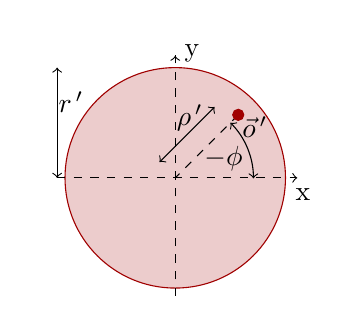
\begin{tikzpicture}[node distance=4em, auto]
    % Background size
    \node[background] at (0,0.15cm) {};

    % circle
    \draw[red1, fill=red1!20] (0,0) circle (1.4);

    % Draw axis
    \draw [->, dashed] (-1.5,0) |- (1.55,0) node [xshift=0.2em, yshift=-0.6em] {x};
    \draw [->, dashed] (0,-1.5) |- (0,1.55) node [xshift=0.6em, yshift=0.1em] {y};
    \draw [-, dashed] (0.8,0.8) -- (0,0);

    % point
    \draw[fill=red1, color=red1] (0.8,0.8) circle (2pt) node [below, color=black, xshift=0.6em, yshift=0.1cm] {$\vec o'$};

    % sizes
    \path[<->]
        (-1.5,0.0) edge node [xshift=0.5em, yshift=0.75em, anchor=center] {$r'$} (-1.5,1.4)
        (-0.2,0.2) edge node [xshift=0.1em, yshift=0.6em, anchor=center] {$\rho'$} (0.5,0.9);

    % angles
    \draw[black, fill=none, <->] (0.7,0.7) arc (45:0:1) node [xshift=-0.38cm, yshift=0.25cm] {$-\phi$};
\end{tikzpicture}

    \caption{Camera view of the mirror.}
    \label{fig:robot_method_algorithms_mirror_sphere_front}
  \end{subfigure}\hfill
  \begin{subfigure}[]{0.3\textwidth}
    \centering
    % Define block styles
\tikzstyle{block} = [draw, rectangle, text centered, text width=10em, minimum height=0.5em, rounded corners=true]
\tikzstyle{arrowtext} = [text width=4em, text centered]
\tikzstyle{background} = [draw, rectangle, text centered, text width=3.5cm, minimum height=3.5cm, color=white]
\tikzstyle{arrow} = [draw, -latex]

\definecolor{red1}{RGB}{160,0,0}
\definecolor{green1}{RGB}{0,160,0}
\definecolor{blue1}{RGB}{0,0,160}
\definecolor{black}{RGB}{0,0,0}
\definecolor{white}{RGB}{255,255,255}

\usetikzlibrary{shapes.geometric,arrows,positioning}

	      
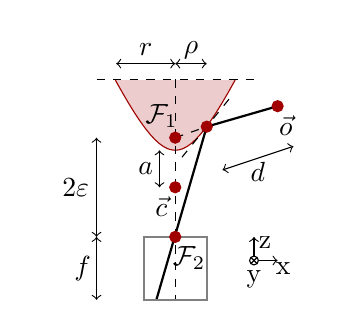
\begin{tikzpicture}[node distance=4em, auto]
    % Background size
    \node[background] at (0,-1.1cm) {};

    % hyperbola
    \pgfmathsetmacro{\e}{1.1};   % eccentricity
    \pgfmathsetmacro{\a}{1.1};
    \pgfmathsetmacro{\b}{(\a*sqrt((\e)^2-1)} 
    \draw[red1, fill=red1!20, yshift=-2.0cm] plot[domain=-1.2:1.2, rotate=90] ({\a*cosh(\x)},{\b*sinh(\x)});

	\coordinate (m) at (0.4,-0.6);
    \coordinate (o) at (1.3,-0.34);
    \coordinate (c) at (0,-1.37);
    \coordinate (v) at (0,-0.74);
    \coordinate (f) at (0,-2.00);
    \coordinate (cam) at (-0.24,-2.8);

    % Draw axis
    \draw [-, dashed] (0,0) |- (0,-2.8);
    \draw [-, dashed] (-1,0) |- (1,0);
	\draw [-, dashed] (v) -- (m);
	\begin{scope}[rotate around={51:(m)}]
			\draw[-, dashed] (0.4-0.5,-0.6) -- (0.4+0.5,-0.6);
	\end{scope}

    % Mini-Coordinate-System
    \draw [->] (1.0,-2.3) |- (1.3,-2.3) node [xshift=0.2em,yshift=-0.3em,anchor=center] {x};
    \draw [->] (1.0,-2.3) -- (1.0,-2.0) node [xshift=0.4em,yshift=-0.2em,anchor=center] {z};
    \draw [color=black, fill=white] (1.0,-2.3) circle(0.056) node [below] {y};
    \draw [-] (0.96,-2.34) -- (1.04,-2.26);
    \draw [-] (0.96,-2.26) -- (1.04,-2.34);

    % Light
    \draw[-, thick] (m) -- (cam);
    \draw[-, thick] (m) -- (o);

    % camera
    %\draw [-, thick, gray] (-0.5,-2.0)
    %    -- (0.5,-2.0)
    %    -- (0.3,-2.3)
    %    -- (-0.3,-2.3)
    %    -- (-0.5,-2.0);
    \draw [-, thick, gray] (0.4,-2.0) 
        -- (0.4,-2.8)
        -- (-0.4,-2.8)
        -- (-0.4,-2.0)
        -- cycle;

    % point
    \draw[fill=red1, color=red1] (m) circle (2pt) node [below, color=black, xshift=0.3em, yshift=0.1] {}; % was: $\hat{\vec o}$
    \draw[fill=red1, color=red1] (o) circle (2pt) node [below, color=black, xshift=0.3em, yshift=0.1] {$\vec{o}$};
    \draw[fill=red1, color=red1] (c) circle (2pt) node [below, color=black, xshift=-0.5em] {$\vec{c}$};
    \draw[fill=red1, color=red1] (v) circle (2pt) node [above, color=black, xshift=-0.5em] {$\mathcal{F}_1$};
    \draw[fill=red1, color=red1] (f) circle (2pt) node [below, color=black, xshift=0.5em] {$\mathcal{F}_2$};

    % sizes
    \path[<->]
        (-1.0,-0.74) edge node [xshift=-0.75em, anchor=center] {$2\varepsilon$} (-1.0,-2.0)
        (-1.0,-2.0) edge node [xshift=-0.5em, anchor=center] {$f$} (-1.0,-2.8)
        (-0.2,-0.9) edge node [xshift=-0.5em, anchor=center] {$a$} (-0.2,-1.37)
        (0.0,0.2) edge node [yshift=0.5em, anchor=center] {$\rho$} (0.4,0.2)
        (0.0,0.2) edge node [yshift=0.5em, anchor=center] {$r$} (-0.75,0.2)
        (0.6,-1.15) edge node [yshift=-0.5em, anchor=center] {$d$} (1.5,-0.85);
\end{tikzpicture}

    \caption{Side view of hyperbola mirror.}
    \label{fig:robot_method_algorithms_mirror_hyperbola_top}
  \end{subfigure}
  \caption{Sketch of a camera observing an object $\vec{o}$, which appears at position $\vec o'$ in the image plane (b). In Figure (c) the camera is pointed at a hyperbolic mirror.}
  \label{fig:robot_method_algorithms_mirror}
\end{figure}

\newcommand{\Fi}{\ensuremath{\mathcal{F}_1}}
\newcommand{\Fii}{\ensuremath{\mathcal{F}_2}}

The surface of a hyperbolic mirror is defined by
\begin{equation}
  \frac{y^2}{a^2} - \frac{x^2}{b^2} = 1 \quad,~a, b \R{1}
\end{equation}
with the semi-major axis $a$. 
The focal points $\mathcal{F}_{1,2}$ are set apart by \[{2\sqrt{a^2 + b^2} =: 2\epsilon}\] (\figref{fig:robot_method_algorithms_mirror_hyperbola_top}).
The robot's position is defined by the point in the middle of these two focal points.
The camera's focal point coincides with $\Fii$.
With ${\vec e}$ being the unit vector pointing from the reflection on the mirror towards the object's position $\vec o$:

\begin{equation}
  \nonumber
  \vec e_H(\vec o') =
    \frac{\left( s \, \vec o'_x, s \, \vec o'_y, \frac{a}{b} \sqrt{\rho^2 + b^2} - \varepsilon \right)^\intercal}
    {\left| \left( s \, \vec o'_x, s \, \vec o'_y, \frac{a}{b} \sqrt{\rho^2 + b^2} - \varepsilon \right)^\intercal \right|} \quad \text{,}
\end{equation}

the transformation $T_H$ is

\begin{equation}
  \nonumber
  \begin{aligned}
    T_H: & \vec o' \longmapsto \vec o : \\
    \vec o = & \vec c + R(\vec q)
    \left( \begin{array}{c}
             s o'_x\\
             s o'_y\\
             \frac{a}{b} \sqrt{\rho(\vec o')^2 + b^2}
           \end{array} + d \vec e_H(\vec o') \right) \quad \text{.}
    \end{aligned}
\end{equation}

and therefore the object position at a distance $d$ is defined as $\vec o = \vec r + R \left( \hat{\vec o} + \Di \vec e \right)$.
For the inverse transformation in polar coordinates, it can be shown that the radius $\rho'$ is given by

\begin{equation}
  \rho' = \frac{\left( \vec o - \vec c \right)_\rho}{\left( \vec o - \vec c \right)^2_\rho \cdot \varepsilon^2 / b^2 -1}
         \left( \left( \vec o - \vec c \right)_z \varepsilon + a \right) \quad \text{.}
\end{equation}

To simplify these expressions, the rotation matrix $R$ was left out.
Different camera orientations $\vec q$ are accounted for by rotating the vector $\left( \vec o - \vec c \right)$ before calculations.
The corresponding image position is now found as $\vec o' = \left( \rho \cos \phi, \rho \sin \phi \right)^\intercal$.





\subsubsection{Feature Set}

As already mentioned, features are first computed on the raw camera image.
Features are points in an image, which are easy to find, recognize, and track in consecutive frames --- usually areas rich in texture.
Afterwards, the optical flow is computed using these features.
There are numerous publications comparing different feature algorithms --- the most prominent algorithms include FAST~\cite{Rosten2006}, GFTT~\cite{shi1994}, ORB~\cite{rublee2011orb}, SIFT~\cite{lowe1999object}, and SURF~\cite{bay2006}.
Here, FAST is used as it offers a good trade-off between computational complexity and quality of found features~\cite{Elgayar2013175, Heinly2012}.
Then, the optical flow is estimated using a pyramidical implementation of the Lucas-Kanade method~\cite{bouguet2001pyramidal}.





\subsubsection{Motion and Depth Estimation}

Now, one can compute the robot's displacement (translation and rotation) between consecutive frames.
A list of all features for all frames is kept, which means the position of each feature relative to multiple robot positions is available.
This enables the robot to perform triangulation.
While in theory one would get a good estimate, real world experiments show that quite a lot of noise gets introduced.

Estimating the depth for $N$ features adds significant complexity to the problem.
Currently, \gls{ac:evo} tries to estimate the quadrocopter's 6d motion $M$ --- consisting of translation $\Delta \vec r$ and orientation $\Delta \vec q$.
Our problem has now increased to $N + 6$ dimensions.
Changes in the feature set from frame $\vec i_{i, t-1}$ to frame $\vec i_{i, t}$ provide $N$ equations, meaning features need to be tracked for at least $3$ consecutive frames.

\newcommand{\pr}{\ensuremath{{\,p}}}
\paragraph{Computing the feature correspondence}
\begin{enumerate}
  \item Depth $d_{i,t-1}$ and motion $M_{t}$ are initialized using previous data $d_{i,t-2}$ and motion $M_{t-1}$. The camera pose $P_{t-1}$, consisting of position $\vec c_{t-1}$ and rotation $\vec q_{t-1}$, is known.
  \item For every feature $i$, calculate the global position $\vec o_{i,t - 1}$ using the depth $d_{i,t-1}$, the image coordinates $\vec o'_{i,t - 1}$ and the camera pose $P_{t-1}$ using the transformation $T_H$.
  \item Apply the inverse motion to all global positions $\vec o_{i, t-1}$. This results in the predicted global positions $\vec o^\pr_{i, t}$.
  \item Use the inverse transformation $T^{-1}_H$, to compute the predicted image position $\vec{o}'^{p}_{i, t} = T^{-1}_H \left( \vec{o}^\pr_{i, t} \right)$.
  \item Lastly, the environment as well as all global features is considered to be static. Therefore, one may minimize the sum of the squared distances for the last $L$ time steps:
  \[\textrm{SD} \left( d_{i, t}, M \right) = \sum_{i=0}^{N} \sum_{t=-L}^{0} \left\lVert \vec o'_{i,t} - \vec o^{\prime p}_{i,t} \right\rVert^2 .\]
\end{enumerate}

\paragraph{Estimating the depth with the forward estimation}
\begin{enumerate}
  \item Perform step 1. and 2. from the inverse estimation.
  \item The goal is to find the new depth $d_{i, t}$ based on the previous estimate $d_{i, t-1}$.
    %In the pinhole model, the depth is defined as the $y$-component of the difference between the object position $\vec o_i$ and the camera position $\vec c$:
    %${d_{t} = \left( R \left( \Delta \vec{q}_{t} \right) \left( \vec o - \vec c_{t-1} - \Delta \vec c_t \right) \right)_y \, \text{.}}$
    In omnidirectional mirror models, the depth is
    \[{d_{t} = \left\lVert R \left( \Delta \vec{q}_{t} \right) \left( \vec o - \vec c - \Delta \vec c_t \right) - \hat{\vec o}^{\,p} \, \right\rVert \, \text{.}}\]
    The new reflection point $\hat{\vec o}^p$ is calculated with the inverse transformation $T^{-1}_H$.
  \item Compute the new predicted pose $P_{t} = P_{t-1} + M_{t}$.
  \item Compute predicted global positions $\vec o^\pr_{i, t=0}$ for every feature $i$ based on the camera model.
  \item The positions $\vec o_{i, t}$ and $\vec o^\pr_{i, t}$ should be equal for corresponding features $i$. We use this to minimize the sum of the squared distances
\begin{equation}
  \nonumber
  \textrm{SD} \left( d_{i, t}, M \right) = \sum_{i=0}^{N} \sum_{\tau=-L}^{0} \left\lVert \frac{ \vec o_{i,t-\tau} - \vec{o}^\pr_{i, t-\tau}}{d_{i,t-\tau}} \right\rVert^2.
\end{equation}
Now, $d_{i,t}^{-1}$ weights all summands consistently as the position-error scales linearly with $d$.
\end{enumerate}





\subsubsection{Maximum angular resolution}

Given a fixed camera resolution of $\unit[480 \times 480]{px}$ one can now compute the projection of the hyperbola mirror onto the camera. 
It is assumed that the object is at a distance of $\unit[2]{m}$ and five pixels width to separate it from adjacent objects are required. 
After straightforward application of the above formulas, the limit is derived as approximately $1.3\degree$.
